%%%%%%%%%%%%%%%%%%%%%%%%%%%%%
% Courtesy of Charlotte Olsen, '23 and past graduates for this updated version of the Rutgers template!
%%%%%%%%%%%%%%%%%%%%%%%%%%%%%


\documentclass[11pt]{ruthesis}
\special{papersize=8.5in,11in}

\usepackage[numbers,sort&compress]{natbib}
\usepackage{notoccite} % citations in the LoF/LoT do not set the bibliography order
\usepackage{url}

\usepackage{comment}

\usepackage{aastex_hack}
%\usepackage{deluxetable} 
\usepackage{graphicx}
\usepackage{tabularx}
\usepackage{rotating}
\usepackage{lscape,longtable}
\usepackage[T1]{fontenc}
\usepackage{makecell}
\usepackage[T1]{fontenc}
%\usepackage{tgbonum}
%\usepackage{ulem}

\setlength{\unitlength}{1.0cm}

% Load packages; ambssymb is for extra fonts, such as blackboard
\usepackage{latexsym}
\usepackage{amsmath}
\usepackage{amssymb}
\usepackage{amsbsy}
\usepackage{xcolor}
\usepackage{setspace}
\usepackage{xspace}
\usepackage{soul}
\usepackage{multirow}
\usepackage{booktabs}
\usepackage{bigdelim}
\usepackage{tikz}
\usepackage{tikz-3dplot}
\usepackage{physics}
\usepackage[compat=1.1.0]{tikz-feynman}
\usepackage[compat=1.1.0]{tikz-feynhand}
\usepackage{xcolor}
\usepackage[outline]{contour} % glow around text
\contourlength{0.9pt}
\usepackage{cancel}
\usepackage{slashed} % Feynman slash notation, \slashed{p}
\usepackage{listofitems} % to create arrays with \readlist
\usepackage{ifthen} % for \whiledo
\usepackage{siunitx} % for \SI
\usetikzlibrary{decorations.pathmorphing} % for snake, coil, zigzag
\usetikzlibrary{fpu} % for higher floating-point precision
\usetikzlibrary{angles,quotes} % for pic (angle labels)
\usetikzlibrary{arrows.meta} % for arrow head size
\usetikzlibrary{bending} % for bending arrow head
\usetikzlibrary{3d} % for canvas is
\usetikzlibrary{patterns,decorations.pathreplacing} % hatching and braces (App. torchstrap)

\pgfkeys{
  /pgf/fpu/output format=fixed, % fpu floating-point format
  /pgf/number format/precision=2 % two decimals
}

% Run-in \paragraph headings: same style as ruthesis' subsubsection, preceded by a bullet
\makeatletter
\renewcommand{\paragraph}{\@startsection{paragraph}{4}{\z@}{-3.25ex plus -1ex minus -.2ex}{1.5ex plus .2ex}{\normalsize\bfseries\textbullet\enspace}}
\makeatother

% Allow slightly looser lines instead of overfull boxes (long unbreakable math, PYTHIA\mbox{-}6)
\setlength{\emergencystretch}{2em}

% Define Italic Sans Serif font (for tensors)
\DeclareMathAlphabet{\mathsfsl}{OT1}{cmss}{m}{sl}


%sectionbib option ensures that the bibliography is treated as a 
% section in your chapter, and not a new chapter.
% \usepackage[sectionbib,authoryear]{natbib} 
% \bibliographystyle{apj}

% Normal astronomical referencing is usually in the form (Smith
% 1999), this is to remove the extra comma in  (Smith, 1999).
%\bibstyle{aa}
%\citestyle{aa}   % author-year; disabled in favour of numeric citations

% to compile only the sections we are currently working on.
%\includeonly{warp1,summary,appendix_warpA,appendix_warpB}
%\includeonly{intro}

%to show notes on the margin, {\baselinestretch}{1} is because in 
% case double-space is used in the main text.
%\long\def\Notes#1{\marginpar{\renewcommand{\baselinestretch}{1} \tiny #1}}
%\long\def\Notes#1{\relax}
%\long\def\Ignore#1{\relax}
%\long\def\Comment#1{{\it\footnotesize #1}}

% The page number in Rutgers thesis format is so high up in the
% page that normal printers can not print it out! The following is to
% lower page numbers down a bit, so we can see them in a draft
% version to the committee members. Do NOT use this change in the
% FINAL version to be submitted to the Graduate School.
%\addtolength{\topmargin}{0.3cm}


% Editing color by co-authors
\definecolor{myred}{rgb}{0.7,0.1,0.1}
\def\eg#1{\textcolor{myred}{Advisor: #1}}
\definecolor{myblue}{rgb}{0.,0.4,0.7}
\def\cao#1{\textcolor{myblue}{Student: #1}}

%\draft
\setcounter{tocdepth}{1}

%commands
\newcommand{\addTwoPanelFig}[3]{
	\begin{figure}[H]
		\centering
		\includegraphics[width = 0.7\linewidth]{#1}
		\caption{#2}
		\label{#3}
	\end{figure}
}
\newcommand{\addTwoPanelInFig}[1]{\includegraphics[width = 0.68\linewidth]{#1}}
\newcommand{\addOnePanelInFig}[2]{\includegraphics[width = #2\linewidth]{#1}}


% energy units, collision systems
\newcommand{\GeVc}{GeV/\(c\)\xspace}
\newcommand{\MeVc}{MeV/\(c\)\xspace}
\newcommand{\Gevcsq}{\ensuremath{\mathrm{GeV}/c^{2}}}
\newcommand{\etaphi}{\ensuremath{(\eta,\phi)}~}
\newcommand{\Pt}[1]{\ensuremath{p_{\mathrm{T, #1}}}}
\newcommand{\ptRange}[3]{\ensuremath{#2 \leq p_{\mathrm{T, #1}} < #3~\mathrm{GeV}/c}}
\newcommand{\ptGeq}[2]{\ensuremath{p_{\mathrm{T, #1}} \geq #2~\mathrm{GeV}/c}}
\newcommand{\EtTower}{\ensuremath{E_{\mathrm{T, tower}}}}
\newcommand{\pp}{\ensuremath{p + p}~}
\newcommand{\PbPb}{Pb+Pb\xspace}
\newcommand{\AuAu}{Au+Au\xspace}
\newcommand{\qqToqq}{\ensuremath{qq\rightarrow qq}~}
\newcommand{\ggTogg}{\ensuremath{gg\rightarrow gg}~}
\newcommand{\sPP}[2]{\ensuremath{\sqrt{s} = #1\ \mathrm{#2}}}
\newcommand{\sNN}[2]{\ensuremath{\sqrt{s_{\mathrm{NN}}} = #1\ \mathrm{#2}}}

\newcommand{\rhoR}{\ensuremath{\rho({\mathbf{r}})}}
\newcommand{\RAA}{\ensuremath{R_{\rm AA}}}
\newcommand{\Et}{\ensuremath{E_{\rm T}}\xspace}
\newcommand{\kt}{\ensuremath{k_{\rm T}}\xspace}
\newcommand{\ptRecoJet}{\ensuremath{p_{\mathrm{T, jet}}^{\rm RECO}}\xspace}
\newcommand{\ptGenJet}{\ensuremath{p_{\mathrm{T, jet}}^{\rm GEN}}\xspace}
\newcommand{\dphi}{\ensuremath{\Delta\phi}\xspace}
\newcommand{\deta}{\ensuremath{\Delta\eta}\xspace}
\newcommand{\dvphi}{\ensuremath{\Delta\varphi}\xspace}
\newcommand{\zvtx}{$z_{\mathrm{vtx}}$\xspace}

% labels for LaTeX
\newcommand{\sref}[1]{section~\ref{#1}}
\newcommand{\fref}[1]{figure~\ref{#1}}
\newcommand{\tref}[1]{table~\ref{#1}}
\newcommand{\eref}[1]{equation~\ref{#1}}
\newcommand{\Sref}[1]{Section~\ref{#1}}
\newcommand{\Fref}[1]{Figure~\ref{#1}}
\newcommand{\Tref}[1]{Table~\ref{#1}}
\newcommand{\Eref}[1]{Equation~\ref{#1}}

\newcommand{\dndydpt}{${\rm d}^2N/({\rm d}y {\rm d}p_{\rm t})$}
\newcommand{\dNtrigdphideta}{$\frac{1}{N_{\mathrm{t}}} \frac{d^2N}{d\Delta\phi d\Delta\eta}$\xspace}
\newcommand{\dNeventdphideta}{$\frac{1}{N_{\mathrm{e}}} \frac{d^2N}{d\Delta\phi d\Delta\eta}$\xspace}
\newcommand{\dNdphi}{$\frac{dN}{d\phi}$}
\newcommand{\ns}{near-side\xspace}
\newcommand{\as}{away-side\xspace}
\newcommand{\Rn}{$r_n$\xspace}
\newcommand{\midplane}{mid-plane\xspace}
\newcommand{\inplane}{in-plane\xspace}
\newcommand{\outplane}{out-of-plane\xspace}
\newcommand{\Midplane}{Mid-plane\xspace}
\newcommand{\Inplane}{In-plane\xspace}
\newcommand{\Outplane}{Out-of-plane\xspace}

% commands from background papers
\newcommand{\Beff}{$\tilde{\beta^{R}}$\xspace}
\newcommand{\vn}{$v_{n}$\xspace}
\newcommand{\vnt}{$v_{n}^{t}$\xspace}
\newcommand{\vneff}{$\tilde{v}_{n}^{t}$\xspace}
\newcommand{\vneffnot}{$\tilde{v}_{n}$\xspace}
\newcommand{\vnaeff}{$\tilde{v}_{n}^{a}$\xspace}
\newcommand{\vnteff}{$\tilde{v}_{n}^{t}$\xspace}
\newcommand{\vnum}[1]{$v_{#1}$\xspace}
\newcommand{\vnumtrigger}[1]{$v_{#1}^{t}$\xspace}
\newcommand{\vnumeff}[1]{$\tilde{v}_{#1}$\xspace}
\newcommand{\vnumeffsq}[1]{$\tilde{v}_{#1}^{2}$\xspace}
\newcommand{\vnumeffR}[1]{$\tilde{v}_{#1}^{R,t}$\xspace}
\newcommand{\vnumeffassoc}[1]{$\tilde{v}_{#1}^{a}$\xspace}
\newcommand{\vnumefftrigger}[1]{$\tilde{v}_{#1}^{t}$\xspace}
\newcommand{\vneffR}{$\tilde{v}_{n}^{R,t}$\xspace}
\newcommand{\vnsq}{$\tilde{v}_{n}^{\mathrm{a}}\tilde{v}_{n}^{\mathrm{t}}$\xspace}
\newcommand{\vntrigger}{$v_{n}^{\mathrm{t}}$\xspace}
\newcommand{\vnassoc}{$v_{n}^{\mathrm{a}}$\xspace}
\newcommand{\vnefftrigger}{$\tilde{v}_{n}^{\mathrm{t}}$\xspace}
\newcommand{\vneffassoc}{$\tilde{v}_{n}^{\mathrm{a}}$\xspace}

\newcommand{\pttrigrange}[2]{$#1 < p_{\mathrm{T, jet}} < $ #2 GeV/$c$\xspace}
\newcommand{\ptassocrange}[2]{$#1 < p_{\mathrm{T, assoc}} <$ #2 GeV/$c$\xspace}

\renewcommand{\thepart}{\Alph{part}}

% from thesis commands
\newcommand{\commented}[1]{\textcolor{red}{\textbf{\hl{#1}}}}  % add sent, paragraph, section on #topic
\newcommand{\CITETHIS}{\textcolor{red}{\textbf{\hl{CITE!}}}} % cite this!

% add struts used for tables
\newcommand\Tstrut{\rule{0pt}{2.6ex}}         % = `top' strut
\newcommand\Bstrut{\rule[-0.9ex]{0pt}{0pt}}   % = `bottom' strut

% for asymmetric errors in table
%\newcommand{\tol}[3]{\ensuremath{\si{#1}^{\thinspace+\num{#2}}_{-\num{#3}}}} %Formula for tolerancing
\def\tol#1#2#3{\hbox{\rule[-1.5mm]{0pt}{15pt}${#1}^{+{#2}}_{-{#3}}$}}

% ---------------- CUSTOM MACROS ----------------
% Macro for Section Headers
% COLORS
\colorlet{protoncol}{red!68!black!80}
\colorlet{neutroncol}{green!68!black!80}
\colorlet{participantcol}{red!75!black!85}
\colorlet{spectatorcol}{blue!65!black!85}
\colorlet{photoncol}{yellow!85!orange!95!black}
\colorlet{veccol}{green!50!black}
\colorlet{myred}{red!70!black}
\colorlet{mycontourred}{red!55!black!3} % for contour
\colorlet{mycontourred2}{red!55!black!6} % for contour
\colorlet{myblue}{blue!70!black}
\colorlet{mydarkred}{red!40!black}
\colorlet{mydarkblue}{blue!30!black}
\colorlet{CMScol}{red!80!black}
\colorlet{ATLAScol}{blue!80!black}

\tikzstyle{axis}=[->,thick,line cap=round]
\tikzstyle{detector}=[thick,draw=mydarkred,rotate around z=\ang]
\tikzstyle{beam pipe}=[draw=blue!20!black!50,fill=blue!20!black!10,rotate around z=\ang]
\tikzstyle{detector surface}=[red!60!black!10,opacity=0.5,rotate around z=\ang]

\tikzstyle{cone}=[thin,blue!50!black,fill opacity=0.8]
\tikzstyle{calo}=[draw=blue!60!green!50!black,fill=blue!60!green!90!black!70,
line width=0.6,rounded corners=0.2]
\tikzstyle{calobg}=[draw=none, fill=black, fill opacity=0.35,line width=0.6,rounded corners=0.2]
\tikzstyle{ecal}=[calo,draw=red!90!green!60!black,fill=red!85!green!90!black!80]

\newif\ifnucpart % nucleus pic: colour nucleons as participants/spectators
% STYLES
\tikzset{
	>=latex, % for LaTeX arrow head
	eta line/.style={->,black!60!red,thick,line cap=round},
	theta node/.style={black,pos=0.7,fill=white,scale=0.8,
		inner sep=1.5pt,rounded corners=3pt},
	mysmallarrow/.style={-{Latex[length=3,width=2.5]},draw=black,line width=0.6,
		angle radius=45,angle eccentricity=1.1},
	vector/.style={->,thick,green!60!black},
	photon/.style={->,line width=0.7,line cap=round,photoncol,decorate,decoration={
			snake,amplitude=.4mm,segment length=2.2mm,post length=1.5mm}
	},
	ball/.style={
		circle,draw=none,ball color=#1,postaction={
			fill=#1,fill opacity=0.8,draw=#1!40!black,line width=0.04}
	},
	ball/.default=protroncol,
	% participant/spectator colouring: nucleons with local y in [ymin,ymax] are participants
	nucleus participants/.is if=nucpart,
	nucleus ymin/.store in=\nucymin, nucleus ymin=0,
	nucleus ymax/.store in=\nucymax, nucleus ymax=0,
	pics/nucleus/.style={%
		code={%
			\ifnucpart
				\fill[spectatorcol] (0,0) circle(0.86*\R); % background to fill any holes
				\begin{scope}
					\clip (0,0) circle(0.86*\R);
					\fill[participantcol] (-\R,\nucymin) rectangle (\R,\nucymax);
				\end{scope}
			\else
				\fill[protoncol] (0,0) circle(0.86*\R); % background to fill any holes
			\fi
			\pgfmathsetmacro\Rball{0.18*\R} % ball radius
			\pgfmathsetmacro\Rcorr{\R-\Rball} % subtract ball radius
			\pgfmathsetmacro\C{min(1/(4*\Rcorr),0.24)} % put balls at edges closer in to create 3D ball effect
			\pgfmathsetmacro\D{1-4*\C*\Rcorr} % discriminant
			\pgfmathsetmacro\Rs{2*(\Rcorr)/(1+sqrt(\D)} % scaled total radius
			\message{^^J R=\R, R=\Rcorr, Rs=\Rs, C=\C, D=1-4cR=\D (must be >0)}
			\foreach \lay [evaluate={
				\r=\Rs*(\lay-0.05)/\Nlay; % ring radius
				\rC=\r-\C*\r*\r; % reduce outer radii to create 3D effect
				\aR=3*rand; % random angular offset
				\Nring=int(round(2*\rC*\N/(\Rs*(\Nlay+1)*(1-\C*\Rs*(2*\Nlay+1)/(3*\Nlay))))) % number of balls on this ring
			}] in {\Nlay,...,1}{
				\message{^^J N=\N, Nlay=\Nlay, Nring=\Nring, r=\r}
				\shufflelist{\Nring} % get shuffled list of sequence 1,...,\Nring
				\foreach \i [evaluate={
					\p=(rand+1)/2<0.39?1:0; % 0: neutron, 1: proton
					\is=int(\shuffledlist[\i]); % shuffled index
					\aB=\aR+360*(\is/\Nring)+2*rand/\Nring; % ball angle plus random offset
					\rB=\rC+0.04*rand; % ball radius plus random radial offset
					\yB=\rB*sin(\aB); % local vertical position
					\q=(\yB>=\nucymin && \yB<=\nucymax)?1:0 % 0: spectator, 1: participant
				}] in {1,...,\Nring}{
					%\message{^^J is=\is, i=\i, a=\aB, p=\p}
					\ifnucpart
						\fill[ball=\ifodd\q participantcol\else spectatorcol\fi]
						(\aB:\rB) circle(\Rball);
					\else
						\fill[ball=\ifodd\p protoncol\else neutroncol\fi]
						(\aB:\rB) circle(\Rball);
					\fi
				}
			}
			\ifnucpart
				\pgfmathsetmacro\q{(0>=\nucymin && 0<=\nucymax)?1:0}
				\fill[ball=\ifodd\q participantcol\else spectatorcol\fi] (0,0) circle(\Rball);
			\else
				\fill[ball=protoncol] (0,0) circle(\Rball);
			\fi
			\foreach \ang in {0,60,90,120,180,-60,-90,-120}{
				\coordinate (-\ang) at (\ang:\R+1.3*\Rball);
			}
		}
	}
}
\def\shufflelist#1{ % get shuffled list of sequence 1,...,#1
	%\message{^^JShuffle list}
	\pgfmathsetmacro\tmplist{random(1,#1)} % first random item
	\readlist*\shuffledlist\tmplist % convert to array
	\newboolean{unique}
	\whiledo{\shuffledlistlen<#1}{ % try until list is of length = #1
		\pgfmathsetmacro\rx{random(1,#1)} % generate new random item
		\setboolean{unique}{true}
		\foreachitem \x \in \shuffledlist{ % loop over previous elements
			\ifnum \x=\rx % look if new number in list
			\setboolean{unique}{false} % already in list
			\breakforeach % stop looking and try again in next iteration
			\fi
		}
		\ifthenelse{\boolean{unique}}{ % found unique item !
			\xdef\tmplist{\tmplist,\rx} % add new unique item
			\readlist*\shuffledlist\tmplist % convert to array
		}{}
	}
}

\newcommand*{\vv}[1]{\vec{\mkern0mu#1}} % aligned vector arrow
\newcommand{\vhead}[1]{\textcolor[HTML]{B32222}{\sffamily\small\uppercase{#1}}}

% Macro for 3-point vertices 
% Args: #1=bottom-left style, #2=bottom-left label, #3=top-left style, #4=top-left label, #5=right style, #6=right label
\newcommand{\threevertex}[6]{%
	\begin{tikzpicture}[baseline=0, thick]
		\begin{feynman}
			\vertex [circle, fill=black, minimum size=3.5pt, inner sep=0pt] (v) at (0,0) {};
			\vertex (i1) at (240:1.5) {\(#2\)};
			\vertex (i2) at (120:1.5) {\(#4\)};
			\vertex [circle, fill=black, minimum size=2.5pt, inner sep=0pt] (o) at (1.5,0) {};
			\diagram* {
				(i1) -- [#1] (v) -- [#3] (i2),
				(v) -- [#5, edge label'=\(#6\)] (o)
			};
		\end{feynman}
	\end{tikzpicture}%
}

\newcommand\jetcone[4]{
	\pgfmathanglebetweenpoints{\pgfpointanchor{#1}{center}}{\pgfpointanchor{#2}{center}}
	\edef\tmpang{\pgfmathresult}
	\coordinate (tmpO) at ($(#1)+(\tmpang:0.02)$); % center
	\coordinate (tmpC) at ($(#2)+(\tmpang-180:{abs(#4)+0.4})$); % center
	\coordinate (tmpL) at ($(tmpC)+(\tmpang+90:#3)$); % left corner
	\coordinate (tmpR) at ($(tmpC)+(\tmpang-90:#3)$); % right corner
	\draw[thin,blue!50!black,fill opacity=0.8, %,fill=blue!50!black!30
	top color=blue!50!black!50,bottom color=blue!50!black!60,shading angle=\tmpang,rotate=\tmpang]
	%(tmpR) arc(90:-90:{#4} and {#3});
	(tmpC) ellipse({#4} and {#3});
	\begin{scope}
		\clip[rotate=\tmpang] (tmpR) -- (tmpO) -- (tmpL) arc(90:-90:{#4+0.6} and {#3});
		\draw[vector] (tmpO) -- (#2);
	\end{scope}
	\draw[thin,blue!50!black,fill opacity=0.8, %,fill=blue!50!black!30
	top color=blue!50!black!30,bottom color=blue!40!black!50,shading angle=\tmpang,rotate=\tmpang]
	(tmpL) arc(90:270:{#4} and {#3}) -- (tmpO) -- cycle;
}

% Collider detector coordinate system
\newcommand{\detectorCoordinateSystem}{
\tdplotsetmaincoords{122.61461}{113.95680}
\begin{tikzpicture}[scale=2.8,tdplot_main_coords,rotate=76.53217]
	% VARIABLES
	\def\thetavec{60}
	\def\phivec{60}
	\def\L{3.1}     % detector length
	\def\R{0.75}    % detector cylinder radius
	\def\l{4.1}     % beam pipe length
	\def\r{0.04}    % beam pipe radius
	\def\rt{0.042}  % beam pipe radius + line thickness
	\def\xmax{1}    % maximum x axis
	\def\ymax{1.05} % maximum y axis
	\def\zmin{-\l/2-0.2} % minimum z axis
	\def\zmax{\l/2+0.3}  % maximum z axis
	\coordinate (O) at (0,0,0);
	\coordinate (Z) at (0,0,\L/2);
	\tdplotsetcoord{O''}{0.018}{90}{\phivec} % shifted origin for the pT arrow
	% |p| is chosen so the vector lands on the barrel surface: its transverse
	% projection (Pxy) then has radius exactly \R, so the beam-parallel line
	% through (Pxy) and (P) meets the +z endcap on its rim, at (Prim).
	\pgfmathsetmacro{\Rvec}{\R/sin(\thetavec)}
	\tdplotsetcoord{P}{\Rvec}{\thetavec}{\phivec}
	\coordinate (Prim) at ({\R*cos(\phivec)},{\R*sin(\phivec)},\L/2);
	
	% CYLINDER behind
	\def\ang{24} % rotate lines to simulate cylinder
	\fill[top color=red!50!black!4,bottom color=red!60!black!2,rotate around z=\ang]
	(0,\R,\L/2) --++ (0,0,-\L) arc(90:270:\R) --++ (0,0,\L) arc(270:90:\R) -- cycle;
	\fill[detector surface] % transverse plane at z=L/2
	(0,0,\L/2) --++ (0,\R,0) arc(90:270:\R) -- cycle;
	\fill[detector surface] % transverse plane at z=-L/2
	(0,0,-\L/2) --++ (0,\R,0) arc(90:270:\R) -- cycle;
	\tdplotdrawarc[detector,thin]{(0,0,\L/2)}{\R}{0}{360}{}{} % transverse plane at z=L/2
	\tdplotdrawarc[detector]{(0,0,-\L/2)}{\R}{0}{360}{}{} % transverse plane at z=-L/2
	\draw[detector,thin] % transverse plane at z=0
	(90:\R) arc (90:270:\R);
	\draw[detector,very thin] % transverse plane at z=0, top piece
	(90:\R) arc (90:90-\ang:\R);
	\draw[detector] (0,0,-\L/2)++(90:\R) --++ (0,0,\L); % top horizontal along z
	\draw[detector] (0,0,-\L/2)++(-90:\R) --++ (0,0,\L); % bottom horizontal along z
	
	% BEAM PIPE
	\tdplotdrawarc[beam pipe]{(0,0,-\l/2)}{\r}{0}{360}{}{}
	\draw[beam pipe] % beam pipe, thinner in middle
	(0,\r,-\l/2) -- (0,\r,-0.2*\l) -- (90:0.5*\r)
	-- (0,\r,0.2*\l) -- (0,\r,0.5*\l) arc(90:-90:\r)
	-- (0,-\r,0.2*\l) -- (-90:0.5*\r) --
	(0,-\r,-0.2*\l) -- (0,-\r,-\l/2) arc(-90:90:\r);
	\draw[beam pipe] (0,0,\l/2) circle(\r);
	
	% AXES
	\draw[axis] (0,0,0) -- (0,0,\zmax) node[above=2pt,right=1pt]{$z$}; % long
	\fill[CMScol] (O) circle(0.5pt) node[below=5pt] {IP};
	\draw[axis,-] (0,0,\zmin) -- (0,0,-0.020); % long
	\draw[axis] (0,0.019,0) -- (0,\ymax,0) node[above=1pt,right=1pt]{$y$};
	\draw[axis] (0.022,0,0) -- (\xmax,0,0) node[below=2pt,right=1pt]{$x$};
	
	% LABELS
	\node[mydarkred,above=1pt] at (0,\ymax,0) {$\eta=0$};
	\node[mydarkred,above=4pt,rotate around z=\ang] at (0,\R,0.30*\L) {$\eta>0$};
	\node[mydarkred,above=4pt,rotate around z=\ang] at (0,\R,-0.30*\L) {$\eta<0$};
	\node[mydarkred,left=1pt] at (0,0,\zmax) {$\eta=+\infty$};
	\node[mydarkred,right=1pt] at (0,0,\zmin) {$\eta=-\infty$};
	
	% CYLINDER front
	\draw[beam pipe,fill=none] (0,\r,-\l/2) arc(90:-90:\r);
	\fill[detector surface] % transverse plane at z=L/2
	(0,\rt,\L/2) --++ (0,\R-\rt,0) arc(90:-90:\R) --++ (0,\R-\rt,0) arc(-90:90:\rt);
	\fill[detector surface] % transverse plane at z=-L/2
	(0,\rt,-\L/2) --++ (0,\R-\rt,0) arc(90:-90:\R) --++ (0,\R-\rt,0) arc(-90:90:\rt);
	\tdplotdrawarc[detector]{(0,0,\L/2)}{\R}{-90}{90}{}{}
	\tdplotdrawarc[detector]{(0,0,-\L/2)}{\R}{-90}{90}{}{}
	\draw[beam pipe,fill=none] (0,\r,\l/2) arc(90:-90:\r);
	\draw[detector,very thin] % transverse plane at z=0, front piece
	(90-\ang:\R) arc (90-\ang:-90:\R);
	
	% VECTORS
	\draw[dashed,myred] (Pz) -- (P);
	\draw[dashed,myred,line join=round] (Py) -- (Pxy) -- (P) -- (Prim);
	\draw[dashed,myred] (Z) -- (Prim); % endcap radius at azimuth \phivec
	\draw[->,red,line cap=round] (O'') -- (Pxy) node[below=1pt,right=1pt] {$\vv{p}_\mathrm{T}$};
	\draw[->,red] (O) -- (P) node[above=1pt,left=1pt] {$\vv{p}$};
	
	% ANGLES
	% Each angle is drawn twice: once as the arc itself (no label), then as a
	% label-only pass with "draw=none" at a larger radius, so the label sits
	% radially outside the arc -- on the far side from the arc's centre.
	\def\labelgap{0.16} % radial offset of an angle label beyond its arc
	\tdplotdrawarc[thick,mycontourred]{(O)}{0.22}{4}{0.7*\phivec}{}{} % contour
	\tdplotdrawarc[->]{(O)}{0.22}{0}{\phivec}{}{}
	\tdplotdrawarc[draw=none]{(O)}{0.22+\labelgap}{0}{\phivec}
	{}{\contour{mycontourred}{$\phi$}}
	\tdplotdrawarc[->,rotate around z=\phivec-90,rotate around y=-90]
	{(O)}{0.42}{0}{\thetavec}{}{}
	\tdplotdrawarc[draw=none,rotate around z=\phivec-90,rotate around y=-90]
	{(O)}{0.42+\labelgap}{0}{\thetavec}{}{$\theta$}
	\tdplotdrawarc[-{>[bend=1]},rotate around z=\phivec-90,rotate around y=-90,line cap=round]
	{(O)}{0.34}{90}{\thetavec}{}{}
	\tdplotdrawarc[draw=none,rotate around z=\phivec-90,rotate around y=-90]
	{(O)}{0.34+\labelgap}{90}{\thetavec}{}{$\eta$}
	\draw[mydarkred,line cap=round] (0.004,0,\L/2) --++ (\R,0,0); % phi reference at z=L/2
	\tdplotdrawarc[thick,mycontourred2]{(Z)}{0.22}{4}{0.7*\phivec}{}{} % contour
	\tdplotdrawarc[->]{(Z)}{0.22}{0}{\phivec}{}{}
	\tdplotdrawarc[draw=none]{(Z)}{0.22+\labelgap}{0}{\phivec}
	{}{\contour{mycontourred2}{$\phi$}}
	
\end{tikzpicture}
}

% Macro for a propagator (2-point function)
% Args: #1=edge style, #2=left label, #3=right label, #4=momentum label
\newcommand{\propagator}[4]{%
	\begin{tikzpicture}[baseline=0, thick]
		\begin{feynman}
			\vertex (l) at (-1.1,0) {\(#2\)};
			\vertex (r) at ( 1.1,0) {\(#3\)};
			\diagram* { (l) -- [#1, edge label=\(#4\)] (r) };
		\end{feynman}
	\end{tikzpicture}%
}

% Macro for a Y-shaped 3-point vertex: one leg up, two legs down.
% The two lower legs are drawn as a single line THROUGH the vertex, so that
% fermion/ghost arrows follow the flow (down-left in, down-right out).
% Args, per leg: style / end label / momentum label (empty momentum = no label)
%   #1 #2 #3 = up leg,  #4 #5 #6 = lower-left leg,  #7 #8 #9 = lower-right leg
\newcommand{\yvertex}[9]{%
	\begin{tikzpicture}[baseline=0, thick]
		\begin{feynman}
			\vertex [circle, fill=black, minimum size=3.5pt, inner sep=0pt] (v) at (0,0) {};
			\vertex (u) at (90:1.5) {\(#2\)};
			\vertex (dl) at (215:1.5) {\(#5\)};
			\vertex (dr) at (325:1.5) {\(#8\)};
			\diagram* {
				(dl) -- [#4] (v) -- [#7] (dr),
				(v) -- [#1] (u),
			};
		\end{feynman}
		% momentum labels, placed by hand so the two lower ones stay apart
		\node[anchor=east] at ([xshift=-2pt]90:0.85) {\(#3\)};
		\node[anchor=south] at ([yshift=3pt]215:0.80) {\(#6\)};
		\node[anchor=south] at ([yshift=3pt]325:0.80) {\(#9\)};
	\end{tikzpicture}%
}

% Collinear factorization of a hadron-hadron hard scattering:
% the two incoming hadrons (double lines) each supply a parton carrying a
% fraction x of the hadron momentum, drawn from the parton distributions
% f_i(x_1), f_j(x_2); the partons enter the hard cross section
% sigma-hat_ij(alpha_s), and the beam remnants / outgoing partons leave as
% three-line legs.  Takes no arguments; use inside a figure.
\newcommand{\factorizationdiagram}{%
	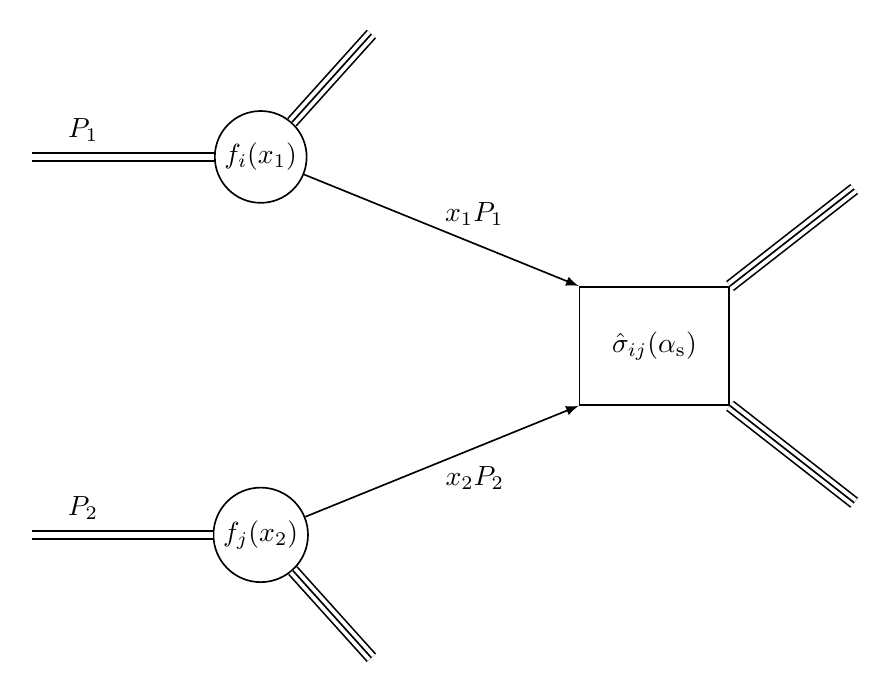
\begin{tikzpicture}[
			>=latex, line width=0.6pt,
			hadron/.style={double,double distance=2.2pt}, % incoming hadron: two lines
			triple/.style={double,double distance=3.4pt}, % outer pair of a three-line leg
		]
		% --- parton distributions and the hard-scattering blob
		\node[draw,circle,inner sep=2pt] (p1) at (0, 2.4) {$f_i(x_1)$};
		\node[draw,circle,inner sep=2pt] (p2) at (0,-2.4) {$f_j(x_2)$};
		\node[draw,minimum width=1.9cm,minimum height=1.5cm,inner sep=2pt]
		(sig) at (5.0,0) {$\hat{\sigma}_{ij}(\alpha_{\rm s})$};

		% --- endpoints of the beam remnants and the outgoing partons
		\path (p1) ++(48:2.1) coordinate (rem1);
		\path (p2) ++(-48:2.1) coordinate (rem2);
		\path (sig.north east) ++(38:2.0) coordinate (out1);
		\path (sig.south east) ++(-38:2.0) coordinate (out2);

		% --- incoming hadrons
		\draw[hadron] (-2.9, 2.4) -- (p1) node[pos=0.28,above=2pt] {$P_1$};
		\draw[hadron] (-2.9,-2.4) -- (p2) node[pos=0.28,above=2pt] {$P_2$};

		% --- three-line legs: beam remnants and outgoing partons
		\foreach \s/\e in {p1/rem1, p2/rem2, sig.north east/out1, sig.south east/out2}{
				\draw[triple] (\s) -- (\e);
				\draw (\s) -- (\e); % middle line
			}

		% --- the two partons entering the hard scattering
		\draw[->] (p1) -- (sig.north west) node[pos=0.62,above=3pt] {$x_1P_1$};
		\draw[->] (p2) -- (sig.south west) node[pos=0.62,below=3pt] {$x_2P_2$};
	\end{tikzpicture}%
}

% ---------------------------------------------------------------------------
% Leading-order 2 -> 2 partonic diagrams for jet production (tab:jetdiagrams).
% Incoming partons enter from the left, outgoing partons leave to the right.
% \jetdiagw and \jetdiagh are the half-width and half-height of every diagram,
% so the whole set is drawn on one common scale; change them to rescale the
% entire table at once.  Naming: trailing T/U/S = t-, u-, s-channel,
% X = the four-gluon contact term.
% ---------------------------------------------------------------------------
\def\jetdiagw{1.00} % half-width  of a 2->2 diagram
\def\jetdiagh{0.48} % half-height of a 2->2 diagram

% t-channel gluon exchange between two quark lines.
% Args: #1 = lower-line flavour label, #2 = upper-line flavour label.
% Used for both q q' -> q q' (distinct labels) and q q -> q q (same label).
\newcommand{\diagqqpT}[2]{%
	\begin{tikzpicture}[baseline=0, thick]
		\begin{feynman}
			\vertex (v1) at (0,-\jetdiagh);
			\vertex (v2) at (0, \jetdiagh);
			\vertex (i1) at (-\jetdiagw,-\jetdiagh) {\(#1\)};
			\vertex (o1) at ( \jetdiagw,-\jetdiagh) {\(#1\)};
			\vertex (i2) at (-\jetdiagw, \jetdiagh) {\(#2\)};
			\vertex (o2) at ( \jetdiagw, \jetdiagh) {\(#2\)};
			\diagram* {
				(i1) -- [fermion] (v1) -- [fermion] (o1),
				(i2) -- [fermion] (v2) -- [fermion] (o2),
				(v1) -- [gluon] (v2),
			};
		\end{feynman}
	\end{tikzpicture}%
}

% u-channel partner of the above: identical quarks, so the two outgoing legs
% are interchanged and the final-state lines cross.  Arg: #1 = flavour label.
\newcommand{\diagqqU}[1]{%
	\begin{tikzpicture}[baseline=0, thick]
		\begin{feynman}
			\vertex (v1) at (-0.35,-\jetdiagh);
			\vertex (v2) at (-0.35, \jetdiagh);
			\vertex (i1) at (-\jetdiagw,-\jetdiagh) {\(#1\)};
			\vertex (i2) at (-\jetdiagw, \jetdiagh) {\(#1\)};
			\vertex (o1) at ( \jetdiagw, \jetdiagh) {\(#1\)};
			\vertex (o2) at ( \jetdiagw,-\jetdiagh) {\(#1\)};
			\diagram* {
				(i1) -- [fermion] (v1) -- [fermion] (o1),
				(i2) -- [fermion] (v2) -- [fermion] (o2),
				(v1) -- [gluon] (v2),
			};
		\end{feynman}
	\end{tikzpicture}%
}

% t-channel gluon exchange between a quark line (top, left to right) and an
% antiquark line (bottom, right to left).
% Args: #1 = quark flavour, #2 = antiquark flavour (bar is supplied here).
% Covers q qbar' -> q qbar' and the t-channel of q qbar -> q qbar.
\newcommand{\diagqqbpT}[2]{%
	\begin{tikzpicture}[baseline=0, thick]
		\begin{feynman}
			\vertex (v1) at (0,-\jetdiagh);
			\vertex (v2) at (0, \jetdiagh);
			\vertex (i1) at (-\jetdiagw,-\jetdiagh) {\(\bar{#2}\)};
			\vertex (o1) at ( \jetdiagw,-\jetdiagh) {\(\bar{#2}\)};
			\vertex (i2) at (-\jetdiagw, \jetdiagh) {\(#1\)};
			\vertex (o2) at ( \jetdiagw, \jetdiagh) {\(#1\)};
			\diagram* {
				(o1) -- [fermion] (v1) -- [fermion] (i1),
				(i2) -- [fermion] (v2) -- [fermion] (o2),
				(v1) -- [gluon] (v2),
			};
		\end{feynman}
	\end{tikzpicture}%
}

% s-channel quark-antiquark annihilation through a single gluon into a
% quark-antiquark pair.  Args: #1 = incoming flavour, #2 = outgoing flavour.
% Covers q qbar -> q' qbar' and the s-channel of q qbar -> q qbar.
\newcommand{\diagqqbAnn}[2]{%
	\begin{tikzpicture}[baseline=0, thick]
		\begin{feynman}
			\vertex (i1) at (-\jetdiagw, \jetdiagh) {\(#1\)};
			\vertex (i2) at (-\jetdiagw,-\jetdiagh) {\(\bar{#1}\)};
			\vertex (v1) at (-0.35,0);
			\vertex (v2) at ( 0.35,0);
			\vertex (o1) at ( \jetdiagw, \jetdiagh) {\(#2\)};
			\vertex (o2) at ( \jetdiagw,-\jetdiagh) {\(\bar{#2}\)};
			\diagram* {
				(i1) -- [fermion] (v1) -- [fermion] (i2),
				(v1) -- [gluon] (v2),
				(o2) -- [fermion] (v2) -- [fermion] (o1),
			};
		\end{feynman}
	\end{tikzpicture}%
}

% g g -> q qbar, s-channel through the three-gluon vertex.
\newcommand{\diagggqqS}{%
	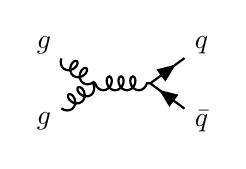
\begin{tikzpicture}[baseline=0, thick]
		\begin{feynman}
			\vertex (i1) at (-\jetdiagw, \jetdiagh) {\(g\)};
			\vertex (i2) at (-\jetdiagw,-\jetdiagh) {\(g\)};
			\vertex (v1) at (-0.35,0);
			\vertex (v2) at ( 0.35,0);
			\vertex (o1) at ( \jetdiagw, \jetdiagh) {\(q\)};
			\vertex (o2) at ( \jetdiagw,-\jetdiagh) {\(\bar{q}\)};
			\diagram* {
				(i1) -- [gluon] (v1),
				(i2) -- [gluon] (v1),
				(v1) -- [gluon] (v2),
				(o2) -- [fermion] (v2) -- [fermion] (o1),
			};
		\end{feynman}
	\end{tikzpicture}%
}

% g g -> q qbar, t-channel quark exchange.
\newcommand{\diagggqqT}{%
	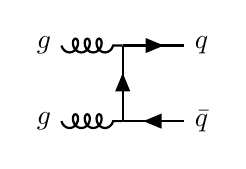
\begin{tikzpicture}[baseline=0, thick]
		\begin{feynman}
			\vertex (i1) at (-\jetdiagw, \jetdiagh) {\(g\)};
			\vertex (i2) at (-\jetdiagw,-\jetdiagh) {\(g\)};
			\vertex (v1) at (0, \jetdiagh);
			\vertex (v2) at (0,-\jetdiagh);
			\vertex (o1) at ( \jetdiagw, \jetdiagh) {\(q\)};
			\vertex (o2) at ( \jetdiagw,-\jetdiagh) {\(\bar{q}\)};
			\diagram* {
				(i1) -- [gluon] (v1),
				(i2) -- [gluon] (v2),
				(o2) -- [fermion] (v2),
				(v2) -- [fermion] (v1),
				(v1) -- [fermion] (o1),
			};
		\end{feynman}
	\end{tikzpicture}%
}

% g g -> q qbar, u-channel: the outgoing quark and antiquark are interchanged.
\newcommand{\diagggqqU}{%
	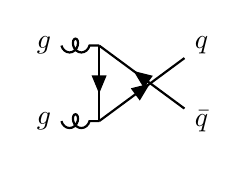
\begin{tikzpicture}[baseline=0, thick]
		\begin{feynman}
			\vertex (i1) at (-\jetdiagw, \jetdiagh) {\(g\)};
			\vertex (i2) at (-\jetdiagw,-\jetdiagh) {\(g\)};
			\vertex (v1) at (-0.30, \jetdiagh);
			\vertex (v2) at (-0.30,-\jetdiagh);
			\vertex (o1) at ( \jetdiagw, \jetdiagh) {\(q\)};
			\vertex (o2) at ( \jetdiagw,-\jetdiagh) {\(\bar{q}\)};
			\diagram* {
				(i1) -- [gluon] (v1),
				(i2) -- [gluon] (v2),
				(o2) -- [fermion] (v1),
				(v1) -- [fermion] (v2),
				(v2) -- [fermion] (o1),
			};
		\end{feynman}
	\end{tikzpicture}%
}

% q g -> q g, s-channel quark exchange.
\newcommand{\diagqgS}{%
	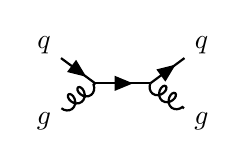
\begin{tikzpicture}[baseline=0, thick]
		\begin{feynman}
			\vertex (i1) at (-\jetdiagw, \jetdiagh) {\(q\)};
			\vertex (i2) at (-\jetdiagw,-\jetdiagh) {\(g\)};
			\vertex (v1) at (-0.35,0);
			\vertex (v2) at ( 0.35,0);
			\vertex (o1) at ( \jetdiagw, \jetdiagh) {\(q\)};
			\vertex (o2) at ( \jetdiagw,-\jetdiagh) {\(g\)};
			\diagram* {
				(i1) -- [fermion] (v1),
				(i2) -- [gluon] (v1),
				(v1) -- [fermion] (v2),
				(v2) -- [fermion] (o1),
				(v2) -- [gluon] (o2),
			};
		\end{feynman}
	\end{tikzpicture}%
}

% q g -> q g, t-channel gluon exchange.
\newcommand{\diagqgT}{%
	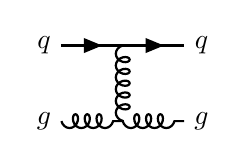
\begin{tikzpicture}[baseline=0, thick]
		\begin{feynman}
			\vertex (v1) at (0, \jetdiagh);
			\vertex (v2) at (0,-\jetdiagh);
			\vertex (i1) at (-\jetdiagw, \jetdiagh) {\(q\)};
			\vertex (o1) at ( \jetdiagw, \jetdiagh) {\(q\)};
			\vertex (i2) at (-\jetdiagw,-\jetdiagh) {\(g\)};
			\vertex (o2) at ( \jetdiagw,-\jetdiagh) {\(g\)};
			\diagram* {
				(i1) -- [fermion] (v1) -- [fermion] (o1),
				(i2) -- [gluon] (v2) -- [gluon] (o2),
				(v1) -- [gluon] (v2),
			};
		\end{feynman}
	\end{tikzpicture}%
}

% q g -> q g, u-channel quark exchange: the outgoing quark and gluon are
% interchanged relative to the t-channel diagram.
\newcommand{\diagqgU}{%
	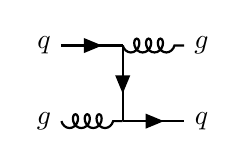
\begin{tikzpicture}[baseline=0, thick]
		\begin{feynman}
			\vertex (v1) at (0, \jetdiagh);
			\vertex (v2) at (0,-\jetdiagh);
			\vertex (i1) at (-\jetdiagw, \jetdiagh) {\(q\)};
			\vertex (o1) at ( \jetdiagw, \jetdiagh) {\(g\)};
			\vertex (i2) at (-\jetdiagw,-\jetdiagh) {\(g\)};
			\vertex (o2) at ( \jetdiagw,-\jetdiagh) {\(q\)};
			\diagram* {
				(i1) -- [fermion] (v1),
				(v1) -- [gluon] (o1),
				(i2) -- [gluon] (v2),
				(v1) -- [fermion] (v2),
				(v2) -- [fermion] (o2),
			};
		\end{feynman}
	\end{tikzpicture}%
}

% q qbar -> g g, s-channel annihilation through the three-gluon vertex.
\newcommand{\diagqqbS}{%
	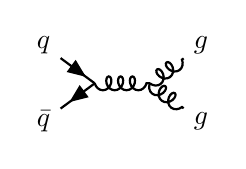
\begin{tikzpicture}[baseline=0, thick]
		\begin{feynman}
			\vertex (i1) at (-\jetdiagw, \jetdiagh) {\(q\)};
			\vertex (i2) at (-\jetdiagw,-\jetdiagh) {\(\bar{q}\)};
			\vertex (v1) at (-0.35,0);
			\vertex (v2) at ( 0.35,0);
			\vertex (o1) at ( \jetdiagw, \jetdiagh) {\(g\)};
			\vertex (o2) at ( \jetdiagw,-\jetdiagh) {\(g\)};
			\diagram* {
				(i1) -- [fermion] (v1) -- [fermion] (i2),
				(v1) -- [gluon] (v2),
				(v2) -- [gluon] (o1),
				(v2) -- [gluon] (o2),
			};
		\end{feynman}
	\end{tikzpicture}%
}

% q qbar -> g g, t-channel quark exchange.
\newcommand{\diagqqbT}{%
	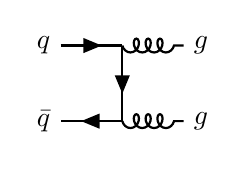
\begin{tikzpicture}[baseline=0, thick]
		\begin{feynman}
			\vertex (i1) at (-\jetdiagw, \jetdiagh) {\(q\)};
			\vertex (i2) at (-\jetdiagw,-\jetdiagh) {\(\bar{q}\)};
			\vertex (v1) at (0, \jetdiagh);
			\vertex (v2) at (0,-\jetdiagh);
			\vertex (o1) at ( \jetdiagw, \jetdiagh) {\(g\)};
			\vertex (o2) at ( \jetdiagw,-\jetdiagh) {\(g\)};
			\diagram* {
				(i1) -- [fermion] (v1),
				(v1) -- [fermion] (v2),
				(v2) -- [fermion] (i2),
				(v1) -- [gluon] (o1),
				(v2) -- [gluon] (o2),
			};
		\end{feynman}
	\end{tikzpicture}%
}

% q qbar -> g g, u-channel: as above with the two outgoing gluons interchanged.
\newcommand{\diagqqbU}{%
	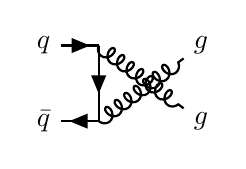
\begin{tikzpicture}[baseline=0, thick]
		\begin{feynman}
			\vertex (i1) at (-\jetdiagw, \jetdiagh) {\(q\)};
			\vertex (i2) at (-\jetdiagw,-\jetdiagh) {\(\bar{q}\)};
			\vertex (v1) at (-0.30, \jetdiagh);
			\vertex (v2) at (-0.30,-\jetdiagh);
			\vertex (o1) at ( \jetdiagw, \jetdiagh) {\(g\)};
			\vertex (o2) at ( \jetdiagw,-\jetdiagh) {\(g\)};
			\diagram* {
				(i1) -- [fermion] (v1),
				(v1) -- [fermion] (v2),
				(v2) -- [fermion] (i2),
				(v1) -- [gluon] (o2),
				(v2) -- [gluon] (o1),
			};
		\end{feynman}
	\end{tikzpicture}%
}

% g g -> g g, s-channel through two three-gluon vertices.
\newcommand{\diagggS}{%
	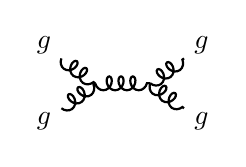
\begin{tikzpicture}[baseline=0, thick]
		\begin{feynman}
			\vertex (i1) at (-\jetdiagw, \jetdiagh) {\(g\)};
			\vertex (i2) at (-\jetdiagw,-\jetdiagh) {\(g\)};
			\vertex (v1) at (-0.35,0);
			\vertex (v2) at ( 0.35,0);
			\vertex (o1) at ( \jetdiagw, \jetdiagh) {\(g\)};
			\vertex (o2) at ( \jetdiagw,-\jetdiagh) {\(g\)};
			\diagram* {
				(i1) -- [gluon] (v1),
				(i2) -- [gluon] (v1),
				(v1) -- [gluon] (v2),
				(v2) -- [gluon] (o1),
				(v2) -- [gluon] (o2),
			};
		\end{feynman}
	\end{tikzpicture}%
}

% g g -> g g, t-channel gluon exchange.
\newcommand{\diagggT}{%
	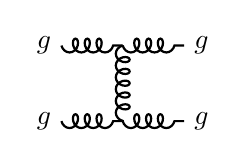
\begin{tikzpicture}[baseline=0, thick]
		\begin{feynman}
			\vertex (v1) at (0, \jetdiagh);
			\vertex (v2) at (0,-\jetdiagh);
			\vertex (i1) at (-\jetdiagw, \jetdiagh) {\(g\)};
			\vertex (o1) at ( \jetdiagw, \jetdiagh) {\(g\)};
			\vertex (i2) at (-\jetdiagw,-\jetdiagh) {\(g\)};
			\vertex (o2) at ( \jetdiagw,-\jetdiagh) {\(g\)};
			\diagram* {
				(i1) -- [gluon] (v1) -- [gluon] (o1),
				(i2) -- [gluon] (v2) -- [gluon] (o2),
				(v1) -- [gluon] (v2),
			};
		\end{feynman}
	\end{tikzpicture}%
}

% g g -> g g, u-channel: the two outgoing gluons are interchanged.
\newcommand{\diagggU}{%
	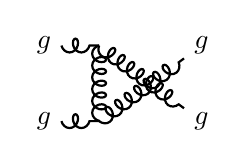
\begin{tikzpicture}[baseline=0, thick]
		\begin{feynman}
			\vertex (v1) at (-0.30, \jetdiagh);
			\vertex (v2) at (-0.30,-\jetdiagh);
			\vertex (i1) at (-\jetdiagw, \jetdiagh) {\(g\)};
			\vertex (o1) at ( \jetdiagw, \jetdiagh) {\(g\)};
			\vertex (i2) at (-\jetdiagw,-\jetdiagh) {\(g\)};
			\vertex (o2) at ( \jetdiagw,-\jetdiagh) {\(g\)};
			\diagram* {
				(i1) -- [gluon] (v1),
				(v1) -- [gluon] (o2),
				(i2) -- [gluon] (v2),
				(v2) -- [gluon] (o1),
				(v1) -- [gluon] (v2),
			};
		\end{feynman}
	\end{tikzpicture}%
}

% g g -> g g, the four-gluon contact term (cf. the four-gluon vertex of
% tab:qcdrules), redrawn here on the common 2->2 scale.
\newcommand{\diagggX}{%
	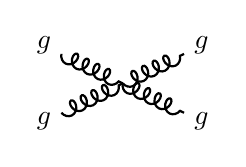
\begin{tikzpicture}[baseline=0, thick]
		\begin{feynman}
			\vertex (v) at (0,0);
			\vertex (i1) at (-\jetdiagw, \jetdiagh) {\(g\)};
			\vertex (i2) at (-\jetdiagw,-\jetdiagh) {\(g\)};
			\vertex (o1) at ( \jetdiagw, \jetdiagh) {\(g\)};
			\vertex (o2) at ( \jetdiagw,-\jetdiagh) {\(g\)};
			\diagram* {
				(i1) -- [gluon] (v),
				(i2) -- [gluon] (v),
				(v) -- [gluon] (o1),
				(v) -- [gluon] (o2),
			};
		\end{feynman}
	\end{tikzpicture}%
}

% Macro for 4-point vertices
% Args: #1=top-left style, #2=top-left label, #3=bottom-left style, #4=bottom-left label,
%       #5=top-right style, #6=top-right label, #7=bottom-right style, #8=bottom-right label
\newcommand{\fourvertex}[8]{%
	\begin{tikzpicture}[baseline=0, thick]
		\begin{feynman}
			\vertex [circle, fill=black, minimum size=3.5pt, inner sep=0pt] (v) at (0,0) {};
			\vertex (i1) at (135:1.5) {\(#2\)};
			\vertex (i2) at (225:1.5) {\(#4\)};
			\vertex (o1) at (45:1.5) {\(#6\)};
			\vertex (o2) at (-45:1.5) {\(#8\)};
			\diagram* {
				(i1) -- [#1] (v),
				(i2) -- [#3] (v),
				(v) -- [#5] (o1),
				(v) -- [#7] (o2),
			};
		\end{feynman}
	\end{tikzpicture}%
}

\def\splitw{0.95} % half-width  of a 1->2 splitting diagram
\def\splith{0.62} % half-height of a 1->2 splitting diagram
\newcommand{\splitvertex}[9]{%
	\begin{tikzpicture}[baseline=0, thick]
		\begin{feynman}
			\vertex [circle, fill=black, minimum size=3.5pt, inner sep=0pt] (v) at (0,0) {};
			\vertex (p) at (-\splitw, 0)        {\(#2\)};
			\vertex (u) at ( \splitw,  \splith) {\(#5\)};
			\vertex (l) at ( \splitw, -\splith) {\(#8\)};
			\diagram* {
				(p) -- [#1, edge label'=\(#3\)] (v),
				(v) -- [#4, edge label=\(#6\)]  (u),
				(v) -- [#7, edge label'=\(#9\)] (l),
			};
		\end{feynman}
	\end{tikzpicture}%
}
% Devanagari words: XeLaTeX-typeset PDFs (figures/devanagari/make_devanagari.py) placed on the
% baseline, with the Unicode text attached as ActualText so they copy and search as text.
\usepackage{accsupp}
% Generated by figures/devanagari/make_devanagari.py -- do not edit.
\expandafter\def\csname devhex@vaisesikasutra\endcsname{09350948093609470937093F09150020093809420924094D0930}% वैशेषिक सूत्र
\expandafter\def\csname devhex@anu\endcsname{090509230941}% अणु
\expandafter\def\csname devhex@paramanu\endcsname{092A0930092E093E09230941}% परमाणु
\expandafter\def\csname devhex@dharma\endcsname{09270930094D092E}% धर्म
\expandafter\def\csname devhex@moksha\endcsname{092E094B0915094D0937}% मोक्ष
\expandafter\def\csname devhex@nirvana\endcsname{0928093F0930094D0935093E0923}% निर्वाण

\makeatletter
\newcommand{\devword}[1]{%
	\edef\dev@act{\noexpand\BeginAccSupp{method=hex,unicode,ActualText=\csname devhex@#1\endcsname}}%
	\dev@act\raisebox{-0.3em}{\includegraphics[height=1.35em]{figures/devanagari/#1.pdf}}\EndAccSupp{}}
\makeatother

% clickable citations, cross-references, table of contents and URLs (keep hyperref last)
\usepackage[hyperfootnotes=false]{hyperref}
\hypersetup{
	colorlinks=true,
	linkcolor=blue!50!black,
	citecolor=blue!50!black,
	urlcolor=blue!50!black,
	bookmarksnumbered=true,
	pdftitle={Spacetime evolution of jets with the STAR experiment},
	pdfauthor={Tanmay Pani},
}

\newenvironment{itquote}
{\begin{quote}\itshape}
{\end{quote}\ignorespacesafterend}
	
\begin{document}
\phd \title{Spacetime evolution of jets with the STAR experiment}
\author{Tanmay Pani}
\program{Physics and Astronomy}
\director{Prof. Sevil Salur}
\approvals{5}
\submissionyear{2026}
\submissionmonth{September}

\abstract{
%
Most of the stable matter in the universe is made of protons and neutrons, bound in atomic nuclei.
%
Protons and neutrons, or hadrons, are themselves composite objects made of quarks and gluons, or partons, which are, as far as we know, the fundamental particles of the strong nuclear force.
%
Quantum Chromodynamics (QCD), the field theory of the strong force, confines partons inside hadrons under ``normal'' circumstances.
%
However, when matter is heated to extremely high temperatures or compressed to extremely high densities, QCD predicts a transition from hadronic matter into a state of deconfined quarks and gluons, the Quark-Gluon Plasma (QGP).

The QGP is created in the laboratory by colliding nuclei at nearly the speed of light.
%
In the earliest stage of these collisions, before the QGP forms, partons scatter with large momentum transfers.
%
In vacuum, the scattered partons radiate and fragment into collimated sprays of hadrons called jets.
%
In heavy-ion collisions, they must first traverse the QGP and lose energy through collisional and radiative interactions with it, which modifies the resulting jets compared to proton-proton (\(p+p\)) collisions.
%
This phenomenon, jet quenching, is a primary probe of the QGP.

This thesis presents two jet measurements with the STAR experiment at RHIC.
%
The first measures the distributions of charged hadrons around jets in 20--50\% central Au+Au collisions at \sNN{200}{GeV}, separately for jets oriented in, between and out of the event plane, to test whether jet quenching depends on the path length through the QGP.
%
Within the experimental uncertainties, the associated yields and the widths of the jet peaks show no dependence on the event plane.

The second characterizes the angular spread of energy inside jets with generalized angularities, corrected for detector effects with unbinned, machine-learning based unfolding.
%
In Au+Au collisions, the angularities of jets with hard constituents are consistent between central and peripheral collisions, in the first heavy-ion application of this unfolding technique.
%
In \(p+p\) collisions at \sPP{200}{GeV}, the inclusive and SoftDrop-groomed angularities of inclusive jets are measured as a baseline for future heavy-ion measurements.
%
The jets become narrower with increasing jet momentum and with grooming, and the event generators PYTHIA\mbox{-}8 and HERWIG\mbox{-}7 predict narrower jets than measured.
%
Measuring the mean angularities as functions of the groomed jet radius, which the unbinned unfolding makes possible, shows that these generators produce too little radiation at a given splitting angle.
}

\beforepreface

\acknowledgements{
As I am writing this thesis, Christopher Nolan's blockbuster movie, ``The Odyssey'' has brought Homer's 2800-year-old epic back into the forefront of cultural conversation. 
%
Perhaps it is fitting that I bring my graduate school journey to an end, thinking of Odysseus's voyage home.
%
While not quite as perilous as the complicated hero's journey, I would not say it was easy.
%
Even though I didn't have to sail through the choppy waters between Scylla and Charybdis, I did have to take a 14-hour flight across the Atlantic on 30 August 2020 during the peak of the COVID pandemic. 
%
My penchant for getting waylaid from my course (of research) definitely rivals that of the men from Ithaca.
%
However, all through it, much like Athena with Odysseus, Prof. Sevil Salur was always looking out for me. 
%

Characters in Homer's epics often talk about \emph{xenia}, the ancient Greek tradition of hospitality to strangers, of giving them the benefit of the doubt. 
%
I believed I lived in a world where xenia was long dead, but my committee, Prof. Matthew R. Buckley, Prof. John P. Hughes, Prof. Ronald D. Ransome and Dr. Isaac A. Mooney have made me rethink that position. 
%
Without their support and belief in my work, this thesis would not have been submitted.

At the edge of the underworld, the shade of the Theban seer Tiresias told Odysseus to carry an oar inland until he met people who did not know what an oar was, to make his peace with Poseidon there, and only then to go home to a quiet old age.
%
The Odyssey ends before that part of the story, but wherever I have to carry my own oar next, I know where home is: with my wife, the love of my life, Dr. Claire L. Riggs.

Like Argos, who waited twenty years for Odysseus to come home, my cats, Janeway and Bones, were waiting at the end of every long day. Janeway, named after the Star Trek captain who spent seven years finding her way home, supported me through all of it, asking only to be brushed in return, and Bones, named after the Enterprise's doctor, prescribed purrs for every bad day, payable in treats.

Fortunately, the merry cast of people whose help and support was invaluable to me are doing alright and not eaten by Cyclopses, morphed into swine by Circe or drowned by Poseidon. 
%
Thus, I will stop drawing analogies with Odysseus's voyage and go to the story of Aeneas, the heroic Trojan from The Iliad, whose difficult journey to Italy Virgil told about 700 years after Homer, in the Aeneid. 
%
Much like Achates to Aeneas, for over a decade Dr. Diptanil Roy has been a friend I could rely on during good and bad times. 
%
And like the Sibyl of Cumae who led Aeneas through the underworld, Dr. Joel A. Mazer guided me through the depths of the jet-hadron analysis.
%
Like Mercury, sent by Jupiter to ensure a warm welcome for the shipwrecked Trojans in Carthage, Prof. Ronald Gilman and Shirley Hinds smoothed my way through the paperwork of graduate school.
%
My other shipmates, colleagues from Sevil's group, Khovesh Ramdin, Ravi Koka and Jinglin Liu, kept the oars moving through the calm and the storms alike, and made the long voyage feel much shorter than it was.

Here I leave the epics behind.
%
Their heroes had gods to guide them and poets to remember them, but at the end of the day they were never human in the way I am, and what carried me through was far more ordinary, and far more precious: my family.
%
My parents, Lingaraj Pani and Sharmila Dash, gave me every resource I needed to grow, and defied every social norm that could have stood in the way of my education.
%
My sister, Auroshree Pani, was born when I was five and became my first friend.
%
I am very fortunate that she flew to the US with me in 2020 to begin her undergraduate studies, so that I still get to be part of the family I grew up with from time to time.

To all named here, and the many others who helped along the way, thank you. \emph{Forsan et haec olim meminisse iuvabit}\footnote{Virgil, \emph{Aeneid} 1.203, Aeneas to his crew after the storm.}, perhaps one day it will be a joy to remember even this.

}

\dedication{
	\begin{center}
		{\em To family, for what else is there?} \\
		{\em And to the family yet to come, who will take my oar for a winnowing fan.} \\
	\end{center}
}

\figurespage
\tablespage

\afterpreface
\graphicspath{{./}{figures/}}
% \def\figdirgap{./Figures/Gappies}
% \def\figdirudg{./Figures/UDGs}
% \def\figdirlsb{./Figures/LSBs}
% \captionsetup{font={stretch=1}} 

\chapter{Introduction}
\label{ch:intro}
Since ancient times, humans have pondered the nature of matter, as evidenced by the fact that between 2000-3000 years ago, the Greeks and Indians independently developed the philosophical school of \emph{Atomism}. 
%
The words ``atomism'' and  ``atoms'' are etymologically linked to the Greek word \emph{atomon} (indivisible), first used by Democritus in 500 B.C., to denote the most fundamental, indivisible unit of matter~\cite{taylor1999atomists}. 
%
The atomon of Democritus differed from the matter they came from quantitatively but not qualitatively (an atom of wood would still be an almost infinitesimal piece of wood). 
%
Later around 340-330 B.C., Aristotle's \emph{hylomorphic} (from Greek words \emph{hyle} for matter and \emph{morphe} for form) worldview challenged Democritus's assumption of the atomon's indivisibility, as it was simply not verifiable in ancient Greece~\cite{Lloyd1970EarlyGreekScience}. 
%
The ingenuity of Aristotle's hylomorphism lay in his abstraction of the unknown, he theorized the \emph{elachista} (Greek word for minima, later translated into Latin as \emph{minima naturalia})  not as an indivisible unit of matter,  but simply a \emph{size scale} beyond which matter could no longer be structured into recognizable forms like flesh, wood, bronze, etc.


Meanwhile, sometime between 600-200 B.C., the Indian philosopher Kanada developed a non-theistic, atomistic approach to the Vedas in the Sanskrit text \emph{Vaishesika Sutra} (Sanskrit: \devword{vaisesikasutra}, IAST: \emph{Vai\'se\d{s}ika S\=utra}, lit.\ `aphorisms on particularity')~\cite{chakrabarty2003vaisesika}.
%
Kanada postulated that even the smallest division of any material that still resembles the matter, \emph{Anu} (Sanskrit: \devword{anu}, IAST: \emph{a\d{n}u}, lit.\ `atom') would further comprise of \emph{Paramanu} (Sanskrit: \devword{paramanu}, IAST: \emph{param\=a\d{n}u}, lit.\ `ultimate atom').
%
Interestingly, Kanada's paramanu were qualitatively different than ordinary matter and were of four kinds, two with mass and two without, and their indivisibility came from their immeasurability, making his theories resemble a middle ground between Aristotle and Democritus.
%
Kanada also went into concepts like rotational invariance (the paramanu must be spherical to be the same from all directions).
%
However, even though the words Anu and Paramanu are still used to mean ``atom'' and ``nuclear/sub-atom'' respectively in almost every language spoken in today's India, the ultimate objective of Kanada's sutras had little to do with formalizing natural phenomena and were mostly a metaphysical reading of Vedic teachings like \emph{Dharma} (Sanskrit: \devword{dharma}, IAST: \emph{dharma}) and \emph{Moksha} (Sanskrit: \devword{moksha}, IAST: \emph{mok\d{s}a}, lit.\ `liberation'), the Vedic counterpart of the Buddhist \emph{Nirvana} (Sanskrit: \devword{nirvana}, IAST: \emph{nirv\=a\d{n}a}, lit.\ `blowing out')~\cite{klostermaier2010survey}.  
%

Around 2000 years later, Aristotle's minima naturalia became the foundation of \emph{corpuscular theories} from European natural philosophers like Isaac Newton, Ren\'e Descartes and Robert Boyle. 
%
Particularly, in 1704 Isaac Newton's \emph{Opticks}~\cite{Newton:1704} described the \emph{Corpuscular theory of light}, conceptualizing light as a rectilinear stream of discrete ``corpuscles''  with a finite velocity, an early version of the modern \emph{photons}.
%
With the perfected versions of Newton's optics explaining phenomena like reflection, refraction, polarization, etc. the corpuscular school of thought was dominant in scientific circles of 18th century Europe.  
%
Although Thomas Young and his double-slit experiment in 1801~\cite{Young:1804} ousted the corpuscular theory of light from annals of serious scientific discourse for rest of 19th century, the resurrection of atomism as a serious scientific philosophy was already being scripted in John Dalton's notebooks. 
%
Between 1803 and 1808, Dalton proposed that every chemical element consists of identical, indivisible atoms that combine in fixed, whole-number ratios, explaining the laws of chemical combination and turning atomism into a quantitative, testable theory~\cite{Dalton:1808}.

The indivisibility of Dalton's atoms lasted less than a century.
%
In 1897, J.J. Thomson showed that cathode rays are made of negatively charged particles far lighter than any atom, the \emph{electron}, the first fundamental particle to be discovered and the first sign that atoms have an internal structure~\cite{Thomson:1897}.
%
Soon after, Planck (1900) and Einstein (1905) revived Newton's corpuscles in a new form: light is emitted and absorbed in discrete quanta, later called \emph{photons}~\cite{Planck:1901,Einstein:1905}.
%
In 1911, Rutherford's analysis of alpha particles scattered off a thin gold foil revealed that almost all the mass of an atom is concentrated in a tiny, positively charged \emph{nucleus}~\cite{Rutherford:1911}, which by 1932 was known to consist of \emph{protons} (Rutherford, 1919)~\cite{Rutherford:1919} and \emph{neutrons} (Chadwick, 1932)~\cite{Chadwick:1932}.
%
In 1928, Dirac's relativistic equation for the electron predicted antimatter~\cite{Dirac:1928}, and its first example, the \emph{positron}, was found by Anderson in cosmic rays in 1932~\cite{Anderson:1933}.
%
The following decades brought a flood of unexpected particles, the \emph{muon}~\cite{Neddermeyer:1937}, the \emph{pion}~\cite{Lattes:1947}, the \emph{strange} particles~\cite{Rochester:1947} and the \emph{neutrino}~\cite{Cowan:1956}, and, with the new accelerators of the 1950s, dozens of short-lived hadrons, a ``particle zoo'' too large to be fundamental.

Order was restored in 1964, when Gell-Mann and Zweig proposed that hadrons are built from a few \emph{quarks}~\cite{GellMann:1964,Zweig:1964}, which soon had to be given a new quantum number, \emph{color}~\cite{Greenberg:1964,HanNambu:1965}.
%
The deep-inelastic scattering experiments at SLAC in 1968--1969, in a sense Rutherford's experiment repeated at a much finer scale, found that the proton indeed contains point-like constituents, the \emph{partons}, later identified with quarks~\cite{Bloom:1969,Breidenbach:1969}.
%
In 1973, Gross, Wilczek and Politzer showed that a non-Abelian gauge theory of color, \emph{Quantum Chromodynamics} (QCD), is asymptotically free, i.e.\ its coupling becomes weak at short distances, making QCD the theory of the strong interaction~\cite{PhysRevLett.30.1343,PhysRevLett.30.1346}.
%
Between 1974 and 1977, the discoveries of the \emph{charm} quark (through the J/\(\psi\)), the \emph{tau} lepton and the \emph{bottom} quark hinted at a third generation of matter~\cite{Aubert:1974,Augustin:1974,Perl:1975,Herb:1977}.
%
Quarks and gluons themselves are never observed in isolation, but their traces are: two collimated sprays of hadrons, \emph{jets}, were seen in electron-positron annihilation at SLAC in 1975~\cite{Hanson:1975}, and the three-jet events observed at the PETRA collider at DESY in 1979 were the first direct evidence of the \emph{gluon}~\cite{TASSO:1979}.
%
The \emph{W} and \emph{Z} bosons of the unified electroweak theory were discovered at CERN in 1983~\cite{UA1W:1983,UA2W:1983,UA1Z:1983}, the \emph{top} quark at Fermilab in 1995~\cite{CDFtop:1995,D0top:1995} and the \emph{tau neutrino} in 2000~\cite{DONUT:2001}, completing three generations of quarks and leptons.
%
Finally, the discovery of the \emph{Higgs boson} at CERN in 2012~\cite{ATLASHiggs:2012,CMSHiggs:2012} completed the particle content of the Standard Model, described in the following section.


%===========================================================================================
%\section{History}
%===========================================================================================
%\subsection{Atomism}
%===========================================================================================
\section{The Standard Model}
According to the Standard Model (SM), all matter results from interactions between fundamental particles: lepton and quarks (fermions), and mediators (bosons).
Tab.~\ref{tab:qrknlep} shows fermions of the standard model, their anti-particle equivalent would have all the signs reversed for the quantum numbers. For example, an anti-electron (\(e^+\)) and anti-electron-neutrino (\(\bar{\nu_e}\)) lepton number would flip to \((-1, 0, 0)\) and charges (\(Q\)s) would be \(+1\) and 0 respectively.

\begin{table}
	\centering
	\begin{tabular}{c @{\hspace{5pt}} l |c|c|c|l|c|c|c|}
		% Top edges of both tables
		\cline{3-5} \cline{7-9}
		
		% Table Headers (overriding borders explicitly to ensure the outer walls exist)
		\multicolumn{2}{c|}{}              & \multicolumn{3}{c|}{Leptons} &              & \multicolumn{3}{c|}{Quarks}                                                                                         \\
		\cline{3-5} \cline{7-9}
		
		% Column Headers (merging the first two columns to center 'Category' with no borders)
		&                              & \(l\)        & \(Q\)                       & \((L_e, L_\mu, L_\tau)\) &  & \(q\) & \(Q\)      & \((F_d, F_u, F_s, F_c, F_b, F_t)\) \\
		\cline{3-5} \cline{7-9}
		
		% Group A block
		\multirow{2}{*}{First generation}  & \ldelim\{{2}{*}              & \(e^-\)      & \(-1\)                      & (1, 0, 0)                &  & \(d\) & \(-1/3\)   & \((-1, 0, 0, 0, 0, 0)\)            \\
		&                              & \(\nu_e\)    & 0                           & (1, 0, 0)                &  & \(u\) & \(2/3\)    & \((0, 1, 0, 0, 0, 0)\)             \\
		\cline{3-5} \cline{7-9}
		
		% Group B block
		\multirow{2}{*}{Second generation} & \ldelim\{{2}{*}              & \(\mu^-\)    & \(-1\)                      & (0, 1, 0)                &  & \(s\) & \( -1/3 \) & \((0, 0, -1, 0, 0, 0)\)            \\
		&                              & \(\nu_\mu\)  & 0                           & (0, 1, 0)                &  & \(c\) & \(2/3\)    & \((0, 0, 0, 1, 0, 0)\)             \\
		\cline{3-5} \cline{7-9}
		
		% Group B block
		\multirow{2}{*}{Third generation}  & \ldelim\{{2}{*}              & \(\tau^-\)   & \(-1\)                      & (0, 0, 1)                &  & \(b\) & \(-1/3\)   & \((0, 0, 0, 0, -1, 0)\)            \\
		&                              & \(\nu_\tau\) & 0                           & (0, 0, 1)                &  & \(t\) & \(2/3\)    & \((0, 0, 0, 0, 0, 1)\)             \\
		% Bottom edges of both tables                         
		\cline{3-5} \cline{7-9}
	\end{tabular}
	\caption{Three generations of leptons (left) and quarks (right).}
	\label{tab:qrknlep}
\end{table}

\begin{figure}
	\begin{tabular}{
			>{\centering\arraybackslash}m{2.8cm}
			>{\centering\arraybackslash}m{2.8cm}
			>{\centering\arraybackslash}m{2.8cm}
			>{\centering\arraybackslash}m{2.8cm}
		}
		
		% ROW 1: Strong Vertices
		\multicolumn{1}{c}{\vhead{Electromagnetic} }                                                      & \multicolumn{3}{l}{\vhead{Strong}} \\[0.1cm]
		\threevertex{fermion}{X^{+|-}}{fermion}{X^{-|+}}{photon}{\gamma}                                  &
		\threevertex{fermion}{q}{fermion}{q}{gluon}{g}                                                    &
		\threevertex{gluon}{g}{gluon}{g}{gluon}{g}                                                        &
		\fourvertex{gluon}{g}{gluon}{g}{gluon}{g}{gluon}{g}
		\\[1cm]
		
		% ROW 3: Electromagnetic and Electroweak Vertices
		\multicolumn{3}{l}{\vhead{Weak}}                                                                  &                                    \\[0.1cm]
		\threevertex{fermion}{\nu_e \mid \nu_\mu \mid \nu_\tau}{fermion}{e \mid \mu \mid \tau}{photon}{W} &
		\threevertex{fermion}{d/s/b}{fermion}{u/c/t}{photon}{W}                                           &
		\threevertex{fermion}{f}{fermion}{f}{photon}{Z}                                                   &
		
		
		
		\\[1cm]
		\multicolumn{2}{l}{\vhead{Electroweak}}                                                           & \multicolumn{2}{l}{\vhead{Higgs}}  \\[0.1cm]
		\threevertex{photon}{Z/\gamma}{photon}{W}{photon}{W}                                              &
		\fourvertex{photon}{W}{photon}{W}{photon}{W|Z/\gamma}{photon}{W|Z/\gamma}                         &
		\threevertex{fermion}{m}{fermion}{m}{scalar}{H}                                                   &
		\fourvertex{scalar}{H}{scalar}{H}{scalar}{m_B}{scalar}{m_B}
	\end{tabular}
	\caption[Feynman diagrams of the interaction vertices of the Standard Model]{Feynman diagrams of the interaction vertices of the Standard Model. \(X^{+|-}\), \(X^{-|+}\): an electrically charged fermion and its antiparticle; \(q\): quark; \(g\): gluon; \(\gamma\): photon; \(\nu_e, \nu_\mu, \nu_\tau\): neutrinos; \(e, \mu, \tau\): charged leptons, of the same flavor as the neutrino at the vertex; \(u/c/t\): up, charm, top quarks; \(d/s/b\): down, strange, bottom quarks; \(f\): any fermion; \(W\), \(Z\): weak gauge bosons; \(H\): Higgs boson; \(m\): any massive fermion; \(m_B\): any massive boson (\(H\), \(W\) or \(Z\)). A vertical bar or slash separates alternatives, e.g.\ \(W|Z/\gamma\) stands for a \(W\), \(Z\) or \(\gamma\).}
	\label{fig:smvtx}
\end{figure}

The mediators/bosons exchanged between the other fundamental particles give rise to the fundamental interactions: electromagnetism from the photon (\(\gamma\)), weak force from \(W^\pm\) and \(Z\) bosons, the gluon (\(g\)) for the strong force, and the Higgs boson (\(h\)) for imparting mass to the fundamental particles. Various interaction vertices possible in SM, that become the building blocks of all fundamental interactions are shown in Fig.~\ref{fig:smvtx}.
%
The figure groups them by interaction: the photon couples to every electrically charged fermion, the gluon to quarks and to itself through the three- and four-gluon vertices, the \(W\) to a charged lepton and its neutrino or to an up-type and a down-type quark, and the \(Z\) to any fermion pair, while the electroweak and Higgs vertices couple the gauge bosons to each other and the Higgs boson to the massive particles.

Each vertex in Fig.~\ref{fig:smvtx} is a point where a mediator is emitted or absorbed, and its strength is set by the \emph{coupling} of the corresponding interaction: the electric charge \(e\) for the photon, the weak couplings for the \(W^\pm\) and \(Z\), and the strong coupling \(g_s\) for the gluon.
%
Every vertex in a Feynman diagram contributes one factor of its coupling to the quantum-mechanical amplitude of a process, and the cross section, being proportional to the square of the amplitude, therefore scales as a power of the dimensionless combinations \(\alpha = e^2/4\pi \approx 1/137\) and \(\alpha_s = g_s^2/4\pi\).
%
For example, the scattering of two quarks by the exchange of a gluon, or the annihilation of a quark and an antiquark into a gluon that produces a new pair (Fig.~\ref{fig:qqScattering}), has two vertices, so its amplitude is proportional to \(g_s^2\) and its cross section to \(\alpha_s^2\).
%
Any additional emission, or any virtual loop, adds more vertices and hence more powers of the coupling, so the prediction for a process takes the form of a series in \(\alpha\) or \(\alpha_s\).
%
Such a \emph{perturbative} expansion is only useful when the coupling is small, which is well satisfied for electromagnetism.
%
As discussed in Sec.~\ref{subsec:runningCoupling}, the couplings are not constants but depend on the momentum transfer \(Q\) of the interaction, and for the strong interaction this dependence decides where perturbation theory can be used at all.

\begin{figure}[htbp]
	\centering
	\begin{tabular}{c@{\hspace{2cm}}c}
		\diagqqpT{q'}{q} & \diagqqbAnn{q}{q'} \\[0.3cm]
		(a) & (b)
	\end{tabular}
	\caption{Leading-order Feynman diagrams of (a) the scattering of two quarks, \(qq' \to qq'\), by the exchange of a gluon, and (b) the annihilation of a quark and an antiquark into a gluon that produces a new pair, \(q\bar{q} \to q'\bar{q}'\). Both contain two quark-gluon vertices of Fig.~\ref{fig:smvtx}, so their amplitudes are proportional to \(g_s^2\) and their cross sections to \(\alpha_s^2\).}
	\label{fig:qqScattering}
\end{figure}


%===========================================================================================
\section{Quantum Chromodynamics}
\label{sec:QCDIntro}

\emph{Quantum Chromodynamics (QCD)} is the component of the SM that describes the strong interaction of quarks and gluons, collectively called \emph{partons}.
%
Its charge, the analogue of the electric charge of quantum electrodynamics (QED), is called \emph{color}: every quark carries one of three colors, conventionally named red (\(r\)), green (\(g\)) and blue (\(b\)), and every antiquark one of the three anticolors (\(\bar{r}\), \(\bar{g}\), \(\bar{b}\)).

The names of the colors are arbitrary, and physics must not change if the three color states of a quark are relabeled.
%
More generally, it must not change if they are \emph{shuffled}, i.e.\ mixed into each other, \(r \to \cos\theta\,r + \sin\theta\,g\) and \(g \to -\sin\theta\,r + \cos\theta\,g\) being one example.
%
Any such shuffle that preserves the total probability is a \(3\times3\) unitary matrix acting on the column \((r, g, b)\), and those with unit determinant form the group \(\mathrm{SU}(3)\).
%
In QED, the only corresponding freedom is a change of the overall complex phase of the electron field, which forms the group \(\mathrm{U}(1)\).
%
QCD requires this freedom locally: the colors may be shuffled differently at every point in space and time.
%
Two neighboring quarks can then only be compared if there is a field that relates their color frames, and this field is the \emph{gluon}.
%
There is one gluon for every independent infinitesimal shuffle, of which \(\mathrm{SU}(3)\) has \(3^2 - 1 = 8\), so there are eight gluons, while \(\mathrm{U}(1)\) has a single one, the photon.

When a quark emits or absorbs a gluon, its color changes: a red quark turning green emits a gluon that carries away red and brings in green, i.e.\ a red-antigreen (\(r\bar{g}\)) gluon.
%
Gluons therefore carry a color and an anticolor.
%
Of the \(3 \times 3 = 9\) color-anticolor combinations, the one that is completely symmetric in the three colors, \((r\bar{r} + g\bar{g} + b\bar{b})/\sqrt{3}\), is unchanged by every shuffle.
%
It is a \emph{color singlet}, carries no net color and does not take part in the strong interaction, leaving eight gluons, as found above (in group-theory notation, \(\mathbf{3}\otimes\bar{\mathbf{3}} = \mathbf{8}\oplus\mathbf{1}\)).
%
Only color singlets are observed in nature: the \emph{mesons}, quark-antiquark pairs in exactly this symmetric combination, and the \emph{baryons}, three quarks in the combination that is antisymmetric in color, such as the proton and the neutron.

Successive shuffles do not commute: mixing \(r\) with \(g\) and then \(g\) with \(b\) gives a different result than doing the same in the opposite order, just as two rotations about different axes in space do.
%
\(\mathrm{SU}(3)\) is therefore a \emph{non-Abelian} group, unlike the Abelian \(\mathrm{U}(1)\) of QED.
%
Because gluons are themselves colored, a shuffle of the colors also rotates the gluons, and gluons consequently interact with other gluons.
%
This is the origin of the three- and four-gluon vertices of Fig.~\ref{fig:smvtx}, which have no counterpart for the electrically neutral photon.
%
The corresponding Lagrangian and Feynman rules are given in App.~\ref{sec:qcdLagrangian}.

The strength with which a parton radiates gluons is set by its color charge, quantified by the \emph{color factors} \(C_F = 4/3\) for quarks and \(C_A = 3\) for gluons.
%
A gluon therefore radiates about \(C_A/C_F = 9/4\) times more than a quark, so jets initiated by gluons contain more, and more widely spread, radiation than those initiated by quarks.



\subsection{The Running Coupling}
\label{subsec:runningCoupling}

\begin{figure}
	\centering
	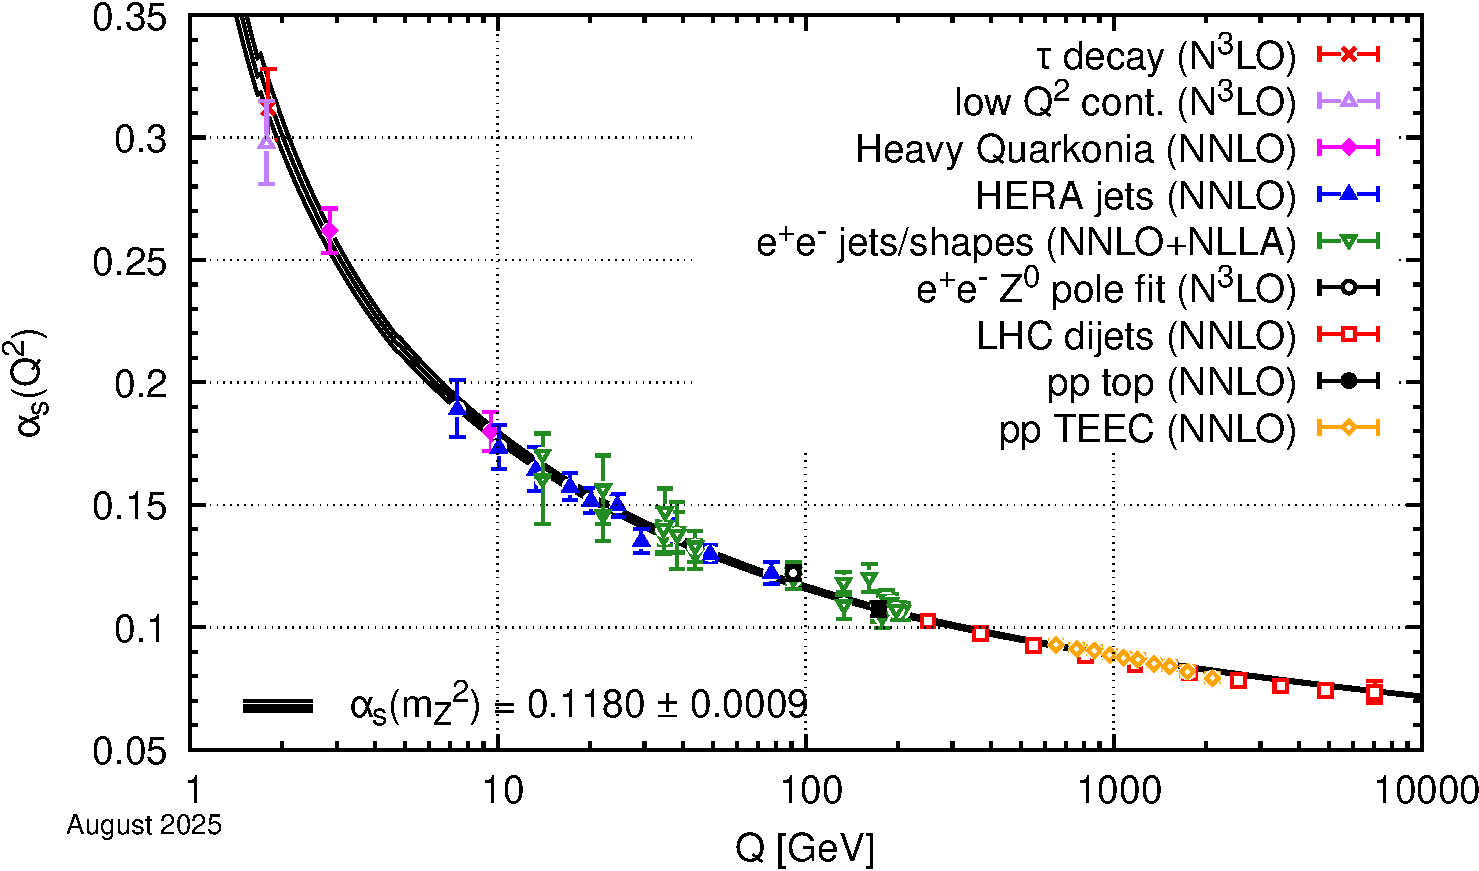
\includegraphics[width=0.7\linewidth]{figures/alphas-v-Q-2025-cropped.pdf}
	\caption{Summary of determinations of \(\alpha_s\) as a function of the energy scale Q compared to
		the running of the coupling computed at five loops taking as an input the current Particle Data Group (PDG) world average, \(\alpha_s(m_Z^2) = 0.1180 \pm 0.0009\)~\cite{ParticleDataGroup:2026aaa}.}
	\label{fig:runningCoupling}
\end{figure}

The coupling of a vertex in Fig.~\ref{fig:smvtx} is not a fixed number, because virtual loops around the vertex change the charge seen by a probe at a given momentum transfer \(Q\)~\cite{peskin2018introduction}.
%
In QED, virtual electron-positron pairs polarize the vacuum and \emph{screen} the electric charge, so that \(\alpha\) grows slowly with \(Q\), from about \(1/137\) at low \(Q\) to about \(1/128\) at the mass of the \(Z\) boson~\cite{ParticleDataGroup:2026aaa}.
%
In QCD, virtual quark-antiquark pairs screen the color charge in the same way, but the colored gluons around a charge have the opposite effect and \emph{anti-screen} it~\cite{PhysRevLett.30.1343,PhysRevLett.30.1346}.
%
Anti-screening wins as long as there are fewer than 17 quark flavors, so \(\alpha_s\) decreases with \(Q\).
%
At leading order~\cite{ParticleDataGroup:2026aaa},
\begin{equation}
	\alpha_s(Q^2) = \frac{\alpha_s(Q_0^2)}{1 + \beta_0\,\alpha_s(Q_0^2)\ln(Q^2/Q_0^2)}, \qquad \beta_0 = \frac{11 C_A - 2 n_f}{12\pi},
	\label{eq:alphasVsQ2}
\end{equation}

%At an energy scale \(Q\), consider a dimensionless observable \(X\). Lets assume that \(Q\) is sufficiently high that the quark masses become negligible in comparison. To calculate \(X\) as a perturbation series in the QCD coupling \(\alpha_s = \frac{g^2}{4\pi}\) (analogous to the QED fine structure constant), we need to remove ultraviolet divergences through renormalization. Renormalization introduces another arbitrary energy scale $\mu$ where the divergences are subtracted.  In general, \(X\) would depend on the ratio \(Q^2/\mu^2\) and post-renormalization coupling $\alpha_s(\mu^2)$. However, any physical observable should be independent of $\mu$:
%\begin{align}
%	\mu^2\frac{d X(Q^2/\mu^2, \alpha_s(\mu^2))}{d\mu^2} &= \left[\mu^2\frac{\partial}{\partial\mu^2} +  \mu^2\frac{\partial\alpha_s(\mu^2)}{\partial\mu^2}\frac{\partial}{\partial\alpha_s}\right] X(Q^2/\mu^2, \alpha_s(\mu^2)) = 0 \notag\\
%	\implies & \left[-\frac{\partial}{\partial t} + \beta(\alpha_s) \frac{\partial}{\partial\alpha_s}\right] X(e^t, \alpha_s) = 0.
%	\label{eqn:renormX}
%\end{align} 
%
%Where, \(t = \ln{\frac{Q^2}{\mu^2}}\), \(\beta(\alpha_s) = \mu^2\frac{\partial\alpha_s}{\partial\mu^2}\), \(\alpha_s\equiv\alpha_s(\mu^2(t))\)
%\begin{align}
%	\beta(\alpha_s) &= -\frac{\partial\alpha_s}{\partial t} \implies  t =  \int^{\alpha_s(Q^2)}_{\alpha_s}\frac{d\alpha_s}{\beta(\alpha_s)}\notag\\
%	\implies & \frac{\partial\alpha_s(Q^2)}{\partial t} = Q^2\frac{\partial \alpha_s}{\partial Q^2}  =  \beta(\alpha_s(Q^2)), \quad\frac{\partial\alpha_s(Q^2)}{\partial\alpha_s} = \frac{\beta(\alpha_s(Q^2))}{\beta(\alpha_s)}
%	\label{eq:runningCouplingIntro}
%\end{align}
%
%Substituting in Eq.~\ref{eqn:renormX}, we see that \(X(1, \alpha_s(Q^2))\) is a valid solution. Thus the scale dependence in \(X\) comes from the \emph{running coupling} \(\alpha_s(Q^2)\).  Perturbatively expanding \(\beta(\alpha_s)\), we can write the \emph{renormalization group equation} as,
%
%\begin{align}
%	Q^2\frac{\partial \alpha_s}{\partial Q^2}  = -\alpha_s^2(Q^2)\left(\beta_0 + \beta_1\alpha_s(Q^2) + \mathcal{O}(\alpha_s^2(Q^2))\right)
%	\label{eq:RGEquation}
%\end{align}
%
%Where,
%\begin{equation}
%	\beta_0 = \frac{1}{(4\pi)^2}\left(11 - \frac{2}{3}N_f\right), \quad \beta_1 =  \frac{1}{(4\pi)^4}\left(102 - \frac{38}{3}N_f\right)
%\end{equation}
%
%
%
%Integrating Eq.~\ref{eq:RGEquation}
%\begin{align}
%	\ln(\frac{Q^2}{Q_0^2})  &= \int^{\alpha_s(Q^2)}_{\alpha_s(Q^2_0)}\frac{d\alpha_s}{\beta(\alpha_s)}\notag\\
%	\implies \alpha_s(Q^2) &= \frac{\alpha_s(Q_0^2)}{1 + \beta_0(\alpha_s(Q_0^2))\ln(Q^2/Q_0^2) + \mathcal{O}(\alpha_s^2)}
%	\label{eq:runningCouplingRel}
%\end{align}
%
%Usually, the reference scale \(Q_0^2\) is set to a convenient energy scale in the perturbative regime. \(\alpha_s\) at all other scales can be inferred accordingly. Usually, \(Q_0\) is set to mass of the \(Z\)-boson, \(m_Z\) as shown in Fig.~\ref{fig:runningCoupling}. Another approach is to choose a scale parameter, \(\Lambda\) such that \(\alpha_s(\Lambda) \rightarrow \infty\).  
%
%\begin{align}
%	\ln(\frac{Q^2}{\Lambda^2}) &= - \int_{\alpha_s(Q^2)}^{\infty} \frac{d\alpha_s}{\beta(\alpha_s)}  \notag\\
%	\implies \alpha_s(Q^2)  &= \frac{1}{\beta_0\ln(Q^2/\Lambda^2)}\left[1 - \frac{\beta_1}{\beta_0}\frac{\ln(\ln(Q^2/\Lambda^2))}{\ln(Q^2/\Lambda^2)} + \mathcal{O}\left(\frac{1}{\ln(Q^2/\Lambda^2)^2}\right)\right]
%	\label{eq:runningCouplingLambda}
%\end{align}
%\(\Lambda\) is called the \emph{confinement scale}, around \(200~\mathrm{MeV}\). 
%
where \(n_f\) is the number of quark flavors light enough to take part at the scale \(Q\), and \(Q_0\) is a reference scale, usually the \(Z\) mass, at which \(\alpha_s\) is measured (Fig.~\ref{fig:runningCoupling}).
%
Eq.~\ref{eq:alphasVsQ2} shows a monotonically decreasing relationship between \(\alpha_s\) and \(Q^2\).
%
It is often written in terms of the scale \(\Lambda \approx 200\)~MeV at which the leading-order coupling would diverge, \(\alpha_s(Q^2) = 1/[\beta_0 \ln(Q^2/\Lambda^2)]\)~\cite{ParticleDataGroup:2026aaa}.
%
At high momentum transfers (\(Q \gg \Lambda\)), the coupling strength vanishes ($\alpha_s \to 0$). 
%
In this regime, quarks and gluons behave as quasi-free particles, making perturbative QCD (pQCD) calculations highly reliable (\emph{Asymptotic Freedom})~\cite{PhysRevLett.30.1343,PhysRevLett.30.1346}.  
%
At low energy scales (\(Q \ll \Lambda\)), the coupling diverges. 
%
In this non-perturbative QCD (npQCD) limit, isolated color charges cannot exist and partons are permanently bound into color-neutral hadrons (\emph{Color Confinement})~\cite{Wilson:1974sk}.

\section{Parton showers, hadronization and event generators}
\label{sec:eventGenerators}
In a collision of two hadrons, the partons that scatter at a large momentum transfer do so over a time too short for the rest of the hadron to take part, so the \emph{hard scattering} can be calculated perturbatively in terms of partons, and combined with the probabilities of finding those partons inside the incoming hadrons (App.~\ref{sec:hardProcesses}, Eq.~\ref{eq:factorization}).
%
The partons leaving a hard scattering are far off their mass shell, i.e.\ highly \emph{virtual}.
%
They lose their virtuality by radiating gluons, which in turn radiate or split into quark-antiquark pairs, each emission being most likely soft (low energy) or collinear (at a small angle to its emitter).
%
This radiation from the outgoing partons is called \emph{final-state radiation} (FSR), while the incoming partons radiate as well before the scattering, giving \emph{initial-state radiation} (ISR).
%
The resulting cascade is the \emph{parton shower}, and it proceeds, emission by emission, until the momentum scale of the emissions reaches about \(1\)~GeV (App.~\ref{sec:partonShower}).

Below this scale \(\alpha_s\) becomes large (Sec.~\ref{subsec:runningCoupling}) and perturbation theory no longer applies.
%
The colored partons are then bound into color-neutral hadrons, a step called \emph{hadronization}, which is modeled phenomenologically: in the string picture, the partons that are connected in color are joined by a color flux tube, or \emph{string}, which breaks into hadrons as the partons fly apart.
%
Many of the hadrons produced are unstable and \emph{decay} further, e.g.\ neutral pions into photon pairs, before reaching a detector.
%
Fig.~\ref{fig:partonShowerStages} shows these stages for simulated \(qq \to qq\), \(qg \to qg\) and \(gg \to gg\) scatterings.
%
The events initiated by more gluons contain visibly more radiation, as expected from their larger color factor, \(C_A > C_F\).
%
The collimated sprays of hadrons that emerge along the directions of the scattered partons are the \emph{jets} studied in this thesis (Sec.~\ref{sec:jetAlgo}).

\begin{figure}[p]
	\centering
	\tikzset{showerlabel/.style={font=\scriptsize\sffamily, align=center, inner sep=1pt},
		showerarrow/.style={-{Stealth[length=1.6mm]}, thin, black!80}}
	\newcommand{\showerimg}[1]{\includegraphics[width=\linewidth]{figures/partonShower/#1}}
	\begin{tabular}{@{}>{\centering\arraybackslash}m{0.45cm}
			>{\centering\arraybackslash}m{0.3\textwidth}
			>{\centering\arraybackslash}m{0.3\textwidth}
			>{\centering\arraybackslash}m{0.3\textwidth}@{}}
		& \textsf{\small Parton shower} & \textsf{\small Color strings} & \textsf{\small Hadrons and decays} \\[0.2cm]
		\rotatebox{90}{\(qq \to qq\)} &
		\begin{tikzpicture}
			\node[anchor=south west, inner sep=0] (img) {\showerimg{qq2qq_noHadr}};
			\begin{scope}[x={(img.south east)}, y={(img.north west)}]
				\node[showerlabel] (hs) at (0.76,0.9) {hard\\scattering};
				\draw[showerarrow] (hs) -- (0.38,0.43);
				\node[showerlabel] (isr) at (0.93,0.6) {ISR};
				\draw[showerarrow] (isr) -- (0.55,0.47);
				\draw[showerarrow] (isr) -- (0.76,0.27);
				\node[showerlabel] (fsr) at (0.07,0.8) {FSR};
				\draw[showerarrow] (fsr) -- (0.235,0.76);
			\end{scope}
		\end{tikzpicture} &
		\begin{tikzpicture}
			\node[anchor=south west, inner sep=0] (img) {\showerimg{qq2qq_hadrString}};
			\begin{scope}[x={(img.south east)}, y={(img.north west)}]
				\node[showerlabel] (str) at (0.08,0.85) {strings};
				\draw[showerarrow] (str) -- (0.245,0.62);
				\draw[showerarrow] (str) -- (0.32,0.865);
			\end{scope}
		\end{tikzpicture} &
		\begin{tikzpicture}
			\node[anchor=south west, inner sep=0] (img) {\showerimg{qq2qq_hadr}};
			\begin{scope}[x={(img.south east)}, y={(img.north west)}]
				\node[showerlabel] (had) at (0.8,0.88) {hadrons};
				\draw[showerarrow] (had) -- (0.51,0.9);
				\draw[showerarrow] (had) -- (0.72,0.44);
				\node[showerlabel] (dec) at (0.09,0.86) {hadron\\decays};
				\draw[showerarrow] (dec) -- (0.255,0.71);
				\draw[showerarrow] (dec) -- (0.19,0.285);
			\end{scope}
		\end{tikzpicture} \\[0.3cm]
		\rotatebox{90}{\(qg \to qg\)} & \showerimg{qg2qg_noHadr} & \showerimg{qg2qg_hadrString} & \showerimg{qg2qg_hadr} \\[0.3cm]
		\rotatebox{90}{\(gg \to gg\)} & \showerimg{gg2gg_noHadr} & \showerimg{gg2gg_hadrString} & \showerimg{gg2gg_hadr} \\
	\end{tabular}
	\caption{Stages of simulated proton-proton collisions for the hard scatterings \(qq \to qq\) (top), \(qg \to qg\) (middle) and \(gg \to gg\) (bottom). Left: the hard scattering with the parton shower, i.e.\ initial-state (ISR) and final-state radiation (FSR). Middle: the color strings (brown) joining the color-connected partons at the end of the shower. Right: the hadrons produced by the breaking strings and their decay products. Incoming beams are shown in gray, quarks and antiquarks as blue and violet lines, gluons as red coils and photons as yellow coils; positive, negative and neutral hadrons are shown as pink, green and gray lines. The stages are labeled in the top row. The events with more gluons in the hard scattering contain more radiation. The events were generated with PYTHIA\mbox{-}8 (Detroit tune, all hard QCD processes, \(p+p\) at \sPP{200}{GeV}, \(20 < \hat{p}_\mathrm{T} < 30\)~GeV/\(c\)) and drawn from the PYTHIA event record with an interactive event viewer coded using Python and JavaScript.}
	\label{fig:partonShowerStages}
\end{figure}

The shower is not a set of independent emissions: quantum interference between emissions, \emph{color coherence}, suppresses soft radiation at large angles and orders the emissions in angle (App.~\ref{sec:coherentPartonBranching}), and it also organizes the color flow of the shower.
%
Eq.~\ref{eq:coherentPattern} shows that a pair of partons close in angle radiates as its parent, carrying the parent's charge, so the color of a branching is handed down the tree along with its momentum.
%
Applying this at every branching down to the cut-off \(t_0\), neighboring partons are the ones that are color connected, and the final state has sorted itself into color singlet groups whose invariant masses are set by \(t_0\) and \(\Lambda\), and not by the scale of the hard process that started it.
%
This property is called \emph{preconfinement}~\cite{Ellis_Stirling_Webber_1996}.
%
The preconfined singlets can either decay directly into hadrons, giving the \emph{cluster} models~\cite{Webber:147786}, or be joined by the strings introduced above, giving the \emph{string} models~\cite{ANDERSSON198331}.

QCD event generators chain these processes, matrix elements for the hard processes from Eq.~\ref{eq:factorization}, parton showers, additional semi-hard scatterings among the remaining constituents of the incoming hadrons making up the \emph{underlying event}, hadronization, and finally the decays of unstable hadrons.
%
Everything below the hard process carries parameters that are not fixed by theory, and a set of values for them obtained by fitting to data is called a \emph{tune}.
%
Two generators starting from the same matrix element can therefore still disagree, and the spread between them is the usual way of gauging how much of a prediction is genuinely perturbative. 

This thesis uses PYTHIA~\cite{Sj_strand_2006} and HERWIG~\cite{Bellm:2015jjp}, which differ in how they deal with the coherence of Sec.~\ref{sec:coherentPartonBranching}.
%
HERWIG orders its shower in angle and imposes Eq.~\ref{eq:angularOrdering} directly, then hadronizes the preconfined singlets as clusters.
%
PYTHIA instead orders in transverse momentum and radiates off color dipoles rather than off individual partons, which suppresses soft wide-angle emission without ordering in angle at all, and hadronizes with strings.
%

Both generators are used with tunes made for RHIC energies~\cite{Skands_2010,PhysRevD.105.016011,adkins2019studying}, as the tunes in widest use are fitted mostly to LHC data and overshoot the underlying event at \sPP{200}{GeV}.
%
PYTHIA\mbox{-}6 and PYTHIA\mbox{-}8 share the string hadronization and the transverse-momentum ordered shower, and differ mainly in their treatment of multiple parton interactions, color reconnection and beam remnants, all of which control the multiplicity and the soft, wide-angle part of an event.
%

Ch.~\ref{ch:jhcorr} and App.~\ref{app:ML} also use JEWEL (Jet Evolution With Energy Loss)~\cite{Zapp_2009,Zapp:2013vla}, a generator that places the parton shower described above inside a QGP (Sec.~\ref{sec:heavyIonCollisions}).
%
The hard scattering and the vacuum shower are taken from PYTHIA\mbox{-}6, and the medium is represented by quasi-free partons, the \emph{scattering centers}, with the density of a thermal gas of quarks and gluons that cools as it expands along the beam direction, distributed in the transverse plane according to the overlap of the two nuclei.
%
A shower parton can scatter elastically off the scattering centers with the perturbative \(2 \to 2\) QCD matrix elements, regulated at small momentum transfer by the Debye screening mass of the medium, and a scattering can add virtuality to the parton and thereby trigger additional emissions.
%
The collisional and radiative energy losses of Sec.~\ref{sec:jetsInQGP} therefore both follow from the same scatterings instead of being modeled separately.
%
Scatterings that occur within the formation time of an emission act coherently, which suppresses the medium-induced radiation of energetic partons (the Landau--Pomeranchuk--Migdal effect), and JEWEL includes this through the formation times of the emissions.
%
When the shower ends, the partons are hadronized with the string model of PYTHIA.
%
A scattering center that has exchanged momentum with the jet can either be discarded, in which case the momentum it received is lost from the event, or be kept as a \emph{recoil} parton and hadronized with the rest of the event.
%
Keeping the recoils approximates the response of the medium to the jet, but their thermal momenta from before the scattering then also enter the event, so Ch.~\ref{ch:jhcorr} compares the data with both options.
%
Since every jet undergoes a different number of scatterings, the energy loss in JEWEL fluctuates strongly from jet to jet, and these fluctuations turn out to matter more than the average path length through the medium~\cite{Zapp:2013zya,Milhano:2015mng}.
%
The medium of JEWEL has no event-by-event density fluctuations and no hydrodynamic flow of its own.
%
The response of the detector to the generated particles is simulated separately using GEANT~\cite{Brun:1987ma}, and App.~\ref{app:Unfolding} describes how its effects are inferred from a measurement.

\section{Finding Jets}
\label{sec:jetAlgo}
The partons of a hard scattering end up as the collimated sprays of hadrons, the jets, described in Sec.~\ref{sec:eventGenerators}.
%
In principle, a \emph{jet finding algorithm} should be able to faithfully recover the kinematics of the initiating parton, given the picture of App.~\ref{sec:partonShower}, in which partons branch cleanly into partons and eventually fragment into final-state hadrons that can be traced back to the shower partons.
%
However reality is rarely this straightforward.
%
First, the fragmentation functions that connect the partons and final state hadrons cannot be calculated perturbatively.
%
Second, it is not trivial to establish a connection between final state particles and initial state partons even at the parton level, before the complications from hadronization and detector level reconstruction.
%
For example, in a clean reaction like \(e^+e^-\to q\bar{q}\), if one of the quarks emits a gluon, then depending on the emission angle of the gluon, 2 or 3 jets might be clustered in the final state.
%
To address the prevalent ambiguity of jet definitions, the Snowmass Accord~\cite{Berger:1992etd} stated that, experimental and theoretical measurements had to use the same jet finding algorithm on final state hadrons in order to be comparable. 
%
Thus clustered jets are not-quite the proxies for partons in the same way as parton showers, but regions in the final state phase space that are most likely to have contributions from parton showers. 
%
Even once a jet is defined, another ambiguity comes from the decision of what constituents in the event must be used as inputs into the jet finding algorithm. Especially, in heavy-ion collisions jet-medium interactions make that choice non-trivial. For example, is a soft particle inside the jet cone coming from soft gluon radiation from the jet or the medium? Keeping these considerations in mind, a ``good'' jet finding algorithm should be:
\begin{itemize}
	\item \emph{Collinear safe}, meaning  it would find the same jet with the same \(p_\mathrm{T, jet}\) regardless of  fragmentation details
	\item \emph{Infrared safe}, meaning  it would find the same jets, even in the presence of a
	large number of soft partons
\end{itemize}

The most commonly used family of infrared and collinear safe jet algorithms, sequentially recombines constituents in an event according to the following prescription:

\begin{enumerate} 
	\item For every pair of particles \(\{i,j\}\) with momenta \((\mathbf{p}_i, \mathbf{p}_j) \equiv \{(p_{\mathrm{T},i}, \eta_i, \phi_i), (p_{\mathrm{T},j}, \eta_j, \phi_j)\}\)
	\begin{equation}
		d_{ij} = {\mathrm {min}}(p_{T,i}^{2p},p_{T,j}^{2p})\frac{\Delta R_{ij}^2}{R^2},~\text{and}~d_{i} = p_{T,i}^{2p}
	\end{equation}
	%
	where, \(\Delta R_{ij}^2 = (\eta_i-\eta_j)^2+(\phi_i-\phi_j)^2\) is the \etaphi distance between particle \(i\) and \(j\). 
	%
	\(R\) is the resolution parameter of the algorithm, which decides the angular extent of clustered jets.
	%
	\item $i_\mathrm{min} = \min(\{d_{ij}\}\cup \{d_{i}\})$ is found.  
	%
	If $d_\mathrm{min} \in \{d_{ij}\}$, the particles are combined into one jet candidate, adding their energies and momenta according to some \emph{recombination scheme}, and the first step is repeated.  
	\item  If $d_\mathrm{min} \in \{d_{i}\}$, this is recorded as a final state jet candidate.  It is removed from the list and the first step is repeated. 
\end{enumerate}
These steps are iterated until no particles remain. 
%
This algorithm becomes the \emph{\(k_\mathrm{T}\) algorithm}~\cite{kTAlgorithm} for \(p=1\), \emph{Cambridge-Aachen}~\cite{CambAlgorithm} for \(p=0\) and the most widely used \emph{anti-\(k_\mathrm{T}\) algorithm}~\cite{antiKtAlgorithm} for \(p=-1\). 
%
\begin{figure}
	\centering
	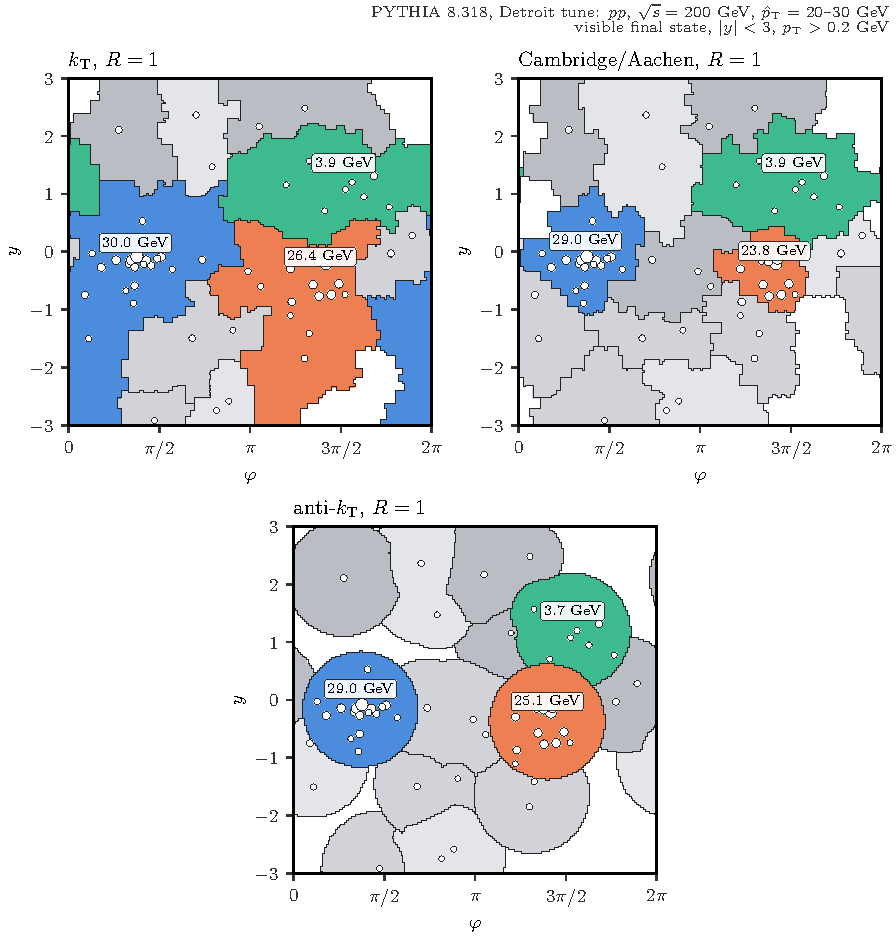
\includegraphics[width=0.7\linewidth]{jet_areas.pdf}
	\caption{Jet areas of one PYTHIA\mbox{-}8 $p+p$ event at $\sqrt{s}=200$~GeV
		(Detroit tune) with the $k_{\rm T}$ (top left), Cambridge/Aachen (top right) and
		anti-$k_{\rm T}$ (bottom) algorithms, $R = 1$. Colored regions are the three
		hardest jets, the same color marking the same jet in every panel; other jets are
		gray. Circles are particles, their area growing with $p_{\rm T}$.}
	\label{fig:jetalgorithms}
\end{figure}
The difference between these algorithms is shown in Fig.~\ref{fig:jetalgorithms} for one simulated event, where each colored region is the area covered by one of the three hardest jets.
%
The \(k_\mathrm{T}\) and Cambridge/Aachen algorithms, which begin by merging soft or nearby particles, produce jets with irregular boundaries that depend on the soft particles of the event, whereas anti-\(k_\mathrm{T}\) clusters around the hardest particles first and gives circular jets of radius \(R\) whose shape is insensitive to soft radiation.  
%
The \emph{FastJet} library~\cite{Cacciari:2011ma} efficiently implements these algorithms and a few more, and is the de-facto standard in the High Energy Physics (HEP) community. 
%
It also provides various recombination schemes. 
\begin{itemize}
	\item \emph{E-scheme}, just adds the four momenta of the jet candidates.  it is the default in FastJet and the most commonly used.
	\item \emph{Boost-invariant $p_t$/$p_t^2$/$E_t$/$E_t^2$ schemes} involve a preprocessing stage rescaling the energy to be equal to the 3-momentum for the
	$p_t$ and $p_t^2$ schemes or the 3-momentum to be equal to
	the energy in the $E_t$ and $E_t^2$ schemes. Then for all schemes the
	recombination $p_r$ of $p_i$ and $p_j$ is a massless 4-vector
	satisfying
	\begin{subequations}
		\begin{align}
			p_{t,r} &= p_{t,i} + p_{t,j}\,,\\
			\phi_r &= \frac{w_i \phi_i + w_j \phi_j}{w_i + w_j}\,,\\
			y_r &= \frac{w_i y_i + w_j y_j}{w_i + w_j}\,,
		\end{align}
	\end{subequations}
	where $w_i$ is $p_{t,i}$ for the $p_t$ and $E_t$ schemes, and is
	$p_{t,i}^2$ for the $p_t^2$ and $E_t^2$ schemes. 
	\item \emph{Winner-takes-all (WTA) scheme} uses the four momentum of the higher momentum jet candidate
\end{itemize}

\section{Heavy-Ion Collisions}
\label{sec:heavyIonCollisions}
\subsection{Quark Gluon Plasma (QGP)}
\label{sec:QGPIntro}
Asymptotic freedom of QCD means that matter at extremely high temperatures and densities (high \(Q^2\)) undergo a \emph{deconfinement} phase transition, with partonic degrees of freedom replacing hadronic degrees of freedom. 
%
This state of deconfined quarks and gluons is called QCD/quark-gluon plasma due to analogous phenomena observed in atomic physics~\cite{SHURYAK198071}.

Thermodynamically, when temperature (\(T\)) or baryon number density (\(n_\mathrm{B}\)) approaches the confinement scale \(\Lambda\) introduced in Sec.~\ref{subsec:runningCoupling} (\(T \sim \Lambda \sim \mathcal{O}(10^{12})K,~\text{and}~n_\mathrm{B} \sim \Lambda^3 \sim 1~\text{fm}^{-3}\)) the boundaries between hadrons become ill defined resulting in hadrons ``melt'' into QGP~\cite{Fukushima_2010}.  
%
For reference, the core of the Sun ``only'' has \(T\sim \mathcal{O}(10^{7})K\) and \(n_\mathrm{B}\sim\mathcal{O}(10^{-14})\text{fm}^{-3}\). 

These orders of \(T\) and \(n_\mathrm{B}\) are the theorized conditions prevalent in the universe a few \(\mu\mathrm{s}\) after Big-Bang. The only natural phenomena in the present-day, cold universe that can achieve these conditions are the cores of neutron stars~\cite{Annala_2020} or neutron star mergers~\cite{neutronStarMerger}. Artificially, the required  \(T\) and \(n_\mathrm{B}\) can be achieved at facilities like the Large Hadron Collider (LHC) and Relativistic Heavy Ion Collider (RHIC) through collisions of heavy-ions (like Au, Pb, etc.) at near-light speeds, the aptly named \emph{little bangs}. The rest of this section describes these collisions and the evolution of the matter they produce.

\subsection{Space-time evolution of a heavy-ion collision}
\label{sec:qgpSpacetime}

\begin{figure}
	\centering
	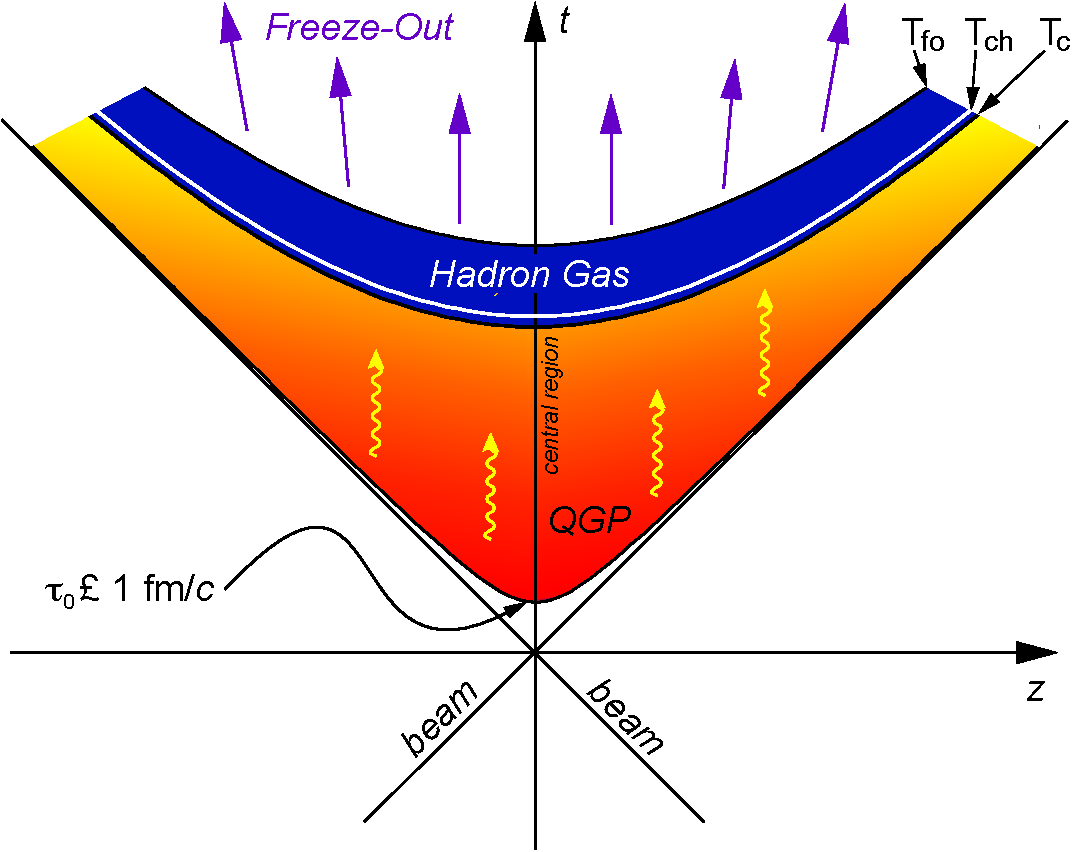
\includegraphics[width=0.7\linewidth]{figures/LightCone1_color-crop}
	\caption{A light cone diagram showing the stages of a heavy ion collision.  The abbreviation  $T_{\mathrm fo}$ is for the thermal freeze-out temperature, $T_{\mathrm ch}$ is for the chemical freeze-out temperature, and $T_{\mathrm c}$ is for the critical temperature where the phase transition between a hadron gas and a QGP occurs.  $\tau_0$ is the formation time of the QGP. Taken from~\cite{Connors_2018}.}
	\label{fig:lightcone}
\end{figure}

Estimates of the energy density indicate that heavy ion collisions at RHIC and LHC  reach energy densities ranging between 1-12 GeV/fm$^3$~\cite{PhysRevC.93.024901,PhysRevC.94.034903}, well in excess of the 0.2-1 GeV/fm\(^3\) required for QGP formation~\cite{PhysRevD.90.094503,Karsch2002}. 
%

%\subsection{Space-time picture of QGP}
The heavy ion collision and the evolution of the fireball, as depicted in Fig.~\ref{fig:lightcone}, has several stages, and the measurement of the final state particles can be affected by one or all of these stages depending on their production mechanism and interaction time within the medium. 
%
Immediately after the collision, the system is in a non-thermalized, pre-equilibrium state where, partons undergo hard scattering, dominated by \(2\to 2\) QCD processes with the outgoing partons back-to-back in azimuth (\(\Delta \phi \approx \pi\)). 
%
At \(\tau \approx 0.5 - 1~\text{fm}/c\), the system thermalizes into the QGP state which expands following hydrodynamic laws. 
%
During the expansion, the system cools down until it reaches the temperature (\(T_c \approx 156\)~MeV from lattice QCD studies) at which a crossover phase transition to a hadronic gas state occurs. 
%
By \(\tau \approx 10~\text{fm}/c\) after the collision, confinement is restored and colored partons hadronize into colorless hadrons.
%
At chemical freeze-out, which occurs close to \(T_c\) (statistical-model fits give \(T_{ch} \approx 155\text{--}165\)~MeV), the particle abundances of the system are frozen. 
%
Elastic interactions can still occur till the kinetic freeze-out (\(T_{fo} \approx 100\)~MeV), where the particle momentum spectra are established.


%\begin{figure}[h]
%	\centering
%	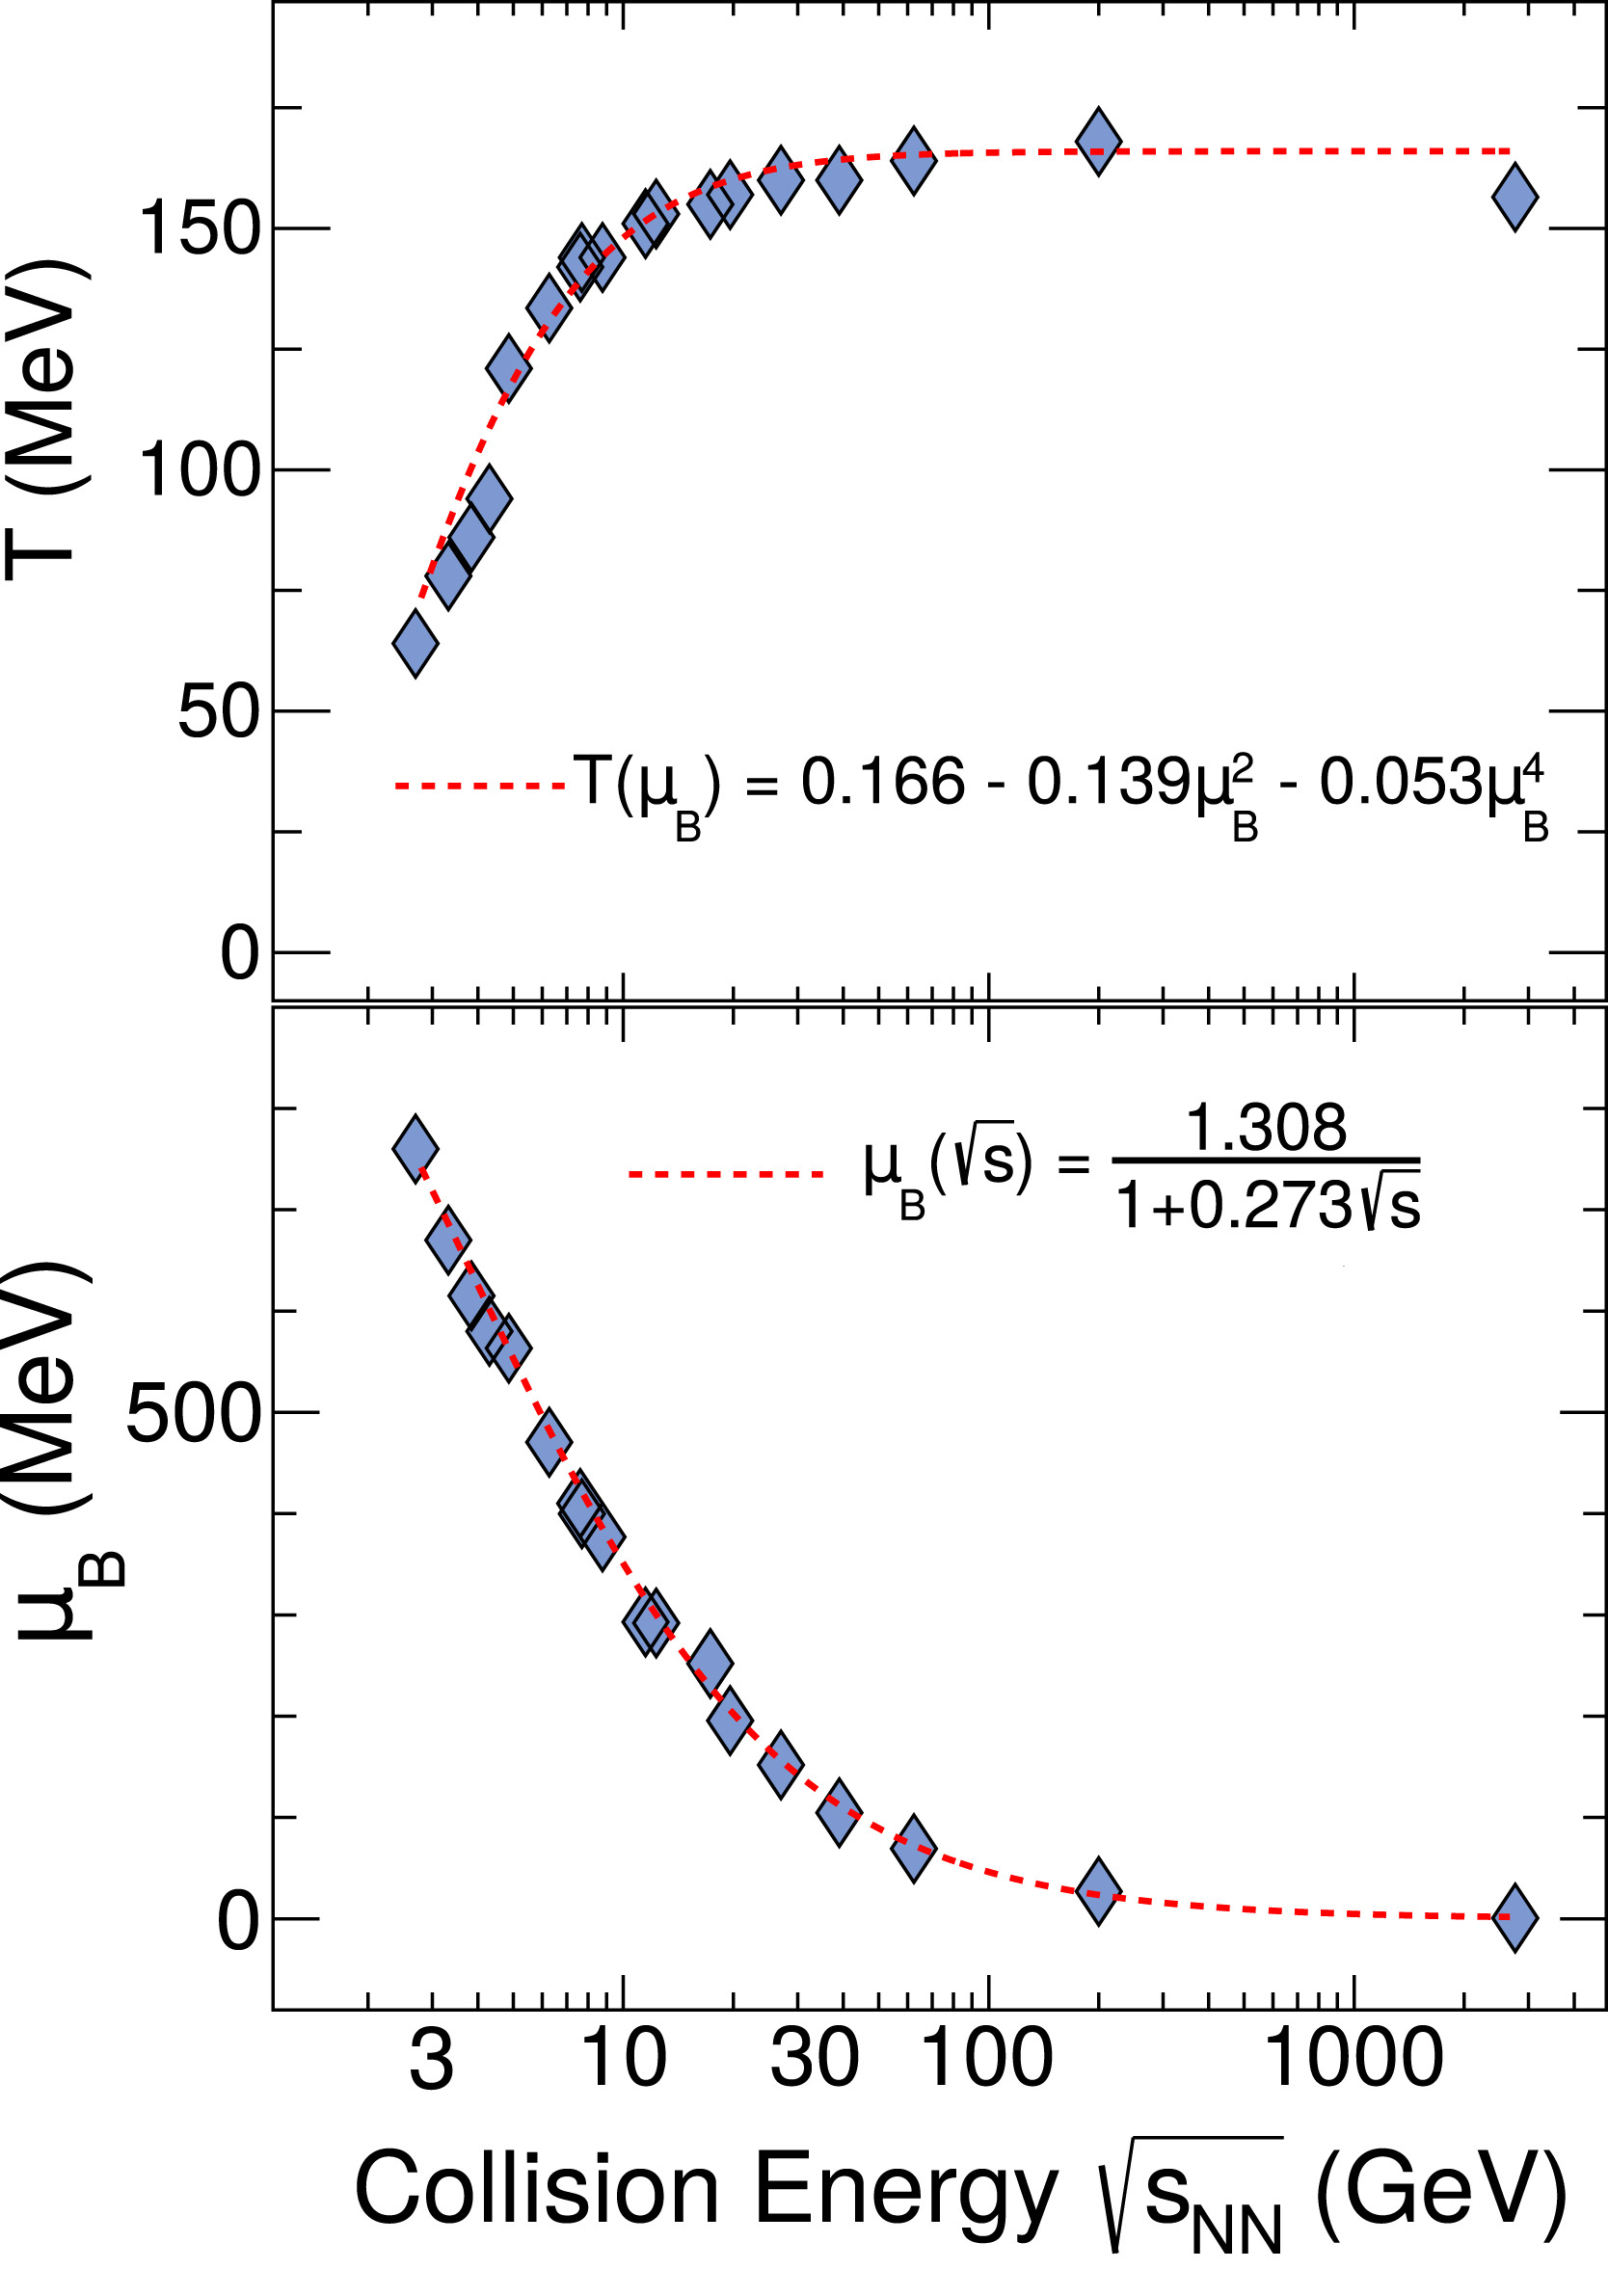
\includegraphics[width=0.5\linewidth]{figures/T_mu_vs_sNN}
%	\caption{Chemical freeze-out parameters \(T\) and \(\mu_\mathrm{B}\) obtained by thermal model fits to experimental data on particle yields as a function of collision energies. Red line represents parametrizations of \(T\) and \(\mu_\mathrm{B}\) as a function of $\sqrt{s_\mathrm{NN}}$}
%	\label{fig:tmuvssnn}
%\end{figure}
\subsection{Initial State of Colliding Nuclei}
Nuclei like $\rm ^{197}_{79}Au$, $\rm ^{96}_{40}Zr$, $\rm ^{96}_{44}Ru$,  etc. are complex arrangements of protons and neutrons that have a multitude of non-trivial initial configurations leading up to their collisions, which have significant effects on the final state particle distributions.
%
Therefore, any measurement done using heavy-ion events needs to report these initial configurations of the colliding nuclei.
%
The initial state of the incoming nuclei is not precisely known, but its properties impact the production of final state particles.  
%
The incoming nuclei are often modeled as either an independent collection of nucleons called a Glauber initial state~\cite{Miller:2007ri}, or a wall of coherent gluons called a Color Glass Condensate~\cite{IANCU2001583}. 
%
The widely used model for determining these quantities is the Glauber Monte Carlo (Glauber MC) model~\cite{Loizides_2015}, which assumes Woods--Saxon density distribution of nucleons.
%
The nuclei are then assigned a random impact parameter and translated to collide. 
%
If the distance between centers of nucleons is less than \(\sqrt{\sigma_\mathrm{inel}^\mathrm{NN}/\pi}\), where \(\sigma_\mathrm{inel}^\mathrm{NN}\) is the inelastic nucleon–nucleon cross section, the nucleons have undergone a binary collision. 
%
Nucleons that have undergone at least one binary collision are said to have participated in the reaction.
%
This procedure is followed to obtain the number of participant nucleons (\(N_\mathrm{part}\)) and the number of binary collisions (\(N_\mathrm{coll}\)) event-by-event.

A schematic diagram of the geometry of heavy-ion collisions is shown in Fig.~\ref{fig:hictikz}. 
\begin{figure}
	\centering
	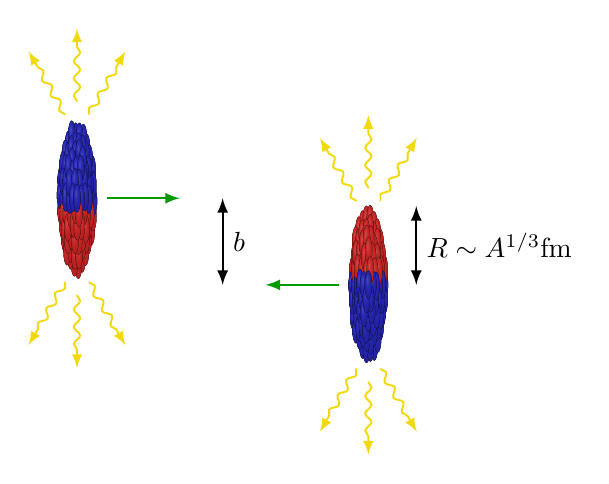
\begin{tikzpicture}
		\def\N{85} % number of nucleons
		\def\R{1.0} % nucleus radius
		\def\Nlay{5} % number of rings/layers
		\def\xs{0.25} % horizontally scale
		\def\Rp{0.92} % length photon
		\def\D{3.7} % horizontal distance between nuclei
		\pgfmathsetmacro\H{1.10*\R} % vertical distance between nuclei
		\pgfmathsetmacro\v{0.25*\D} % length vector
		
		%\message{^^J PbPb collision with impact parameter}
		
		% NUCLEUS
		% participants: nucleons in the vertical band where the two nuclei overlap
		\pic[xscale=\xs,nucleus participants,nucleus ymin=-\R,nucleus ymax=\R-\H] (L) at (-\D/2, \H/2) {nucleus};
		\pic[xscale=\xs,nucleus participants,nucleus ymin=\H-\R,nucleus ymax=\R] (R) at ( \D/2,-\H/2) {nucleus};
		
		% VELOCITY VECTORS
		\draw[vector] (L-0)++(2pt,0) --++ (\v,0); %node[above=2pt] {$v\approx c$};
		\draw[vector] (R-180)++(-2pt,0) --++ (-\v,0); %node[above=2pt] {$v\approx c$};
		
		% PHOTONS
		\foreach \ang in {60,90,120,-60,-90,-120}{
			\draw[photon] (L-\ang) --++ (\ang:\Rp);
			\draw[photon] (R-\ang) --++ (\ang:\Rp);
		}
		
		% MEASURES
		\draw[<->,thick]
		(R-0)++(0.3*\R,0) --++ (0,\R) node[midway,right] {$R\sim A^{1/3}\mathrm{fm}$};
		\draw[<->,thick]
		(0,-\H/2) -- (0,\H/2) node[midway,right] {$b$};
		%\node at (0.3*\D,0.7*\H) {$b > 2R$};
		
	\end{tikzpicture}
	\caption{Typical heavy-ion collision with an impact parameter of \(b\). The participating nuclei are colored red and the spectators are colored blue.}
	\label{fig:hictikz}
\end{figure}

\subsection{Centrality Determination} \label{sect:CentEP}
\begin{figure}[h]
	\centering
	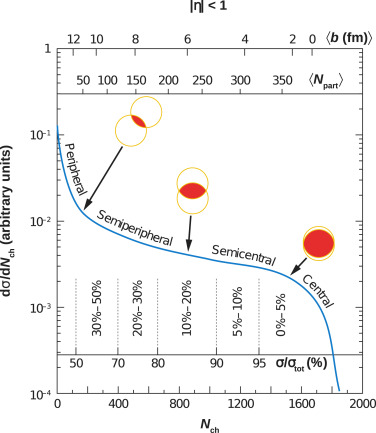
\includegraphics[width=0.6\textwidth]{figures/centrality_refmult.jpg}
	\caption{An illustration of the total inclusive charged particles multiplicity \(N_\mathrm{ch}\) and number of participant (\(N_\mathrm{part}\)) and impact parameter (\(b\)) in heavy-ion collisions. Taken from~\cite{Miller:2007ri}.}
	\label{fig:centralityVsNch}
\end{figure}
As the impact parameter  (\(b\)) of collisions, the distance between the geometrical centers of the colliding nuclei, is not measurable in experiments, a proxy called \emph{centrality} is defined. 
%
Centrality is characterized by the charged particle multiplicity of events, connected to the impact parameter through a simulation defining it as a function of \(N_\mathrm{part}\), \(N_\mathrm{coll}\) 
and impact parameter \(b\) from Glauber model is mapped with the experimental data through a particle production model called the Two-Component Model~\cite{KHARZEEV2001121}. 
%
Assuming that particle production is governed by contribution from hard component (\(\propto N_\mathrm{coll}\)) and soft component (proportional to  \(\propto N_\mathrm{part}\)), it simulates the multiplicity distribution according to
\begin{equation}
	\frac{dN_\mathrm{ch}}{d\eta} = n_{pp}\left[xN_\mathrm{coll} + (1-x)\frac{N_\mathrm{part}}{2}\right]
\end{equation}
where the quantity \(n_{pp}\) is the multiplicity from a \(p+p\) collision of the same center-of-mass energy. \(x\) is the contribution of hard component. 
%
\(n_{pp}\) is drawn from a negative binomial distribution with parameters \(\text{NBD }(n_{pp}; \langle n_{pp}\rangle,k)\), where \( \langle n_{pp}\rangle\) is the average multiplicity in the \(p+p\) collision and \(k\) is the width of the distribution. 
%
The simulated charged multiplicity distribution is then fitted with the corresponding multiplicity distribution from the experiment. \(\langle n_{pp}\rangle\), \(k\), and \(x\) are kept as free parameters in the fitting to experimentally measured charged particle multiplicity distribution. 																		
%
Initial guess values for \(x\) could be set close to those determined in different experiments for faster convergence of fitting~\cite{back2004collision,PhysRevC.88.044909}. 

An event belongs to a centrality class, say 0\%–5\% if its charged particle multiplicity falls in the top \(5^\text{th}\) percentile. 
%
Fig.~\ref{fig:centralityVsNch} illustrates collision centrality definition in heavy-ion collisions by comparing the charged particle multiplicities with Glauber MC + Two-component model simulation.
%
Centrality classes are classified for the simulated distribution. 
%
\(\langle N_\mathrm{part}\rangle\), \(\langle N_\mathrm{coll}\rangle\) in those centrality classes are calculated. 

\subsection{Anisotropic flow}
\label{sec:flowIntro}
\begin{figure}[h]
	\centering
	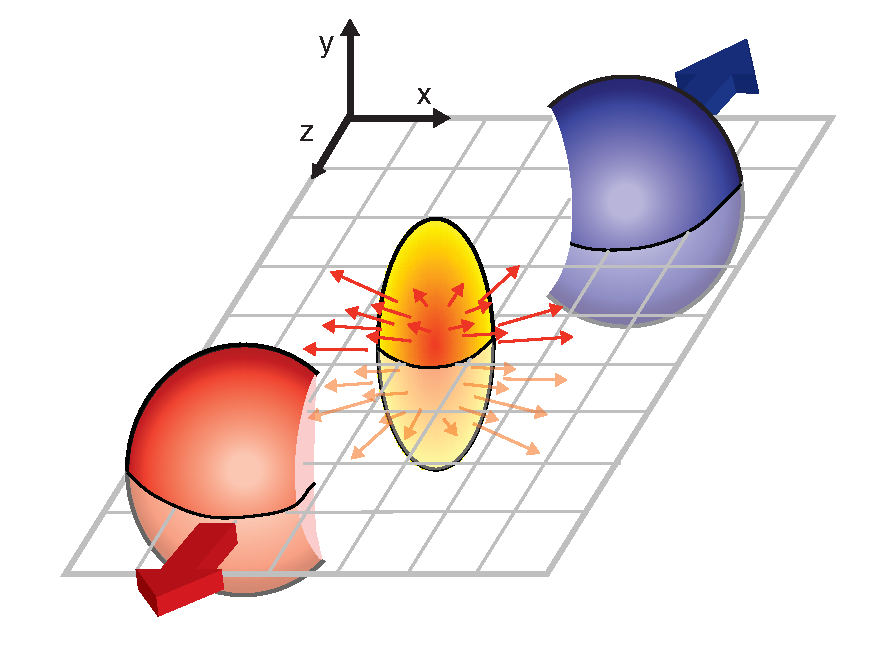
\includegraphics[width=0.4\textwidth]{figures/flow_elliptic_init_v4.pdf}
	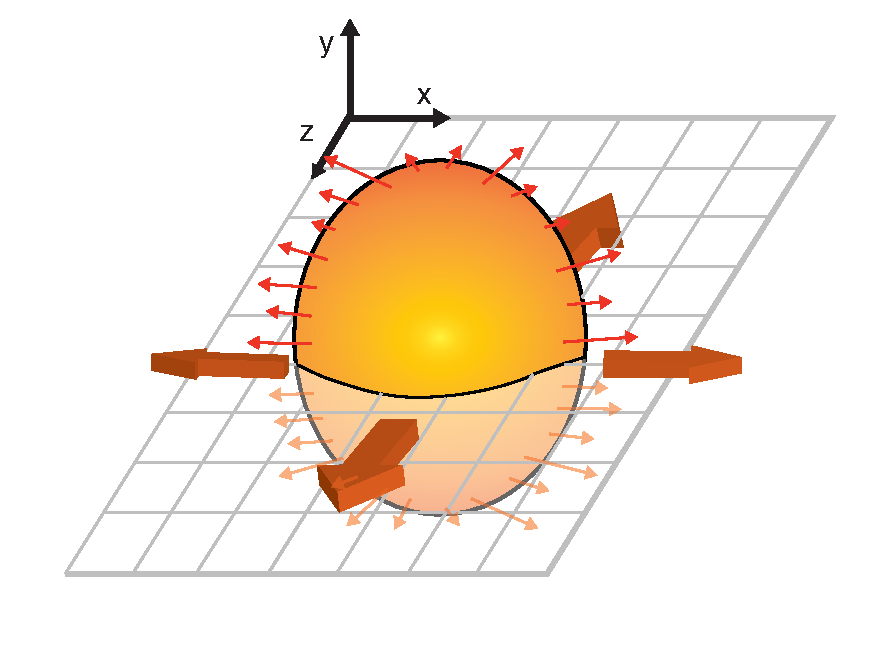
\includegraphics[width=0.4\textwidth]{figures/flow_elliptic_expd_xyz_v2.pdf}
	\caption{Schematic diagrams of a non-central heavy-ion collision: the almond-shaped overlap region of the two nuclei with its anisotropic pressure gradients (left), and the resulting momentum anisotropy of the expanding medium, with more particles emitted along the short axis of the overlap region (right). This anisotropy is quantified by the Fourier coefficients \(v_n\) of the azimuthal particle distribution. Taken from~\cite{Connors_2018}.}
	\label{fig:anisotropycartoon}
\end{figure}
Contrary to initial naive expectations of a gas-like QGP, the QGP formed in these collisions was shown to behave like a liquid of quarks and gluons~\cite{Heinz_2013}.
%
Thus, mean free path of particles in QGP fireball is much smaller than the fireball's system size.
%
Hence, in non-central heavy ion collisions the initial state coordinate space asymmetry generates a pressure gradient in the direction of the impact parameter $b$, schematically shown in Fig.~\ref{fig:anisotropycartoon} (left). 
%
This spatial asymmetry translates into an azimuthal momentum anisotropy as the system expands (Fig.~\ref{fig:anisotropycartoon}, right), meaning that particles are more likely to be emitted along the plane where the pressure gradients are the highest. 
%
This plane is defined by the beam axis and the impact parameter of the collision, and called the \emph{reaction plane} (\(\Psi_{\rm RP}\)).
%
The anisotropy can be characterized by the Fourier decomposition of the azimuthal particle distribution with respect to \(\Psi_{\rm RP}\)~\cite{Bielcikova:2003ku,Voloshin:1994mz}:
\begin{equation}
	\frac{dN}{d(\phi - \Psi_{RP})} = \frac{N_0}{2\pi} \left( 1 + 2 \sum_{n=1}^{\infty} v_n \cos[n(\phi - \Psi_{RP})] \right),
	\label{fourier_azi_part_distr}
\end{equation}
%
The \emph{anisotropic flow} coefficients $v_{n}$, the $n^{\rm th}$ order term in the Fourier decomposition of the final state particle azimuthal distribution is given by,
%
\begin{equation}
	\label{flow}
	v_{n} = \left< \cos([n(\phi - \Psi_{\rm RP})]) \right>
\end{equation}
%
Due to the symmetry of the collision geometry, the most prominent contribution is from the second order coefficient $v_2$, called \emph{elliptic flow}.

\begin{figure}[h]
	\centering
	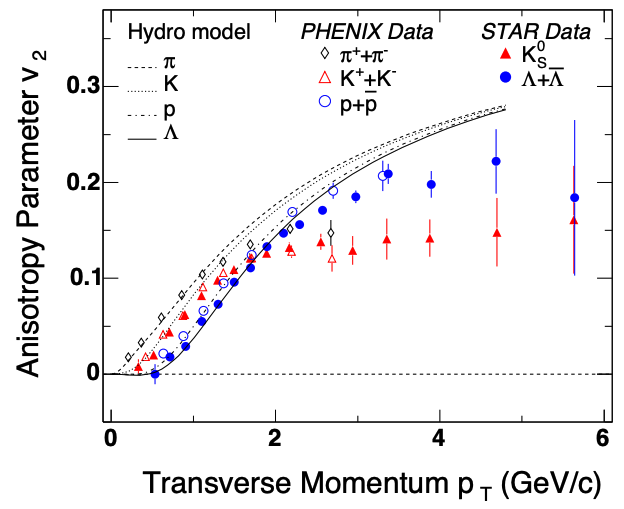
\includegraphics[width=0.41\linewidth]{AnisotropyWithNoScaling (1).png}
	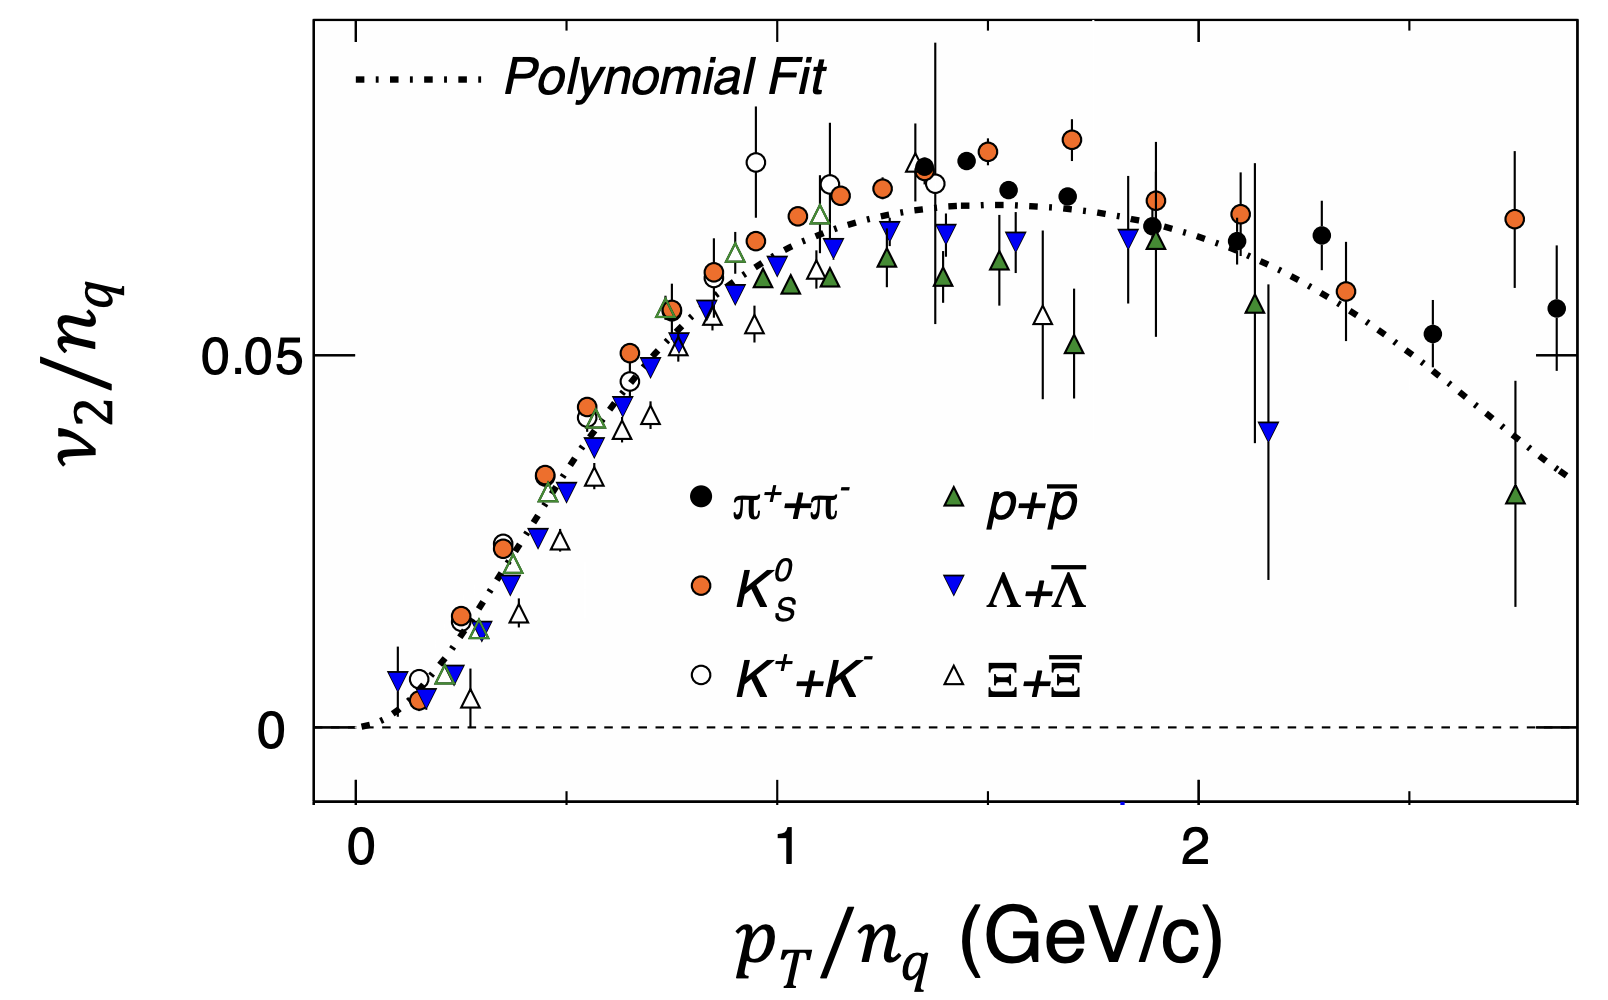
\includegraphics[width=0.52\linewidth]{Gen1_IdentifiedParticle_v2.png}
	\caption{\textbf{Left panel}: Elliptic flow $v_2$ for several particle species in Au+Au collisions at \sNN{200}{GeV}  from STAR and PHENIX experiments. Predictions from hydrodynamic models are shown as lines. Taken from \cite{GYULASSY200530}. \textbf{Right panel}: Number of constituent quarks ($n_q$) scaled $v_2$ as a function of $p_{\rm T}/n_q$. Taken from \cite{Sorensen_2006}.}
	\label{fig:AnisotropyResults}
\end{figure}

$v_2$ was measured by the STAR and PHENIX for several particle species and is shown in Fig.~\ref{fig:AnisotropyResults}.
%
Below \(p_\mathrm{T} \approx 2\)~GeV/\(c\) (left panel), \(v_2\) rises with \(p_\mathrm{T}\) and is ordered by hadron mass, lighter hadrons having larger \(v_2\), as predicted by the hydrodynamic calculations, while at higher \(p_\mathrm{T}\) it saturates below the hydrodynamic curves, with baryons above mesons. 
%
Large positive $v_2$ values indicate collective phenomena associated with a strongly coupled fluid, or a \emph{signature of QGP}.
%
A scaling of the $v_2$ values with the number of constituent quarks (2 for mesons, 3 for baryons) yielded a universal curve as a function of $p_{\rm T}/n_q$ (right panel) suggesting the flow dynamics were developed in a medium with quark and gluon degrees of freedom, i.e. QGP.


\section{Jets in QGP}
\label{sec:jetsInQGP}
As discussed in Sec.~\ref{sec:qgpSpacetime}, hard scatterings of partons that produce jets happens before the system thermalizes into QGP (parton producing a 10~GeV jet scatters at \(\tau \sim 1/E \sim 0.2\text{fm}/c\)). 
%
Thus the ensuing parton shower traverses the QGP, and resulting jet is \emph{modified/quenched} compared to an appropriate \emph{baseline}. 
%
The two main mechanisms for jet quenching are \emph{collisional} and \emph{radiative} energy losses. 
%
Collisional energy loss happens due to the elastic scattering between the parton and the medium constituents and usually dominates for lower energy partons. 
%
Radiative energy loss happens due to induced gluon radiation (\textit{bremsstrahlung}) through inelastic scatterings with the medium particles \cite{MAJUMDER201141,QinWang2024,Burkeetal}. 
%
For partons with \ptGeq{parton}{5} , this is usually the dominant source of energy loss \cite{LandoltBornstein2010:sm_lbs_978-3-642-01539-7_16}. 
%
%\subsection{Combinatorial background in heavy-ion jets}
%Final state of heavy-ion collisions is characterized by a massive \emph{Underlying Event}, arising from the thermalized QGP. 
%%
%Although useful for bulk calculations like elliptic flow, including them in the jet clustering would artificially inflate the amount of radiation in the jet cone, as we generally want to restrict the jet constituents to remnants of a parton shower. 
%%
%This background is generally uncorrelated to the jet and hence called \emph{Uncorrelated/Combinatorial Background}.  
%%
%Heavy-ion jet background subtraction is quite an active field of study. 
%%
%The method of background subtraction is different for different jet analysis. 
%
%For 

%\subsection{Heavy-ion jet measurements}
The baseline measurement is done in a collision system where either QGP is not formed or has negligible lifetime compared to central heavy-ion collisions. 
%
Two possible choices arise for the baseline, first is \(p+p\) collisions, from which one can calculate the \emph{Nuclear Modification Factor} (\RAA) for distributions of any observable \(\mathbf{O}\) calculated in \(p+p\) and \(A+A\) collisions,
given by
\begin{equation}
	R_{\rm AA}(\mathbf{O}, b) = \frac{dN_{\rm AA}/d\mathbf{O}}{\left<T_{\rm AA}(b)\right> . d^2\sigma_{pp}/d\mathbf{O}}
\end{equation}\label{RAA}
where $T_{\rm AA}(b) = N_{\rm coll}(b)/\sigma_{\rm NN}^{\rm inel}$ is the nuclear overlap function  which determines the number of participating nucleons and number of binary collisions $N_{\rm bin}$ for a heavy ion collision as a function of its impact parameter (\textit{b})~\cite{doi:10.1142/S0217751X95001467}.
%
The second common baseline used in absence of a \(p+p\) baseline is peripheral collisions of heavy-ion collisions. The \emph{Relative Nuclear Modification Factor} \(R_{CP}\) is given by,
%
\begin{equation}
	R_{CP}(\mathbf{O}, b) = \frac{dN/d\mathbf{O}}{\left< N_{\rm bin}(b) \right>} \biggm\lvert_{\rm cent} \times \frac{\left< N_{\rm bin}(b) \right>}{dN/d\mathbf{O}} \biggm\lvert_{\rm peri}
	\label{eq:IntroRCP}
\end{equation}

\begin{figure}
	\centering
	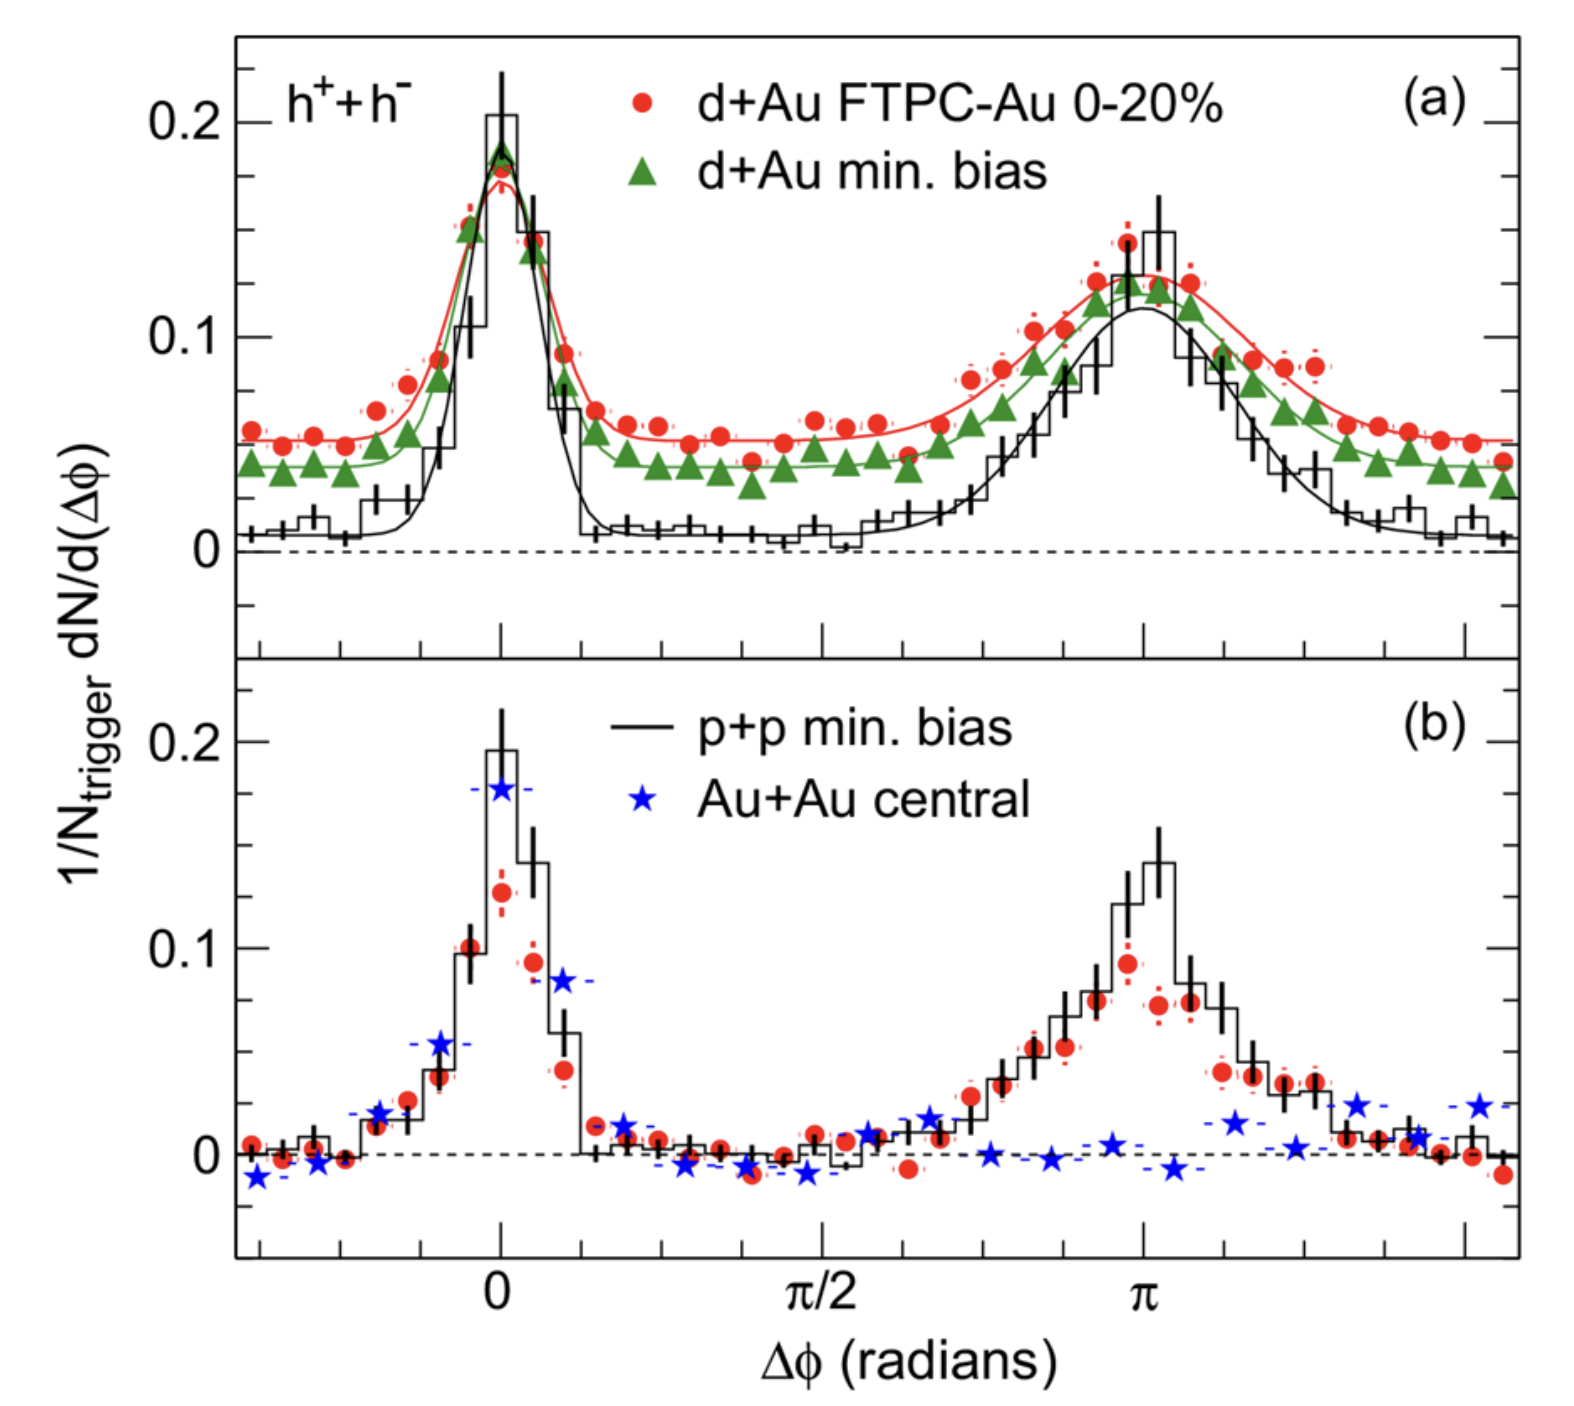
\includegraphics[width=0.8\linewidth]{Gen0_AngularCorrelation_JetQuenching.png}
	\caption{Measurement of the angular correlation between all charged hadrons and the leading hadron in the event for p+p (black lines), d+Au (red and green markers), and Au+Au events (blue markers), performed by the STAR experiment. The vanishing of the away-side yield around $\Delta\phi\approx \pi$ in Au+Au events is evidence of particles getting quenched in the QGP medium. Taken from \cite{Adams:2003im}.}
	\label{fig:angularcorr}
\end{figure}

Before infrastructure became available to reliably reconstruct a sufficient number of jets in heavy-ion collisions,  the effects of the medium on high energy partons were studied through the \emph{Di-hadron correlation}. 
%
Leading hadron (highest $p_\mathrm{T}$ in event) is used as a jet proxy and the azimuthal angular correlation ($\Delta\phi$) of all charged hadrons in the event is studied.
%
Fig.~\ref{fig:angularcorr} shows one of the first measurements performed by STAR~\cite{Adams:2003im}, di-hadron correlations compared between p+p, Au+Au, and d+Au collisions. 
%
The p + p and d+Au both show peaks around $\Delta\phi = 0$ and $\Delta\phi =  \pi$ as expected, given that hard scatterings are dominated by \(2\to 2\) Feynman diagrams. 
%
However, for Au+Au collisions, the peak around $\Delta\phi = \pi$ completely vanishes. 
%
This was the expectation because depending on the distance from the center of the collision where the initial back-to-back partons were produced, one of the partons would travel a larger distance in the QGP medium and therefore lose more energy than the other one.

\begin{figure}
	\centering
	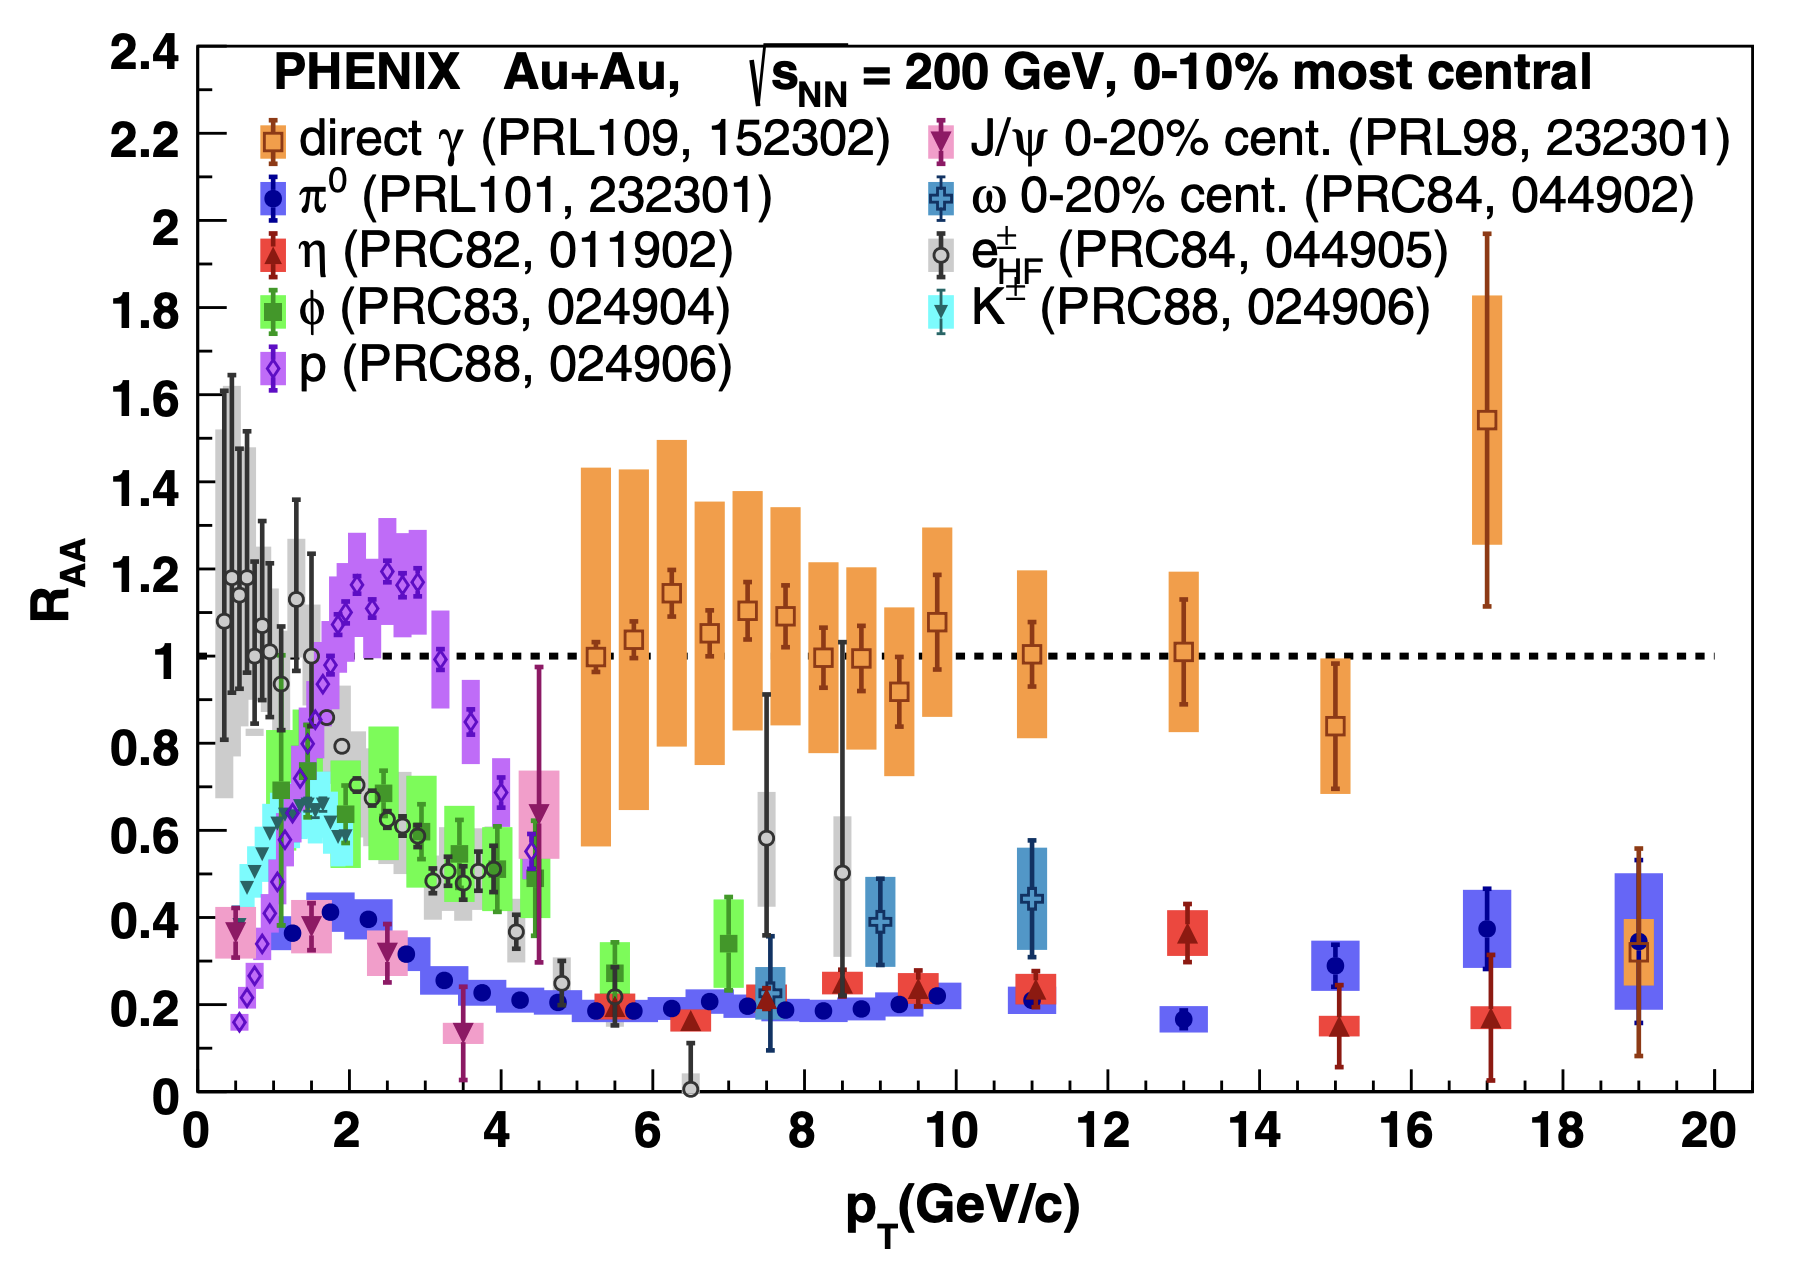
\includegraphics[width=0.8\linewidth]{Gen0_SingleParticle_RAA.png}
	\caption{Nuclear modification factor $R_{\rm AA}$ as a function of $p_\mathrm{T}$ for identified particle species in Au+Au collisions at \sNN{200}{GeV} measured by the PHENIX experiment. Taken from \cite{Tannenbaum_2015}.}
	\label{fig:singleparticleraa}
\end{figure}

A closer look at jet quenching was given by the PHENIX experiment through a collection of  \RAA~measurements discussed in Eq.~\ref{RAA} for identified particles spectra, shown in Fig.~\ref{fig:singleparticleraa}.
%
Whereas, direct photons ($\gamma$) do not interact strongly, and hence have no yield modification in the medium.
% 
All strongly interacting particles show varying levels of suppression from 0.2 - 0.6, again confirming their energy loss in the presence of QGP.

Although measurements with high $p_\mathrm{T}$ hadrons help to understand jet quenching mechanisms in the medium, they suffer from survival bias, as these hadrons arise from a subsample of jets which usually undergo the least amount of quenching \cite{PhysRevC.99.051901}. 
%
Fully reconstructed jets, however, are mostly unbiased probes of energy flow at high $p_\mathrm{T}$, and offer a wealth of substructure observables which give access to the energy flow within the jet more differentially.
%


\begin{figure}
	\centering
	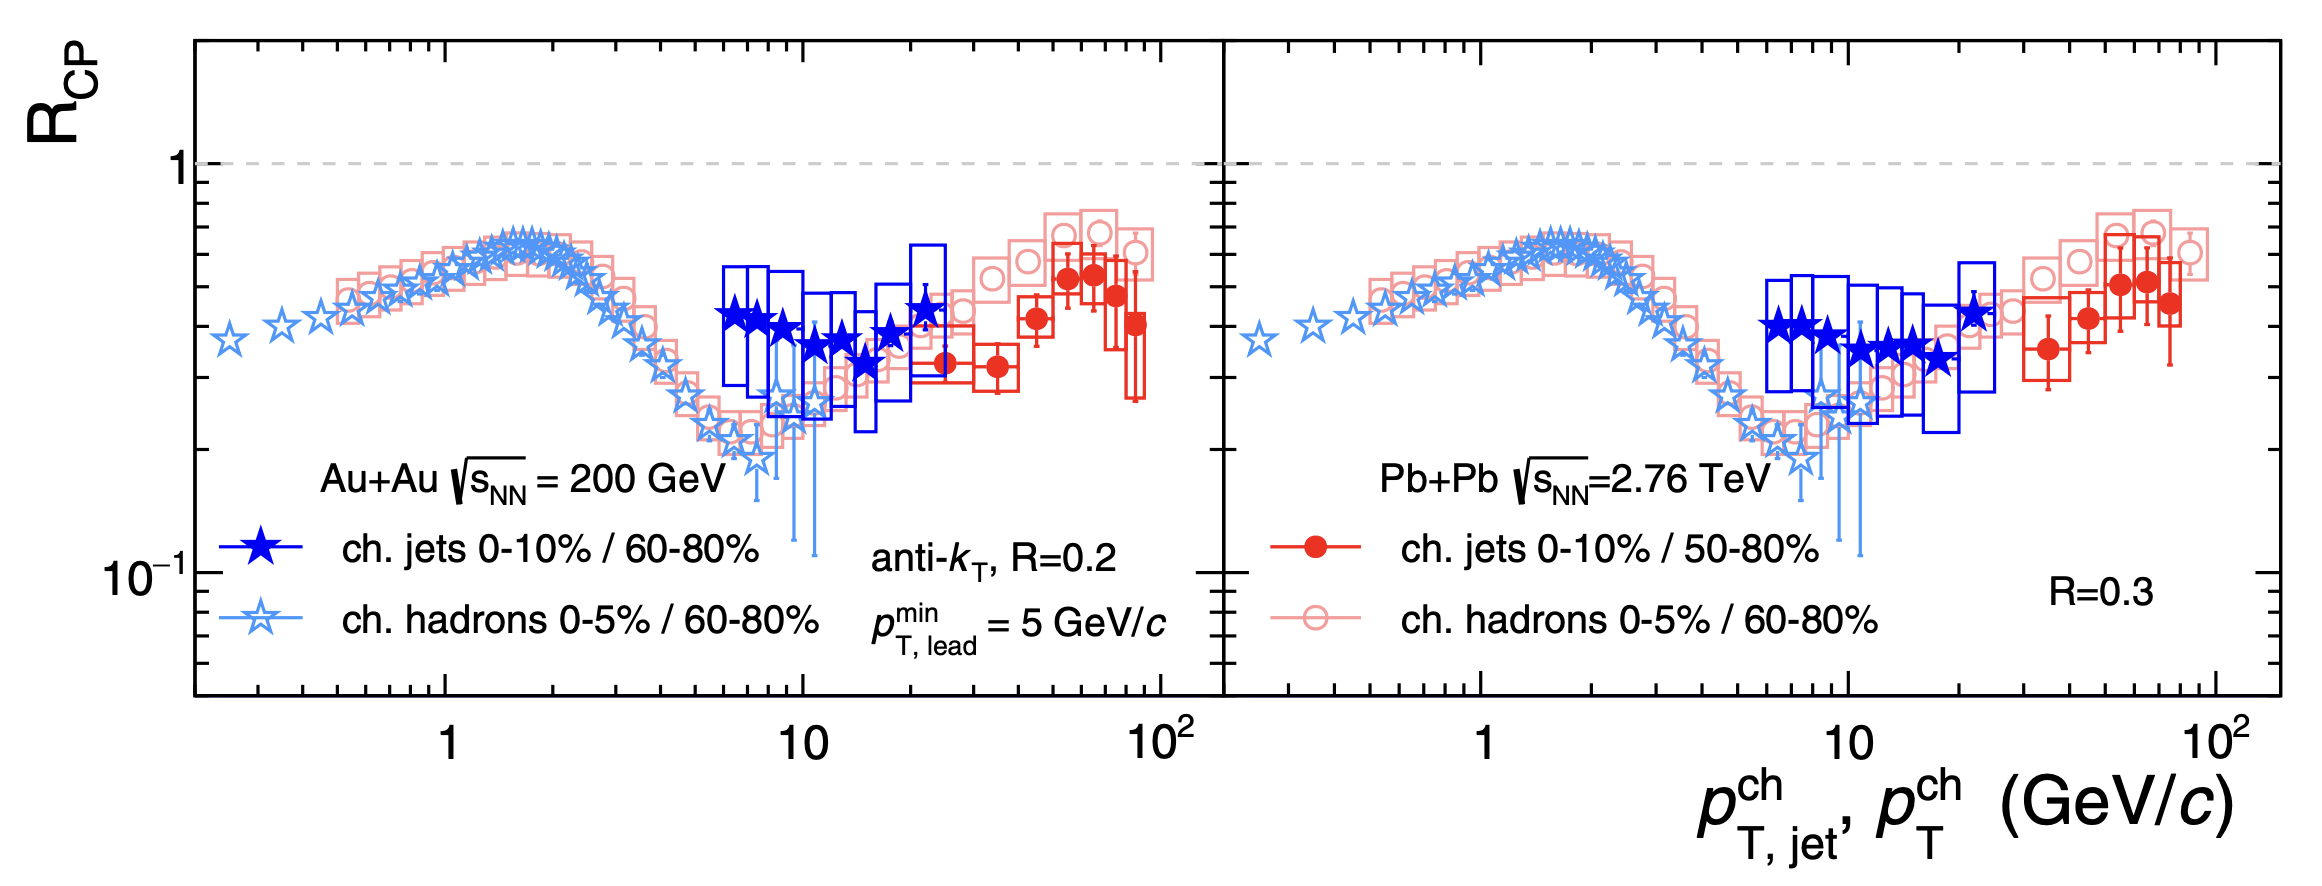
\includegraphics[width=1\linewidth]{Gen1_ChargedParticleAndJets_RCP.png}
	\caption{$R_{CP}$ distributions for charged hadrons (open markers) and jets (solid markers) from RHIC (blue star markers) and LHC (red circle markers) experiments. Taken from \cite{STARChargedJet} and references within \cite{PhysRevLett.91.172302,ALICEChargedJet,ATLASChargedHadron}.}
	\label{fig:chargedparticlercp}
\end{figure}
The STAR experiment measured the \(R_{CP}\) of the $p_\mathrm{T}$ spectra of charged particle jets (clustered charged tracks only and contain no calorimeter hits (towers) as input) from central and peripheral Au+Au collisions at \sNN{200}{GeV} shown in Fig.~\ref{fig:chargedparticlercp} \cite{STARChargedJet}. 
%
Measured for charged jets was compared to $R_{CP}$ for charged hadrons from STAR at the same energy, and to the measured $R_{CP}$ for charged hadrons and jets from the ALICE and ATLAS experiments at \sNN{2.76}{TeV}. 
%
First, the charged hadrons $R_{CP}$ is found to be the same over the same range of $p_\mathrm{T}$ at RHIC and LHC energies (which are an order of magnitude apart). 
%
The charged jet $R_{CP}$ is also found to have similar values between RHIC and LHC energies with the charged-jet yield in central collisions suppressed by roughly 60\% relative to scaled peripheral collisions, with no significant $p_\mathrm{T}$ dependence in contrast to the $p_\mathrm{T}$ dependence observed for the charged hadrons $R_{CP}$. 
%
This may be because the inclusive hadron distribution usually arises from the leading hadron in the corresponding jet, and is therefore is sensitive to the fragmentation function. 
%
This fragmentation process can therefore introduce the $p_\mathrm{T}$ dependence of $R_{CP}$ in hadrons. 

\begin{figure}
	\centering
	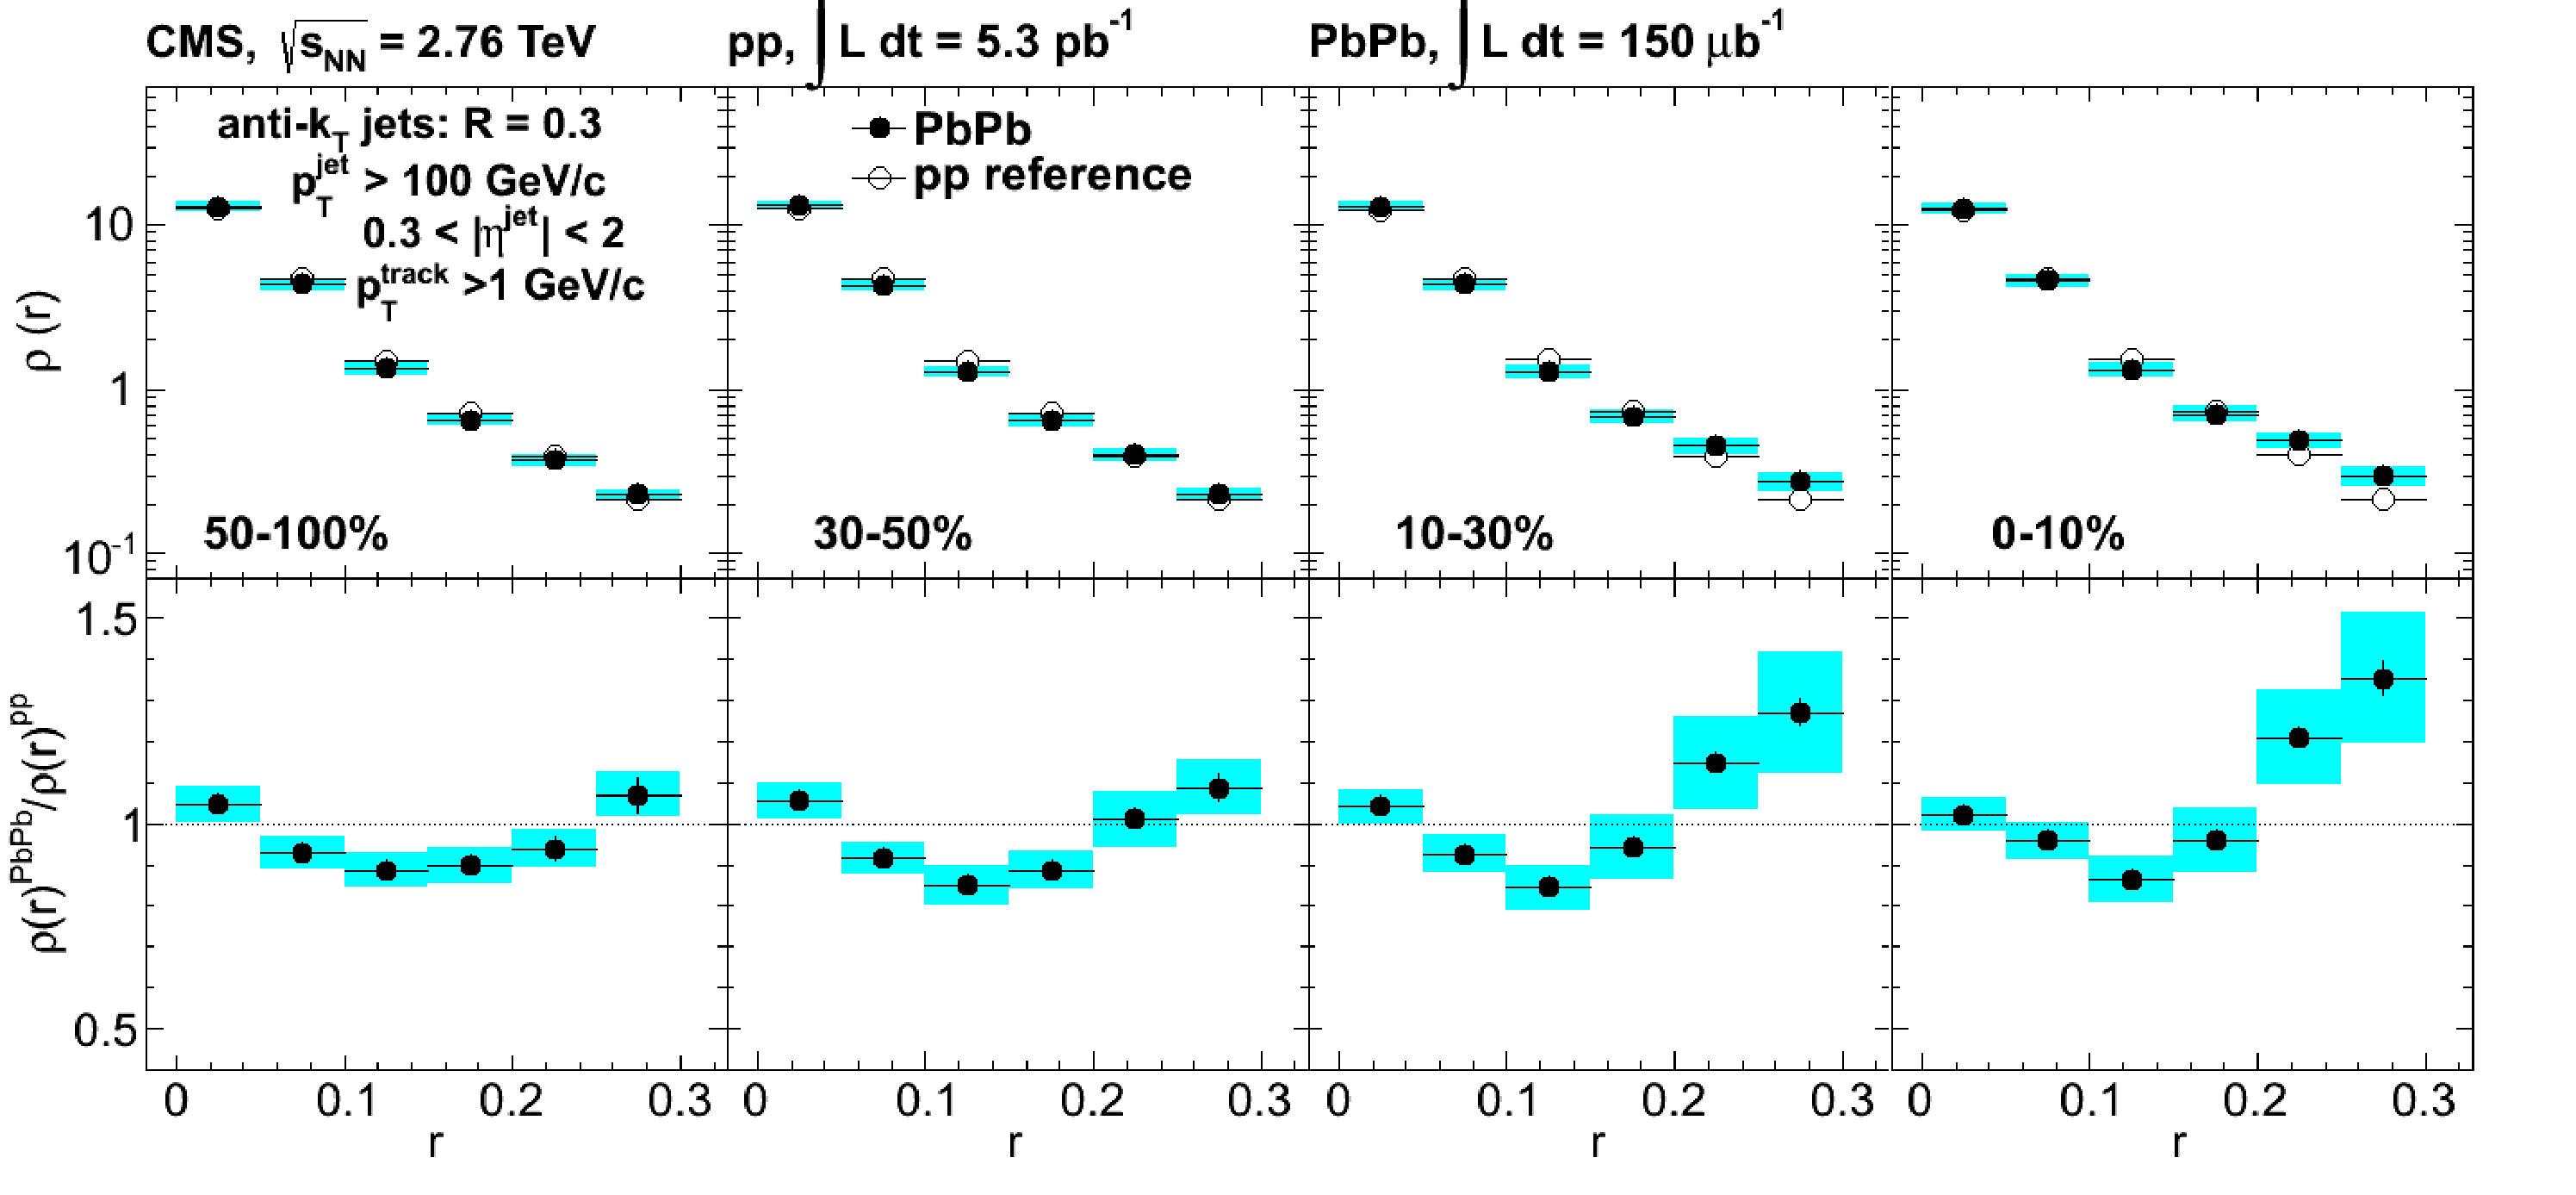
\includegraphics[width=\linewidth]{figures/CMSJetShapeFinalJS4Cent}
	\caption{Differential jet shapes in Pb+Pb and \(p+p\) collisions for four Pb+Pb  centralities. Each spectrum is normalized so that its integral is unity.  In central collisions a larger fraction of the jet momentum is found at large angles relative to the jet axis, as expected from partonic energy loss. Taken from~\cite{Connors_2018}.}
	\label{fig:cmsjetshapefinaljs4cent}
\end{figure}
Going a bit into the jet substructure, CMS measurement of jet's average radial momentum profile around the jet-axis, called \emph{differential jet shape} defined as,
\begin{equation}
	\rho(r) = \frac{1}{\delta r} \frac{1}{N_{\mathrm jet}} \sum_{\mathrm jets} \frac{ \sum_{{\mathrm tracks} \epsilon [r_a, r_b)} p_{T}^{\mathrm track}}{p_{T}^{\mathrm jet}}
	\label{eq:rhoVsDr}
\end{equation}
%
where the jet cone is divided rings of width $\delta r$ which have an inner radius $r_a$ and an outer radius $r_b$.  
%
From the results shown in Fig.~\ref{fig:cmsjetshapefinaljs4cent}, the differential jet shapes in the most central Pb+Pb collisions are broadened in comparison to measurements done in \pp collisions at the same center of mass energy ~\cite{Chatrchyan:1605718}.  
%
These measurements demonstrate that there is an enhancement in the modification with increasing angle from the jet axis, indicating a broadening of the jet profile and a depletion near r~$\approx$~0.2.
%
These measurements motivate the studies presented in Chs.~\ref{ch:jhcorr} and~\ref{ch:angularities}: the dependence of jet quenching on the path length through the medium, and the angular structure of jets in vacuum and in the QGP.

\section{Outline}
This thesis uses jets to study QCD in vacuum and in the QGP with two measurements at \sNN{200}{GeV}: the dependence of jet quenching on the path length through the medium, and the angular structure of jets, which records the history of their showers.
%
Ch.~\ref{ch:STAR} describes RHIC and the STAR detector.
%
Ch.~\ref{ch:jhcorr} presents jet-hadron correlations relative to the event plane in \AuAu collisions.
%
Ch.~\ref{ch:angularities} presents generalized angularities of jets, first in \AuAu collisions and then, inclusive and groomed, in \pp collisions.
%
Ch.~\ref{ch:summary} summarizes the results and gives an outlook.
%
The appendices collect the theory of hard processes and parton showers (App.~\ref{app:theory}), relativistic kinematics (App.~\ref{app:kinematics}), the event-plane reconstruction (App.~\ref{sec:EP_Recon}), and the machine-learning and unfolding methods used in the analyses (Apps.~\ref{app:ML} and~\ref{app:Unfolding}).







%===========================================================================================



%\chapter{Introduction}
\label{ch:intro}

%===========================================================================================
%\section{History}
%===========================================================================================
%\subsection{Atomism}
%===========================================================================================
\section{The Standard Model}
According to the Standard Model (SM), all matter results from interactions between fundamental particles: lepton and quarks (fermions), and mediators (bosons).
Table \ref{tab:qrknlep} shows fermions of the standard model, their anti-particle equivalent would have all the signs reversed for the quantum numbers. For example, an anti-electron (\(e^+\)) and anti-electron-neutrino (\(\bar{\nu_e}\)) lepton number would flip to \((-1, 0, 0)\) and charges (\(Q\)s) would be \(+1\) and 0 respectively.

\begin{table}[htbp]
	\centering
	\begin{tabular}{c @{\hspace{5pt}} l |c|c|c|l|c|c|c|}
		% Top edges of both tables
		\cline{3-5} \cline{7-9}

		% Table Headers (overriding borders explicitly to ensure the outer walls exist)
		\multicolumn{2}{c|}{}              & \multicolumn{3}{c|}{Leptons} &              & \multicolumn{3}{c|}{Quarks}                                                                                         \\
		\cline{3-5} \cline{7-9}

		% Column Headers (merging the first two columns to center 'Category' with no borders)
		                                   &                              & \(l\)        & \(Q\)                       & \((L_e, L_\mu, L_\tau)\) &  & \(q\) & \(Q\)      & \((F_d, F_u, F_s, F_c, F_b, F_t)\) \\
		\cline{3-5} \cline{7-9}

		% Group A block
		\multirow{2}{*}{First generation}  & \ldelim\{{2}{*}              & \(e^-\)      & \(-1\)                      & (1, 0, 0)                &  & \(d\) & \(-1/3\)   & \((-1, 0, 0, 0, 0, 0)\)            \\
		                                   &                              & \(\nu_e\)    & 0                           & (1, 0, 0)                &  & \(u\) & \(2/3\)    & \((0, 1, 0, 0, 0, 0)\)             \\
		\cline{3-5} \cline{7-9}

		% Group B block
		\multirow{2}{*}{Second generation} & \ldelim\{{2}{*}              & \(\mu^-\)    & \(-1\)                      & (0, 1, 0)                &  & \(s\) & \( -1/3 \) & \((0, 0, -1, 0, 0, 0)\)            \\
		                                   &                              & \(\nu_\mu\)  & 0                           & (0, 1, 0)                &  & \(c\) & \(2/3\)    & \((0, 0, 0, 1, 0, 0)\)             \\
		\cline{3-5} \cline{7-9}

		% Group B block
		\multirow{2}{*}{Third generation}  & \ldelim\{{2}{*}              & \(\tau^-\)   & \(-1\)                      & (0, 0, 1)                &  & \(b\) & \(-1/3\)   & \((0, 0, 0, 0, -1, 0)\)            \\
		                                   &                              & \(\nu_\tau\) & 0                           & (0, 0, 1)                &  & \(t\) & \(2/3\)    & \((0, 0, 0, 0, 0, 1)\)             \\
		% Bottom edges of both tables                         
		\cline{3-5} \cline{7-9}
	\end{tabular}
	\label{tab:qrknlep}
	\caption{Three generations of leptons (left) and quarks (right).}
\end{table}
\begin{table}[htbp]
	\begin{tabular}{
		>{\centering\arraybackslash}m{2.8cm}
		>{\centering\arraybackslash}m{2.8cm}
		>{\centering\arraybackslash}m{2.8cm}
		>{\centering\arraybackslash}m{2.8cm}
		}

		% ROW 1: Strong Vertices
		\multicolumn{1}{c}{\vhead{Electromagnetic} }                                                      & \multicolumn{3}{l}{\vhead{Strong}} \\[0.1cm]
		\threevertex{fermion}{X^{+|-}}{fermion}{X^{-|+}}{photon}{\gamma}                                  &
		\threevertex{fermion}{q}{fermion}{q}{gluon}{g}                                                    &
		\threevertex{gluon}{g}{gluon}{g}{gluon}{g}                                                        &
		\fourvertex{gluon}{g}{gluon}{g}{gluon}{g}{gluon}{g}
		\\[1cm]

		% ROW 3: Electromagnetic and Electroweak Vertices
		\multicolumn{3}{l}{\vhead{Weak}}                                                                  &                                    \\[0.1cm]
		\threevertex{fermion}{\nu_e \mid \nu_\mu \mid \nu_\tau}{fermion}{e \mid \mu \mid \tau}{photon}{W} &
		\threevertex{fermion}{d/s/b}{fermion}{u/c/t}{photon}{W}                                           &
		\threevertex{fermion}{f}{fermion}{f}{photon}{Z}                                                   &



		\\[1cm]
		\multicolumn{2}{l}{\vhead{Electroweak}}                                                           & \multicolumn{2}{l}{\vhead{Higgs}}  \\[0.1cm]
		\threevertex{photon}{Z/\gamma}{photon}{W}{photon}{W}                                              &
		\fourvertex{photon}{W}{photon}{W}{photon}{W|Z/\gamma}{photon}{W|Z/\gamma}                         &
		\threevertex{fermion}{m}{fermion}{m}{scalar}{H}                                                   &
		\fourvertex{scalar}{H}{scalar}{H}{scalar}{m_B}{scalar}{m_B}
	\end{tabular}
	\caption{Feynman diagrams of various interaction vertices possible in the Standard Model}
	\label{tab:smvtx}
\end{table}

The mediators/bosons exchanged between the other fundamental particles give rise to the fundamental interactions: electromagnetism from the photon (\(\gamma\)), weak force from \(W^\pm\) and \(Z\) bosons, the gluon (\(g\)) for the strong force, and the Higgs boson (\(h\)) for imparting mass to the fundamental particles. Various interaction vertices possible in SM, that become the building blocks of all fundamental interactions are shown in \ref{tab:smvtx}. 

%===========================================================================================
\section{Quantum Chromodynamics}

%\subsection{Lagrangian and Feynman Rules}
\emph{Quantum Chromodynamics (QCD)} is the component of the SM which describes the strong interactions of quarks and gluons. The QCD Lagrangian can be expected as:
\begin{align}
	\mathcal{L}_\mathrm{QCD} = &\underbrace{\bar{q}^\alpha (i \gamma^\mu \partial_\mu\delta_{\alpha\beta} - g\gamma^\mu
	t^a_{\alpha\beta}A^a_\mu - m\delta_{\alpha\beta})q^\beta - \frac{1}{4} F^a_{\mu\nu}F_a^{\mu\nu}}_{\mathcal{L}_\mathrm{classical}}\notag\\ &\underbrace{- \frac{1}{2\lambda}(\partial^\mu A^a_\mu)^2}_{\mathcal{L}_\mathrm{gauge-fixing}}+ \underbrace{\bar{c}^\alpha\partial^\mu(\partial_\mu\delta_{\alpha\beta} + igT^a_{\alpha\beta}A^a_\mu)c^\beta}_{\mathcal{L}_\mathrm{ghost}}
\end{align}

\(\mathcal{L}_\mathrm{classical}\) is the classical Lagrangian density shows interaction of a quark field  \(q^\alpha\) with 3 color degrees of freedom interacting with gluon fields \(A^a_\mu\) with 8 color degrees of freedom. \(g\) and \(m\) are dimensionless and correspond to QCD coupling constant, and quark-mass respectively. \(F^a_{\mu\nu}\) are the gluon tensors defined as,
\begin{equation}
	F^a_{\mu\nu} = \partial_\mu A_\nu^a - \partial_\nu A_\mu^a - gf_{abc}A^b_\mu A^c_\nu.
	\label{eq:gluonFieldTensor}
\end{equation}

To properly define gluon propagators, we need to make a choice of gauge. The \(\mathcal{L}_\mathrm{gauge-fixing}\) parametrizes the class of covariant gauges with the gauge parameter $\lambda$. In non-Abelian theories, this gauge fixing term leads to creation of unphysical degrees of freedom, which are canceled out by \(\mathcal{L}_\mathrm{ghost}\) which contains complex, scalar fermion fields \(c^\alpha\). 

 The matrices \(t^a\) and  \(T^a\) are the fundamental and adjoint representations of \(\rm SU(3)\) in form of traceless \(3\times3\) and \(8\times8\) hermitian matrices satisfying:
\begin{align}
	[t^a, t^b] = if_{abc}t^c,~\tr(t^at^b) = \frac{1}{2}\delta^{ab} \notag\\
	[T^a, T^b] = if_{abc}T^c,~(T^{a})_{bc} = -if^{abc}.
\end{align}

Comparing with quantum electrodynamics (QED), where the photon field tensor lacks the last term of Eqn. \ref{eq:gluonFieldTensor} as it is an Abelian, \(U(1)\) gauge theory, we can explain the presence of three/four-gluon vertices and absence of such vertices for the photon in Table \ref{tab:smvtx}. The lagrangian can be used to formulate \emph{Feynman rules} for calculating amplitude contributions from various propagators and vertices, which are collected in Tab.~\ref{tab:qcdrules} of Appendix~\ref{app:qcdProcesses}. 

\subsection{The Running Coupling}
\label{subsec:runningCoupling}
At an energy scale \(Q\), consider a dimensionless observable \(X\). Lets assume that \(Q\) is sufficiently high that the quark masses become negligible in comparison. To calculate \(X\) as a perturbation series in the QCD coupling \(\alpha_s = \frac{g^2}{4\pi}\) (analogous to the QED fine structure constant), we need to remove ultraviolet divergences through renormalization. Renormalization introduces another arbitrary energy scale $\mu$ where the divergences are subtracted.  In general, \(X\) would depend on the ratio \(Q^2/\mu^2\) and post-renormalization coupling $\alpha_s(\mu^2)$. However, any physical observable should be independent of $\mu$:
\begin{align}
	\mu^2\frac{d X(Q^2/\mu^2, \alpha_s(\mu^2))}{d\mu^2} &= \left[\mu^2\frac{\partial}{\partial\mu^2} +  \mu^2\frac{\partial\alpha_s(\mu^2)}{\partial\mu^2}\frac{\partial}{\partial\alpha_s}\right] X(Q^2/\mu^2, \alpha_s(\mu^2)) = 0 \notag\\
	\implies & \left[-\frac{\partial}{\partial t} + \beta(\alpha_s) \frac{\partial}{\partial\alpha_s}\right] X(e^t, \alpha_s) = 0.
	\label{eqn:renormX}
\end{align} 

Where, \(t = \ln{\frac{Q^2}{\mu^2}}\), \(\beta(\alpha_s) = \mu^2\frac{\partial\alpha_s}{\partial\mu^2}\), \(\alpha_s\equiv\alpha_s(\mu^2(t))\)
\begin{align}
	\beta(\alpha_s) &= -\frac{\partial\alpha_s}{\partial t} \implies  t =  \int^{\alpha_s(Q^2)}_{\alpha_s}\frac{d\alpha_s}{\beta(\alpha_s)}\notag\\
			\implies & \frac{\partial\alpha_s(Q^2)}{\partial t} = Q^2\frac{\partial \alpha_s}{\partial Q^2}  =  \beta(\alpha_s(Q^2)), \quad\frac{\partial\alpha_s(Q^2)}{\partial\alpha_s} = \frac{\beta(\alpha_s(Q^2))}{\beta(\alpha_s)}
					\label{eq:runningCouplingIntro}
\end{align}

Substituting in Eq. \ref{eqn:renormX}, we see that \(X(1, \alpha_s(Q^2))\) is a valid solution. Thus the scale dependence in \(X\) comes from the \emph{running coupling} \(\alpha_s(Q^2)\).  Perturbatively expanding \(\beta(\alpha_s)\), we can write the \emph{renormalization group equation} as,

\begin{align}
Q^2\frac{\partial \alpha_s}{\partial Q^2}  = -\alpha_s^2(Q^2)\left(\beta_0 + \beta_1\alpha_s(Q^2) + \mathcal{O}(\alpha_s^2(Q^2))\right)
\label{eq:RGEquation}
\end{align}

Where,
\begin{equation}
	\beta_0 = \frac{1}{(4\pi)^2}\left(11 - \frac{2}{3}N_f\right), \quad \beta_1 =  \frac{1}{(4\pi)^4}\left(102 - \frac{38}{3}N_f\right)
\end{equation}

\begin{figure}[!htbp]
	\centering
	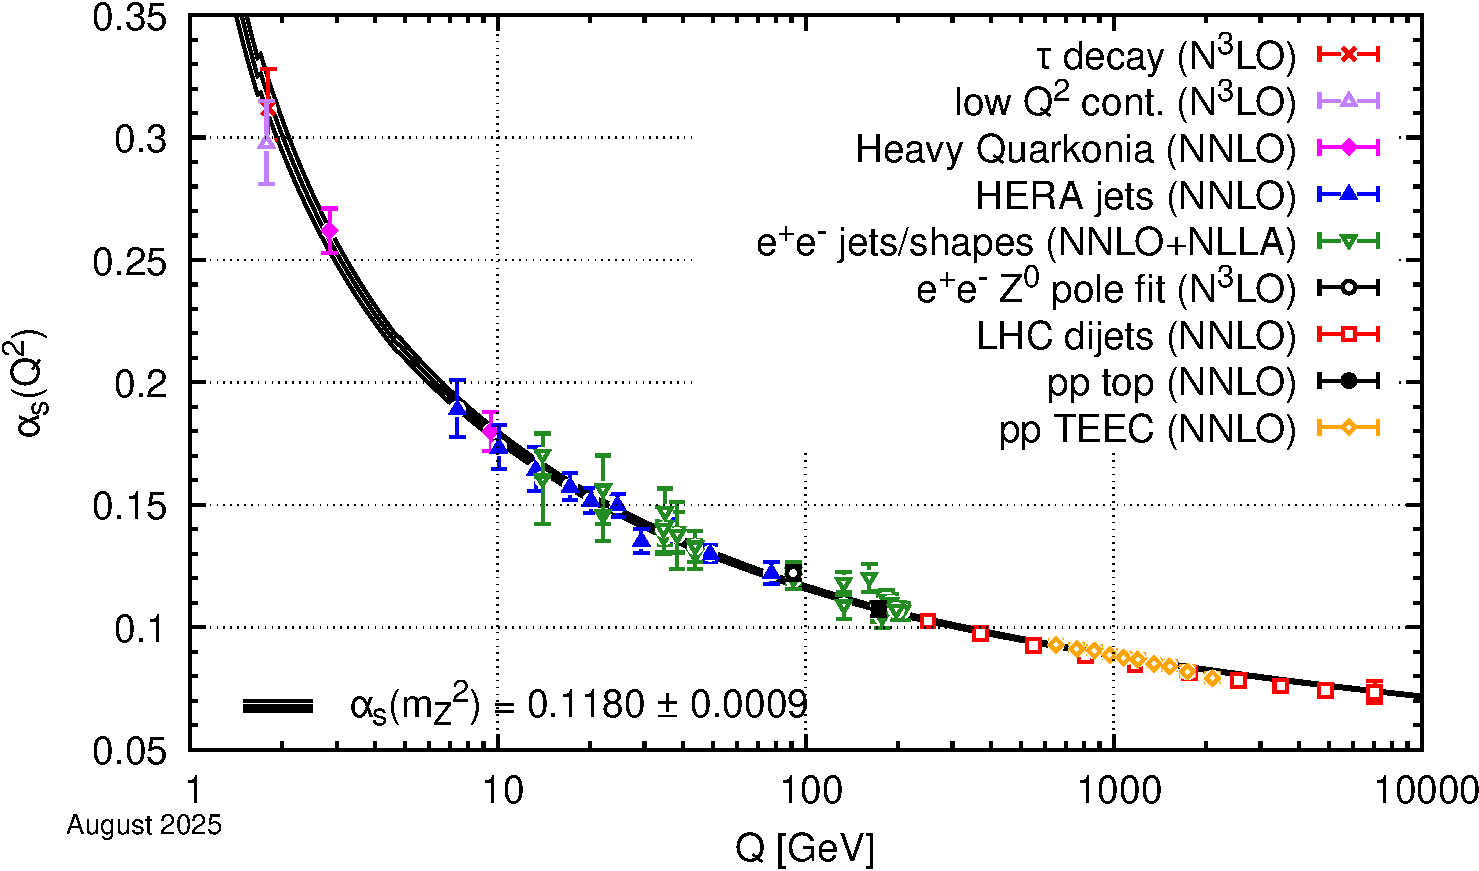
\includegraphics[width=0.7\linewidth]{figures/alphas-v-Q-2025-cropped.pdf}
	\caption{Summary of determinations of \(\alpha_s\) as a function of the energy scale Q compared to
		the running of the coupling computed at five loops taking as an input the current Particle Data Group (PDG) world average, \(\alpha_s(m_Z^2) = 0.1180 \pm 0.0009\) \cite{ParticleDataGroup:2026aaa}}
	\label{fig:runningCoupling}
\end{figure}

Integrating Eq. \ref{eq:RGEquation}
\begin{align}
	\ln(\frac{Q^2}{Q_0^2})  &= \int^{\alpha_s(Q^2)}_{\alpha_s(Q^2_0)}\frac{d\alpha_s}{\beta(\alpha_s)}\notag\\
	\implies \alpha_s(Q^2) &= \frac{\alpha_s(Q_0^2)}{1 + \beta_0(\alpha_s(Q_0^2))\ln(Q^2/Q_0^2) + \mathcal{O}(\alpha_s^2)}
	\label{eq:runningCouplingRel}
\end{align}

Usually, the reference scale \(Q_0^2\) is set to a convenient energy scale in the perturbative regime. \(\alpha_s\) at all other scales can be inferred accordingly. Usually, \(Q_0\) is set to mass of the \(Z\)-boson, \(m_Z\) as shown in Fig. \ref{fig:runningCoupling}. Another approach is to choose a scale parameter, \(\Lambda\) such that \(\alpha_s(\Lambda) \rightarrow \infty\).  

\begin{align}
	\ln(\frac{Q^2}{\Lambda^2}) &= - \int_{\alpha_s(Q^2)}^{\infty} \frac{d\alpha_s}{\beta(\alpha_s)}  \notag\\
	\implies \alpha_s(Q^2)  &= \frac{1}{\beta_0\ln(Q^2/\Lambda^2)}\left[1 - \frac{\beta_1}{\beta_0}\frac{\ln(\ln(Q^2/\Lambda^2))}{\ln(Q^2/\Lambda^2)} + \mathcal{O}\left(\frac{1}{\ln(Q^2/\Lambda^2)^2}\right)\right]
		\label{eq:runningCouplingLambda}
\end{align}

\(\Lambda\) is called the \emph{confinement scale}, around \(200~\mathrm{MeV}\). Eqs. \ref{eq:runningCouplingRel} and \ref{eq:runningCouplingLambda} show a monotonically decreasing relationship between \(\alpha_s\) and \(Q^2\). At high momentum transfers (\(Q \gg \Lambda\)), the coupling strength vanishes ($\alpha_s \to 0$). In this regime, quarks and gluons behave as quasi-free particles, making perturbative QCD (pQCD) calculations highly reliable (\emph{Asymptotic Freedom}).  At low energy scales (\(Q \ll \Lambda\)), the coupling diverges. In this non-perturbative QCD (npQCD) limit, isolated color charges cannot exist and partons are permanently bound into color-neutral hadrons (\emph{Color Confinement}).

\subsection{Quark Gluon Plasma (QGP)}
\label{sec:QGPIntro}
Asymptotic freedom of QCD means that matter at extremely high temperatures and densities (high \(Q^2\)) undergo a \emph{deconfinement} phase transition, with partonic degrees of freedom replacing hadronic degrees of freedom. 
%
This state of deconfined quarks and gluons is called QCD/quark-gluon plasma due to analogous phenomena observed in atomic physics~\cite{SHURYAK198071}.

Thermodynamically, when temperature (\(T\)) or baryon number density (\(n_\mathrm{B}\)) approaches the confinement scale \(\Lambda\) introduced in Sec.~\ref{subsec:runningCoupling} (\(T \sim \Lambda \sim \mathcal{O}(10^{12})K,~\text{and}~n_\mathrm{B} \sim \Lambda^3 \sim 1~\text{fm}^{-3}\)) the boundaries between hadrons become ill defined resulting in hadrons ``melt'' into QGP~\cite{Fukushima_2010}.  
%
For reference, the core of our sun ``only'' has \(T\sim \mathcal{O}(10^{7})K\) and \(n_\mathrm{B}\sim\mathcal{O}(10^{-14})\text{fm}^{-3}\). 

These orders of \(T\) and \(n_\mathrm{B}\) are the theorized conditions prevalent in the universe a few \(\mu\mathrm{s}\) after Big-Bang. The only natural phenomena in the present-day, cold universe that can achieve these conditions are the cores of neutron stars~\cite{Annala_2020} or neutron star mergers~\cite{neutronStarMerger}. Artificially, the required  \(T\) and \(n_\mathrm{B}\) can be achieved at facilities like the Large Hadron Collider (LHC) and Relativistic Heavy Ion Collider (RHIC) through collisions of heavy-ions (like Au, Pb, etc.) at near-light speeds, the aptly named \emph{little bangs}. More on this will be discussed in Sec. \ref{sec:heavyIonCollisions}. 

\section{Hard Processes}
To consider any nucleus as a singular coherent object, the fluctuations inside it would involve momentum transfers below the confinement scale (\(\Lambda\)) introduced in \ref{subsec:runningCoupling}, and would occur over timescales \(\sim 1/\Lambda\). We define \emph{hard-scattering processes} or just \emph{hard processes} as interactions of a hard perturbative probe with high momentum transfer \(Q >> \Lambda\). Since this interaction occurs over a time-scale \(\sim 1/Q \ll 1/\Lambda\), the perturbative probe effectively interacts with a near-static ``snapshot'' of the nucleus with a characteristic resolution \(\sim 1/Q\). 

\begin{figure}[htbp]
	\centering
	\factorizationdiagram
	\caption{Collinear factorization of a hadronic hard scattering.}
	\label{fig:factorization}
\end{figure}

Thus, the cross sections of a collision process of nuclei with momentum \(P_1\) and \(P_2\) depicted by Fig.~\ref{fig:factorization} can be \emph{factorized} into various independent components as,

\begin{equation}
	\frac{d\sigma}{d\mathbf{O}}  = \sum_{i,j,f} \int dx_1dx_2d\mathbf{\Phi}_ff_i(x_1, \mu^2)f_j(x_2, \mu^2)\frac{d\hat{\sigma}_{ij\to f}}{d\hat{\mathbf{O}}}D_f(\hat{\mathbf{O}}\to\mathbf{O}, \mu^2)
	\label{eq:factorization}
\end{equation}

Where, the interactions occur between partons \(i\) from nucleus 1 and \(j\) from nucleus 2 carrying momentum \(p_1 = x_1P_1\) and \(p_2 = x_2P_2\) respectively. \(\mu\) is an arbitrary \emph{factorization scale}, often just set to \(Q\). The \(f_{k}(x, \mu^2)\) are the \emph{parton densities} giving likelihood of a parton \(k\) to carry \(x\) fraction of it's parent nucleus's momentum at a particular factorization scale \(\mu\). \(f\) labels the partonic final state coming out of the scattering and \(\mathbf{\Phi}_f\) is its phase space. \(\hat{\sigma}_{ij\to f}\)  is the \emph{parton cross-section} for scattering of partons \(i\) and \(j\) into \(f\), kept differential in a partonic observable \(\hat{\mathbf{O}}\). We can approximate it to the \((n+k)\) order in \(\alpha_s\) as, 

\begin{equation}
	\frac{d\hat{\sigma}_{ij\to f}}{d\hat{\mathbf{O}}} = \alpha_s^k \sum_{m=0}^{n}\alpha_s^m\,\frac{d\hat{\sigma}^{(m)}_{ij\to f}}{d\hat{\mathbf{O}}}(p_1, p_2, Q^2/\mu^2)
	\label{eq:partonXsecOrders}
\end{equation}

Different hard processes will have different leading powers \(k\). \(W\) production will have \(k=0\) whereas perturbative dijet production with two outgoing quarks will have \(k=2\). 

The \(D_f(\hat{\mathbf{O}}\to\mathbf{O}, \mu^2)\) are the \emph{fragmentation functions}, giving the likelihood of a partonic final state with \(\hat{\mathbf{O}}\) being measured as \(\mathbf{O}\) once hadronization is over.
%
Like the parton densities, they cannot be calculated in perturbation theory, but they are \emph{universal}: once measured in one process they can be used in any other, and their dependence on \(\mu\) is governed by evolution equations of the same form as eq.~\ref{eq:RGEquation}.
%
Eq.~\ref{eq:factorization} is the skeleton of every measurement presented in this thesis, with the choice of \(\mathbf{O}\) being what separates one from the next, and a measurement is comparable to a calculation only if both use the same \(\mathbf{O}\).
%
Restricting \(\mathbf{O}\) to charged particles, as will be done for the angularities of Ch.~\ref{ch:angularities}, puts that restriction into \(D_f\) as well, and the non-perturbative input can then no longer be avoided.
%
The nuclear modification factors of Ch.~\ref{ch:hic} are ratios of Eq.~\ref{eq:factorization} between two collision systems, where the parton densities largely cancel and what is left is the effect of the medium on \(\hat{\sigma}_{ij\to f}\) and \(D_f\). 

%The parton densities \(f_i(x,\mu^2)\) in Eq.~\ref{eq:factorization} are not calculable in perturbation theory, but they are \emph{universal}: once measured in one process they may be used to predict any other. Requiring the physical cross section of Eq.~\ref{eq:factorization} to be independent of the arbitrary scale \(\mu\), exactly as for the coupling in Sec.~\ref{subsec:runningCoupling},
%\begin{equation}
%	\mu^2\frac{d}{d\mu^2}\,\sigma(P_1,P_2) = 0,
%	\label{eq:pdfRGE}
%\end{equation}
%ties the \(\mu\)-dependence of the densities to that of \(\hat{\sigma}_{ij}\).

\section{From partons to jets}
\label{sec:partonShower}
Outgoing partons evolve from higher to lower momentum transfer scales (say, \(t\)). Initially their evolution are modeled using the pQCD mechanism called \emph{parton shower}. Eventually, say at an infra-red scale cut-off \(t_0\), pQCD calculations stop being valid and npQCD processes like hadronization dominate. QCD Monte-Carlo programs combining parton shower at \(t < t_0\) and hadronization process at \(t > t_0\)  are called \emph{QCD event generators}


\subsection{Parton branching}
\label{subsec:dglap}
\begin{figure}[h]
\centering
\label{fig:splitKinematics}
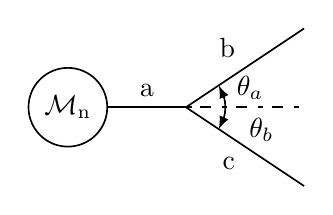
\begin{tikzpicture}[>=latex, line width=0.6pt,]
	\node[draw,circle, minimum size=1cm, inner sep=2pt] (rest) at (-1,0) {\(\mathcal{M}_\mathrm{n}\)};
	\coordinate (splitPoint) at (0.5, 0);
	\coordinate (continual) at (2,0);
	\coordinate (splitUp) at (2, 1);
	\coordinate (splitDown) at (2, -1);
	\draw (rest) to [edge label=a] (splitPoint);
	\path[draw, dash pattern=on 2pt off 3pt on 4pt off 4pt] (splitPoint) -- (continual);
	\path[draw] (splitPoint) to [edge label=b] (splitUp);
	\path[draw] (splitPoint)  to [edge label'=c] (splitDown);
	
	\pic[draw, "\(\theta_a\)",  ->, angle eccentricity=1.7] {angle = continual--splitPoint--splitUp};
	\pic[draw, "\(\theta_b\)",  <-, angle eccentricity=2.] {angle = splitDown--splitPoint--continual};
\end{tikzpicture}
\hspace{1cm}
\begin{tikzpicture}[>=latex, line width=0.6pt]
	%\node[draw,circle, minimum size=1cm, inner sep=2pt, pattern=north west lines] (rest) at (-1,0) { };
	\coordinate (incoming) at (-1, 0);
	\coordinate (splitPoint) at (0.5, 0);
	\coordinate (continual) at (2,0);
		\node[draw,circle, minimum size=1cm, inner sep=2pt] (rest) at (2,1) {\(\mathcal{M}_\mathrm{n}\)};
	\coordinate (splitDown) at (2, -1);
	\draw (incoming) to [edge label=a] (splitPoint);
	\path[draw, dash pattern=on 2pt off 3pt on 4pt off 4pt] (splitPoint) -- (continual);
	\path[draw] (splitPoint) to [edge label=b] (rest);
	\path[draw] (splitPoint)  to [edge label'=c] (splitDown);
	
	\pic[draw, "\(\theta_a\)",  ->, angle eccentricity=1.7] {angle = continual--splitPoint--splitUp};
	\pic[draw, "\(\theta_b\)",  <-, angle eccentricity=2.] {angle = splitDown--splitPoint--continual};
\end{tikzpicture}
\caption{Kinematics of timelike (left) vs spacelike (right) parton branching}
\end{figure}

Consider nearly collinear timelike splitting of a parton, \(a\to b+c\) shown in Fig. \ref{fig:splitKinematics}. Let's assume the partons are massless, and define the evolution scale (\(t\)) as, 
\begin{align}
	t \equiv p_a^2 \approx 2E_bE_c(1 - \cos\theta)  \approx z(1-z)E_a^2\theta^2
\end{align}
Where, \(z = E_b/E_a = 1 - E_c/E_a\) and \(\theta = \theta_a + \theta_b\) is the small opening angle.  The cross-section of a \(n\)-parton state branching into \(n+1\)-parton state~\cite{Ellis_Stirling_Webber_1996}
%processes can be calculated by considering \(n\)-parton matrix element.
%\begin{equation}
%	\label{eq:nPartonXsec}
%	d\sigma_n = \mathcal{F}|\mathcal{M}_n|^2d\mathbf{\Phi}_n
%\end{equation}
%
%Where \(\mathcal{F}\) is the initial-state flux factor and \(\mathbf{\Phi}_n\) is phase space of the \(n\)-parton final state. In the branching process the \(n\)-parton pre-split phase space volume element:
%
%\begin{equation}
%	d\mathbf{\Phi}_{n} = \ldots \frac{d^3\mathbf{p}_a}{2(2\pi)^3E_a}
%\end{equation}
%
%will be replaced by the \(n+1\)-parton phase space and the \(n+1\)-parton matrix element can be calculated from the \(n\)-parton matrix element. 
%\begin{align}
%	d\mathbf{\Phi}_{n+1} &= \ldots \frac{d^3\mathbf{p}_b}{2(2\pi)^3E_b} \frac{d^3\mathbf{p}_c}{2(2\pi)^3E_c} 
%	= d\mathbf{\Phi}_{n} \frac{1}{4(2\pi)^3}dtdzd\phi \notag\\
%	|\mathcal{M}_{n+1}\big|^2 &\sim \frac{8\pi\alpha_s}{t}CF|\mathcal{M}_n|^2
%\end{align}
%
%Substituting in Eq. \ref{eq:nPartonXsec} and integrating away the \(d\phi\), we get,
%
\begin{align}
	\label{eq:xsecBranching}
	%d\sigma_{n+1} &= d\sigma_n \frac{dt}{t}dz\frac{\alpha_s}{2\pi}\int\frac{d\phi}{2\pi}CF \notag\\
	d\sigma_{n+1} &= d\sigma_n \frac{dt}{t}dz\frac{\alpha_s}{2\pi} \hat{P}_{ba}
\end{align}

The \(\hat{P}_{ba}(z)\) are the \emph{unregularized Altarsi-Parisi splitting functions}, giving the probability of the branching \(a \to b + c\) with \(b\) taking a fraction \(z\) of \(a\)'s energy.
%
Their leading order forms are shown in Tab.~\ref{tab:splitfns}.
%
\(\hat{P}_{qq}\) diverges as \(z\to1\), \(\hat{P}_{gq}\) as \(z\to0\), and \(\hat{P}_{gg}\) at both ends, each of these limits being the emission of a soft gluon.
%
Only \(\hat{P}_{qg}\), the splitting of a gluon into a \(q\bar{q}\) pair, stays finite over the whole range of \(z\).
%
%This soft pole is what grooming procedures like SoftDrop (Sec.~\ref{sec:jetAlgo}) are built to remove from a measured jet.

Same equation would hold for the space-like case. 
%
To obtain the evolution equations, we can frame the evolution in terms of the change in parton distribution function \(f(x,t)\) when the evolution scale \(t\) goes from \(t\) to \(t+\delta t\),
%
\begin{align}
	\delta f_i(x, t) &= \delta f_\mathrm{in} - \delta f_\mathrm{out} \notag\\
	&=\frac{\delta t}{t} \sum_j \int_{0}^{1} dz \frac{\alpha_s}{2\pi} \left[\frac{\hat{P}_{ij}(z)}{z}f_j(x/z, t) - \hat{P}_{ji}f_i(x,t)\right]
 \end{align}
 %
The second term of the RHS gives \emph{Sudakov form factor}, which gives the probability of a parton \(i\) evolving from scale \(t\) to a softer scale \(t_0\) without a resolvable emission,
%
\begin{align}
	\Delta_i(t) \equiv \exp(-\sum_j\int_{t_0}^{t} \frac{dt^\prime}{t^\prime}\int dz\frac{\alpha_s}{2\pi} \hat{P}_{ji}(z))
\end{align}

We get the familiar DGLAP-like evolution equations,

\begin{align}
	t\frac{\partial}{\partial t}\left(\frac{f_i}{\Delta_i}\right) = \frac{1}{\Delta_i}\sum_j \int \frac{dz}{z}\frac{\alpha_s}{2\pi}
\hat{P}_{ij}(z)f_j(x/z, t)\end{align}


To deal with singularities corresponding to soft gluons at \(z\to 1\), we introduce an explicit infrared cut-off \(z < 1-\epsilon(t)\) .  Requiring the transverse momentum in timelike branching \(a\to bc\) to be positive, 
\begin{align}
	p_T^2 &= z(1-z)p_a^2 - (1-z)p_b^2 - zp_c^2 > 0 \notag\\
	\implies& z(1-z) > t_0/t \implies t_0/t < z < 1 - t_0/t
%	\implies&  z, 1-z > \epsilon(t) = \frac{1 - \sqrt{1-4t/t_0}}{2}\simeq t_0/t \notag\\
\end{align} 
and also, \(t > 2t_0\). Thus the Sudakov factors become,
%
\begin{align}
	\Delta_i(t) \equiv \exp(-\sum_j\int_{2t_0}^{t}
	\frac{dt^\prime}{t^\prime}
	\int_{t_0/t^\prime}^{1-t_0/t^\prime} dz
	\frac{\alpha_s}{2\pi} \hat{P}_{ji}(z))
	\label{eq:col`inearSudakov}
\end{align}

\subsection{Angular Ordering}
\label{sec:angularOrdering}
Sec.~\ref{subsec:dglap} took collinear enhancements into account to all orders in
\(\alpha_s\). However it does not take the enhancement in soft gluon emission at wide emission angle. 
This is demonstrated in Eq. \ref{eq:softPropagator} by considering an on-mass-shell external line of
momentum \(p\), mass \(m\) emitting a gluon with momentum \(q\)  at an angle \(\theta\)
\begin{equation}
	\frac{1}{(p\pm q)^2 - m^2} = \frac{\pm1}{2p\cdot q}
	= \frac{\pm1}{2\omega E(1-v\cos\theta)},
	\label{eq:softPropagator}
\end{equation}
where \(\omega\) is the gluon energy, \(E\) and \(v\) the energy and velocity of the
emitter and \(\theta\) the emission angle. For light partons \(v\to1\) and the
collinear enhancement appears as \(\theta\to0\); the enhancement as \(\omega\to0\)
holds for any velocity and angle. Internal lines  are off-mass-shell and carry no such enhancement, since
\((p+q)^2-m^2\to p^2-m^2\neq0\). The cross section carries a sum over all pairs of external lines \(\{i,j\}\),
\begin{align}
	\label{eq:antennaSplitXSec}
	d\sigma_{n+1}& = d\sigma_n\,\frac{d\omega}{\omega}\frac{d\Omega}{2\pi}
	\frac{\alpha_s}{2\pi}\sum_{i,j}C_{ij}W_{ij}
\end{align}
The weighted sum \(\sum_{i,j}C_{ij}W_{ij}\)  is called the \emph{antenna pattern} of the process. The \emph{color factor} \(C_{ij}\) and \emph{radiation function} \(W_{ij}\)  are defined as,
\begin{align}
	C_{ij} &= -\mathbf{Q}_i\cdot\mathbf{Q}_j  \notag \\
	W_{ij} &= \frac{\omega^2 p_i\cdot p_j}{p_i\cdot q\;p_j\cdot q}
	= \frac{1-v_iv_j\cos\theta_{ij}}
	{(1-v_i\cos\theta_{iq})(1-v_j\cos\theta_{jq})}
\end{align}
  The vectors \(\mathbf{Q}_{i}\) represents color charge of parton \(i\). 
  %\(\mathbf{Q}_i^2 = C_F\) for a quark, \(C_A\) for a gluon and \(0\) for a color singlet. 
  \begin{equation}
  	\mathbf{Q}_i^2 = 
  	\begin{cases}
  		C_F = 4/3 & i \in \text{quarks} \\[-15pt]
  		C_A = 3 & i \in \text{gluons}\\[-15pt]
  		0 & i \in \text{color singlet}
  	\end{cases}
  \end{equation}
  
  \(W_{ij}\) comes from interference between lines \(i\) and \(j\). \(W_{ij}\) can be separated into two parts  \(W^{[i/j]}_{ij}\) each with an \emph{incoherent} and a \emph{coherent} contribution from line \(i/j\)  . Assuming massless emitters (\(v_i=v_j=1\)) for simplicity,
\begin{align}
	W_{ij} &= W^{[i]}_{ij} + W^{[j]}_{ij}\notag\\
	W^{[i]}_{ij} &= \frac{1}{2}\left(\overbrace{\frac{1}{1-\cos\theta_{iq}}}^\mathrm{incoherent} + \overbrace{\frac{\cos\theta_{iq}-\cos\theta_{ij}}{(1-\cos\theta_{jq}) (1-\cos\theta_{iq})}}^\mathrm{coherent}\right)\notag\\
	&=  \frac{1}{2(1-\cos\theta_{iq})}\left(1 + \frac{\cos\theta_{iq}-\cos\theta_{ij}}{1-\cos\theta_{ij}\cos\theta_{iq} - \sin\theta_{ij}\sin\theta_{iq}\cos\phi_{iq}}\right)
	\label{eq:antennaSplit}
\end{align}
Using the direction of line \(i\) as the z-axis, \(d\Omega \)  from Eq. \ref{eq:antennaSplitXSec} becomes \(d\cos\theta_{iq}\,d\phi_{iq}\), We can carry out the \(\phi_{iq}\) integration,
\begin{align}
	\int_0^{2\pi}\frac{d\phi_{iq}}{2\pi}W^{[i]}_{ij} &= \frac{1}{1-\cos\theta_{iq}}\left(\frac{1 + \frac{\cos\theta_{iq}-\cos\theta_{ij}}{|\cos\theta_{iq}-\cos\theta_{ij}|}}{2}\right) \notag\\
	&= \begin{cases}
		\dfrac{1}{1-\cos\theta_{iq}} & \cos\theta_{iq} > \cos\theta_{ij} \implies \theta_{iq} < \theta_{ij}\\[-10pt]
		0 & \text{otherwise,}
	\end{cases}
	\label{eq:angularOrdering}
\end{align}

Eq.~\ref{eq:angularOrdering}  shows that azimuth-averaged soft gluon emission from a line \(i\) is confined to a cone, centered on \(i\)'s direction, extending up to the direction of line \(j\), \(i\)'s sibling from the preceding split. 
%
Since the emission probability of Eq.~\ref{eq:antennaSplitXSec} is weighted by the color charges, a gluon radiates \(C_A/C_F = 9/4\) times as much as a quark of the same energy into the same cone.
%
Gluon jets are therefore wider and carry more particles than quark jets of the same momentum, a difference the classifiers of Ch.~\ref{ch:methods} are trained to pick up, and one that has to be kept in mind whenever angularities are compared between samples with different quark and gluon fractions.
%The total soft gluon emission cross-section can be then easily obtained for two external lines forming a color singlet (\(e^+e^-\to q\bar{q}\)) have \(\mathbf{Q}_i+\mathbf{Q}_j=0\) and hence \(C_{q\bar{q}}=\mathbf{Q}_q^2=\mathbf{Q}_{\bar{q}}^2 = C_F\), and angular ordering suppresses radiation outside the cones extending from \(q\) to \(\bar{q}\) and vice versa.

%\begin{align}
%	d\sigma_{q\bar{q}g}& = d\sigma_{q\bar{q}}\frac{\Theta(\cos(\theta_{qg})-\cos(\theta_{q\bar{q}}))}{1-\cos\theta_{qg}}d(\cos\theta_{qg})\frac{\alpha_s}{2\pi}\frac{d\omega}{\omega}C_F
%	\label{eq:qqbarSinglet}
%\end{align}
%We will come back to Eq.~\ref{eq:qqbarSinglet} 

\subsection{Color Coherence}
\label{sec:colorCoherence}
Lets take the case of three partons \(\{i,j,k\}\) forming a color singlet (\(\mathbf{Q}_i + \mathbf{Q}_j +\mathbf{Q}_k = 0\)) e.g., \(e^+e^-\to q\bar{q} g\). First, partons \(l\) and \(k\) come from a color singlet state (\(\mathbf{Q}_l +\mathbf{Q}_k = 0\)). Then \(l\) splits into \(i\) and \(j\) (\(\mathbf{Q}_l = \mathbf{Q}_i + \mathbf{Q}_j = -\mathbf{Q}_k\)). The antennae function for this state is:
\begin{align}
		\label{eq:threePartonW}
  \sum_{a,b}C_{ab}W_{ab} &= -\mathbf{Q}_i\!\cdot\!\mathbf{Q}_jW_{ij} -\mathbf{Q}_j\!\cdot\!\mathbf{Q}_kW_{jk} -\mathbf{Q}_i\!\cdot\!\mathbf{Q}_kW_{ik} \notag\\
	&= \frac{1}{2}\left[\mathbf{Q}_i^2(W_{ij} + W_{ik} - W_{jk}) + \mathbf{Q}_j^2(W_{ij} + W_{jk} - W_{ik}) + \mathbf{Q}_k^2(W_{ik} + W_{jk} - W_{ij})\right]\notag\\
	&=\mathbf{Q}_i^2\left(W_{ij}^{[i]} + \tilde{W}_{jk}^{[i]} - \tilde{W}_{ik}^{[j]}\right) + \mathbf{Q}_j^2\left(W_{ij}^{[j]} + \tilde{W}_{ik}^{[j]} - \tilde{W}_{jk}^{[i]}\right) \notag\\
	& + \mathbf{Q}_k^2\left(\tilde{W}_{jk}^{[i]} + \tilde{W}_{ik}^{[j]} + \frac{W_{ik}^{[k]} + W_{jk}^{[k]} }{2}\right)
\end{align}
Where,
\begin{equation}
	\tilde{W}_{jk}^{[i]} = \frac{W^{[i]}_{ik} - W^{[i]}_{ij}}{2},\quad \tilde{W}_{ik}^{[j]} = \frac{W^{[j]}_{jk} - W^{[j]}_{ij}}{2}
\end{equation}
are shifted radiation functions for lines \(i\) and \(j\), with the collinear singularity canceled out. This allows us to make certain useful approximations. Taking \(\theta_{ij}\to0\), we can approximate the directions of \(i\) and \(j\) by \(l\). 
\begin{align}
	W_{ik}^{[k]} \simeq W_{jk}^{[k]} \simeq W_{lk}^{[k]},\text{and}~\tilde{W}_{jk}^{[i]} \simeq \tilde{W}_{ik}^{[j]} \simeq W_{lk}^{[ij]}/2 
\end{align}
Where, 
\begin{equation}
	\tilde{W}^{[ij]}_{lk} = \begin{cases}
		W^{[l]}_{lk} & \theta_{lq}>\theta_{ij}\\[-10pt]
		0            & \theta_{lq}<\theta_{ij},
	\end{cases}
\end{equation}
\begin{equation}
	W \simeq \mathbf{Q}_i^2W^{[i]}_{ij} + \mathbf{Q}_j^2W^{[j]}_{ij}
	+ \mathbf{Q}_k^2W^{[k]}_{lk} + \mathbf{Q}_l^2\tilde{W}^{[ij]}_{lk},
	\label{eq:coherentPattern}
\end{equation}

\begin{figure}[htbp]
	\centering
	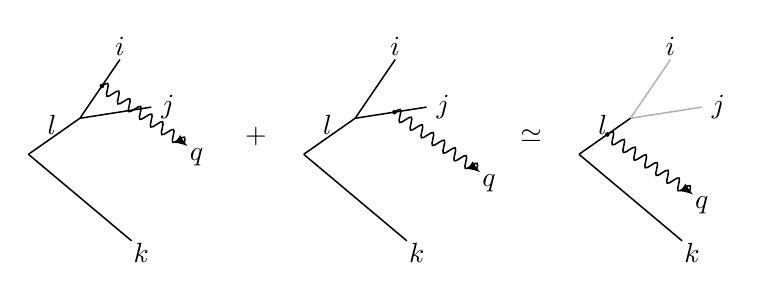
\begin{tikzpicture}[line width=0.55pt, scale=0.76,
		gl/.style={decorate, decoration={coil, aspect=0, segment length=1.7mm,
				amplitude=0.7mm}, ->}]
		
		\begin{scope}[xshift=0cm]
			\coordinate (o) at (0,0);
			\coordinate (l) at (35:1.05);
			\coordinate (i) at (46:2.2);
			\coordinate (j) at (21:2.2);
			\coordinate (k) at (-40:2.25);
			\draw[black] (l) -- (i) node[black, above=-2pt] {\(i\)};
			\draw[black] (l) -- (j) node[black, right=0pt] {\(j\)};
			\draw (o) -- node[above left=-5pt, pos=0.55] {\(l\)} (l);
			\draw (o) -- (k) node[below right=-4pt] {\(k\)};
			\coordinate (e) at ($(l)!0.55!(i)$);
			\fill (e) circle (1.1pt);
			\draw[gl] (e) -- ($(e)+(-35:1.75)$) node[below right=-4pt] {\(q\)};
			%\node at (1.1,-2.1) {\(\mathcal{M}_i\)};
		\end{scope}
		
		\node at (3.8,0.3) {\(+\)};
		
		\begin{scope}[xshift=4.6cm]
			\coordinate (o) at (0,0);
			\coordinate (l) at (35:1.05);
			\coordinate (i) at (46:2.2);
			\coordinate (j) at (21:2.2);
			\coordinate (k) at (-40:2.25);
			\draw[black] (l) -- (i) node[black, above=-2pt] {\(i\)};
			\draw[black] (l) -- (j) node[black, right=0pt] {\(j\)};
			\draw (o) -- node[above left=-5pt, pos=0.55] {\(l\)} (l);
			\draw (o) -- (k) node[below right=-4pt] {\(k\)};
			\coordinate (e) at ($(l)!0.55!(j)$);
			\fill (e) circle (1.1pt);
			\draw[gl] (e) -- ($(e)+(-35:1.75)$) node[below right=-4pt] {\(q\)};
			%\node at (1.1,-2.1) {\(\mathcal{M}_j\)};
		\end{scope}
		
		\node at (8.4,0.3) {\(\simeq\)};
		
		\begin{scope}[xshift=9.2cm]
			\coordinate (o) at (0,0);
			\coordinate (l) at (35:1.05);
			\coordinate (i) at (46:2.2);
			\coordinate (j) at (21:2.2);
			\coordinate (k) at (-40:2.25);
			\draw[black!30] (l) -- (i) node[black, above=-2pt] {\(i\)};
			\draw[black!30] (l) -- (j) node[black, right=0pt] {\(j\)};
			\draw (o) -- node[above left=-5pt, pos=0.55] {\(l\)} (l);
			\draw (o) -- (k) node[below right=-4pt] {\(k\)};
			\coordinate (e) at ($(o)!0.55!(l)$);
			\fill (e) circle (1.1pt);
			\draw[gl] (e) -- ($(e)+(-35:1.75)$) node[below right=-4pt] {\(q\)};
			%\node at (1.1,-2.1) {\(\mathcal{M}_l\)};
		\end{scope}
	\end{tikzpicture}
	\caption{Wide-angle emission of soft gluon \(q\), off \(i\) and \(j\), acts as if
	the emission came off the parent parton \(l\), imagined to be on shell.}
	\label{fig:threeParton}
\end{figure}


Each parton radiates in proportion to its color charge squared. When \(i\) and \(j\) close in angle their incoherent
contributions are limited to cones of half-angle \(\theta_{ij}\), while at larger
angles, out to the direction of \(k\), they radiate coherently in proportion to
their combined charge \(\mathbf{Q}_l^2\), as if from an internal line of momentum
\(p_l = p_i+p_j\) as shown in Fig.~\ref{fig:threeParton}.

\subsection{Coherent Parton Branching}
\label{sec:coherentPartonBranching}
Extended to higher orders this gives a \emph{coherent parton branching} formalism.
In place of the virtual mass-squared \(t\) the evolution variable is the opening
angle, or more precisely
\begin{equation}
	\zeta = \frac{p_b\cdot p_c}{E_bE_c} \simeq 1-\cos\theta
	\label{eq:zeta}
\end{equation}
for \(a\to bc\), with angular ordering \(\zeta^\prime<\zeta\) imposed on successive
branchings and the propagator factor \(dt/t\) of Sec.~\ref{subsec:dglap} replaced by
\(d\zeta/\zeta\). Using the splitting function \(\hat{P}_{ba}(z)dz\) rather than the
soft approximation \(\mathbf{Q}_a^2d\omega/\omega\) treats both soft and collinear
enhancements correctly, so that
\begin{equation}
	d\sigma_{n+1} = d\sigma_n\,\frac{d\zeta}{\zeta}\,dz\,
	\frac{\alpha_s}{2\pi}\hat{P}_{ba}(z).
	\label{eq:coherentBranching}
\end{equation}
The virtual mass-squared cut-off is replaced by an angular one,
\(\zeta_0 = t_0/E^2\) for a parton of energy \(E\), and the convenient evolution
variable \(\tilde{t} = E^2\zeta \geq t_0\) in terms of which the ordering condition \(\zeta_b,\zeta_c<\zeta_a\) and the
resulting cut-off on \(z\) read
\begin{equation}
	\tilde{t}_b < z^2\tilde{t},
	\qquad
	\tilde{t}_c < (1-z)^2\tilde{t},
	\qquad
	\sqrt{t_0/\tilde{t}} < z < 1-\sqrt{t_0/\tilde{t}} ,
	\label{eq:orderingCutoff}
\end{equation}
with \(\tilde{t}=\tilde{t}_a\) and \(z=E_b/E_a\). Neglecting the masses of \(b\) and
\(c\),
\begin{equation}
	t = z(1-z)\tilde{t},
	\qquad
	p_t^2 = z^2(1-z)^2\tilde{t},
	\label{eq:tAndPt}
\end{equation}
and the Sudakov form factor of Sec.~\ref{subsec:dglap} becomes
\begin{align}
	\tilde{\Delta}_i(\tilde{t}) \equiv \exp(-\sum_j\int_{4t_0}^{\tilde{t}}
	\frac{d\tilde{t}^\prime}{\tilde{t}^\prime}
	\int_{\sqrt{t_0/\tilde{t}^\prime}}^{1-\sqrt{t_0/\tilde{t}^\prime}} dz
	\frac{\alpha_s(z^2(1-z)^2\tilde{t}^\prime)}{2\pi} \hat{P}_{ji}(z))
	\label{eq:coherentSudakov}
\end{align}

At large \(\tilde{t}\) this falls more slowly than its collinear counterpart, though
still faster than any negative power of \(\tilde{t}\). The slower fall implies less
branching, which is the suppression of soft gluon emission by angular ordering.

\subsection{Angular structure of a jet}
\label{sec:angularityEstimate}
Sec.~\ref{sec:coherentPartonBranching} is enough to estimate what the radiation around a hard parton looks like. 
%
At a hadron collider, the angle \(\theta\) between two particles is measured as their distance \(\Delta R\) in the \etaphi plane and the energy \(E\) as the transverse momentum \(p_\mathrm{T}\) (see Sec.~\ref{sec:detCoordSys}), and a \emph{jet} is, for now, all the radiation within \(\Delta R < R\) of the initiating parton. 
%
Taking \(z\) to be the momentum fraction of the emitted gluon, as in \(\hat{P}_{gq}\) and \(\hat{P}_{gg}\) of Tab.~\ref{tab:splitfns}, the soft limit is \(\hat{P}_{gi}(z) \to 2C_i/z\) and \(d\zeta/\zeta \to 2d\theta/\theta\), so Eq.~\ref{eq:coherentBranching} becomes,
\begin{equation}
	dP = \frac{2\alpha_s C_i}{\pi}\frac{d\hat{\theta}}{\hat{\theta}}\frac{dz}{z}, \qquad \hat{\theta} \equiv \frac{\Delta R}{R} < 1
	\label{eq:lundDensity}
\end{equation}
Where, \(C_i = \mathbf{Q}_i^2\) is the color charge of the initiating parton from Sec.~\ref{sec:angularOrdering}. 
%
Eq.~\ref{eq:lundDensity} is flat in \(\ln(1/z)\) and \(\ln(1/\hat{\theta})\), so a jet is filled uniformly in this plane, the \emph{Lund plane}, down to the cut-off. 
%
The \emph{generalized angularity} of a jet is the sum over its emissions,
\begin{equation}
	\lambda_\beta = \sum_{i \in \mathrm{jet}} z_i\,\hat{\theta}_i^{\,\beta}
	\label{eq:angularityShower}
\end{equation}
Eq.~\ref{eq:LambdaKappaBeta} is the same quantity written in terms of the measured constituents of a jet, with \(z_i \to p_\mathrm{T, const}/p_\mathrm{T, jet}\) and \(\hat{\theta}_i \to \Delta R_\mathrm{const, jet}/R\), and with a second exponent \(\kappa\) on \(z_i\) which is \(1\) here. 
%
For \(\beta > 0\), an emission contributes nothing to \(\lambda_\beta\) in either the soft or the collinear limit, which is what makes it an IRC safe observable. 
%
Since \(\lambda_\beta\) is additive, the probability of a jet having an angularity below \(\hat{\lambda}_\beta\) is the probability of no emission with \(z\hat{\theta}^\beta > \hat{\lambda}_\beta\), which is the Sudakov form factor of Eq.~\ref{eq:coherentSudakov} with the no-emission condition replaced accordingly. 
%
Calling this cumulative distribution \(\Sigma_i(\hat{\lambda}_\beta)\), with the hat marking it as a parton level quantity like in Eq.~\ref{eq:factorization}, the hadron level cross section follows from it through the fragmentation function of Eq.~\ref{eq:factorization} for \(\mathbf{O} = \lambda_\beta\), summed over the flavor of the parton initiating the jet,
\begin{align}
	\frac{d\sigma}{d\lambda_\beta} &= \sum_{i \in \{q, g\}}\int d\hat{\lambda}_\beta\,\frac{d\sigma_i}{d\hat{\lambda}_\beta}\,D_i(\hat{\lambda}_\beta \to \lambda_\beta) = \sum_{i \in \{q, g\}}\sigma_i\int d\hat{\lambda}_\beta\,\frac{d\Sigma_i}{d\hat{\lambda}_\beta}\,D_i(\hat{\lambda}_\beta \to \lambda_\beta)
	\label{eq:angularityCumulant}
\end{align}
Where, \(\sigma_i\) is the cross section for producing a jet initiated by parton \(i\), i.e. Eq.~\ref{eq:factorization} with everything but the flavor of the outgoing parton integrated over, and \(d\sigma_i/d\hat{\lambda}_\beta = \sigma_i\,d\Sigma_i/d\hat{\lambda}_\beta\) is its parton level distribution. 
%
Normalized to the total cross section, the left hand side is the distribution measured in Ch.~\ref{ch:angularities}. 
%
The rest of this section is about \(\Sigma_i\), and comes back to \(D_i\) at the end. 
%
At fixed coupling,
\begin{align}
	\Sigma_i(\hat{\lambda}_\beta) &= \exp\left(-\frac{2\alpha_s C_i}{\pi}\int_0^1\frac{d\hat{\theta}}{\hat{\theta}}\int_0^1\frac{dz}{z}\,\Theta(z\hat{\theta}^\beta - \hat{\lambda}_\beta)\right) \notag\\
	&= \exp\left(-\frac{\alpha_s C_i}{\pi\beta}\ln^2\hat{\lambda}_\beta\right)
	\label{eq:angularitySudakov}
\end{align}
Quark and gluon jets differ only through \(C_i\), so \(\Sigma_g = \Sigma_q^{C_A/C_F}\)~\cite{Larkoski_2014}.
%
 A convenient choice for scale of \(\alpha_s\) is \(p_\mathrm{T, jet}R\), the largest transverse momentum an emission inside the jet can have. 
%

Tab.~\ref{tab:angularityEstimate} evaluates Eq.~\ref{eq:angularitySudakov} for the three \(\beta\) values measured in Ch.~\ref{ch:angularities}. 

\begin{table}[htbp]
	\centering
	\begin{tabular}{c c c c c}
		\toprule
		\multirow{2}{*}{\(\beta\)} & \multicolumn{2}{c}{median \(\hat{\lambda}_\beta\)} & \multicolumn{2}{c}{fraction with \(\hat{\lambda}_\beta > 0.1\)} \\
		\cmidrule(lr){2-3} \cmidrule(lr){4-5}
		 & quark & gluon & quark & gluon \\
		\midrule
		0.5 & 0.13  & 0.26  & 59\% & 87\% \\
		1   & 0.06  & 0.15  & 36\% & 64\% \\
		2   & 0.02  & 0.07  & 20\% & 40\% \\
		\bottomrule
	\end{tabular}
	\caption[Leading logarithmic estimates of jet angularities at RHIC]{Parton level median angularity and fraction of jets with \(\hat{\lambda}_\beta > 0.1\) from Eq.~\ref{eq:angularitySudakov} at \(\alpha_s = 0.2\), corresponding to \(p_\mathrm{T, jet} \approx 20~\mathrm{GeV}/c\) and \(R = 0.4\), for quark (\(C_F = 4/3\)) and gluon (\(C_A = 3\)) initiated jets.}
	\label{tab:angularityEstimate}
\end{table}

Median angularities are larger by  a factor of 2--3 for gluon jets compared to quark jets. 
%
Increasing \(\beta\) pushes both to smaller values and widens the gap between them, as the observable weighs the wide angle radiation more heavily. 
%
Going up in \(p_\mathrm{T, jet}\) only changes \(\alpha_s\) logarithmically, so the distributions are expected to narrow slowly. 

%Eq.~\ref{eq:lundDensity} only holds for emissions whose transverse momentum, \(k_\mathrm{T} \approx z\,p_\mathrm{T, jet}\Delta R\), is above the scale where \(\alpha_s\) stops being perturbative, and below it the emissions are replaced by hadronization, which is what \(D_i\) in Eq.~\ref{eq:angularityCumulant} accounts for. 
%%
%An emission with \(k_\mathrm{T}\) between \(\Lambda \approx 0.2\)~GeV and \(1\)~GeV sitting at the edge of the jet contributes \(k_\mathrm{T}/(p_\mathrm{T, jet}R) \approx 0.03\)--\(0.12\) to \(\lambda_\beta\) for any \(\beta\), which is as large as the medians of Tab.~\ref{tab:angularityEstimate}. 
%%
%Thus at RHIC energies the npQCD part of an angularity is not a small correction on top of the pQCD part, and it only falls as \(1/p_\mathrm{T, jet}\). 
%%
%This is why the angularity distributions measured in Ch.~\ref{ch:angularities} sit above these estimates by about this much, why removing the soft wide angle radiation by grooming (Sec.~\ref{sec:jetAlgo}) brings them closer, and why the event generators of Sec.~\ref{sec:eventGenerators} are tested there as much on their hadronization as on their showers. 
%
%These are leading logarithmic estimates at fixed coupling, and are indicative rather than predictions. 
%%
%Terms of order \(\alpha_s\ln(1/\lambda_\beta)\), coming from the running of \(\alpha_s\), hard collinear splittings, the recoil of the jet axis against the emissions for \(\beta \leq 1\), and radiation across the jet boundary, are all of order one half at these values. 
%%
%The angularities with \(\kappa \neq 1\) used for \AuAu collisions in Ch.~\ref{ch:angularities} are not IRC safe, and no estimate of this kind exists for them. 

\section{Hadronization and event generators}
\label{sec:eventGenerators}
Coherent branching does not only suppress soft emission, it also organizes the color flow of the shower.
%
Eq.~\ref{eq:coherentPattern} of shows that a pair of partons close in angle radiates as its parent, carrying the parent's charge, so the color of a branching is handed down the tree along with its momentum.
%
Applying this at every branching down to the cut-off \(t_0\), neighbouring partons are the ones that are color connected, and the final state has sorted itself into color singlet groups whose invariant masses are set by \(t_0\) and \(\Lambda\), and not by the scale of the hard process that started it.
%
This property is called \emph{preconfinement}~\cite{Ellis_Stirling_Webber_1996}.
%
The preconfined singlets can either decay directly into hadrons, giving the \emph{cluster} models~\cite{Webber:147786}, or stretch a confining color flux tube between color connected partons and break it up, giving the \emph{string} models~\cite{ANDERSSON198331}. 

QCD event generators chain these processes, matrix elements for the hard processes from eq.~\ref{eq:factorization}, parton showers, additional semi-hard scatterings among the remaining constituents of the incoming hadrons making up the \emph{underlying event}, hadronization, and finally the decays of unstable hadrons.
%
Everything below the hard process carries parameters that are not fixed by theory, and a set of values for them obtained by fitting to data is called a \emph{tune}.
%
Two generators starting from the same matrix element can therefore still disagree, and the spread between them is the usual way of gauging how much of a prediction is genuinely perturbative. 

This thesis uses PYTHIA~\cite{Sj_strand_2006} and HERWIG~\cite{Bellm:2015jjp}, which differ in how they deal with the coherence of Sec.~\ref{sec:coherentPartonBranching}.
%
HERWIG orders its shower in angle and imposes Eq.~\ref{eq:angularOrdering} directly, then hadronizes the preconfined singlets as clusters.
%
PYTHIA instead orders in transverse momentum and radiates off color dipoles rather than off individual partons, which suppresses soft wide-angle emission without ordering in angle at all, and hadronizes with strings.
%

Both generators are used with tunes made for RHIC energies~\cite{Skands_2010, PhysRevD.105.016011, adkins2019studying}, as the tunes in widest use are fitted mostly to LHC data and overshoot the underlying event at \sPP{200}{GeV}.
%
PYTHIA-6 and PYTHIA-8 share the string hadronization and the transverse-momentum ordered shower, and differ mainly in their treatment of multiple parton interactions, color reconnection and beam remnants, all of which control the multiplicity and the soft, wide-angle part of an event.
%

Ch.~\ref{ch:jhcorr} also uses JEWEL~\cite{Zapp:2013vla}, which adds scattering of the shower partons off a thermal medium to this picture.
%
The response of the detector to the generated particles is simulated separately using GEANT~\cite{Brun:1987ma}, and Ch.~\ref{ch:methods} describes how its effects are taken back out of a measurement.


\section{Outline of this thesis}
Angular ordering makes the angular distribution of energy inside a jet a record of the shower that produced it, with the wide-angle radiation coming from the early, hard splittings and the core of the jet being filled in later.
%
This thesis measures that distribution.
%
It is measured first in \pp collisions, where it is a test of the vacuum shower and a baseline, and then in \AuAu collisions, where a deviation from that baseline is the imprint of the medium the shower has gone through. 

Ch.~\ref{ch:STAR} describes RHIC and the STAR detector, in particular the TPC and the BEMC which measure the charged and neutral parts of a jet.
%
Ch.~\ref{ch:hic} defines jets as the output of a jet finding algorithm rather than as partons, introduces SoftDrop grooming, and sets up the quantities used to describe a heavy-ion collision: the Glauber picture of the initial state, centrality, the event plane, and the nuclear modification factors used to quantify jet quenching.
%
Ch.~\ref{ch:methods} collects the analysis techniques, mainly the classifiers used to tag jets and the unfolding procedure used to remove detector effects from a measured distribution.
%
Ch.~\ref{ch:jhcorr} presents jet-hadron correlations relative to the event plane in \AuAu collisions, which probe the dependence of energy loss on the path length traversed in the medium.
%
Ch.~\ref{ch:angularities} presents generalized angularities, inclusive and groomed, in \pp collisions and then in \AuAu collisions.
%
Ch.~\ref{ch:summary} summarizes both measurements and what they suggest about where to go next. 

%% =====================================================================
%  qgmutualinfo.tex -- A. J. Larkoski, J. Thaler, W. J. Waalewijn,
%  "Gaining (Mutual) Information about Quark/Gluon Discrimination",
%  JHEP 11 (2014) 129 [arXiv:1408.3122], recast in the notation of
%  chapters/intro.tex and chapters/angularities.tex.
%
%  WHERE IT GOES: as a section either at the end of Sec. 1.4
%  (sec:partonShower), after jetportrait.tex, or as the opening
%  theory section of Ch. \ref{ch:angularities}.  It is written as a
%  \section with \subsections, matching jetportrait.tex.
%
%  NOTATION MAP -- paper -> thesis:
%    \lambda^\kappa_\beta   -> same symbol, Eq. \ref{eq:LambdaKappaBeta}
%    e_\beta = \lambda^1_\beta -> written \lambda^1_\beta throughout
%    C_i (C_F, C_A)         -> \mathbf{Q}_i^2, intro.tex Sec. 1.4.2
%    \theta_i = R_i/R_0     -> \Delta R_{const,jet}/R
%    \Sigma_i(e)            -> \Sigma_i(\lambda), same
%    their \beta_0, \beta_1 -> the thesis' \beta_0 (eq:RGEquation)
%    P_{i\to ig}(z)         -> \hat{P}_{gi}(z), Table \ref{tab:splitfns}
%
%  LABELS ASSUMED TO EXIST (all currently live):
%    ch:intro, ch:angularities, sec:partonShower, subsec:dglap,
%    sec:coherentPartonBranching, tab:splitfns, eq:antennaSplitXSec,
%    eq:angularOrdering, eq:coherentSudakov, eq:runningCouplingLambda,
%    eq:RGEquation, eq:LambdaKappaBeta, fig:GroomingAndRg
%
%  IF jetportrait.tex IS UNCOMMENTED in intro.tex, three derivations
%  below become one-line callbacks instead:
%    eq:qgmiLLsudakov  == jetportrait's eq:angularitySudakov
%    the (u,v) plane   == jetportrait's Eq. (angularityDef), 2nd line
%    9/4 and delta_g   == jetportrait's eq:casimirRatio, eq:swWidth
%  I have kept them self-contained here, with a pointer, so the file
%  compiles against intro.tex as it stands today.  Labels are all
%  prefixed eq:qgmi.../fig:qgmi... so nothing collides with
%  jetportrait.tex or qgjets.tex.
%
%  BIBTEX: \cite{Larkoski_2014} already resolves -- but thesis.bib
%  contains THREE identical Larkoski_2014 entries (lines 101, 268,
%  3092).  BibTeX takes the first and warns on the rest; worth
%  deduplicating at some point.  Not touched here.
% =====================================================================

\section{Quark--gluon discrimination as an information problem}
\label{sec:qgmi}

Chapter~\ref{ch:intro} ended with a cascade whose every emission rate is
proportional to the squared colour charge \(\mathbf{Q}_i^2\) of whatever is
radiating. That single fact is the whole of quark--gluon discrimination at lowest
order, and it is also its ceiling. The purpose of this section is to make that
statement quantitative, following Larkoski, Thaler and
Waalewijn~\cite{Larkoski_2014}, who ask two questions that the cascade alone does
not answer: \emph{how much} separation does \(\mathbf{Q}_g^2/\mathbf{Q}_q^2=9/4\)
actually buy, and \emph{what has to be true} of an observable for it to do better.
The answers are, respectively, about a tenth of one bit, and that the observable
must resolve something in the jet other than its overall colour charge.

\subsection{The observable family, in the variables of Chapter~\ref{ch:intro}}
\label{subsec:qgmiFamily}

The paper's discriminants are exactly the generalized angularities of
Eq.~\ref{eq:LambdaKappaBeta},
\begin{equation}
	\lambda^\kappa_\beta = \sum_{c\,\in J} z_c^\kappa\,\theta_c^\beta ,
	\qquad
	z_c = \frac{p_{\mathrm{T},c}}{\sum_{c^\prime\in J}p_{\mathrm{T},c^\prime}} ,
	\qquad
	\theta_c = \frac{\Delta R_{c}}{R} ,
	\label{eq:qgmiAngularity}
\end{equation}
with \(0\le z_c,\theta_c\le1\) and both exponents non-negative. A single
two-parameter family contains most of the observables the quark--gluon literature
uses, at the four corners of Fig.~\ref{fig:qgmiLambdaSpace}: \(\lambda^0_0\) is
constituent multiplicity, \(\lambda^2_0\) is \(p_T^D\), \(\lambda^1_1\) is the jet
width (girth, broadening), and \(\lambda^1_2\) is thrust, i.e.\ jet mass squared
over energy squared. Raising \(\beta\) weights wide-angle radiation, raising
\(\kappa\) weights hard constituents; \(\beta\) reaches into the cascade's angular
ordering and \(\kappa\) into its energy sharing, and these are the two independent
handles Sec.~\ref{sec:coherentPartonBranching} provides.

\begin{figure}[htbp]
	\centering
	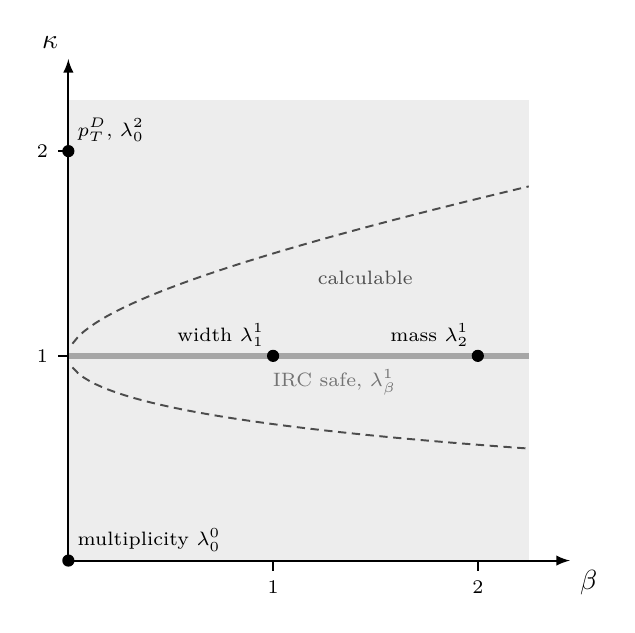
\begin{tikzpicture}[x=2.6cm, y=2.6cm, line width=0.7pt]
		\fill[black!7] (0,0) rectangle (2.25,2.25);
		% IRC-safe line kappa = 1
		\draw[line width=2.2pt, black!35] (0,1) -- (2.25,1);
		\node[black!55, font=\scriptsize] at (1.30,0.87)
		{IRC safe, \(\lambda^1_\beta\)};
		\draw[->] (0,0) -- (2.45,0) node[below right] {\(\beta\)};
		\draw[->] (0,0) -- (0,2.45) node[above left] {\(\kappa\)};
		\foreach \i in {1,2} {
			\draw (\i,0) -- (\i,-0.05) node[below] {\scriptsize\(\i\)};
			\draw (0,\i) -- (-0.05,\i) node[left] {\scriptsize\(\i\)};
		}
		\foreach \p/\l/\a in {%
			{0,0}/{multiplicity \(\lambda^0_0\)}/{above right},
			{0,2}/{\(p_T^D\), \(\lambda^2_0\)}/{above right},
			{1,1}/{width \(\lambda^1_1\)}/{above left},
			{2,1}/{mass \(\lambda^1_2\)}/{above left}} {
			\fill (\p) circle (2.2pt);
			\node[\a, font=\scriptsize, inner sep=3pt] at (\p) {\l};
		}
		% edge of the calculable region: 6(1-kappa)^2 = beta*kappa, i.e.
		% kappa = [(12+beta) +- sqrt((12+beta)^2-144)]/12
		\draw[densely dashed, black!70] plot[domain=0.02:2.25, samples=80]
		(\x, {((12+\x) - sqrt((12+\x)*(12+\x)-144))/12});
		\draw[densely dashed, black!70] plot[domain=0.02:2.25, samples=80]
		(\x, {((12+\x) + sqrt((12+\x)*(12+\x)-144))/12});
		\node[font=\scriptsize, black!70] at (1.45,1.38) {calculable};
	\end{tikzpicture}
	\caption[The space of generalized angularities]{%
		The \((\beta,\kappa)\) plane of Eq.~\ref{eq:qgmiAngularity}. The line
		\(\kappa=1\) holds the IRC safe angularities; the four marked points are the
		observables in common use. Inside the dashed contour,
		\(\beta\kappa/(1-\kappa)^2>6\) of Eq.~\ref{eq:qgmiBarrier}, the distribution
		is calculable from the cascade with a single non-perturbative number; outside
		it, an entire non-perturbative function is needed. Redrawn from
		Ref.~\cite{Larkoski_2014}.}
	\label{fig:qgmiLambdaSpace}
\end{figure}

Two features of Eq.~\ref{eq:qgmiAngularity} carry consequences that are easy to
miss and that both bear on Chapter~\ref{ch:angularities}.

\paragraph{Infrared and collinear safety sits at \(\kappa=1\) only.} Splitting a
constituent of momentum fraction \(z\) into two collinear pieces \(z_1+z_2=z\)
changes \(\sum z_c^\kappa\) by \(z_1^\kappa+z_2^\kappa-z^\kappa\), which vanishes
only for \(\kappa=1\). The \(\beta>0\) suppression handles the collinear region at
the \emph{jet axis} but not collinear splittings of a wide-angle constituent, so
\(\kappa\neq1\) is collinear unsafe everywhere in \(\beta\). This is the same
statement as the one made after Eq.~\ref{eq:LambdaKappaBeta}: restricting the sum
to charged tracks is a \(\kappa\)-like reweighting and costs IRC safety.
Sec.~\ref{subsec:qgmiUnsafe} is the machinery that buys it back.

\paragraph{The axis must be recoil-free.} Ref.~\cite{Larkoski_2014} measures
\(\Delta R_c\) to the \emph{winner-take-all} axis, not to the jet momentum axis.
The distinction is invisible at \(\beta\ge1\) but not below: with a momentum axis, a
single hard wide-angle emission displaces the axis itself, so \(\lambda^\kappa_\beta\)
measures the recoil of the initiating parton rather than the radiation pattern about
it, and the resummation acquires a second, spurious source of logarithms. Every
analytic statement below assumes a recoil-free axis. The measurement in
Chapter~\ref{ch:angularities} uses the standard jet axis, so the calculations quoted
here are a guide to the physics rather than a prediction to be overlaid on the data
--- unless the axis is changed.

The one kinematic picture used throughout is the cascade's own. Eq.~\ref{eq:antennaSplitXSec}
in the soft-collinear limit gives a single emitter the emission density
\begin{equation}
	dn = \frac{2\alpha_s\mathbf{Q}_i^2}{\pi}\frac{dz}{z}\frac{d\theta}{\theta}
	= \frac{2\alpha_s\mathbf{Q}_i^2}{\pi}\,du\,dv ,
	\qquad
	u = \ln\frac{1}{z} ,
	\qquad
	v = \ln\frac{1}{\theta} ,
	\label{eq:qgmiLundPlane}
\end{equation}
uniform on the quadrant \(u,v>0\) with a density set entirely by \(\mathbf{Q}_i^2\).
An emission contributes \(z^\kappa\theta^\beta = e^{-(\kappa u+\beta v)}\) to
Eq.~\ref{eq:qgmiAngularity}, so \(\lambda^\kappa_\beta>\lambda\) requires an emission
below the straight line \(\kappa u+\beta v=\ln(1/\lambda)\). Every result in this
section is a statement about that line and about the uniform density it cuts.

\subsection{Truth overlap: the right way to score a discriminant}
\label{subsec:qgmiMI}

The paper's organising quantity is the \emph{mutual information} between two
variables,
\begin{equation}
	I(A;B) = \int da\,db\;p(a,b)\log_2\frac{p(a,b)}{p(a)p(b)}
	= H(A)+H(B)-H(A,B) ,
	\label{eq:qgmiMIdef}
\end{equation}
with \(H\) the Shannon entropy, \(H(A)=-\sum_a p(a)\log_2p(a)\). Written the second
way it is manifestly the overlap area of two sets in Fig.~\ref{fig:qgmiVenn}:
\(H(A)\) and \(H(B)\) are the number of bits each variable carries, \(H(A,B)\) the
number the two carry together, and \(I(A;B)\) the bits they share. It vanishes iff
\(a\) and \(b\) are independent.

Now let \(T\) be the jet's flavour, \(t=0\) for a quark and \(t=1\) for a gluon, and
take a sample that is half of each, so that \(H(T)=1\): there is exactly one bit of
truth to be recovered, no matter how many bits an observable carries in total. The
\emph{truth overlap} of an observable is its mutual information with that bit,
\begin{equation}
	I(T;A) = \int d\lambda\left[
	\frac{p_q(\lambda)}{2}\log_2\frac{p_q(\lambda)}{p_{\rm tot}(\lambda)}
	+ \frac{p_g(\lambda)}{2}\log_2\frac{p_g(\lambda)}{p_{\rm tot}(\lambda)}\right] ,
	\qquad
	p_{\rm tot} = \frac{p_q+p_g}{2} ,
	\label{eq:qgmiTruthOverlap}
\end{equation}
bounded by \(0\le I(T;A)\le H(T)=1\), zero for two identical distributions and one
for two that do not overlap. It plays the role a ROC curve plays in an experimental
paper --- and indeed if one observable's ROC curve is everywhere better than
another's, its truth overlap is strictly larger, so nothing is lost by the change of
language --- but unlike a ROC curve it is a single number with a closed-form
integral, which is what makes the analytic study below possible.

\begin{figure}[htbp]
	\centering
	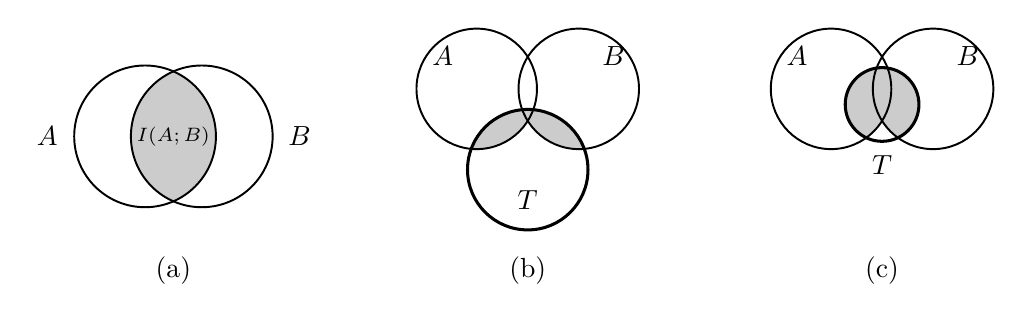
\begin{tikzpicture}[line width=0.7pt, scale=0.90,
		lens/.style={fill=black!20}]
		% ---- (a) I(A;B) ----
		\begin{scope}[yshift=-0.15cm]
			\begin{scope}
				\clip (-0.40,0) circle (1.00);
				\fill[lens] (0.40,0) circle (1.00);
			\end{scope}
			\draw (-0.40,0) circle (1.00);
			\draw (0.40,0) circle (1.00);
			\node at (-1.78,0) {\(A\)};
			\node at (1.78,0) {\(B\)};
			\node[font=\scriptsize] at (0,0) {\(I(A;B)\)};
			\node at (0,-1.90) {(a)};
		\end{scope}
		% ---- (b) complementary: A and B reach T in two different places ----
		\begin{scope}[xshift=5.0cm]
			\begin{scope}
				\clip (0,-0.62) circle (0.85);
				\fill[lens] (-0.72,0.52) circle (0.85);
				\fill[lens] (0.72,0.52) circle (0.85);
			\end{scope}
			\draw (-0.72,0.52) circle (0.85) node[above left=0.24cm] {\(A\)};
			\draw (0.72,0.52) circle (0.85) node[above right=0.24cm] {\(B\)};
			\draw[line width=1.1pt] (0,-0.62) circle (0.85);
			\node at (0,-1.05) {\(T\)};
			\node at (0,-2.05) {(b)};
		\end{scope}
		% ---- (c) redundant: same A and B, T moved onto their overlap ----
		\begin{scope}[xshift=10.0cm]
			\begin{scope}
				\clip (0,0.30) circle (0.52);
				\fill[lens] (-0.72,0.52) circle (0.85);
				\fill[lens] (0.72,0.52) circle (0.85);
			\end{scope}
			\draw (-0.72,0.52) circle (0.85) node[above left=0.24cm] {\(A\)};
			\draw (0.72,0.52) circle (0.85) node[above right=0.24cm] {\(B\)};
			\draw[line width=1.1pt] (0,0.30) circle (0.52);
			\node at (0,-0.55) {\(T\)};
			\node at (0,-2.05) {(c)};
		\end{scope}
	\end{tikzpicture}
	\caption[Mutual information and truth overlap]{%
		(a) Mutual information \(I(A;B)\), Eq.~\ref{eq:qgmiMIdef}, as the shared area
		of two variables in information space. (b) and (c): the observables \(A\) and
		\(B\) are drawn identically in the two panels, so their correlation
		\(I(A;B)\) is the same; only the truth bit \(T\) has moved. Shaded is the
		joint truth overlap \(I(T;A,B)\), the part of \(T\) reached by either
		observable. In (b) the two reach \(T\) in different places and the shaded
		region is much larger than the part either reaches alone, so combining them
		gains; in (c) they reach it in the same place, the shaded region is barely
		larger than either lobe, and combining them gains nothing. Correlation
		between observables and complementarity for discrimination are therefore
		separate questions. After Ref.~\cite{Larkoski_2014}.}
	\label{fig:qgmiVenn}
\end{figure}

The distinction the paper is built around is between \(I(A;B)\) and
\begin{equation}
	I(T;A,B) = H(T) + H(A,B) - H(T,A,B)
	\;\geq\; \max\left\{I(T;A),\,I(T;B)\right\} ,
	\label{eq:qgmiJoint}
\end{equation}
the truth overlap of the \emph{pair}. The first measures whether two observables are
correlated; the second measures whether their correlation, or lack of it, is of any
use. Figure~\ref{fig:qgmiVenn}(b) and (c) are drawn with identical \(I(A;B)\) and
identical individual truth overlaps and different \(I(T;A,B)\). This resolves a
standing puzzle in the substructure literature, where two variables are repeatedly
found to be weakly correlated and yet to gain nothing when combined: they are
uncorrelated in the bits that carry no flavour information and redundant in the bits
that do. The useful figure of merit is therefore the \emph{gain}
\begin{equation}
	\Delta I(T;A\to A,B) \equiv I(T;A,B) - \max\left\{I(T;A),I(T;B)\right\} ,
	\label{eq:qgmiGain}
\end{equation}
not the correlation coefficient.

\subsection{Casimir scaling, and why it caps the answer near a tenth of a bit}
\label{subsec:qgmiCasimir}

Call an observable \emph{Casimir scaling} if its cumulative distributions --- the
fraction of jets with the observable below \(\lambda\) --- take the form
\begin{equation}
	\Sigma_q(\lambda) = e^{-C_F\,r(\lambda)} ,
	\qquad
	\Sigma_g(\lambda) = e^{-C_A\,r(\lambda)}
	= \left[\Sigma_q(\lambda)\right]^{C_A/C_F} ,
	\label{eq:qgmiCasimir}
\end{equation}
for \emph{any} monotonic \(r\). The quark and gluon curves differ by a power, and by
nothing else: the observable has seen the jet's colour charge and no other property
of it. Equation~\ref{eq:qgmiCasimir} is the generic outcome of the cascade, because
Eq.~\ref{eq:qgmiLundPlane} puts \(\mathbf{Q}_i^2\) in front of the whole emission
density and nowhere else.

Cutting at \(\lambda<\lambda_{\rm cut}\) keeps a fraction \(x=\Sigma_q\) of quarks and
\(x^{C_A/C_F}\) of gluons, so the entire ROC curve is fixed,
\begin{equation}
	\varepsilon_g = \varepsilon_q^{\,C_A/C_F} = \varepsilon_q^{\,9/4} ,
	\label{eq:qgmiROC}
\end{equation}
independent of \(r\). The truth overlap is fixed with it, and the cleanest way to see
this is to note that Eq.~\ref{eq:qgmiMIdef} is invariant under any invertible change
of variable, so one may as well use \(\Sigma_q\) itself as the observable. Setting
\(\varrho\equiv C_A/C_F\) and \(w\equiv\Sigma_q(\lambda)\in[0,1]\), the quark
distribution of \(w\) is uniform by construction and the gluon distribution follows
from \(\Sigma_g=w^{\varrho}\),
\begin{equation}
	p_q(w) = 1 ,
	\qquad
	p_g(w) = \frac{d}{dw}w^\varrho = \varrho\,w^{\varrho-1} ,
	\label{eq:qgmiUniform}
\end{equation}
and every trace of the observable has disappeared. Substituting in
Eq.~\ref{eq:qgmiTruthOverlap},
\begin{equation}
	I(T;A) = \frac{1}{2}\int_0^1 dw\left[
	\log_2\frac{2}{1+\varrho w^{\varrho-1}}
	+ \varrho w^{\varrho-1}\log_2\frac{2\varrho w^{\varrho-1}}{1+\varrho w^{\varrho-1}}
	\right]
	\;\xrightarrow[\;\varrho=9/4\;]{}\;
	0.103 .
	\label{eq:qgmiBaseline}
\end{equation}
Every Casimir-scaling observable, whatever it measures and however well it is
measured, returns the same \(0.103\) of the one available bit. This is the number
against which everything else in this section is compared, and it is the quantitative
form of the remark closing Sec.~\ref{sec:coherentPartonBranching}: the separation is
statistical, the distributions overlap heavily, and the overlap is not an artifact of
any particular choice of observable.

The IRC safe angularities are Casimir scaling at leading logarithmic accuracy. An
emission carries \(\lambda^1_\beta\) above \(\lambda\) when \(u+\beta v<\ln(1/\lambda)\),
a triangle of area \(\ln^2(1/\lambda)/2\beta\) in the plane of
Eq.~\ref{eq:qgmiLundPlane}; vetoing every such emission, exactly as the Sudakov form
factor Eq.~\ref{eq:coherentSudakov} vetoes resolvable branchings, gives
\begin{equation}
	\Sigma_i(\lambda^1_\beta) = \exp\left[-\frac{\alpha_s}{\pi}
	\frac{\mathbf{Q}_i^2}{\beta}\ln^2\lambda^1_\beta\right] ,
	\label{eq:qgmiLLsudakov}
\end{equation}
which is Eq.~\ref{eq:qgmiCasimir} with \(r=(\alpha_s/\pi\beta)\ln^2\lambda\). So at
this order width, thrust and every angularity between them have \emph{identical}
discrimination power, \(0.103\) bits, and \(\beta\) has dropped out entirely. The
same is true, as Sec.~\ref{subsec:qgmiUnsafe} shows, of most of the IRC unsafe plane.
Casimir scaling is not a property of a few observables; it is what one gets by
default, and it explains the long-standing observation that wildly different
quark--gluon taggers perform almost identically.

\emph{Improving on \(0.103\) therefore requires resolving something in the jet other
than \(\mathbf{Q}_i^2\).}

\subsection{What breaks Casimir scaling}
\label{subsec:qgmiNLL}

Everything that distinguishes quark from gluon jets beyond the overall charge is
subleading in the logarithmic counting. Writing the cumulative distribution as
\begin{equation}
	\ln\Sigma(\lambda) = \underbrace{\alpha_s\ln^2\lambda}_{\rm LL}
	+ \underbrace{\alpha_s\ln\lambda}_{\rm NLL}
	+ \alpha_s + \mathcal{O}(\alpha_s^2) ,
	\label{eq:qgmiLogCounting}
\end{equation}
LL keeps the first term with \(\alpha_s\ln^2\lambda\sim1\), NLL adds the second.
Ref.~\cite{Larkoski_2014} evaluates Eq.~\ref{eq:qgmiTruthOverlap} on NLL
distributions of the form
\begin{equation}
	\Sigma_i(\lambda^1_\beta) =
	\frac{e^{-\gamma_E R_i^\prime}}{\Gamma(1+R_i^\prime)}\,
	e^{-R_i(\lambda^1_\beta)-\gamma_i T(\lambda^1_\beta)} ,
	\qquad
	R_i^\prime \equiv -\frac{dR_i}{d\ln\lambda^1_\beta} ,
	\label{eq:qgmiNLLcum}
\end{equation}
in which three distinct things spoil Eq.~\ref{eq:qgmiCasimir}, in increasing order of
physical interest.

\begin{enumerate}
	\item \textbf{The running coupling.} \(\alpha_s\) in Eq.~\ref{eq:qgmiLLsudakov} is
	really evaluated at the transverse momentum of each emission,
	\(\alpha_s(p_Tz\theta)\) --- Eq.~\ref{eq:runningCouplingLambda} with the scale
	fixed by Eq.~\ref{eq:tAndPt} --- so the radiator becomes a function of
	\(\lambda_\beta\equiv2\alpha_s\beta_0\ln\lambda^1_\beta\) rather than of
	\(\ln^2\lambda\). The exponent is still \(\propto\mathbf{Q}_i^2\), so this alone
	preserves Casimir scaling, but it sets the scale at which the other two act.

	\item \textbf{Multiple emissions.} The prefactor
	\(e^{-\gamma_ER^\prime}/\Gamma(1+R^\prime)\) corrects the LL assumption that a
	single emission dominates \(\lambda^1_\beta\); since
	\(R^\prime\propto\mathbf{Q}_i^2\) and \(\Gamma\) is not an exponential, this is a
	genuine, though mild, violation.

	\item \textbf{The hard-collinear splitting functions.} This is the physical one.
	\(\gamma_i\) in Eq.~\ref{eq:qgmiNLLcum} is the non-cusp anomalous dimension, which
	is nothing but the \(z\)-integral of the regularized splitting functions of
	Table~\ref{tab:splitfns} away from their soft poles,
	\begin{equation}
		\gamma_q = \frac{3}{4}C_F = 1 ,
		\qquad
		\gamma_g = \frac{11}{12}C_A - \frac{n_f}{6} = \frac{23}{12} ,
		\qquad
		\frac{\gamma_g}{\gamma_q} = \frac{23}{12} \neq \frac{9}{4} .
		\label{eq:qgmiNonCusp}
	\end{equation}
	A quark emits by \(\hat{P}_{qq}\) only; a gluon emits by \(\hat{P}_{gg}\) and
	splits by \(\hat{P}_{qg}\), and its \(n_f\) flavours of quark pair are a channel a
	quark jet does not have. In the soft limit \(z\to0\) all of these collapse to
	\(2\mathbf{Q}_i^2/z\) and only the charge survives, which is why LL sees only
	\(9/4\). At finite \(z\) they differ in \emph{shape}, and
	\(23/12\neq9/4\) is the first place the cascade remembers what opened the jet.
\end{enumerate}

The outcome is that \(I(T;\lambda^1_\beta)\) is no longer flat in \(\beta\): it rises
monotonically as \(\beta\) falls towards zero, reaching roughly \(0.11\)--\(0.13\) at
\(\beta\simeq0.5\) against the \(0.103\) LL baseline. Small \(\beta\) weights all
angles alike and so counts emissions rather than measuring their spread, moving the
observable towards multiplicity --- the best single discriminant in both parton
showers. In the plane of Eq.~\ref{eq:qgmiLundPlane} this is the statement that the
flavour information lives at large \(u\) and small \(v\), soft and wide-angle, which
is precisely the corner grooming removes; see Sec.~\ref{subsec:qgmiThesis}.

Two cautions come with this. The NLL result is a perturbative one and omits
non-perturbative power corrections, so it should not be trusted below
\(\beta\simeq0.5\). And when the same truth overlaps are extracted from
\textsc{Pythia}~8 and \textsc{Herwig}\texttt{++} the two disagree with each other and with NLL by amounts
comparable to the entire effect --- \textsc{Pythia}~8 systematically more optimistic, \textsc{Herwig}\texttt{++}
close to the LL baseline. The disagreement does \emph{not} appear when quark and
gluon distributions are compared individually; it appears only in their separation.
That is a warning about every Monte-Carlo-based estimate of tagging performance, and
the reason the paper's closing recommendation to the LHC experiments is for unfolded
angularity distributions over a range of \(\beta\) in purified samples.

\subsection{Charged-particle angularities: the weighted-energy function}
\label{subsec:qgmiUnsafe}

The measurement in Chapter~\ref{ch:angularities} restricts Eq.~\ref{eq:qgmiAngularity}
to tracks, which as noted there costs IRC safety. Ref.~\cite{Larkoski_2014} handles
the whole \(\kappa\neq1\) plane with the same device that makes track-based
observables calculable: factor the non-perturbative step into an object with a
perturbative evolution, exactly as Sec.~\ref{sec:partonShower} factors hadronization
out of the cascade.

The object is the \emph{weighted-energy function} \(F^i_\kappa(x,\mu)\), the
probability that a parton of flavour \(i\) fragments into a set of hadrons with
\(\sum_h z_h^\kappa = x\), normalized to \(\int_0^\infty dx\,F^i_\kappa(x,\mu)=1\).
It is the \(\kappa\)-weighted sibling of the fragmentation function \(D^h_i(x,t)\):
where \(D\) tracks one hadron's share of the parton's energy, \(F\) tracks the whole
final state's contribution to \(\lambda^\kappa_0\) in one number. For \(\kappa=1\)
restricted to charged particles it is the track function, and weighted by charge it
is the jet charge distribution. Being non-perturbative it must be measured, but it
evolves perturbatively with the splitting functions already in
Table~\ref{tab:splitfns},
\begin{equation}
	\mu\frac{\partial}{\partial\mu}F^i_\kappa(x,\mu)
	= \frac{1}{2}\sum_{j,k}\int dz\,dx_1\,dx_2\,
	\frac{\alpha_s}{\pi}\hat{P}_{i\to jk}(z)\,
	F^j_\kappa(x_1,\mu)F^k_\kappa(x_2,\mu)\,
	\delta\!\left(x - (1-z)^\kappa x_1 - z^\kappa x_2\right) ,
	\label{eq:qgmiFRGE}
\end{equation}
with the jet's own scale \(\mu=p_{\rm T}R\). Equation~\ref{eq:qgmiFRGE} is
Sec.~\ref{subsec:dglap}'s DGLAP equation with the convolution moved from the momentum
fraction into the observable: both daughters are kept, each carrying its own \(F\),
and the \(\delta\) function adds their contributions with the \(\kappa\)-weights the
observable demands. It is, in other words, the parton shower, written for this
observable. Measure \(F^i_\kappa\) once and Eq.~\ref{eq:qgmiFRGE} transports it to any
other jet \(p_{\rm T}\) or radius; the paper checks this against both showers for
\(p_T^D\).

The remarkable result is what happens for \(\beta>0\). Repeating the veto argument of
Eq.~\ref{eq:qgmiLLsudakov} with the emission now fragmenting, the radiator is
\begin{equation}
	R_i(\lambda^\kappa_\beta) = \int_0^1\frac{d\theta}{\theta}\int_0^1 dz\,
	\frac{\alpha_s(p_{\rm T}z\theta)}{\pi}\hat{P}_{gi}(z)
	\int_0^\infty dx\,F^g_\kappa(x,\mu)\,
	\Theta\!\left(x z^\kappa\theta^\beta - \lambda^\kappa_\beta\right) ,
	\label{eq:qgmiUnsafeRadiator}
\end{equation}
and the \(\Theta\) function can be rewritten
\(\Theta(z\theta^{\beta/\kappa}-(\lambda^\kappa_\beta/x)^{1/\kappa})\), which is the
condition for the \emph{IRC safe} angularity of exponent \(\beta/\kappa\). All that
survives of \(F\) at NLL is its first logarithmic moment,
\begin{equation}
	f^{g,n}_\kappa \equiv \int_0^\infty dx\,F^g_\kappa(x,\mu)\ln^n x ,
	\qquad
	f^{g,1}_\kappa \approx 3(1-\kappa) ,
	\label{eq:qgmiLogMoment}
\end{equation}
entering as a rescaling \(x\to\exp(f^{g,1}_\kappa)\), so that the entire IRC unsafe
problem collapses onto the IRC safe one:
\begin{equation}
	R_i^{\rm NLL}(\lambda^\kappa_\beta)
	= \hat{R}_i^{\rm NLL}\!\left(
	\lambda^1_{\beta/\kappa} =
	\left[\frac{\lambda^\kappa_\beta}{\exp f^{g,1}_\kappa}\right]^{1/\kappa}\right) .
	\label{eq:qgmiCollapse}
\end{equation}
A collinear-unsafe observable is computed from a collinear-safe one, at a shifted
angular exponent and with the non-perturbative physics reduced to a single number per
\(\kappa\) --- a number, moreover, that \textsc{Pythia}~8 and \textsc{Herwig}\texttt{++} agree on, unlike
almost everything else in this section. At LL the moments drop out and
\begin{equation}
	R_i^{\rm LL}(\lambda^\kappa_\beta) = \frac{\alpha_s}{\pi}
	\frac{\mathbf{Q}_i^2}{\beta\kappa}\ln^2\lambda^\kappa_\beta ,
	\label{eq:qgmiUnsafeLL}
\end{equation}
Casimir scaling again, and the \(0.103\) of Eq.~\ref{eq:qgmiBaseline} again, now over
most of the \((\beta,\kappa)\) plane rather than just the line \(\kappa=1\).

Equation~\ref{eq:qgmiUnsafeLL} also delimits its own validity. The \(1/\beta\kappa\)
prefactor requires \(\beta\kappa\gtrsim0.5\) for the logarithms to be resummable at
all; and the log moment must stay below the typical \(\ln\lambda^\kappa_\beta\),
which with the peak at \(\ln^2\lambda^\kappa_\beta=\beta\kappa/2\alpha_s\mathbf{Q}_i^2\)
and Eq.~\ref{eq:qgmiLogMoment} gives
\begin{equation}
	\frac{\beta\kappa}{(1-\kappa)^2} > 18\alpha_s\mathbf{Q}_i^2 \simeq 6
	\quad(\text{gluons}) ,
	\label{eq:qgmiBarrier}
\end{equation}
the contour drawn in Fig.~\ref{fig:qgmiLambdaSpace}. Outside it the whole function
\(F^g_\kappa(x,\mu)\) is needed, not a moment of it. The honest summary is that the
two regions where the parton showers show the most interesting structure --- near
multiplicity and near \(p_T^D\) --- are the two the calculation cannot reach.

\subsection{The \(\beta=0\) axis: multiplicity and \(p_T^D\)}
\label{subsec:qgmiBetaZero}

On the axis \(\beta=0\) there is no angular weight at all, \(\lambda^\kappa_0=\sum_c z_c^\kappa\),
and at lowest order the distribution \emph{is} the weighted-energy function,
\(\sigma_i^{-1}d\sigma_i/d\lambda^\kappa_0 = F^i_\kappa(\lambda^\kappa_0,\mu)\).
Nothing is predicted; but Eq.~\ref{eq:qgmiFRGE} still evolves it, so the jet
\(p_{\rm T}\) and \(R\) dependence is calculable even when the distribution is not.
Note \(\lambda^1_0=\sum_cz_c=1\) identically, so the \(\kappa\to1\) limit must be
taken as \(\lambda^\kappa_0\to1+(\kappa-1)\sum_cz_c\ln z_c\), i.e.\ the observable
there is \(\sum_c z_c\ln z_c\).

Two corners of this axis are the standard taggers. \(\lambda^0_0\), constituent
multiplicity, is the best single discriminant in both showers and lies entirely
outside the formalism: at \(\kappa=0\) the observable is infrared unsafe as well as
collinear unsafe, and counting soft emissions is governed by the
double-logarithmic growth of \(\langle n\rangle\) rather than by any Sudakov veto.
\(\lambda^2_0 = p_T^D\) is calculable through its evolution and is the observable
that adds most to multiplicity in both showers. That the two most useful
discriminants in practice sit on the one line the theory handles worst is the central
tension of the paper, and its suggested way out --- grooming the jet first, so that
the soft radiation responsible for the infrared unsafety is removed before the
observable is formed --- is the subject of Sec.~\ref{subsec:qgmiThesis}.

\subsection{Two angularities at once}
\label{subsec:qgmiPairs}

For two IRC safe angularities with \(\alpha>\beta\), the LL double cumulative follows
from the same triangle construction applied twice,
\begin{equation}
	\Sigma_i(\lambda^1_\alpha,\lambda^1_\beta) = \exp\left[-\frac{\alpha_s}{\pi}
	\mathbf{Q}_i^2\left(\frac{\ln^2\lambda^1_\beta}{\beta}
	+ \frac{\ln^2(\lambda^1_\alpha/\lambda^1_\beta)}{\alpha-\beta}\right)\right] ,
	\label{eq:qgmiDoubleLL}
\end{equation}
on the phase space \(\lambda^1_\beta>\lambda^1_\alpha\) and
\((\lambda^1_\alpha)^\beta>(\lambda^1_\beta)^\alpha\), which is the statement that the
two observables are two different projections of the same single emission and so
cannot take independent values. Equation~\ref{eq:qgmiDoubleLL} is still
\(\propto\mathbf{Q}_i^2\) in the exponent, but it is a Casimir-scaling exponent of two
variables, and the universality argument of Eq.~\ref{eq:qgmiUniform} --- which relied
on mapping a single observable onto a uniform variable --- no longer applies. This is
the first place a gain over \(0.103\) appears without going to NLL: for
\((\lambda^1_2,\lambda^1_{0.5})\) the joint truth overlap exceeds \(0.12\) already at
LL. Measuring the \emph{same} emission two different ways recovers information about
its \(z\) and \(\theta\) separately, which a single projection has integrated away.
Unsurprisingly, the pairs with the largest gain \(\Delta I\) are broadly those with
the smallest \(I(\lambda^1_\alpha;\lambda^1_\beta)\), though with enough scatter that
the correlation is not a reliable proxy.

The most useful result in this part of the paper is a negative one, and it is worth
stating plainly because it bears directly on how a measurement should be compared to
theory. Across the four methods --- LL, NLL, \textsc{Pythia}~8, \textsc{Herwig}\texttt{++} --- the
\emph{correlation} \(I(\lambda^1_\alpha;\lambda^1_\beta)\), computed on quark and
gluon samples separately, agrees closely. The \emph{truth overlap}
\(I(T;\lambda^1_\alpha,\lambda^1_\beta)\) does not: \textsc{Pythia}~8 exceeds the NLL
calculation, which exceeds \textsc{Herwig}\texttt{++}, which sits near the LL baseline, and the four
even disagree about \emph{which} pairs are worth combining. The structure of a jet is
well under control; the difference between two flavours of jet is not. Double
differential distributions of \(\lambda^1_\alpha\) and \(\lambda^1_\beta\) are
therefore the paper's second recommendation to experiment.

\subsection{Consequences for the measurement of Chapter~\ref{ch:angularities}}
\label{subsec:qgmiThesis}

Collecting what bears on this thesis:

\begin{itemize}
	\item \textbf{The quark and gluon fractions must be fixed before any
	medium effect is read off.} Equations~\ref{eq:qgmiROC} and \ref{eq:qgmiBaseline}
	say that \emph{every} angularity separates the two species, by an amount that is
	the same for all of them at leading order and does not go away. A change in
	\(\langle\lambda^\kappa_\beta\rangle\) between \pp and \AuAu is a change in the
	flavour admixture until shown otherwise, and the size of that systematic is set by
	Eq.~\ref{eq:qgmiROC}, which is calculable.

	\item \textbf{Charged-only angularities are IRC unsafe, and this is the
	framework that handles them.} The weighted-energy function
	\(F^i_\kappa\) of Eq.~\ref{eq:qgmiFRGE} and its collapse onto an IRC safe
	angularity of exponent \(\beta/\kappa\), Eq.~\ref{eq:qgmiCollapse}, is the
	quantitative version of the remark following Eq.~\ref{eq:LambdaKappaBeta} that
	track-based angularities require non-perturbative fragmentation input. The input
	is one number, \(f^{g,1}_\kappa\), and it is the one quantity in this section that
	the event generators agree on.

	\item \textbf{Grooming is the recommended fix, and the decomposition in
	Chapter~\ref{ch:angularities} is already in the right form.} The paper's own
	proposal for escaping both the non-global logarithms and the infrared unsafety at
	\(\kappa=0\) is to compute angularities on SoftDrop-groomed jets, where the
	cumulative distribution again exhibits Casimir scaling at LL. The split
	\(\lambda^\kappa_\beta = \lambda^\kappa_{\beta,\mathrm{pQCD}}
	+ \Delta\lambda^\kappa_\beta\) of Chapter~\ref{ch:angularities} is exactly that
	separation --- and Sec.~\ref{subsec:qgmiNLL} adds the caveat that grooming removes
	the soft wide-angle region where the non-Casimir, flavour-sensitive information
	sits. Groomed angularities are more calculable and, for that same reason, worse
	discriminants. Fig.~\ref{fig:GroomingAndRg} is a picture of what is being given up.

	\item \textbf{Use a recoil-free axis if the analytic results are to be
	compared quantitatively.} See Sec.~\ref{subsec:qgmiFamily}. With the standard jet
	axis the \(\beta\lesssim1\) results above do not apply as written.

	\item \textbf{Report distributions, not just performance.} Both of the paper's
	recommendations to experiment --- unfolded \(\lambda^1_\beta\) over a range of
	\(\beta\), and double differential distributions of angularity pairs --- describe
	the \pp measurement of Chapter~\ref{ch:angularities}. The disagreement between
	\textsc{Pythia}~8 and \textsc{Herwig}\texttt{++} in Sec.~\ref{subsec:qgmiNLL} is large, unexplained, and
	invisible in single-flavour observables, which makes an unfolded measurement the
	only way to settle it.
\end{itemize}

%% =====================================================================
%  jetportrait.tex -- Secs. 1.4.5-1.4.7.
%
%  Follows Ellis, Stirling & Webber (ESW), "QCD and Collider Physics",
%  Ch. 6 "Jet properties beyond fixed order" -- the chapter after the
%  one Secs. 1.4.1-1.4.4 are built on -- section for section:
%      1.4.5 Jet fragmentation  <-> ESW 6.1
%      1.4.6 Jet substructure    <-> ESW 6.4 + 6.5, extended with
%              Dokshitzer-Khoze-Mueller-Troyan (BPQCD) Sec. 9.2.
%  Supersedes qgjets.tex.
%
%  BIBTEX NEEDED in thesis.bib -- keys below are undefined until pasted.
%  ESW Ch. 5 (...1996d) is what Secs. 1.4.1-1.4.4 follow and is not
%  cited anywhere yet; it is offered here, not cited by this file.
%
%  @incollection{Ellis_Stirling_Webber_1996d,
%    author={Ellis, R. K. and Stirling, W. J. and Webber, B. R.},
%    title={Parton branching and jet simulation},
%    booktitle={QCD and Collider Physics},
%    series={Cambridge Monographs on Particle Physics, Nuclear Physics
%            and Cosmology},
%    publisher={Cambridge University Press}, address={Cambridge},
%    year={1996}, pages={157--192}}
%
%  @incollection{Ellis_Stirling_Webber_1996e,
%    author={Ellis, R. K. and Stirling, W. J. and Webber, B. R.},
%    title={Jet properties beyond fixed order},
%    booktitle={QCD and Collider Physics},
%    series={Cambridge Monographs on Particle Physics, Nuclear Physics
%            and Cosmology},
%    publisher={Cambridge University Press}, address={Cambridge},
%    year={1996}, pages={193--236}}
%
%  @book{Dokshitzer_Khoze_Mueller_Troyan_1991,
%    author={Dokshitzer, Yu. L. and Khoze, V. A. and Mueller, A. H.
%            and Troyan, S. I.},
%    title={Basics of Perturbative QCD},
%    publisher={Editions Fronti\`{e}res}, address={Gif-sur-Yvette},
%    year={1991}}
%
%  @article{Azimov_Dokshitzer_Khoze_Troyan_1985,
%    author={Azimov, Ya. I. and Dokshitzer, Yu. L. and Khoze, V. A.
%            and Troyan, S. I.},
%    title={Similarity of Parton and Hadron Spectra in {QCD} Jets},
%    journal={Z. Phys. C}, volume={27}, number={1}, pages={65--72},
%    year={1985}}
%
%  NOTATION -- ESW's throughout, so this reads on from 1.4.1-1.4.4:
%   D^h_i(x,t): subscript = initiating parton, superscript = observed.
%   The z^2 in eq:timelikeDglap is ESW (6.25) and is your own
%     eq:orderingCutoff; without it the small-x behaviour is wrong.
%   xi = ln(1/x), ESW (6.39).  (Hence no integrated-coupling xi; the one
%     place it is needed, eq:valenceSpectrum, uses a local w.)
%   ESW's b, from beta(a_s) = -b a_s^2, IS your beta_0 of eq:RGEquation,
%     and their a_s = 1/(b ln(s/L^2)) is your eq:runningCouplingLambda,
%     so eq:dlaMultiplicity is ESW (6.37) verbatim in your symbols.
%
%  ON beta_0 -- flagged, not touched.  Derivations are symbolic in
%  alpha_s = 1/(beta_0 ln(t/Lambda^2)) and hold whatever beta_0 is.  The
%  numbers (50/81, 2.4, 1/4) need 4 pi beta_0 = 11 - 2N_f/3, which is
%  also what ESW's b equals; intro.tex:178 carries an extra 4 pi
%  relative to the RGE at intro.tex:172 (beta_1 with (4pi)^4 is right).
%  BPQCD's b = 4 pi beta_0, hence the exponent of
%  eq:colorCurrentEvolution.  BPQCD (9.12) prints gamma there but their
%  (9.15) uses 50/81 = (50/9)/9, so gamma/(4 pi beta_0) is meant.
%  Signs in eq:multCollimationEq: <Q^2>_q/C_F = 1.8 - 0.8r and
%  <Q^2>_g/C_A = 0.8 + 0.2r; BPQCD (9.15) quotes both positive.
% =====================================================================

\subsection{Jet fragmentation}
\label{subsec:fragmentation}

A jet of energy \(E\) and opening angle \(\theta\) enters the cascade of
Sec.~\ref{sec:coherentPartonBranching} at its \emph{hardness}
\(\tilde{t}=E^2(1-\cos\theta)\simeq(E\theta)^2/2\); a cone of half-angle
\(\theta^\prime<\theta\) about its axis sits at \(\tilde{t}^\prime<\tilde{t}\) on the
same ladder, so narrowing the aperture and stopping the cascade early are one
operation. The \emph{fragmentation function} \(D^h_i(x,\tilde{t})\), the inclusive
probability of a hadron \(h\) with \(x=E_h/E_i\) in a jet opened by a parton \(i\),
evolves with the regularized Altarelli--Parisi kernels \(P_{ji}(z)\) --- the
\(\hat{P}_{ji}\) of Table~\ref{tab:splitfns} with their plus-prescription and
\(\delta(1-z)\) terms restored --- as
\begin{equation}
	\tilde{t}\frac{\partial}{\partial\tilde{t}}D^h_i(x,\tilde{t})
	= \sum_j\int_x^1\frac{dz}{z}\frac{\alpha_s}{2\pi}
	P_{ji}(z)\,D^h_j\!\left(\frac{x}{z}, z^2\tilde{t}\right) ,
	\label{eq:timelikeDglap}
\end{equation}
the \(z^2\) being Eq.~\ref{eq:orderingCutoff} and the only place coherence enters;
stopping at an intermediate scale gives the parton-level
\(D^j_i(x;\tilde{t},\tilde{t}^\prime)\). The first moment
\(\langle n_h\rangle_i=\int_0^1dx\,D^h_i\) diverges at lowest order, the moments of
\(P_{ji}\) being dominated by \(P_{gi}\to2\mathbf{Q}_i^2/z\); the \(z^2\)
regulates it, \(D\propto\tilde{t}^{\,\gamma}\) requiring
\(\gamma=\frac{\alpha_s}{2\pi}\int_0^1dz\,z^{\,j-1+2\gamma}P(z)\), so that
\begin{align}
	\gamma_{gg}(j,\alpha_s) &= \frac{1}{4}\left[
	\sqrt{(j-1)^2 + \frac{8C_A\alpha_s}{\pi}} - (j-1)\right]
	\;\xrightarrow[\;j\to1\;]{}\;
	\sqrt{\frac{C_A\alpha_s}{2\pi}} , \notag\\
	\langle n(\tilde{t})\rangle &\propto
	\exp\left[\int^{\tilde{t}}\gamma_{gg}(1,\alpha_s)
	\frac{d\tilde{t}^\prime}{\tilde{t}^\prime}\right]
	\propto
	\exp\left[\sqrt{\frac{2C_A}{\pi\beta_0}\ln\frac{\tilde{t}}{\Lambda^2}}\;\right] ,
	\label{eq:dlaMultiplicity}
\end{align}
a square root of \(\alpha_s\): the soft singularities are resummed, and
\(\langle n\rangle\) outgrows any power of \(\ln\tilde{t}\) while staying below any
power of \(\tilde{t}\). Keeping only these double logarithms is the
\emph{double-logarithmic approximation} (DLA), adding the next-to-leading ones the
\emph{modified leading-logarithmic approximation} (MLLA). Away from \(j=1\) the same
\(\gamma_{gg}\) gives a Gaussian in \(\xi\equiv\ln(1/x)\),
\begin{equation}
	x D^h_i \propto \exp\left[-\frac{(\xi-\xi_p)^2}{2\sigma^2}\right],
	\quad
	\xi_p = \frac{1}{4\beta_0\alpha_s(\tilde{t})}
	\simeq \frac{1}{4}\ln\frac{\tilde{t}}{\Lambda^2},
	\quad
	\sigma \propto \left[\ln\frac{\tilde{t}}{\Lambda^2}\right]^{3/4} ,
	\label{eq:humpBacked}
\end{equation}
the \emph{hump-backed plateau}~\cite{Azimov_Dokshitzer_Khoze_Troyan_1985}. A merely
kinematic cut-off at \(x\propto m/\sqrt{\tilde{t}}\) would put the peak at
\(\tfrac12\ln(\tilde{t}/\Lambda^2)\), twice the observed energy dependence: the soft
suppression is coherence.

\subsection{Jet substructure}
\label{subsec:substructure}

Every emission rate above is proportional to the emitter's squared colour charge, and
Eq.~\ref{eq:dlaMultiplicity} carries \(C_A\) whatever opened the jet, the cascade
being gluon-dominated after the first branching, so
\begin{equation}
	\frac{\mathbf{Q}_g^2}{\mathbf{Q}_q^2} = \frac{C_A}{C_F}
	= \frac{2N_c^2}{N_c^2-1} = \frac{9}{4} ,
	\qquad
	\langle n\rangle_i = \frac{\mathbf{Q}_i^2}{C_A}\langle n\rangle_g
	\;\Longrightarrow\;
	\frac{\langle n\rangle_g}{\langle n\rangle_q}
	\;\xrightarrow[\;\tilde{t}\to\infty\;]{}\;\frac{C_A}{C_F} .
	\label{eq:casimirRatio}
\end{equation}
The second moment is reduced likewise, widening a gluon jet's multiplicity
distribution by \(\sqrt{C_A/C_F}\), while in the spectrum the peak \(\xi_p\) is common
to both and only its height differs, as \(C_F:C_A\). For the angular size the
Sterman--Weinberg criterion, all but a fraction \(\epsilon\) of the energy inside a
half-angle \(\delta\), gives at fixed \(f_2,\epsilon\)
\begin{align}
	f_2 &= 1 - \frac{4\alpha_s\mathbf{Q}_i^2}{\pi}
	\ln\frac{1}{\epsilon}\ln\frac{1}{\delta} , \notag\\
	\delta_q &\sim \exp\left[\frac{\pi(1-f_2)}
	{4C_F\alpha_s(\tilde{t})\ln\epsilon}\right] ,
	\qquad
	\delta_g \sim \delta_q^{\,C_F/C_A} = \delta_q^{\,4/9} ,
	\label{eq:swWidth}
\end{align}
the charge in the denominator leaving the gluon jet the wider. Both ratios are
asymptotic: energy conservation and MLLA corrections bring the multiplicity ratio to
\(\simeq1.5\) at present energies.

Energy and multiplicity are not collimated alike. A cone \(\theta^\prime\) intercepts
the cascade at \(\tilde{t}^\prime\) (Eq.~\ref{eq:angularOrdering}), so the energy it
holds follows \(\sum_jD^j_i(z;\tilde{t},\tilde{t}^\prime)\); at \(z\to1\) the valence
term dominates and the \(z\to1\) singularity of \(P_{ii}\), exponentiated as in
Sec.~\ref{subsec:dglap}, gives \(D^i_i\propto(1-z)^{-1+4\mathbf{Q}_i^2w}\),
\(w=\int_{\tilde{t}^\prime}^{\tilde{t}}
(d\tilde{t}^{\prime\prime}/2\tilde{t}^{\prime\prime})(\alpha_s/2\pi)\), which falls at
both ends and peaks at
\begin{equation}
	\frac{\theta_z}{\theta} =
	\left(\frac{\sqrt{\tilde{t}}}{\Lambda}\right)^{-\gamma_E(z)},
	\qquad
	\begin{array}{r|cc}
		z & \gamma_E^{\,q}(z) & \gamma_E^{\,g}(z) \\ \hline
		0.9 & 0.55 & 0.30 \\
		0.5 & 0.83 & 0.54
	\end{array}
	\label{eq:energyCollimation}
\end{equation}
--- a power of the hardness, faster for quark jets, as in Eq.~\ref{eq:swWidth}. The
particles in that cone instead correlate the flux with one particle in it: convolving
\(D^j_i(z;\tilde{t},z^2\tilde{t}^\prime)\) with \(D^h_j(x/z,z^2\tilde{t}^\prime)\) at
\(x\ll1\), where Eq.~\ref{eq:humpBacked} is insensitive to the energy balance, gives
\(\langle n_h\rangle_i=(\langle\mathbf{Q}^2\rangle_i/C_A)\langle n_h\rangle_g\) with
\(\langle\mathbf{Q}^2\rangle_i=\langle z_g\rangle_iC_A+\langle z_q\rangle_iC_F\), the
\emph{average colour current} of the partons caught. Inside a cone every jet is a
gluon jet, and \(\langle\mathbf{Q}^2\rangle_{q,g}\to2.4\) as \(\theta^\prime\to0\), so
the \(9/4\) of Eq.~\ref{eq:casimirRatio} tends to \(1\) for a narrow cone at any
energy. Repeating for particles leaves a colour ratio between \(1\) and
\(\simeq1.8\), so Eq.~\ref{eq:dlaMultiplicity} alone fixes
\begin{equation}
	\theta_\delta \sim \theta\,
	\langle n(\tilde{t})\rangle^{-(\pi\beta_0/2C_A)\ln(1/\delta)} ,
	\qquad
	\frac{\pi\beta_0}{2C_A}\ln 2 \simeq 0.26 \simeq \frac{1}{4} .
	\label{eq:multCollimation}
\end{equation}
\(\langle n\rangle\) growing only as the exponential of a square root,
\(\theta_\delta\) falls slower than any power of the hardness where \(\theta_z\) falls
as a power (Fig.~\ref{fig:collimationCones}): a narrow core of energy in a broad halo
of particles, separating as the jet hardens.

\begin{figure}[htbp]
	\centering
	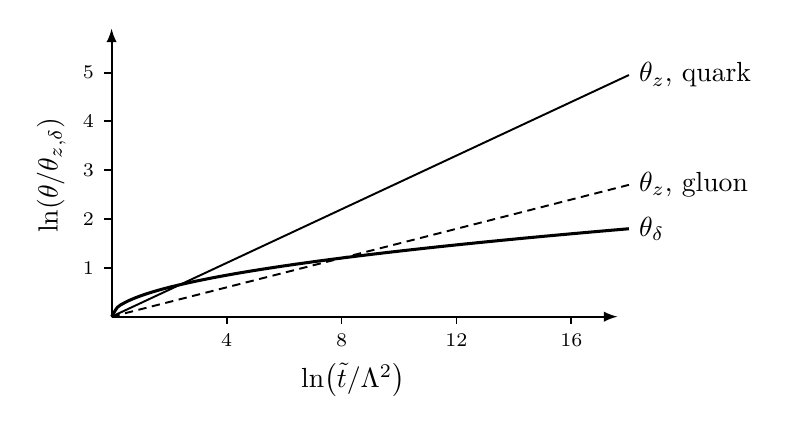
\begin{tikzpicture}[x=0.365cm, y=0.62cm, line width=0.7pt]
		\draw[->] (0,0) -- (17.6,0);
		\draw[->] (0,0) -- (0,5.9);
		\foreach \i in {4,8,12,16} {
			\draw (\i,0) -- (\i,-0.14) node[below] {\scriptsize\(\i\)};
		}
		\foreach \j in {1,2,3,4,5} {
			\draw (0,\j) -- (-0.26,\j) node[left] {\scriptsize\(\j\)};
		}
		\node[below] at (8.4,-0.75) {\(\ln(\tilde{t}/\Lambda^2)\)};
		\node[rotate=90] at (-2.1,2.9) {\(\ln(\theta/\theta_{z,\delta})\)};
		\draw[domain=0:18, samples=2] plot (\x, {0.275*\x});
		\draw[domain=0:18, samples=2, densely dashed] plot (\x, {0.150*\x});
		\draw[domain=0:18, samples=90, smooth, line width=1.1pt]
		plot (\x, {0.4245*sqrt(\x)});
		\node[right] at (18,4.95) {\(\theta_z\), quark};
		\node[right] at (18,2.70) {\(\theta_z\), gluon};
		\node[right] at (18,1.80) {\(\theta_\delta\)};
	\end{tikzpicture}
	\caption[Collimation of the energy and multiplicity flows of a jet]{%
		Collimation of the energy and of the multiplicity flow of a jet against its
		hardness, for \(z=0.9\), \(\delta=\tfrac12\), \(N_f=3\). The energy cone
		\(\theta_z\) of Eq.~\ref{eq:energyCollimation} closes linearly in
		\(\ln(\tilde{t}/\Lambda^2)\) and faster for quark jets; the multiplicity cone
		\(\theta_\delta\) of Eq.~\ref{eq:multCollimation} only as its square root.}
	\label{fig:collimationCones}
\end{figure}


The angularities of Chapter~\ref{ch:angularities} replace the cone by a weight, and
the same cascade fixes their distributions:
\begin{align}
	\lambda_\beta^\kappa &= \sum_{c\,\in J} z_c^\kappa
	\left(\frac{\Delta R_c}{R}\right)^{\beta} ,
	\qquad
	z_c = p_{\mathrm{T},c}\Big/\!\!\sum_{c^\prime\in J}p_{\mathrm{T},c^\prime} ,
	\notag\\
	dn &= \frac{2\alpha_s\mathbf{Q}_i^2}{\pi}\frac{dz}{z}\frac{d\theta}{\theta}
	= \frac{2\alpha_s\mathbf{Q}_i^2}{\pi}\,du\,dv ,
	\qquad
	u = \ln\frac{1}{z} , \qquad v = \ln\frac{R}{\theta} ,
	\label{eq:angularityDef}
\end{align}
the density being the single-emitter antenna pattern of
Eq.~\ref{eq:antennaSplitXSec} with \(\zeta\simeq\theta^2/2\), uniform on the quadrant,
each emission contributing \(z^\kappa(\theta/R)^\beta\) to the sum, which at this
accuracy is dominated by one of them. Let \(\Sigma_i(\lambda)\) be the fraction of
jets whose angularity falls below a value \(\lambda\). At \(\kappa=1\) an emission
carries \(\lambda^1_\beta\) above \(\lambda\) when \(u+\beta v<\ln(1/\lambda)\), a
triangle of area \(\ln^2(1/\lambda)/2\beta\), and vetoing every such emission gives
\begin{equation}
	\Sigma_i(\lambda) = \exp\left[-\frac{\alpha_s\mathbf{Q}_i^2}{\pi\beta}
	\ln^2\frac{1}{\lambda}\right] ,
	\qquad
	\Sigma_g(\lambda) = \left[\Sigma_q(\lambda)\right]^{C_A/C_F} ,
	\label{eq:angularitySudakov}
\end{equation}
a Sudakov form factor vetoing an observable rather than a cone, and at \(\beta=1\) the
double-logarithmic thrust distribution~\cite{Ellis_Stirling_Webber_1996e}. Equations~\ref{eq:swWidth} and
\ref{eq:angularitySudakov} invert one another. At \(\kappa=0\) the vetoed region is
instead the strip \(v<\ln(1/\lambda)/\beta\), unbounded in \(u\): nothing
exponentiates and \(\lambda^0_\beta\) counts emissions, governed by
Eq.~\ref{eq:dlaMultiplicity}. So \(\lambda^1_1\) is the jet width and measures
\(\theta_z\), \(\lambda^0_0\) the jet multiplicity and \(\theta_\delta\), and
\((\kappa,\beta)\) carries one into the other --- with the quark--gluon memory at
large \(u\), small \(v\), exactly where grooming cuts, so the quark and gluon
fractions of a sample must be fixed before a change in its angular structure is read
as a medium effect.








%===========================================================================================



\chapter{Solenoidal Tracker At Relativistic Heavy Ion Collider}
\label{ch:STAR}

\section{Relativistic Heavy-Ion Collider (RHIC)}
\label{sec:RHIC}

The Relativistic Heavy Ion Collider (RHIC), at Brookhaven National Laboratory (BNL), was the only collider with dedicated running for heavy ion research (the CERN Large Hadron Collider runs heavy ions for only about one month per year), and the only polarized proton collider ever built. Two concentric accelerator rings 2.4 miles in circumference containing a total of 1,740 superconducting magnets afforded RHIC the capability to independently accelerate and collide ion beam species from $\rm ^1_1H (p)$ to  $\rm ^{238}_{92}U$ at energies between 3.85 GeV and 254.9 GeV per nucleon and different spin polarizations for protons (\(p\)), as shown in Fig.~\ref{fig:RHICSpecies}. These capabilities made RHIC the most flexible and capable collider in the world for transformative studies of extreme states of nuclear matter and the origin of the proton spin.
\begin{figure}
	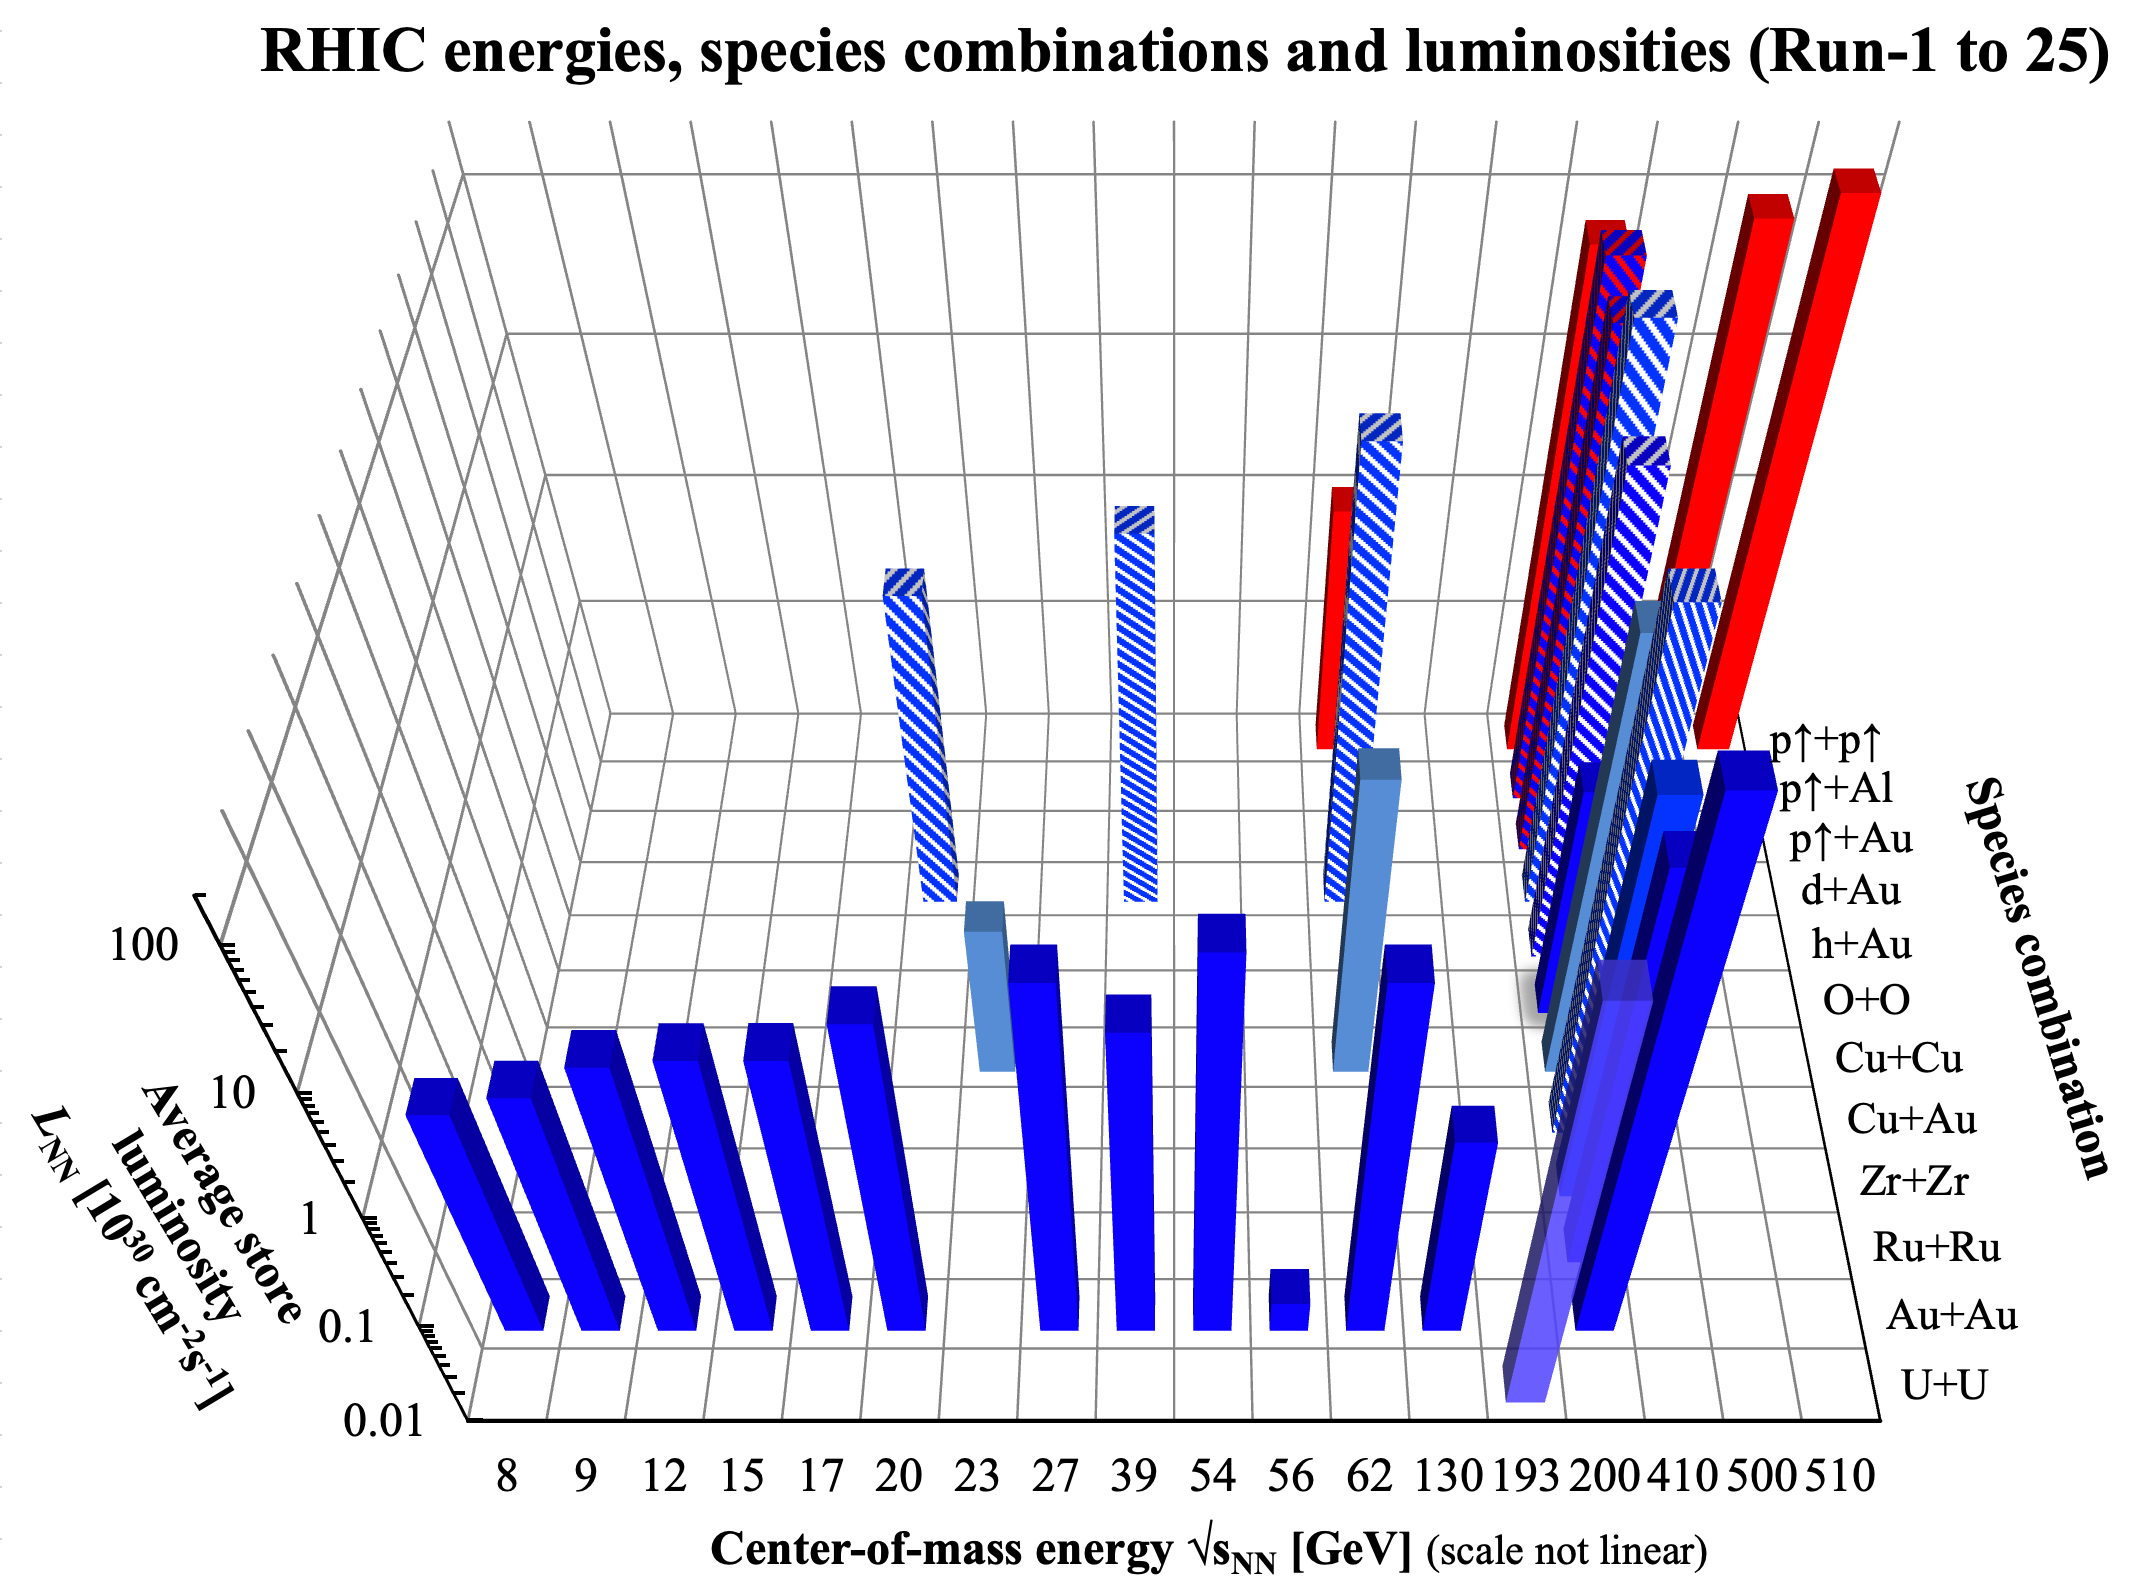
\includegraphics[width=\linewidth]{figures/RhicSpecies.png}
	\caption[RHIC energies, collision species and luminosities from 2000 to 2025]{Summary of RHIC energies, species combinations, and average store luminosities for Run~1 (2000) to Run~25 (2025)~\cite{RHICRunSummary}.}
	\label{fig:RHICSpecies}
\end{figure}

On February 6th 2026 RHIC ended operations with collisions of $\rm ^{16}_{8}O$ nuclei at \(\sqrt{s_\mathrm{NN}} = 200\)~GeV recorded by the \emph{Solenoidal Tracker At RHIC (STAR)} and \emph{sPHENIX} detectors. Over its 25 years of active existence, it performed \(\sim 300\)~trillion collisions of 49 unique pairs of nuclei, collected \(\sim 450\)~petabytes of data, whose analysis has led to over 650 publications. Event displays of some of the last collisions, recorded by both detectors, are shown in Fig.~\ref{fig:Final}. Eventually, one of RHIC’s ion storage rings will be removed and replaced with a new ring for storing accelerated electrons inside the existing accelerator tunnel, and the other major components of the RHIC accelerator complex will live on as parts of the upcoming Electron-Ion Collider (EIC)~\cite{AbdulKhalek:2021gbh}.
\begin{figure}
	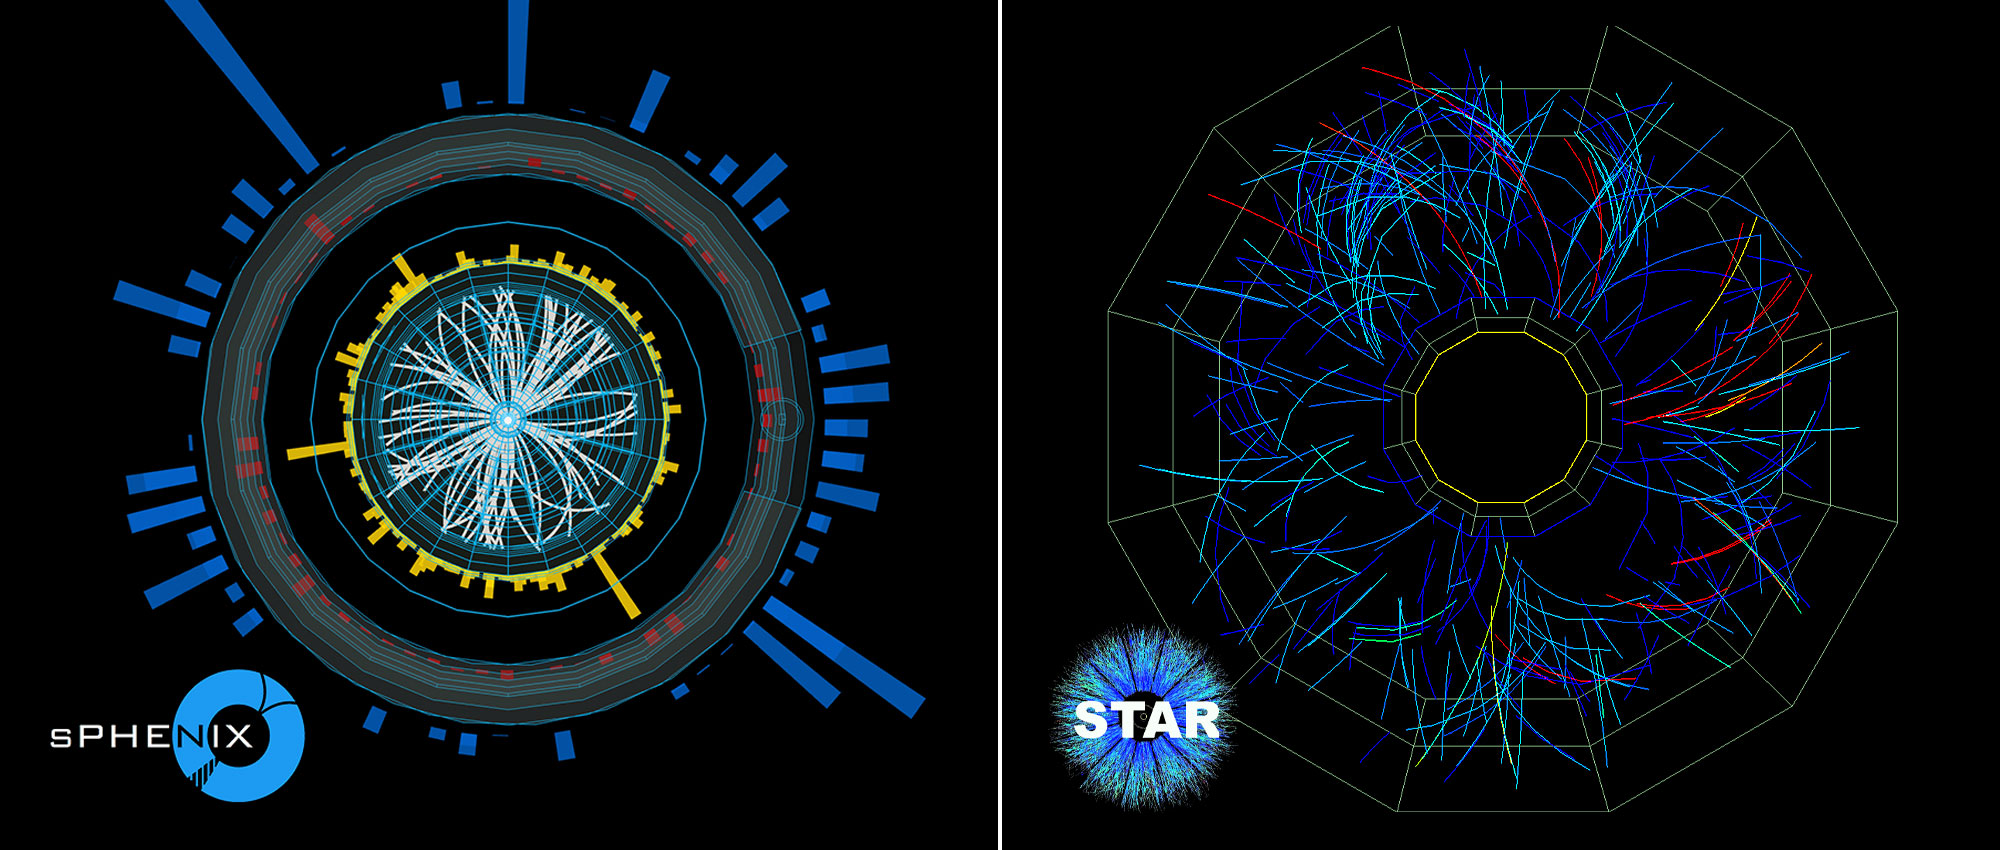
\includegraphics[width=\linewidth]{figures/sphenix-star-events-star-final-hr.jpg}
	\caption[Final O+O collisions recorded by sPHENIX and STAR]{Some of the final O+O collisions at \(\sqrt{s_\mathrm{NN}} = 200\)~GeV captured by the sPHENIX and STAR detectors at the RHIC~\cite{RHICLastRun}.}
	\label{fig:Final}
\end{figure}

\subsection{From stable matter to little bangs}
Before collisions, the nuclei have to be created first by taking the corresponding atoms and stripping off all their electrons, and pre-accelerated in the injector complex shown in Fig.~\ref{fig:AGS}. 
%
That process looks different for different nuclei. 
%
\begin{figure}
	\centering
	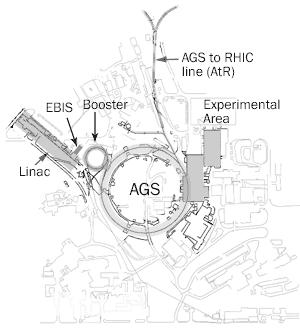
\includegraphics[width=0.5\linewidth]{figures/ags-complex}
	\caption[The RHIC injector complex]{Schematic view of the RHIC injector complex: the Linac (protons) and EBIS (heavy ions) sources, the Booster, the AGS, and the AGS-to-RHIC (AtR) transfer line that carries the beams to RHIC.}
	\label{fig:AGS}
\end{figure}
%
\begin{itemize}
	\item \textbf{For protons} it is \emph{Optically Pumped Polarized \(H^-\) Ion Source (OPPIS)} fed into the \emph{Linear Accelerator (LINAC)}. The LINAC accelerates them to \(\sim 200\)~MeV and injects into the \emph{Booster Synchrotron} at which point, the two electrons are stripped away by a carbon foil. They are accelerated to up to 2.5 GeV and fed into the \emph{ Alternating Gradient Synchrotron (AGS)} which accelerates the proton beam to about 25 GeV.
	\item \textbf{For heavy-ions} like $\rm ^{197}_{79}Au$, a \emph{Laser Ion Source (LION)} extracts \(Au^+\) ions using laser ablation, which go into \emph{Electron Beam Ion Source (EBIS)} which ionizes them to \(Au^{32+}\) and accelerates them to 2 MeV per nucleon using electron beams.  Then they enter the booster synchrotron which accelerates them to about 95 MeV per nucleon. While exiting from the synchrotron, the atoms are stripped of more electrons by passing them through a stripping foil, and atoms in the $\rm Au^{77 + }$ state are fed to the AGS.  The AGS accelerates the Au ions to 8.86 GeV per nucleon, and the final two K-shell electrons are stripped when they leave it. 
	%Resulting beam of $\rm Au^{79 + }$ nuclei that are transported in the \emph{AtR (AGS-to-RHIC)} beampipe to the RHIC storage rings.
\end{itemize}
When the ion beam reached top speed in the AGS, it was taken down another beamline called the AGS-to-RHIC (AtR) transfer line. At the end of this line, a switching magnet sent the ion bunches down each of two beamlines to fill RHIC's two ion storage rings. Bunches directed left filled the clockwise RHIC ring (blue) while those directed right traveled counterclockwise in the second RHIC ring (yellow). In the rings, superconducting radio-frequency (RF) cavities accelerate the ion bunches to energies of 100 GeV per nucleon for heavy ions (255 GeV for protons), with four cavities operating at 28.15 MHz to generate standing waves of electric fields for the acceleration and ten 197 MHz cavities maintaining beam stability during storage. Superconducting dipole magnets with 3.5 T fields keep the beams on a circular path, while quadrupole magnets focus the ion beams. A total of 1,740 superconducting magnets are used in the two rings at RHIC, cooled by liquid Helium at $< 4.6$ K. An aerial view of the RHIC complex with the different subsystems is shown in Fig.~\ref{fig:RHIC-AGS}. 
\begin{figure}
	\centering
	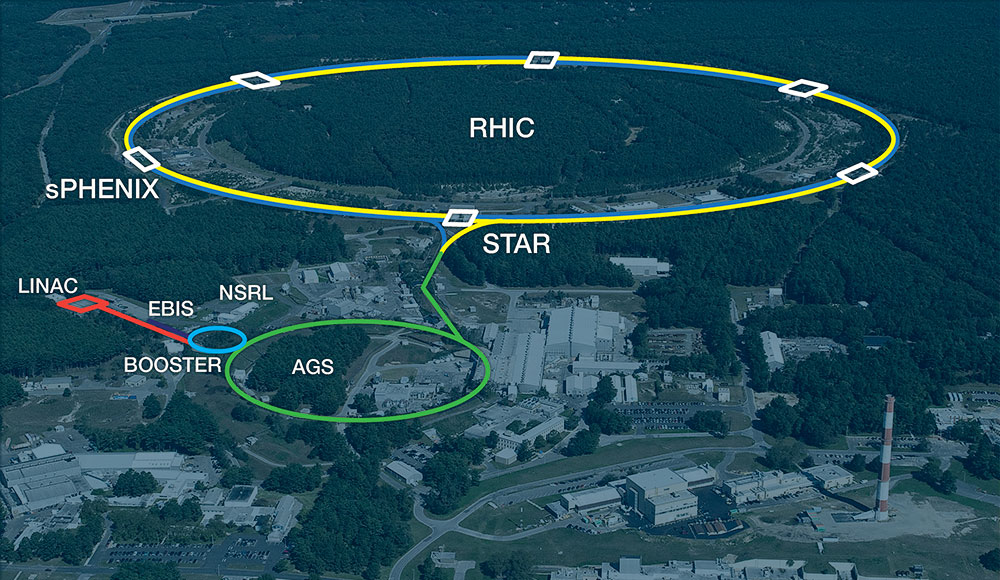
\includegraphics[width=\linewidth]{figures/rhic-aerial-hr.jpg}
	\caption[Aerial view of the RHIC complex]{An aerial view of the Relativistic Heavy Ion Collider (RHIC), showing the locations of the facilities used for accelerating different ions, and the positions of the STAR and sPHENIX detectors~\cite{RHICRun23}.}
	\label{fig:RHIC-AGS}
\end{figure}

There were six interaction regions (IR) around the RHIC complex, where the two beams crossed and detectors could be placed. Four such detectors existed during RHIC's operation: At 10 o'clock and 2 o'clock, the PHOBOS and BRAHMS experiments operated only for the first few years of RHIC (ending in 2006). At 8 o’clock, the PHENIX experiment collected data from 2000 to 2016 and was then transformed into the sPHENIX detector which began operations in 2023. STAR sat at the 6 o'clock position, and was the only experiment to run for all 25 years of RHIC's existence.

\section{The STAR detector}
\label{sec:STAR}
STAR~\cite{ACKERMANN2003624} was designed to provide hermetic coverage around the interaction point, emphasizing precise tracking capabilities in high multiplicity environments, for its main physics mission of obtaining a fundamental understanding of the microscopic structure of QCD interactions at high energy densities.
%\begin{figure}[h]
%	\centering
%	\label{fig:STARSchematic}
%	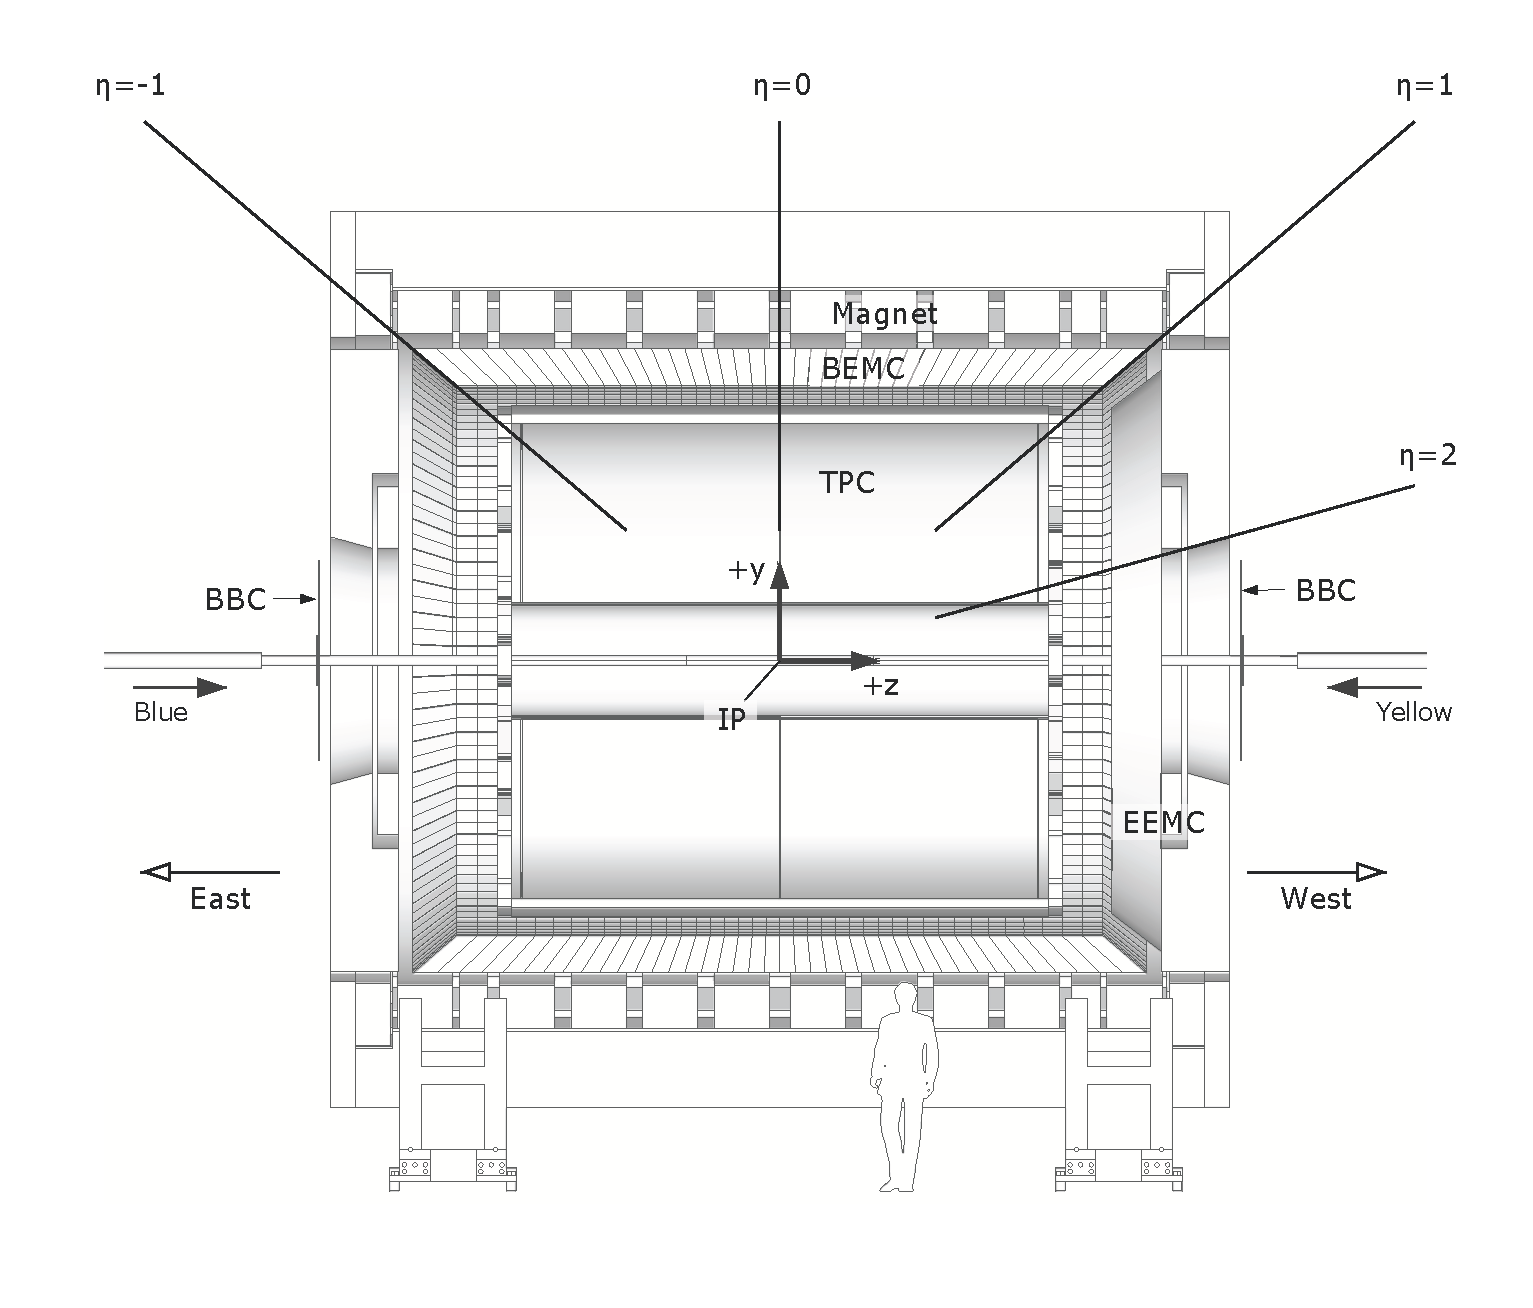
\includegraphics[width=0.8\linewidth]{figures/star_cutout.eps}
%	\caption{Illustration of the STAR Coordinate System.}
%\end{figure}

\begin{figure}
	\centering
\begin{tikzpicture}
	\node[anchor=south west, inner sep=0](image) at (0,0) {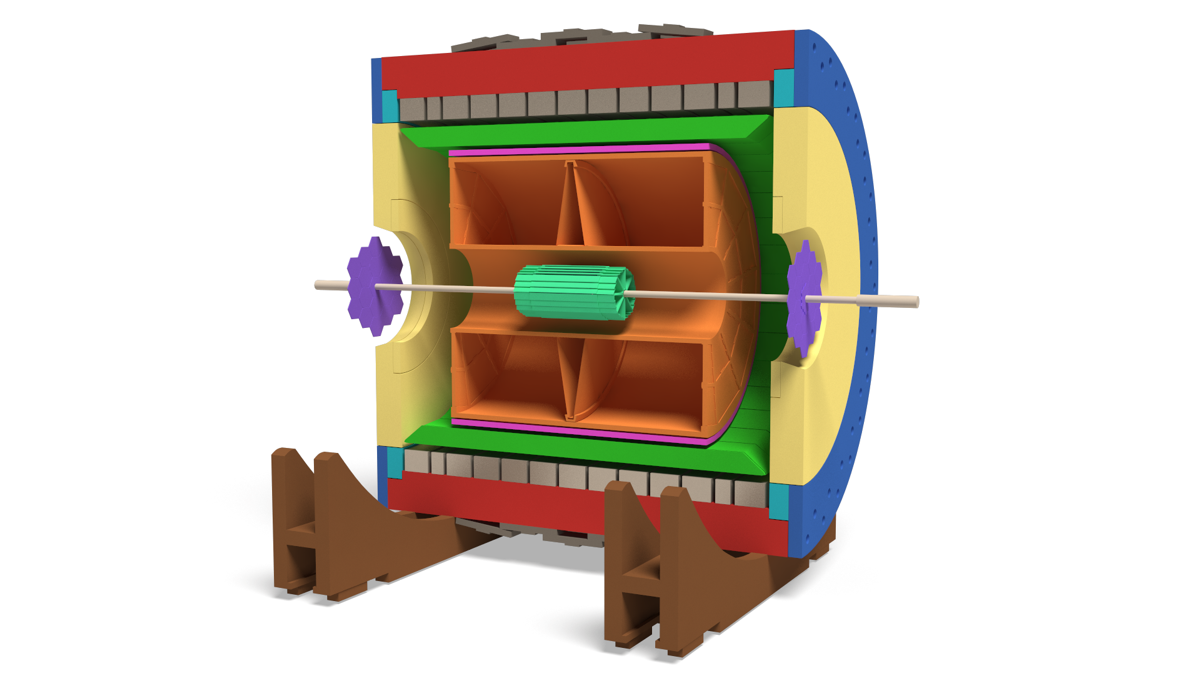
\includegraphics[width=\linewidth]{figures/STAR.png}};
	\node [anchor=west] (bemc) at (11.5,2.5) {BEMC};
	\node [anchor=west] (bbc) at (12,4.5) {BBC};
	\node [anchor=west] (tpc) at (2.5,6) {TPC};
		\node [anchor=west] (hft) at (2.5,3.5) {HFT};
		\node [anchor=west] (mag) at (2.5,8) {Solenoid};
		\node [anchor=west] (tof) at (12,7) {TOF};
				\node [anchor=west] (mtd) at (9, 9) {MTD};
	
	\begin{scope}[x={(image.south east)},y={(image.north west)}]
		\draw [-stealth, line width=1pt] (bemc) to (0.54,0.32);
				\draw [-stealth, line width=1pt] (bbc) to (0.665,0.52);
		\draw [-stealth, line width=1pt] (tpc) to (0.43,0.7);
				\draw [-stealth, line width=1pt] (hft) to (0.47,0.58);
				\draw [-stealth, line width=1pt] (mag) to (0.43,0.84);
				\draw [-stealth, line width=1pt] (tof) to (0.54,0.78);
			\draw [-stealth, line width=1pt] (mtd) to (0.54,0.96);
	\end{scope}
\end{tikzpicture}
\caption[Schematic of the STAR detector]{Schematic of the STAR detector, depicting the various detector subsystems.}
\label{fig:STARDetector}
\end{figure}

It was a highly versatile, multipurpose detector with several subsystems used for triggering, tracking and identifying the particle species for charged tracks, and calorimetry. These subsystems were surrounded by a room-temperature solenoid magnet 6.2 m long and 5.26 m in diameter, which generated a magnetic field of 0.5 T in the detector volume. The detector was cylindrical, with full coverage in the azimuthal direction in the mid-rapidity region along with wide coverage in pseudorapidity. A schematic diagram of the STAR detector with its various detector subsystems is shown in Fig.~\ref{fig:STARDetector}. As the only experiment that ran for the whole lifetime of RHIC, STAR underwent major upgrades that augmented its tracking capabilities and increased its acceptance in the forward rapidity regions. The main detectors used for the analyses of this thesis were the \emph{Time Projection Chamber } (TPC) and \emph{Barrel Electromagnetic Calorimeter} (BEMC). 

\subsection{Detector coordinate system}
\label{sec:detCoordSys}
Before the components of the STAR detector system are described, this section introduces the coordinate system used for the calculations involved. STAR is cylindrical around the beamline, so a convenient choice for \(z\)-axis is the beamline going east-west. The origin \(z=0\) is set at the \emph{Interaction Point} (IP), center of the detector volume, as shown in Fig.~\ref{fig:detcoords}.

 The kinematics of an ultra-relativistic particle are described by its four-momentum, \((E, p_\mathrm{x}, p_\mathrm{y}, p_\mathrm{z})\). However, these coordinates are not additive under Lorentz boosts in the \(z\)-direction, making calculations involving relativistic entities somewhat unwieldy.  Since \(p_\mathrm{x}, p_\mathrm{y}\) are already invariant under Lorentz boosts along the \(z\)-axis, they can simply be converted to the convenient cylindrical coordinates
 \begin{equation}
 	p_\mathrm{T} = \sqrt{p_\mathrm{x}^2 + p_\mathrm{y}^2},\quad \phi = \arctan(\frac{p_\mathrm{y}}{p_\mathrm{x}}) 
 \end{equation}
 Energy (\(E\)) can be replaced with the particle's mass (\(m\)), or transverse mass \(m_\mathrm{T} = \sqrt{p_\mathrm{T}^2 + m^2}\).
 The \(z\)-coordinate can be made additive under Lorentz Boosts along \(z\)-axis by representing a particle's direction along the \(z\)-axis by \emph{rapidity}
\begin{equation}
		y  = \frac{1}{2} \ln \frac{E + p_z}{E - p_z} 
\end{equation}

However, \(y\) is mass dependent, and most detectors do not provide robust particle identification in all kinematic ranges. The \(z\)-direction in a detector is therefore usually described using \emph{Pseudorapidity}, which is the massless limit of rapidity
\begin{equation}
	\eta = \lim_{m\to 0} y= \frac{1}{2} \ln \frac{p + p_z}{p - p_z}  = -\ln(\tan\frac{\theta}{2})
\end{equation}
where \(\theta\) is the polar angle between the particle's direction and the \(z\)-axis as shown in Fig.~\ref{fig:detcoords}. Thus a particle's four-momentum is given by \((m_\mathrm{T}, p_\mathrm{T}, \eta, \phi)\) or \((p_\mathrm{T}, \eta, \phi, m)\).  See App.~\ref{sec:coordSysAppendix} for a more detailed derivation of coordinates.

\begin{figure}
	\centering
	\detectorCoordinateSystem
	\caption[The \((p_\mathrm{T}, \eta, \phi)\) coordinate system of a collider detector]{The \((p_{\rm T}, \eta, \phi)\) coordinate system, drawn for a cylindrical
		collider detector. The beam axis defines \(z\) and the interaction point (IP) sits at
		the origin. A particle of momentum \(\vec{p}\) is described by its transverse momentum
		\(\vec{p}_{\rm T}\), its azimuthal angle \(\phi\) in the transverse plane, and its
		pseudorapidity \(\eta\), fixed by the polar angle \(\theta\) with respect to the beam.}
	\label{fig:detcoords}
\end{figure}

\subsection{TPC} \label{TPC}
 Time Projection Chamber (TPC)~\cite{Anderson_2003} was the primary tracking detector for STAR, providing particle identification and momentum information for charged tracks by measuring their ionization energy loss (dE/dx) inside the TPC volume. As shown in Fig.~\ref{fig:TPC} the TPC was a cylindrical detector 420 cm long with an outer (inner) radii of 200 (50) cm, concentric to the 0.5 T solenoid. Its acceptance covered a pseudorapidity range of $|\eta| < 1.0$, along with full azimuthal coverage. Charged tracks could be reconstructed from about 0.1~GeV/\(c\), below which they curled up before reaching the TPC, to about 30~GeV/\(c\). At the lowest momenta, however, the tracking efficiency drops and multiple scattering degrades the momentum resolution, which is why the analyses in this thesis use tracks above 0.2~GeV/\(c\). Particles could be identified by their ionization energy loss mainly below about 1~GeV/\(c\), as discussed below.
\begin{figure}
	\centering
	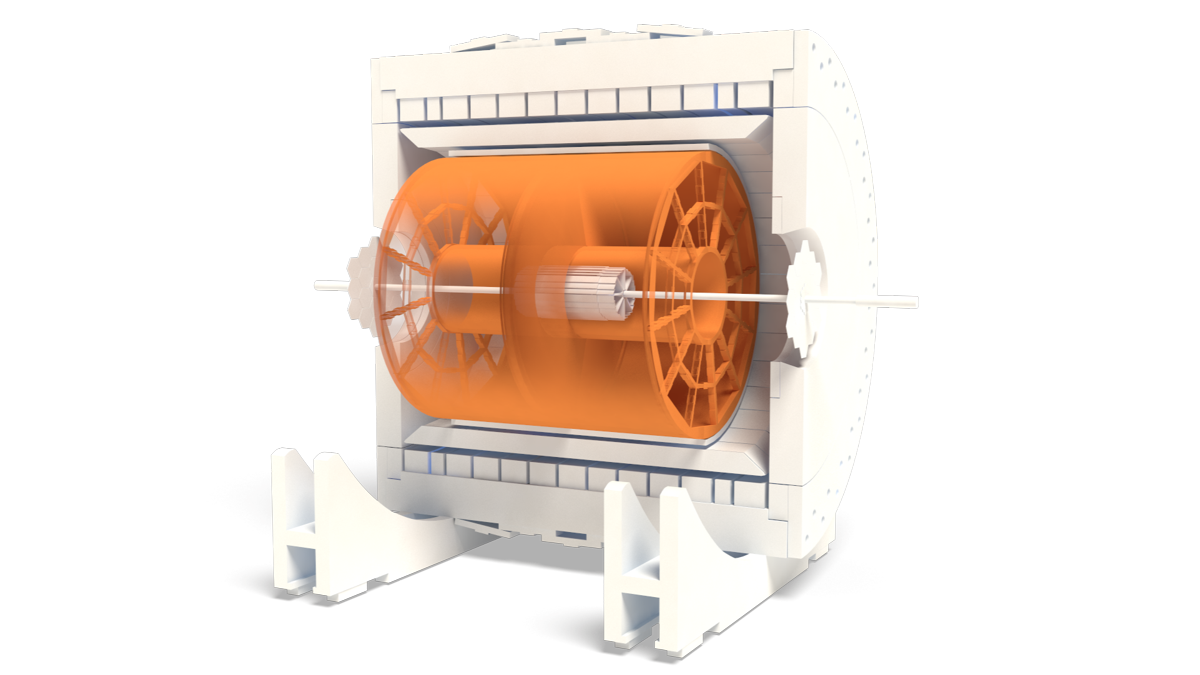
\includegraphics[width=\linewidth]{figures/TPC.png}
	\caption[The STAR Time Projection Chamber]{The Time Projection Chamber at STAR, shown in orange. Taken from~\cite{STARSubSystems}.}
	\label{fig:TPC}
\end{figure}
The TPC volume contained an ionizable gas mixture called P10 (10 \% methane, 90 \% argon), chosen for its high drift velocity of 5.45 $\rm cm/\mu s$ in the well-defined, uniform electric field of $\approx 135$ V/cm at STAR. 
%
The uniform electric field was defined between the thin conductive central membrane at z = 0 maintained at 28 kV acting as a cathode, and the two end caps each 210 cm away from the center at 0 V acting as anodes. 
%
The drift velocity could change over time with atmospheric pressure fluctuations; therefore, it was calibrated with lasers every few hours during data-taking. 
%
To minimize contamination by impurities like oxygen and water vapor, the gas was maintained at 2 mbar above atmospheric pressure. 

\begin{figure}
	\centering
	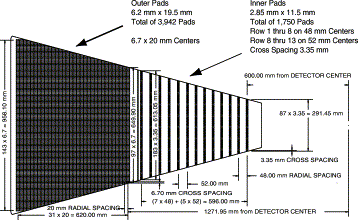
\includegraphics[width=0.7\linewidth]{figures/TPCAnode.png}
	\caption[A sector of the TPC]{One of the twelve sectors of the TPC. Taken from~\cite{Anderson_2003}.}
	\label{fig:TPCAnode}
\end{figure}

The ionization trails left by charged particles were read out by Multi-Wire Proportional Counters (MWPCs) with a segmented pad plane.
%
As particles ionized the TPC gas, the freed electrons drifted toward the MWPCs under the effect of the electric field. 
%
Signal contamination was prevented using a gated grid that initially restricted electron flow, opening only if a collision was deemed significant, allowing electrons to enter the MWPCs. 
%
Positive ions generated inside the MWPC were prevented from entering the TPC’s drift volume using shield wires. 
%
The electrons passed the shield wires and were rapidly accelerated near the anode wires, creating avalanches through secondary ionization and amplifying the signal by a factor of 1,000 to 3,000. These avalanches induced signals in the surrounding pads without direct contact with the electrons. The MWPC pads detected the x-y position based on pad geometry — 3,942 pads across 32 rows in the outer sector and 1,750 pads in 13 rows in the inner sector. One such anode sector is shown in Fig.~\ref{fig:TPCAnode}. The z information was then derived from the drift time of the electrons, measured relative to the collision time \(t_0\) provided by fast detectors such as the Vertex Position Detector (VPD)~\cite{Llope:2014nva}, and their calibrated drift velocity. The typical resolution for position measurements from the TPC was roughly 1 cm.
\begin{figure}
	\centering
	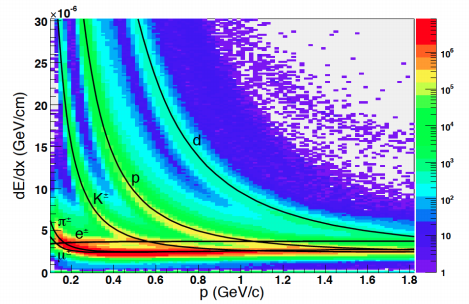
\includegraphics[width=\linewidth]{figures/dEdxVsp.png}
	\caption[Ionization energy loss in the TPC as a function of momentum]{The ionization energy loss for charged particles from TPC as a function of momenta. The letters represent different particles: $\mu^{\pm}$ for muons, $e^{\pm}$ for electrons, $\pi^{\pm}$ for pions, $K^{\pm}$ for Kaons, p for protons, and d for deuterons. The solid lines are the expected value of dE/dx for the corresponding particle species from the Bichsel function~\cite{BICHSEL2006154}.}
	\label{fig:dEdx}
\end{figure}

For a charged particle track, maximum of 45 hits could be recorded, which were fitted to a helix to calculate the particle momentum. Particles with momentum below 100 MeV/\(c\) curved too tightly in the magnetic field to reach the TPC. At high momentum the opposite problem arose: the tracks were nearly straight, and their momentum followed from a small sagitta. Over the roughly 1.5~m lever arm of the TPC, the sagitta was about 1~mm for a 40~GeV/\(c\) track and 0.7~mm for a 60~GeV/\(c\) track, a difference comparable to the precision of the hit positions, so the two momenta could hardly be distinguished. The relative momentum resolution, about 2\% at low momentum, therefore grew in proportion to the momentum and became too large above about 30~GeV/\(c\). The direction of curvature gives the charge of the track. Energy loss as a function of distance traveled, dE/dx for a track was extracted using energy loss measured by a series of pads in the TPC. Fig.~\ref{fig:dEdx} shows a typical plot of measured dE/dx as a function of momentum. For a given particle species with known momenta, the dE/dx curves are given by the Bichsel function~\cite{BICHSEL2006154} which are shown as solid lines in Fig.~\ref{fig:dEdx}. For each particle species, the band has non-zero thickness due to the finite momentum resolution, and selection criteria based on simulations are used to assign particle ID. The momentum up to which two species could be separated depended on the pair. Muons and pions, of similar mass, overlapped at all but the lowest momenta, pions and kaons could be separated up to about 0.7~GeV/\(c\), and protons from both up to about 1~GeV/\(c\), while the band of the heavier deuterons remained distinct to higher momenta.

\subsection{BEMC} \label{BEMC}

The STAR Barrel Electromagnetic Calorimeter (BEMC) \cite{BEDDO2003725} was designed to measure particle energies, particularly for electron and neutral particle identification.
%
The BEMC was a fast detector, used as a trigger to select events containing a hard process. 
%
It also provided the neutral component of the jet energy that couldn't be reconstructed by the TPC in jet-related measurements. 
%
As shown in Fig.~\ref{fig:BEMC}, it was a cylindrical detector located between the TPC and magnet coils. 
%
It covered the pseudorapidity range $|\eta| < 1$ and the full azimuth range (\(0 \leq \phi \leq 2\pi\)), matching the TPC's coverage.

\begin{figure}
	\centering
	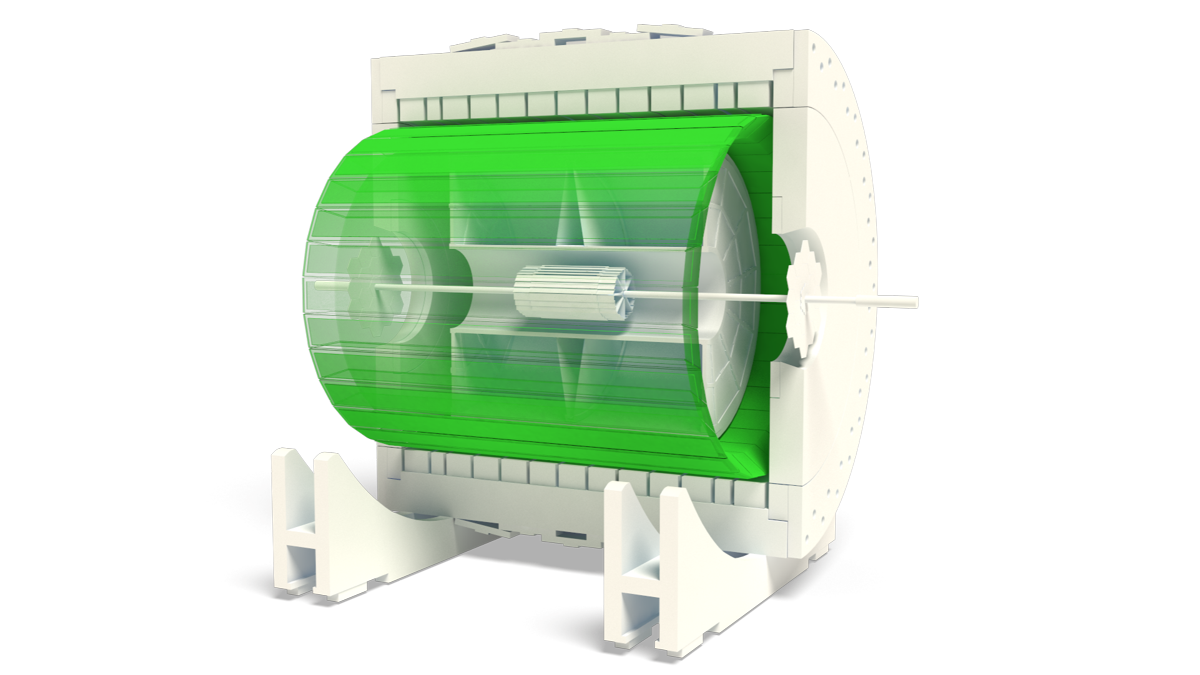
\includegraphics[width=\linewidth]{figures/BEMC.png}
	\caption[The STAR Barrel Electromagnetic Calorimeter]{The Barrel Electromagnetic Calorimeter at STAR, shown in green. Taken from \cite{STARSubSystems}.}
	\label{fig:BEMC}
\end{figure}

The BEMC had inner and outer radii of  223.5 cm and 263 cm respectively and consisted of 120 modules, each containing 40 towers, totaling 4800 towers. 
%
Each of the towers covered a range of $\Delta \eta \times \Delta \phi = 0.05 \times 0.05$, approximately 10 cm × 10 cm near $\eta = 0$, growing slightly with increasing $|\eta|$ due to their projective geometry toward the center of the detector ($z = 0$). 
%
Each tower was built with 20 alternating layers of 5-mm thick lead, acting as absorbers to initiate electromagnetic showers, and 21 layers of plastic scintillators, which detected the photons produced by these showers. 
%
Together, the layers created a depth of around 20 radiation lengths ($\rm X_0$), allowing the calorimeter to capture nearly all of the energy from electromagnetic showers. 
%
This depth was enough to contain 95 \% of the energy from electrons and photons above 1 GeV. 
%
Within these layers, the shower’s energy was most concentrated around 5-7 radiation lengths in, where the Shower Maximum Detector (SMD), a gas (90 \% Argon, 10 \% $\rm CO_{2}$)-filled proportional counter improved the spatial resolution to help differentiate between electromagnetic and hadronic shower profiles.
%
The BEMC had an energy resolution that improved with particle energy, around 17\% for 1.5 GeV electrons and 10\% for 3 GeV electrons in head-on Au+Au collisions.
%
 This follows the typical calorimetric trend in which the relative energy resolution improves as the energy increases ($\sigma_{E}/E \approx 1.5 \% + 15 \% /\sqrt{E}$), complementing the TPC, whose relative momentum resolution degrades with increasing momentum ($\sigma_{p_\mathrm{T}}/p_\mathrm{T} \propto p_\mathrm{T}$).
\subsection{Trigger and luminosity detectors} \label{sec:triggerDetectors}
Besides the TPC and the BEMC, three fast forward detectors enter the analyses of this thesis, through the minimum-bias trigger, the online vertex selection and the monitoring of the luminosity.
%
Their signals were available for every bunch crossing and were combined by the STAR trigger system to decide which collisions were recorded~\cite{Bieser:2002ah}.

\subsubsection{Vertex Position Detector (VPD)} \label{VPD}
The VPD~\cite{Llope:2014nva} consisted of two identical assemblies mounted around the beam pipe 5.7~m from the center of STAR on either side, each with 19 detectors covering about half of the solid angle in \(4.24 \leq |\eta| \leq 5.1\) (Fig.~\ref{fig:VPD}, top).
%
\begin{figure}
	\centering
	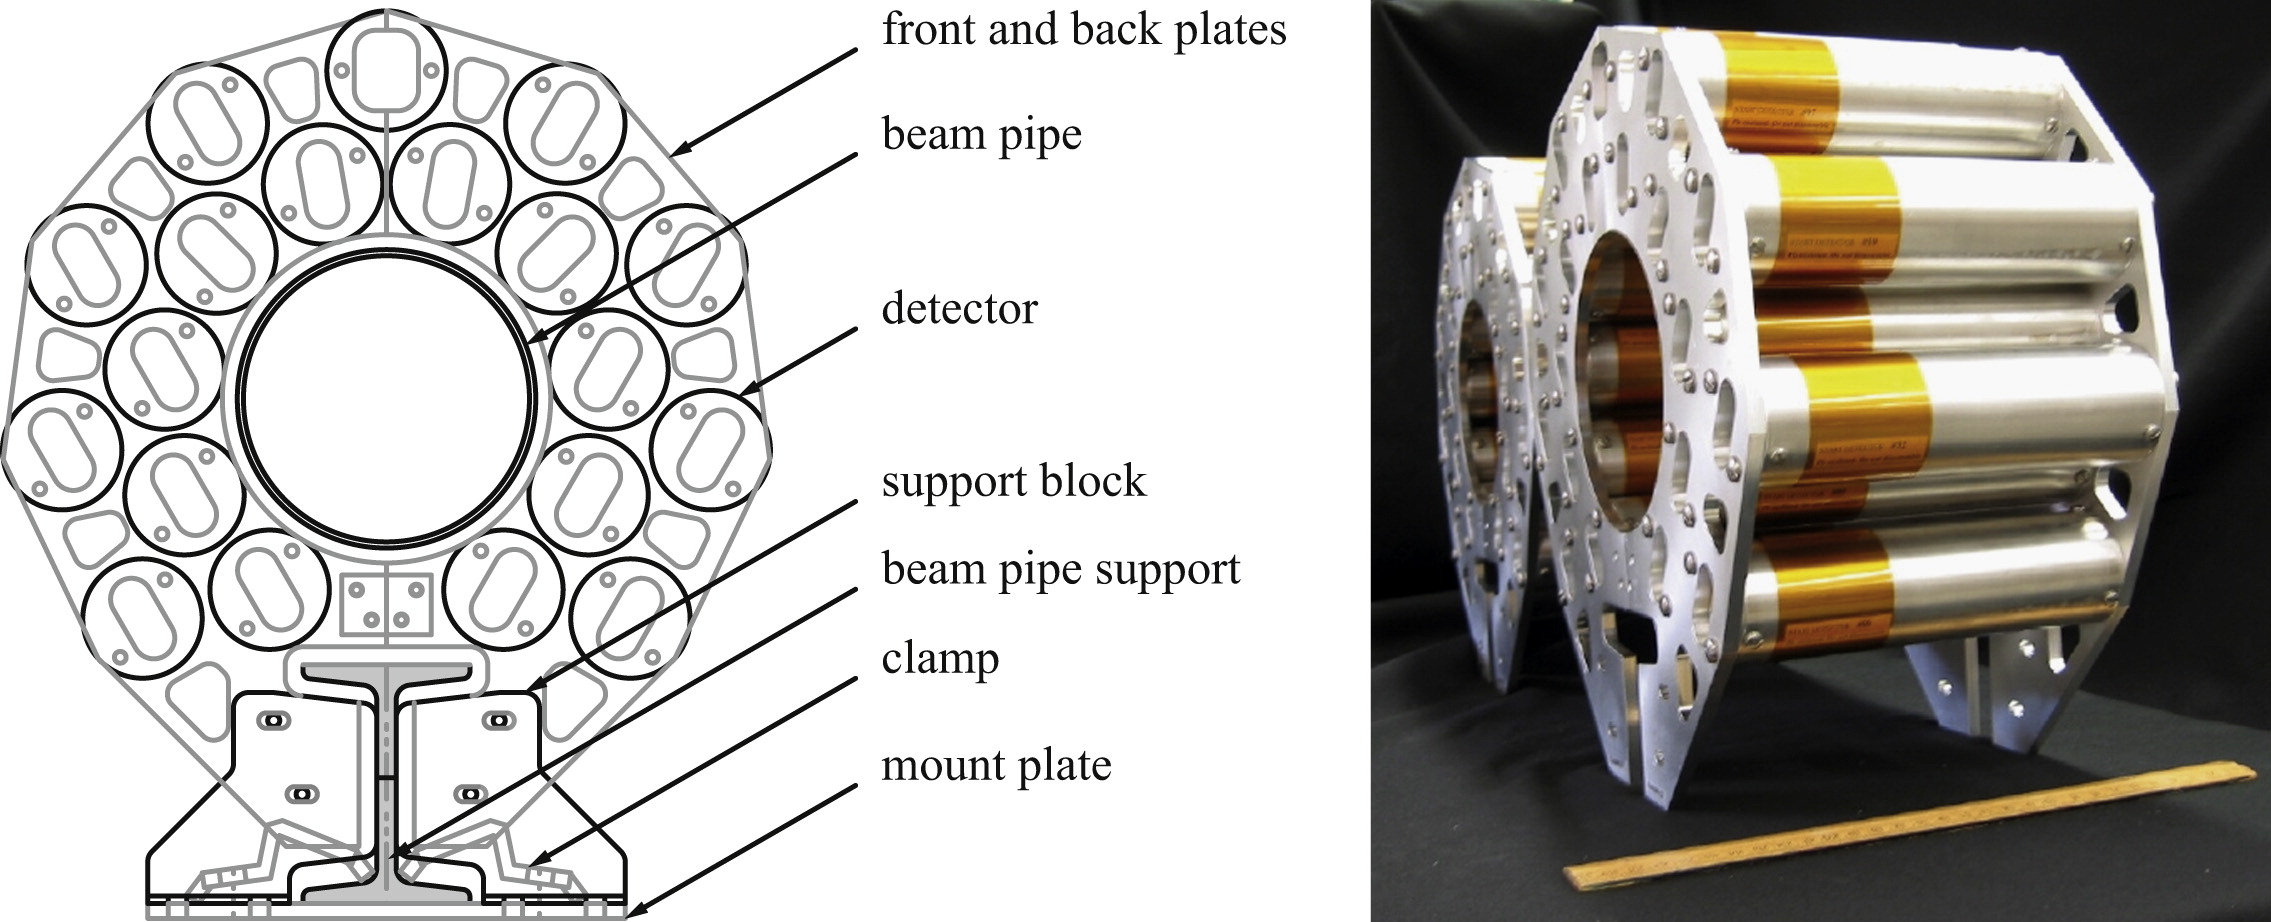
\includegraphics[width=\linewidth]{figures/VPD_fig2.jpg}\\[1ex]
	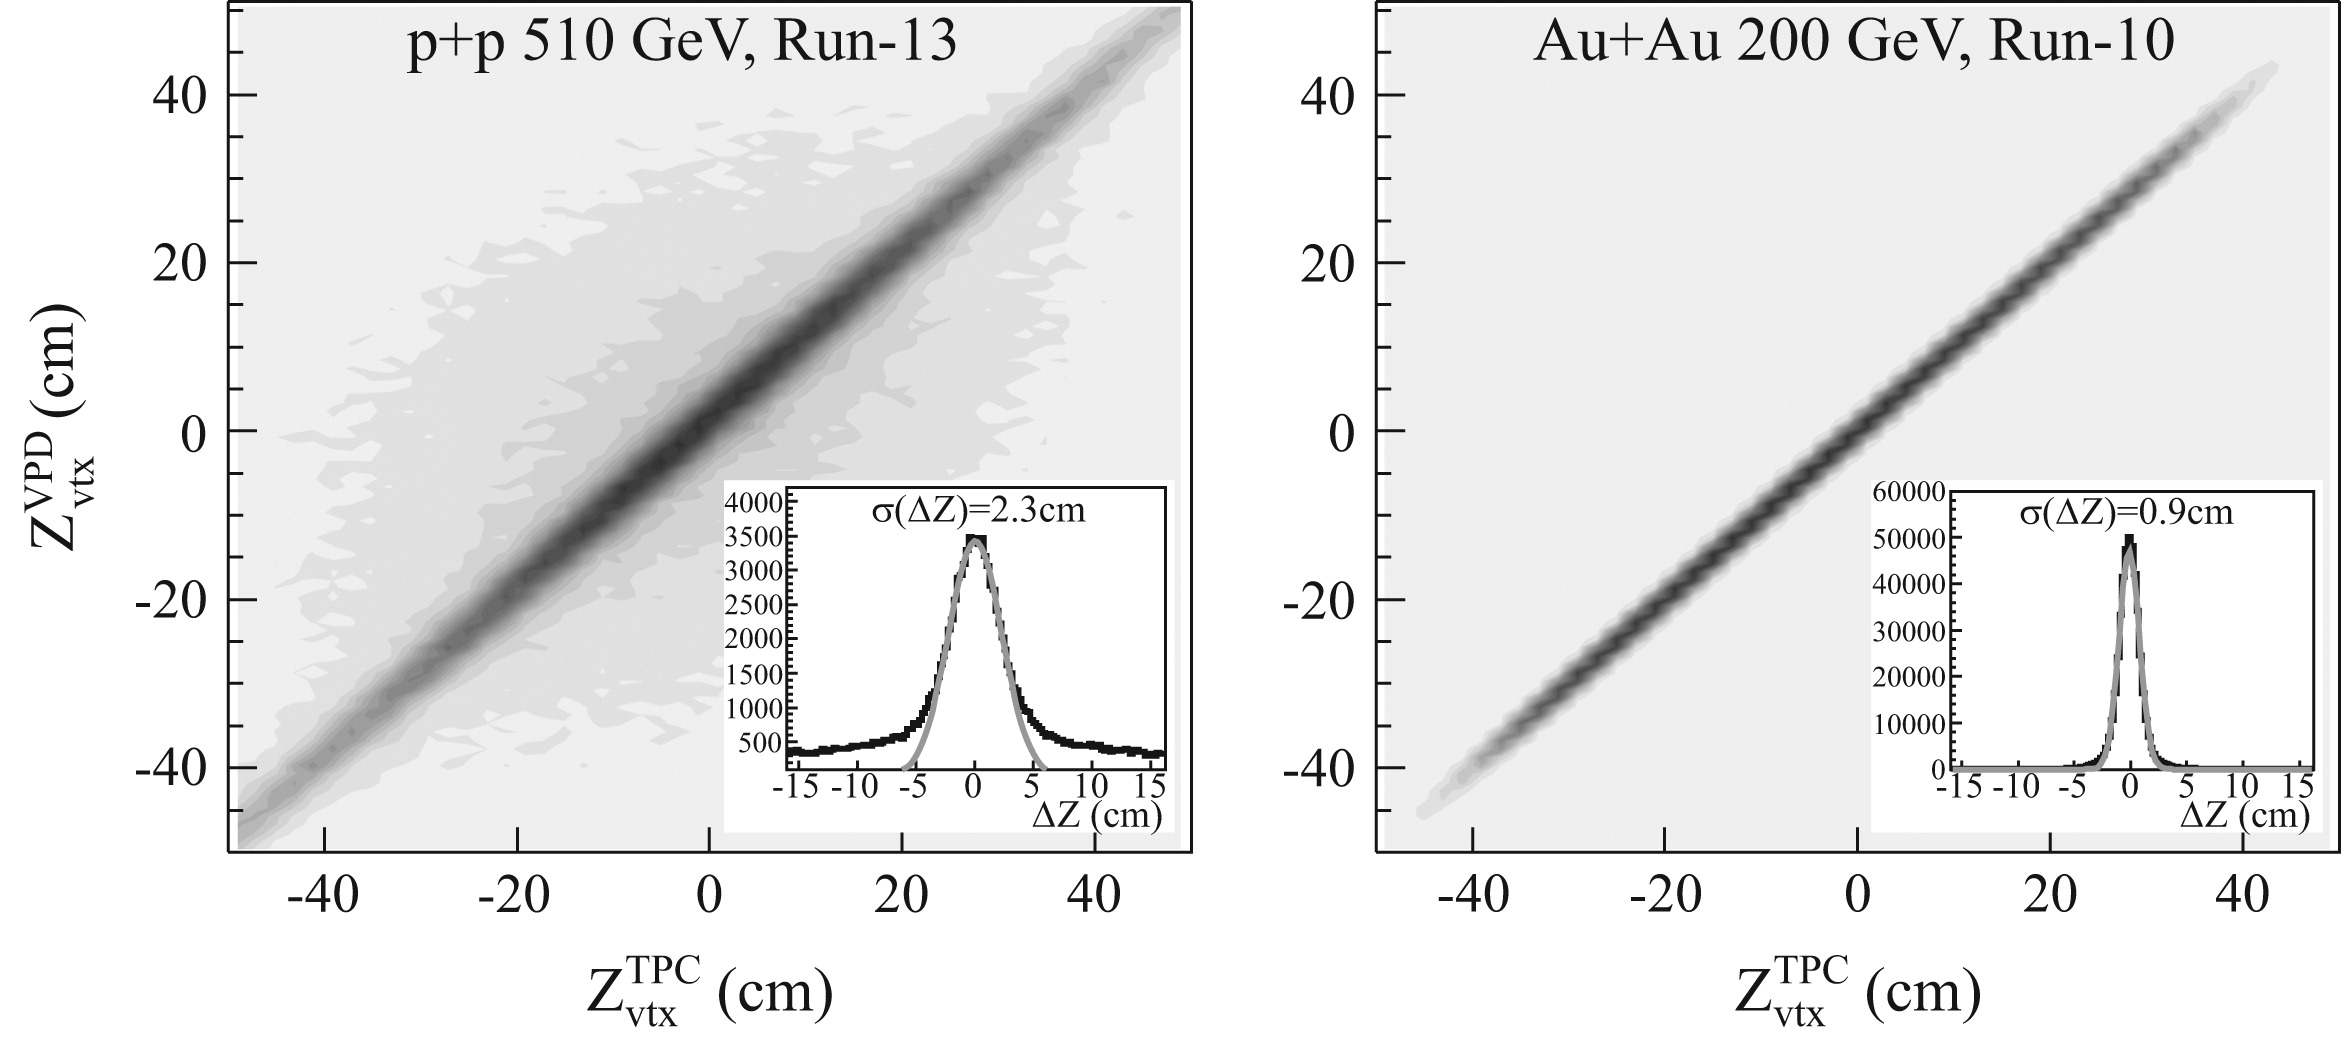
\includegraphics[width=\linewidth]{figures/VPD_fig6.jpg}
	\caption[The STAR Vertex Position Detector]{(Top) Schematic front view of one VPD assembly around the beam pipe (left) and photograph of the two assemblies (right). (Bottom) Primary-vertex position along the beam measured by the VPD versus the one reconstructed from TPC tracks, in \(p+p\) collisions at \(\sqrt{s} = 510\)~GeV (left) and \AuAu collisions at \sNN{200}{GeV} (right); the insets show the distributions of their difference. Taken from~\cite{Llope:2014nva}.}
	\label{fig:VPD}
\end{figure}
%
Each detector was a lead converter followed by a fast plastic scintillator read out by a photomultiplier tube, and measured the arrival time of the nearly light-speed particles produced at forward rapidity.
%
The difference between the arrival times at the east and west assemblies gives the position of the collision vertex along the beam, \(v_z = c\,(t_\mathrm{east} - t_\mathrm{west})/2\), with a resolution of about 1~cm in \AuAu collisions (Fig.~\ref{fig:VPD}, bottom), and their average gives the start time of the collision to a few tens of picoseconds, which the TPC uses as its time reference (Sec.~\ref{TPC}).
%
The VPD coincidence was the main input to the minimum-bias trigger in \AuAu collisions, and the online vertex position it provides defines the VPDMB5 and VPDMB30 triggers of Ch.~\ref{ch:jhcorr}, which require \(|v_z| < 5\) and 30~cm, respectively.

\subsubsection{Beam-Beam Counters (BBC)} \label{BBC}
The BBCs were two annuli of scintillator tiles mounted around the beam pipe beyond the east and west pole tips of the STAR magnet, 3.74~m from the center of the detector~\cite{Kiryluk:2005gg}.
%
Their inner ring of small hexagonal tiles (Fig.~\ref{fig:BBC}) covered \(3.4 < |\eta| < 5.0\) over the full azimuth, and was surrounded by larger tiles at smaller \(|\eta|\).
%
\begin{figure}
	\centering
	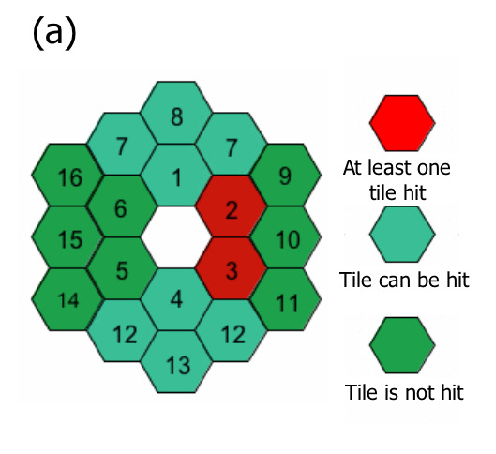
\includegraphics[width=0.5\linewidth, trim={0 0 0 31bp}, clip]{figures/jkiryluk_fig1a.pdf}
	\caption[The small tiles of the STAR Beam-Beam Counters]{Schematic view of the small hexagonal tiles of one BBC around the beam pipe (central opening), labeled by their photomultiplier tubes. The colors show an example event of the local polarimetry measurement of Ref.~\cite{Kiryluk:2005gg}, a charged particle hitting tiles on one side (red). Taken from~\cite{Kiryluk:2005gg}.}
	\label{fig:BBC}
\end{figure}
%
A coincidence of hits in the east and west BBCs within the time window of a bunch crossing signals an inelastic collision; the BBCs provided the minimum-bias trigger and the relative luminosity measurement in \pp collisions, and served as local polarimeters for the polarized proton beams~\cite{Kiryluk:2005gg}.
%
In the \AuAu minimum-bias trigger of Ch.~\ref{ch:jhcorr}, the BBC signals are combined with those of the VPD and the ZDCs.

\subsubsection{Zero Degree Calorimeters (ZDC)} \label{ZDC}
The ZDCs~\cite{Adler:2000bd} were identical hadronic calorimeters built for all RHIC experiments and placed about 18~m on either side of the interaction point, downstream of the dipole magnets that separate the two beams (Fig.~\ref{fig:ZDC}).
%
\begin{figure}
	\centering
	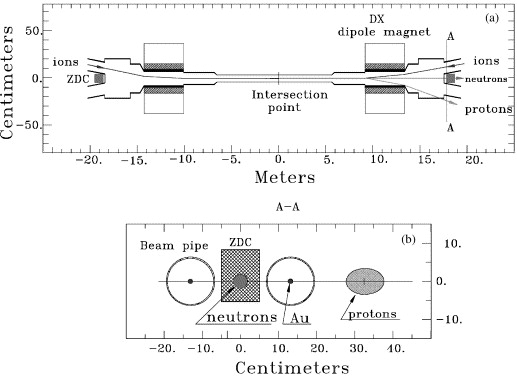
\includegraphics[width=0.75\linewidth]{figures/ZDC_fig1.jpg}
	\caption[Location of the Zero Degree Calorimeters]{(a) Plan view of the collision region, with the ZDCs behind the DX dipole magnets, which bend the ion beams and the protons away from the neutrons. (b) Beam's-eye view at the ZDC location (section A--A in (a)), showing the neutrons hitting the ZDC between the two beam pipes, while the deflected protons miss it. Taken from~\cite{Adler:2000bd}.}
	\label{fig:ZDC}
\end{figure}
%
The magnets bend the beams and the charged fragments of the nuclei away, so that only neutral particles, mostly the spectator neutrons that evaporate from the colliding nuclei within about 2~mrad of the beam axis, reach the calorimeters.
%
Each ZDC was built from tungsten absorber plates interleaved with optical fibers that collect the Cherenkov light of the hadronic shower, arranged in modules along the beam, and measured the total energy of these neutrons, i.e.\ their number.
%
The coincidence of the two ZDCs is a minimum-bias selection of heavy-ion collisions, and its rate (ZDCx) serves as a monitor of the luminosity; in Ch.~\ref{ch:jhcorr} it is part of the minimum-bias trigger and is used in the run-by-run quality assurance (Sec.~\ref{sec:JHEventSel}).

%
%\section{Dijet events}
%In dijet events, two incoming partons, one each from the incoming nuclei scatter off each other and produce two final state partons, which are observed as jets. The two partons are back-to-back and have equal momenta in the processes center of mass frame. A typical process,
%\begin{equation}
%	\mathrm{parton}_i(p_1) + \mathrm{parton}_j(p_2) \rightarrow \mathrm{parton}_k(p_3) + \mathrm{parton}_l(p_4)
%\end{equation}
%Has parton cross-section:
%
%\begin{equation}
%	\frac{E_3E_4d^6\hat{\sigma}}{d^3p_3d^3p_4} = \frac{1}{2\hat{s}}\frac{1}{16\pi^2}\overline{\sum}|\mathcal{M}|^2\delta^4(p_1 + p_2 - p_3 - p_4)
%	\label{eq:partonxsec}
%\end{equation}
%
%Where, \(\overline{\sum}\)  denotes  the average and sum over the spins and colors of initial and final partons \(\{i, j, k, l\}\) and \(\hat{s} = (p_1+p_2)^2\). To get the dijet cross-section, we insert the parton cross-section from Eq. \ref{eq:partonxsec} into  Eq. \ref{eq:factorization}. Assuming the incoming partons are massless and collinear with the beams, \(p_1 = \frac{1}{2}x_1\sqrt{s}(1, 0, 0, 1)\) and \(p_2 = \frac{1}{2}x_2\sqrt{s}(1, 0, 0, -1)\), so that \(\hat{s} = x_1x_2s\),
%
%\begin{align*}
%	\frac{E_3E_4d^6\sigma}{d^3p_3d^3p_4} & = \frac{1}{2s}\frac{1}{16\pi^2} \sum_{\{i,j,k,l\}\subset q\bigcup\bar{q}\bigcup g} \frac{1}{1 + \delta_{kl}} \int dx_1dx_2 \frac{f_i(x_1, \mu^2)}{x_1} \frac{f_j(x_2, \mu^2)}{x_2} \\
%	& \qquad \times\, \overline{\sum}|\mathcal{M}(ij\rightarrow kl)|^2\delta^4(p_1 + p_2 - p_3 - p_4) 
%\end{align*}
%Where \(q\bigcup\bar{q}\bigcup g\) represents all the partonic states \(\{g, u, \bar{u}, d, \ldots\}\). 
%
%%	The four-momentum conserving \(\delta\)-function factorizes into a transverse part and the energy and longitudinal parts, 
%%	
%%	\begin{align*}
%	%	\delta^4(p_1 + p_2 - p_3 - p_4)                                & = \delta^2(\mathbf{p}_{T3} + \mathbf{p}_{T4})\,\delta\left(\tfrac{1}{2}\sqrt{s}(x_1 + x_2) - E_3 - E_4\right)                 \\
%	%	                                                               & \qquad \times\, \delta\left(\tfrac{1}{2}\sqrt{s}(x_1 - x_2) - p_{z3} - p_{z4}\right) \\
%	%	                                                               & = \frac{2}{s}\delta^2(\mathbf{p}_{T3} + \mathbf{p}_{T4})\,\delta\left(x_1 - \tfrac{1}{2}x_T(e^{y_3} + e^{y_4})\right)         \\
%	%	                                                               & \qquad \times\, \delta\left(x_2 - \tfrac{1}{2}x_T(e^{-y_3} + e^{-y_4})\right)
%	%\end{align*}
%	%
%	%Where, \(x_T \equiv 2p_T/\sqrt{s}\) and \(p_T \equiv p_{T, 3} = p_{T, 4}\),
%	%
%	%\begin{equation}
%	%	\frac{d^3\sigma}{dy_3dy_4dp_T^2} = \frac{1}{16\pi s^2}\sum_{\{i,j,k,l\}\subset q\bigcup\bar{q}\bigcup g} \frac{1}{1 + \delta_{kl}} \frac{f_i(x_1, \mu^2)}{x_1}\frac{f_j(x_2, \mu^2)}{x_2} \overline{\sum}|\mathcal{M}(ij\rightarrow kl)|^2
%	%\end{equation}
%	
%	Integrating Eq. \ref{eq:partonxsec} over one of the outgoing partons gives the
%	\emph{single-inclusive} parton cross-section for the other.  Writing
%	\(q \equiv p_1 + p_2 - p_3\),
%	\begin{align}
%		\frac{E_3d^3\hat{\sigma}}{d^3p_3} &= \frac{1}{2\hat{s}}\frac{1}{16\pi^2}\overline{\sum}|\mathcal{M}|^2\int\frac{d^3p_4}{E_4}\,\delta^4(p_1 + p_2 - p_3 - p_4)                              \notag                      \\
%		&=\frac{1}{2\hat{s}}\frac{1}{16\pi^2}\overline{\sum}|\mathcal{M}|^2\int\frac{d^3p_4}{E_4}\,\delta^3(\mathbf{q} - \mathbf{p}_4)\,\delta(q^0 - E_4) \notag \\
%		&= \frac{1}{2\hat{s}}\frac{1}{16\pi^2}\overline{\sum}|\mathcal{M}|^2\,\frac{\delta(q^0 - |\mathbf{q}|)}{|\mathbf{q}|}       \notag \\  
%		&= \frac{1}{2\hat{s}}\frac{1}{16\pi^2}\overline{\sum}|\mathcal{M}|^2\,2\delta(q^2)                  
%	\end{align}
%	We can represent \(q^2\) in terms of partonic Mandelstam variables \(\hat{s} = (p_1+p_2)^2\), \(\hat{t} = (p_1-p_3)^2\) and \(\hat{u} = (p_2-p_3)^2\),
%	
%	\begin{align}
%		\implies \frac{Ed^3\hat{\sigma}}{d^3p}  &= \frac{1}{2\hat{s}}\frac{1}{8\pi^2}\overline{\sum}|\mathcal{M}|^2\delta(\hat{s} + \hat{t} + \hat{u})
%	\end{align}
%	
%	Assuming perfect detector and jet algorithm, the outgoing parton's momentum is the ensuing jet's momentum.
%	\begin{align}
%		\frac{E_Jd^3\sigma}{d^3p_J}  =& \frac{1}{16\pi^2 s}\sum_{\{i,j,k,l\}\subset q\bigcup\bar{q}\bigcup g} \frac{1}{1 + \delta_{kl}}\int_{0}^{1} \frac{dx_1}{x_1}\frac{dx_2}{x_2} f_i(x_1, \mu^2) f_j(x_2, \mu^2) \notag\\ &\times\overline{\sum}|\mathcal{M}(ij\rightarrow kl)|^2\delta(\hat{s} + \hat{t} + \hat{u})
%	\end{align}
%	\begin{sidewaystable}[htbp]
%		\centering
%		\setlength{\tabcolsep}{4pt}
%		\begin{tabular}{
%				>{\centering\arraybackslash}m{2.2cm}
%				>{\centering\arraybackslash}m{2.8cm}
%				>{\centering\arraybackslash}m{2.8cm}
%				>{\centering\arraybackslash}m{2.8cm}
%				>{\centering\arraybackslash}m{2.8cm}
%				>{\centering\arraybackslash}m{6.8cm}
%			}
%			\toprule
%			Process & \multicolumn{4}{c}{Diagrams} & \(\overline{\sum}|\mathcal{M}|^2/(4\pi\alpha_s)^2\) \\
%			\midrule
%			\(qq' \to qq'\)             & \diagqqpT{q'}{q}   &                  &            &          &
%			\(\dfrac{4}{9}\dfrac{\hat{s}^2+\hat{u}^2}{\hat{t}^2}\)                                                   \\
%			\(qq \to qq\)               & \diagqqpT{q}{q}    & \diagqqU{q}      &            &          &
%			\(\dfrac{4}{9}\left(\dfrac{\hat{s}^2+\hat{u}^2}{\hat{t}^2}+\dfrac{\hat{s}^2+\hat{t}^2}{\hat{u}^2}\right)
%			-\dfrac{8}{27}\dfrac{\hat{s}^2}{\hat{u}\hat{t}}\)                                                        \\
%			\(q\bar{q}' \to q\bar{q}'\) & \diagqqbpT{q}{q'}  &                  &            &          &
%			\(\dfrac{4}{9}\dfrac{\hat{s}^2+\hat{u}^2}{\hat{t}^2}\)                                                   \\
%			\(q\bar{q} \to q'\bar{q}'\) & \diagqqbAnn{q}{q'} &                  &            &          &
%			\(\dfrac{4}{9}\dfrac{\hat{t}^2+\hat{u}^2}{\hat{s}^2}\)                                                   \\
%			\(q\bar{q} \to q\bar{q}\)   & \diagqqbAnn{q}{q}  & \diagqqbpT{q}{q} &            &          &
%			\(\dfrac{4}{9}\left(\dfrac{\hat{s}^2+\hat{u}^2}{\hat{t}^2}+\dfrac{\hat{t}^2+\hat{u}^2}{\hat{s}^2}\right)
%			-\dfrac{8}{27}\dfrac{\hat{u}^2}{\hat{s}\hat{t}}\)                                                        \\
%			\(q\bar{q} \to gg\)         & \diagqqbS          & \diagqqbT        & \diagqqbU  &          &
%			\(\dfrac{32}{27}\dfrac{\hat{t}^2+\hat{u}^2}{\hat{t}\hat{u}}
%			-\dfrac{8}{3}\dfrac{\hat{t}^2+\hat{u}^2}{\hat{s}^2}\)                                                    \\
%			\(gg \to q\bar{q}\)         & \diagggqqS         & \diagggqqT       & \diagggqqU &          &
%			\(\dfrac{1}{6}\dfrac{\hat{t}^2+\hat{u}^2}{\hat{t}\hat{u}}
%			-\dfrac{3}{8}\dfrac{\hat{t}^2+\hat{u}^2}{\hat{s}^2}\)                                                    \\
%			\(qg \to qg\)               & \diagqgS           & \diagqgT         & \diagqgU   &          &
%			\(-\dfrac{4}{9}\dfrac{\hat{s}^2+\hat{u}^2}{\hat{s}\hat{u}}
%			+\dfrac{\hat{u}^2+\hat{s}^2}{\hat{t}^2}\)                                                                \\
%			\(gg \to gg\)               & \diagggS           & \diagggT         & \diagggU   & \diagggX &
%			\(\dfrac{9}{2}\left(3-\dfrac{\hat{t}\hat{u}}{\hat{s}^2}-\dfrac{\hat{s}\hat{u}}{\hat{t}^2}
%			-\dfrac{\hat{s}\hat{t}}{\hat{u}^2}\right)\)                                                              \\
%			\bottomrule
%		\end{tabular}
%		\caption[Leading-order diagrams and matrix elements for jet production]{%
%			The complete set of leading-order diagrams and squared matrix
%			elements for the partonic \(2\to2\) processes that produce jets, entering
%			the hard cross section \(\hat{\sigma}_{ij}\) of Fig. \ref{fig:factorization}.
%			Here \(q\) and \(q'\) denote distinct quark flavours, and \(\hat{s}\),
%			\(\hat{t}\), \(\hat{u}\) are the Mandelstam invariants of the partonic
%			subprocess.  The matrix elements are averaged over
%			initial-state and summed over final-state spins and colours, as indicated
%			by \(\overline{\sum}\), and are normalised by \(g^4 = (4\pi\alpha_s)^2\)~\cite{Ellis_Stirling_Webber_1996}.}
%		\label{tab:jetdiagrams}
%	\end{sidewaystable}
\chapter{Relativistic collisions of  nuclei}
\label{ch:hic}
Outgoing partons from hard processes undergo many successive splitting and fragmentation processes, becoming a collimated ``spray'' of hadrons called \emph{jets} which are detected as dense clustering of energy in calorimeters. 
%
In principle, a \emph{jet finding algorithm} should be able to faithfully get the kinematics of the initiating parton given the theory discussed in sec.\ref{sec:partonShower}, which show partons cleanly branching into partons and eventually fragmenting into final-state hadrons that can be traced back to the shower partons. 
%
However reality is rarely this straightforward. 
%
First, the fragmentation functions that connect the partons and final state hadrons cannot be calculated in experiments. 
%
Second, it is not trivial to establish connection between final state particles and initial state partons even at the parton level, before we have the complications from hadronization and detector level reconstruction. 
%
For example, in a clean reaction like \(e^+e^-\to q\bar{q}\). If one of the quark emits a gluon, then depending on the emission angle of the gluon, we might cluster 2 or 3 jets in the final state. We will further define jet finding in sec.~\ref{sec:jetAlgo}

As discussed in sec.~\ref{sec:QGPIntro}, collisions of heavy-ions at near-light speeds can create the conditions for forming QGP.
%
Sec.~\ref{sec:RHIC} discussed RHIC and sec.~\ref{sec:STAR} describe the STAR detector system. 
%
Before moving on to analyses of heavy-ion collisions, we need to establish a few more concepts. 
%
Nuclei like $\rm ^{197}_{79}Au$, $\rm ^{96}_{40}Zr$, $\rm ^{96}_{44}Ru$,  etc. are complex arrangements of protons and neutrons that have a multitude of non-trivial initial configurations leading up to their collisions which have significant effects on the final state particle distributions. 
%
Therefore, any measurement done using heavy-ion events need to report these initial configurations of the colliding nuclei. We discuss these in sec.~\ref{sec:heavyIonCollisions}. 



\section{Finding Jets}
\label{sec:jetAlgo}
To address the prevalent ambiguity of jet definitions, the Snowmass Accord \CITETHIS stated that, experimental and theoretical measurements had to use the same jet finding algorithm on final state hadrons in order to be comparable. 
%
Thus clustered jets are not-quite the proxies for partons in the same way as parton showers, but regions in the phase space that are most likely to have contributions from parton showers. 
%
Even after we define a jet, another ambiguity comes from the decision of what constituents in the event must be used as inputs into the jet finding algorithm. Especially, in heavy-ion collisions jet-medium interactions make that choice non-trivial. Keeping these considerations in mind, a ``good'' jet finding algorithm is:
\begin{itemize}
	\item \emph{Collinear safe}, meaning  it would find the same jet with the same \(p_\mathrm{T, jet}\) regardless of  fragmentation details
	\item \emph{Infrared safe}, meaning  it would find the same jets, even in the presence of a
	large number of soft partons
\end{itemize}

The most commonly used family of infrared and collinear safe jet algorithms, sequentially recombines constituents in an event according to the following prescription:

\begin{enumerate} 
	\item For every pair of particles \(\{i,j\}\) with momenta \((\mathbf{p}_i, \mathbf{p}_j) \equiv \{(p_{\mathrm{T},i}, \eta_i, \varphi_i), (p_{\mathrm{T},j}, \eta_j, \varphi_j)\}\)
	\begin{equation}
		d_{ij} = {\mathrm {min}}(p_{T,i}^{2p},p_{T,j}^{2p})\frac{\Delta R_{ij}^2}{R^2},~\text{and}~d_{i} = p_{T,i}^{2p}
	\end{equation}
%
where, \(\Delta R_{ij}^2 = (\eta_i-\eta_j)^2+(\phi_i-\phi_j)^2\) is the \etaphi distance between particle \(i\) and \(j\). 
%
\(R\) is the resolution parameter of the algorithm, which decides the angular extent of clustered jets.
%
	\item Find the minimum of the $d_{ij}$ and $d_{i}$.  
	%
	If this minimum is a $d_{ij}$, combine these particles into one jet candidate, adding their energies and momenta, and return to the first step.  
	\item If the minimum is a $d_{i}$, this is a final state jet candidate.  Remove it from the list and return to the first step.  Iterate until no particles remain.  
\end{enumerate}
This algorithm becomes the \emph{\(k_\mathrm{T}\) algorithm} for \(p=1\), \emph{Cambridge-Aachen} for \(p=0\) and the most widely used \emph{anti-\(k_\mathrm{T}\) algorithm} for \(p=-1\). The difference in these algorithms are shown in fig.~\ref{fig:jetalgorithms}.  The \emph{FastJet} library efficiently implements these algorithms and a few more, and is the de-facto standard in the High Energy Physics (HEP) community. 
\begin{figure}
	\centering
	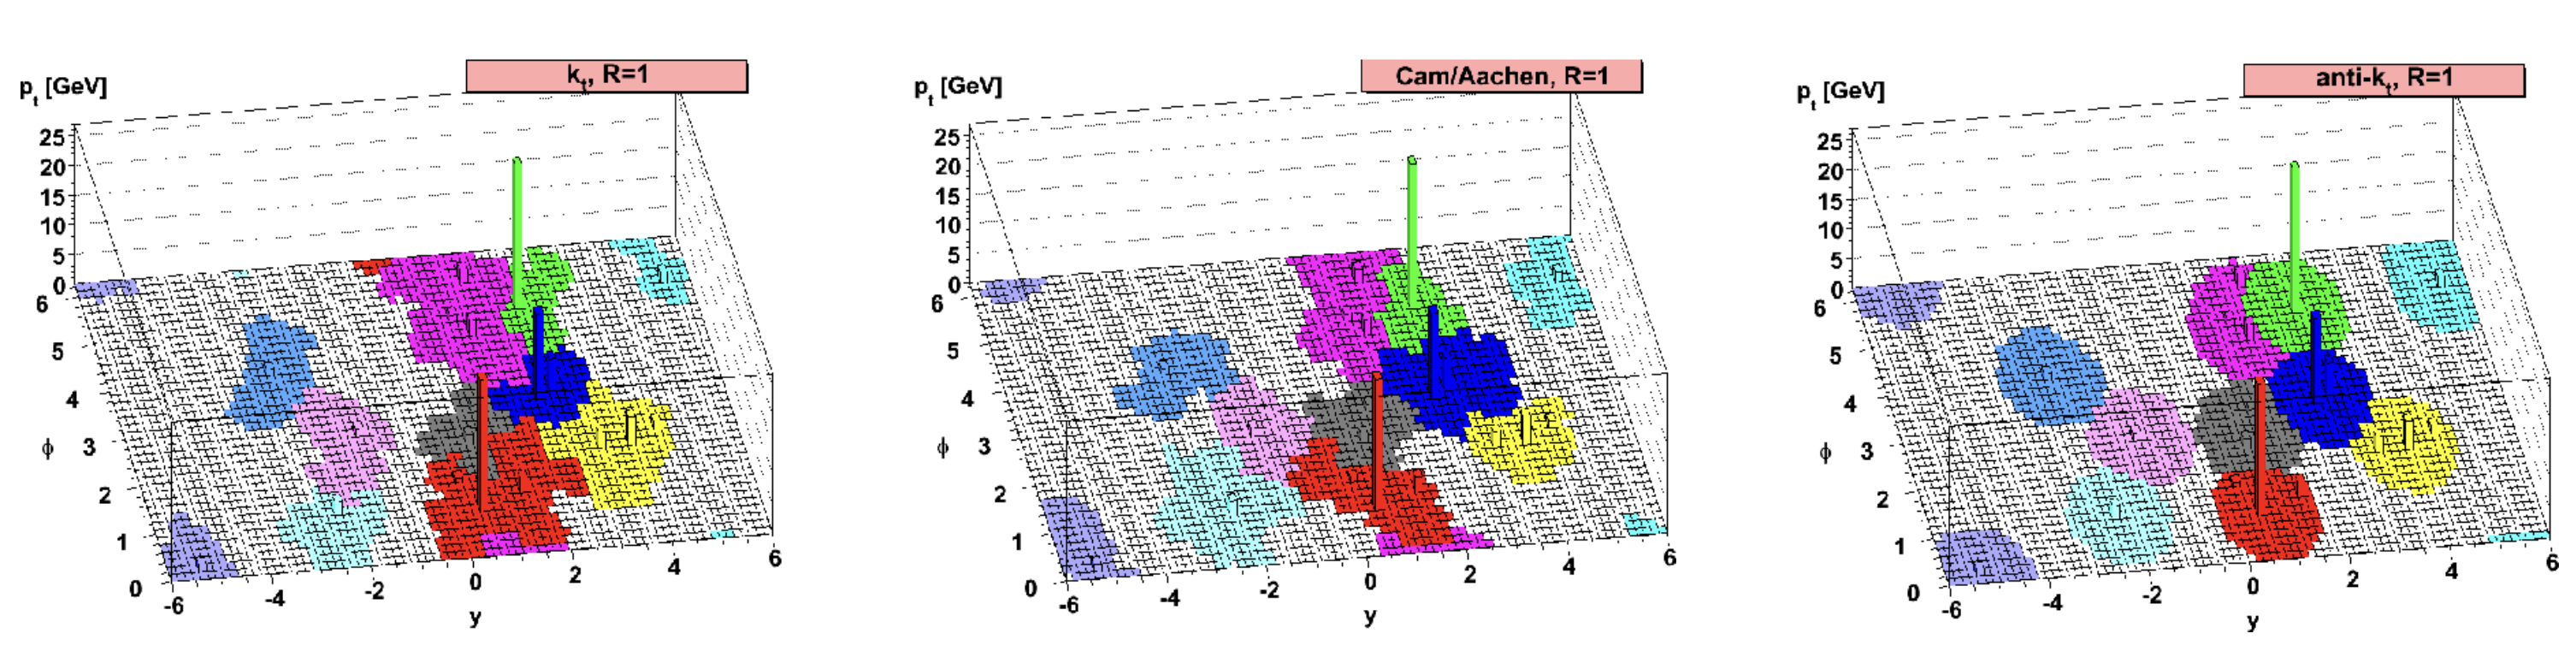
\includegraphics[width=\linewidth]{jetalgorithms.png}
	\caption{Jets reconstructed using the $k_{\rm T}$ (left), Cambridge/Aachen (middle), and anti-$k_{\rm T}$ (right) algorithms.}
	\label{fig:jetalgorithms}
\end{figure}
\subsection{SoftDrop}
The soft drop grooming procedure can be summarized as follows. First, the observed jet is reclustered with the Cambridge/Aachen (C/A) algorithm.
Second, the soft drop criterion from Eq. \ref{eq:softDropCrit} is checked at each clustering step when going backward through the C/A clustering tree.
\begin{equation}
	\label{eq:softDropCrit}
	\frac{\min(p_\mathrm{T,1}, p_\mathrm{T, 2})}{p_\mathrm{T,1} + p_\mathrm{T, 2}} > z_\mathrm{cut} \left(\frac{\Delta R_{12}}{R}\right)^\beta
\end{equation}
Here \(p_\mathrm{T, \{1,2\}}\) are the momenta of the two branches that had been merged together and \(\Delta R_{12}\) is their geometric distance in the \etaphi plane. 
%
When the softer branch fails the criterion it is removed from the jet and the procedure continues until it is satisfied. 
%
The remaining particles in the jet constitute the soft drop groomed jet. 
%
A convenient choice can be made for the soft threshold parameter \(z_\mathrm{cut}\) and the angular exponent \(\beta\). 
%
For \(\beta = 0\) the soft drop procedure reduces to the modified mass drop tagger (mMDT). 
%
Using SoftDrop, we can decompose angularities into pQCD and npQCD components. 
%
pQCD component is the angularity calculated from the jet after grooming has been performed and the npQCD component is calculated as the difference between the inclusive/ungroomed and groomed jet angularities. 

\begin{align}
	\mathcal{O}_\beta^\mathrm{\kappa} &= \mathcal{O}_\mathrm{\beta, pQCD}^\kappa + \mathcal{O}_\mathrm{\beta, npQCD}^\kappa \notag\\
	\mathcal{O}_\mathrm{\beta, pQCD}^\kappa &\equiv \mathcal{O}_\mathrm{\beta, g}^\kappa \notag \\
	\mathcal{O}_\mathrm{\beta, npQCD}^\kappa &\equiv \Delta\mathcal{O}_\mathrm{\beta}^\kappa = \mathcal{O}_\beta^\mathrm{\kappa} -  \mathcal{O}_\mathrm{\beta, g}^\kappa
\end{align}

Using the momentum balance (\(z_\mathrm{g}\)) and angularity of the first collinear-splitting (\(R_\mathrm{g}\)), we get direct connection between measurement of jet shapes and calculations from field theory. 
%
Larger \(R_\mathrm{g}\) implies that the most prominent split in the jet occurred earlier in its evolution, opening up more phase space for pQCD splittings (which survive SoftDrop grooming) because of color coherence discussed earlier.
%
Fig.~\ref{fig:GroomingAndRg} shows percentage npQCD contribution to jet width \(\left(\frac{\Delta \lambda_1^1}{\lambda_1^1} \times 100\right)\) decreasing  with increasing \(R_\mathrm{g}\), going from highly collimated, pencil-like jets to jets with proper two pronged structure.
\begin{figure}
	\label{fig:GroomingAndRg}
	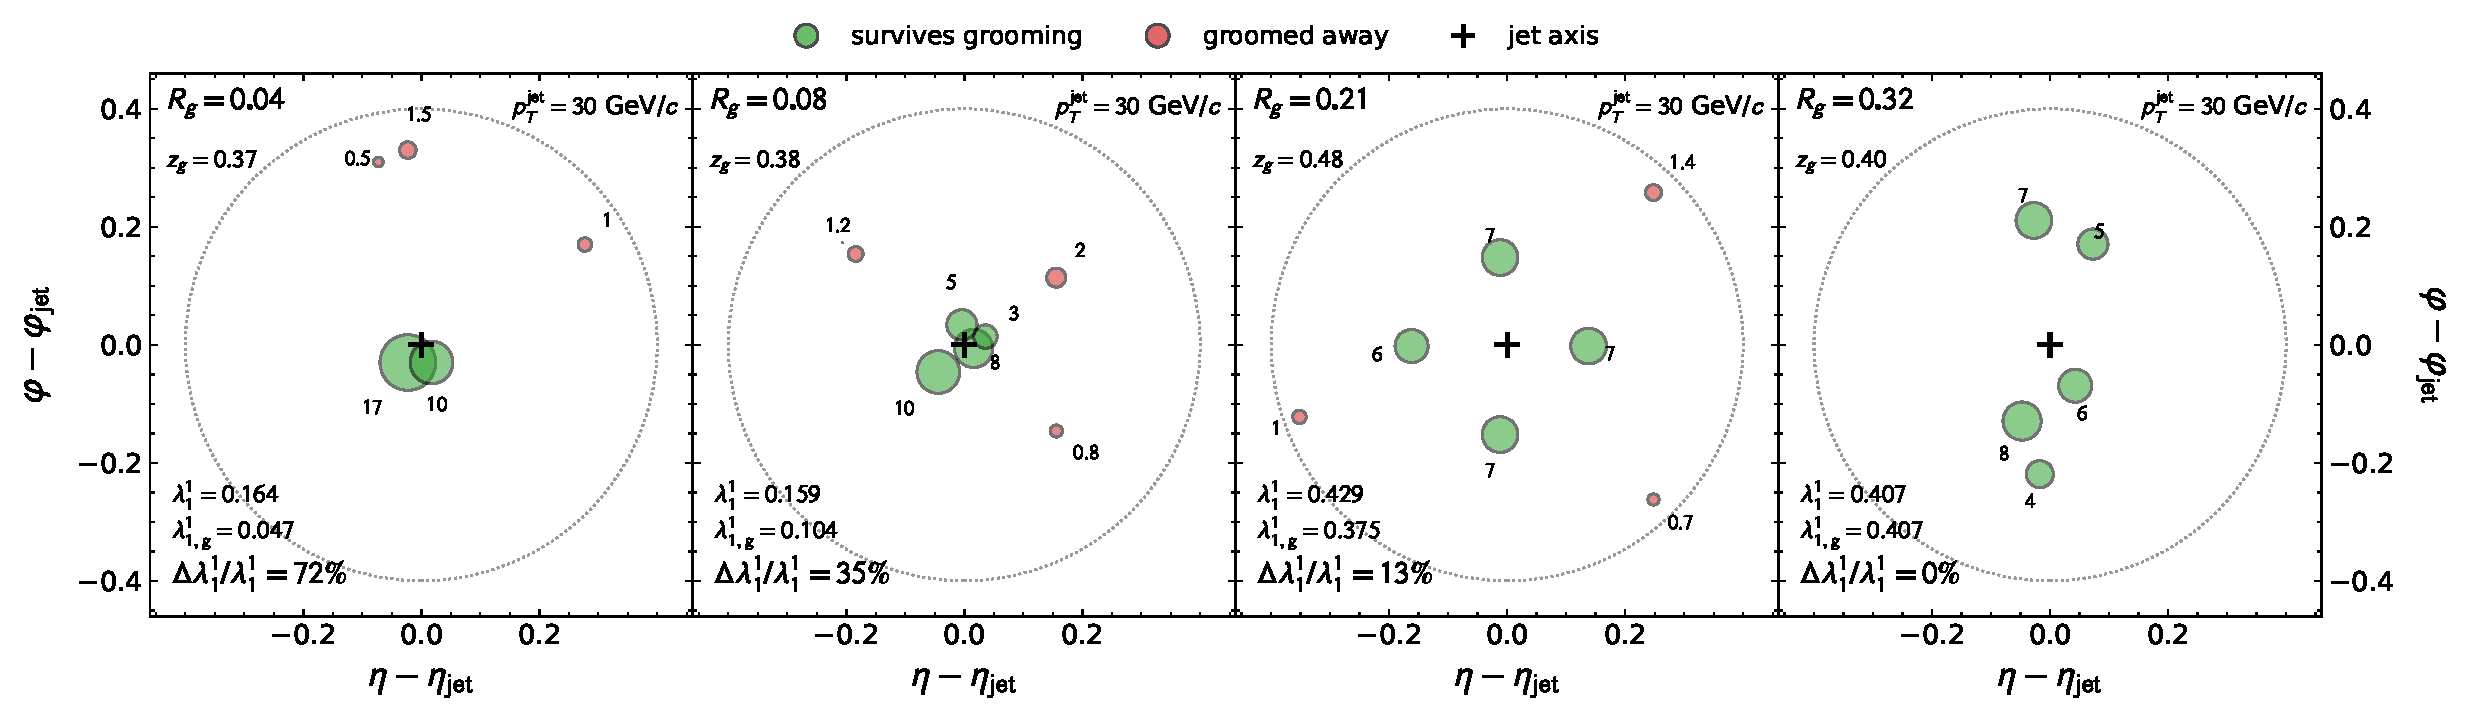
\includegraphics[width=\linewidth]{figures/fig_grooming_cartoon_4panel.pdf}
	\caption{ Ways of arranging constituents (each represented as a circle whose radius represent \(\frac{p_\mathrm{T, const}}{p_\mathrm{T, jet}}\)) in the \etaphi space within a jet with \(p_\mathrm{T, jet} = 30~\text{GeV}/c\) such that \(R_\mathrm{g}\) of the jet increases going from left to right. Green (Red) colored constituents survive (are removed by) the SoftDrop grooming ( \(z_\mathrm{cut} = 0.2,~\beta = 0\)).}
\end{figure}


\section{Heavy-Ion Collisions}
\label{sec:heavyIonCollisions}

\begin{figure}
	\centering
	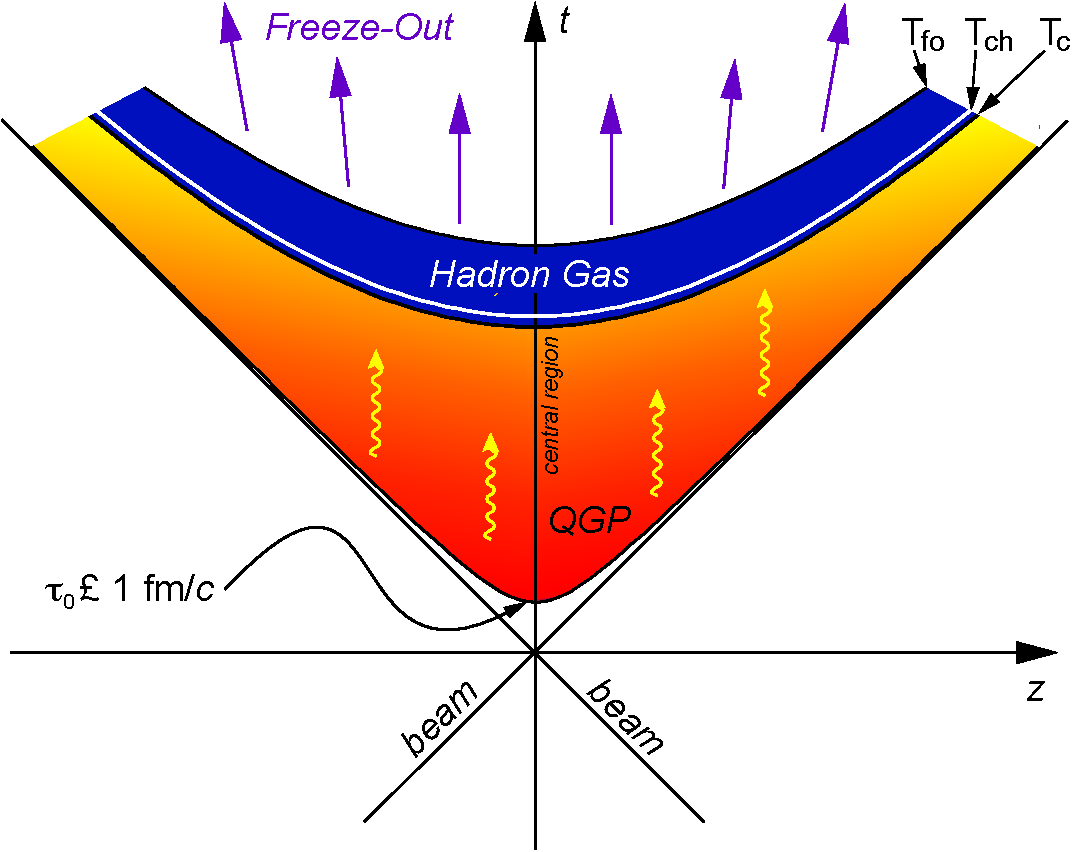
\includegraphics[width=0.7\linewidth]{figures/LightCone1_color-crop}
	\caption{A light cone diagram showing the stages of a heavy ion collision.  The abbreviation  $T_{\mathrm fo}$ is for the thermal freeze-out temperature, $T_{\mathrm ch}$ is for the chemical freeze-out temperature, and $T_{\mathrm c}$ is for the critical temperature where the phase transition between a hadron gas and a QGP occurs.  $\tau_0$ is the formation time of the QGP.}
	\label{fig:lightcone}
\end{figure}

Estimates of the energy density indicate that central heavy ion collisions with an incoming energy per nucleon pair as low as \sNN{7.7} GeV, the lower boundary of collision energies accessible at RHIC, can reach energy densities above 1 GeV/fm$^3$~\CITETHIS and that collisions at 2.76 TeV, accessible at the LHC, reach energy densities as high as 12 GeV/fm$^3$~\CITETHIS. Contrary to initial naive expectations of a gas-like QGP, the QGP formed in these collisions was shown to behave like a liquid of quarks and gluons ~\CITETHIS.

\subsection{Space-time picture of QGP}
\label{sec:qgpSpacetime}
The heavy ion collision and the evolution of the fireball, as depicted in Figure~\ref{fig:lightcone}, has several stages, and the measurement of the final state particles can be affected by one or all of these stages depending on the production mechanism and interaction time within the medium. 
%
Immediately after the collision, the system is in a non-thermalized, pre-equilibrium state where, partons undergo hard scattering, dominated by \(2\to 2\) QCD processes with the outgoing partons back-to-back in azimuth (\(\Delta \varphi \approx \pi\)). 
%
At \(\tau \approx 0.5 - 1~\text{fm}/c\), the system thermalizes into the QGP state which expands following hydrodynamic laws. 
%
During the expansion, the system cools down until it reaches the temperature (\(T_c \approx 156\)~MeV from lattice QCD studies) at which a crossover phase transition to a hadronic gas state occurs. 
%
By \(\tau \approx 10~\text{fm}/c\) after the collision for LHC energies, confinement is restored and hadronisation of quarks into colourless hadrons takes place. 
%
When the chemical freeze-out temperature (\(T_{ch} \approx 165\)~MeV) is reached, the particle abundances of the system are frozen. 
%
Elastic interactions can still occur till the kinetic freeze-out (\(T_{fo} \approx 100\)~MeV), where the particle momentum spectra are established.


%\begin{figure}[h]
%	\centering
%	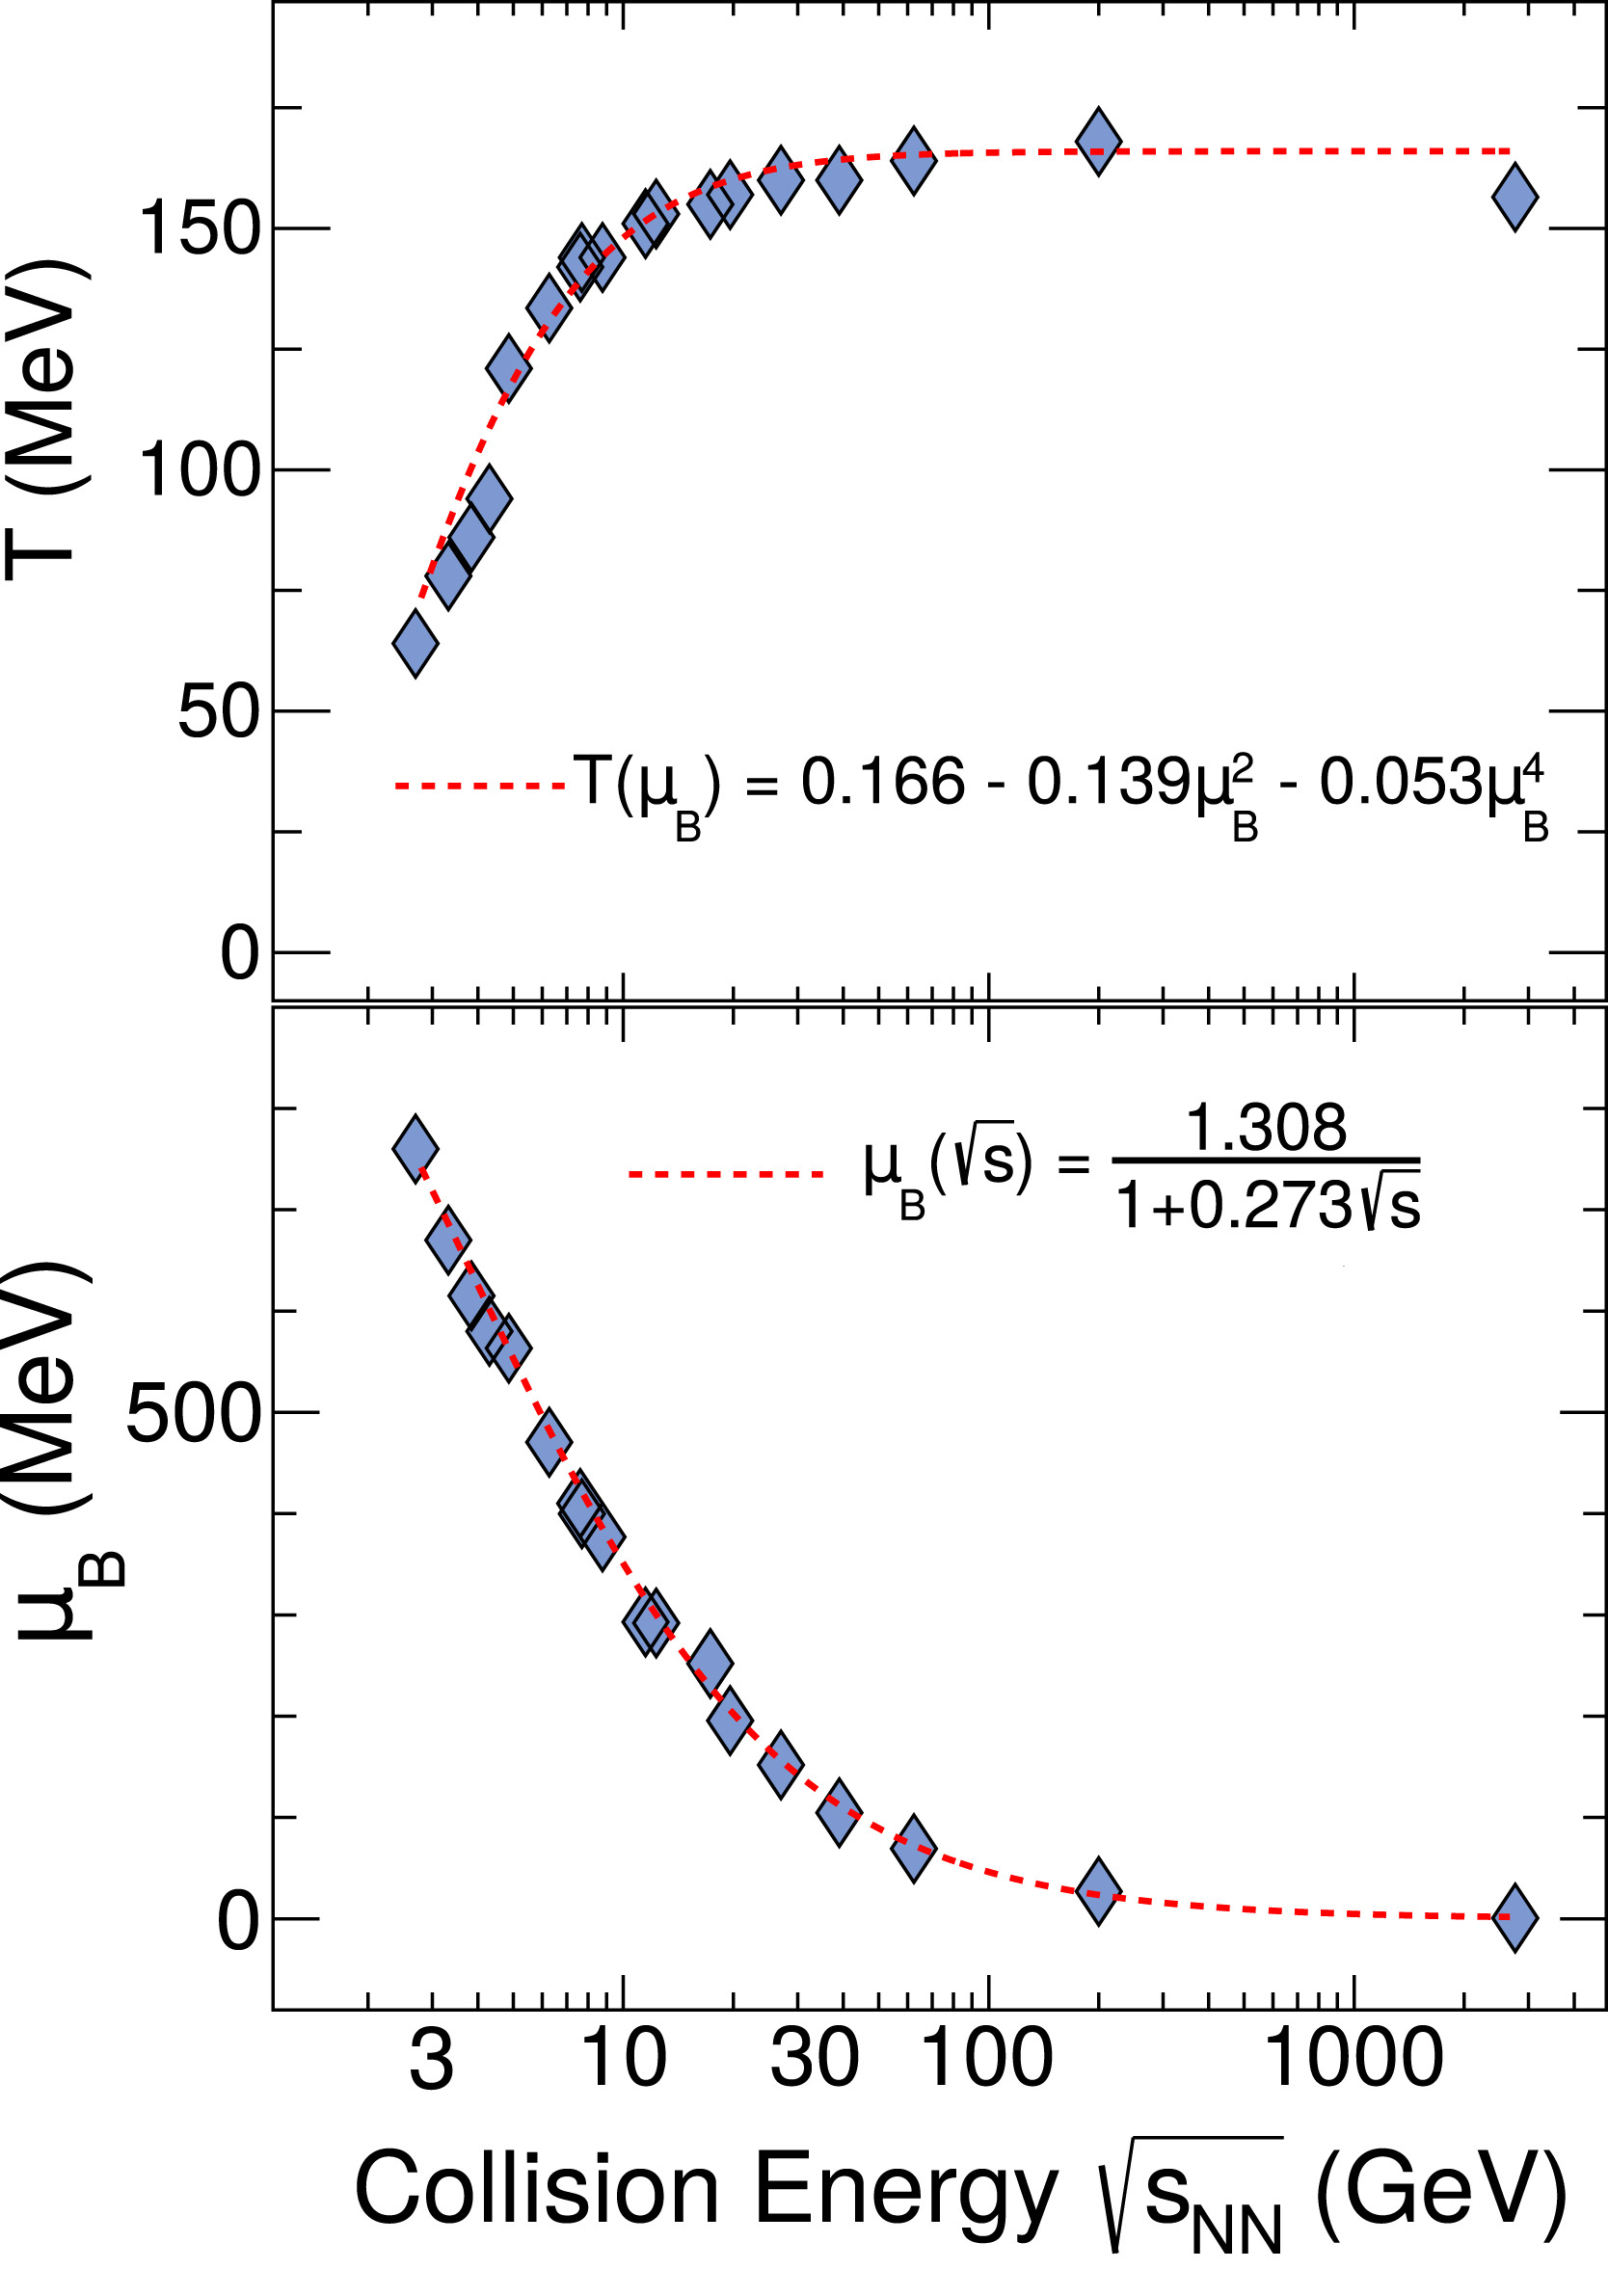
\includegraphics[width=0.5\linewidth]{figures/T_mu_vs_sNN}
%	\caption{Chemical freeze-out parameters \(T\) and \(\mu_\mathrm{B}\) obtained by thermal model fits to experimental data on particle yields as a function of collision energies. Red line represents parametrizations of \(T\) and \(\mu_\mathrm{B}\) as a function of $\sqrt{s_\mathrm{NN}}$}
%	\label{fig:tmuvssnn}
%\end{figure}
\subsection{Initial State of Colliding Nuclei}
The initial state of the incoming nuclei is not precisely known, but its properties impact the production of final state particles.  
%
The incoming nuclei are often modeled as either an independent collection of nucleons called a Glauber initial state~\CITETHIS, or a wall of coherent gluons called a Color Glass Condensate~\CITETHIS. 
%
The widely used model for determining these quantities is the Glauber Monte Carlo (Glauber MC) model, which assumes Wood–Saxon density distribution of nucleons.
%
The nuclei are then assigned a random impact parameter and translated to collide. 
%
If the distance between centers of nucleons is less than \(\sqrt{\sigma_\mathrm{inel}^\mathrm{NN}/\pi}\), where \(\sigma_\mathrm{inel}^\mathrm{NN}\) is the inelastic nucleon–nucleon cross section, the nucleons have undergone a binary collision. 
%
Nucleons that have undergone at least one binary collision are said to have participated in the reaction.
%
This procedure is followed to obtain the number of participant nucleons (\(N_\mathrm{part}\)) and the number of binary collisions (\(N_\mathrm{coll}\)) event-by-event.

A schematic diagram of the geometry of heavy-ion collisions is shown in Fig. \ref{fig:hictikz}. 
\begin{figure}
	\centering
	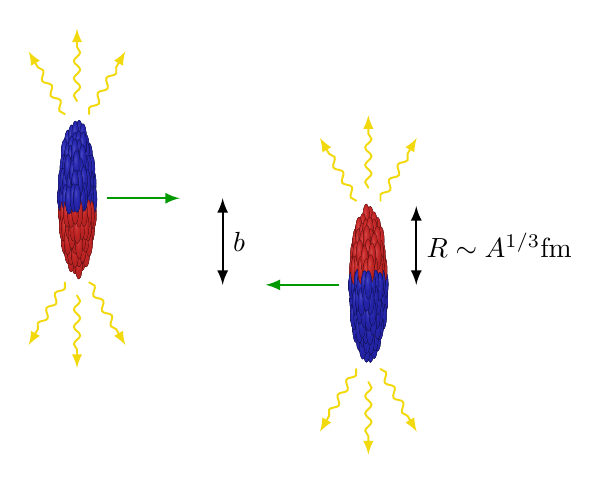
\begin{tikzpicture}
		\def\N{85} % number of nucleons
		\def\R{1.0} % nucleus radius
		\def\Nlay{5} % number of rings/layers
		\def\xs{0.25} % horizontally scale
		\def\Rp{0.92} % length photon
		\def\D{3.7} % horizontal distance between nuclei
		\pgfmathsetmacro\H{1.10*\R} % vertical distance between nuclei
		\pgfmathsetmacro\v{0.25*\D} % length vector
		
		%\message{^^J PbPb collision with impact parameter}
		
		% NUCLEUS
		% participants: nucleons in the vertical band where the two nuclei overlap
		\pic[xscale=\xs,nucleus participants,nucleus ymin=-\R,nucleus ymax=\R-\H] (L) at (-\D/2, \H/2) {nucleus};
		\pic[xscale=\xs,nucleus participants,nucleus ymin=\H-\R,nucleus ymax=\R] (R) at ( \D/2,-\H/2) {nucleus};
		
		% VELOCITY VECTORS
		\draw[vector] (L-0)++(2pt,0) --++ (\v,0); %node[above=2pt] {$v\approx c$};
		\draw[vector] (R-180)++(-2pt,0) --++ (-\v,0); %node[above=2pt] {$v\approx c$};
		
		% PHOTONS
		\foreach \ang in {60,90,120,-60,-90,-120}{
			\draw[photon] (L-\ang) --++ (\ang:\Rp);
			\draw[photon] (R-\ang) --++ (\ang:\Rp);
		}
		
		% MEASURES
		\draw[<->,thick]
		(R-0)++(0.3*\R,0) --++ (0,\R) node[midway,right] {$R\sim A^{1/3}\mathrm{fm}$};
		\draw[<->,thick]
		(0,-\H/2) -- (0,\H/2) node[midway,right] {$b$};
		%\node at (0.3*\D,0.7*\H) {$b > 2R$};
		
	\end{tikzpicture}
	\caption{Typical heavy-ion collision with an impact parameter of \(b\). The participating nuclei are colored red and the spectators are colored blue.}
	\label{fig:hictikz}
\end{figure}

\subsection{Centrality Determination} \label{sect:CentEP}
\begin{figure}[h]
	\label{fig:centralityVsNch}
	\centering
	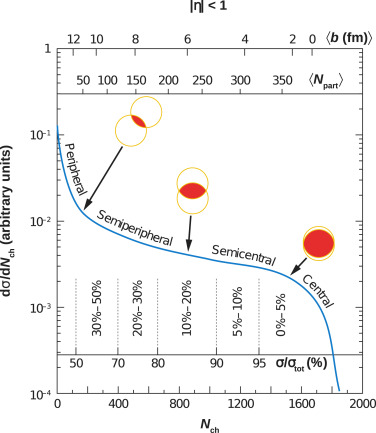
\includegraphics[width=0.6\textwidth]{figures/centrality_refmult.jpg}
	\caption{An illustration of the total inclusive charged particles multiplicity \(N_\mathrm{ch}\) and number of participant (\(N_\mathrm{part}\)) and impact parameter (\(b\)) in heavy-ion collisions}
\end{figure}
As the impact parameter  (\(b\)) of collisions, the distance between the geometrical centers of the colliding nuclei, is not measurable in experiments, a proxy called \emph{centrality} is defined. 
%
Centrality is characterized by the charged particle multiplicity of events, connected to the impact parameter through a simulation defining it as a function of \(N_\mathrm{part}\), \(N_\mathrm{coll}\) 
%
\(N_\mathrm{part}\), \(N_\mathrm{coll}\) and impact parameter \(b\) from Glauber model is mapped with the experimental data through a particle production model called the Two-Component Model\CITETHIS. 
%
Assuming that particle production is governed by contribution from hard component (\(\propto N_\mathrm{coll}\)) and soft component (proportional to  \(\propto N_\mathrm{part}\)), it simulates the multiplicity distribution according to
\begin{equation}
	N_\mathrm{ch} = n_{pp}\left[xN_\mathrm{coll} + (1-x)\frac{N_\mathrm{part}}{2}\right]
\end{equation}
where the quantity \(n_{pp}\) is the multiplicity from a \(p+p\) collision of the same center-of-mass energy. \(x\) is the contribution of hard component. 
%
\(n_{pp}\) is drawn from a negative binomial distribution with parameters \(\text{NBD }(n_{pp}; \langle n_{pp}\rangle,k)\), where \( \langle n_{pp}\rangle\) is the average multiplicity in the \(p+p\) collision and \(k\) is the width of the distribution. 
%
The simulated charged multiplicity distribution is then fitted with the corresponding multiplicity distribution from the experiment. \(\langle n_{pp}\rangle\), \(k\), and \(x\) are kept as free parameters in the fitting to experimentally measured charged particle multiplicity distribution. 
%
Initial guess values for \(x\) could be set close to those determined in different experiments for faster convergence of fitting. 

An event belongs to a centrality class, say 0\%–5\% if its charged particle multiplicity falls in the top \(5^\text{th}\) percentile. 
%
Fig.~\ref{fig:centralityVsNch} illustrates collision centrality definition in heavy-ion collisions by comparing the charge particle multiplicities with Glauber MC + Two-component model simulation.
%
Centrality classes are classified for the simulated distribution. 
%
\(\langle N_\mathrm{part}\rangle\), \(\langle N_\mathrm{coll}\rangle\) in those centrality classes are calculated. 

\subsection{Anisotropic flow}
\begin{figure}[h]
	\centering
	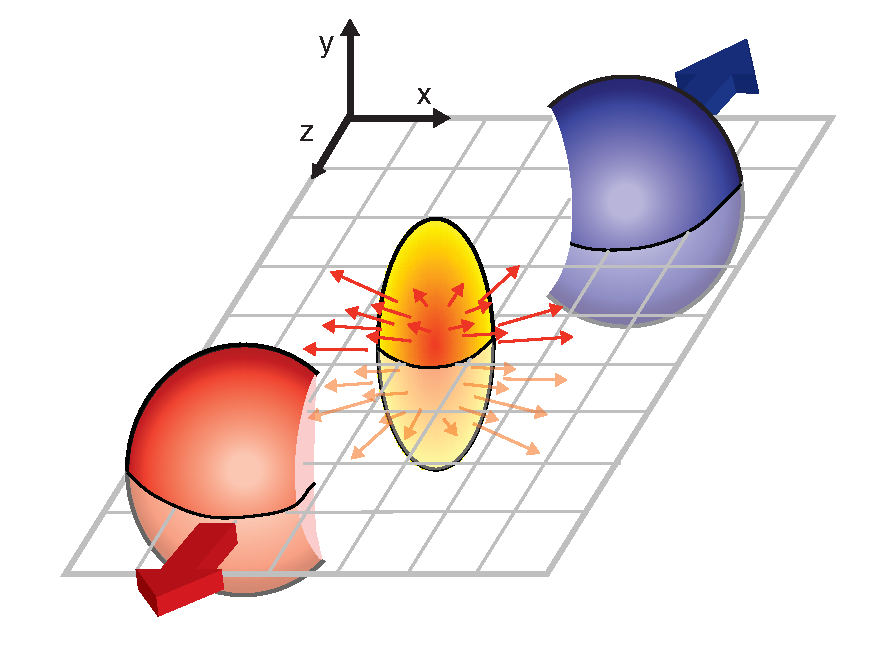
\includegraphics[width=0.4\textwidth]{figures/flow_elliptic_init_v4.pdf}
	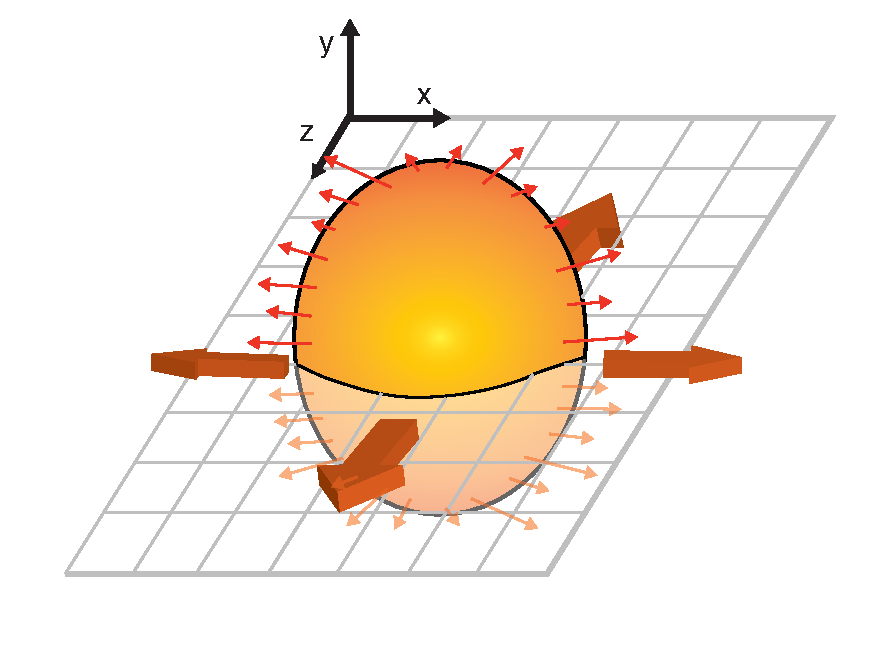
\includegraphics[width=0.4\textwidth]{figures/flow_elliptic_expd_xyz_v2.pdf}
	\label{fig:anisotropycartoon}
	\caption{Schematic diagrams showing the initial overlap region (left) and the spatial anisotropy generated by this anisotropic overlap region.  This anisotropy can be quantified using the Fourier coefficients of the momentum anisotropy.}
\end{figure}
Mean free path of particles in QGP fireball ($l$) is much smaller than the fireball's system size ($R$).
%
Hence, in non-central heavy ion collisions the initial state coordinate space asymmetry generates a pressure gradient in the direction of the impact parameter $b$, schematically shown in fig.~\ref{fig:anisotropycartoon}. 
%
This spatial asymmetry translates into a azimuthal momentum anisotropy as the system expands, meaning that particles are more likely to be emitted along the plane where the pressure gradients are the highest. 
%
This plane is defined by the beam axis and the impact parameter of the collision, and called the \emph{reaction plane} (\(\Psi_{\rm RP}\)).
%
The anisotropy can be characterized by the Fourier decomposition of the azimuthal particle distribution with respect to \(\Psi_{\rm RP}\)~\cite{Bielcikova:2003ku,Voloshin:1994mz}:
\begin{equation}
	\frac{dN}{d(\phi - \Psi_{RP})} = \frac{N_0}{2\pi} \left( 1 + 2 \sum_{n=1}^{\infty} v_n \cos[n(\phi - \Psi_{RP})] \right),
	\label{fourier_azi_part_distr}
\end{equation}
%
The \emph{anisotropic flow} coefficients $v_{n}$, the $n^{\rm th}$ order term in the Fourier decomposition of the final state particle azimuthal distribution is given by,
%
\begin{equation}
	\label{flow}
	v_{n} = \left< \cos([n(\phi - \Psi_{\rm RP})]) \right>
\end{equation}
%
Due to the symmetry of the collision geometry, the most prominent contribution is from the second order coefficient $v_2$, called \emph{elliptic flow}.

\begin{figure}[h]
	\centering
	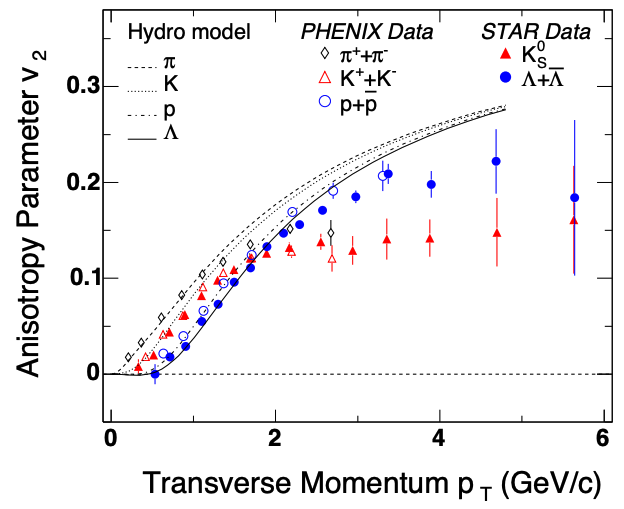
\includegraphics[width=0.41\linewidth]{AnisotropyWithNoScaling (1).png}
	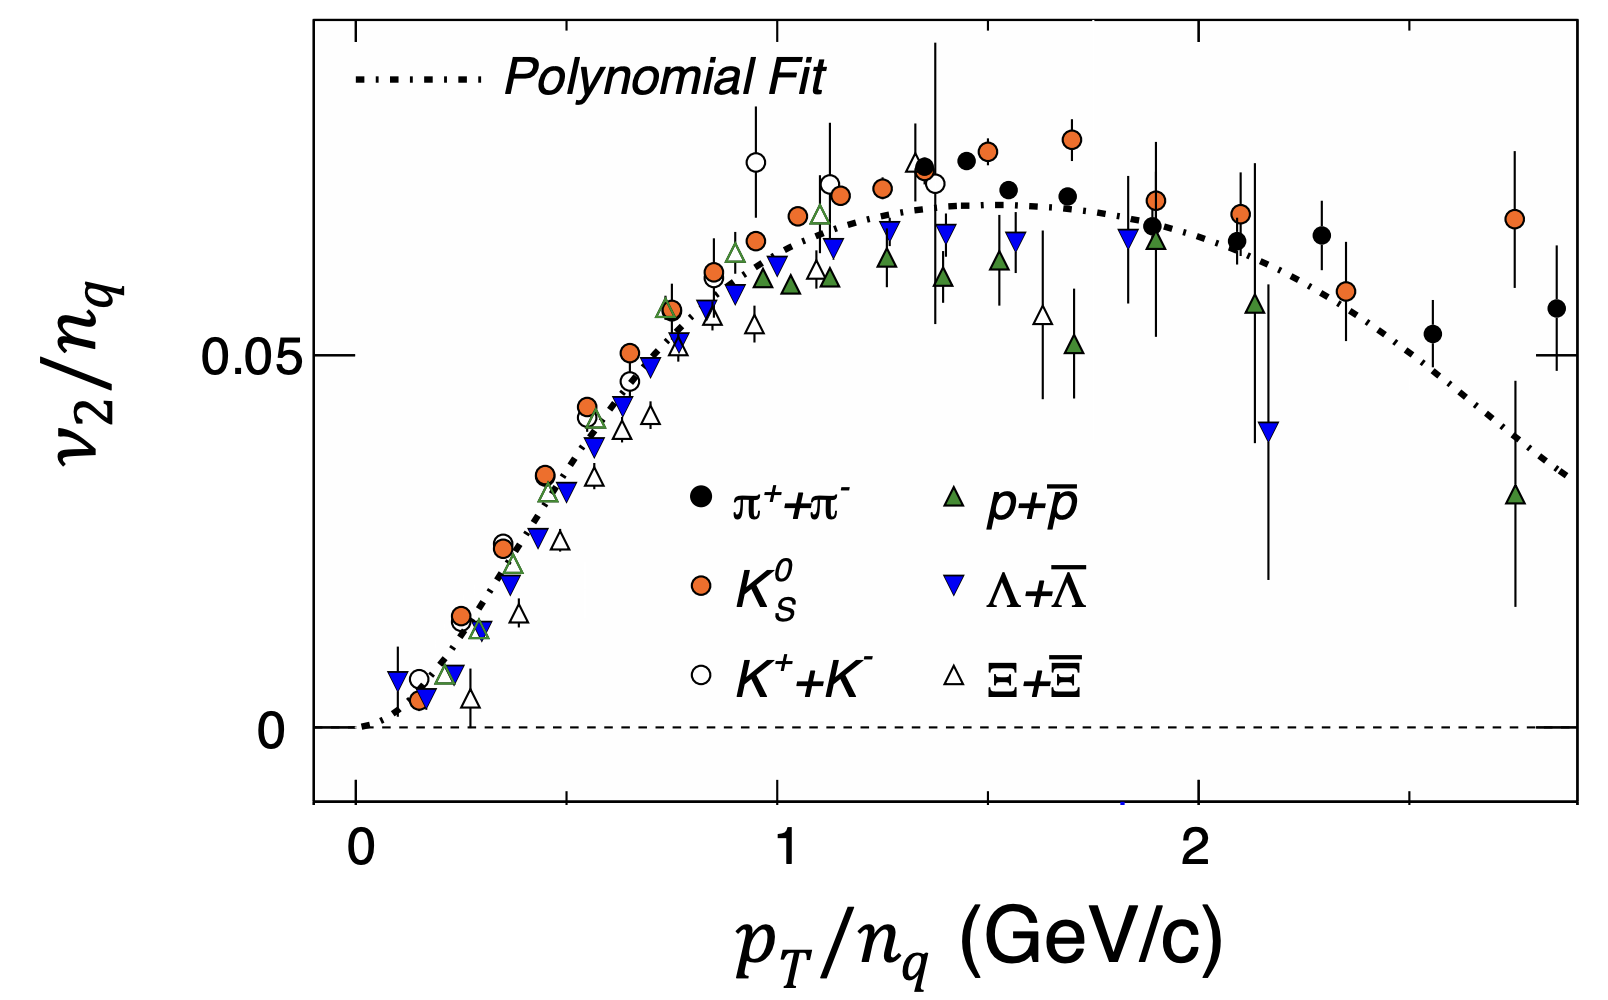
\includegraphics[width=0.52\linewidth]{Gen1_IdentifiedParticle_v2.png}
	\caption{\textbf{Left panel}: Elliptic flow $v_2$ for several particle species in Au + Au collisions at \sNN{200}{GeV}  from STAR and PHENIX experiments. Predictions from hydrodynamic models are shown as lines. Taken from \cite{GYULASSY200530}. \textbf{Right panel}: Number of constituent quarks ($n_q$) scaled $v_2$ as a function of $p_{\rm T}/n_q$. Taken from \cite{Sorensen_2006}.}
	\label{fig:AnisotropyResults}
\end{figure}

$v_2$ was measured by the STAR and PHENIX for several particle species and is shown in Fig. \ref{fig:AnisotropyResults}. 
%
Large positive $v_2$ values indicate collective phenomena associated with a strongly coupled fluid, or a \emph{signature of QGP}.
%
A scaling of the $v_2$ values with the number of constituent quarks (2 for mesons, 3 for baryons) yielded a universal curve as a function of $p_{\rm T}/n_q$ suggesting the flow dynamics were developed in a medium with quark and gluon degrees of freedom, i.e. QGP.

\subsubsection{Event plane reconstruction}
\label{sec:EP_Recon}
The reaction plane, \(\Psi_{\rm RP}\) cannot be directly measured and is approximated by the second-order symmetry plane, $\Psi_{2,EP}$, referred to as the \emph{event plane}  in this text, for simplicity.  
%
\(\Psi_{\rm RP} \to \Psi_{2, EP}\) if nucleon distributions were in their average positions and devoid of fluctuations from interactions among nucleons~\cite{PhysRevC.101.064901}.
%
By measuring the charged particle azimuthal distribution, the n-th order event plane can be extracted by~\cite{Poskanzer:1998yz},  
%
\begin{equation}
	\Psi_{n,EP} = \frac{1}{n} \arctan \left(\frac{Q_{y, n}}{Q_{x, n}} \right),
	\label{eqn:EP}
\end{equation}
%
the weighted vector \(\mathbf{Q}_n = Q_{x, n}\hat{\mathbf{x}}+ Q_{y, n}\hat{\mathbf{y}}\) are given by,
%
\begin{align}
	\mathbf{Q}_n = \hat{\mathbf{x}}\sum_{\mathrm{tracks}} p_{\rm T, track} \cos (n \phi_{\rm track}) + \hat{\mathbf{y}}\sum_{\mathrm{tracks}} p_{\rm T, track} \sin (n \phi_{\rm track}).
	\label{Eqn:Qvecs}
\end{align}
%
where the sum is calculated for all reconstructed charged particles (tracks) in the event, $\phi_{\rm track}$ is the track's azimuthal angle, and $p_{\rm T, track}$ the track's transverse momentum.  
%

Due to finite acceptance and multiplicities, the calculated event plane has an underlying anisotropy that is corrected by applying two separate correction methods.  
%
First, a calibration and recentering correction procedures are applied to remove bias introduced by non-uniform acceptance of the TPC tracking system and further account for potential beam-condition effects~\cite{Barrette:1997pt,PhysRevC.55.1420,Poskanzer:1998yz}.  
%
This procedure involves recentering the weighted $\mathbf{Q}_2$-vectors such that, $\langle\mathbf{Q}_2 \rangle = \mathbf{0}$. 
%
It is done by calculating a modified $\mathbf{Q}_2$, obtained by subtracting an event averaged $\langle\mathbf{Q}_2 \rangle$ from each event's nominal $\mathbf{Q}_2$.
%

The higher harmonics of $\Psi_{n,EP}$ still persist after recentering \cite{Poskanzer:1998yz}, and are removed through a second correction step, referred to as  the shifting method, applied event-by-event  to make the event-plane angle isotropic in the lab frame \cite{Voloshin:2008dg}. 
%
This method defines a new angle:
%
\begin{equation}
	\Psi'_{2,EP} = \Psi_{2,EP} + \sum_n \frac{2}{n}
	(- \langle \sin (n\Psi_{2,EP}) \rangle \cos(n\Psi_{2,EP}) + \langle \cos(n\Psi_{2,EP}) \sin(n\Psi_{2,EP}) \rangle) ,
	\label{eqn:Shift}
\end{equation}
%
Usually 20 orders of Fourier moment are removed. 
%
Additional details of the recentering and shifting corrections can be found in Refs.~\cite{Wang:2012bga,Barrette:1997pt,Poskanzer:1998yz}

 The difference between $\Psi_{RP}$ and \(\Psi_{2, EP}\) is quantified by event-plane resolution, $R_n$ or $R_n\{\Psi_{2, EP}\}$ given by Eqn.~\ref{resolution}. 
 %
 The observed $v_n$, $v_n^{\rm obs}$ is corrected for this limited resolution by doing, $v_n = v_{n}^{\rm obs}/R_n$ \cite{Abbas:2013taa,Poskanzer:1998yz}.  
 %
\begin{equation}
	R_n = R_n\{\Psi_{2, EP}\} = \langle \cos(n[\Psi_{RP} - \Psi_{2, EP}]) \rangle \qquad \text{$n$ is even}
	\label{resolution}
\end{equation}

Furthermore, individual events are divided into two random sub-events by assigning charged tracks to sub-events, ``$a$" and ``$b$". 
%
The sub-events are unique, with approximately equal multiplicities. 
%
We can write the correlation of two event planes by taking the product of two sub-events, \cite{Barrette:1996rs,Poskanzer:1998yz}
%
\begin{equation}
	\langle \cos(n[\Psi_{2, EP}^{a} - \Psi_{2, EP}^{b}]) \rangle = 
	\langle \cos(n[\Psi_{2, EP}^{a} - \Psi_{RP}]) \rangle
	\langle \cos(n[\Psi_{2, EP}^{b} - \Psi_{RP}]) \rangle,
	\label{resolution2sub}
\end{equation}
%
This allows calculation of the event-plane resolution directly from data. Since $a$ and $b$ have equal multiplicities, the resolution of each sub-event can be calculated from the correlation between the two sub-events as \cite{Poskanzer:1998yz}:

\begin{equation}
	\langle \cos(n[\Psi_{2, EP}^{a} - \Psi_{RP}]) \rangle = 
	\sqrt{\langle \cos(n[\Psi_{2, EP}^{a} - \Psi_{2, EP}^{b}]) \rangle} .
	\label{resolutionIndiv}
\end{equation}

The event-plane resolution is multiplicity dependent and calculated for separate ranges of collision centrality using the two sub-events method.  
%
Narrower bins are calculated and then combined accordingly to match the ranges required, by averaging the results from the narrow bins weighted by the multiplicity of each bin \cite{Voloshin:2008dg}.

\section{Jets in QGP}
As discussed in sec.~\ref{sec:qgpSpacetime}, hard scattered partons that produce jets are produced before the system thermalizes into QGP. 
%
Thus the ensuing parton shower traverses the QGP, and resulting jet is \emph{quenched} compared to an appropriate \emph{baseline}. 
%
The two main mechanisms for jet quenching are \emph{collisional} and \emph{radiative} energy losses. 
%
Collisional energy loss happens due to the elastic scattering between the parton and the medium constituents and usually dominates for lower energy partons. 
%
Radiative energy loss happens due to induced gluon radiation (\textit{bremsstrahlung}) through inelastic scatterings with the medium particles \cite{MAJUMDER201141,QinWang2024,Burkeetal}. 
%
For partons with \ptGeq{parton}{5} , this is usually the dominant source of energy loss \cite{LandoltBornstein2010:sm_lbs_978-3-642-01539-7_16}. 
%

The baseline measurement is done in a collision system where either QGP is not formed or has negligible lifetime compared to central heavy-ion collisions. 
%
Two possible choices arise for the baseline, first is \(p+p\) collisions from which we can calculate the \emph{Nuclear Modification Factor} (\RAA) for distributions of any observable \(\mathbf{O}\) calculated in \(p+p\) and \(A+A\) collisions,
given by
\begin{equation}
	R_{\rm AA}(\mathbf{O}, b) = \frac{dN_{\rm AA}/d\mathbf{O}}{\left<T_{\rm AA}(b)\right> . d^2\sigma_{pp}/d\mathbf{O}}
\end{equation}\label{RAA}
where $T_{\rm AA}(b) = N_{\rm coll}(b)/\sigma_{\rm NN}^{\rm inel}$ is the nuclear overlap function of impact parameter (\textit{b}) \cite{doi:10.1142/S0217751X95001467}.
%
The second common baseline used in absence of a \(p+p\) baseline is peripheral collisions of heavy-ion collisions. The \emph{Relative Nuclear Modification Factor} \(R_{CP}\) is given by,
%
\begin{equation}
	R_{CP}(\mathbf{O}, b) = \frac{dN/d\mathbf{O}}{\left< N_{\rm bin}(b) \right>} \biggm\lvert_{\rm cent} \times \frac{\left< N_{\rm bin}(b) \right>}{dN/d\mathbf{O}} \biggm\lvert_{\rm peri}
\end{equation}

\begin{figure}
	\centering
	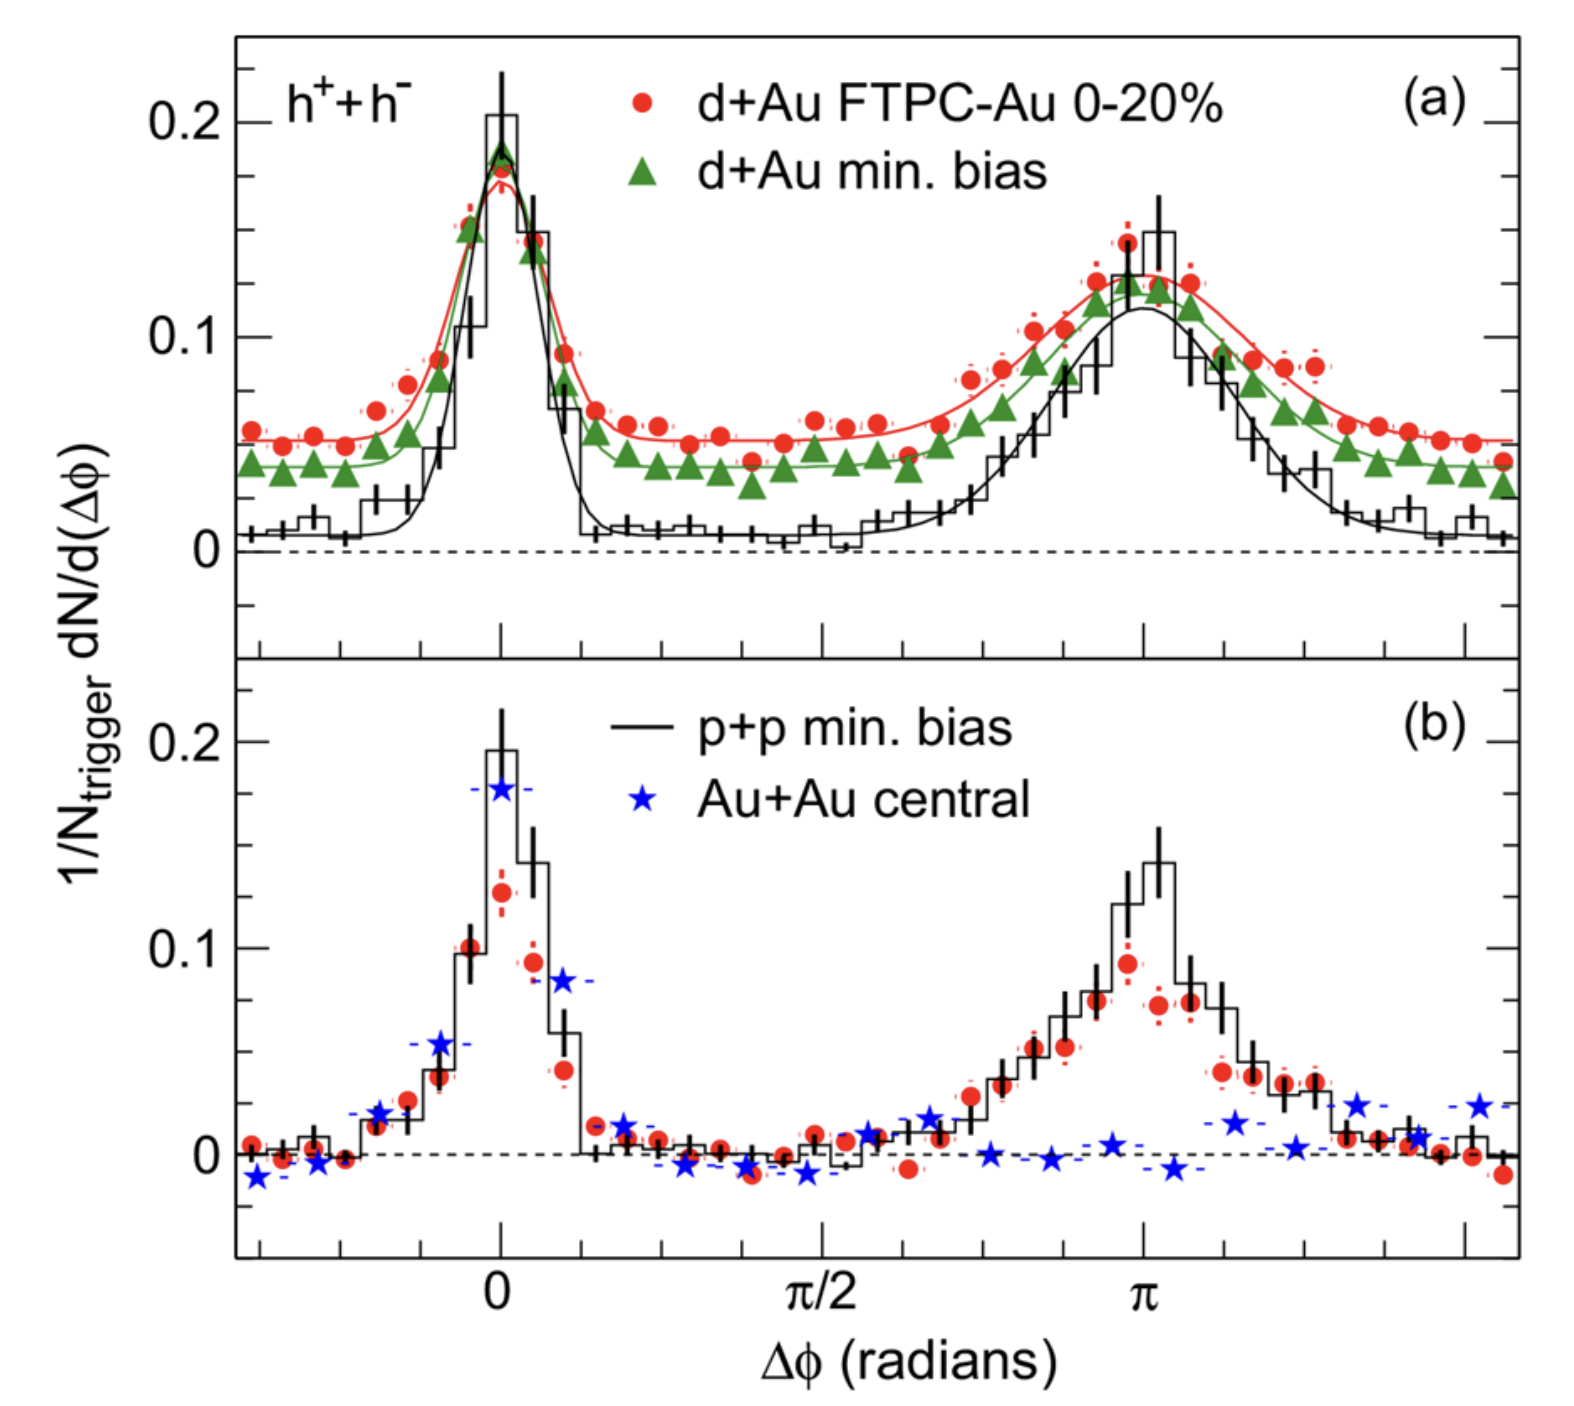
\includegraphics[width=0.8\linewidth]{Gen0_AngularCorrelation_JetQuenching.png}
	\caption{Measurement of the angular correlation between all charged hadrons and the leading hadron in the event for p + p (black lines), d + Au (red and green markers), and Au + Au events (blue markers), performed by the STAR experiment. The vanishing of the away-side yield around $\Delta\phi\approx \pi$ in Au + Au events is evidence of particles getting quenched in the QGP medium. Taken from \cite{PhysRevLett.91.072304}.}
	\label{fig:angularcorr}
\end{figure}

Before infrastructure became available to reliably reconstruct a sufficient number of jets in heavy-ion collisions,  the effects of the medium on high energy partons were studying the \emph{Di-hadron correlation}. 
%
Leading hadron (highest $p_\mathrm{T}$ in event) is used as a jet proxy and the azimuthal angular correlation ($\Delta\varphi$) of all charged hadrons in the event is studied.
%
Fig. \ref{fig:angularcorr} shows one of the first measurements performed by STAR\cite{PhysRevLett.91.072304}, di-hadron correlations compared between p + p, Au + Au, and d + Au collisions. 
%
The p + p and d + Au both show peaks around $\Delta\varphi = 0$ and $\Delta\varphi =  \pi$ as expected, given that hard scatterings are dominated by \(2\to 2\) Feynman diagrams. 
%
However, for Au + Au collisions, the peak around $\Delta\varphi = \pi$ completely vanishes. 
%
This was the expectation because depending on the distance from the center of the collision where the initial back-to-back partons were produced, one of the partons would travel a larger distance in the QGP medium and therefore lose more energy than the other one.
 
\begin{figure}
	\centering
	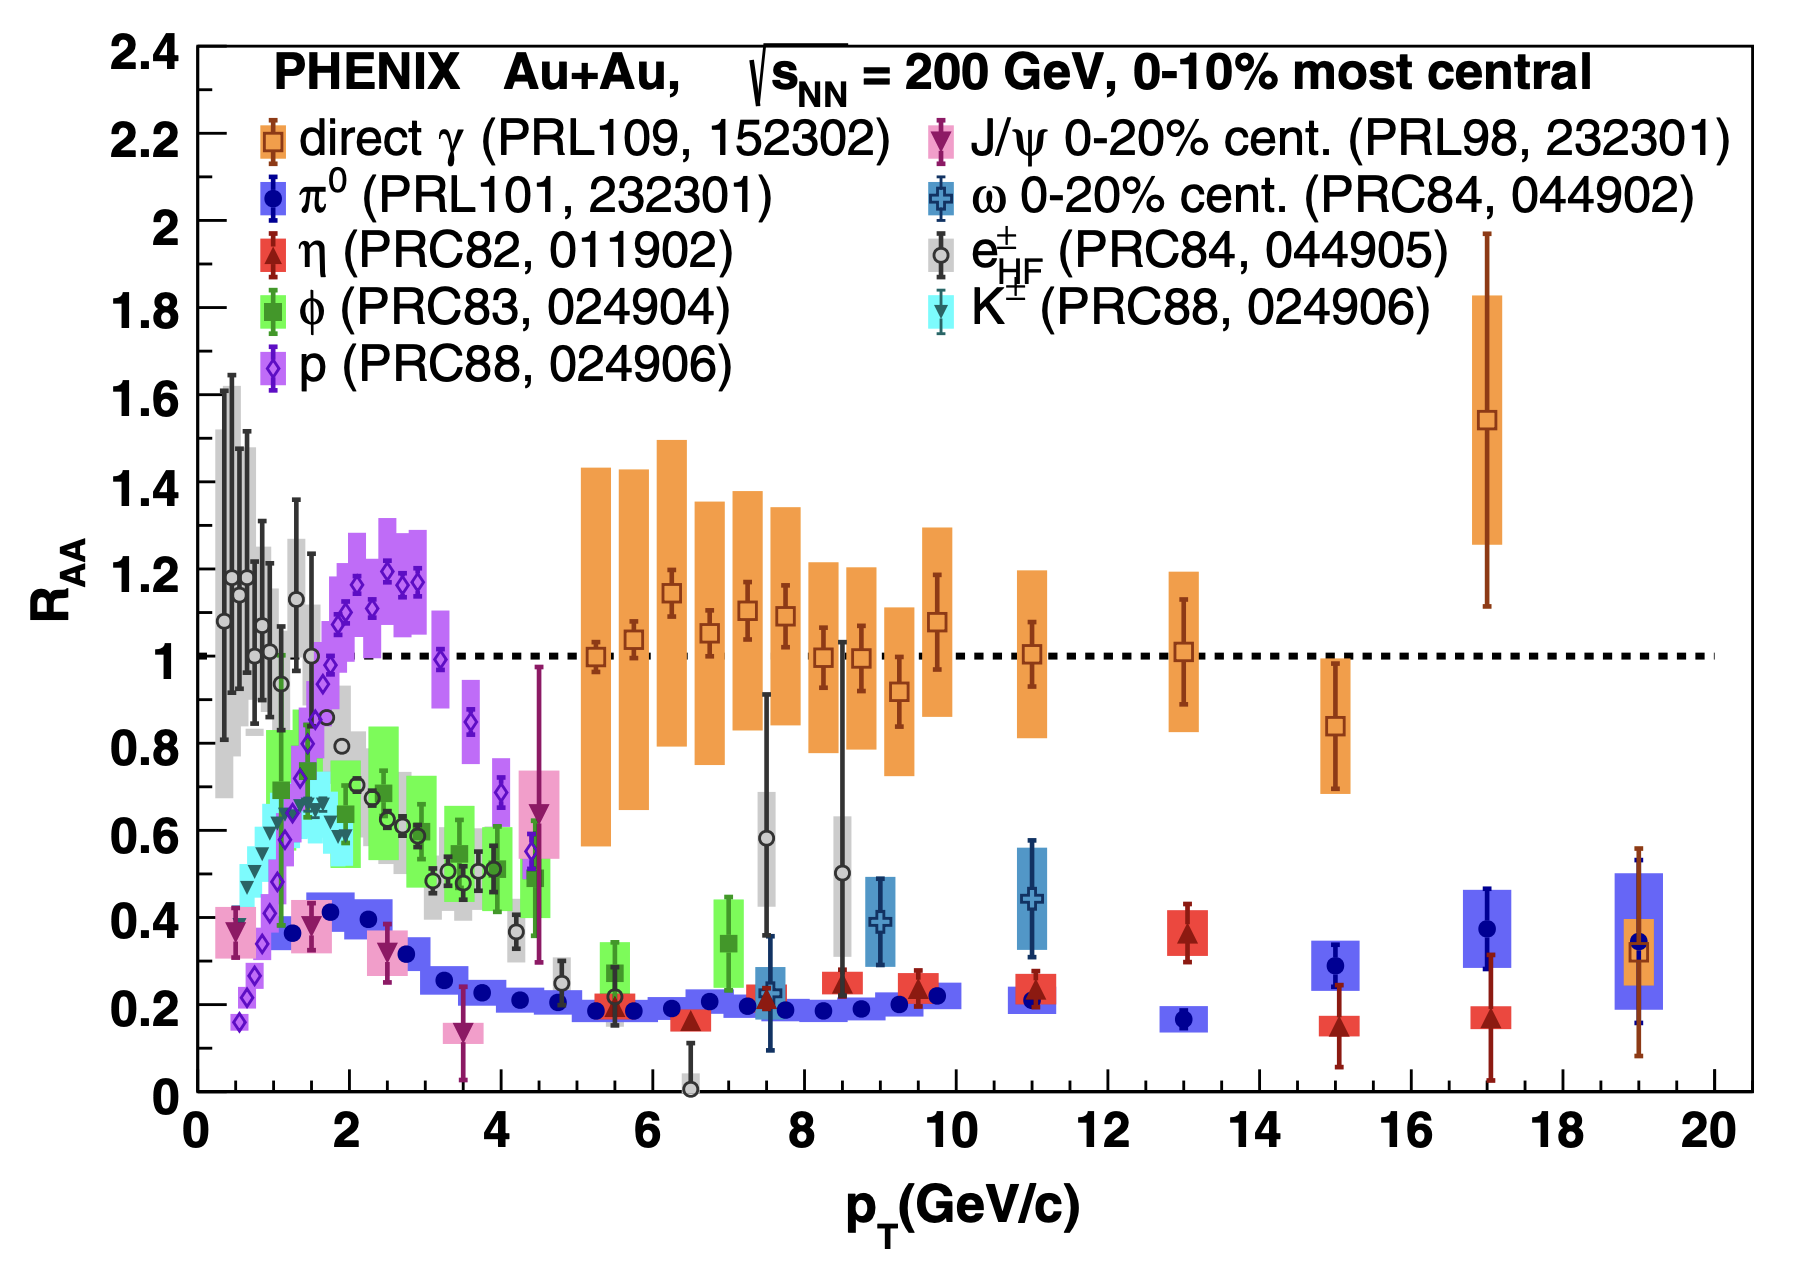
\includegraphics[width=0.8\linewidth]{Gen0_SingleParticle_RAA.png}
	\caption{Nuclear modification factor $R_{\rm AA}$ as a function of $p_\mathrm{T}$ for identified particle species in Au + Au collisions at \sNN{200}{GeV} measured by the PHENIX experiment. Taken from \cite{Tannenbaum_2015}.}
	\label{fig:singleparticleraa}
\end{figure}

A closer look at jet quenching was given by the PHENIX experiment through a collection of  \RAA measurements Eq.~\ref{RAA} for identified particles spectra, shown in Fig. \ref{fig:singleparticleraa}.
% 
All strongly interacting particles show varying levels of suppression from 0.2 - 0.6, again confirming their energy loss in the presence of QGP.

Although measurements with high $p_\mathrm{T}$ hadrons help us understand jet quenching mechanisms in the medium, they suffer from survival bias, as these hadrons arise from a subsample of jets which usually undergo the least amount of quenching \cite{PhysRevC.99.051901}. 
%
Fully reconstructed jets, however, are mostly unbiased probes of energy flow at high $p_\mathrm{T}$, and offer a wealth of substructure observables which allow us to look at energy flow within the jet more differentially.
%
This motivates the studies presented in chapters~\ref{ch:jhcorr} and~\ref{ch:angularities}.   

\begin{figure}
	\centering
	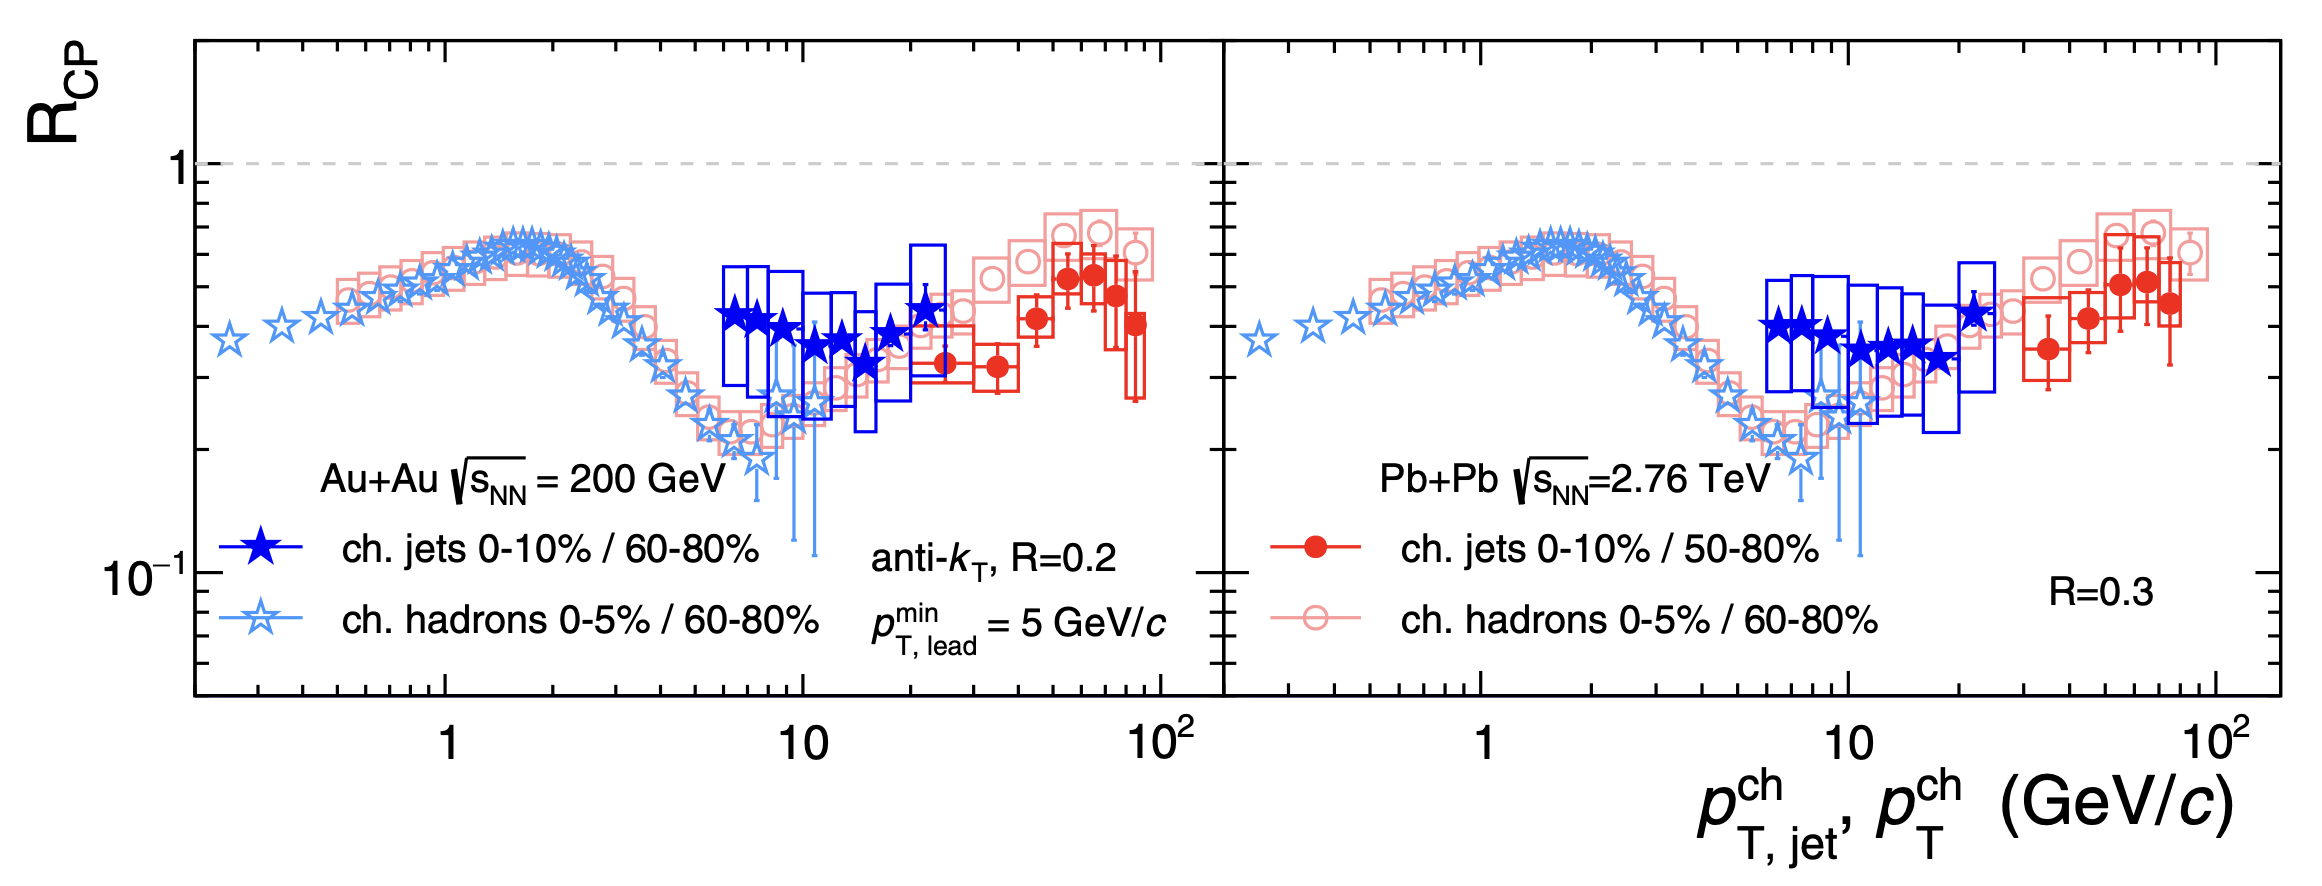
\includegraphics[width=1\linewidth]{Gen1_ChargedParticleAndJets_RCP.png}
	\caption{$R_{CP}$ distributions for charged hadrons (open markers) and jets (solid markers) from RHIC (blue star markers) and LHC (red circle markers) experiments. Taken from \cite{STARChargedJet} and references within \cite{PhysRevLett.91.172302, ALICEChargedJet, ATLASChargedHadron}.}
	\label{fig:chargedparticlercp}
\end{figure}
The STAR experiment measured the \(R_{CP}\) of the $p_\mathrm{T}$ spectra of charged particle jets (clustered charged tracks only and contain no calorimeter hits (towers) as input) from central and peripheral Au + Au collisions at \sNN{200}{GeV} shown in fig.~\ref{fig:chargedparticlercp} \cite{STARChargedJet}. 
%
Measured for charged jets was compared to $R_{CP}$ for charged hadrons from STAR at the same energy, and to the measured $R_{CP}$ for charged hadrons and jets from the ALICE and ATLAS experiments at \sNN{2.76}{TeV}. 
%
First, the charged hadrons $R_{CP}$ is found to be the same over the same range of $p_\mathrm{T}$ at RHIC and LHC energies (which are an order of magnitude apart). 
%
The charged jet $R_{CP}$ is also found to have similar values between RHIC and LHC energies with roughly 60\% of the energy lost outside the jet cone in central collisions with respect to peripheral collisions, with no significant $p_\mathrm{T}$ dependence in contrast to the $p_\mathrm{T}$ dependence observed for the charged hadrons $R_{CP}$. 
%
This may be because the inclusive hadron distribution usually arises from the leading hadron in the corresponding jet, and is therefore is sensitive to the fragmentation function. 
%
This fragmentation process can therefore introduce the $p_\mathrm{T}$ dependence of $R_{CP}$ in hadrons. 


%\chapter{Data analysis techniques}
\label{ch:methods}

As a result of the quantum-mechanical nature of the collisions and the interaction of their products with the detectors, the observations resulting from a particular interaction are fundamentally probabilistic. 
%
Therefore, the approach to data analysis and the conclusions drawn from the data must be framed in statistical terms, which include not only low-level tasks, such as the reconstruction and identification of particles and the measurement of their energies and momenta, but also high-level tasks, such as searches for new particles and measurements.
%
The high dimensionality and large volume of LHC data pose a problem because the statistical model over the high-dimensional space of their experimental data is not known explicitly in terms of an equation that can be evaluated. 
%
Instead, one typically has access to large samples of simulated data generated by stochastic simulation programs that model the physics of particle interactions on various scales. 
%
If the data were fairly low dimensional (d< 5), the problem of estimating the unknown statistical model from the simulated samples would not be difficult.
%
Histograms or kernel-based density estimates provide reasonable estimates in low-dimensional spaces. 
%
These strategies, however, suffer from the curse of dimensionality. 
%
In a single dimension, \(N\) samples may be required to describe the source probability density function. 
%
In \(d\) dimensions, the number of samples required increases to the power of the data’s dimensionality: \(\mathcal{O}(N^d)\). 
%
The consequence is that any dimensionality greater than five or ten requires impractical or impossible computational resources, regardless of the speed of the sample generator.

%In parallel to the relatively recent rise of ML techniques in industrial applications, scientists have increasingly become interested in the potential of ML for fundamental research, and HEP is no exception.
%
%Traditionally, HEP physicists have approached this problem by reducing the dimensionality of the data through a series of steps that operate both on individual collision events and on collections of events. For an individual event, reconstruction algorithms process the raw sensor data into low-level objects such as calorimeter clusters and tracks. 
%%
%From these low-level components, the algorithms attempt to estimate the energy, momentum, and identity of individual particles.
%% 
%Next, from these reconstructed objects, event-level summaries are constructed. 
%%
%Event selection algorithms then select subsets of the collision data for further analysis on the basis of the information associated with individual events. 
%%
%Traditionally, the reconstruction and event selection operations are based on specific, engineered features in the data. 
\section{Machine Learning Basics}
Fortunately, many of the tasks encountered in HEP can be naturally reformulated as machine learning problems. 
%
Typically, the problems are formulated in terms of a search for some function \(f:X \to Y\), from the space of the observed data \(X\) to a low-dimensional space of a desired target label \(Y\), which optimizes some metric of our choosing. 
%
This metric is called a loss function and is written as \(L[ \mathbf{y}, f (\mathbf{x})]\).
%

Ideally, a learning algorithm would find the function that optimizes \(L\) over all possible values
of \((\mathbf{x}, \mathbf{y})\), but this is intractable owing to the curse of dimensionality and an infinite number of functions to choose from. 
%
Instead, in supervised learning, one has labeled training data \(\{\mathbf{x}_i , \mathbf{y}_i\}^N_{i=1}\) sampled from \(p(\mathbf{x} , \mathbf{y})\). 
%
Furthermore, the function space is restricted to a model—a highly flexible family of functions \(f_\phi(\mathbf{x})\) parameterized by \(\phi\). 
%
In this case, the algorithms minimize the loss function directly with respect to the model parameters \(\phi\). 
%
Neural networks, support vector machines, and decision trees are examples of types of models commonly used in machine learning. 
%
These models often have a large number of parameters, and in the case of neural networks, finding the optimal \(f_\phi\) can be a difficult problem
%

An essential goal in machine learning is generalization—the ability of the model to perform well on data that were not used in training. 
%
Failure in this task is called overtraining or overfitting. 
%
A vast array of techniques exist to avoid overtraining, all of which can be considered forms of regularization. 
%
Regularization techniques such as dropout were key to advances in image recognition with deep learning

\section{Jet Classification}
For jets, classifiers can be used as a tagging mechanism. 
%
For almost every way of representing a jet, there is a class of machine learning models.
%
We discuss two cases here
\subsection{Quark-Gluon jet discrimination}
Quark and gluon jet \(p+p\) events are generated as \(qq\to qq\) and \(gg\to gg\) dijet events at \sNN{200}{GeV} using PYTHIA-8 (RHIC Tune). 
%
Each jet is represented as an $24\times24$ image following~\cite{Komiske_2017}. 
%
The RGB color channels of the image are made as,
\begin{itemize}
	\item R: $\sum p_\mathrm{T}$ of charged constituents,
	\item G: $\sum p_\mathrm{T}$ of neutral constituents,
	\item B: number of charged constituents.
\end{itemize}
giving jets as shown in~\ref{fig:qgJetExamples}.
%
Preprocessing involves centering the images around each jet's $p_\mathrm{T}$-weighted centroid
$(\bar y,\bar\phi) = \sum_i p_{\mathrm{T},i}(y_i,\phi_i)/\sum_i p_{\mathrm{T},i}$, followed by narmalization
%
Data is augmented using  procedures like random reflections ($\Delta y\to-\Delta y$ or $\Delta\phi\to-\Delta\phi$) and random jitter. 

\begin{figure}
	\centering
	\label{fig:qgJetExamples}
	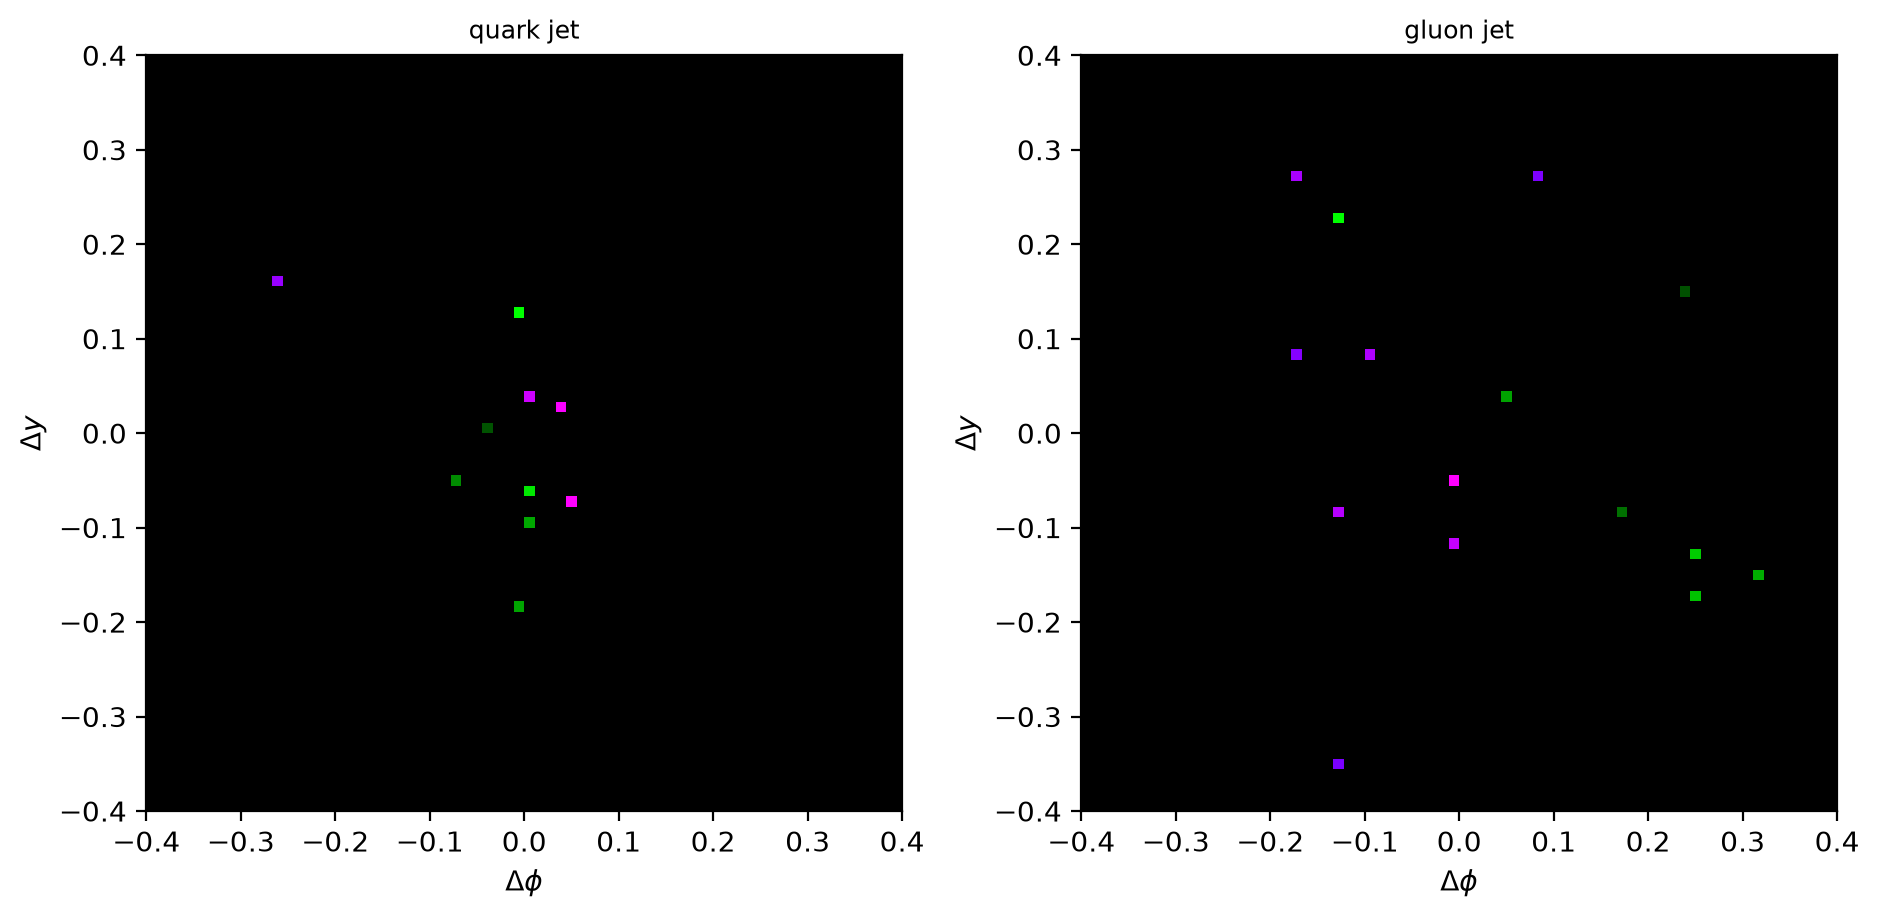
\includegraphics[width=\linewidth]{figures/qgjet_images}
	\caption{Typical quark (left) and gluon (right) jet. Gluon jets exhibit a broader spatial radiation pattern
		and higher particle multiplicity compared to quark jets}
	\label{fig:qgjetimages}
\end{figure}

The images were input for a Convolutional Neural Network (CNN) implemented using PyTorch as shown in fig.~\ref{fig:rgbnn}.  
%
Each convolutional layer consisted of 64 filters, with filter sizes of 5×5, 3×3, and 3×3, respectively (8×8, 4×4, and 4×4 for the 72×72 images). The max-pooling layers performed a 2×2 down-sampling with a stride length of 2. The dense layer consisted of 128 units, with a dropout rate of 0.2 before and after it.
\begin{figure}
	\centering
	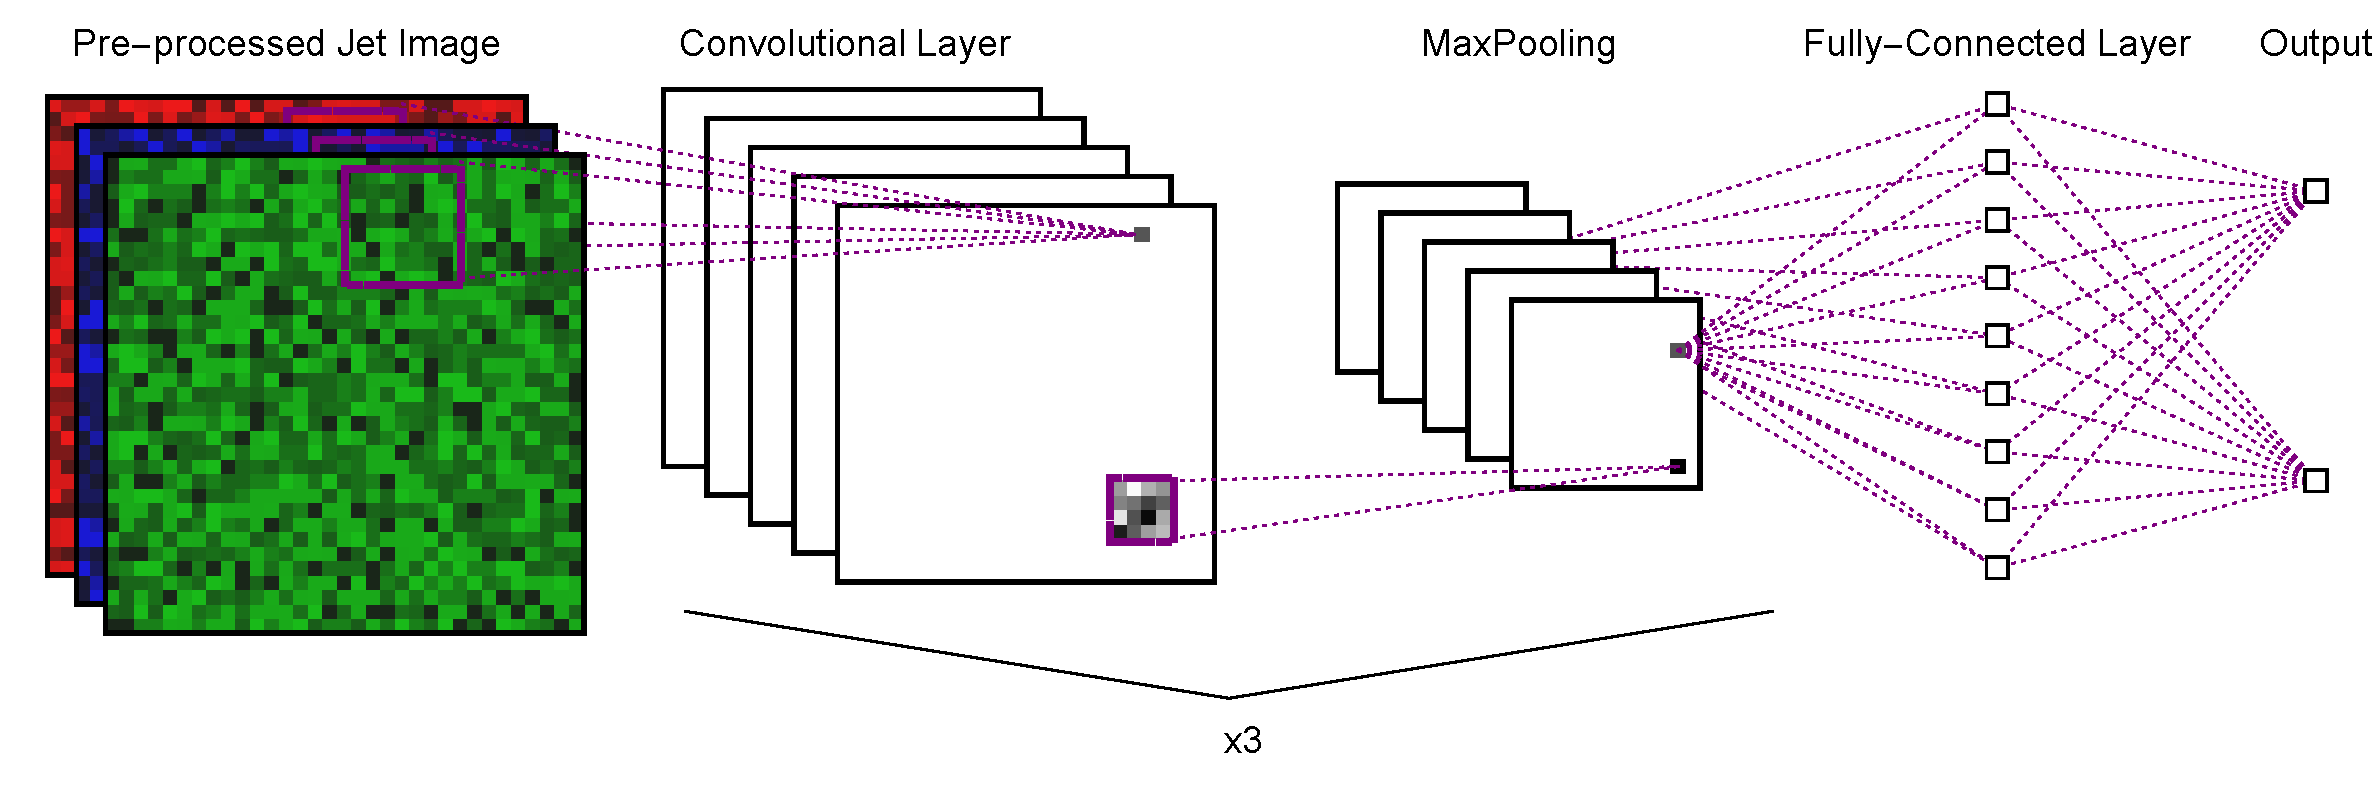
\includegraphics[width=1\linewidth]{figures/RGBNN}
	\caption{An illustration of the deep convolutional neural network architecture. The first
		layer is the input jet image, followed by three convolutional layers, a dense layer and an
		output layer.~\cite{Komiske_2017}}
	\label{fig:rgbnn}
\end{figure}

The network was trained with the AdamW optimizer at a learning rate of \(10^{-3}\) and a weight decay of 0.1, using the cross-entropy loss. 
%
Training used a batch size of 128 for 20 epochs, and the model with the lowest validation loss was retained. 
%
\begin{figure}
	\centering
	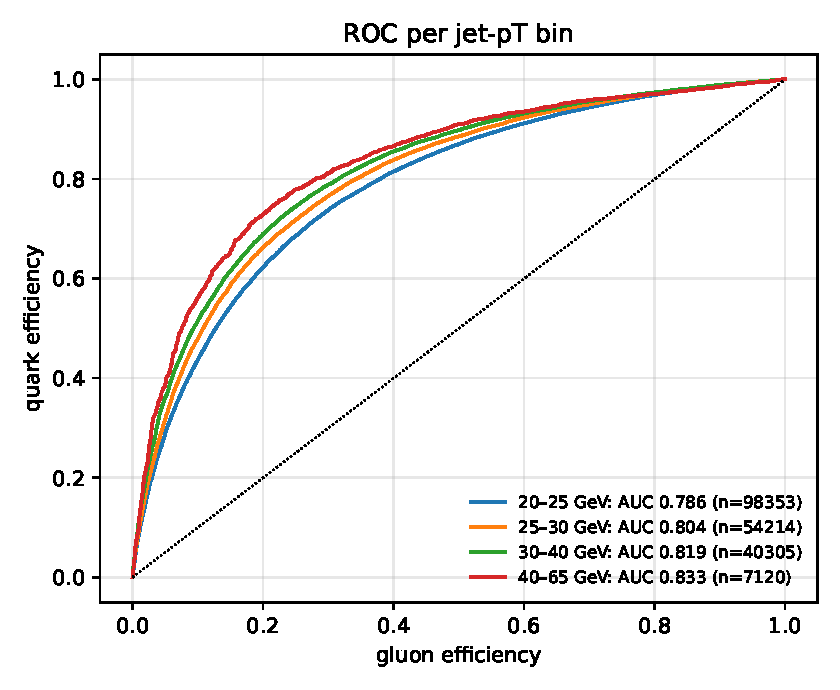
\includegraphics[width=0.7\linewidth]{figures/roc_per_jpt}
	\caption{}
	\label{fig:rocperjpt}
\end{figure}
Training images were augmented with random reflections in \(\Delta\eta\) and \(\Delta\phi\) and random translations of up to 0.5 pixels. 
%
The Receiver Operator Characteristic (ROC) curve  is shown differential in \(p_\mathrm{T, jet}\) by evaluating the model on a holdout test set.  


A way to gain some understanding of how the model looks at jet substructure is through \emph{interpretability} methods. 
%
We use a simple method of just noting the average change in classifier output upon masking a pixel. As seen in fig.~\ref{fig:importancecnnqg}, 
\begin{figure}
	\centering
	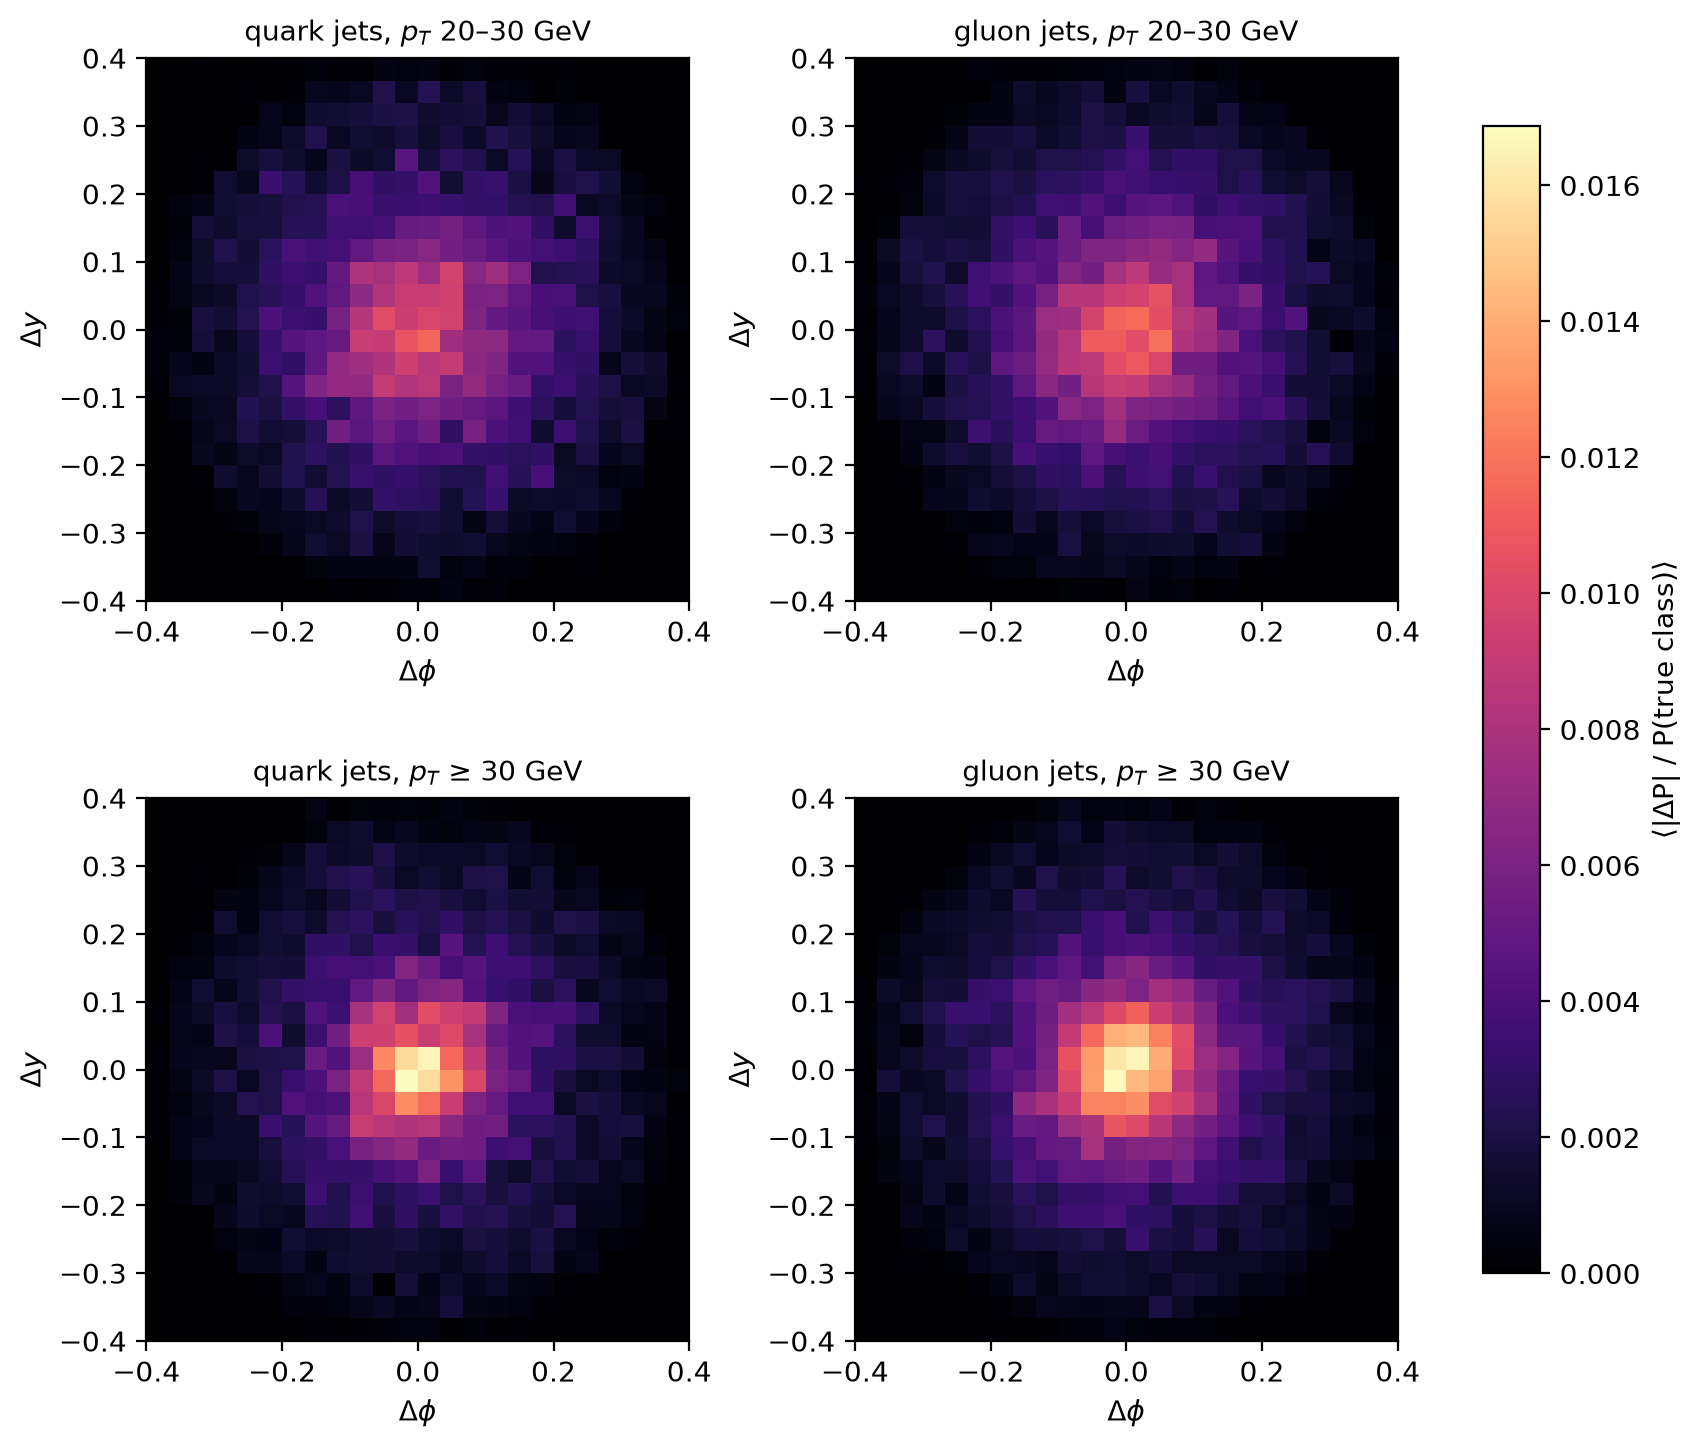
\includegraphics[width=0.7\linewidth]{figures/importance_cnn_qg}
	\caption{Per-pixel feature importance }
	\label{fig:importancecnnqg}
\end{figure}
\subsection{Characterizing jet quenching}
Another way to think about jet quenching/modification, is to ask how easily can a classifier algorithm tell apart the quenched and unquenched jet. 
%
Here we take PYTHIA-6~\cite{Sj_strand_2006} as the source of unquenched jets and JEWEL \cite{Zapp:2013vla} generates quenched jets in different centrality bins with/without recoil centers. 
%
Jets are represented as a 9-D vectors of features: $p_{\rm T, jet}$, $\rm N^{charged}_{\rm constit., jet}$, $\rm N^{neutral}_{\rm constit., jet}$, LeSub, $\lambda^2_0$, $\lambda_1^{0.5}$, $\lambda_1^1$, $\lambda_1^2$.
%
The jets are input into Dense Neural Networks (DNNs) with three hidden layers with 100 nodes each. After training, we calculate ROC curves shown in~\ref{fig:jetQuenchROC} using a holdout test set.
%
 \begin{figure}
 	\label{fig:jetQuenchROC}
	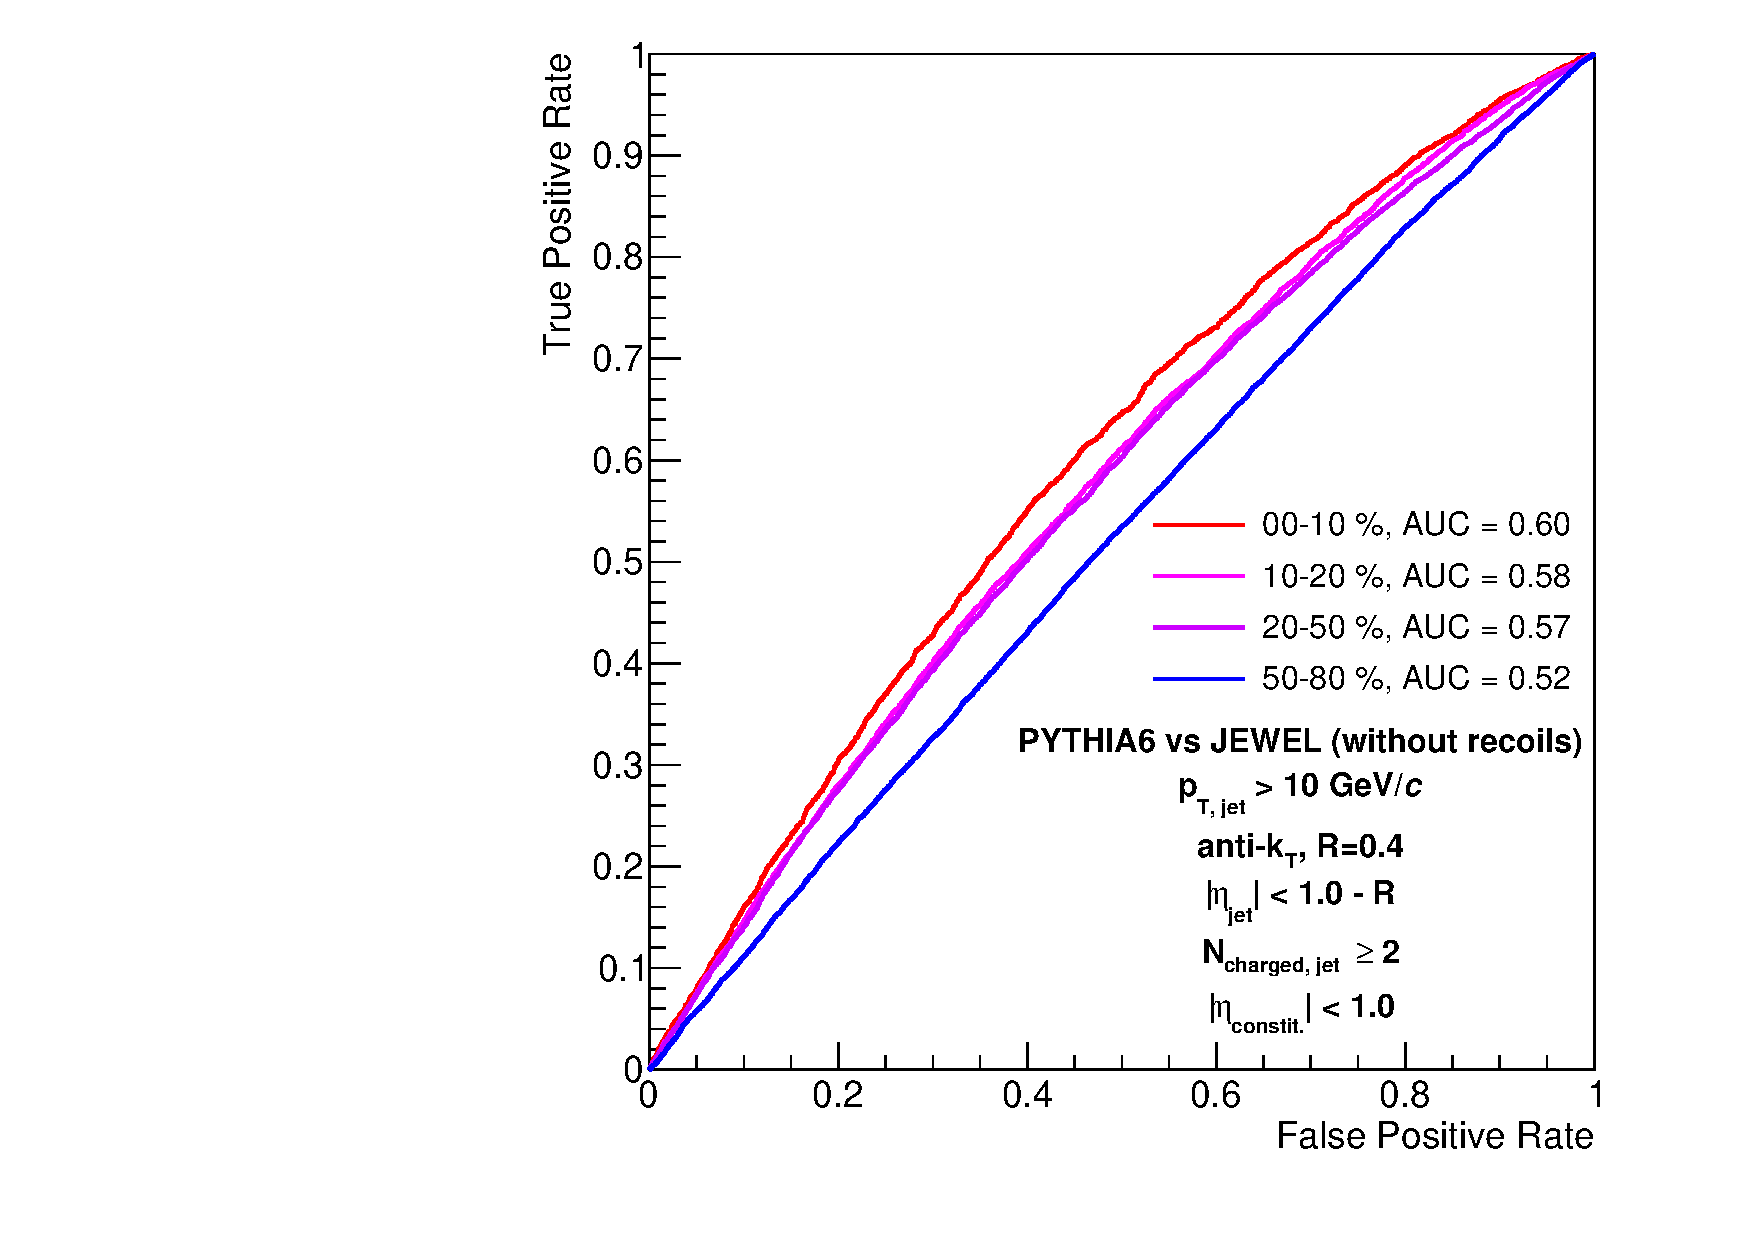
\includegraphics[width=0.49\linewidth]{roc_curve_dnn_withoutRec.pdf}
	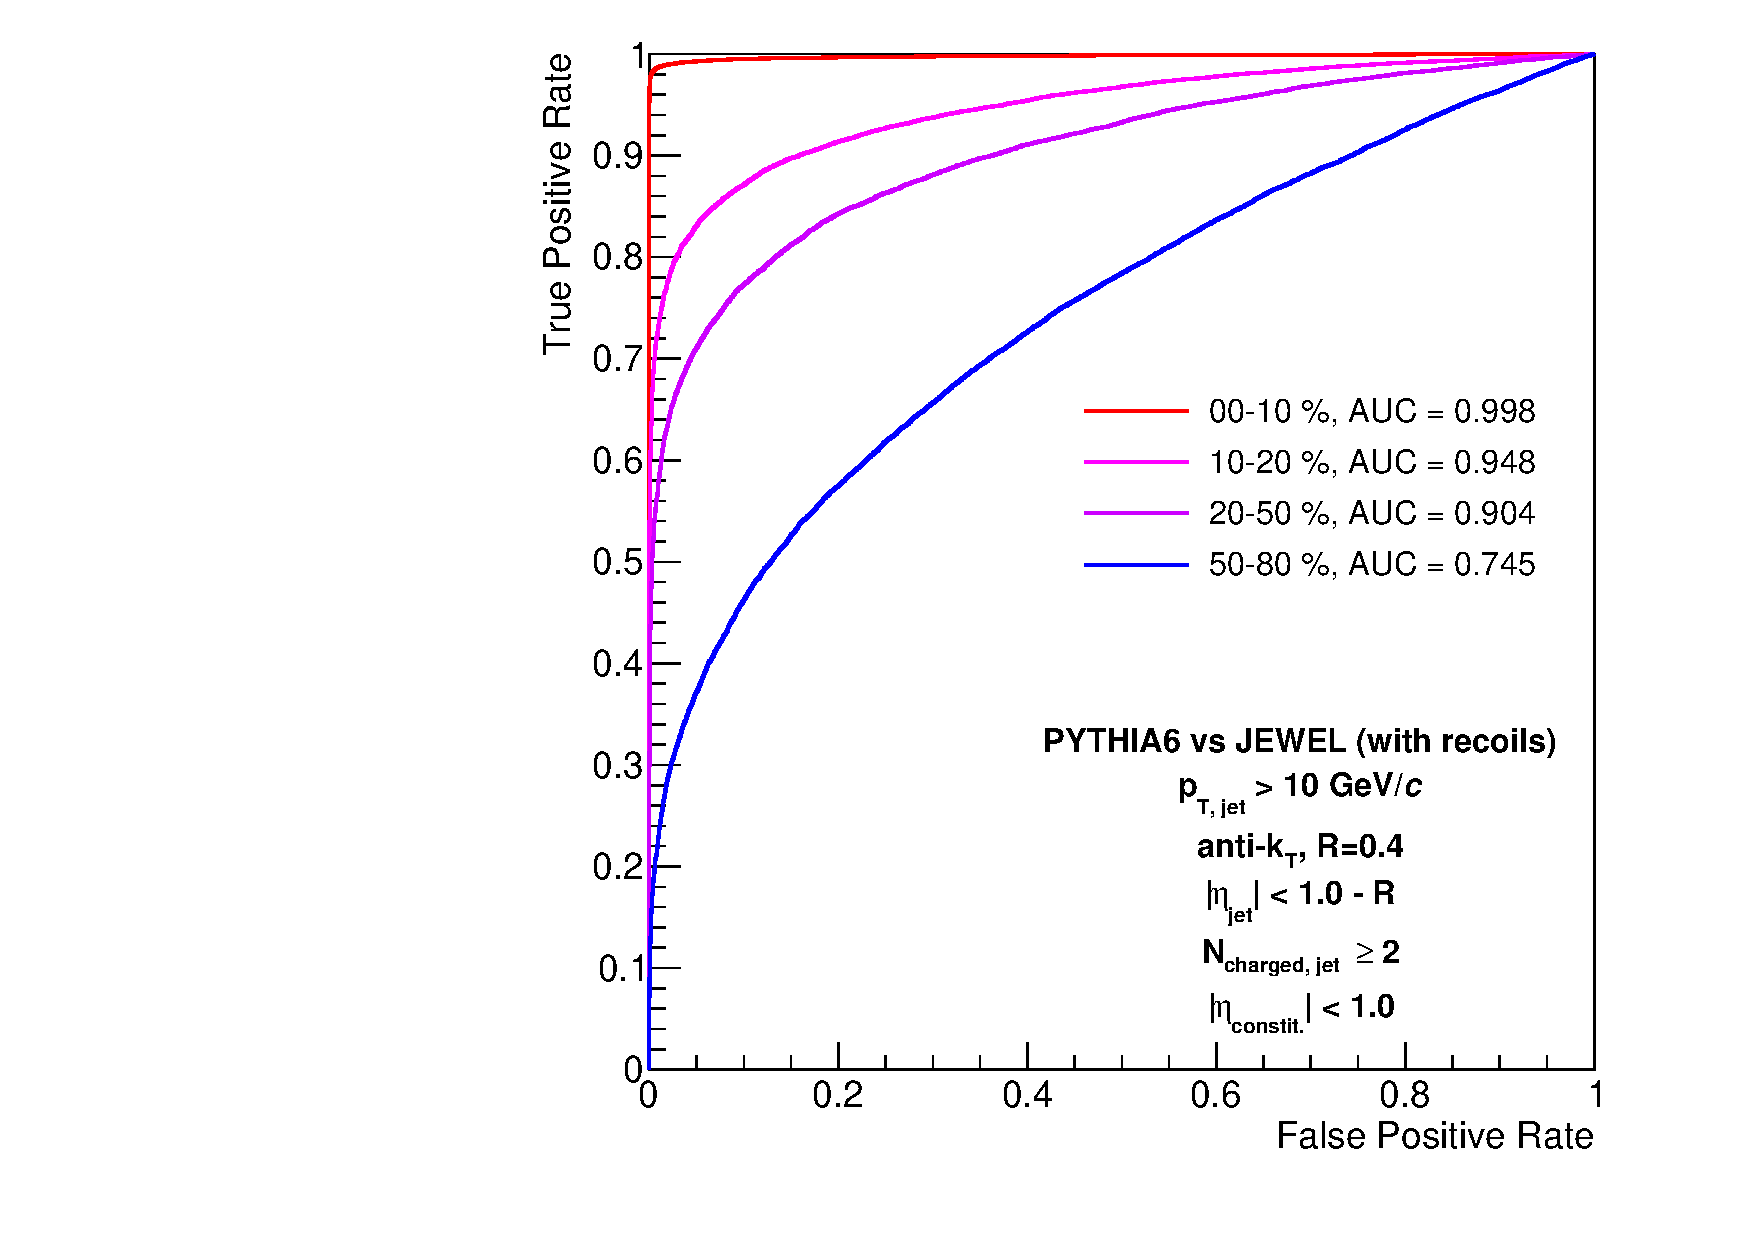
\includegraphics[width=0.49\linewidth]{roc_curve_dnn_wRec.pdf}
	\caption{ROC curves for PYTHIA6 vs. JEWEL without recoils (left) and with recoils (right).}
\end{figure}
%
The DNN performs better than chance in all the centralities and for both with/without recoils case.
The with-recoils case gives exagerrated ROC curves due to the background of recoil centers. 
%
AUC score decreases from central (0-10\%) to peripheral (50-80\%) events possibly implying more modification in central compared to peripheral.  
%
More information about jet quenching and machine learning can be found in~\cite{lai2022informationcontentjetquenching}

\section{Unfolding}
For any experiment, there is a disconnect between the desired phenomena (\emph{truth} level) and the measurement (\emph{measured} level) due to limitations of the detector setup. This is portrayed in fig.~\ref{fig:UnfoldingScheme} through a dijet event at the truth level, whose final state charged and neutral particles are recorded as TPC tracks and BEMC towers.  Each of the detectors smear the energy and momenta and for almost all experiments,  the information about particle species is lost. For example, at STAR often a \(\pi^0\) mass assumption is taken for measured constituents. Thus jets, which are composite objects of these tracks and towers are non-trivially modified by a complicated convolution of these effects. Even with the best background removal procedure, jets will contain some residual background fluctuations from the underlying event.

\begin{figure}[h]
	\centering
	\label{fig:UnfoldingScheme}
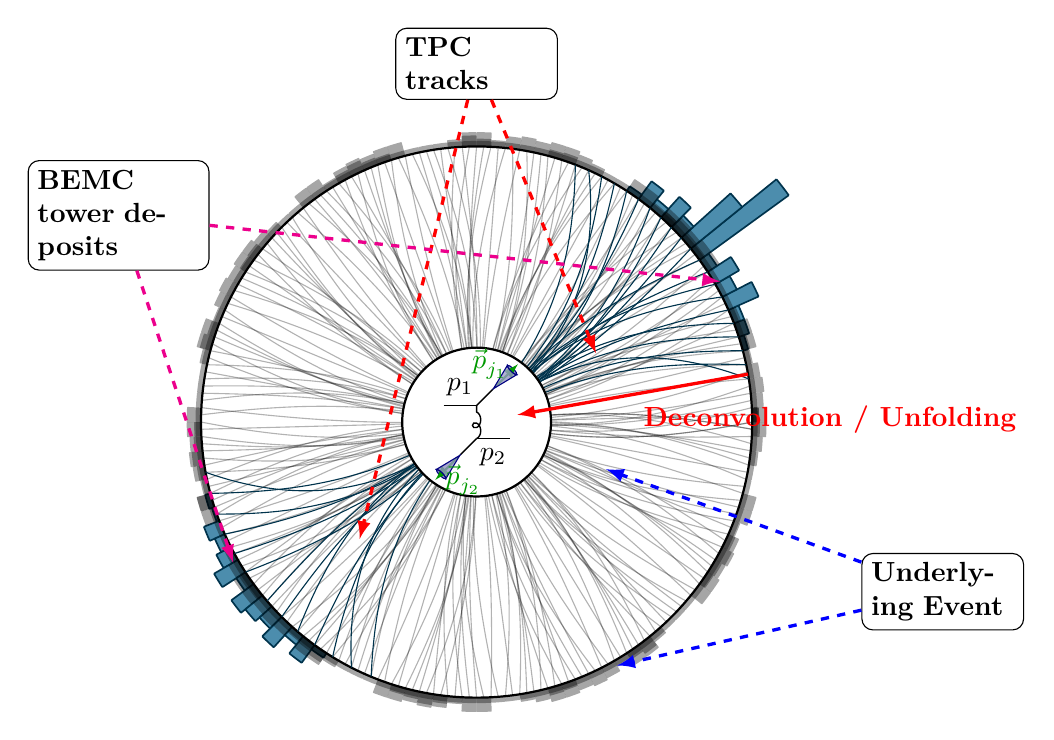
\begin{tikzpicture}[scale=0.7,rotate=0]
	\def\R{5} % tracker outer radius
	\def\dang{3} % angular granularity of calo deposits, 
	% HCAL DEPOSITS
	\foreach \dr [count=\i,
	evaluate={\r=\R+\dr; \anga=12+\dang*\i; \angb=\anga+\dang;}
	] in {0.1, 0.2, 0.2, 0.6, 0.3,0.5,0.2,2.0,1.2,0.3,0.5, 0.2, 0.4, 0.1}{
		\draw[calo] (0,0) -- (\anga:\r) arc(\anga:\angb:\r) -- cycle;
		%\draw[calo]
		%  (\anga:\R) -- (\anga:\r) arc(\anga:\angb:\r)
		%  -- (\angb:\R) arc(\angb:\anga:\R) -- cycle;
	}
	
	\foreach \dr [count=\i,
	evaluate={\r=\R+\dr; \anga=192+\dang*\i; \angb=\anga+\dang;}
	] in {0.1, 0.05, 0.3, 0.2,0.3,0.5,0.2, 0.5,0.4,0.3,0.5, 0.2, 0.4, 0.1}{
		\draw[calo] (0,0) -- (\anga:\r) arc(\anga:\angb:\r) -- cycle;
		%\draw[calo]
		%  (\anga:\R) -- (\anga:\r) arc(\anga:\angb:\r)
		%  -- (\angb:\R) arc(\angb:\anga:\R) -- cycle;
	}
	
	\foreach \ang [count=\i, 
	evaluate={\stepa = 15;
		\stepb=\stepa+50;
		\ra=\R+0.25*sin(\dang*\i*10); 
		\rb=\R+0.2*cos(\dang*\i*15);
		\rc=\R+0.3*sin(\dang*\i*20);
		\rd=\R+0.1;
	}]in {0, 3,...,360}{
		\draw[calobg] (0,0) -- (\ang:\ra) arc(\ang:\ang+\dang:\ra) -- cycle;
		\draw[calobg] (0,0) -- (\ang:\rd) arc(\ang:\ang+\dang:\rd) -- cycle;
		\draw[calobg] (0,0) -- (\stepa*\dang+\ang:\rb) arc(\stepa*\dang+\ang:\stepa*\dang+\ang+\dang:\rb) -- cycle;
		\draw[calobg] (0,0) -- (\stepb*\dang+\ang:\rc) arc(\stepb*\dang+\ang:\stepb*\dang+\ang+\dang:\rc) -- cycle;
	}
	
	\draw[thick,fill=white] (0,0) circle(\R); 
	
	\foreach \ang [count=\i,
	evaluate={\bend=12*sin(20+\i*\dang*15)}]in {0, 3,...,360}{
		\draw[black,opacity=0.3,thin,fill=none]
		(0,0) to[bend right=\bend] (\ang:\R);
	}
	
	\foreach \ang [count=\i,
	evaluate={\bend=12*cos(\i*\dang*15)}]in {0, 3,...,360}{
		\draw[black,opacity=0.3,thin,fill=none]
		(0,0) to[bend left=\bend] (\ang-\dang*0.5:\R);
	}
	
	%\draw[calo]
	%  (\anga:\R) -- (\anga:\r) arc(\anga:\angb:\r)
	%  -- (\angb:\R) arc(\angb:\anga:\R) -- cycle;
	
	\foreach \bend [count=\i,
	evaluate={\anga=6+\dang*\i;}
	] in {30, 14, 15,18, 20, 12, 19, 17, 11, 12}{
		\draw[blue!60!green!50!black,thin,fill=none]
		(0,0) to[bend left=\bend] (\anga:\R);	
	}	
	
	\foreach \bend [count=\i,
	evaluate={\anga=72-\dang*\i;}
	] in {20, 30, 19, 18, 20, 12, 19, 17, 12, 10, 8}{
		\draw[blue!60!green!50!black,thin,fill=none]
		(0,0) to[bend right=\bend] (\anga:\R);
	}
	
	\foreach \bend [count=\i,
	evaluate={\anga=186+1.5*\dang*\i;}
	] in {30, 14, 20, 12, 11, 12}{
		\draw[blue!60!green!50!black,thin,fill=none]
		(0,0) to[bend left=\bend] (\anga:\R);
	}
	
	\foreach \bend [count=\i,
	evaluate={\anga=252-1.5*\dang*\i;}
	] in {20, 30, 19, 12, 19, 10, 8}{
		\draw[blue!60!green!50!black,thin,fill=none]
		(0,0) to[bend right=\bend] (\anga:\R);
	}
	
		\node[draw, text width=0.15\textwidth, rounded corners=4pt] (tracks) at (90:1.3*\R){
			\textbf{TPC tracks}
		};		
		\draw (tracks) edge[dashed,  ->, very thick, red] (225:0.6*\R);
		\draw (tracks) edge[dashed,  ->, very thick, red] (30:0.5*\R);
		
		\node[draw, text width=0.17\textwidth, rounded corners=4pt] (towers) at (150:1.5*\R){
			\textbf{BEMC tower deposits} 
		};		
		\draw (towers) edge[dashed,  ->, very thick, magenta] (210:1.02*\R);
		\draw (towers) edge[dashed,  ->, very thick, magenta] (30:1.02*\R);
		
		\node[draw, text width=0.15\textwidth, rounded corners=4pt] (UE) at (340:1.8*\R){
			\textbf{Underlying Event}
		};		
		\draw (UE) edge[dashed, ->, very thick, blue] (300:1.02*\R);
		\draw (UE) edge[dashed,  ->, very thick, blue] (340:0.5*\R);
		
		\draw[thick,fill=white] (0,0) circle(0.27*\R); 
		\begin{feynhand}[scale=0.3]
			\vertex (a)  at (-1, -2); 
			\vertex(b)  at (-2, 1); 
			\vertex (c)  at (0, -1); 
			\vertex (d)  at (0, 1);
			\propag [plain] (c) to (a);
			\propag [plain] (b) to  [edge label = $p_1$] (d);
			\propag [gluon] (c) to (d);
			\vertex(e) at (2, -1) ; 
			\vertex (f) at (1, 2);
			\propag [plain] (e) to [edge label = $p_2$](c);
			\propag [plain] (d) to (f);
			\coordinate (J1) at (2.5,3.5);
			\coordinate (J2) at (-2.5, -3.5);
			\jetcone{f}{J1}{0.4}{0.10}
			\jetcone{a}{J2}{0.4}{0.10}
			\node[vector,left] at (J1) {$\vv{p}_{j_1}$};
			\node[vector,right] at (J2) {$\vv{p}_{j_2}$};
		\end{feynhand}		
	
	\draw  (10:\R) edge["\textbf{Deconvolution / Unfolding}", ->, very thick, red] (10:0.15*\R);
\end{tikzpicture}
\caption{Schematic figure showing the unfolding procedure. The desired physics / truth / particle level is represented by the \(2\to 2\) feynman diagram in the middle. The blue (gray) tracks and tower deposits are the dijet (underlying) event as recorded by the TPC and BEMC. } 
\end{figure}

Thus distributions of any jet observable \(\mathbf{O}\) will have these \emph{detector effects} which will need to be removed in order for the measurement to be comparable to theory calculations. In other terms, a truth value of \(\mathbf{x}\) can manifest as a range of measured values \((\mathbf{x}_0, \mathbf{x}_1)\) similarly, a measured value of \(\mathbf{y}\) can come from a range of truth values \((\mathbf{y}_0, \mathbf{y}_1)\).  Thus, using Bayes theorem, the probability either measured value being  \(\mathbf{y}\)  or truth value being  \(\mathbf{x}\) would be,

\begin{align}
	\label{eq:trMeas}
	p_\mathrm{meas.}(\mathbf{y}) &= \int d\mathbf{x}~p_\mathrm{meas.|tr.}(\mathbf{y} |  \mathbf{x}) p_\mathrm{tr.}(\mathbf{x}) \notag\\
	p_\mathrm{tr.}(\mathbf{x}) &= \int d\mathbf{y}~p_\mathrm{tr.|meas.}(\mathbf{x} |  \mathbf{y}) p_\mathrm{meas.}(\mathbf{y})
\end{align}

\begin{figure}
	\centering
	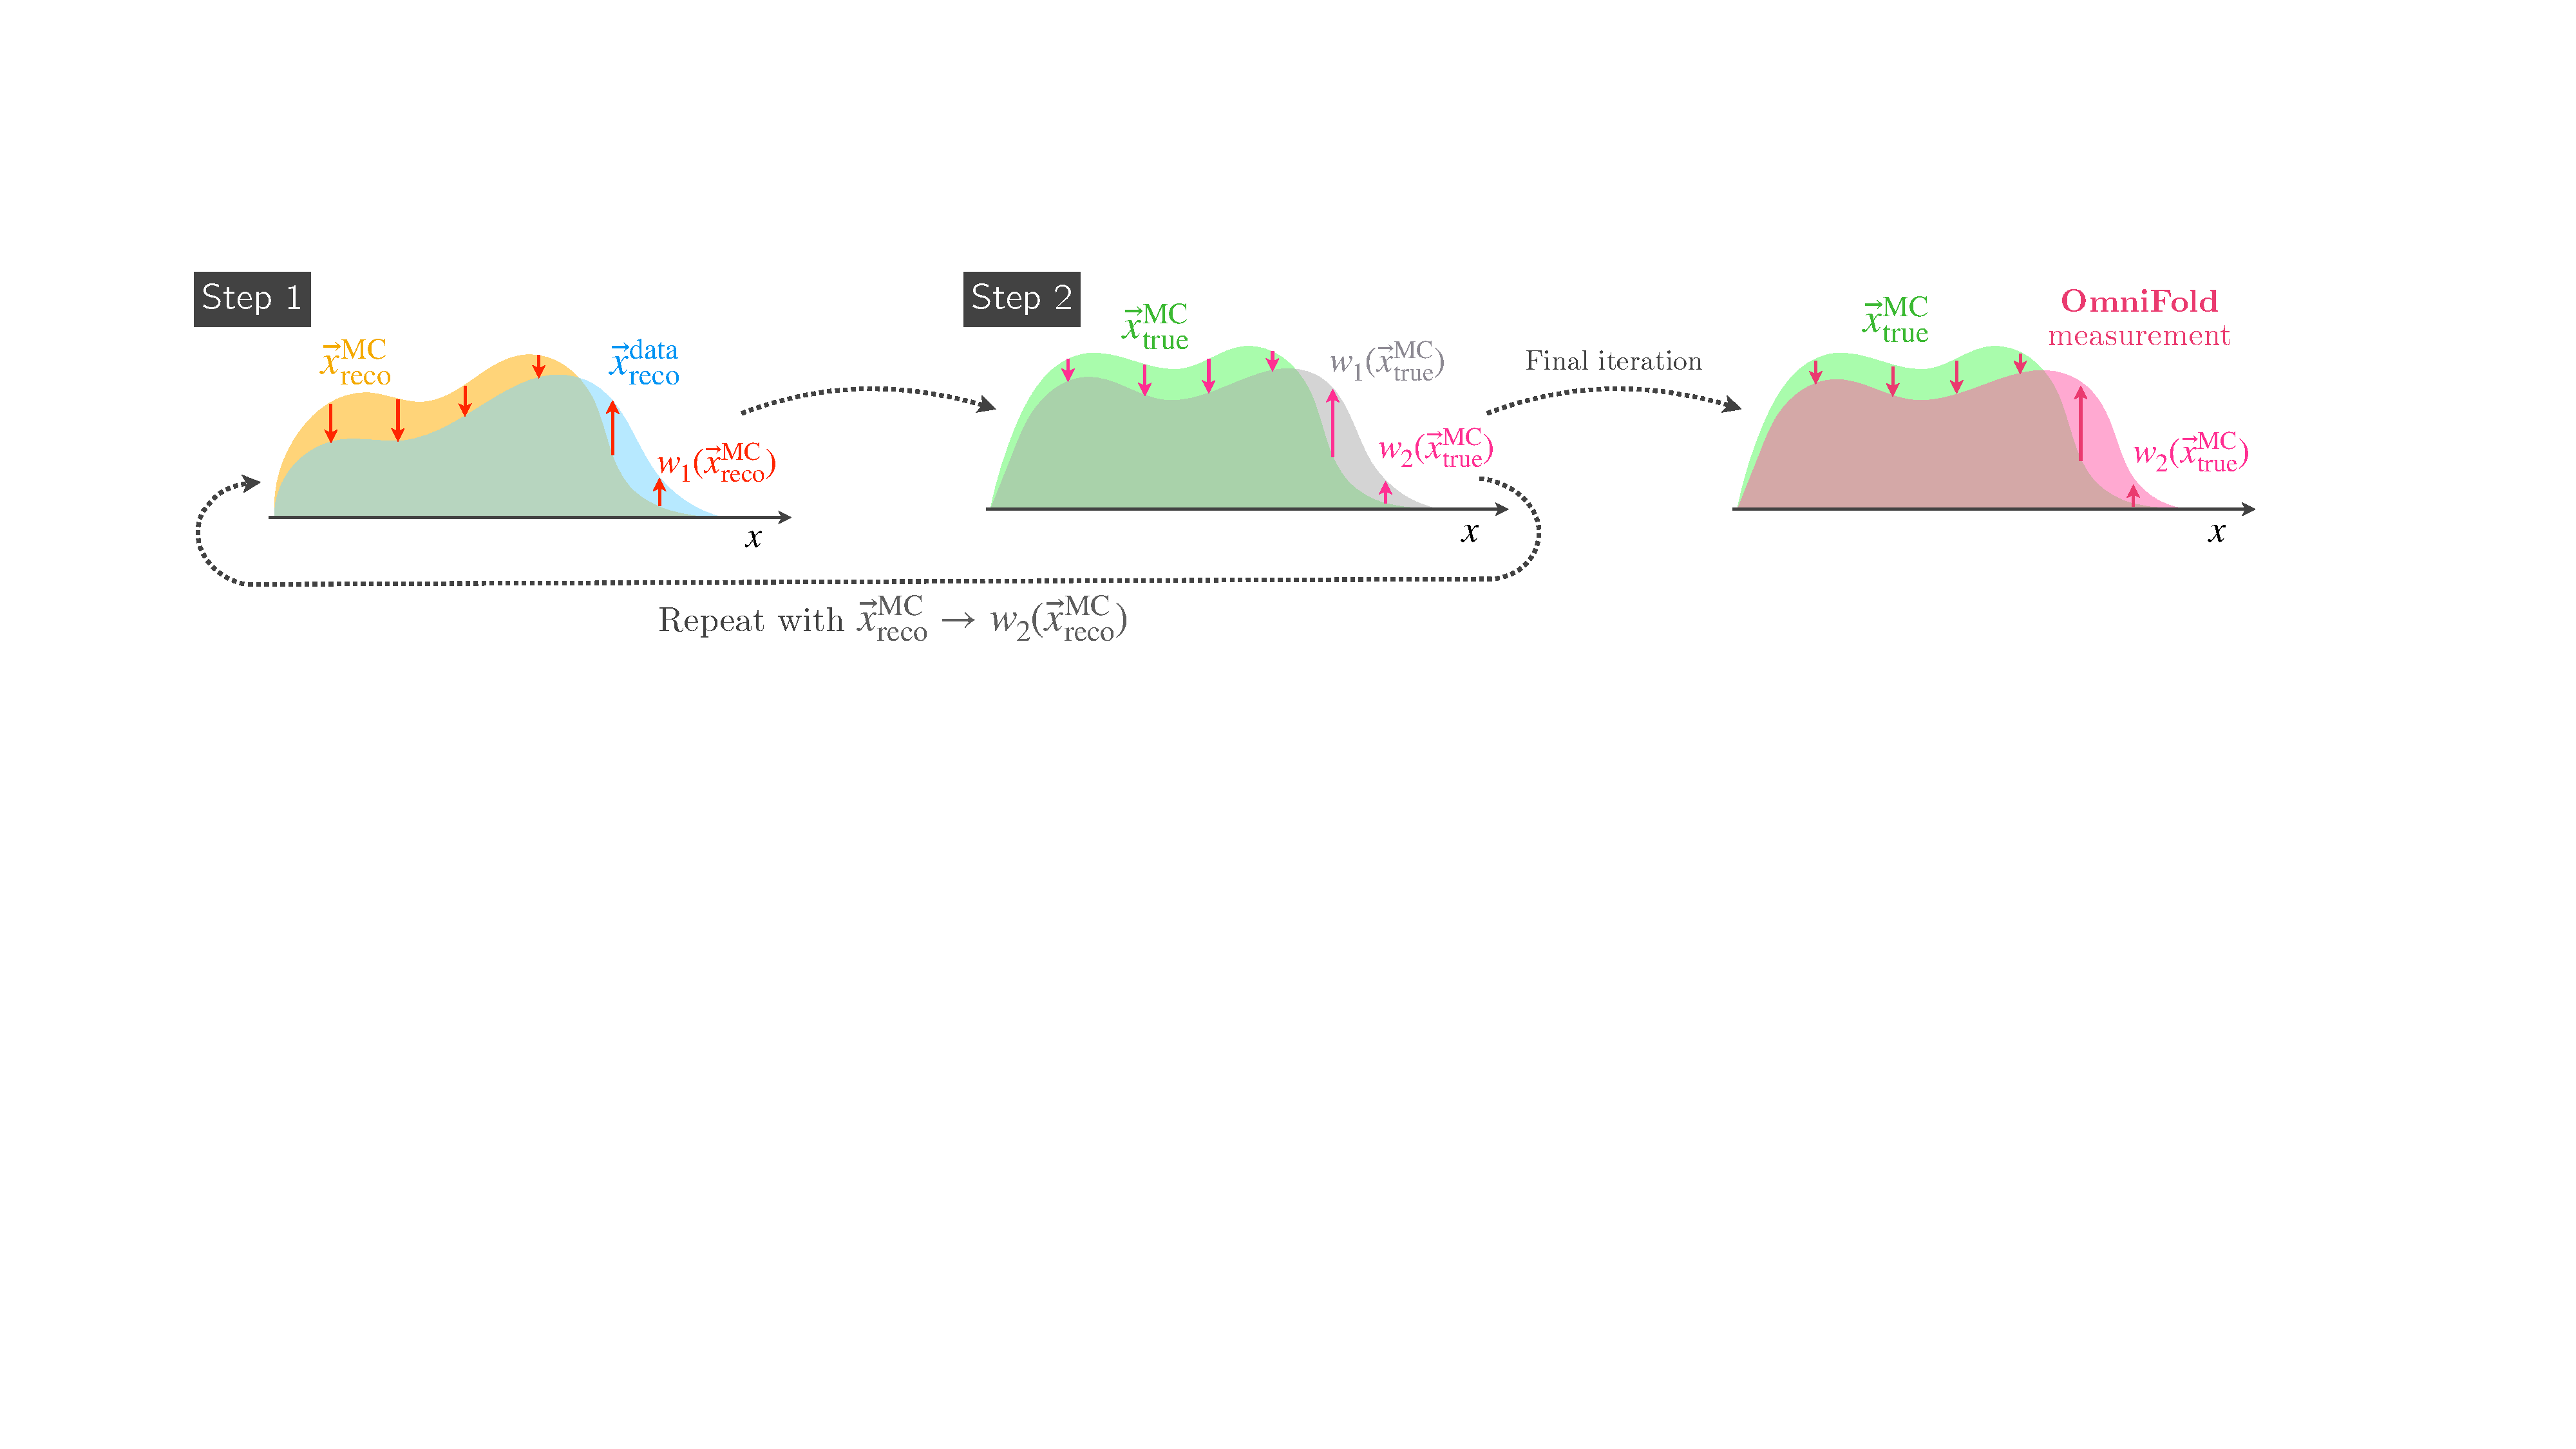
\includegraphics[width=1\linewidth]{figures/omnifold_fig_2025_04_24}
	\caption{Illustration of the OmniFold method. In Step 1, MC is corrected to match data at the detector level, producing a weighting function $w_1(\vec{x}_{\text{reco}}^{\text{ MC}})$. In Step 2, a new function $w_2(\vec{x}_{\text{true}}^{\text{ MC}})$ is learned based only on particle-level quantities. The method proceeds iteratively, refining the function $w_2(\vec{x}_{\text{true}}^{\text{ MC}})$ such that the particle-level MC can be reweighted to give event yields and kinematics that match those observed in the data.~\cite{Canelli_2026}
		\label{fig:omnifold}}
	\label{fig:omnifoldfig20250424}
\end{figure}

From eq.~\ref{eq:trMeas}, we measure \(p_\mathrm{meas.}\) through histograms, density estimates, etc. and \(p_\mathrm{tr.}\) is what we want to measure. Now, \(p_\mathrm{meas.|tr.}\) represents the detector's \emph{response}, which can be obtained to a high degree of accuracy from simulation programs like GEANT~\cite{MISC-15}. We can start from a \emph{generated} truth distribution  \(p_\mathrm{gen., 0}\) and obtain the \emph{reconstructed} measured distribution  \(p_\mathrm{reco., 0}\). Thus the assumption is, 
\begin{align}
	\label{eq:responseTransfer}
	p_\mathrm{meas.|tr.}(\mathbf{y} |  \mathbf{x}) = p_\mathrm{reco.|gen., 0}(\mathbf{y} |  \mathbf{x}) \equiv R(\mathbf{y}, \mathbf{x}) ,
\end{align}
Substituting \(R(\mathbf{y}, \mathbf{x})\) in eq.~\ref{eq:trMeas} and using \(\omega_0(\mathbf{y}) = p_\mathrm{meas.}(\mathbf{y})/p_\mathrm{reco., 0}(\mathbf{y})\)
\begin{align}
	\label{eq:unfoldEstimator}
	p_\mathrm{gen., 1}(\mathbf{x}) &\equiv \int d\mathbf{y}~p_\mathrm{gen.|reco., 0}(\mathbf{x} |  \mathbf{y})\,p_\mathrm{meas.}(\mathbf{y}) \notag\\
	&=\int d\mathbf{y}~\frac{R(\mathbf{y}, \mathbf{x})\,p_\mathrm{gen., 0}(\mathbf{x})}{p_\mathrm{reco., 0}(\mathbf{y})} p_\mathrm{meas.}(\mathbf{y})\notag\\
	&= p_\mathrm{gen., 0}(\mathbf{x})\int d\mathbf{y}~R(\mathbf{y}, \mathbf{x})\,\omega_0(\mathbf{y})
\end{align}
Using \(\nu_0(\mathbf{x}) = p_\mathrm{gen., 1}(\mathbf{x})/p_\mathrm{gen., 0}(\mathbf{x})\) measured distribution correspondingly becomes,
\begin{align}
	\label{eq:step2Joint}
	p_\mathrm{reco., 1}(\mathbf{y}) &= \int d\mathbf{x}~(\mathbf{x})\,R(\mathbf{y}, \mathbf{x})\,p_\mathrm{gen., 1}(\mathbf{x})\notag\\
	&= p_\mathrm{reco., 0}(\mathbf{y}) \int d\mathbf{x}~\frac{R(\mathbf{y}, \mathbf{x})\,p_\mathrm{gen., 0}(\mathbf{x})}{p_\mathrm{reco., 0}(\mathbf{y})}\nu_0(\mathbf{x}) 
\end{align}
The convolutions \(\int d\mathbf{y}~R(\mathbf{y}, \mathbf{x})\,\omega_0(\mathbf{y})\) and \(\int d\mathbf{x}~R(\mathbf{y}, \mathbf{x})\frac{\,p_\mathrm{gen., 0}(\mathbf{x})}{p_\mathrm{reco., 0}(\mathbf{y})}\nu_0(\mathbf{x})\) are mapping \(\omega_0(\mathbf{y})\to\omega_0(\mathbf{x})\) and \(\nu_0(\mathbf{x})\to\nu_0(\mathbf{y})\) respectively. 
%
For the \(n^\text{th}\) iteration, 
%
\begin{align}
	\label{eq:generalUnfolding}
	\omega_{n-1}(\mathbf{y}) &= \frac{p_\mathrm{meas.}(\mathbf{y})}{p_{\mathrm{reco.}, n-1}(\mathbf{y})} \notag\\
	p_{\mathrm{gen.}, n}(\mathbf{x}) &= p_{\mathrm{gen.}, n-1}(\mathbf{x})\int d\mathbf{y}~R(\mathbf{y}, \mathbf{x})\,\omega_{n-1}(\mathbf{y})\notag\\
	\nu_{n-1}(\mathbf{x}) &= \frac{p_{\mathrm{gen.}, n}(\mathbf{x})}{p_{\mathrm{gen.}, n-1}(\mathbf{x})} \notag\\
	p_{\mathrm{reco.}, n}(\mathbf{y}) &= p_{\mathrm{reco.}, n-1}(\mathbf{y}) \int d\mathbf{x}~R(\mathbf{y}, \mathbf{x})\frac{p_{\mathrm{gen.}, n-1}(\mathbf{x})}{p_{\mathrm{reco.}, n-1}(\mathbf{y})}\nu_{n-1}(\mathbf{x}) 
\end{align}
%
Given convergence, \(p_{\mathrm{reco.}, n}(\mathbf{y}) \to p_\mathrm{gen.}(\mathbf{y})\) and \(p_{\mathrm{tr.}, n}(\mathbf{x}) \to p_{\mathrm{unf.}}(\mathbf{x})\) is the unfolded distribution. 

%Generated jets without a reconstructed partner (\emph{misses}, \(\mathbf{y}=\varnothing\)) carry no \(\omega_{n-1}\), and reconstructed jets without a generated partner (\emph{fakes}, \(\mathbf{x}=\varnothing\)) carry no \(\nu_{n-1}\). Each receives its missing weight from the corresponding map of eq.~\ref{eq:generalUnfolding}, built from matched pairs and normalized over them,
%\begin{align}
%	\label{eq:missFakeWeights}
%	\omega_{n-1}(\mathbf{x}) &= \frac{\int d\mathbf{y}~R(\mathbf{y}, \mathbf{x})\,\omega_{n-1}(\mathbf{y})}{\int d\mathbf{y}~R(\mathbf{y}, \mathbf{x})}
%	= \frac{\int d\mathbf{y}~R(\mathbf{y}, \mathbf{x})\,\omega_{n-1}(\mathbf{y})}{\epsilon(\mathbf{x})} ,
%	&&\mathbf{y}=\varnothing , \notag\\
%	\nu_{n-1}(\mathbf{y}) &= \frac{\int d\mathbf{x}~R(\mathbf{y}, \mathbf{x})\,p_{\mathrm{gen.}, n-1}(\mathbf{x})\,\nu_{n-1}(\mathbf{x})}{\int d\mathbf{x}~R(\mathbf{y}, \mathbf{x})\,p_{\mathrm{gen.}, n-1}(\mathbf{x})} ,
%	&&\mathbf{x}=\varnothing ,
%\end{align}
%where \(\epsilon(\mathbf{x})\) is the reconstruction efficiency and the second denominator is \(p_{\mathrm{reco.}, n-1}(\mathbf{y})\) of matched jets. A miss at \(\mathbf{x}\) thus enters the second step with the mean first-step weight of the matched generated jets at \(\mathbf{x}\), and a fake at \(\mathbf{y}\) enters the next iteration with the weight the matched reconstructed jets at \(\mathbf{y}\) acquire from \(\nu_{n-1}\). Eq.~\ref{eq:generalUnfolding} then holds on the full samples,
%\begin{align}
%	\label{eq:missFakeIteration}
%	p_{\mathrm{gen.}, n}(\mathbf{x}) &= \omega_{n-1}(\mathbf{x})\,p_{\mathrm{gen.}, n-1}(\mathbf{x}) = \nu_{n-1}(\mathbf{x})\,p_{\mathrm{gen.}, n-1}(\mathbf{x}) , &&\text{matched and missed,} \notag\\
%	p_{\mathrm{reco.}, n}(\mathbf{y}) &= \nu_{n-1}(\mathbf{y})\,p_{\mathrm{reco.}, n-1}(\mathbf{y}) , &&\text{matched and fake,}
%\end{align}
%so that \(\nu_{n-1}\) is formed over a generated distribution that includes misses, and \(\omega_n\) against a reconstructed distribution that includes fakes.

This algorithm can be adapted for binned data by expressing the distributions as vectors representing bin counts of histograms and \(R(\mathbf{y}, \mathbf{x})\) as a matrix, giving the traditional method of \emph{Iterative Bayesian Unfolding}~\cite{bennerRoounfold}. Although it has been the standard for a long time, the required binning of data limits its usefulness beyond 3-dimensions. Also, not all measurements can be straightforwardly represented in the response matrix. 

One of the first unbinned approach uses classifiers to calculate ratios \(\omega\) and \(\nu\). For \(i^\text{th}\) iteration, \(\omega_{i-1}(\mathbf{y})\) can be calculated using classifier \(f_\mathrm{meas., reco}\) which classifies a jet represented by \(\mathbf{y}\) as measured or reconstructed. Thus, 
\begin{equation}
	\omega_{i-1}(\mathbf{y}) = \frac{f_\mathrm{meas., reco}(\mathbf{y})}{1 - f_\mathrm{meas., reco}(\mathbf{y})}
\end{equation}
and \(\nu_{i-1}(\mathbf{y})\) can be calculated using classifier \(f_{i, i-1}\) which classifies a jet represented by \(\mathbf{x}\) as being generated from \(i^\text{th}\) or \((i-1)^\text{th}\) iteration. 
\begin{equation}
	\nu_{i-1}(\mathbf{x}) = \frac{f_{i, i-1}(\mathbf{x})}{1-f_{i, i-1}(\mathbf{x})}
\end{equation}
 For misses, a classifier \(f^\mathrm{gen.}_{i, i-1}\) separates matched generated jets weighted by \(\omega_{i-1}(\mathbf{y})\) from those of the \((i-1)^\text{th}\) iteration; for fakes, a classifier \(f^\mathrm{reco.}_{i, i-1}\) separates matched reconstructed jets weighted by \(\nu_{i-1}(\mathbf{x})\) from those of the \((i-1)^\text{th}\) iteration,
\begin{equation}
	\omega_{i-1}(\mathbf{x}) = \frac{f^\mathrm{gen.}_{i, i-1}(\mathbf{x})}{1-f^\mathrm{gen.}_{i, i-1}(\mathbf{x})} ,
	\qquad
	\nu_{i-1}(\mathbf{y}) = \frac{f^\mathrm{reco.}_{i, i-1}(\mathbf{y})}{1-f^\mathrm{reco.}_{i, i-1}(\mathbf{y})} ,
\end{equation}
evaluated at the miss's \(\mathbf{x}\) and the fake's \(\mathbf{y}\) respectively. Thus, it takes 2-4 classfier training per unfolding iteration~\cite{andreassen2021scaffoldingsimulationsdeeplearning}.

\section{Bootstrap Uncertainties}
\label{sec:bootstrap}
The classifiers of the previous section are trained on finite samples of measured, reconstructed and generated jets, and the training itself is stochastic through the initialization of the model, dropout and the order of the mini-batches. 
%
The unfolded distribution inherits all of these, and after several trainings chained across iterations there is no closed form for propagating them. 
%
Instead, the whole procedure is repeated on resampled inputs and the spread of the outcomes is taken as the uncertainty. 

Every classifier \(f\) is replaced by an ensemble of \(N_\mathrm{rep.}\) replicas. 
%
Replica \(r\) is trained on a random subsample of \(m\) jets drawn without replacement from each of the two classes it separates (e.g. \(m\) measured and \(m\) reconstructed jets for \(f_\mathrm{meas., reco}\)), split further into a training and a validation set, with its own initialization and dropout. 
%
The same replica index is carried through every classifier of every iteration, so replica \(r\) is a complete unfolding on its own, with weights \(\omega^{(r)}_{n-1}\) and \(\nu^{(r)}_{n-1}\) and, from eq.~\ref{eq:generalUnfolding},
\begin{equation}
	\label{eq:replicaWeight}
	p^{(r)}_{\mathrm{gen.}, n}(\mathbf{x}) = p_{\mathrm{gen.}, 0}(\mathbf{x})\prod_{k=0}^{n-1}\nu^{(r)}_k(\mathbf{x}) \equiv w^{(r)}_n(\mathbf{x})\,p_{\mathrm{gen.}, 0}(\mathbf{x})
\end{equation}
Where, \(w^{(r)}_n(\mathbf{x})\) is the per-jet unfolding weight of replica \(r\) after \(n\) iterations. 
%
The subsampling is only done for training; at inference every replica is evaluated on every jet, so eq.~\ref{eq:replicaWeight} gives \(N_\mathrm{rep.}\) unfolded samples, each with the full statistics of the simulation. 

Any binned quantity \(H\), a histogram, a profile or a ratio of two of them, is then calculated once per replica from the weights \(w^{(r)}_n\), and its central value and uncertainty are the mean and standard deviation over the ensemble,
\begin{equation}
	\label{eq:bootstrapUnc}
	\bar{H} = \frac{1}{N_\mathrm{rep.}}\sum_{r=1}^{N_\mathrm{rep.}} H^{(r)} , \qquad
	\sigma_H^2 = \frac{1}{N_\mathrm{rep.} - 1}\sum_{r=1}^{N_\mathrm{rep.}}\left(H^{(r)} - \bar{H}\right)^2 
\end{equation}
Ratios are formed replica by replica before averaging, so the correlation between numerator and denominator through the shared weights is kept. 
%
Where a single diverged replica would pull \(\bar{H}\), the median or a trimmed mean over the ensemble is used for the central value instead; \(\sigma_H\) is always the standard deviation. 

Since the replicas differ in the measured subsample, the simulated subsample and the training, \(\sigma_H\) contains the statistical uncertainty of the measurement, that of the simulation and the variance of the training procedure, without separating them. 
%
With \(m\) smaller than the full samples, the spread is that of samples of size \(m\) and is conservative for the purely statistical part. 
%
\(N_\mathrm{rep.}\) only sets how precisely \(\sigma_H\) itself is known, not its size. 

\section{Barlow Test}
\label{sec:barlow}
The ensembles of Sec.~\ref{sec:bootstrap} are also used to decide whether a systematic variation is significant. 
%
Each variation is a complete unfolding with its own ensemble, giving \(\bar{H}_\mathrm{var.}\) and \(\sigma_\mathrm{var.}\) alongside the nominal \(\bar{H}_\mathrm{nom.}\) and \(\sigma_\mathrm{nom.}\). 
%
The shift \(\bar{H}_\mathrm{var.} - \bar{H}_\mathrm{nom.}\) is partly a statistical fluctuation between two ensembles, whose size is estimated as \(\sigma^2_\mathrm{uncorr.} = |\sigma^2_\mathrm{var.} - \sigma^2_\mathrm{nom.}|\), and the shift is only counted as a systematic uncertainty in a bin where
\begin{equation}
	\label{eq:barlow}
	\frac{|\bar{H}_\mathrm{var.} - \bar{H}_\mathrm{nom.}|}{\sigma_\mathrm{uncorr.}} \geq 1 ,
\end{equation}
the \emph{Barlow test}, and is set to zero otherwise. 






\chapter{Jet-Hadron Correlations Relative to the Event Plane}
\label{ch:jhcorr}
\begin{itquote}
This chapter is based on \cite{STAR:2023hye} published in \href{https://doi.org/10.1103/PhysRevC.109.044909}{Physical Review C \textcopyright{} American Physical Society}; titled ``Jet-hadron correlations with respect to the event plane in \(\sqrt{s_\mathrm{NN}} = 200\)~GeV Au+Au collisions in STAR''; authored by the STAR Collaboration, with Joel A. Mazer, Tanmay Pani and Sevil Salur as principal authors.
\end{itquote}
As discussed in Sec.~\ref{sec:jetsInQGP}, a parton traversing the QGP loses energy, and the amount lost is expected to depend on the length of its path through the medium.
%
In a non-central collision the overlap region is elongated, so the path length of a jet depends on its direction relative to the event plane (Sec.~\ref{sec:flowIntro} and App.~\ref{sec:EP_Recon}), and this chapter describes the measurement of the distribution of charged hadrons around jets separately for jets at different angles to the event plane.
%
In this analysis, the coordinate system used to depict the distribution of associated particles is defined relative to a reconstructed jet, also called a \emph{trigger jet}. 
%
The distribution is thus given by:
%
\begin{equation}
	\frac{1}{N_{\rm trig}} \frac{d^2 N_{\rm assoc,jet}}{d\dphi d\deta},
	\label{Eq:JHCorrIntro}
\end{equation}
%
\noindent where $N_{\rm trig}$ is the number of trigger jets, $N_{\rm assoc,jet}$ is the number of associated particles, \dphi ($=|\phi_{\rm jet}-\phi_{\rm assoc}|$) is the azimuthal angle of the associated particles relative to the trigger jets, and \deta ($=|\eta_{\rm jet}-\eta_{\rm assoc}|$) is the difference in the pseudorapidities of the trigger jet and associated particle.  
%
When studying the \dphi distributions, a peak is observed at $\dphi = 0$ which is the triggered jet, referred to as the \emph{near-side}.  
%
Another peak which is seen near $\dphi = \pi$ is referred to as the \emph{away-side}.  
%
The away-side consists of the hadrons from the recoiling parton, i.e.\ the second jet of the back-to-back hard scattering.

The goal of this analysis is to study the conditional yield of associated particles, the width of the near- and away-side peaks (quantified using the Gaussian width) as a function of the angle between the jet axis and the event plane.  The yield is estimated by:
%
\begin{equation}
	\mathrm{Yield} = \frac{1}{N_{\rm trig}} \int_{c}^{d} \int_{a}^{b} 
	\frac{d^2N_{\rm assoc,jet}}{d\dphi d\deta}  d\dphi d\deta.
	\label{Eqtn:Yield}
\end{equation}
%
The integration limits are chosen based on practical considerations, including the detector acceptance and binning of histograms.  

\section{Analysis method} \label{sect:Method}
This measurement utilizes data collected during the 2014 run from \AuAu collisions at nucleon-nucleon center-of-mass energy of \sNN{200}{GeV} by the STAR experiment~\cite{ACKERMANN2003624} at RHIC.  Events referred to as signal (same) events are required to fire the high-tower (HT2) trigger of the BEMC~\cite{BEDDO2003725}, which requires a single BEMC tower with a transverse energy above approximately 5.4~GeV.  Minimum-bias (MB) triggered events based on coincidence of Zero Degree Calorimeters (ZDC coincidence), Vertex Position Detectors (VPD) and Beam-Beam Counters (BBC) signals (Sec.~\ref{sec:triggerDetectors}) are used to estimate the pair-acceptance effects via a mixed-event (ME) technique \cite{PhysRevC.96.024905}. For this analysis, 9.4M HT-triggered and 4.0M MB collision events in the 20--50\% centrality range are used.

\subsection{Data set and event selection} \label{sec:JHEventSel}
The data consist of the mid- and low-luminosity subsets of the 2014 \AuAu production (830 and 548 runs, respectively).
%
Runs are rejected when run-averaged quantities of the MB events, namely the mean primary-vertex position along the beam $\langle v_z \rangle$ and in the transverse plane $\langle V_r \rangle$, the ZDC coincidence rate $\langle \mathrm{ZDCx} \rangle$, the reference multiplicity $\langle \mathrm{refMult} \rangle$, and the mean track transverse momentum, lie more than three standard deviations from their average over all runs; such outliers indicate detector or beam conditions that are not representative of the data set.

Events are required to have a reconstructed primary vertex within $|v_{z}| < 24$~cm of the center of the detector.
%
The pseudorapidity acceptance of the TPC changes with the vertex position, and the MB sample used for the event mixing (Sec.~\ref{sect:MixedEvents}) contains very few events at large $|v_z|$, which would limit the precision of the acceptance correction; the value of 24~cm was chosen by balancing the available statistics against the size of the resulting systematic uncertainties.
%
Events containing a track with $\ensuremath{p_{\rm T}}\xspace > 30$~\GeVc are rejected, since such tracks are dominated by cosmic rays and mis-reconstructed tracks for which the TPC momentum resolution is poor.

The centrality of each event, defined in Sec.~\ref{sect:CentEP}, is determined from the charged-particle multiplicity measured in the TPC within $|\eta| < 0.5$ (refMult) using the standard STAR procedure: refMult is corrected event-by-event for its dependence on the vertex position and on the luminosity, and the multiplicity distribution of the most peripheral events is corrected for the trigger inefficiency of the VPD using a Monte Carlo Glauber simulation.
%
The 20--50\% centrality range used here corresponds approximately to corrected refMult values of 75--250.
%
To increase the number of events available for the event mixing by more than 60\%, events from two MB triggers with different online VPD vertex requirements are combined: VPDMB5 and VPDMB30, which require the vertex position reconstructed online from the VPD timing to lie within \(|v_{z}| < 5\)~cm and \(|v_{z}| < 30\)~cm of the center of the detector, respectively.
%
The VPDMB5 events are reweighted in bins of refMult and $v_z$ so that their multiplicity distributions match those of the VPDMB30 events, which compensates for the different VPD resolution and the offset of the online VPD vertex cut, and they are only used for $|v_z| < 16$~cm; events in which both triggers fired are used only once.

\subsection{Track and tower selection} \label{sec:TrackTowerSel}
Charged tracks are reconstructed in the TPC and are required to be primary tracks, i.e.\ to be consistent with originating from the primary vertex.
%
The selection criteria, listed in Tab.~\ref{Tab:JHTrackCuts}, are designed to reject background tracks and to ensure a good momentum measurement.
%
The distance of closest approach (DCA) of the track to the primary vertex is required to be below 3~cm, which suppresses secondary particles from weak decays and interactions with the detector material, as well as tracks from pile-up collisions.
%
A minimum of 15 fit points in the TPC ensures a reliable curvature, and hence momentum, measurement, while requiring that at least 52\% of the possible fit points be used removes \emph{split tracks}, a single particle reconstructed as two track segments that would otherwise be counted twice.
%
Tracks below 0.2~\GeVc curl up in the magnetic field before crossing enough pad rows to be reconstructed reliably, and tracks above 30~\GeVc have a poor momentum resolution.
%
The acceptance $|\eta| < 1.0$ matches that of the BEMC.
%
Only tracks with $\ensuremath{p_{\rm T}}\xspace > 2.0$~\GeVc are used in the jet reconstruction (Sec.~\ref{sec:JetRecoAuAu}), while all selected tracks with $\ensuremath{p_{\rm T}}\xspace > 1.0$~\GeVc serve as associated particles.

\begin{table}[!htbp]
	\caption[Track selection criteria]{Track selection criteria.}
	\label{Tab:JHTrackCuts}
	\centering
	\begin{tabular}{l | c}
		\hline
		Criterion & Value \Tstrut \Bstrut \\
		\hline
		Primary track & yes \\
		DCA to the primary vertex & $< 3$~cm \\
		Number of fit points, $N_\mathrm{hits,fit}$ & $\geq 15$ \\
		$N_\mathrm{hits,fit}/N_\mathrm{hits,poss}$ & $\geq 0.52$ \\
		Pseudorapidity & $|\eta| < 1.0$ \\
		Transverse momentum & $0.2 < \ensuremath{p_{\rm T}}\xspace < 30$~\GeVc \\
		\hline
	\end{tabular}
\end{table}

The single-track reconstruction efficiency, $\epsilon(\Pt{assoc}, \eta_{\rm assoc})$ in Eq.~\ref{Eqtn:CorrFunction}, is the probability that a charged particle within the acceptance is reconstructed and passes the track selection.
%
To determine it, the detector response to simulated pions, kaons and protons is computed with the GEANT simulation of the STAR detector and embedded into real \AuAu events, which are then processed with the full STAR reconstruction chain.
%
The efficiency is the fraction of these embedded particles that are matched to a reconstructed track.
%
Since the efficiency decreases with the detector occupancy, it is evaluated as a function of \ensuremath{p_{\rm T}}\xspace and $\eta$ in bins of centrality and of luminosity.
%
It is approximately constant above 5~\GeVc, so the value at 4.5~\GeVc is used for all tracks above 5~\GeVc.
%
The correction is applied track-by-track to the associated hadrons in both the same and the mixed events.
%
A relative uncertainty of 5\% is assigned to the efficiency; it accounts for the imperfect description of the TPC response in the embedding and is the dominant contribution to the global scale uncertainty of the results (Sec.~\ref{sect:SysUnc}).

The BEMC towers are required to have $0.2 < E_\mathrm{T} < 30$~GeV and $|\eta| < 1.0$, with the tower transverse energy calculated with respect to the primary vertex.
%
Towers that are hot (firing too often or with too large energies), cold, or dead during the run period are excluded using a list of 452 bad towers, determined from their firing rates and energy distributions.
%
In addition, events in which the HT2 trigger was fired by one of these bad towers are rejected, so that a bad tower can neither contribute to a jet nor trigger an event.

Charged particles that leave a track in the TPC also deposit energy in the BEMC: charged hadrons as minimum-ionizing particles or partial hadronic showers, and electrons with nearly all of their energy.
%
Without a correction this energy would be counted twice in the jet reconstruction.
%
Following Ref.~\cite{STAR:2021lvw}, the momenta of all tracks that extrapolate to a given tower are subtracted from its energy,
%
\begin{equation}
	E_\mathrm{tower}^\mathrm{corr} = E_\mathrm{tower} - f_\mathrm{had} \sum_{\mathrm{matched}} p\,c,
	\label{Eq:HadCorr}
\end{equation}
%
with $f_\mathrm{had} = 1$, and the tower is removed if its corrected energy falls below the threshold required for the jet constituents.
%
Although subtracting the full track momentum over-corrects the charged hadrons, which deposit on average only about a third of their energy in the BEMC~\cite{STAR:2019yqm}, it removes the large tower-by-tower fluctuations of the deposited energy and therefore improves the jet energy resolution.

\subsection{Event plane reconstruction} \label{sec:EPReco}
The event plane (\(\Psi_{2,EP}\)), the experimental estimate of the reaction plane described in App.~\ref{sec:EP_Recon}, is calculated event-by-event using the Modified Reaction Plane (MRP) method~\cite{CASTILHO2018369,Agakishiev:2014ada,Adams_2005} using charged tracks with $0.2 < p_{\rm  T, track} < 1.0$ \GeVc measured within the TPC.  
%
The impact of highly energetic jets on the calculation of the event-plane orientation is reduced by removing the particles within the pseudorapidity strip ($|\deta|<0.4$) across \dphi surrounding the leading jet.  
%
This procedure also removes a significant portion of the away-side jet, located opposite in azimuth. 
%
The event plane is obtained from the $p_\mathrm{T}$-weighted second-order flow vector $\mathbf{Q}_2$ of these tracks (Eqs.~\ref{eqn:EP} and~\ref{Eqn:Qvecs}); the $p_\mathrm{T}$ weights are used because the flow coefficients grow approximately linearly with \ensuremath{p_{\rm T}}\xspace at low \ensuremath{p_{\rm T}}\xspace.
%
Restricting the event-plane tracks to $\ensuremath{p_{\rm T}}\xspace < 1.0$~\GeVc also avoids auto-correlations with the associated hadrons, which are measured above 1.0~\GeVc.
%
The non-uniform acceptance and efficiency of the TPC make the distribution of the reconstructed $\Psi_{2,EP}$ non-flat; this is corrected by re-centering $\mathbf{Q}_2$ and by the shift method up to the 20th order (App.~\ref{sec:EP_Recon}), with both corrections determined separately for 10\% centrality intervals and 4-cm $v_z$ intervals.
%

The distributions of the associated tracks relative to the trigger jet are measured in three bins in the angle between the trigger jet and the event plane,
%
\begin{equation}
	\begin{aligned}
		&\text{in-plane:}     && |\Psi_{2,EP}-\phi_{\mathrm{jet}}|<\pi/6,\\
		&\text{mid-plane:}    && \pi/6<|\Psi_{2,EP}-\phi_{\mathrm{jet}}|<\pi/3,\\
		&\text{out-of-plane:} && |\Psi_{2,EP}-\phi_{\mathrm{jet}}|>\pi/3,
	\end{aligned}
	\label{Eq:EPbins}
\end{equation}
%
where the angle difference is folded into $[0, \pi/2]$.
%
The analysis is restricted to 20--50\% central \AuAu collisions to achieve the highest event-plane resolution and therefore the analysis will be most sensitive to any path-length dependencies. 
%The possible impact of the finite event-plane resolution on the signal is discussed in Sec.~\ref{Sec:RxnPlaneResolutionEffects}.
% As in Fig.~\ref{plot:rxnschematic}, we see the event-plane orientations defined relative to a trigger (jet).
% \begin{figure}[!htbp]
	%   \begin{center}
		%     \rotatebox{0}{\resizebox{5cm}{!}{\includegraphics{figures/RxnPlaneFig.pdf} }}
		%     \caption{Jet-hadron correlations are measured in three regions relative to the $n=2$ reconstructed event plane.  These regions are defined as: in-plane ($|\psi-\phi_{\mathrm {jet}}| < \pi/6$) shown in red, mid-plane ($\pi/6 < |\psi-\phi_{\mathrm {jet}}| < \pi/3$) shown in white, and out-of-plane ($|\psi-\phi_{\mathrm {jet}}| > \pi/3$) shown in blue.  
			%   }\label{plot:rxnschematic}
		%   \end{center}
	% \end{figure}
% set up next section for centrality and event plane

The second- (fourth-) order event-plane resolutions relative to the second-order event plane ($R_2\{\Psi_{2, EP}\}$ and $R_4\{\Psi_{2, EP}\}$ respectively) as a function of collision centrality are shown in Fig.~\ref{fig:EPres}.  The resolution peaks in the 20--30\% and 30--40\% centrality classes.  %The event-plane resolutions are dependent on the momenta range of excluded tracks.
% For the momentum of the associated tracks used in this work, $R_2$ ranges from 0.52-0.66 and $R_4$ from 0.24-0.39.  
% This analysis used tracks from 0.2-1.0 \GeVc for event plane reconstruction to avoid having to use multiple event plane definitions or momentum exclusion ranges and to remove potential auto-correlations.  
Because of the finite number of particles, the reconstructed event plane only approximates the true symmetry plane; the resolution $R_n\{\Psi_{2,EP}\}$ (Eq.~\ref{resolution}) quantifies how well it does so.
%
It is determined from the data with the two-sub-event method (Eqs.~\ref{resolution2sub} and~\ref{resolutionIndiv}), in narrow centrality intervals that are combined over 20--50\% weighted by the number of events.
%
For 20--50\% central events, the event-plane resolutions $R_2\{\Psi_{2, EP}\}$ and $R_4\{\Psi_{2, EP}\}$ are 0.56 and 0.28, respectively.  The statistical uncertainties of the resolution are below 1\%; varying the resolution by $\pm 1\%$ has a negligible effect on the final \dphi correlations.  Measured values for the event-plane resolution are in good agreement with prior STAR studies \cite{Agakishiev:2014ada}.  The resolution enters the analysis in two places.
%
First, in the combinatorial background: its flow modulation, as seen relative to the reconstructed event plane, is described by the background fit of Sec.~\ref{sect:CorrBkgd}, which contains the resolutions \(R_n\) explicitly (Eqs.~\ref{Eq:vRn} and~\ref{Eq:betaR}), so that the background subtraction is corrected for the finite resolution.
%
Second, in the jet signal: the jets are sorted into the orientation bins of Eq.~\ref{Eq:EPbins} with the reconstructed event plane, so part of them end up in a different bin than their true orientation would put them in.
%
This is not corrected for; its size is estimated below.
% 2x1, width = 7.5cm
\begin{figure}[!htbp]
	\begin{center}     
		%  \includegraphics[width=7.5cm]{figures/plots/EPresolution/R2combined.pdf}
		%  \includegraphics[width=7.5cm]{figures/plots/EPresolution/R4combined.pdf}
		%   \includegraphics[width=7.5cm]{figures/plots/EPresolution/R02_1EP_C20-50.pdf}
		%   \includegraphics[width=7.5cm]{figures/plots/EPresolution/R04_1EP_C20-50.pdf}
		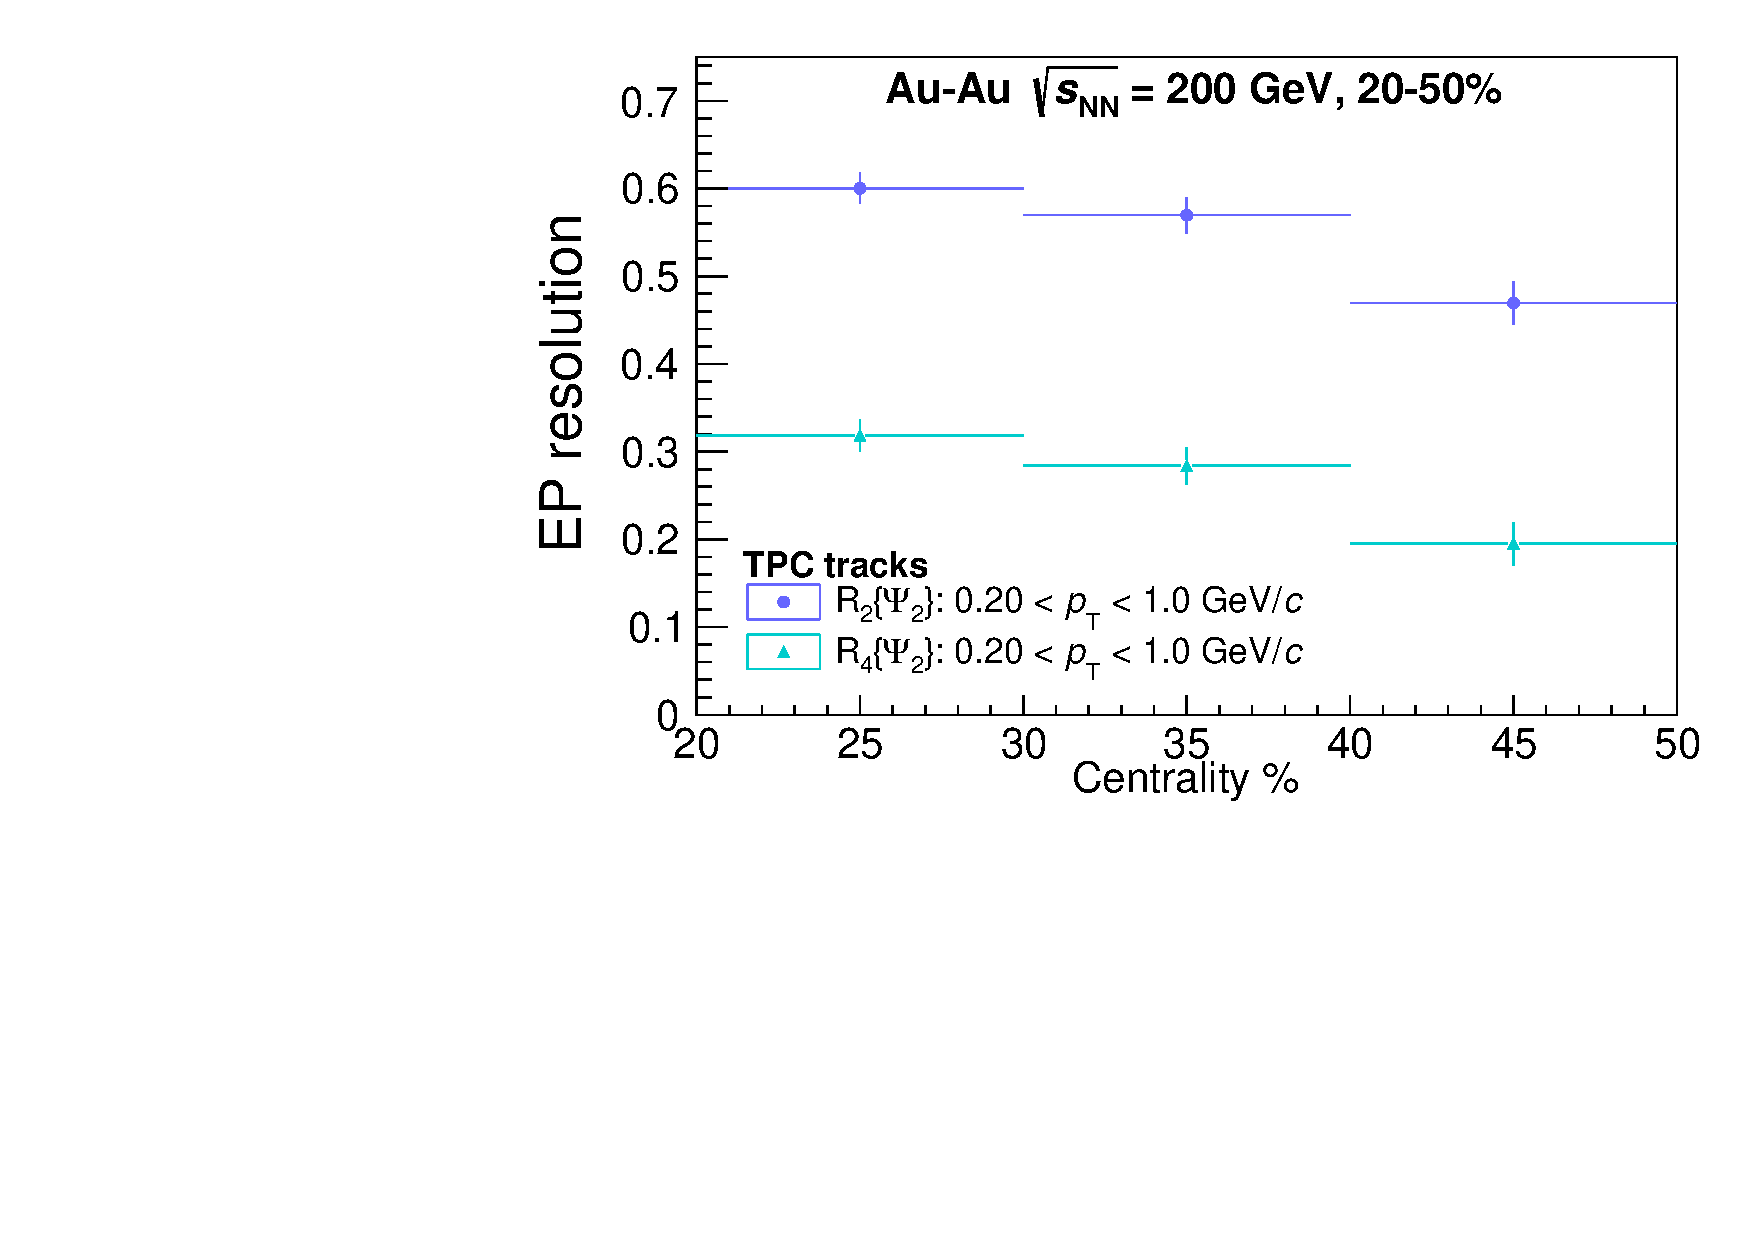
\includegraphics[width=12cm]{figures/R2-4combined.pdf}
		\caption[Event-plane resolution as a function of centrality]{Event-plane resolution: Second-order (fourth-order) harmonic relative to the event plane, $R_{2}(\Psi_{2})$ ($R_{4}(\Psi_{2})$), respectively.  The approach follows the Modified Reaction Plane (MRP) method \cite{Agakishiev:2014ada} utilizing the charged tracks of the TPC for event-plane reconstruction and resolution calculation for tracks with 0.2--1.0~\GeVc. Combined over 20--50\% centrality, $R_2 = 0.56$ and $R_4 = 0.28$. }  
		\label{fig:EPres}
	\end{center}
\end{figure}

Because the jets are sorted into the orientation bins with the reconstructed event plane, some in-plane jets are counted as mid- or out-of-plane and vice versa, which reduces any event-plane dependence of the signal.
%
This effect is not corrected for, since an unfolding of the orientation bins, or a Fourier decomposition of the signal, would require a precision the measurement does not have and would add further uncertainties.
%
Its size can instead be estimated with a simple model.
%
Suppose that path-length dependent jet quenching makes the associated yield per jet depend on the angle \(\Delta = \phi_\mathrm{jet} - \Psi_2\) between the jet and the \emph{true} symmetry plane as \(Y(\Delta) \propto 1 + 2 v_2^\mathrm{quench}\cos(2\Delta)\).
%
The coefficient $v_2^\mathrm{quench}$ is then the relative amplitude of this variation, in analogy with the flow coefficients of Sec.~\ref{sec:flowIntro}: for $v_2^\mathrm{quench} > 0$, in-plane jets, which traverse less medium, have larger associated yields than out-of-plane jets.
%
Measured relative to the reconstructed event plane, the variation is smeared, and its amplitude is reduced to $R_2 v_2^\mathrm{quench}$ (App.~\ref{sec:EP_Recon}).
%
Averaging $Y$ over the orientation bins of Eq.~\ref{Eq:EPbins} then gives, to first order in $v_2^\mathrm{quench}$, $Y_\mathrm{out}/Y_\mathrm{in} \approx 1 - (6\sqrt{3}/\pi) R_2 v_2^\mathrm{quench}$ and $Y_\mathrm{mid}/Y_\mathrm{in} \approx 1 - (3\sqrt{3}/\pi) R_2 v_2^\mathrm{quench}$.
%
The size of $v_2^\mathrm{quench}$ for the associated yields has not been measured.
%
As an illustration, $v_2^\mathrm{quench} = 0.1$ is taken, the upper end of the azimuthal anisotropy of the jet yields themselves measured at the LHC, between a few percent and about 0.1~\cite{ALICE:2015efi,ATLAS:2021ktw}, which arises from the same path-length dependence; whether the associated yields vary as strongly is not known.
%
With this value, the out-of-plane to in-plane (mid-plane to in-plane) yield ratio would be 0.67 (0.83) with a perfect event plane, but only 0.81 (0.91) with $R_2 = 0.56$, i.e.\ only about half of a real deviation from unity would remain visible.
%
The finite resolution therefore pulls any event-plane dependence of the yields toward unity, which must be kept in mind when interpreting the yield ratios in Sec.~\ref{sect:YieldRatio}.


\subsection{Jet reconstruction and selection} \label{sec:JetRecoAuAu}
Full jets are reconstructed by measuring charged tracks in the TPC and collecting neutral-particle information from the BEMC.  The anti-\kt algorithm 
%\cite{Cacciari:2008gp} implemented through the FastJet package \cite{Cacciari:2011ma} 
clusters these particles into jets by reconstructing the jet momenta as the quadratic sum of their constituent momenta using a boost-invariant $\it{p}^{2}_{\rm T}$ recombination scheme (Sec.~\ref{sec:jetAlgo}).  This scheme weights the directions of the constituents by $p^{2}_{\rm T}$ when they are combined, so that the jet axis follows the hardest constituents and is less sensitive to soft particles from the underlying event and from the recoil of the medium.  Tracks used for reconstructing jets are assumed to be pions while the towers to have arisen from massless particles. All jets measured in this work are clustered with resolution parameter of $R=0.4$. The area of jets, $A_{\rm jet}$, is found with FastJet using active ghost particles \cite{Cacciari:2008gn}.  Partially reconstructed jets at the edge of the acceptance are rejected by applying a fiducial cut, $|\eta_{\rm jet}| < 1.0 - R$, to assure all jets fall within the acceptance of the detectors. 

%This procedure uses the FastJet package \cite{Cacciari:2011ma}, where the anti-\kt \cite{Cacciari:2008gp} recombination algorithm is used for reconstructing signal jets and the \kt sequential recombination algorithm is used for estimating the underlying event background ($\rho$).  The momenta of the jet is calculated as the quadratic sum of their constituent momenta using a boost-invariant $\it{p}^{2}_{\rm T}$ recombination scheme.  Tracks used for reconstructing jets are assumed to be pions while the towers to have arisen from massless particles.  A jet can further be described by its resolution parameter $R$, which refers to its radial extension in azimuth and pseudorapidity.  The exact meaning of R is algorithm specific, but in this paper, it will typically refer to roughly circular clusters of radius R about the jet axis determined by $\Delta R = \sqrt{\dphi^2 + \deta^2}$ where \dphi (\deta) is the relative azimuthal angle (relative pseudorapidity).  The area of jets, $A^{jet}$, is found within the FastJet package utilizing active ghost particles \cite{Cacciari:2008gn}.  The location of a jet is described by the `jet axis', which refers to the azimuthal and pseudorapidity coordinates of the centroid of the jet.  Partially reconstructed jets at the edge of the acceptance are rejected by a fiducial cut, $|\eta_{jet}| < 1.0 - R$, to assure jets fall within the acceptance of the detectors.

Jets produced in heavy-ion collisions sit on top of a large amount of underlying event.  The jet signal can be found beneath tens to hundreds of particles resulting from various other processes. To reduce the influence of these background particles, this analysis requires tracks (towers) with $\ensuremath{p_{\rm T}}\xspace (\Et) >$ 2.0 \GeVc for jet reconstruction.  At RHIC energies this selection reduces the median background transverse-momentum density per unit $A_{\rm jet}$, $\langle \rho \rangle$, down to $\approx 0.6$~\GeVc.  This high-constituent selection, referred to as a ``hard-core'' jet selection, reduces fluctuations, fake jets, and background jet particles~\cite{PhysRevLett.119.062301}.  To further reduce contributions from the background and to match the trigger condition, the jets are required to contain a constituent tower that fired the HT trigger ($ E_{\rm T, tower}> 5.4$~GeV). Jets containing a track with $\ensuremath{p_{\rm T}}\xspace > 30$~\GeVc are rejected, as such tracks are likely to be mis-reconstructed. The remaining jets are studied in classes of jets with \pttrigrange{15}{20} and \pttrigrange{20}{40}.
%
The numbers of trigger jets in the two classes are shown in Fig.~\ref{fig:NTrig} for each orientation relative to the event plane.
%
There are about 31\,000 trigger jets with \pttrigrange{15}{20} in 20--50\% central collisions, and more jets are found in-plane than out-of-plane.
%
This ordering is expected both from the path-length dependence of jet quenching and from the larger in-plane background, which adds more momentum to in-plane jets and moves more of them above the selection threshold; the latter effect is addressed by the jet-energy-shift correction (Sec.~\ref{sect:SysUnc}).

\begin{figure}[!htbp]
	\centering
	\begin{tabularx}{\textwidth}{XX}
		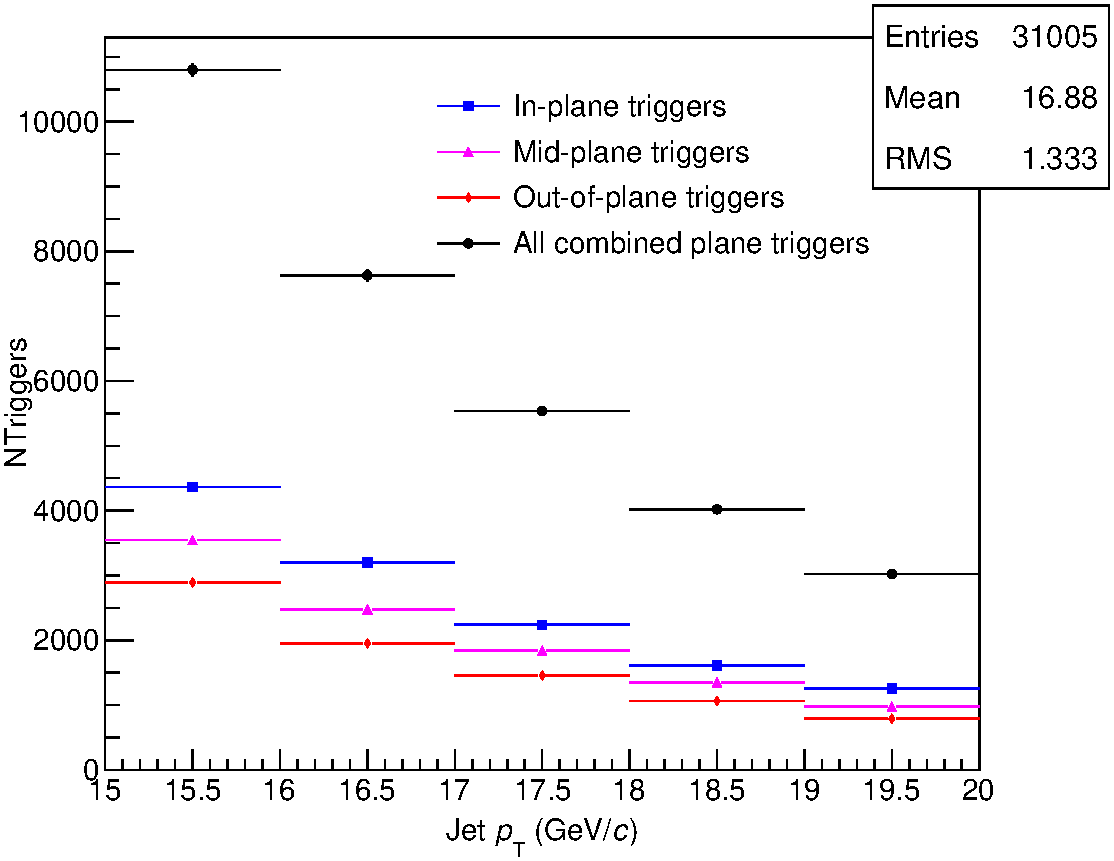
\includegraphics[width=\linewidth]{JHC/NTrig_J15-20_C20-50_Zcut24.pdf} &
		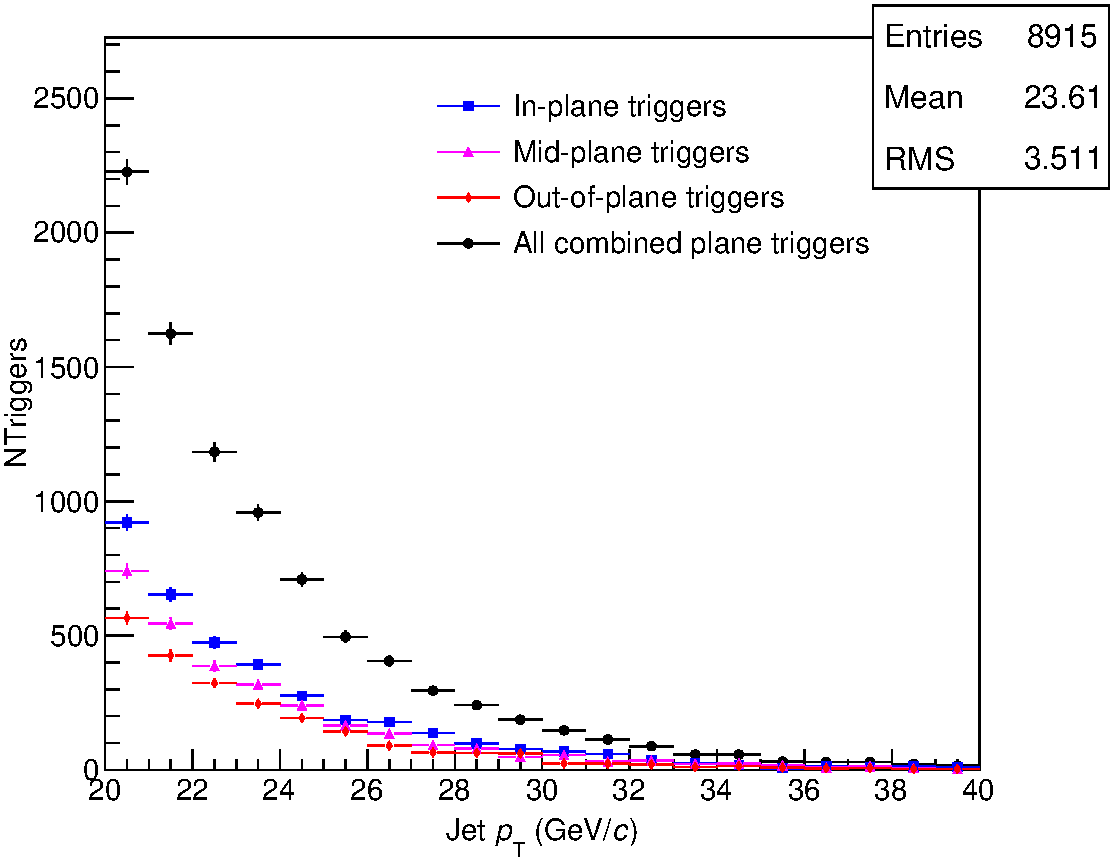
\includegraphics[width=\linewidth]{JHC/NTrig_J20-40_C20-50_Zcut24.pdf} \\
	\end{tabularx}
	\caption[Number of trigger jets for each orientation relative to the event plane]{Number of trigger jets as a function of the reconstructed \Pt{jet} for \pttrigrange{15}{20} (left) and \pttrigrange{20}{40} (right) full jets in 20--50\% central \AuAu collisions, for in-plane (blue), mid-plane (magenta) and out-of-plane (red) jets and all orientations combined (black).}
	\label{fig:NTrig}
\end{figure}

No event-by-event subtraction of the underlying event, $\rho A_{\rm jet}$, is applied to the jet momenta: with 2~\GeVc constituents, too few background \kt jets are found in an event to estimate $\rho$ reliably, and the remaining background contribution is small.
%
The residual background and its dependence on the jet orientation relative to the event plane are instead accounted for by the jet-energy-shift correction described in Sec.~\ref{sect:SysUnc}.
%
The hard-core and trigger-tower requirements select jets that fragmented hard and lost little energy, which favors jets produced close to the surface of the medium and heading outward.
%
This \emph{surface bias} of the trigger jet increases, on average, the path length of the recoiling away-side jet through the medium.

\subsection{Jet-hadron correlation} \label{sect:Correlations}
The measurement of the correlation function (distribution of charged hadrons relative to reconstructed jets) described in Eq.~\ref{Eq:JHCorrIntro} requires several corrections.  The correlation function is measured in pseudorapidity (\deta) and azimuth (\dphi) as: 

\begin{equation}
	\frac{1}{N_{\rm trig}} \frac{d^2N_{\rm assoc,jet}}{d\dphi d\deta} = \frac{1}{N_{\rm trig}} \frac{1}{\epsilon(\Pt{assoc}, \eta_{\rm assoc})} \frac{1}{a(\Pt{assoc}, \text{\dphi}, \text{\deta})}\left(\frac{d^2 N^{\rm meas}_{\rm assoc,jet}}{d\dphi d\deta} - \frac{d^2 N^{\rm bkgd}_{\rm assoc,jet}}{d\dphi d\deta}\right) .
	\label{Eqtn:CorrFunction}
\end{equation}

\begin{sidewaysfigure}
	\centering
	\begin{tabularx}{\textwidth}{XXX@{\hskip 0.5cm}XXX}
		%\hline
		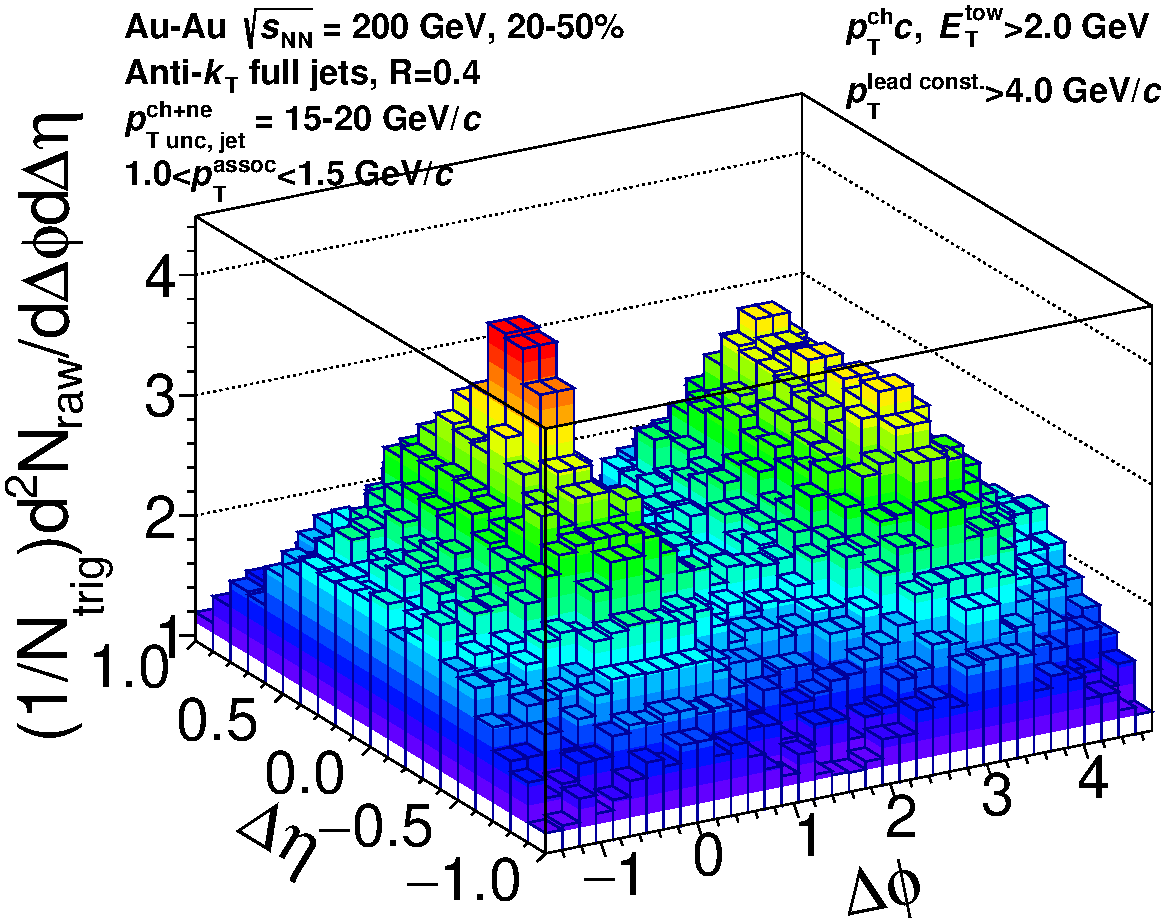
\includegraphics[width=\linewidth]{JHC/J15-20_C20-50_raw2D_sig_in_Ass1.0-1.5_Zcut24.pdf} & 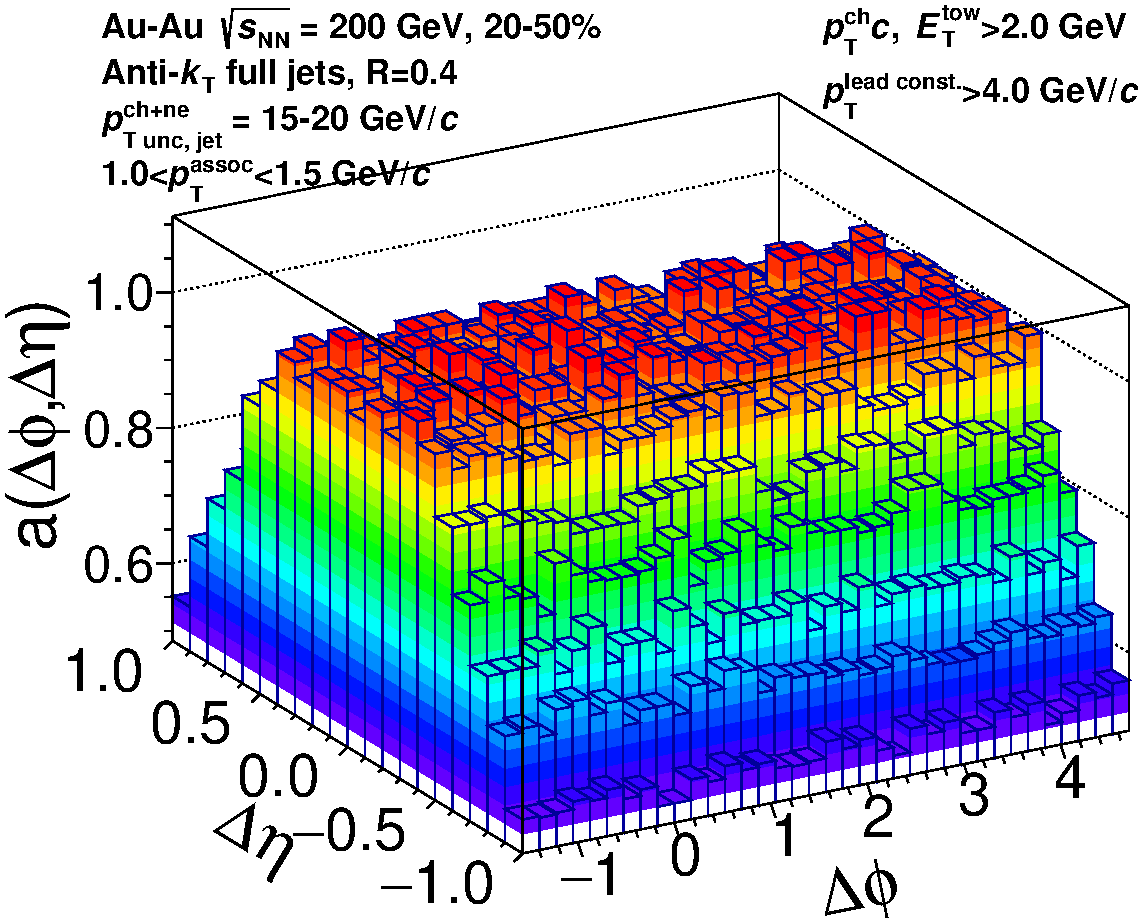
\includegraphics[width=\linewidth]{JHC/J15-20_C20-50_raw2D_mix_in_Ass1.0-1.5_Zcut24.pdf} & 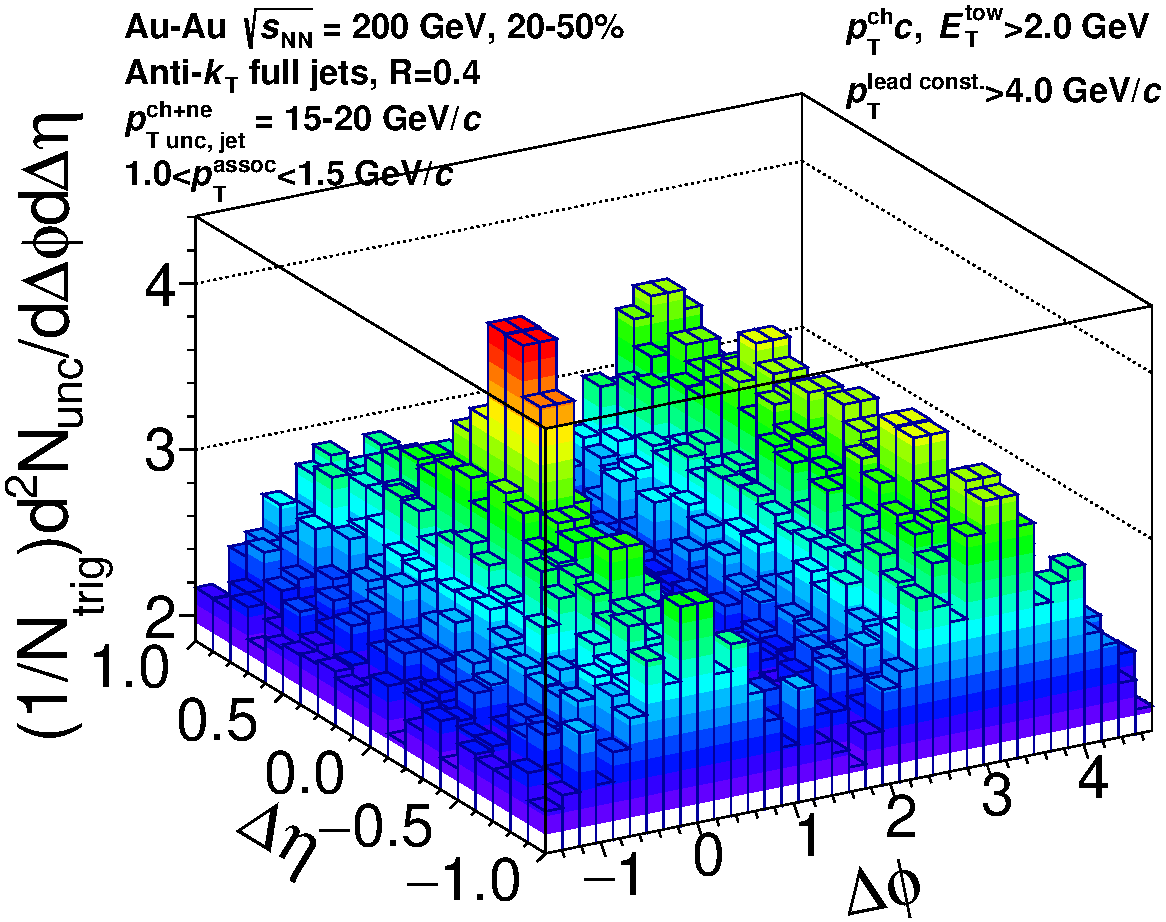
\includegraphics[width=\linewidth]{JHC/J15-20_C20-50_raw2D_ratio_in_Ass1.0-1.5_Zcut24.pdf} &
		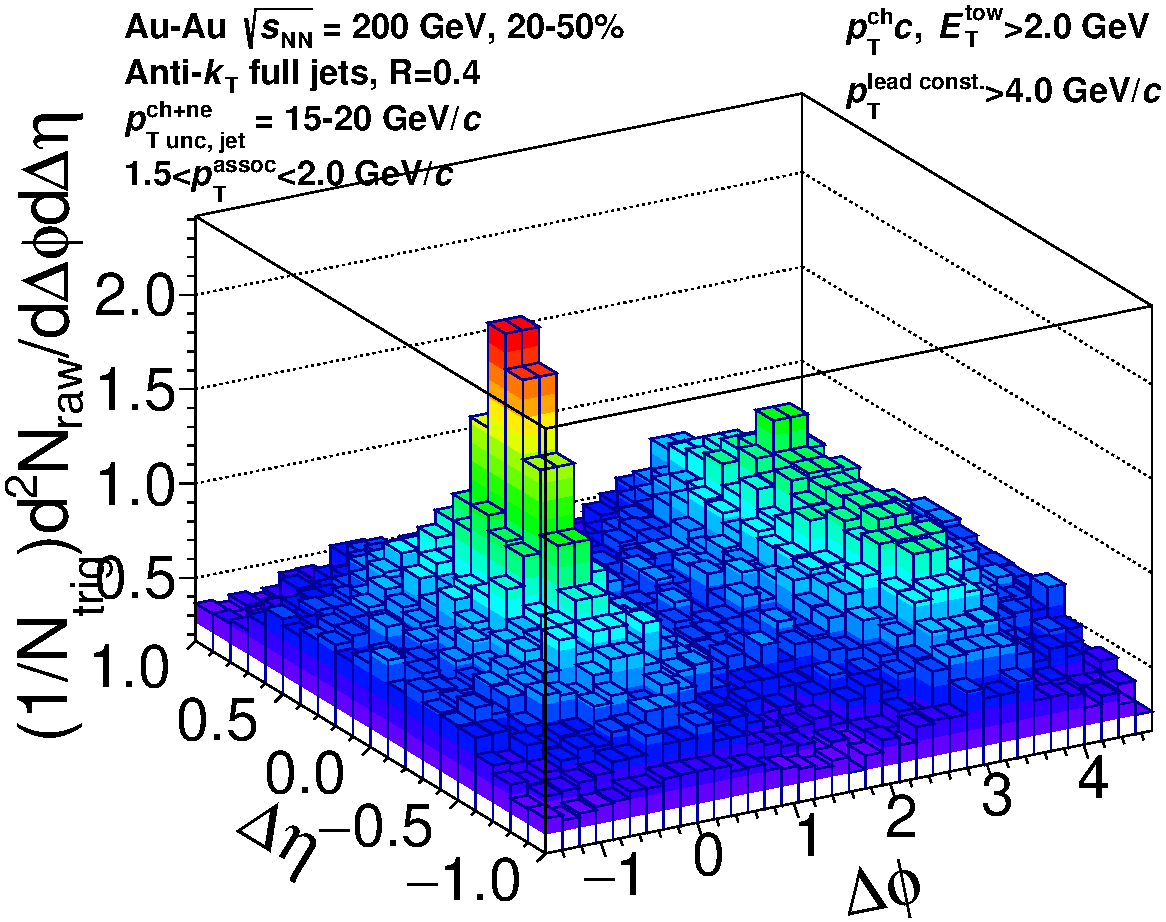
\includegraphics[width=\linewidth]{JHC/J15-20_C20-50_raw2D_sig_in_Ass1.5-2.0_Zcut24.pdf} & 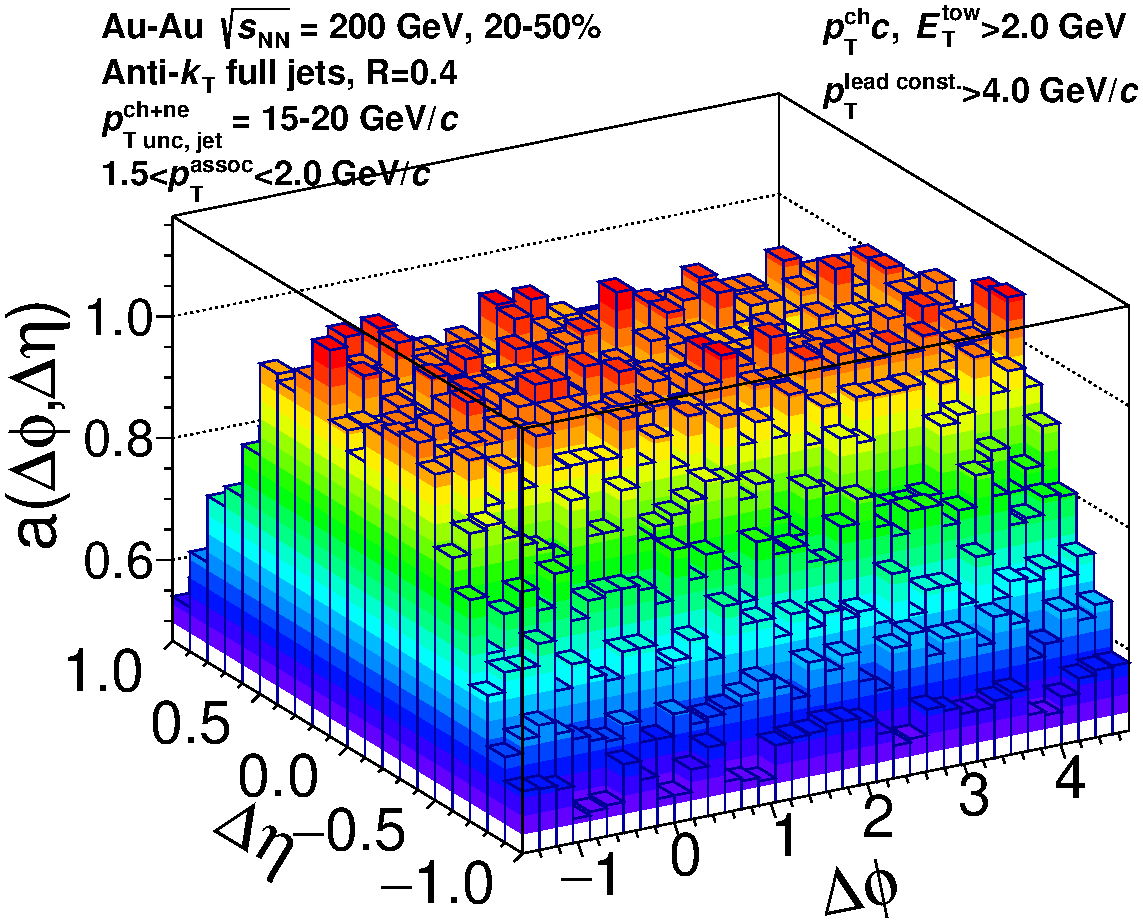
\includegraphics[width=\linewidth]{JHC/J15-20_C20-50_raw2D_mix_in_Ass1.5-2.0_Zcut24.pdf} & 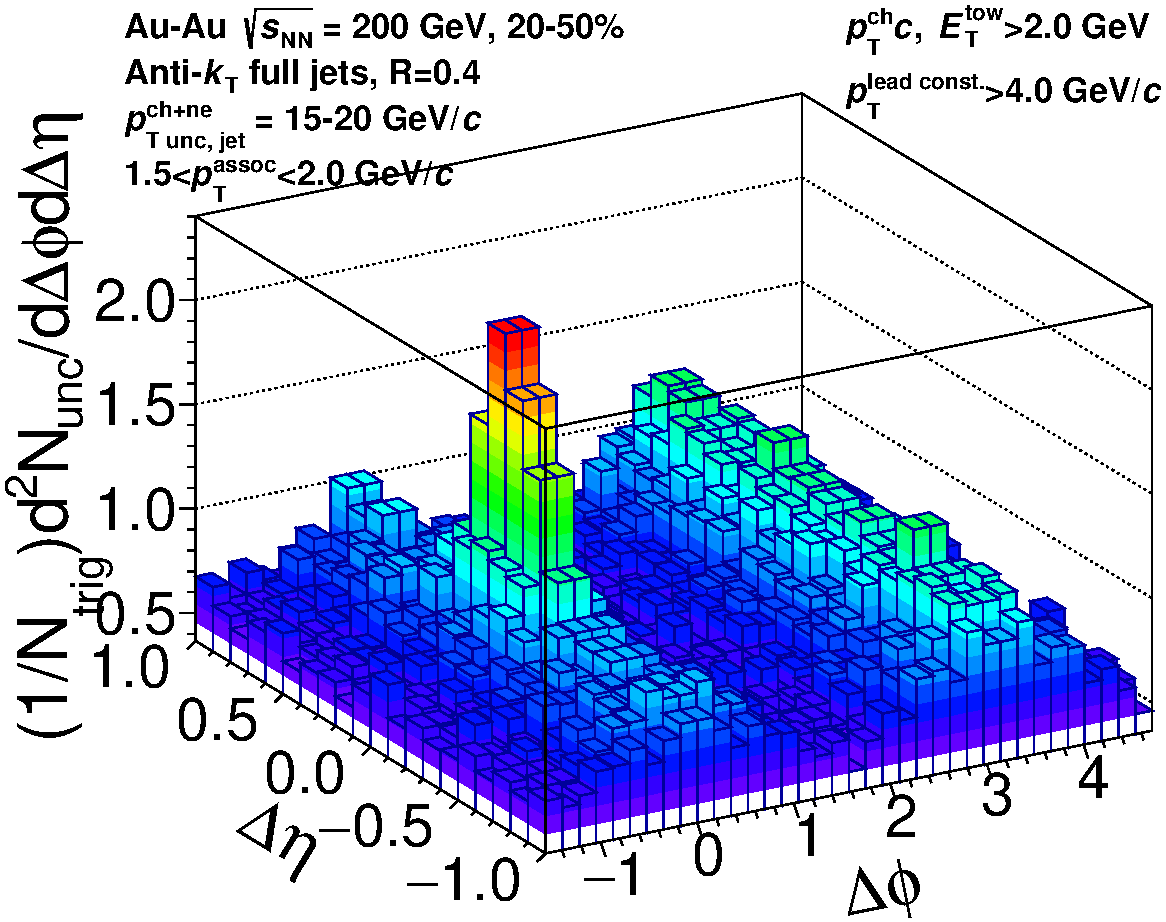
\includegraphics[width=\linewidth]{JHC/J15-20_C20-50_raw2D_ratio_in_Ass1.5-2.0_Zcut24.pdf} \\
		\multicolumn{3}{c}{(a)}&\multicolumn{3}{c}{(b)}\\
		\multicolumn{6}{c}{}\\
		%\hline
		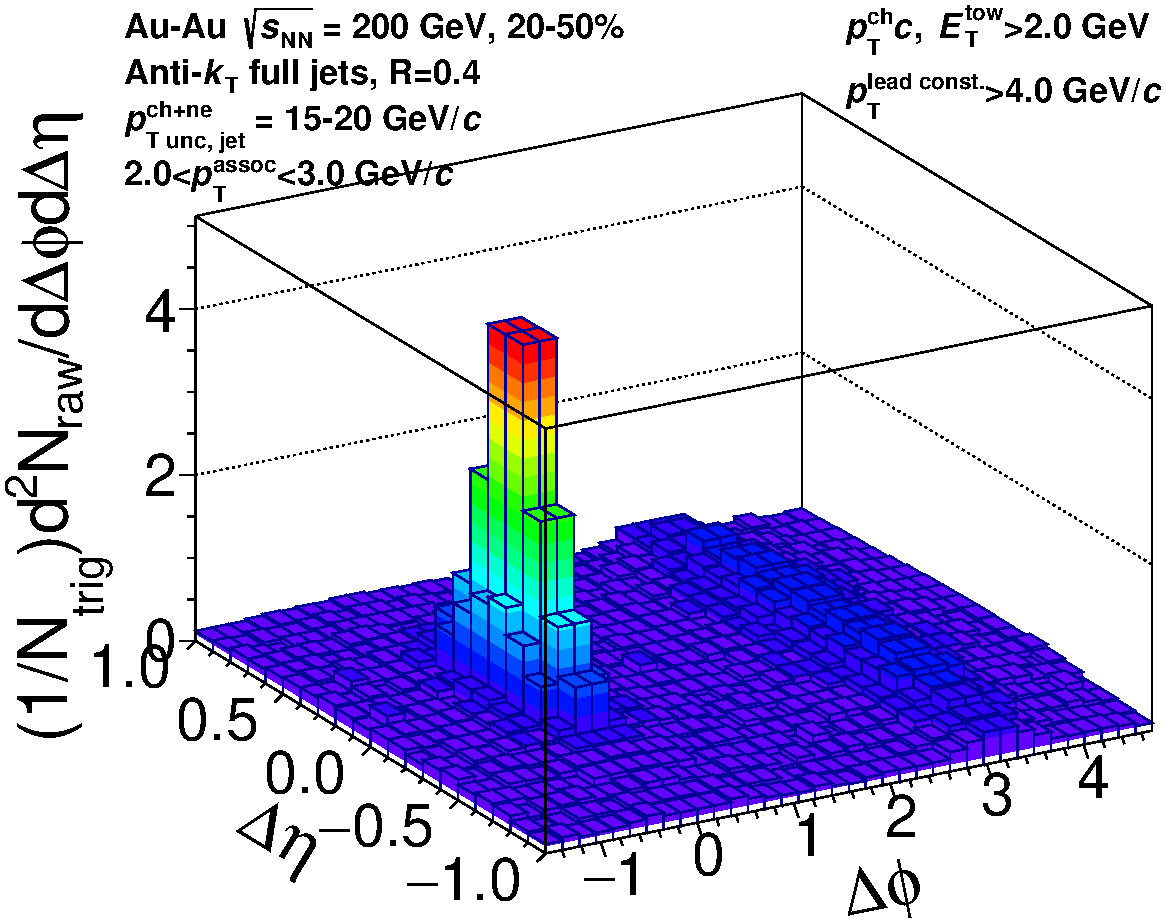
\includegraphics[width=\linewidth]{JHC/J15-20_C20-50_raw2D_sig_in_Ass2.0-3.0_Zcut24.pdf} & 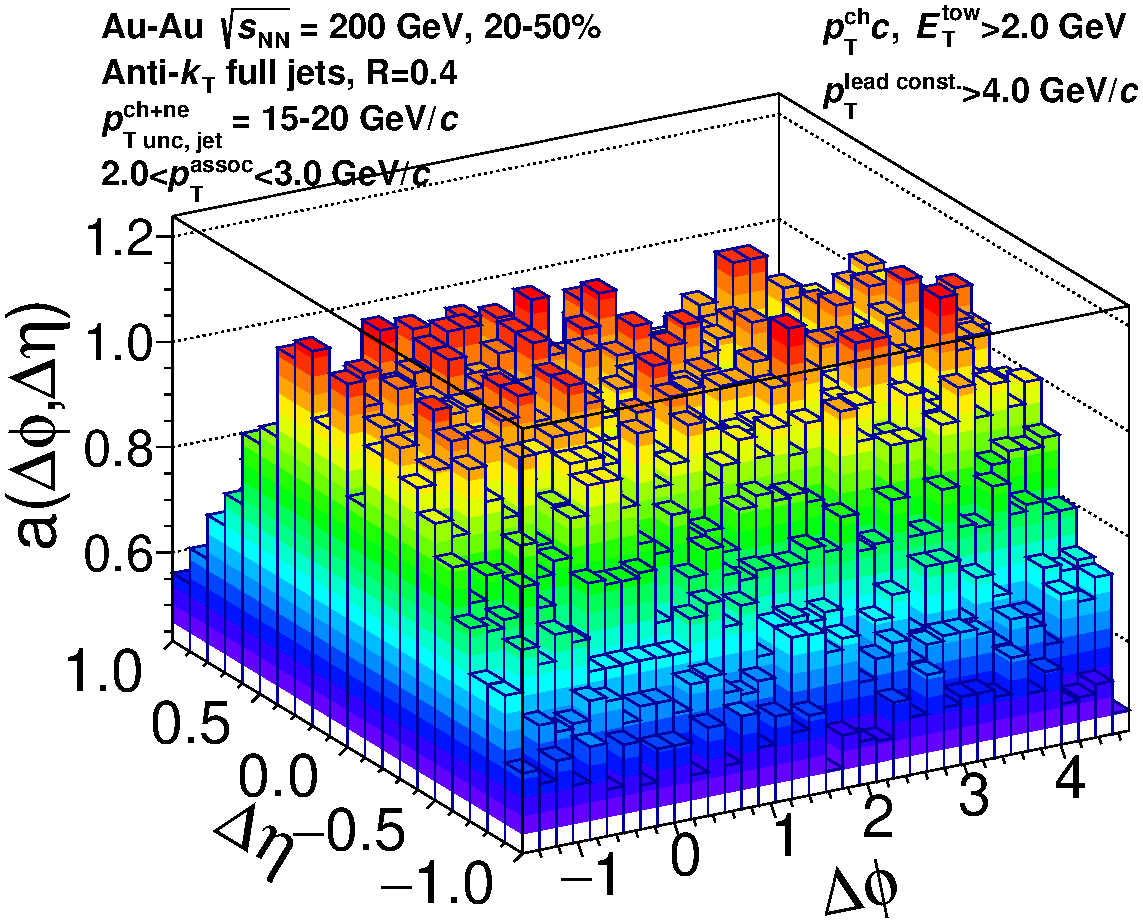
\includegraphics[width=\linewidth]{JHC/J15-20_C20-50_raw2D_mix_in_Ass2.0-3.0_Zcut24.pdf} & 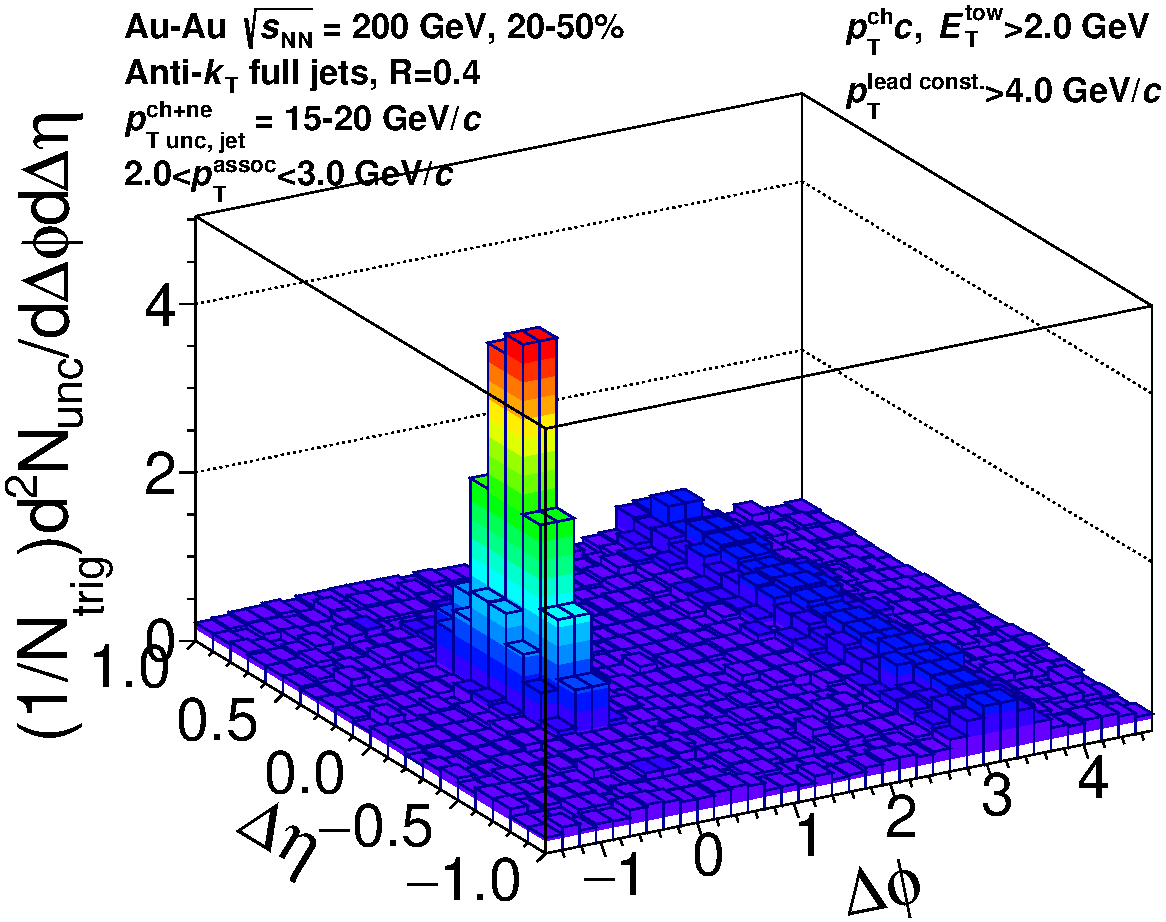
\includegraphics[width=\linewidth]{JHC/J15-20_C20-50_raw2D_ratio_in_Ass2.0-3.0_Zcut24.pdf} &
		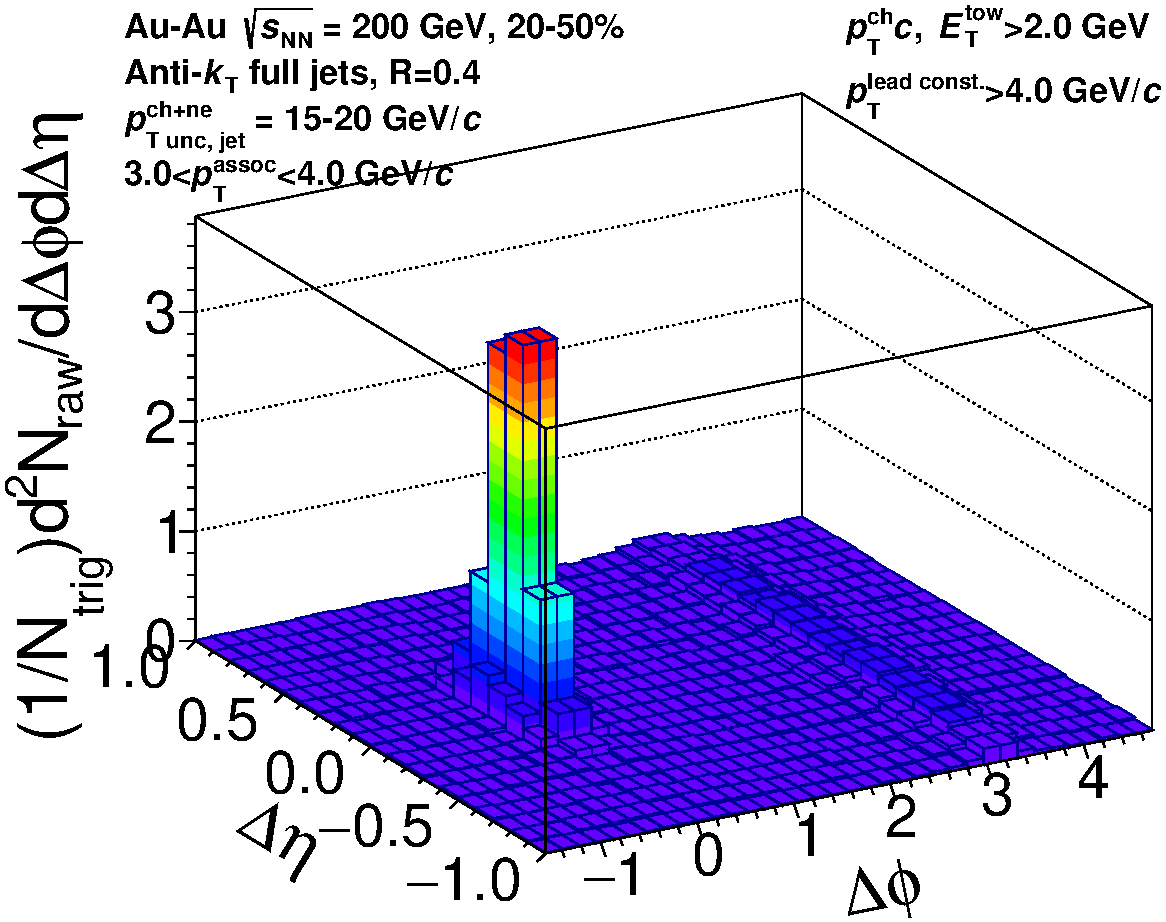
\includegraphics[width=\linewidth]{JHC/J15-20_C20-50_raw2D_sig_in_Ass3.0-4.0_Zcut24.pdf} & 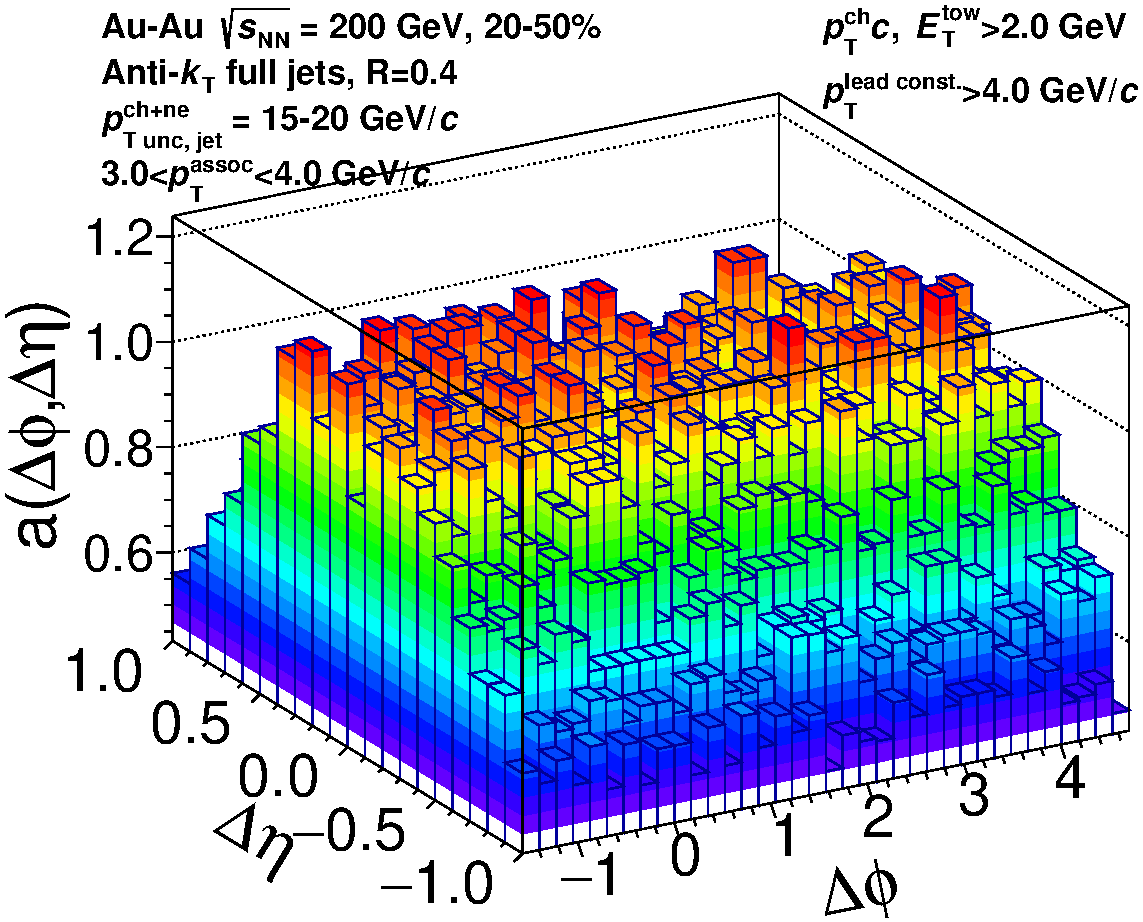
\includegraphics[width=\linewidth]{JHC/J15-20_C20-50_raw2D_mix_in_Ass3.0-4.0_Zcut24.pdf} & 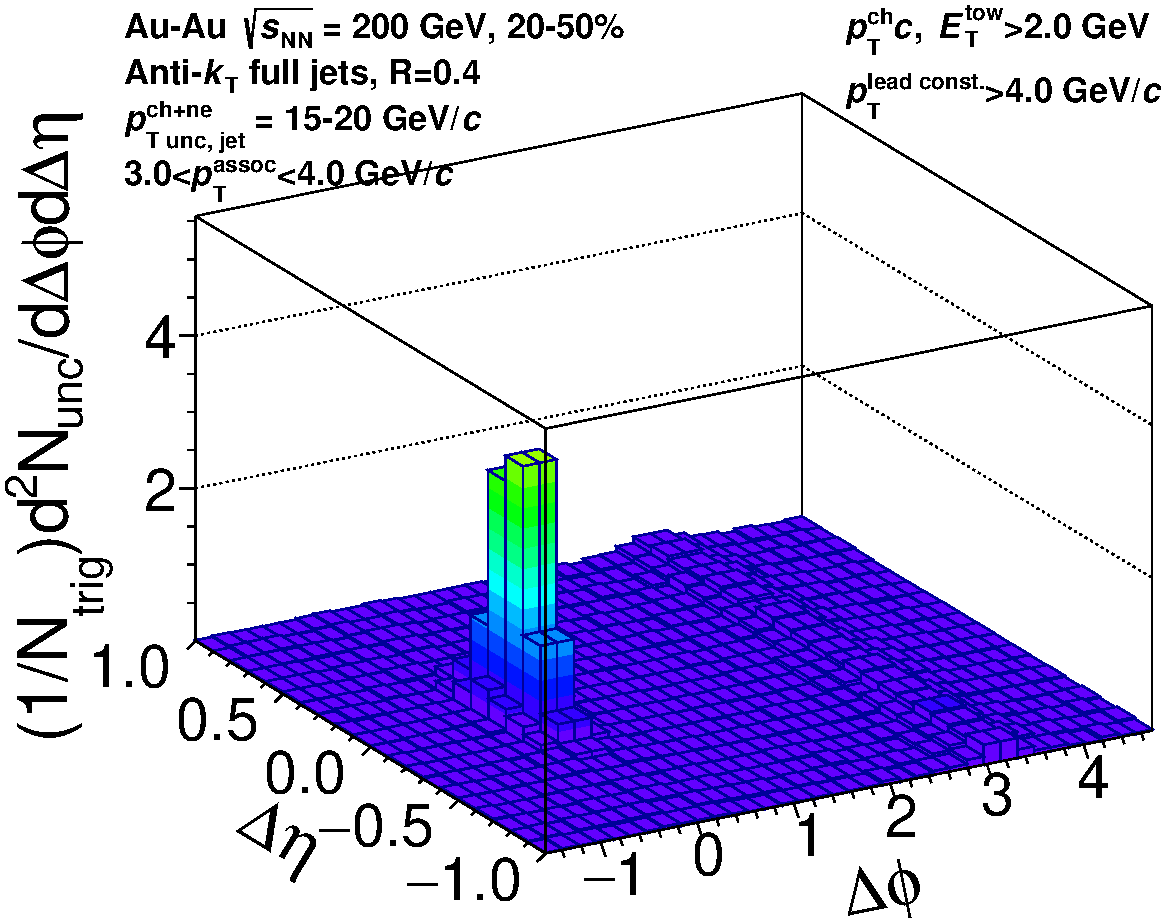
\includegraphics[width=\linewidth]{JHC/J15-20_C20-50_raw2D_ratio_in_Ass3.0-4.0_Zcut24.pdf} \\
		\multicolumn{3}{c}{(c)}&\multicolumn{3}{c}{(d)}\\
		\multicolumn{6}{c}{}\\
		%\hline
		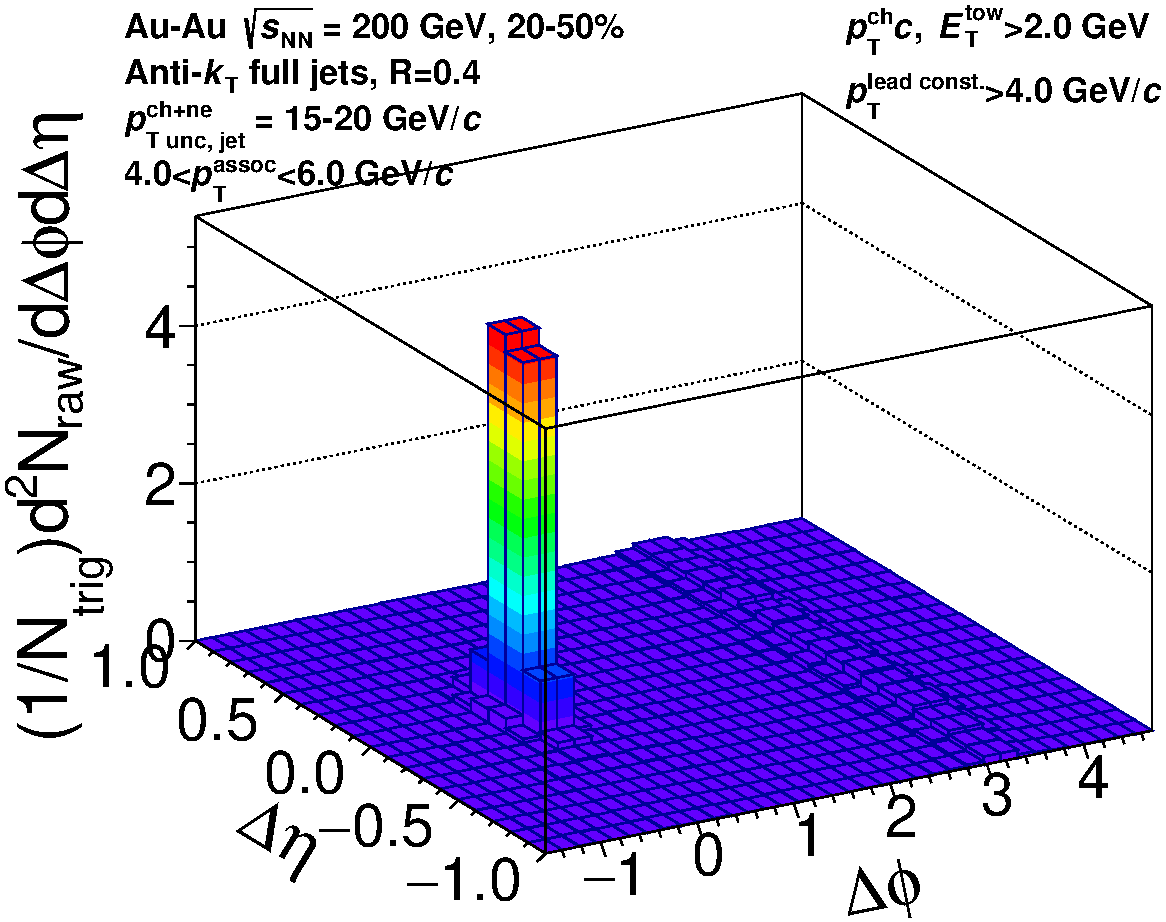
\includegraphics[width=\linewidth]{JHC/J15-20_C20-50_raw2D_sig_in_Ass4.0-6.0_Zcut24.pdf} & 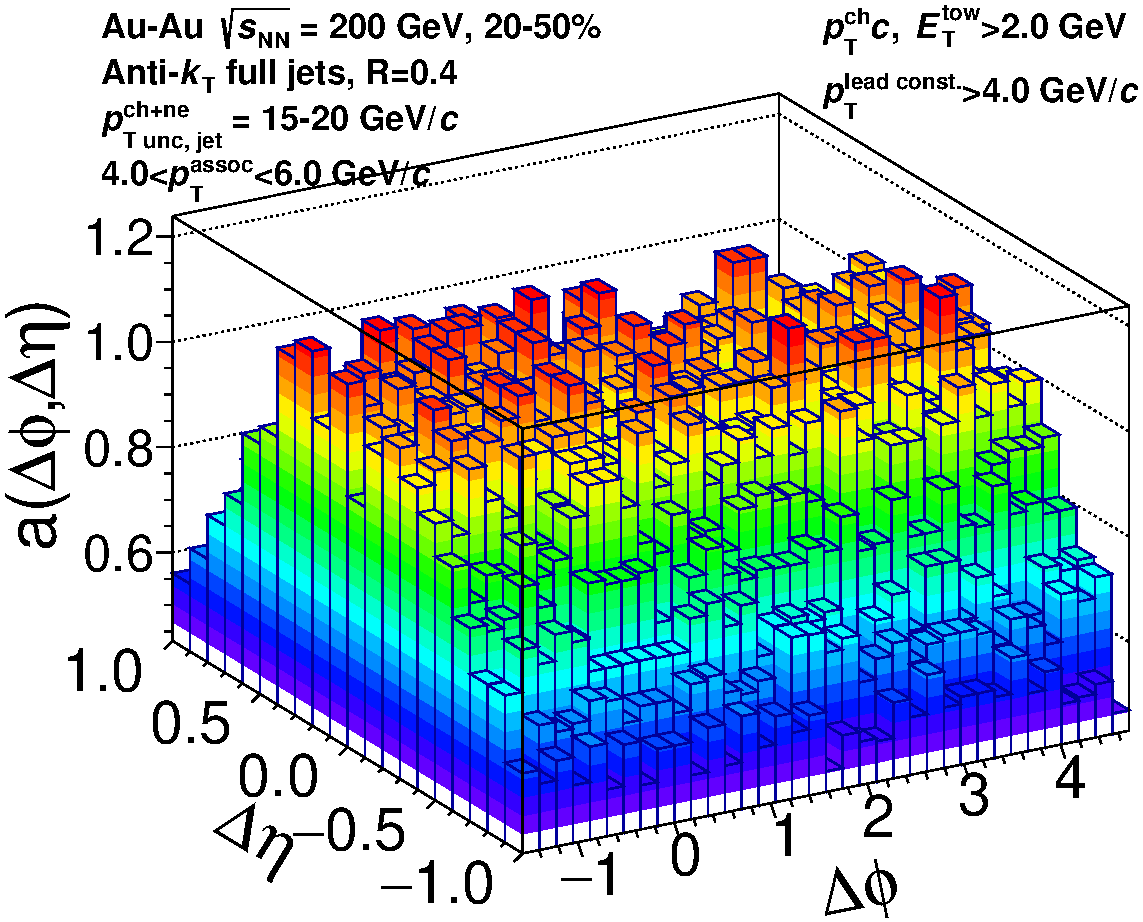
\includegraphics[width=\linewidth]{JHC/J15-20_C20-50_raw2D_mix_in_Ass4.0-6.0_Zcut24.pdf} & 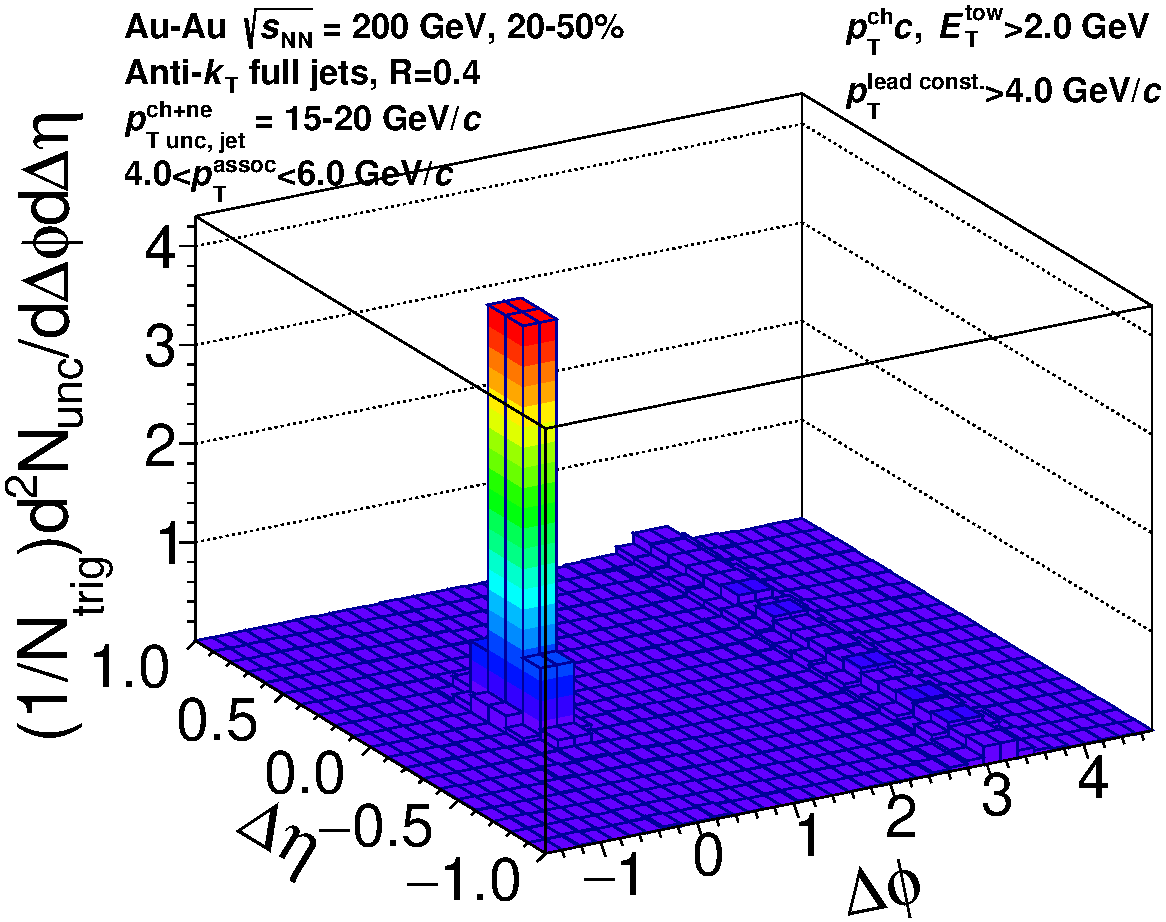
\includegraphics[width=\linewidth]{JHC/J15-20_C20-50_raw2D_ratio_in_Ass4.0-6.0_Zcut24.pdf} &
		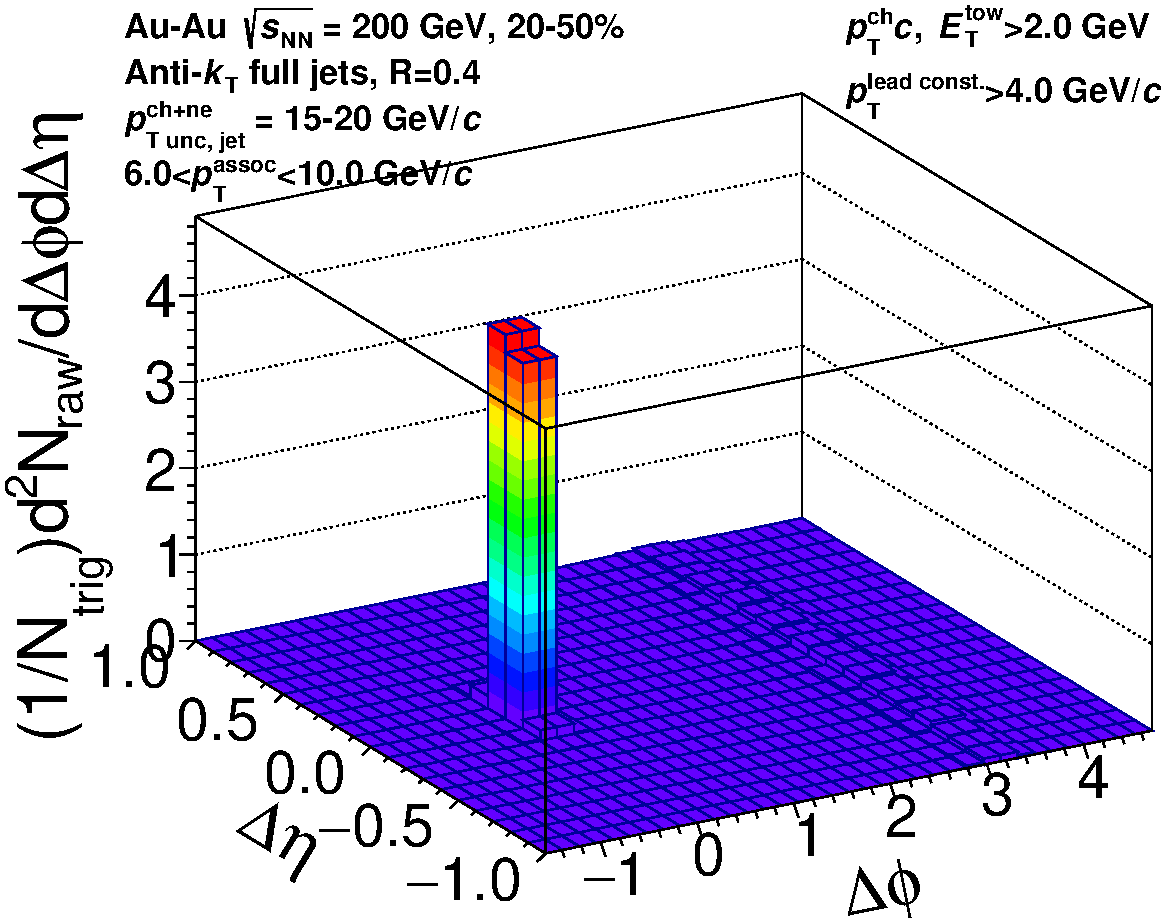
\includegraphics[width=\linewidth]{JHC/J15-20_C20-50_raw2D_sig_in_Ass6.0-10.0_Zcut24.pdf} & 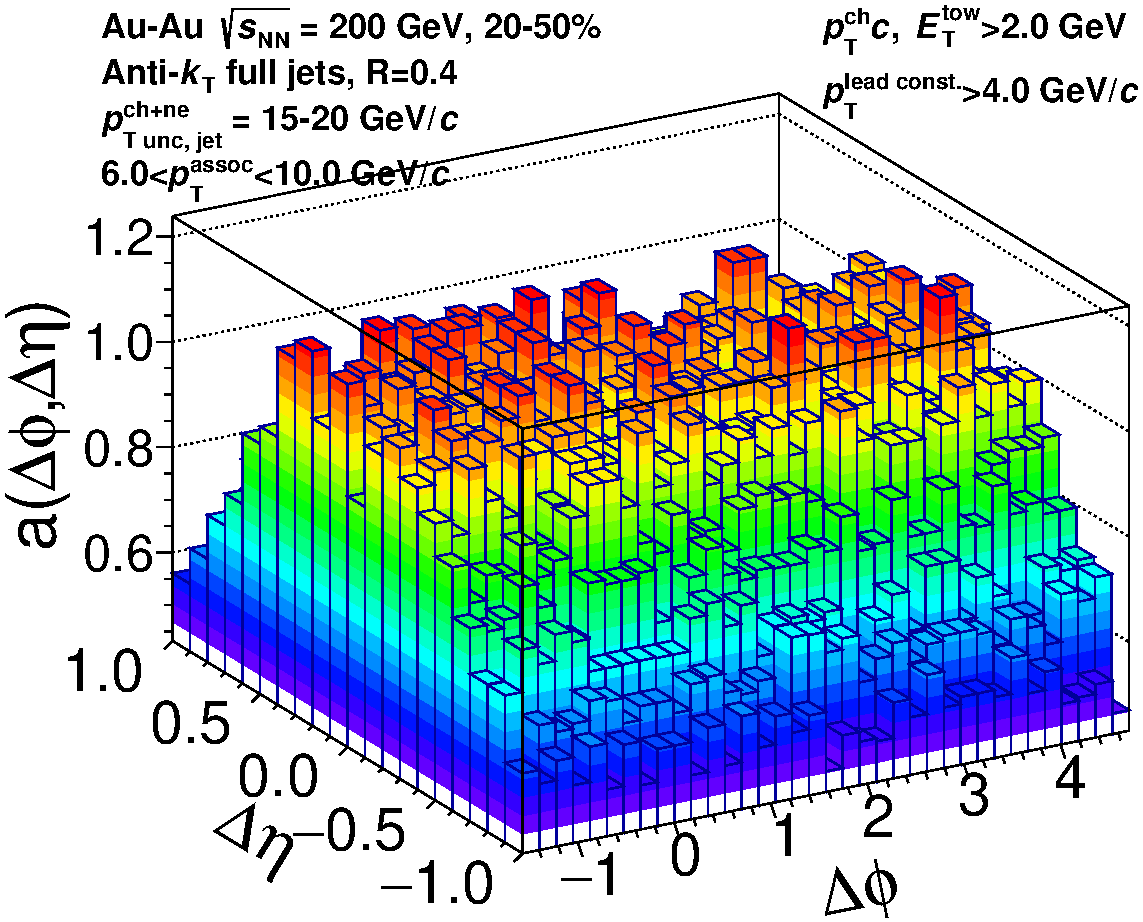
\includegraphics[width=\linewidth]{JHC/J15-20_C20-50_raw2D_mix_in_Ass6.0-10.0_Zcut24.pdf} & 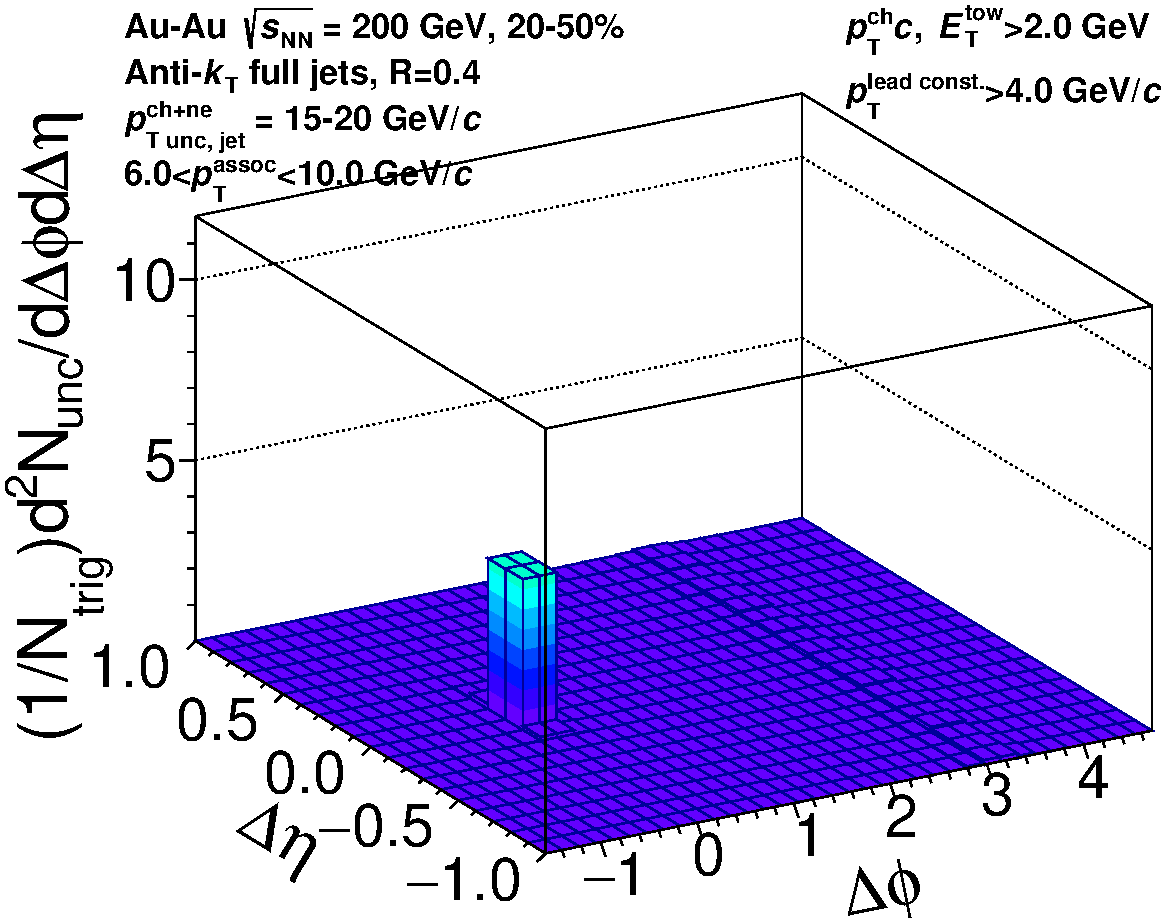
\includegraphics[width=\linewidth]{JHC/J15-20_C20-50_raw2D_ratio_in_Ass6.0-10.0_Zcut24.pdf}\\
		\multicolumn{3}{c}{(e)}&\multicolumn{3}{c}{(f)}\\
		%\hline
	\end{tabularx}
%		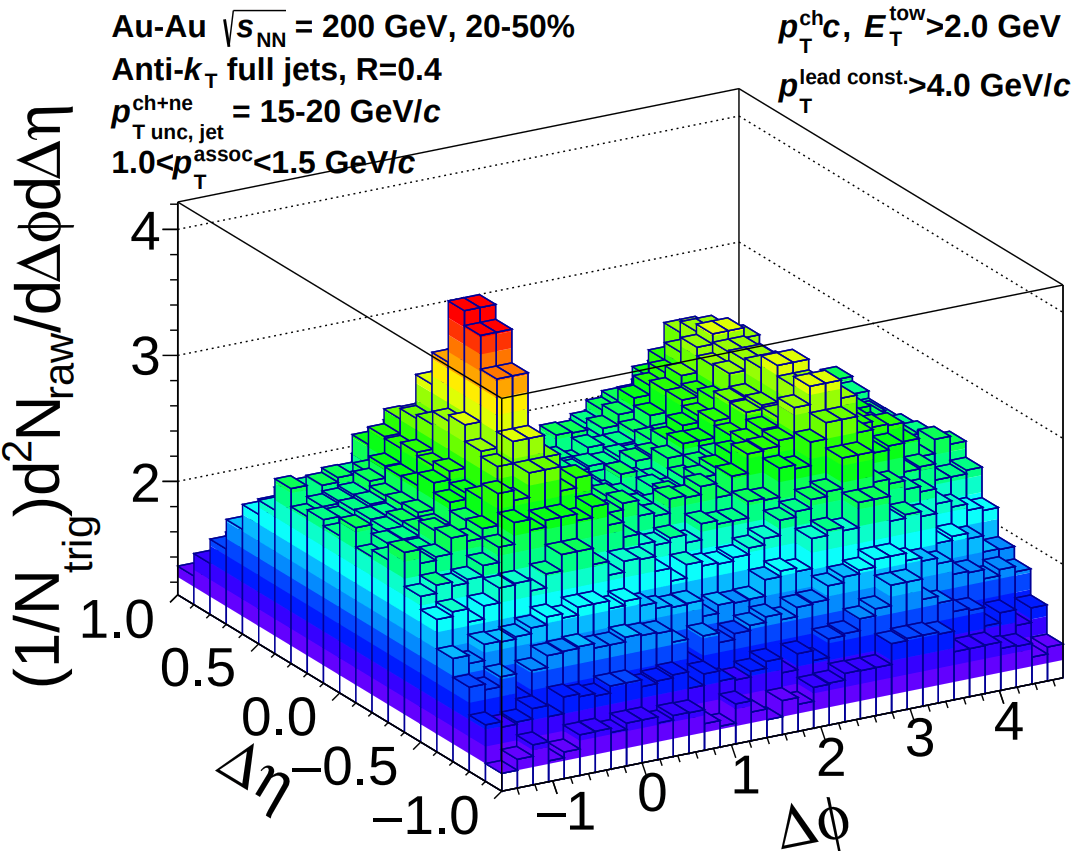
\includegraphics[width=0.49\linewidth]{figures/jhcorr_jpt1520}
%	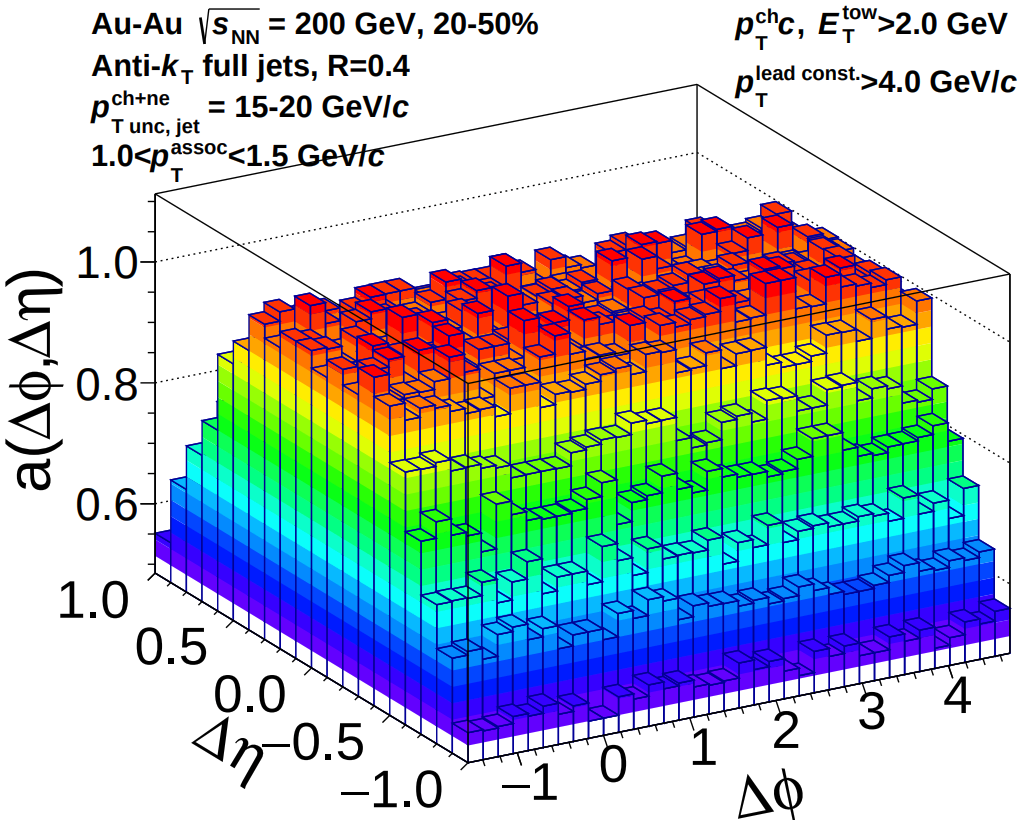
\includegraphics[width=0.49\linewidth]{figures/ajhcorr_jpt1520}
	\caption[Raw, mixed-event and acceptance-corrected jet-hadron correlations for 15--20~GeV/\(c\) jets]{Two-dimensional jet-hadron correlations in \dphi and \deta for in-plane \pttrigrange{15}{20} jets in 20--50\% central \AuAu collisions, for the associated-hadron momenta (a) \ptassocrange{1.0}{1.5}, (b) \ptassocrange{1.5}{2.0}, (c) \ptassocrange{2.0}{3.0}, (d) \ptassocrange{3.0}{4.0}, (e) \ptassocrange{4.0}{6.0} and (f) \ptassocrange{6.0}{10.0}. Each group shows, from left to right, the raw same-event distribution per trigger jet, the normalized mixed-event pair acceptance $a(\dphi, \deta)$, whose trapezoidal shape in \(\Delta\eta = \eta_\mathrm{jet} - \eta_\mathrm{assoc}\) follows from \(|\eta_\mathrm{assoc}| < 1.0 \) and \(|\eta_\mathrm{jet}| < 0.6 \), and the acceptance-corrected correlation function, which still contains the combinatorial background.}
	\label{fig:jhcorrjpt1520}
\end{sidewaysfigure}

%\noindent where and acceptance, $a(\dphi, \deta)$ is the acceptance correction for track pairs, $N_{meas}$ is the measured number of associated particles, and $N_{bkgd}$ is the number of associated particles from the background.  The single-track reconstruction efficiency and acceptance only account for the reconstruction of associated particles.
%\begin{equation}
%   C(\dphi, \deta)= \frac{  \frac{d^2 N^{same}_{pair}}{d\dphi 
		%   d \deta}} {  \frac{d^2 N^{mixed}_{pair}}{d \dphi d \deta}}
%   \label{Eqn:correlationfnc}
%\end{equation}

%and express our associated per trigger yield by:

%\begin{equation}
%  \frac{d^2 N}{d\dphi d\deta}(\dphi,\deta,\Delta\Psi_{RP,2}) = \frac{1}{N_{trig}} %\frac{dN_{assoc}}{d\dphi d\deta}
%  \label{Eqn:correlationfncPerTrig}
%\end{equation}

Here, $N_{\rm assoc, jet}$ gives the number of pairs of trigger jets and the associated hadrons, $N^{\rm meas}_{\rm assoc,jet}$ and $N^{\rm bkgd}_{\rm assoc,jet}$ are the number of pairs measured and the pair characterized as background respectively. The single-track reconstruction efficiency is $\epsilon(\Pt{assoc}, \eta_{\rm assoc})$\footnote{Acceptance effects such as gaps between sector boundaries are included in this correction; however, $\epsilon(\Pt{assoc}, \eta_{\rm assoc})$ is referred to as an efficiency correction in order to distinguish it from $a(\Pt{assoc}, \text{\dphi}, \text{\deta})$.}.  The pair acceptance, $a(\Pt{assoc}, \text{\dphi}, \text{\deta})$, is calculated from the raw pairs measured between a trigger jet and the charged hadrons from mixed events.  %The background correction $N_{\rm bkgd}$ is described in Sec.~\ref{sect:CorrBkgd}.

The correlations are determined in bins of centrality, reconstructed trigger-jet transverse momentum (\Pt{jet}), associated-hadron transverse momentum (\Pt{assoc}), and bins of the trigger jet relative to the event plane (in, mid, out, all combined angles) defined in Eq.~\ref{Eq:EPbins}.  Fig.~\ref{fig:jhcorrjpt1520} shows, for in-plane \pttrigrange{15}{20} jets, how the raw same-event distributions are turned into acceptance-corrected correlation functions by the mixed-event correction described below.  The corrected correlation functions contain a large combinatorial background ($N^{\rm bkgd}_{\rm assoc,jet}$), which must be subtracted.  This subtraction procedure is described in Sec.~\ref{sect:CorrBkgd}.

%The acceptance correction is applied in \dphi and \deta before further analysis and background subtraction.  Figure shows an example of the raw correlations from same events pairs before applying a mixed event correction for the efficiency and acceptance of the BEMC.  A plateau structure can be seen due to the finite acceptance of track pairs.


%=============================================================
%=============================================================
\subsubsection{Pair-acceptance correction from mixed events}
\label{sect:MixedEvents}
% Mixed events should not contain physics correlations, but information of the acceptance and efficiency of single event pairs.

The pair-acceptance correction, $1 / a(\Pt{assoc}, \text{\dphi}, \text{\deta})$, accounts for the detector and tracking inefficiencies, and is found by correlating jets from HT-triggered events with associated hadrons from MB events of the same event class. %(centrality, primary vertex position in the z-direction).  
%
In addition to providing the acceptance correction, the mixed-event procedure will also help remove the trivial correlation due to an $\eta$ dependence in the single-particle track distributions~\cite{PhysRevC.101.064901}.  
%
Taking the ratio of the same-event pairs to the mixed-event pairs removes the detector effects of acceptance and efficiency.  
%
The pair acceptance will serve as the dominant effect, given that there is little $\eta$ dependence in both the tracks and jets across the acceptance range of this analysis.
%
Since the trigger jets are restricted to $|\eta_\mathrm{jet}| < 0.6$ and the associated hadrons to $|\eta_\mathrm{assoc}| < 1.0$, the number of possible pairs is constant for $|\deta| < 0.4$ and falls linearly to zero at $|\deta| = 1.6$, which gives the pair acceptance its trapezoidal shape in \deta, illustrated with a toy model in Fig.~\ref{fig:ToyMixedEvent} and visible in the measured mixed-event distributions of Fig.~\ref{fig:jhcorrjpt1520}.
%
Because the trigger jet and the associated hadrons of a mixed pair come from different events, they are correlated only through this acceptance.

\begin{figure}[!htbp]
	\centering
	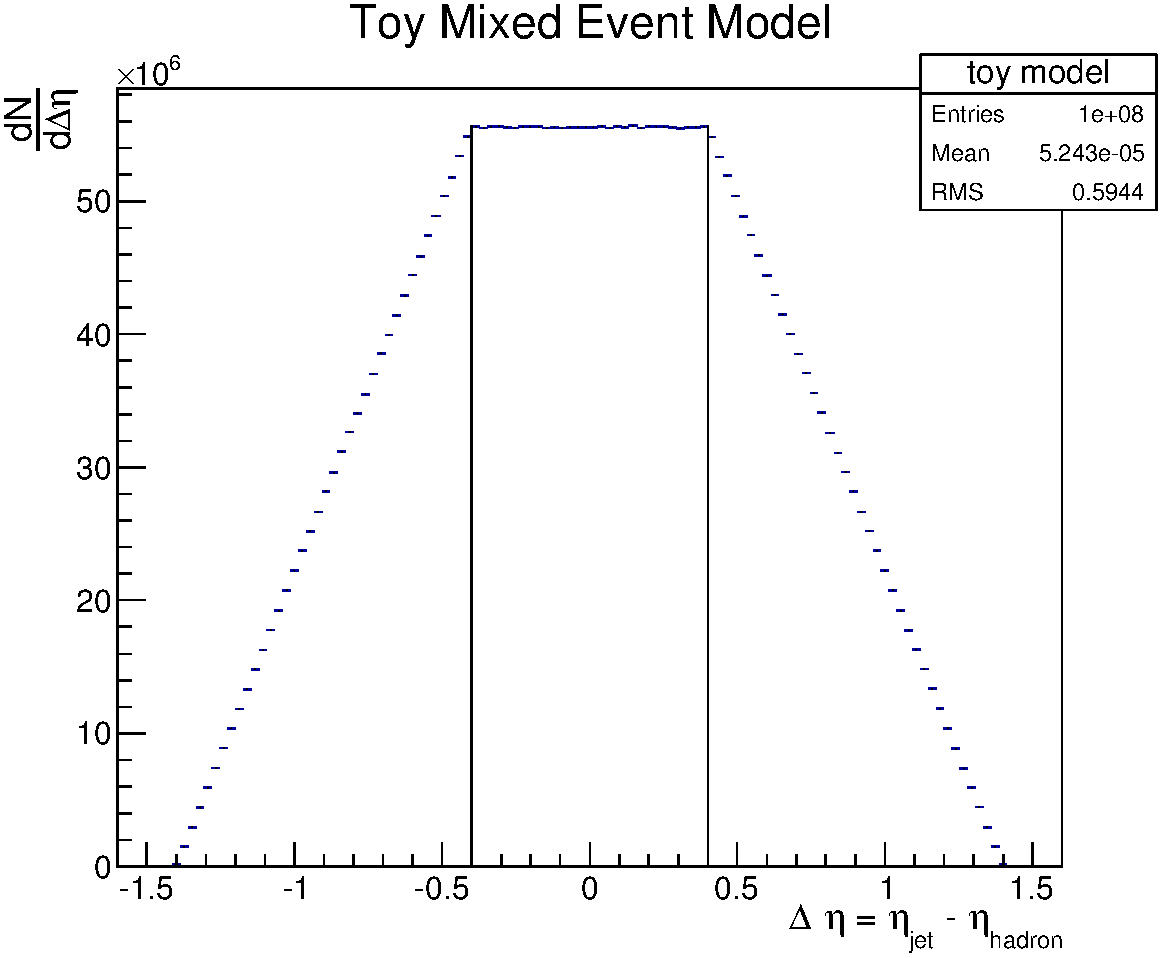
\includegraphics[width=0.6\linewidth]{JHC/ToyMixedEventModel-eps-converted-to.pdf}
	\caption[Toy model of the pair acceptance in \(\Delta\eta\)]{Toy model of the pair acceptance in $\deta = \eta_\mathrm{jet} - \eta_\mathrm{hadron}$ for uncorrelated trigger jets and hadrons, each uniformly distributed in pseudorapidity (here $|\eta_\mathrm{jet}| < 0.5$ and $|\eta_\mathrm{hadron}| < 0.9$). The number of pairs is constant where the smaller acceptance is fully contained in the larger one and falls linearly to zero at the largest possible separation. The analysis uses the plateau region $|\deta| < 0.4$ to normalize the measured mixed-event distributions.}
	\label{fig:ToyMixedEvent}
\end{figure}


%To increase the sampling size of mixed events used for the acceptance correction, both MB30 and MB5 triggered events are used for event mixing.  After re-weighting the reference multiplicity distributions to correct for the VPD trigger inefficiency, MB5 events are added with an additional weight factor such that they are normalized to MB30 events in a 2-dimensional fashion to account for VPD resolution differences across centrality and the online VPD vertex cut which had a negative $v_z$ offset.  Additional details can be found in Ref.~\cite{PhysRevC.99.034908}.  

The event mixing follows Ref.~\cite{PhysRevC.96.024905}. The MB events are kept in pools binned in 10\% centrality and 4-cm $v_z$ intervals, each holding up to 25\,000 tracks; each trigger jet is correlated with the tracks of all events in the pool of its event class, and the mixed-event pairs are weighted by the inverse of the number of mixed events. The acceptance is constructed separately for the 20--30\%, 30--40\%, and 40--50\% centrality classes and then combined.  High-momentum tracks are nearly straight, so the detector acceptance does not change significantly at high-\Pt{assoc}, and thus all associated momentum bins greater than 2.0 \GeVc are combined to increase statistics.  There is no difference in efficiency and acceptance within uncertainties for different orientations of the jet relative to the event plane, and therefore the same correction $a(\Pt{assoc}, \text{\dphi}, \text{\deta})$ is applied for all angles relative to the event plane.  The acceptance $a(\Pt{assoc}, \text{\dphi}, \text{\deta})$ is normalized to 1 at its maximum, determined using the region of approximately constant acceptance ($|\deta| <$ 0.4).  For each \Pt{assoc} bin, the projection of the flat plateau region (integrated over the region $|\deta| <$ 0.4) was fit with a constant over the whole \dphi range.

\subsubsection{Uncertainties of the pair-acceptance correction}
\label{sect:MixedEventsUnc}
Three uncertainties are associated with the pair-acceptance correction: the normalization of the mixed events, and the shape of the correction in \dphi and in \deta that results from its dependence on the vertex position.
%
The uncertainties of the fits of the plateau were used for the systematic uncertainty on the mixed-event normalization, which is added in quadrature and reported as the scale uncertainty.  This systematic uncertainty is under 1\% (1.25\%) in all \Pt{assoc} bins used for the reported results of jets with  \pttrigrange{15}{20} and  \pttrigrange{20}{40}.

A shape uncertainty in \dphi due to the \zvtx binning, similar to that in \deta, could lead to an additional shape uncertainty in the correlation functions.  To test for this, the ratio of the 1D \dphi projection with the nominal \zvtx binning and the binning described above was calculated for each \Pt{jet}, \Pt{assoc}, and centrality bin.  The variations about 1.0 are smaller than the statistical errors associated with the points.  This uncertainty was therefore considered negligible.

There is an additional shape uncertainty associated with the application of the acceptance correction due to slight changes in the correlation function at large \deta in the acceptance with $v_z$ position.  The background level is determined from the level of the correlation function at large \deta, leading to a scale uncertainty in the background subtraction dependent on \Pt{assoc}.  This uncertainty is from the differences between the nominal (z-integrated) and the z-vertex method (z-binned) for correcting the mixed events on the level of the background in the $0.6 < \deta < 1.2$ range, and signal plus background, in the $|\deta| < 0.6$ range.  The large \deta region is used to determine the background so any uncertainties in the level of the correlation function in this region lead to an uncertainty in the level of the background in the signal region.  This is expressed as an additional scale band on the final results.

In the nominal (z-integrated) method the same- and mixed-event distributions are summed over all $v_z$ bins before the division, because dividing the sample into 4-cm $v_z$ bins, as would be ideal given the $v_z$ dependence of the acceptance, enlarges the statistical fluctuations of the mixed-event normalization in each bin.
%
In the z-binned method the acceptance correction is instead applied separately in each bin $i$,
%
\begin{equation}
	\frac{1}{N_{\rm trig}} \frac{d^2N_{\rm assoc,jet}}{d\dphi d\deta} = \frac{1}{N_{\rm trig}} \sum_i \frac{1}{\epsilon\, a_i(\dphi, \deta)} \frac{d^2 N_i}{d\dphi d\deta},
	\label{Eqtn:CorrFunctionZbinned}
\end{equation}
%
where $N_i$ and $a_i$ are the same-event pairs and the pair acceptance in $v_z$ bin $i$.
%
For each method, the ratio of the integrals of the correlation function $Y$ over the signal+background ($|\deta| < 0.6$) and background-dominated ($0.6 < |\deta| < 1.2$) regions is computed, and their ratio defines the scale factor
%
\begin{equation}
	\alpha = \frac{\int_\mathrm{sig} Y_\mathrm{nom}\, d\deta \Big/ \int_\mathrm{bkgd} Y_\mathrm{nom}\, d\deta}{\int_\mathrm{sig} Y_{z\mathrm{vtx}}\, d\deta \Big/ \int_\mathrm{bkgd} Y_{z\mathrm{vtx}}\, d\deta}
	\label{Eqtn:alpha}
\end{equation}
%
for each \Pt{assoc} bin.
%
The scale band is obtained by multiplying the correlation function by $\alpha$ and by $2 - \alpha$.
%
This uncertainty is determined by varying the binning of the mixed events in $v_z$ and is correlated for different angles relative to the event plane and for different bins in \Pt{assoc}.  For $\Pt{assoc} >$ 3~\GeVc, this uncertainty is negligible because the background is small.

\subsection{Flow modulation of combinatorial background} \label{sect:CorrBkgd}
The combinatorial background ($N^{\rm bkgd}_{\rm assoc,jet}$) from Eq.~\ref{Eqtn:CorrFunction} can be parametrized for trigger jets restricted to the orientation $\mathfrak{R} = {\text{in/mid/out-of-plane}}$ relative to the event plane as~\cite{Bielcikova:2003ku,Sharma:2015qra}:

\begin{equation}
	\left(\frac{1}{\pi}\frac{dN^{\rm bkgd}_{\rm assoc,jet}}{d\dphi}\right)_\mathfrak{R} = B^\mathfrak{R}\left( 1 + \sum_{n=2}^{\infty} 2 v_{n,\mathrm{assoc}} v^\mathfrak{R}_{n, \mathrm{jet}} \cos(n\dphi)\right)
	\label{Eqtn:JBBBCorrelations},
\end{equation}

\noindent where $v_{n,\mathrm{assoc}}$ and $v^\mathfrak{R}_{n, \mathrm{jet}}$ are the Fourier coefficients of the azimuthal angle distribution (flow coefficients) of background associated particles and trigger jets restricted to the orientation $\mathfrak{R}$ respectively. The factor $B^\mathfrak{R}$ gives the background level amplitude for orientation $\mathfrak{R}$. The trigger jets being restricted to orientation $\mathfrak{R}$ modifies their nominal flow coefficients $v_{n, \mathrm{jet}}$'s into the $v^\mathfrak{R}_{n, \mathrm{jet}}$ from Eq.~\ref{Eqtn:JBBBCorrelations} which are related to each other as ~\cite{Bielcikova:2003ku}:

\begin{equation}
	v^{\mathfrak{R}}_{n, \mathrm{jet}} = 
	\begin{cases}
		\frac{v_{n, \mathrm{jet}}}{\beta^\mathfrak{R}}+ \cos(n\phi_{s}^\mathfrak{R}) \frac{\sin(nc)}{nc}\frac{R_{n}}{\beta^\mathfrak{R}} + &\\
		\frac{1}{\beta^\mathfrak{R}}\sum_{k=2,4,6,..} (v_{(k+n), \mathrm{jet}}+v_{|k-n|, \mathrm{jet}})
		\cos(k\phi_{s}^\mathfrak{R}) \frac{\sin(kc)}{kc}R_{k} & \text{if $n$ is even,}\\
		v_{n, \mathrm{jet}} & \text{if $n$ is odd.}
	\end{cases},
	\label{Eq:vRn}
\end{equation}
where, $\beta^\mathfrak{R}$ is the $\mathfrak{R}$ dependence of $B^\mathfrak{R}$ given by,
\begin{equation}
	B^\mathfrak{R} \propto \beta^\mathfrak{R} = 1 + \sum_{k=2,4,6,..} 2v_{k, \mathrm{jet}} \cos(k\phi_{s}^\mathfrak{R}) \frac{\sin(kc)}{kc}R_{k}.
	\label{Eq:betaR}
\end{equation}
Here $\phi_S^\mathfrak{R}$ and $c$ are the center and half-width of the $|\Psi_{2,EP}-\phi_{\mathrm {jet}}|$ range for jets restricted to orientation $\mathfrak{R}$. The \(R_n\) and \(R_k\) are the event-plane resolutions of Fig.~\ref{fig:EPres}; through them, the background parametrization accounts for the smearing of the jet orientations by the finite resolution, so that the background subtraction is corrected for it (Sec.~\ref{sec:EPReco}). Odd $v_{n, \mathrm{jet}}$'s mainly arise from initial state fluctuations and are therefore uncorrelated with the second-order event-plane and remain constant when the trigger jet is moved relative to the event plane, while even $v_{n, \mathrm{jet}}$'s will change~\cite{Aad:2014fla,Sharma:2015qra}. The $\mathfrak{R}$ dependent background shape is dependent upon the event-plane resolutions ($R_{n}$), which are fixed at the measured values (Sec.~\ref{sect:Method}). Further details of the derivations can be found in Refs.~\cite{Bielcikova:2003ku,Nattrass_2018,Nattrass_Reexam2018}. 

%The correlation function will contain contributions from all physical correlations in the event.  Quantum correlations between particles from the same source, known as Hanbury-Brown-Twiss (HBT) correlations, are suppressed by a difference between the momentum of the trigger and associated particles \cite{Lisa_2005}.  The \vneffnot of Eq.~\ref{Eqtn:JBBBCorrelations} may arise due to hydrodynamical flow or jet quenching.  When fixing a trigger (jet) relative to the event plane, the level of the background and effective $v_{n}^{t}$ are modified \cite{Bielcikova:2003ku}. for even $n$ $\tilde{v}^{R,t}_{n}$ can be reduced to:    

Collective particle flow plays a major role in understanding the underlying-event background.  This background consists of particles created from mechanisms unrelated to the hard process that led to a jet.  Some of the jet signal is correlated with the event plane due to the path-length dependence of partonic energy loss, while soft hadrons are predominantly correlated with the event plane due to hydrodynamical flow that also contribute to the bulk-particle production. 

\subsubsection{Reaction plane fit} \label{sect:RPF}
To remove the combinatorial background from the underlying event, the reaction plane fit (RPF) developed in Ref.~\cite{Sharma:2015qra} is applied in this work.
%
The measured jet-hadron correlation signal is decomposed into a \ns and an \as, with the former being narrow in \dphi and \deta and the latter narrow in \dphi, but broad in \deta.
%
The narrowness of the near-side implies the signal is negligible at large \deta, where the background dominates.
%
For the RPF, the `signal + background' region is defined as $|\deta| < 0.6$ and the background-dominated region, where the signal is assumed to be negligible, as $0.6 \leq |\deta| < 1.2$; the outermost \deta bins, up to $|\deta| = 1.6$, are not used because the small pair acceptance there makes the corrected correlation function fluctuate strongly.
%
The \dphi projection of the background-dominated region is fit with the parametrization of Eq.~\ref{Eqtn:JBBBCorrelations} over $|\dphi|<\pi/2$, where the away-side jet does not contribute, simultaneously for in-plane, mid-plane, and out-of-plane trigger jets.
%
The three orientations share the jet and associated-hadron flow coefficients, and their different background shapes (Eqs.~\ref{Eq:vRn} and~\ref{Eq:betaR}) constrain the fit much more strongly than a fit to a single orientation would.
%
The correlation function for all orientations combined is not included in the fit, as it would double count the same pairs.
%
The fitted background is then extrapolated over the full \dphi range and subtracted from the signal+background region.

RPF improves upon prior background subtraction techniques~\cite{PhysRevC.101.064901,Nattrass:2016cln} by avoiding problems due to contamination from jets on both the near- and away-side by using the \ns at large \deta and also using the dependence of the flow-modulated background on the angle of the trigger jet relative to the event plane to constrain the background shape and level. %The RPF method was used in a re-analysis of STAR data in Ref.\cite{} and further by the ALICE Collaboration in Ref., .  

The fits include the terms up to $n = 4$.
%
At high \Pt{assoc} the combinatorial background is small and few tracks are found at large \deta from the trigger jet, so the higher-order terms can no longer be constrained and the fit is restricted to $n = 3$; this is the case for $\Pt{assoc} > 4$~\GeVc with \pttrigrange{15}{20} jets and $\Pt{assoc} > 3$~\GeVc with \pttrigrange{20}{40} jets.
%
Therefore, the RPF fits consist of six parameters ($B$, $v_{2, \rm jet}$, $v_{2, \mathrm {assoc}}$, $(v_{3, \mathrm {jet}}\times v_{3, \mathrm {assoc}})$, $v_{4, \mathrm {jet}}$, and $v_{4, \rm assoc}$) for low \Pt{assoc}, and four ($B$, $v_{2, \rm jet}$, $v_{2, \mathrm {assoc}}$ and $(v_{3, \mathrm {jet}}\times v_{3, \mathrm {assoc}})$) for high \Pt{assoc}, from which the orientation-dependent $B^\mathfrak{R}$ and $v^\mathfrak{R}_{n, \mathrm{jet}}$ follow.
%
The fits, with their quality shown as (data $-$ fit)/fit, are shown for \pttrigrange{15}{20} jets in Fig.~\ref{fig:RPFfitJ1520}, and the extracted background level and $v_{2,\mathrm{assoc}}$ are shown in Fig.~\ref{fig:RPFpars}.
%
The background level falls by more than three orders of magnitude between the lowest and the highest \Pt{assoc} bin, and the extracted $v_{2,\mathrm{jet}}$ and $v_{2,\mathrm{assoc}}$ are consistent with earlier STAR measurements of the jet and charged-hadron $v_2$, despite the differences in method and event selection.

The uncertainty of the background is obtained from the covariance matrix $\sigma_{ij}$ of the fit parameters $p_i$: for any quantity $f$ derived from the fitted background, such as the background in a \dphi bin or its integral,
%
\begin{equation}
	\sigma_f^2 = \sum_{i=0}^{N} \sum_{j=0}^{N} \frac{\partial f}{\partial p_i} \frac{\partial f}{\partial p_j} \sigma_{ij}.
	\label{eqn:CovProp}
\end{equation}
%
Since the three orientations are fit simultaneously, this uncertainty is correlated point-to-point in \dphi and between orientations.

\begin{figure}
	\centering
	\begin{tabularx}{\textwidth}{XX}
		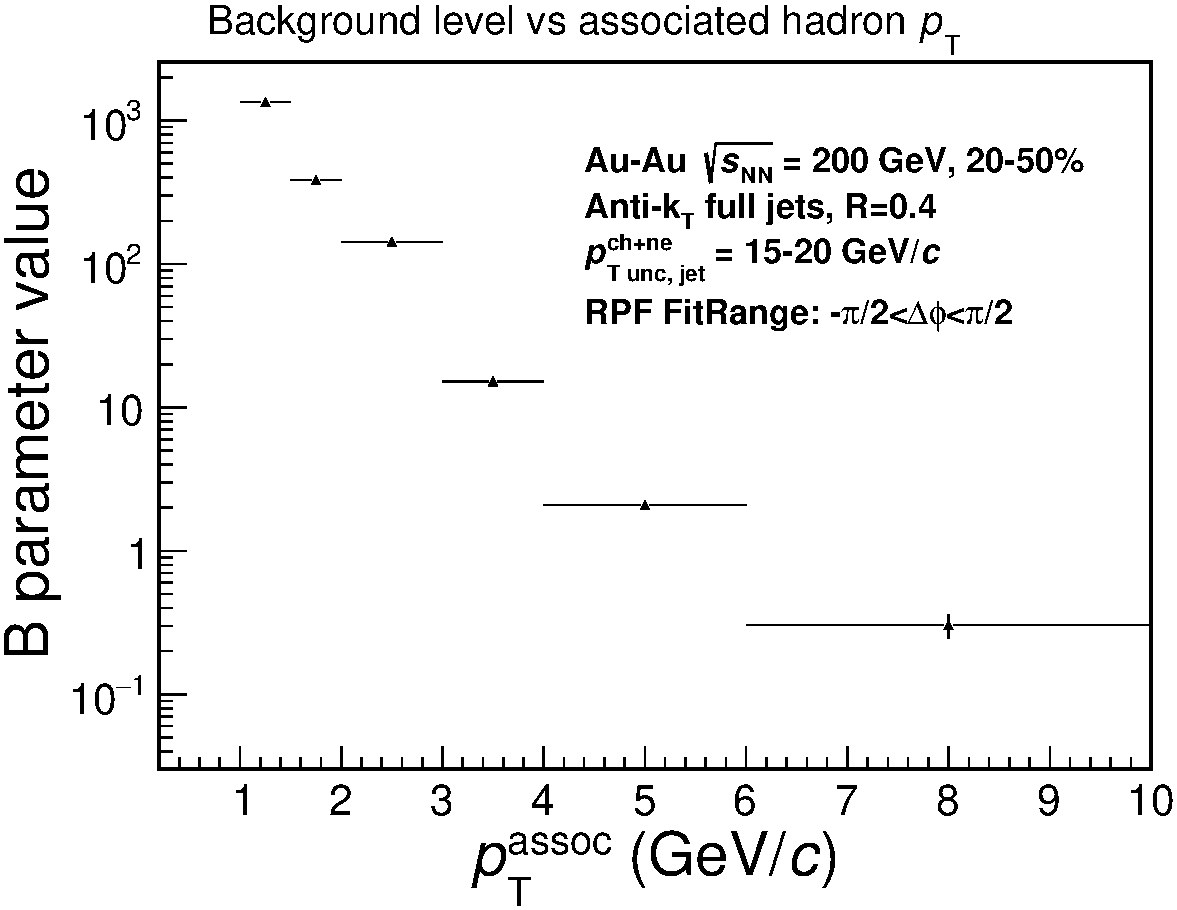
\includegraphics[width=\linewidth]{JHC/FitPars_Background_J15-20_C20-50_Zcut24.pdf}&
		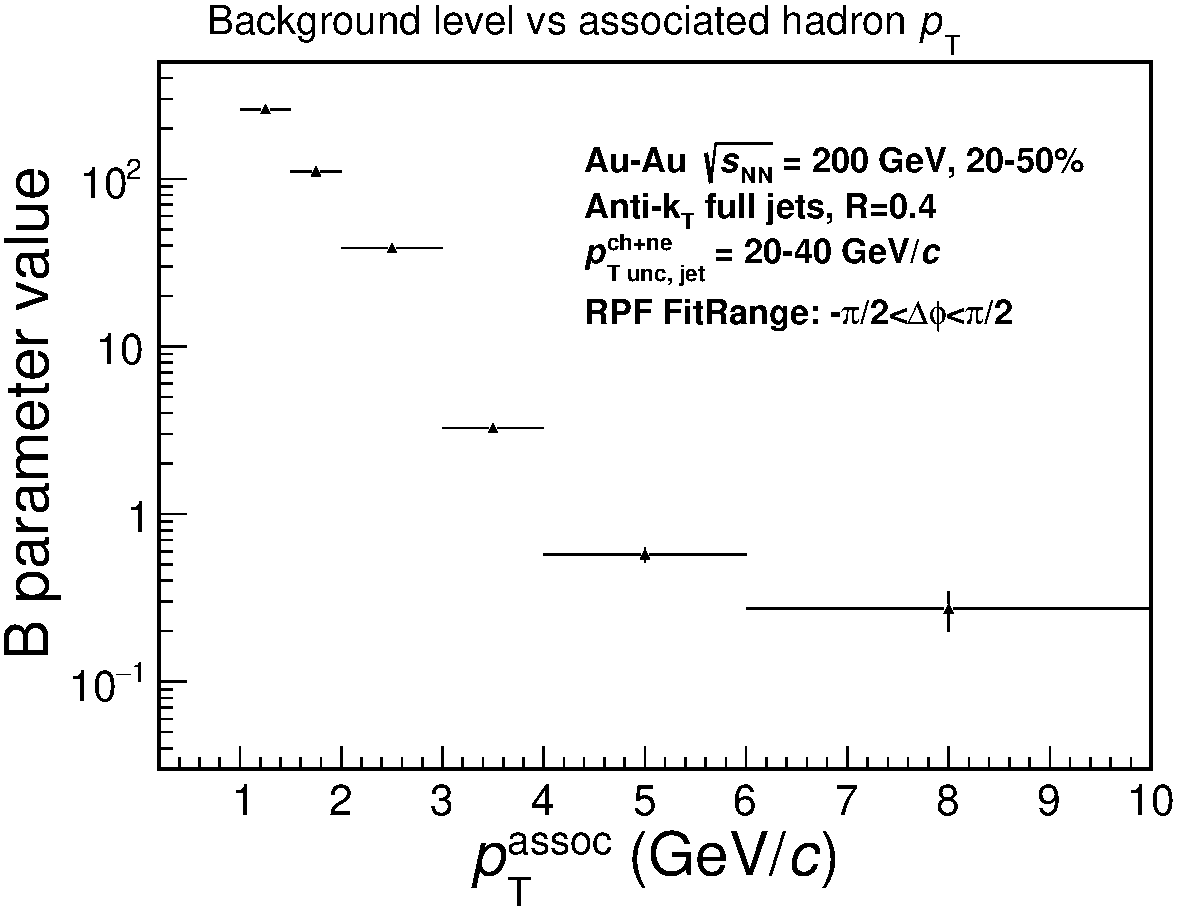
\includegraphics[width=\linewidth]{JHC/FitPars_Background_J20-40_C20-50_Zcut24.pdf}\\
		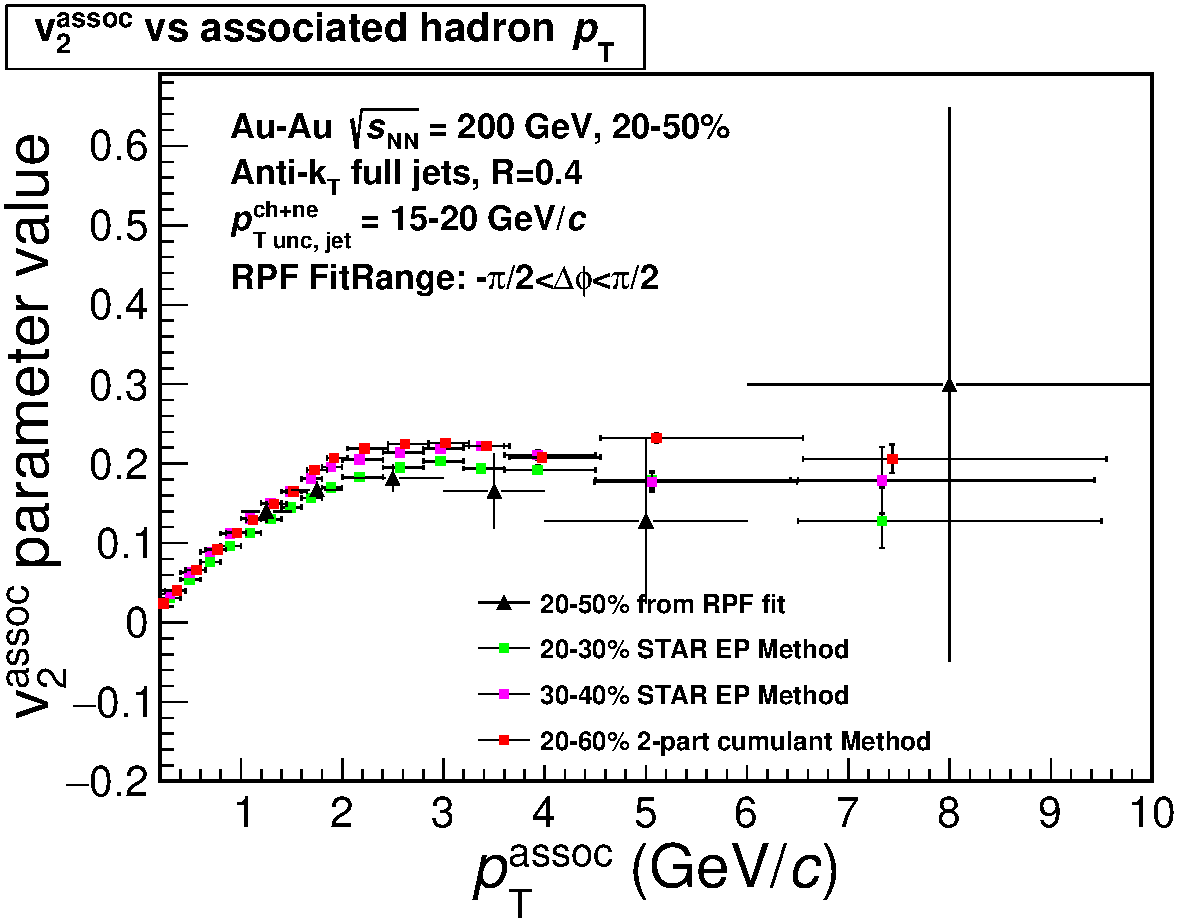
\includegraphics[width=\linewidth]{JHC/FitPars_v2Assoc_J15-20_C20-50_Zcut24.pdf}&
		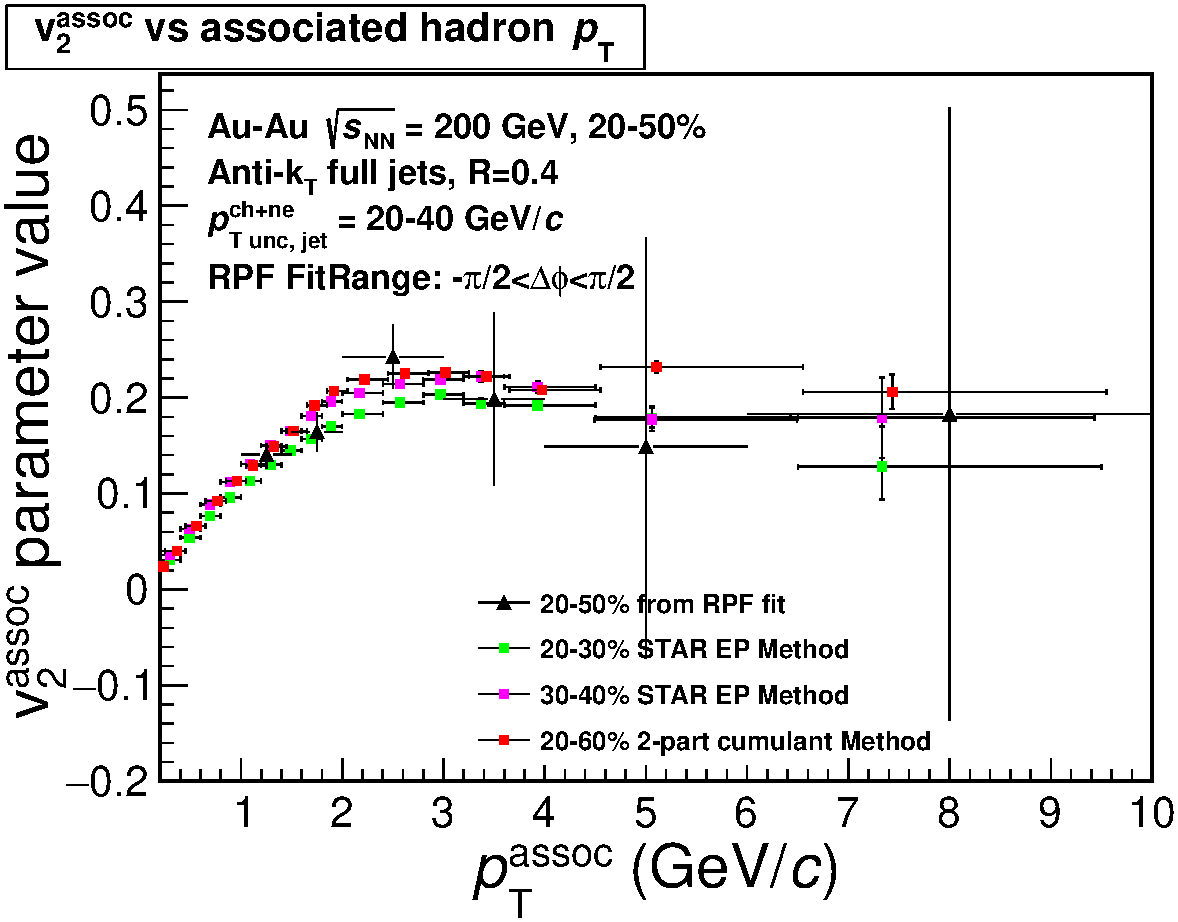
\includegraphics[width=\linewidth]{JHC/FitPars_v2Assoc_J20-40_C20-50_Zcut24.pdf}\\
%		\includegraphics[width=\linewidth]{JHC/FitPars_v2Jet_J15-20_C20-50_Zcut24.pdf}&
%	%	\includegraphics[width=\linewidth]{JHC/FitPars_v3sq_J15-20_C20-50_Zcut24.pdf}&
%		\includegraphics[width=\linewidth]{JHC/FitPars_v4Assoc_J15-20_C20-50_Zcut24.pdf}&
%		\includegraphics[width=\linewidth]{JHC/FitPars_v4Jet_J15-20_C20-50_Zcut24.pdf}&\\
%%
%		\includegraphics[width=\linewidth]{JHC/FitPars_v2Jet_J20-40_C20-50_Zcut24.pdf}&
%		\includegraphics[width=\linewidth]{JHC/FitPars_v3sq_J20-40_C20-50_Zcut24.pdf}&
%		\includegraphics[width=\linewidth]{JHC/FitPars_v4Assoc_J20-40_C20-50_Zcut24.pdf}&
%		\includegraphics[width=\linewidth]{JHC/FitPars_v4Jet_J20-40_C20-50_Zcut24.pdf}
	\end{tabularx}
	\caption[Parameters of the RPF fits as a function of \(p_\mathrm{T, assoc}\)]{Parameters of the RPF fits as a function of \Pt{assoc} for \pttrigrange{15}{20} (left) and \pttrigrange{20}{40} (right) full jets in 20--50\% central \AuAu collisions: the background level $B$ (top) and the second-order flow coefficient of the associated hadrons, $v_{2,\mathrm{assoc}}$ (bottom). The fits are performed over $|\dphi| < \pi/2$ in the background-dominated region $0.6 < |\deta| < 1.2$.}
	\label{fig:RPFpars}
\end{figure}

\begin{sidewaysfigure}
	\centering
		% OLD \includegraphics[width=16cm]{figures/plots/physics/PWfitBgExtract_A1.0-1.5_Trig15-20_C20-50_Zcut24.pdf}
	\begin{tabularx}{\textwidth}{XX}
		(a) & (b) \\
		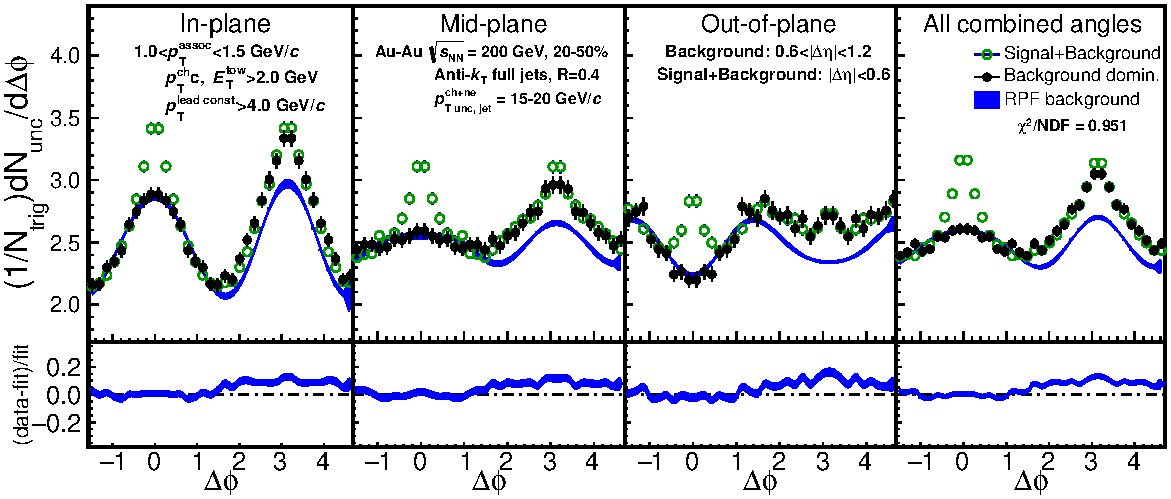
\includegraphics[width=\linewidth]{JHC/JHCorrBGsub_A1.0-1.5_T15-20_C20-50.pdf} &
		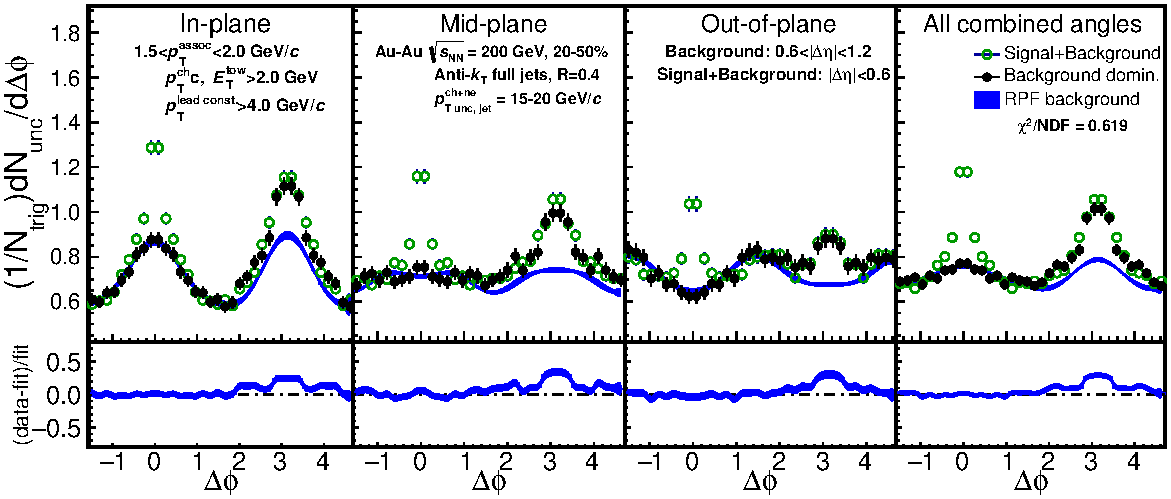
\includegraphics[width=\linewidth]{JHC/JHCorrBGsub_A1.5-2.0_T15-20_C20-50.pdf} \\
		(c) & (d) \\
		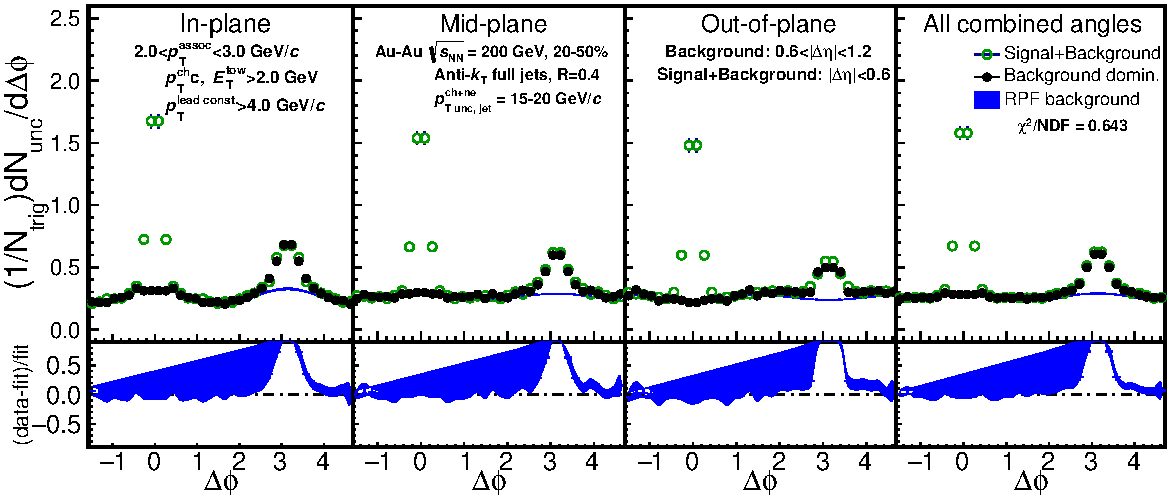
\includegraphics[width=\linewidth]{JHC/JHCorrBGsub_A2.0-3.0_T15-20_C20-50.pdf} &
		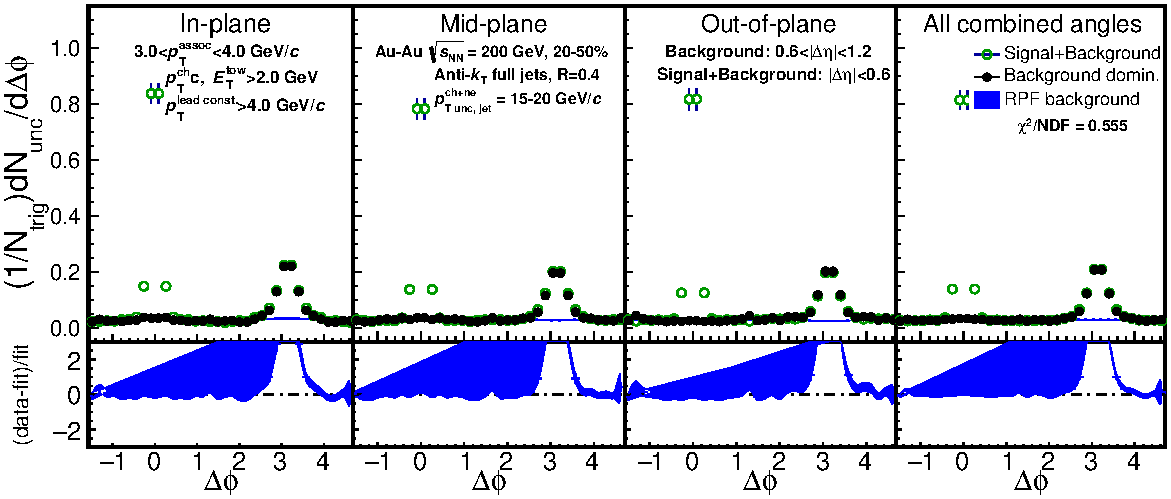
\includegraphics[width=\linewidth]{JHC/JHCorrBGsub_A3.0-4.0_T15-20_C20-50.pdf} \\
		(e) & (f) \\
		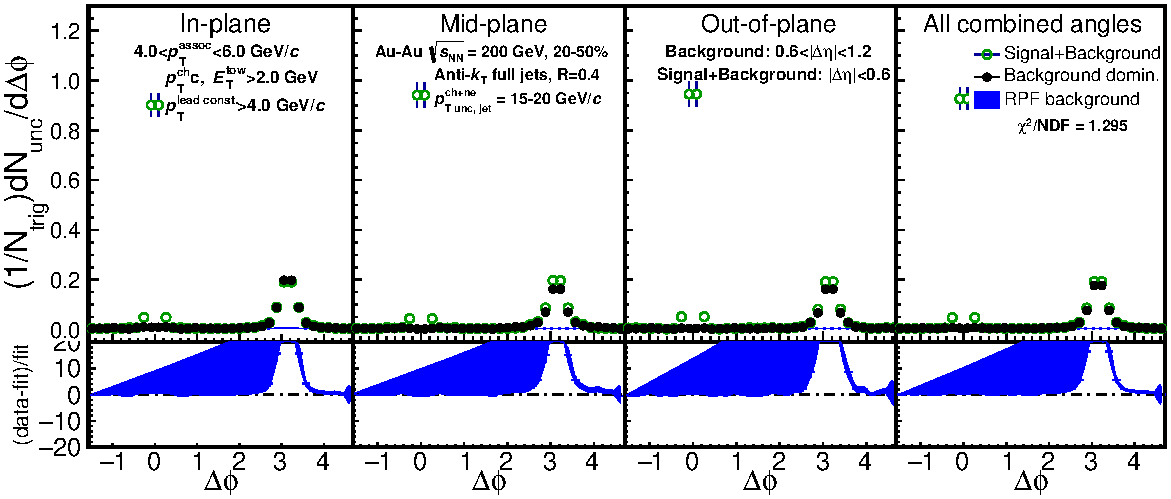
\includegraphics[width=\linewidth]{JHC/JHCorrBGsub_A4.0-6.0_T15-20_C20-50.pdf} &
		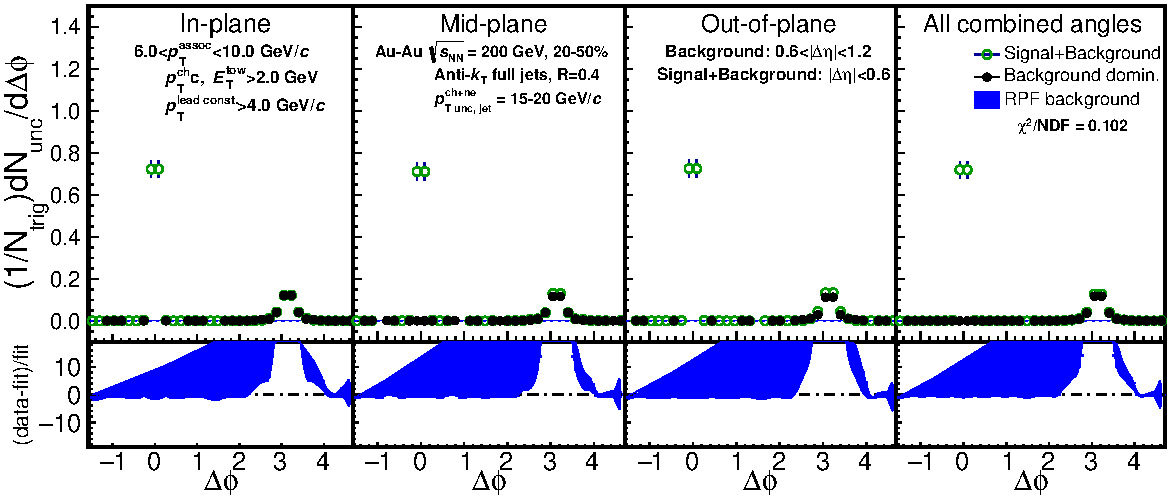
\includegraphics[width=\linewidth]{JHC/JHCorrBGsub_A6.0-10.0_T15-20_C20-50.pdf} \\
	\end{tabularx}
		\caption[RPF background fits for 15--20~GeV/\(c\) jets]{RPF fits for \pttrigrange{15}{20} full jets in 20--50\% central \AuAu collisions, for (a) \ptassocrange{1.0}{1.5}, (b) \ptassocrange{1.5}{2.0}, (c) \ptassocrange{2.0}{3.0}, (d) \ptassocrange{3.0}{4.0}, (e) \ptassocrange{4.0}{6.0} and (f) \ptassocrange{6.0}{10.0}. Each panel shows, from left to right, in-plane, mid-plane and out-of-plane jets and all orientations combined. Upper panels: \dphi projections of the signal+background region ($|\deta| < 0.6$, green) and of the background-dominated region ($0.6 < |\deta| < 1.2$, black), with the RPF fit to the background-dominated region (blue band, fit uncertainty). Lower panels: quality of the fit to the background-dominated region, (data $-$ fit)/fit.}
		\label{fig:RPFfitJ1520}
\end{sidewaysfigure}

\begin{sidewaysfigure}
	\centering
%		\rotatebox{0}{\resizebox{\textwidth}{!}{
%				%         \includegraphics{figures/SampleCorrelation.pdf}
%				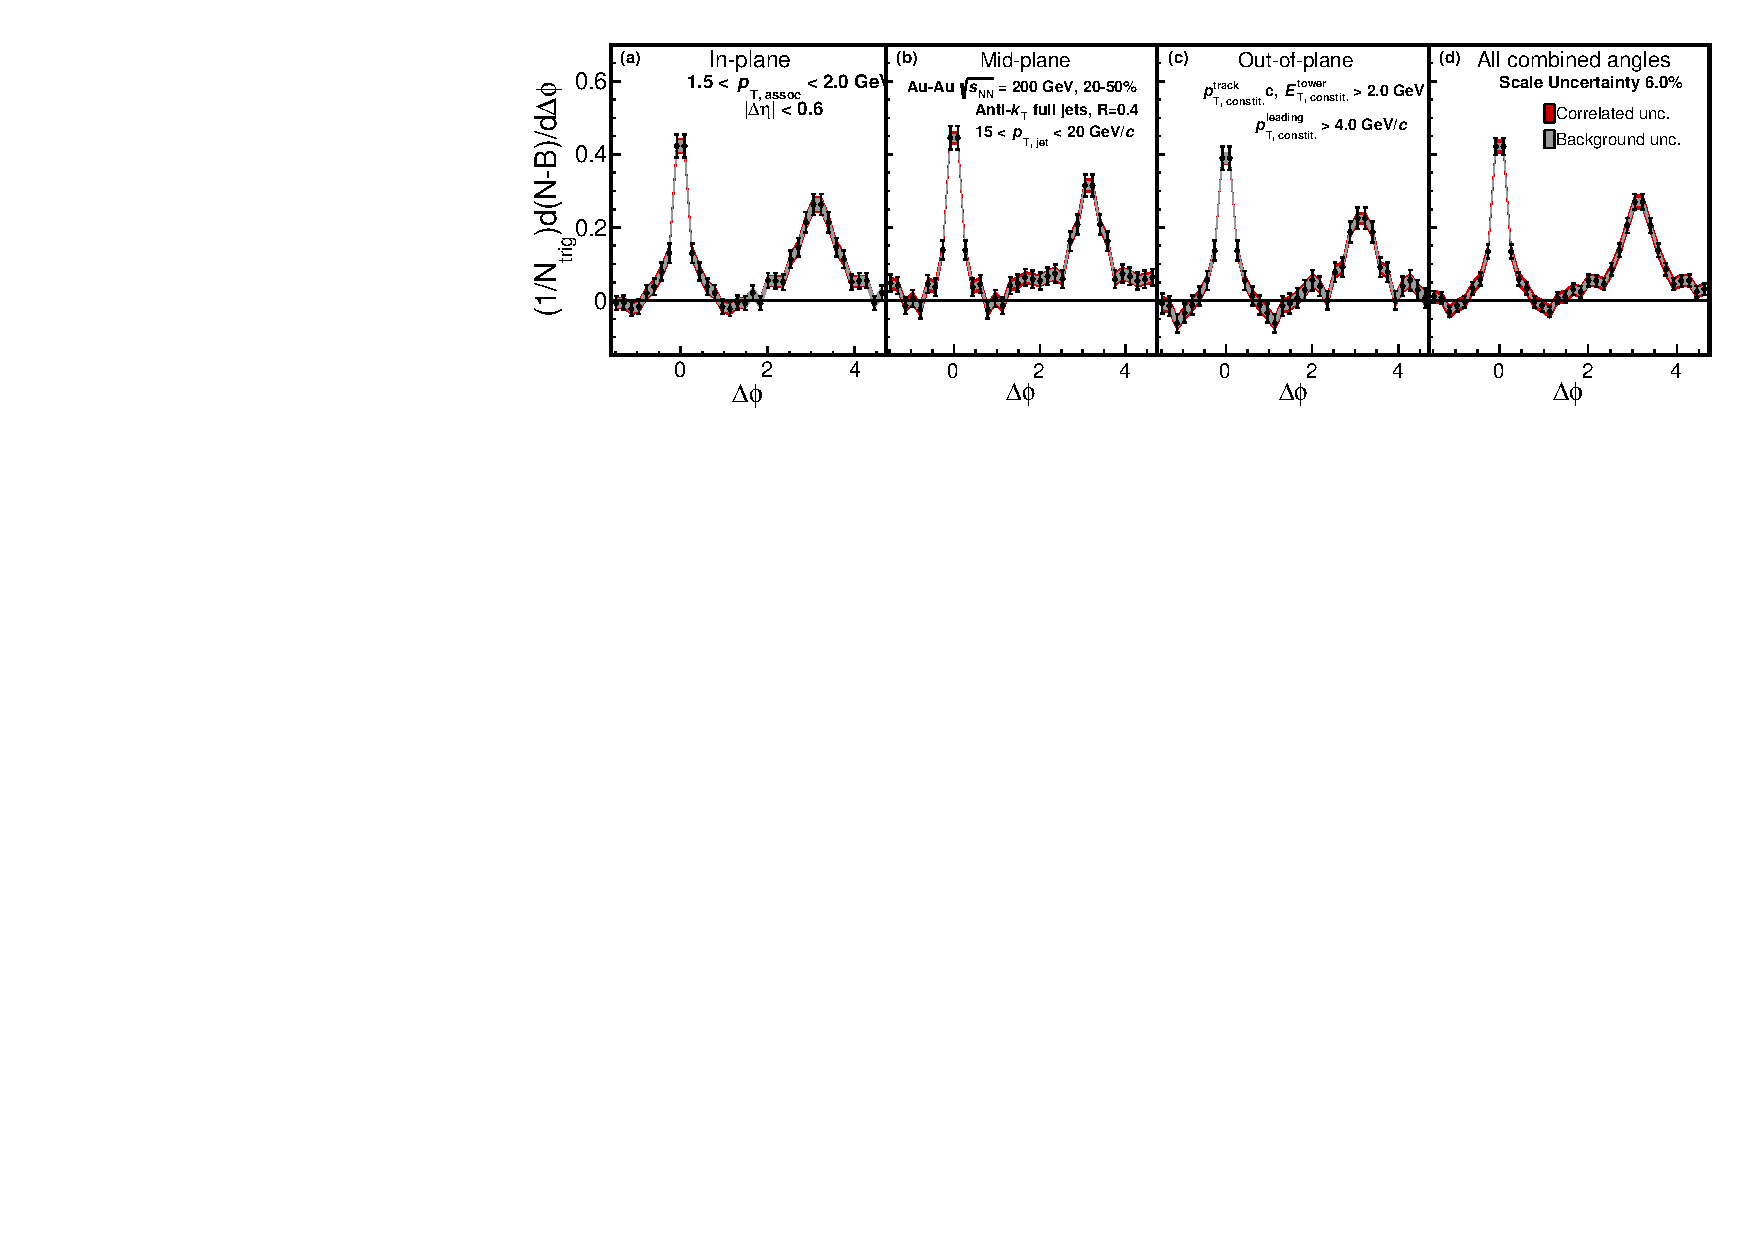
\includegraphics{figures/dPhiCorrelationsJ15-20_C20-50_1.5-2.0-paperplot.pdf}
%		}}
	\begin{tabularx}{\textwidth}{XX}
		(a) & (b) \\
	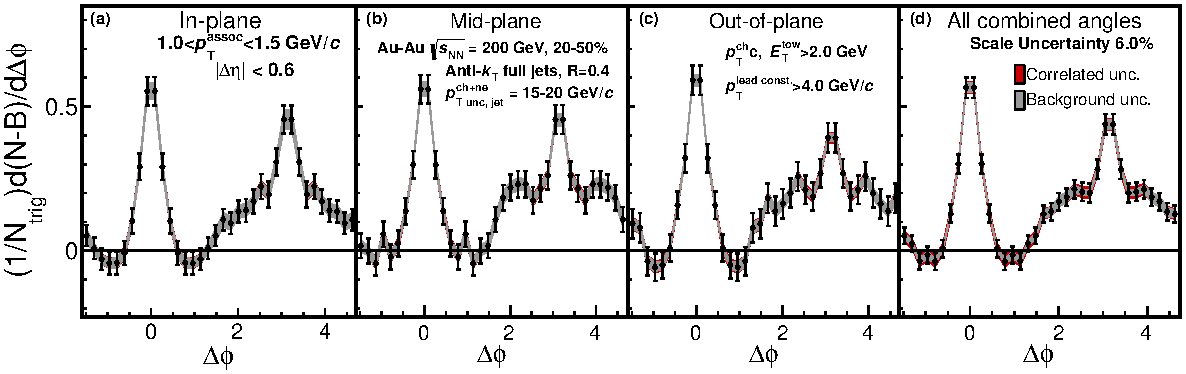
\includegraphics[width=\linewidth]{JHC/dPhiCorrelationsJ15-20_C20-50_1.0-1.5.pdf} &
	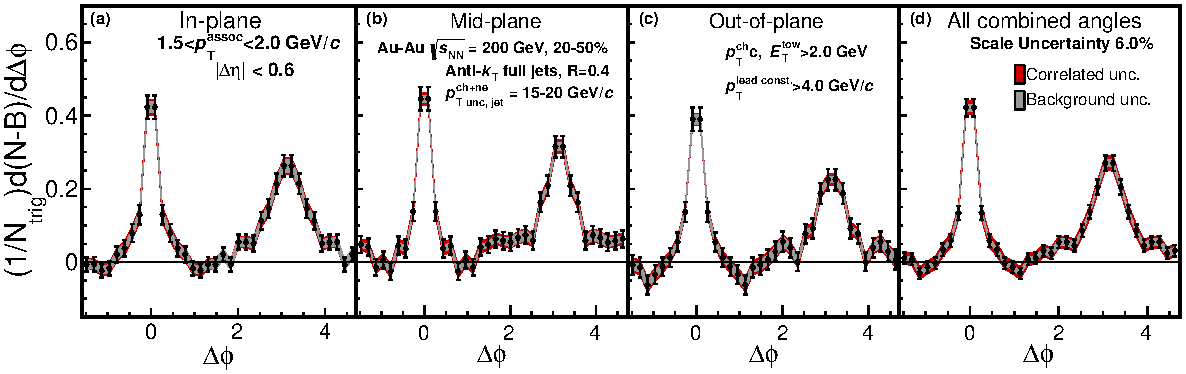
\includegraphics[width=\linewidth]{JHC/dPhiCorrelationsJ15-20_C20-50_1.5-2.0.pdf} \\
			(c) & (d) \\
	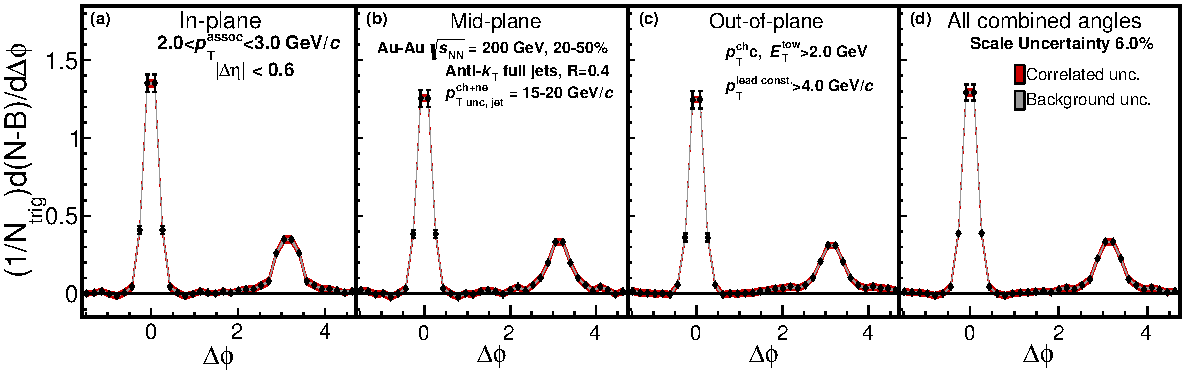
\includegraphics[width=\linewidth]{JHC/dPhiCorrelationsJ15-20_C20-50_2.0-3.0.pdf} &
	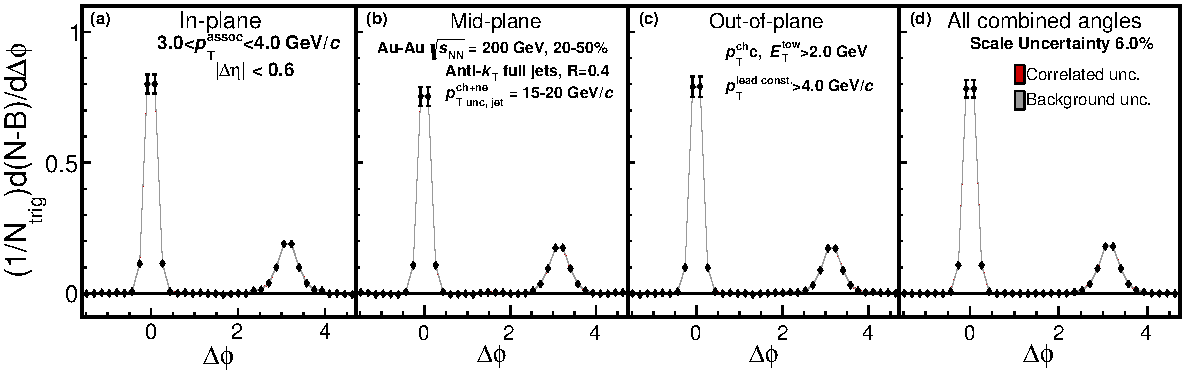
\includegraphics[width=\linewidth]{JHC/dPhiCorrelationsJ15-20_C20-50_3.0-4.0.pdf} \\
			(e) & (f) \\
	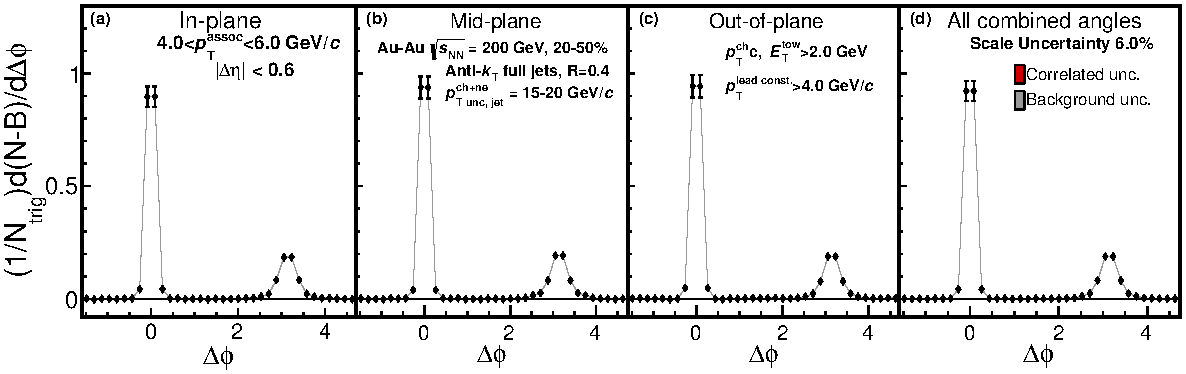
\includegraphics[width=\linewidth]{JHC/dPhiCorrelationsJ15-20_C20-50_4.0-6.0.pdf} &
	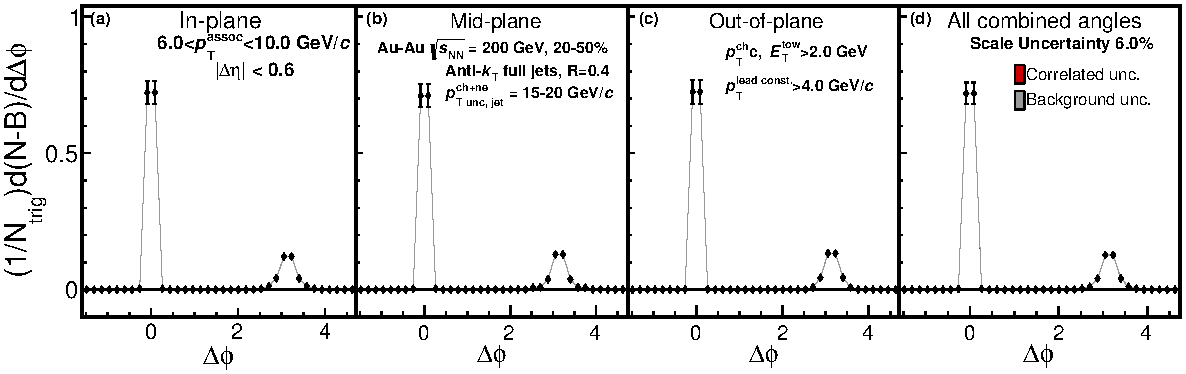
\includegraphics[width=\linewidth]{JHC/dPhiCorrelationsJ15-20_C20-50_6.0-10.0.pdf} \\
\end{tabularx}

		\caption[Background-subtracted jet-hadron correlations for 15--20~GeV/\(c\) jets]{Background-subtracted jet-hadron correlation functions in \dphi ($|\deta| < 0.6$) for \pttrigrange{15}{20} full jets in 20--50\% central \AuAu collisions, for (a) \ptassocrange{1.0}{1.5}, (b) \ptassocrange{1.5}{2.0}, (c) \ptassocrange{2.0}{3.0}, (d) \ptassocrange{3.0}{4.0}, (e) \ptassocrange{4.0}{6.0} and (f) \ptassocrange{6.0}{10.0}. Each panel shows in-plane, mid-plane and out-of-plane jets and all orientations combined. The red band is the correlated scale uncertainty from the mixed-event acceptance correction and the gray band is the uncertainty of the RPF background fit, which is correlated point-to-point; the global scale uncertainty of 6\% is not shown.}
		\label{fig:dPhiJ1520}
\end{sidewaysfigure}

\begin{sidewaysfigure}
	\centering
	\begin{tabularx}{\textwidth}{XX}
		(a) & (b) \\
	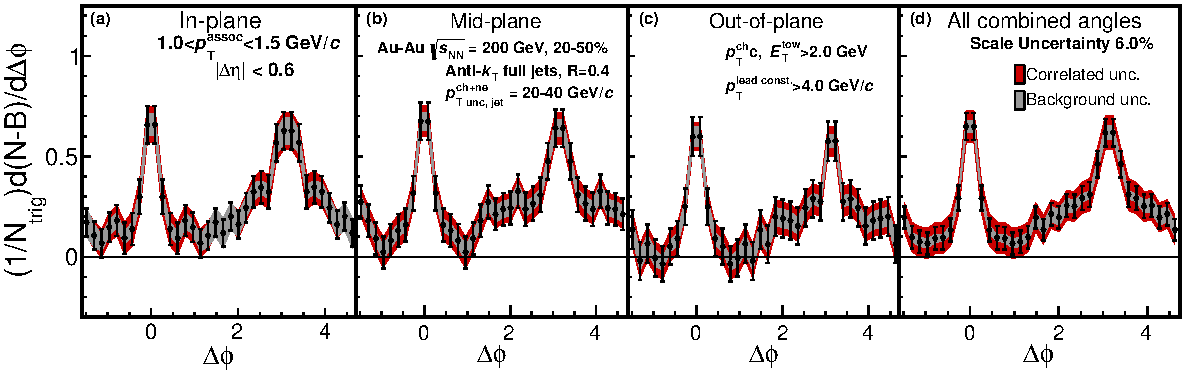
\includegraphics[width=\linewidth]{JHC/dPhiCorrelationsJ20-40_C20-50_1.0-1.5.pdf} &
	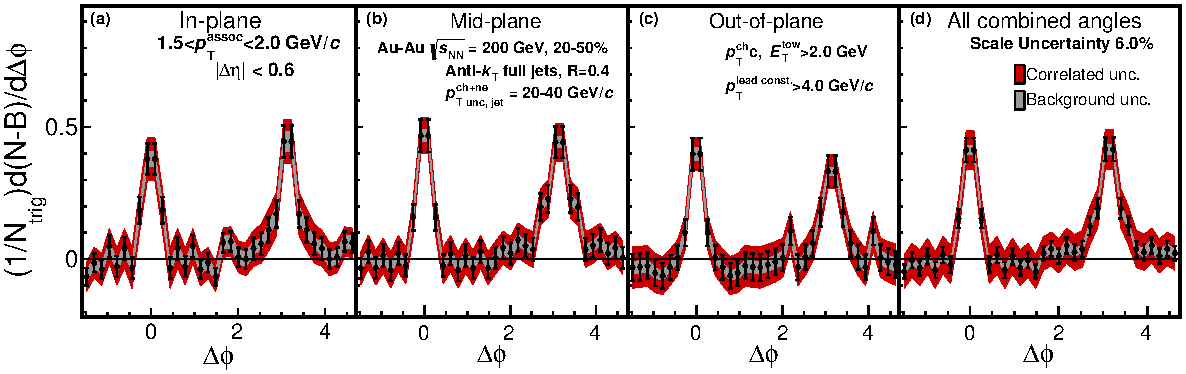
\includegraphics[width=\linewidth]{JHC/dPhiCorrelationsJ20-40_C20-50_1.5-2.0.pdf} \\
			(c) & (d) \\
	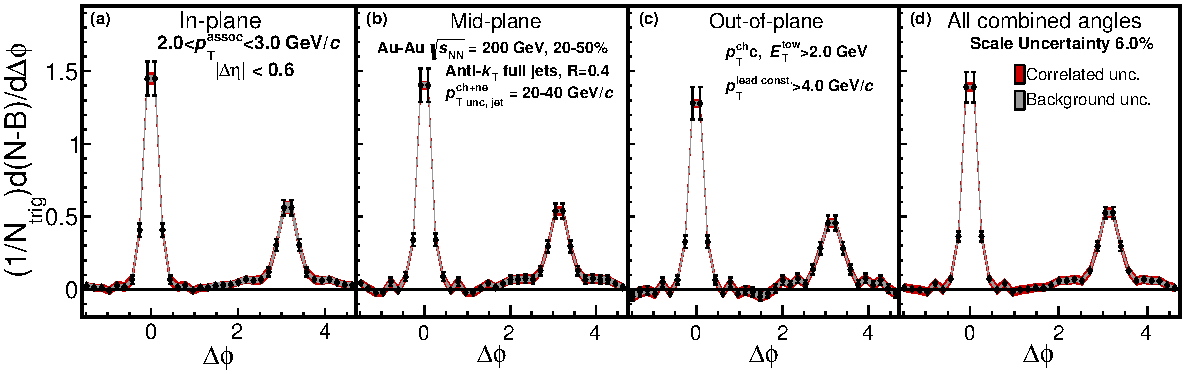
\includegraphics[width=\linewidth]{JHC/dPhiCorrelationsJ20-40_C20-50_2.0-3.0.pdf} &
	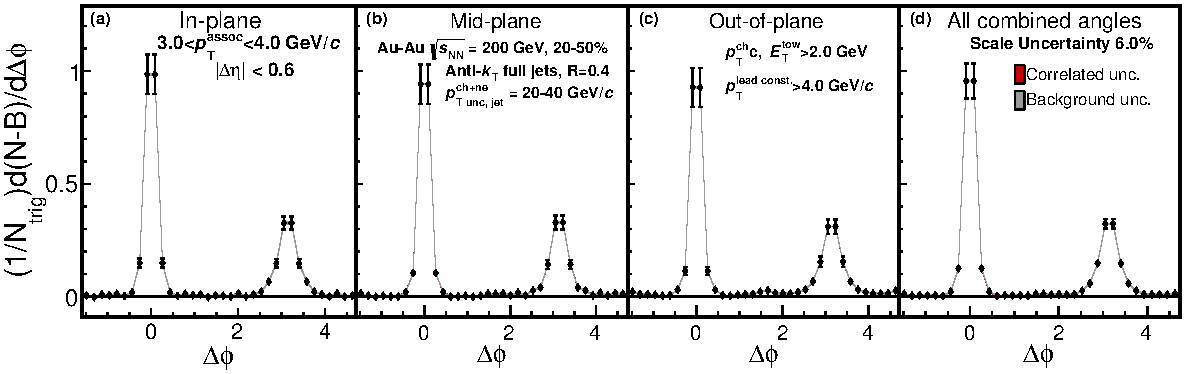
\includegraphics[width=\linewidth]{JHC/dPhiCorrelationsJ20-40_C20-50_3.0-4.0.pdf} \\
			(e) & (f) \\
	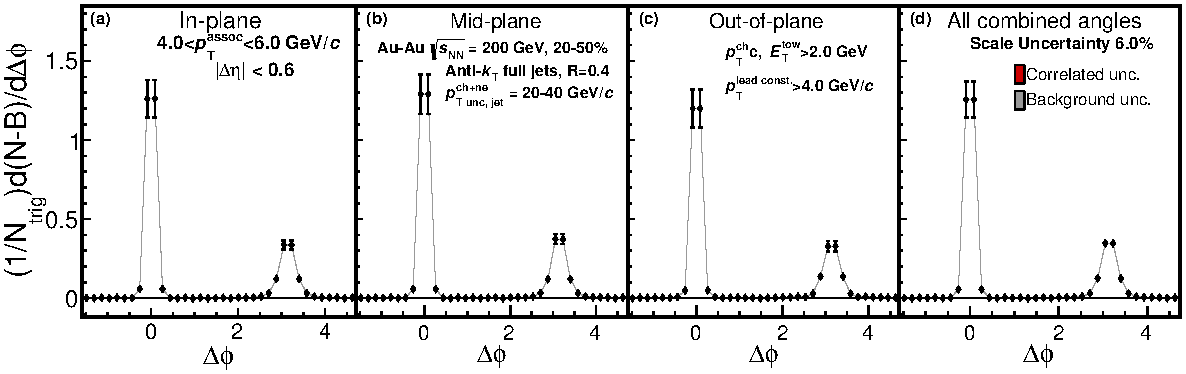
\includegraphics[width=\linewidth]{JHC/dPhiCorrelationsJ20-40_C20-50_4.0-6.0.pdf} &
	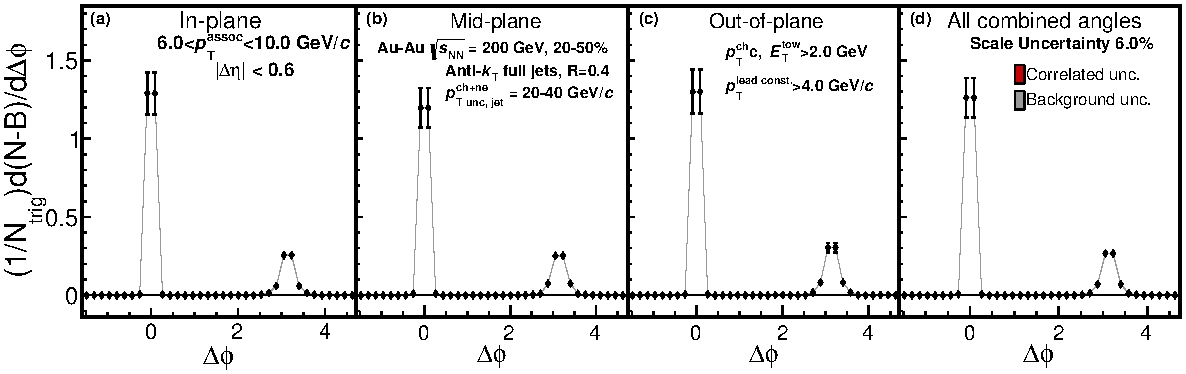
\includegraphics[width=\linewidth]{JHC/dPhiCorrelationsJ20-40_C20-50_6.0-10.0.pdf} \\
\end{tabularx}

		\caption[Background-subtracted jet-hadron correlations for 20--40~GeV/\(c\) jets]{Same as Fig.~\ref{fig:dPhiJ1520}, for \pttrigrange{20}{40} full jets.}
		\label{fig:dPhiJ2040}
\end{sidewaysfigure}

Comparison of in-, mid-, and out-of-plane jet-hadron correlations is performed after background subtraction to explore the effects related to event-plane orientation.
%
The background-subtracted correlation functions are shown in Figs.~\ref{fig:dPhiJ1520} and~\ref{fig:dPhiJ2040} for \pttrigrange{15}{20} and \pttrigrange{20}{40} jets, respectively.
%
Each panel corresponds to one \Pt{assoc} bin and shows the in-plane, mid-plane, and out-of-plane jets and all orientations combined.
%
The uncertainties from the RPF background subtraction are propagated using Eq.~\ref{eqn:CovProp} and are non-trivially correlated point-to-point and between different bins relative to the event plane.  These are shown in gray.  The uncertainty from the acceptance correction, described in Sec.~\ref{sect:MixedEvents} is displayed by the red uncertainty band. The uncertainties on the event-plane resolution are negligible relative to that of the background subtraction and statistical uncertainties of the final results.  Additional uncertainties uncorrelated with each other, but correlated for all points in \dphi are given in Tab.~\ref{Tab:SystematicSummary}.  They are combined in quadrature and listed as the scale uncertainty on the results.

\subsection{Detector response and embedding closure} \label{sec:AuAuEmbedding}
The PYTHIA\mbox{-}6 Perugia 2012 tune is used to create particle-level dijet events embedded in MB \AuAu 200 GeV events at the detector level.
%
The events are generated in bins of the partonic hard-scattering transverse momentum, $\hat{p}_\mathrm{T}$, and the bins are combined with weights given by their cross sections divided by the number of generated events.  This allows for further comparisons between the jets from the input PYTHIA\mbox{-}6 tracks (generator-level jets or GEN-jets) and the jets from the embedded tracks reconstructed by GEANT (reconstructed jets or RECO-jets). RECO-level events are analyzed with the same selections and parameters as used by the data analysis. The GEN-level events consist of the final-state particles of the generator record, i.e.\ the particles the generator does not decay further. Long-lived particles that decay weakly, such as \(K^0_\mathrm{S}\) and \(\Lambda\), are kept stable by the generator and therefore appear at the GEN level as single particles; they are decayed by GEANT in the detector simulation, so that their decay products appear only in the RECO-level events. GEN-level jets have $\ptGenJet > $ 10 \GeVc and the RECO-level jets have $\ptRecoJet >$ 5 \GeVc. Further, only the RECO-level jets are required to contain a neutral component with $ E_{\rm T} \geq 5.4$ GeV to match the trigger condition applied in data. The goal is to study the effects of the detector response on jet reconstruction and on the analysis.  In order to compare the same jet pre- and post-reconstruction, a `nearness' criterion is applied in the $\eta-\phi$ plane that matches a GEN-jet to one RECO-jet satisfying: 

(a) $r_{\rm GEN, RECO}=\sqrt{(\eta^{\rm GEN}_{\rm jet}-\eta^{\rm RECO}_{\rm jet})^2+(\phi^{\rm GEN}_{\rm jet}-\phi^{\rm RECO}_{\rm jet})^2}\leq0.4$, $r_{\rm GEN, RECO}$ being the separation between the gen-jet and the reco-jet in $\eta-\phi$ space, (b) the RECO-jet is the closest to the gen-jet among all reco-jets (minimize $r_{\rm GEN, RECO}$).  

The resulting GEN- and RECO-level jet spectra are compared to calculate the momentum resolution which is given by:

\begin{equation}
	\Pt{jet} \textnormal{ resolution} (\%) = \frac{\text{\ptGenJet} - \text{\ptRecoJet}}{\text{\ptGenJet}} \times \text{100} \%.
	\label{Eq:JetPtRes}
\end{equation}

% The jets are constructed with the same parameters as the main analysis at both the gen- and reco-levels.  For comparing the jets before and after they go through the detectors, we need to be somewhat sure that we are comparing the same jet pre- and post-reconstruction.  But unfortunately, we don't have the information about which gen-jet exactly went through the detector to give us a particular reco-jet.  Thus we need some kind of a matching criteria to match a gen-jet to a reco-jet.  In this study, we have used a `nearness'  criteria in the $\eta$-$\phi$ space.  In a particular event, for each gen-jet, we keep the one reco-jet that is:

% \begin{enumerate}
	% 	\item Has less than $r=0.4$ separation from the gen-jet in the $\eta$-$\phi$ space. 
	% 	\item Is the closest to the gen-jet among the reco-jets. 
	% \end{enumerate}

%   Upon meeting the above two conditions, the reco-jet is matched to the gen-jet. 

%   \subsection{Response Matrices}
%%%%%%%%%%% Each such distribution is normalized within the region $20 \leq \ensuremath{p_{\rm T}}\xspace < 100$ \GeVc where fluctuations are minimized and, assuming that the jet energy distribution in the data is the same as that provided by PYTHIA\mbox{-}6, describes the generator level jet distribution that corresponds to the measured detector level jet distribution, shown in Fig.~\ref{plot:exampleParticleJetDistribution}. 

Fig.~\ref{fig:jetptresWinset} shows the \Pt{jet} resolution for $15 < \ptGenJet < 20$ \GeVc (left) and $20 < \ptGenJet < 40$ \GeVc (right) $R=0.4$ full jets.  The distributions have been normalized into probability functions and are shown for the 20--50\% most central events for all angles of the jet relative to the event plane.  Fig.~\ref{fig:jetptresWinset} further shows an average energy loss of around 15\% going from GEN to RECO. This net energy shift is thought to be due to two counteracting effects: the tracking inefficiency, which removes particles from the RECO-jets, and the underlying event of the MB \AuAu events into which the PYTHIA\mbox{-}6 events are embedded, whose particles are clustered into the RECO-jets as well and add to their momentum. The \Pt{jet} resolution for $15 < \ptRecoJet < 40$ \GeVc reco-jets is roughly 10--20\%.  The event-plane dependence of the \Pt{jet} resolution was also studied, and the resolutions for the different jet orientations relative to the event plane agree within 1--2\%.  There can be slight differences in the jets reconstructed at lower momenta with \pttrigrange{15}{20} for jets at different angles relative to the event plane, due to a low momentum embedded jet overlapping with another jet in the \AuAu data and from statistical fluctuations.  As there are more jets from in-plane than out-of-plane orientations in the data, this leads to an apparent difference in the reconstructed jet spectra. Otherwise there are no significant differences between jets at different angles relative to the event plane. A map between \ptGenJet and  \ptRecoJet, called the response matrix, is added to Fig.~\ref{fig:jetptresWinset} as a smaller inset on the top right.
%
Since the trigger jets are selected at the detector level and the results are not unfolded, these numbers characterize which particle-level jets populate the two reconstructed jet-momentum classes rather than enter as a correction.

%The uncertainty on the jet energy scale is \commented[ADD \%] and the jet energy resolution, which is also encoded in the response matrix, is around \commented[ADD \%] for the jets selected in this analysis.  Further results from the embedding for gen-level and reco-level jets can be found in Sec.~\ref{sect:Results}.

\begin{figure}[!htbp]
	\centering
	% OLD	\includegraphics[width=0.99\linewidth]{figures/plots/Embedding/EmbPlot_vers4.pdf}
	%	\includegraphics[width=0.99\linewidth]{figures/plots/Embedding/EmbPlot-momentum-resolution.pdf}
	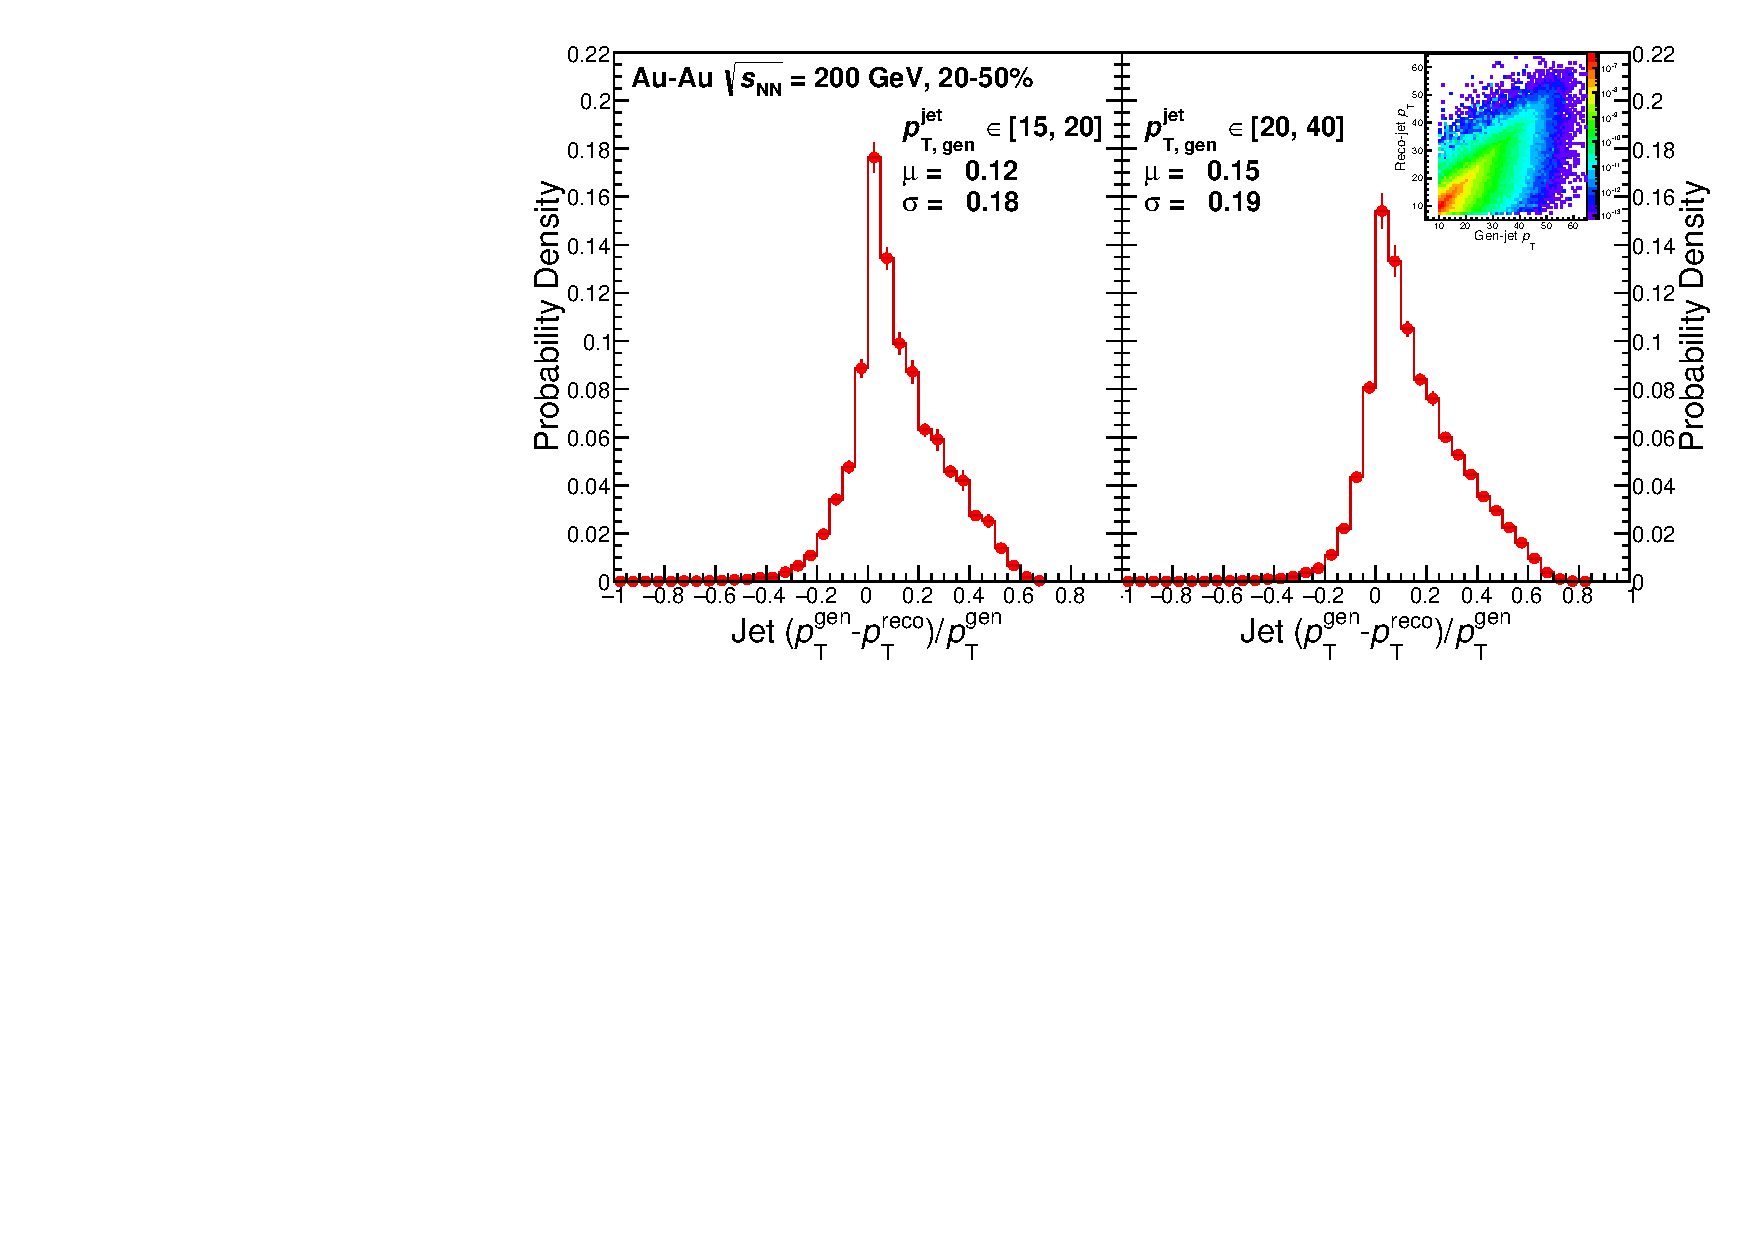
\includegraphics[width=0.99\linewidth]{figures/EmbPlot_pt_resolution_w_inset.pdf}
	\caption[Jet-\(p_\mathrm{T}\) resolution and response matrix of the Au+Au embedding]{\Pt{jet} resolution for $15 < \ptGenJet < 20$ \GeVc (left) and $20 < \ptGenJet < 40$ \GeVc (right) $R=0.4$ full jets with the corresponding response matrix as an inset on the top right.  Jets are measured from all angles relative to the event plane in the 20--50\% most central events.  This comparison is for matched GEN-level to RECO-level jets. }
	\label{fig:jetptresWinset}
\end{figure}

The same embedding sample is used for a closure test of the analysis chain.
%
The associated yields and jet-peak widths are extracted from the RECO-level jets with the full analysis procedure, including the mixed-event correction taken from data and the RPF background subtraction, and compared to those of the matched GEN-level jets, whose correlations with the final-state PYTHIA\mbox{-}6 particles contain no combinatorial background.
%
The comparison is complicated by the tracking efficiency near a jet, which differs from the average efficiency used in the correction: above 2~\GeVc it is slightly lower inside \pttrigrange{15}{20} jets and slightly higher inside \pttrigrange{20}{40} jets than for an average track in the event.
%
After correcting the RECO-level near-side yields for this difference, the RECO/GEN ratio of the yields for \pttrigrange{20}{40} jets, shown in Fig.~\ref{fig:ClosureJ2040}, is consistent with unity on the away side.
%
The remaining deviations, on the near side in the highest \Pt{assoc} bin and in the lowest \Pt{assoc} bins for \pttrigrange{15}{20} jets, were traced to the limited statistics of the low-$\hat{p}_\mathrm{T}$ bins of the embedding, which enter with large weights.

\begin{figure}[!htbp]
	\centering
	% white box covers the stale "points displaced for visibility" label (single series only)
	\begin{tikzpicture}
		\node[anchor=south west, inner sep=0] (img) {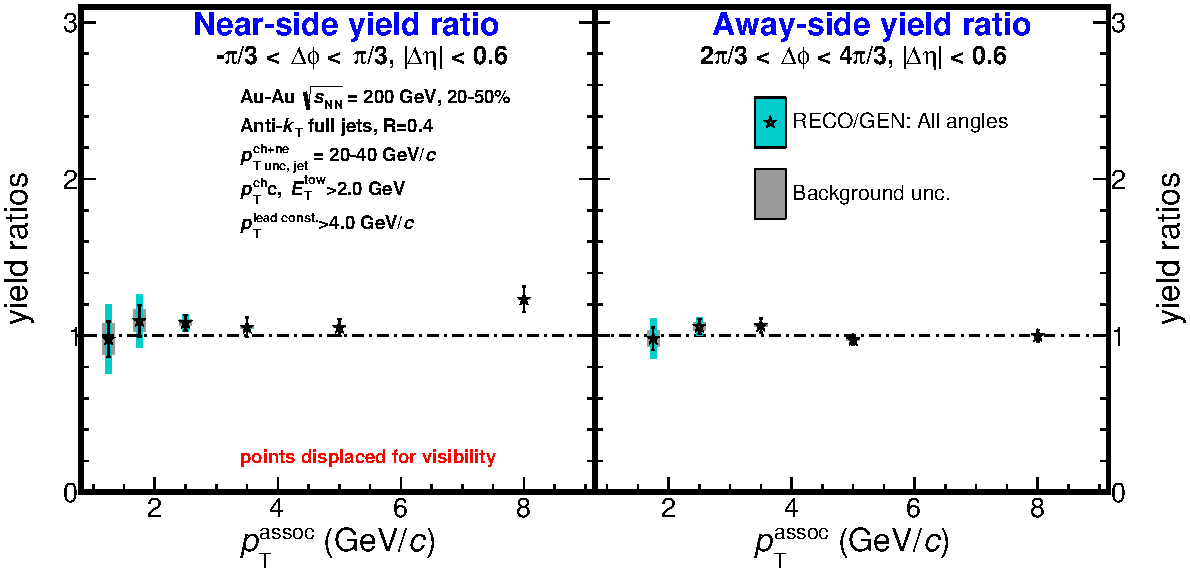
\includegraphics[width=0.99\linewidth]{JHC/NearAwaySideYieldRatioRECO-GEN_J20-40_C20-50_onlyALL_withEffCorr.pdf}};
		\begin{scope}[x={(img.south east)}, y={(img.north west)}]
			\fill[white] (0.198,0.182) rectangle (0.420,0.228);
		\end{scope}
	\end{tikzpicture}
	\caption[Embedding closure test of the associated yields for 20--40~GeV/\(c\) jets]{Embedding closure test: ratio of the near-side (left) and away-side (right) associated yields extracted from RECO-level jets to those of the matched GEN-level jets vs \Pt{assoc}, for \pttrigrange{20}{40} full jets embedded in 20--50\% central \AuAu events, all orientations relative to the event plane combined. The RECO-level near-side yields are corrected for the tracking efficiency inside jets (see text). The gray bands are the uncertainties of the RPF background fit.}
	\label{fig:ClosureJ2040}
\end{figure}

\subsection{Systematic uncertainties} \label{sect:SysUnc}
The systematic uncertainties fall into three classes that differ in how they are correlated, and therefore in how they are shown on the results.
%
(i) Sources that change the overall normalization of the correlation functions, independently of \dphi and of the jet orientation, are combined into a global scale uncertainty: the single-track reconstruction efficiency, the normalization of the mixed events, and the event-plane resolution.
%
(ii) Sources that change the level of the correlation functions in a way that depends on \Pt{assoc} and on the jet orientation are shown as colored scale bands: the shape of the pair acceptance in \deta and the jet-energy-shift (JES) correction.
%
(iii) The uncertainty of the RPF background fit, obtained from the covariance matrix of the fit, varies from point to point in \dphi and is correlated between points and between orientations; it is shown as a gray band.
%
Each source is described below.

The 5\% uncertainty on the single-track reconstruction efficiency (Sec.~\ref{sec:TrackTowerSel}) directly scales the number of associated hadrons, and hence the yields, while leaving the shape of the correlation functions unchanged.
%
The mixed-event normalization uncertainty is the uncertainty of the constant fitted to the plateau of the pair acceptance (Sec.~\ref{sect:MixedEventsUnc}).
%
The event-plane resolution enters only through the background parametrization, since the signal itself is not corrected for the resolution (Sec.~\ref{sec:EPReco}); varying it by $\pm 1\%$ changes the results negligibly.

The systematic uncertainties are summarized in Tabs.~\ref{Tab:SystematicSummary}, \ref{Tab:SystematicSummaryEPdep}, and~\ref{Tab:SystematicSummaryEPdep2040}.  Tab.~\ref{Tab:SystematicSummary} lists the sources of systematic uncertainties which are independent of the angle relative to the event plane.  These sources include the single-track reconstruction efficiency (Sec.~\ref{sec:TrackTowerSel}), 
%contamination from secondaries (Sec.~\ref{sect:STARdet}), 
uncertainties in the mixed events due to their normalization and shape in \dphi (Sec.~\ref{sect:MixedEventsUnc}), and uncertainties in the event-plane resolution (Sec.~\ref{sect:Method}).  The uncertainties are added in quadrature and lead to a 6\% uncertainty in the scale of the correlation functions and yields with the single-track reconstruction efficiency being the dominant source.  This uncertainty is uncorrelated for different associated-particle momenta.

\begin{table}[!htbp]
	\caption[Systematic uncertainties independent of the jet orientation]{Summary of systematic uncertainties which are independent of the angle relative to the event plane and the momentum for both \pttrigrange{15}{20} and \pttrigrange{20}{40} in 20--50\% central \AuAu collisions.}
	\label{Tab:SystematicSummary}
	\centering % used for centering table
	\begin{tabular}{l | c} % centered columns
		\hline % inserts double horizontal lines
		Source & Uncertainty \% \Tstrut \Bstrut \\ % inserts table heading
		\hline % inserts single horizontal line
		Single particle reconstruction efficiency & 5 \\
		%\hline
		%Contamination & 1 \\
		\hline
		Mixed event (shape \dphi) & negligible \\
		\hline
		Mixed event normalization & $< 1.25$ \\ 
		\hline
		Event-plane resolution &  $< 1$ \\ 
		\hline
	\end{tabular}
\end{table}

Additional uncertainties, highly dependent on the angle of the jet relative to the event plane and the associated particles' momentum, are summarized in Tabs.~\ref{Tab:SystematicSummaryEPdep} and~\ref{Tab:SystematicSummaryEPdep2040}.  These include the impact of the scale uncertainty from the acceptance shape (Sec.~\ref{sect:MixedEvents}, Eq.~\ref{Eqtn:alpha}) and the RPF background fit (Sec.~\ref{sect:CorrBkgd}) on the associated yield and jet-peak width results.  These uncertainties are compared for two associated particle momentum bins (1.0--1.5 and 3.0--4.0~\GeVc) to highlight how much of an impact the background has at low momenta.  The uncertainty arising from the RPF background subtraction is non-trivially correlated point-to-point in \dphi and for different orientations of the jet relative to the event plane, but is uncorrelated between different \Pt{assoc} bins.  The acceptance-correction uncertainty on the shape in \deta is also correlated for different orientations of the jet relative to the event plane and uncorrelated across \Pt{assoc} bins.  The acceptance-shape uncertainty is the dominant source at low momenta, while being more comparable to the background uncertainty at larger momenta.  

Since no underlying-event subtraction is applied to the jets (Sec.~\ref{sec:JetRecoAuAu}), background particles that fall into the jet cone shift the reconstructed jet momentum upward, and the shift is larger for in-plane than for out-of-plane jets because the flow-modulated background is larger in-plane.
%
Jets in the different orientations therefore sample slightly different parton momenta for the same reconstructed \Pt{jet} class.
%
To account for this jet-energy shift (JES) and to provide an adequate comparison for the jet samples from different orientations relative to the event plane, a random-cone study was performed on the minimum-bias data of matching centrality selection: cones of radius 0.4 are placed at random positions within the jet acceptance, and the transverse momenta of the charged particles inside them are summed, in bins of the cone orientation relative to the event plane.
%
The mean summed momenta are found to be 0.388 \GeVc (in-plane), 0.344 \GeVc (mid-plane), and 0.308 \GeVc (out-of-plane), with a corresponding RMS of 0.4 \GeVc.
%
To determine the effect on the results, the correlation functions are also constructed for jet-momentum classes shifted by a fixed amount, and the resulting changes of the yields and widths are rescaled to the shifts found with the random cones.
%
The nominal yields and widths are corrected by these rescaled shifts, and the corresponding rescaled RMS is assigned as the JES uncertainty, which is added in quadrature to the acceptance-shape scale uncertainty.

% jet energy scale correction

%Both of these sources are stronger on the near-side at low-momenta, while being stronger on the away-side for higher momenta.

% ------------------------ 15-20 GeV ---------------------------------
\begin{table}[!htbp]
	%\begin{table}[H]
	\caption[Orientation-dependent systematic uncertainties for 15--20~GeV/\(c\) jets]{Summary of systematic uncertainties on the associated yields and widths calculated from the correlation functions due to the shape uncertainty coming from the shape of the acceptance correction in \deta, the correlated background-fit uncertainty, and the uncertainty associated with the jet energy shift (JES) correction, each varying with event-plane orientation bins.  They are displayed for \pttrigrange{15}{20} in 20--50\% central \AuAu collisions for \ptassocrange{1.0}{1.5} and \ptassocrange{3.0}{4.0} bins.  The values are expressed as a percent of the nominal value.}
	\label{Tab:SystematicSummaryEPdep}
	\centering
	\small
	\setlength{\tabcolsep}{4pt}
	\begin{tabular}{c | c | c | c | c | c | c}\hline
		\multirow{3}{*}{Source} & \multirow{3}{*}{Result} & \multirow{3}{*}{Orientation} & \multicolumn{4}{c}{Uncertainty \%} \\ \cline{4-7}
		&   &      & \multicolumn{2}{c|}{Near-side: \Pt{assoc} (\GeVc)} & \multicolumn{2}{c}{Away-side: \Pt{assoc} (\GeVc)} \Bstrut \\ \cline{4-7}     
		&   &      & 1.0--1.5 & 3.0--4.0 & 1.0--1.5 & 3.0--4.0 \\ \hline       
		
		\multirow{6}{*}{} & \multirow{3}{*}{Yield} & in-plane & 14 & 1.2 & 8.1 & 3.0  \\ \cline{3-7}
		& & mid-plane & 11 & 1.2 & 7.6 & 3.3 \\ \cline{3-7}
		Acceptance & & out-of-plane & 11 & 1.1 & 7.3 & 3.0 \\ \cline{2-7}
		shape & \multirow{3}{*}{Width} & in-plane & 5.2 & 0.6 & 4.3 & 2.4 \\ \cline{3-7}
		& & mid-plane    & 5.4 & 0.5 & 3.9 & 2.2 \\ \cline{3-7}
		& & out-of-plane & 4.3 & 0.4 & 4.9 & 2.1 \\ \cline{3-7}
		\hline
		
		\multirow{6}{*}{} & \multirow{3}{*}{Yield} & in-plane & 11 & 0.8 & 6.1 & 2.1 \\ \cline{3-7}
		& & mid-plane & 7.7 & 0.9 & 5.2 & 2.5 \\ \cline{3-7}
		Background & & out-of-plane & 7.4 & 0.7 & 4.7 & 2.1  \\ \cline{2-7}
		fit & \multirow{3}{*}{Width} & in-plane & 10 & 0.1 & 8.2 & 0.4 \\ \cline{3-7}
		& & mid-plane    & 10 & 0.1 & 7.5 & 0.4 \\ \cline{3-7}
		& & out-of-plane & 8.2 & 0.1 & 9.3 & 0.4 \\ \cline{3-7}
		\hline
		
		\multirow{6}{*}{} & \multirow{3}{*}{Yield} & in-plane & 1.8 & 3.7 & 4.9 & 4.0  \\ \cline{3-7}
		& & mid-plane & 2.8 & 2.5 & 1.4 & 4.2 \\ \cline{3-7}
		JES & & out-of-plane & 3.7 & 3.3 & 4.8 & 4.2 \\ \cline{2-7}
		correction & \multirow{3}{*}{Width} & in-plane & 0.6 & 0.4 & 4.0 & $<$ 0.1 \\ \cline{3-7}
		& & mid-plane    & 0.2 & $<$ 0.1  & 7.9 & 1.5 \\ \cline{3-7}
		& & out-of-plane & 1.6 & 0.7 & 1.9 & 1.7 \\ \cline{3-7}
		
		\hline
	\end{tabular}
\end{table}

% ------------------------ 20-40 GeV ---------------------------------
\begin{table}[!htbp]
	%\begin{table}[!ht]
	%\begin{table}[H]
	\caption[Orientation-dependent systematic uncertainties for 20--40~GeV/\(c\) jets]{Summary of systematic uncertainties on the associated yields and widths calculated from the correlation functions due to the shape uncertainty coming from the shape of the acceptance correction in \deta, the correlated background-fit uncertainty, and the uncertainty associated with the JES correction, each varying with event-plane orientation bins.  They are displayed for \pttrigrange{20}{40} in 20--50\% central \AuAu collisions for \ptassocrange{1.0}{1.5} and \ptassocrange{3.0}{4.0} bins.  The values are expressed as a percent of the nominal value. }
	\label{Tab:SystematicSummaryEPdep2040}
	\centering
	\small
	\setlength{\tabcolsep}{4pt}
	\begin{tabular}{c | c | c | c | c | c | c}\hline
		\multirow{3}{*}{Source} & \multirow{3}{*}{Result} & \multirow{3}{*}{Orientation} & \multicolumn{4}{c}{Uncertainty \%} \\ \cline{4-7}
		&   &      & \multicolumn{2}{c|}{Near-side: \Pt{assoc} (\GeVc)} & \multicolumn{2}{c}{Away-side: \Pt{assoc} (\GeVc)} \Bstrut \\ \cline{4-7}     
		&   &      & 1.0--1.5 & 3.0--4.0 & 1.0--1.5 & 3.0--4.0 \\ \hline           
		
		\multirow{6}{*}{} & \multirow{3}{*}{Yield} & in-plane & 35 & 1.2 & 22 & 2.5  \\ \cline{3-7}
		& & mid-plane & 39 & 1.2 & 22 & 2.2 \\ \cline{3-7}
		Acceptance & & out-of-plane & 59 & 0.9 & 37 & 1.6 \\ \cline{2-7}
		shape & \multirow{3}{*}{Width} & in-plane & 30 & 0.7 & 8.4 & 1.9 \\ \cline{3-7}
		& & mid-plane    & 22 & 0.5 & 15  & 1.7 \\ \cline{3-7}
		& & out-of-plane & 19 & 0.4 & 28  & 1.2 \\ \cline{3-7}
		\hline
		
		\multirow{6}{*}{} & \multirow{3}{*}{Yield} & in-plane & 13 & 1.0 & 8.2 & 2.1 \\ \cline{3-7}
		& & mid-plane & 14 & 0.7 & 8.0 & 1.2 \\ \cline{3-7}
		Background & & out-of-plane & 22 & 0.9 & 14 & 1.5  \\ \cline{2-7}
		fit & \multirow{3}{*}{Width} & in-plane & 13 & 0.1 & 3.7 & 0.2 \\ \cline{3-7}
		& & mid-plane    & 10  & 0.1 & 6.8 & 0.2 \\ \cline{3-7}
		& & out-of-plane & 8.6 & $<$ 0.1 & 13  & 0.1 \\ \cline{3-7}
		\hline
		
		\multirow{6}{*}{} & \multirow{3}{*}{Yield} & in-plane & 0.2 & 0.4 & $<$ 0.1 & 2.6 \\ \cline{3-7}
		& & mid-plane & 1.1 & 0.3 & 2.1 & 2.9 \\ \cline{3-7}
		JES & & out-of-plane & 3.1 & 0.6 & 1.4 & 3.5  \\ \cline{2-7}
		correction & \multirow{3}{*}{Width} & in-plane & 1.2 & 0.5 & 3.3 & 0.3 \\ \cline{3-7}
		& & mid-plane    & 1.2 & 0.7 & 1.3 & 1.5 \\ \cline{3-7}
		& & out-of-plane & 2.2 & 0.1 & 0.2 & 1.9 \\ \cline{3-7} 
		\hline
	\end{tabular}
\end{table}

Tabs.~\ref{Tab:SystematicSummaryEPdep} and~\ref{Tab:SystematicSummaryEPdep2040} show the same pattern for both jet momentum classes.
%
The sources related to the background, the acceptance shape and the RPF fit, are largest at low \Pt{assoc} and fall steeply with it.
%
At \ptassocrange{1.0}{1.5} the jet signal is a small excess on top of a large combinatorial background, so a change of the level or shape of the pair acceptance, or of the fitted background, by a fraction of a percent of the background changes the subtracted signal by a large fraction of itself; at \ptassocrange{3.0}{4.0} the signal dominates and the same changes amount to about a percent.
%
The yields are more affected than the widths because a change of the background level shifts the whole pedestal under the jet peaks and therefore their integrals, while the widths respond only to changes of the shape near the peaks.
%
The JES uncertainty on the yields, by contrast, depends only weakly on \Pt{assoc}, staying at a few percent at both momenta, and it becomes the leading source at high \Pt{assoc}, where the background-related sources are small.

All the uncertainties are larger for the \pttrigrange{20}{40} jets, especially out-of-plane, and follow a less regular pattern than for the \pttrigrange{15}{20} jets; the JES correction, for example, affects the widths of the 20--40~\GeVc jets as much as their yields at low \Pt{assoc}.
%
The variations are evaluated on the data themselves, by re-binning the mixed events in \zvtx, refitting the background and repeating the analysis for shifted jet-momentum classes, and no Barlow check was applied to them.
%
They therefore include the statistical fluctuations of the varied analyses, which are larger for the smaller sample of \pttrigrange{20}{40} jets (Fig.~\ref{fig:NTrig}) and are the likely origin of the larger and irregular entries.

\section{Results} \label{sect:Results}
%\subsection{Yields}
\label{sect:Yields}
Charged particle yields associated with jets are found by integrating the background-subtracted correlation functions according to Eq.~\ref{Eqtn:Yield}.
%
The integration limits in \dphi for the near-side are $a=-\pi/3$ and $b=\pi/3$, while for the away-side, $a=2\pi/3$ and  $b=4\pi/3$.  The integration limits in \deta are the same for both the near-side and away-side, $c=-0.6$ and $d=0.6$.
%
The yield is computed as the difference of the integral of the measured signal+background distribution, which carries the statistical uncertainty, and the integral of the fitted background, whose uncertainty follows from Eq.~\ref{eqn:CovProp}; the two are reported separately.

Shown in Fig.~\ref{fig:AssocYields} are the near-side (left) and away-side (right) associated yields vs \Pt{assoc} for \pttrigrange{15}{20} (top) and \pttrigrange{20}{40} (bottom) full jets in 20--50\% centrality collisions.  The yields are compared for each orientation of the trigger jet reconstructed relative to the event plane (in/mid/out) for \Pt{assoc} $\in$ [1.0, 1.5], [1.5, 2.0], [2.0, 3.0], [3.0, 4.0], [4.0, 6.0], [6.0, 10.0] \GeVc.

The main feature is the steeply falling associated yield with increasing \Pt{assoc}, which occurs on both the near- and away-side.  Note that associated yields for \Pt{assoc} $\geq$ 2.0 \GeVc include jet constituents, which leads to the discontinuity at \Pt{assoc} = 2 \GeVc.  Additionally, the use of jets with `hard-cores' and containment of a tower associated to the firing event trigger can lead to a surface bias of the near-side jet.  This, however, maximizes the average path length the away-side recoil jets travel, increasing the likelihood of an interaction with the medium. An in-plane jet and an out-of-plane jet with the same \Pt{jet} would be expected to have different distributions of hard and soft constituents. An in-plane jet with less path traveled in the medium on average would be expected to show higher yields of constituents with higher \Pt{assoc} than the more quenched out-of-plane jet, which would be expected to show higher yields of constituents with lower \Pt{assoc}. While uncertainties are smaller for jets with \pttrigrange{15}{20}, both samples still lack any clear dependence on the event-plane angle.   This is an indication that modifications dependent on the average path length are smaller than the experimental uncertainties.  On the far right of the near- and away-side panels is the inclusive \Pt{assoc} bin with \ptassocrange{1.0}{10}. The associated yields of each event-plane orientation in the inclusive \Pt{assoc} selection are consistent with each other for the sample where \pttrigrange{15}{20}. However, in the jet sample with \pttrigrange{20}{40}, there are indications suggesting potential modifications. This potential modification is apparent on both the near- and away-side with the largest contributions coming from the lowest \Pt{assoc} bins.

% yield:
%\begin{figure}[!htbp]
\begin{figure}
	\begin{center}     
		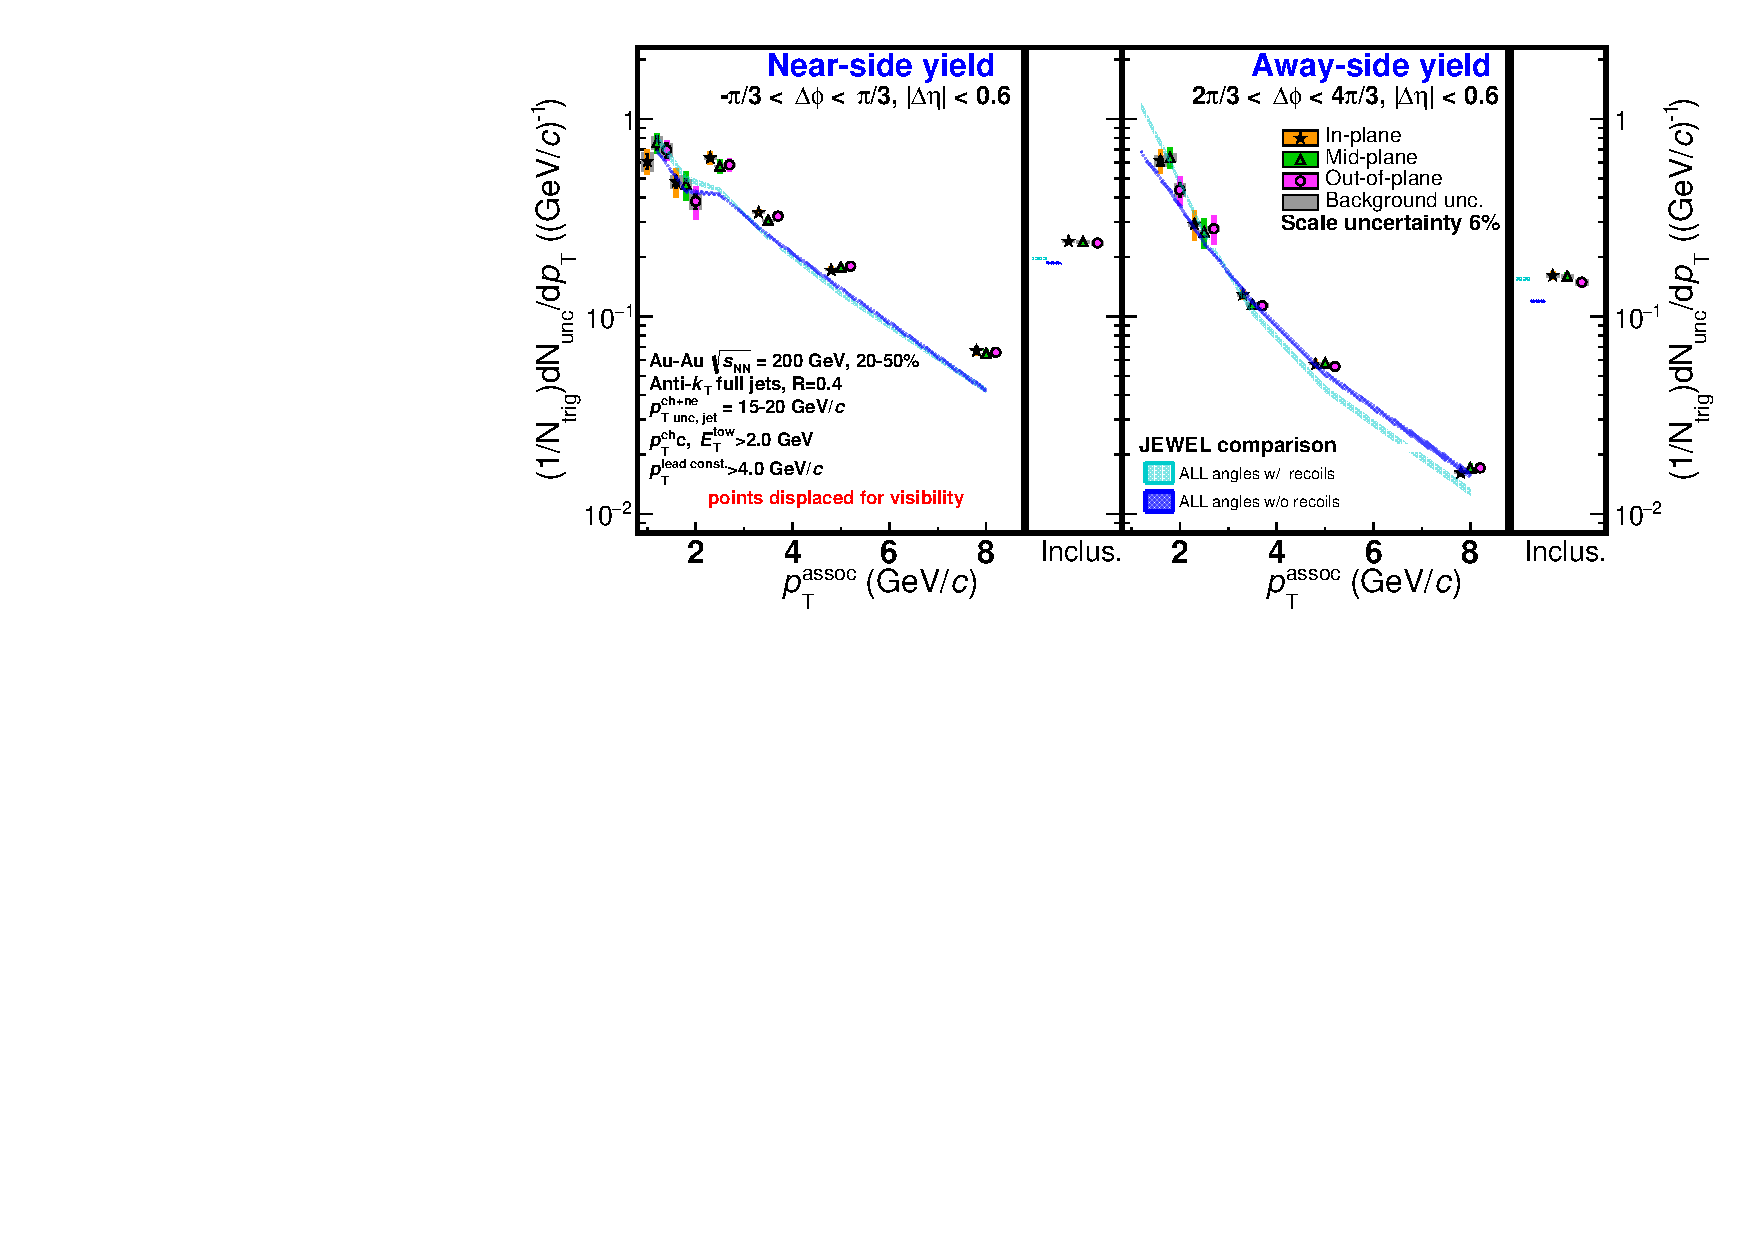
\includegraphics[width=\linewidth]{figures/JHC/results/NearAwaySideYield_J15-20_C20-50_wJEScorr_wJEWELerr.pdf}
		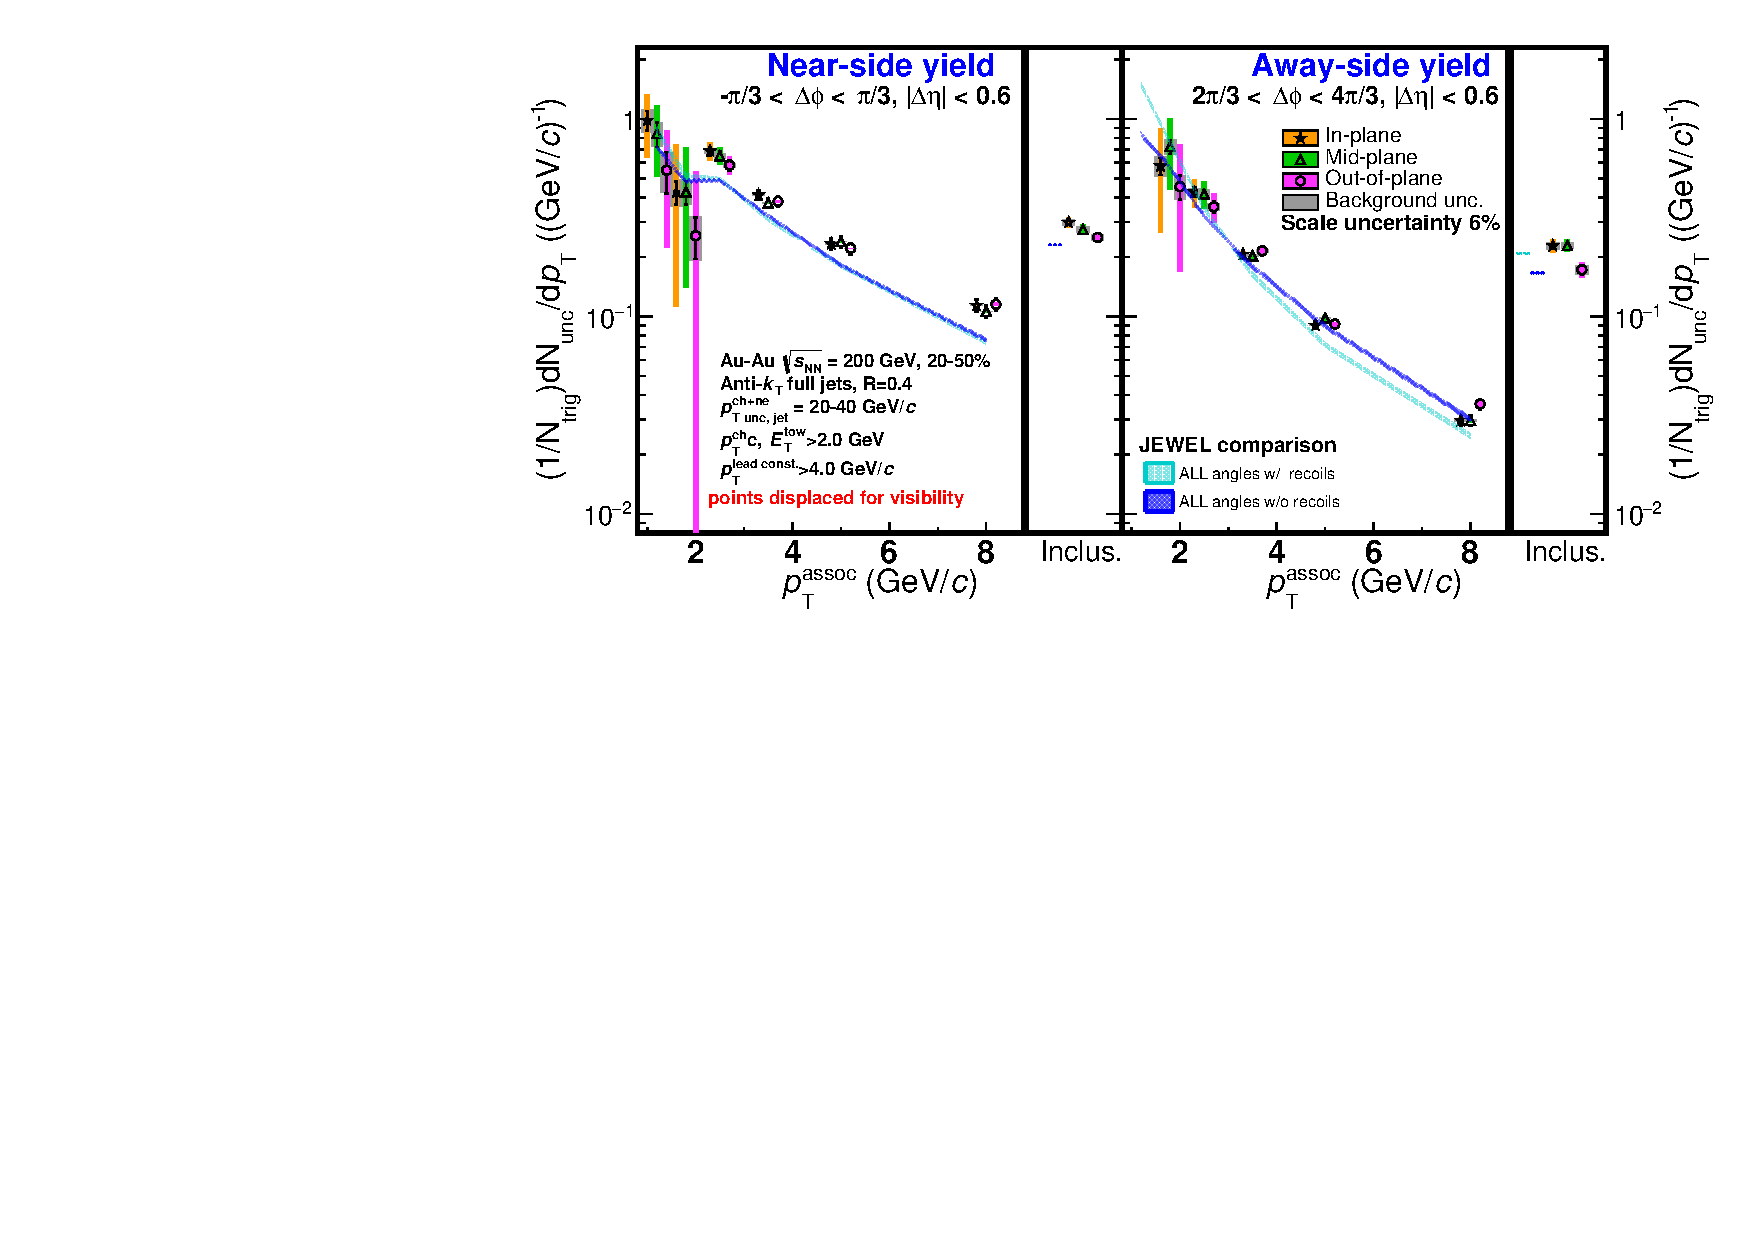
\includegraphics[width=\linewidth]{figures/JHC/results/NearAwaySideYield_J20-40_C20-50_wJEScorr_wJEWELerr.pdf}
		\caption[Near- and away-side associated yields as functions of \(p_\mathrm{T, assoc}\)]{Near-side (left) and away-side (right) uncorrected (unc.) associated yield vs \Pt{assoc} for 15--20 (top) and 20--40~\GeVc (bottom) full jets of 20--50\% centrality in \AuAu collisions.  The gray bands describe the systematic uncertainties of the background fits and are non-trivially correlated point-to-point.  The colored bands are scale uncertainties from the mixed-event acceptance shape and JES correction.  There is an additional 6\% global scale uncertainty.  Included on the far right of the near- and away-side panels is the inclusive transverse momentum bin from 1.0--10.0~\GeVc.  Points are displaced for visibility. } 
		\label{fig:AssocYields}
	\end{center}
\end{figure}

\label{sect:Widths}
The widths are calculated by fitting a Gaussian, $A\,\mathrm{e}^{-(\Delta\phi - \Delta\phi_0)^2/2\sigma^2}$, to the jet peak centered at $\dphi_0 = 0$ for the near-side and $\dphi_0 = \pi$ for the away-side.  The Gaussians are fitted separately, with a range of $|\Delta\phi|~<~\pi/3$ on the \ns and $|\Delta\phi - \pi|~<~\pi/3$ on the \as. The Gaussian fit is repeated with different values of the background parameters and the covariance matrix is used to propagate the uncertainties.  The scale uncertainties on the widths are given by $\sigma_{w}^{sc} = \frac{B}{\sigma_B} \times |\alpha - 1|$, where $\alpha$ (Eq.~\ref{Eqtn:alpha}) is the \Pt{assoc}-dependent scale factor associated with the acceptance shape when propagating the background determined in the $0.6 \leq |\deta| < 1.2$ to the region $|\deta| < 0.6$.  

Fig.~\ref{fig:JetWidths} shows that the jet peaks broaden with decreasing \Pt{assoc}.  This is expected from both collisional energy loss and gluon bremsstrahlung.  With out-of-plane jets expected to traverse a longer average path length than in-plane jets, this would lead to additional interactions with the medium and more subsequent re-scatterings resulting in a larger width for jets out-of-plane relative to in-plane.   Within the uncertainties there is no clear ordering.  This indicates the effect of path-length dependent energy loss is not large enough to be seen by the current precision of the data.  On the far right of the near- and away-side panels is the inclusive \Pt{assoc} bin with \ptassocrange{1.0}{10}.   The widths of each event-plane orientation in the inclusive selection for the sample with \pttrigrange{15}{20} are consistent.  Conversely, the \pttrigrange{20}{40} sample reveals indications of potential modifications.
This potential modification is apparent on both the near- and away-side and primarily comes from the lowest transverse momentum bins where sample size is the largest.

\begin{figure}
	\begin{center}     
		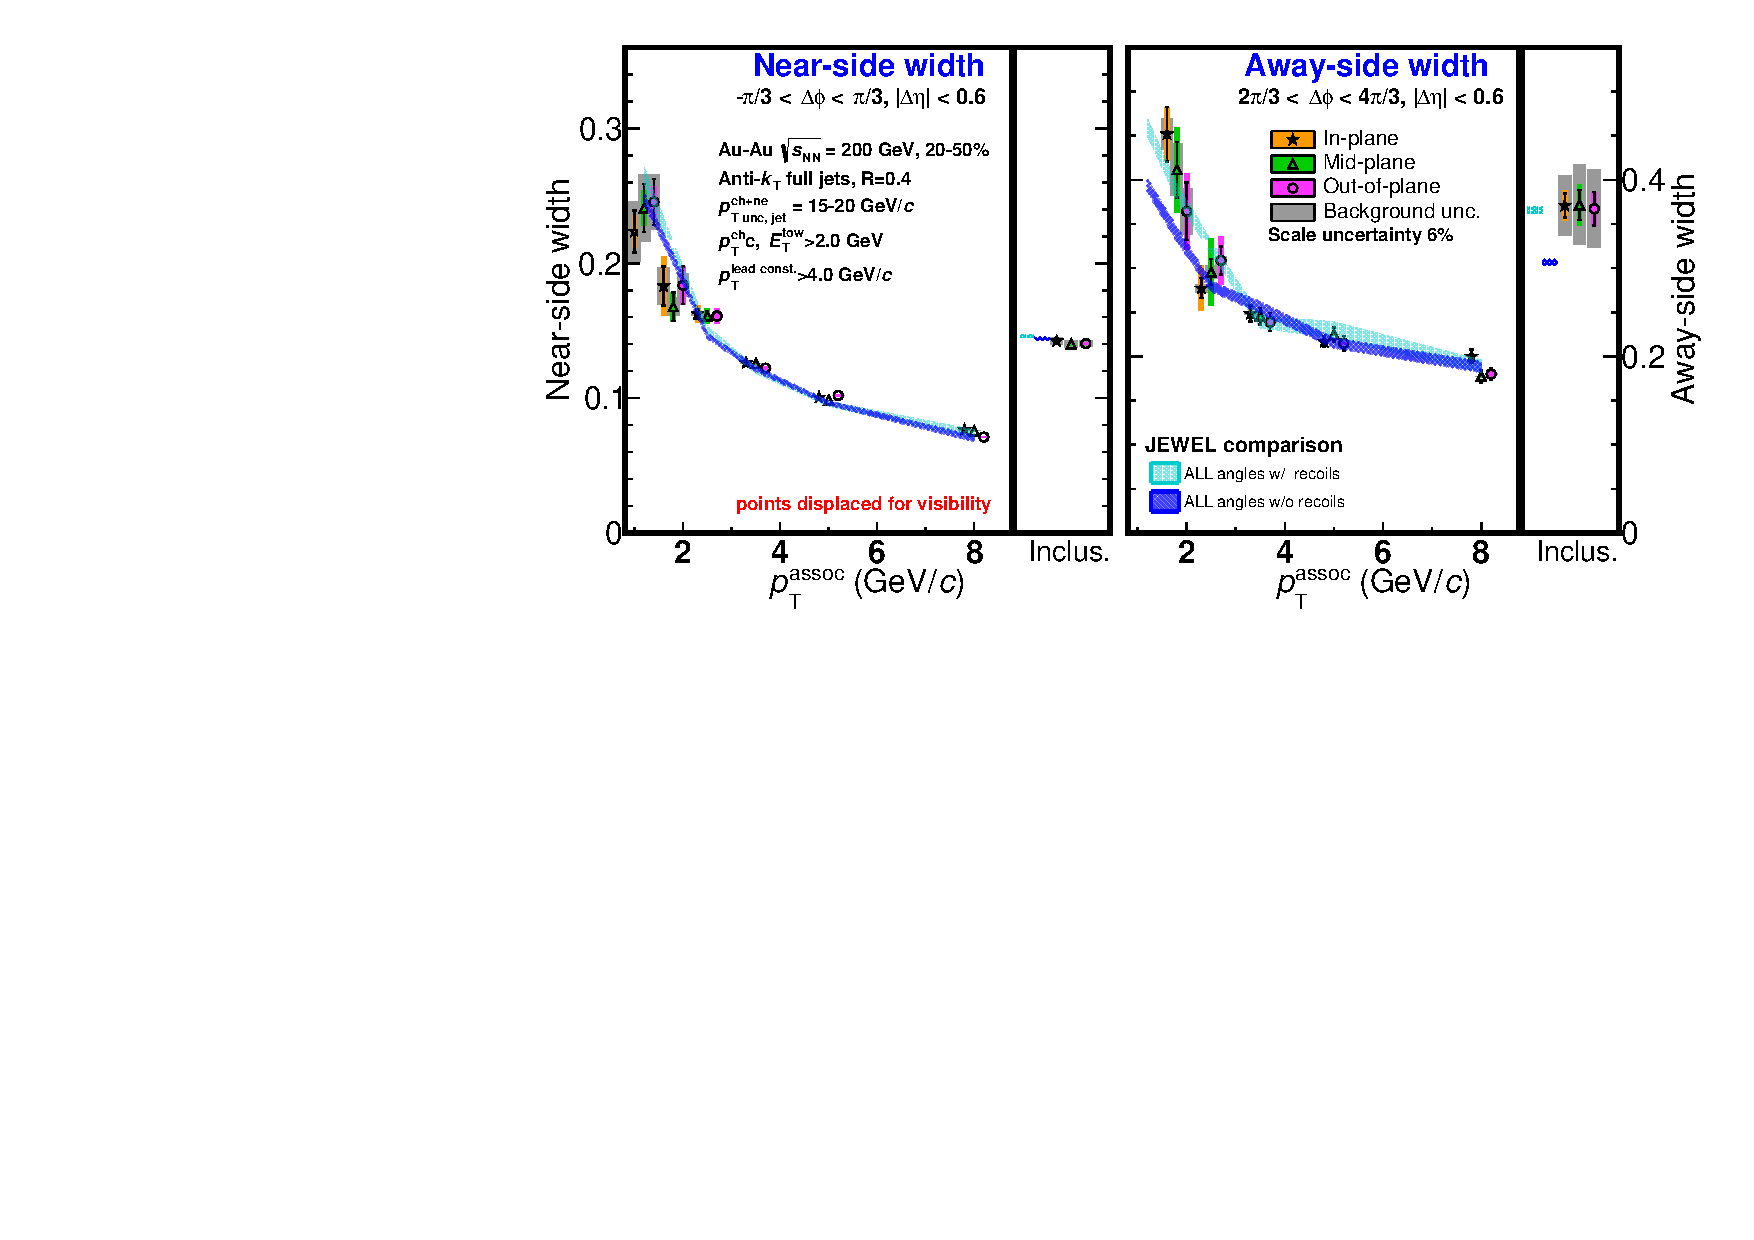
\includegraphics[width=\linewidth]{figures/JHC/results/NearAwaySideWidths_J15-20_C20-50_wJEScorr_wJEWELerr.pdf}
		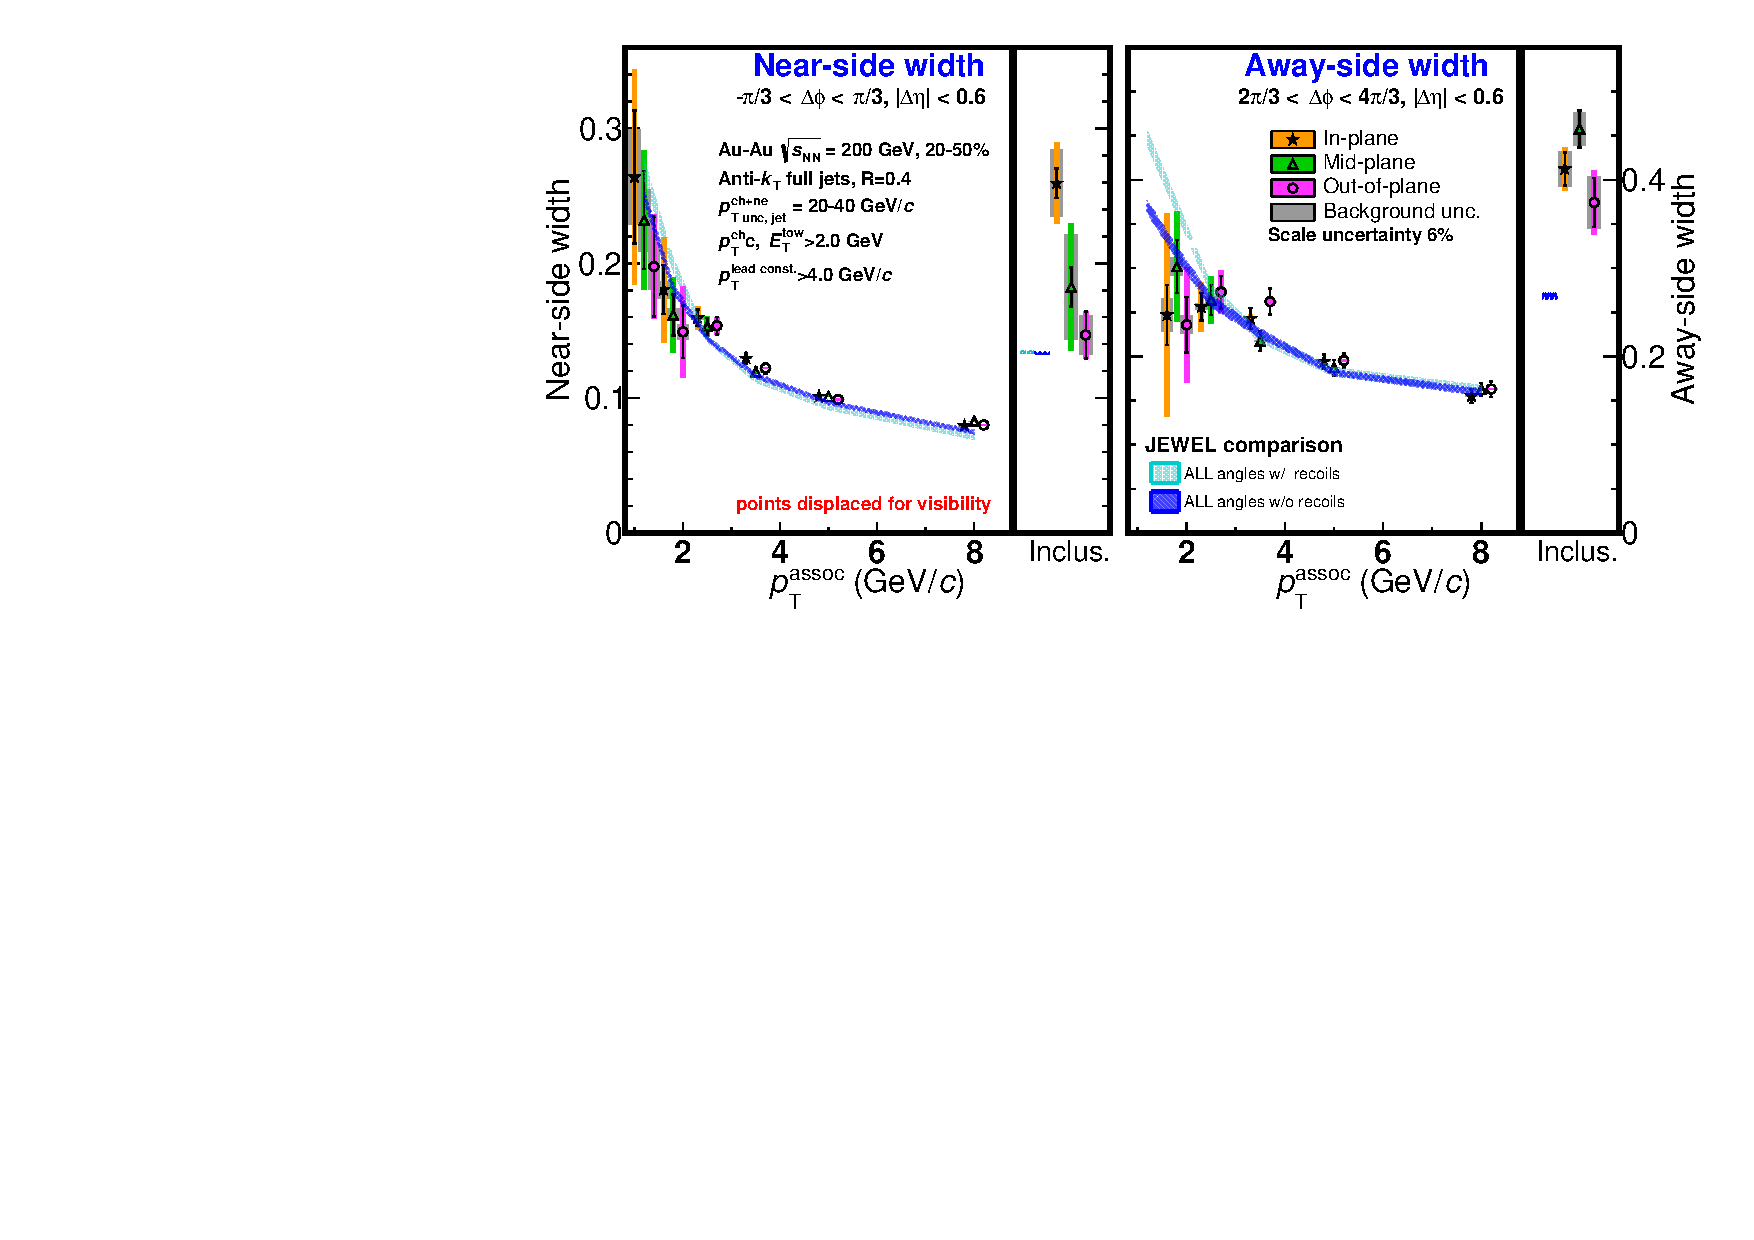
\includegraphics[width=\linewidth]{figures/JHC/results/NearAwaySideWidths_J20-40_C20-50_wJEScorr_wJEWELerr.pdf}
		\caption[Near- and away-side jet-peak widths as functions of \(p_\mathrm{T, assoc}\)]{Near-side (left) and away-side (right) jet width vs \Pt{assoc} for 15--20 (top) and 20--40~\GeVc (bottom) full jets of 20--50\% centrality in \AuAu collisions.  The widths are extracted from the Gaussian fit to the jet peak.  The gray bands describe the systematic uncertainties of the background fits which are non-trivially correlated point-to-point.  The colored bands are scale uncertainties from the mixed-event acceptance shape and JES correction.  There is an additional 6\% global scale uncertainty.  Included on the far right of the near- and away-side panels is an inclusive transverse momentum bin from 1.0--10.0~\GeVc.  Points are displaced for visibility. }
		\label{fig:JetWidths}
	\end{center}
\end{figure}

The measurements presented in Figs.~\ref{fig:AssocYields} and~\ref{fig:JetWidths} are compared to calculations from JEWEL introduced in Sec.~\ref{sec:eventGenerators}, with and without the recoil partons kept in the event. Without recoils, the momentum lost by the jet leaves the event, which models the energy loss of the hard part of the jet; with recoils, the momentum of the jet is conserved, but the recoils also add energy and particles to the dijet, and an experimental analysis likely measures some, but not all, of them, as they are often indistinguishable from the background.

Due to the dominant impact of jet-by-jet fluctuations on partonic energy loss over path-length dependence~\cite{Milhano:2015mng,Zapp:2013zya}, JEWEL only predicts a very slight event-plane dependence which is well below the systematic uncertainty in the measurement.  Variations among event-plane orientations were not seen at the 10\% level.  This is therefore consistent with path-length dependence having an insignificant impact compared to jet-by-jet fluctuations in energy loss.  Fluctuations in the density of the medium may also suppress observable path-length dependence and are not included in the JEWEL model.  However,  higher precision JEWEL calculations may be needed to discern any potential event-plane dependent effects.  The JEWEL comparisons are therefore shown for the sample integrated over all angles relative to the event plane and compared to the results from data, so that the event-plane resolution does not enter the comparison.  Comparisons show that the away-side is well described in terms of both the associated yields and widths by including recoils at low \Pt{assoc}, while at high \Pt{assoc}, the yields are better described by not including recoils and the widths have similar results to within uncertainties for both cases.  When looking at the near-side, the widths are quite similar at high \Pt{assoc} with slightly larger values when including recoils at low \Pt{assoc}.  For the associated yields at high \Pt{assoc}, both JEWEL cases are similar to each other, but underestimate the data and including recoils has larger yields that better match the data at low \Pt{assoc}.

\label{sect:YieldRatio}
To better quantify and examine the event-plane dependence of the yields, ratios were taken of mid-plane yields relative to in-plane yields and out-of-plane yields relative to in-plane yields.  The advantage of taking ratios is a reduction in systematic uncertainties due to cancellation of uncertainties from several sources.  The propagation of uncertainties follows Sec.~\ref{sect:RPF}.  The yield ratio is expressed as:

\begin{equation}
	r = \frac{Y_A}{Y_B} = \frac{Y_A^{\rm meas} - Y_A^{\rm bkgd}}{Y_B^{\rm meas} - Y_B^{\rm bkgd}},
	\label{eqn:YieldRatio}
\end{equation}

\noindent where A and B denote different event-plane orientations of the yield.  The statistical uncertainties, which come only from the completely uncorrelated terms $Y_A^{\rm meas}$ and $Y_B^{\rm meas}$, are calculated as: 

\begin{equation}
	\sigma^{\rm stat}_r = \left|\frac{1}{r}\right|\sqrt{\left(\frac{\sigma_A}{Y_A}\right)^2 + \left(\frac{\sigma_B}{Y_B}\right)^2}.
	\label{eqn:StatRatio}
\end{equation}

\noindent The scale uncertainties, displayed as colored bands on the yield and width plots, are correlated and completely cancel in the ratio.  Uncertainties from the RPF background subtraction are propagated with Eq.~\ref{eqn:CovProp}, but now applied to Eq.~\ref{eqn:YieldRatio}, which includes correlated background terms in the numerator and denominator of the ratio, so that part of the background uncertainty cancels.  The correlated background uncertainties are given by:

\begin{equation}
	\sigma^{\rm bkgd}_r = \sqrt{\sum_{i=0}^{N} \sum_{j=0}^{N} \frac{\partial r}{\partial p_i} \frac{\partial r}{\partial p_j} \sigma_{ij}}.
	\label{eqn:SysRatio}
\end{equation}

Where, $p_i$'s are the parameters of the RPF fits. Fig.~\ref{plot:YieldRatio_C20-50} shows the near-side (left) and away-side (right) associated-yield ratios of out-of-plane/in-plane and mid-plane/in-plane for 15--20 (top) and 20--40~GeV/\(c\) (bottom) jets.
%
The ratios are not corrected for the finite event-plane resolution (Sec.~\ref{sec:EPReco}): a real difference between the orientations would appear in them reduced to about half of its size.

For \pttrigrange{15}{20}, the out-of-plane to in-plane associated-yield ratio shows slight enhancement out-of-plane relative to in-plane at low \Pt{assoc}, although the effect is small.  This can potentially be due to additional induced gluon radiation that out-of-plane and mid-plane jets would experience relative to in-plane jets, possibly from the longer path length traversed by jets that are not in-plane.   Deviations of the yield ratios from 1.0 are not statistically significant on the away-side, although a small suppression is seen in-plane relative to both mid-plane and out-of-plane on both the near-side and the away-side for \ptassocrange{2.0}{5.0} for out/in.  The suppression is expected to occur at a higher momentum fraction ($z$) of the jet.  On the away-side, the effects are favoring a redistribution of energy from high-momentum constituents to lower momentum constituents.  
%However, the away-side measurement is not sensitive enough to the potential effects because the uncertainties associated with the result are dominated by both the statistics and the JES correction.
%the shift in energy to reconstructed jets from varying $v^{jet}_2$ between event-plane orientations.

For \pttrigrange{20}{40} the near-side ratios are consistent with 1.0 with some movement at the two lowest \Pt{assoc} bins.  On the away-side, mid/in is consistent with 1.0 with a little enhancement and out/in has an enhancement at high \Pt{assoc} and suppression at low \Pt{assoc}. This observation contradicts the expectations.  If in-plane jets interact less, the ratios are expected to be $< 1.0$ at high \Pt{assoc} and $> 1.0$ at low \Pt{assoc}.  This is a reminder of the competing effects in the analyzed momentum range, and it is an indication that the expected path-length effects due to jet energy loss are dominated by the fluctuations in the medium.

%\begin{figure}[!htbp]
\begin{figure}
	\begin{center}     
		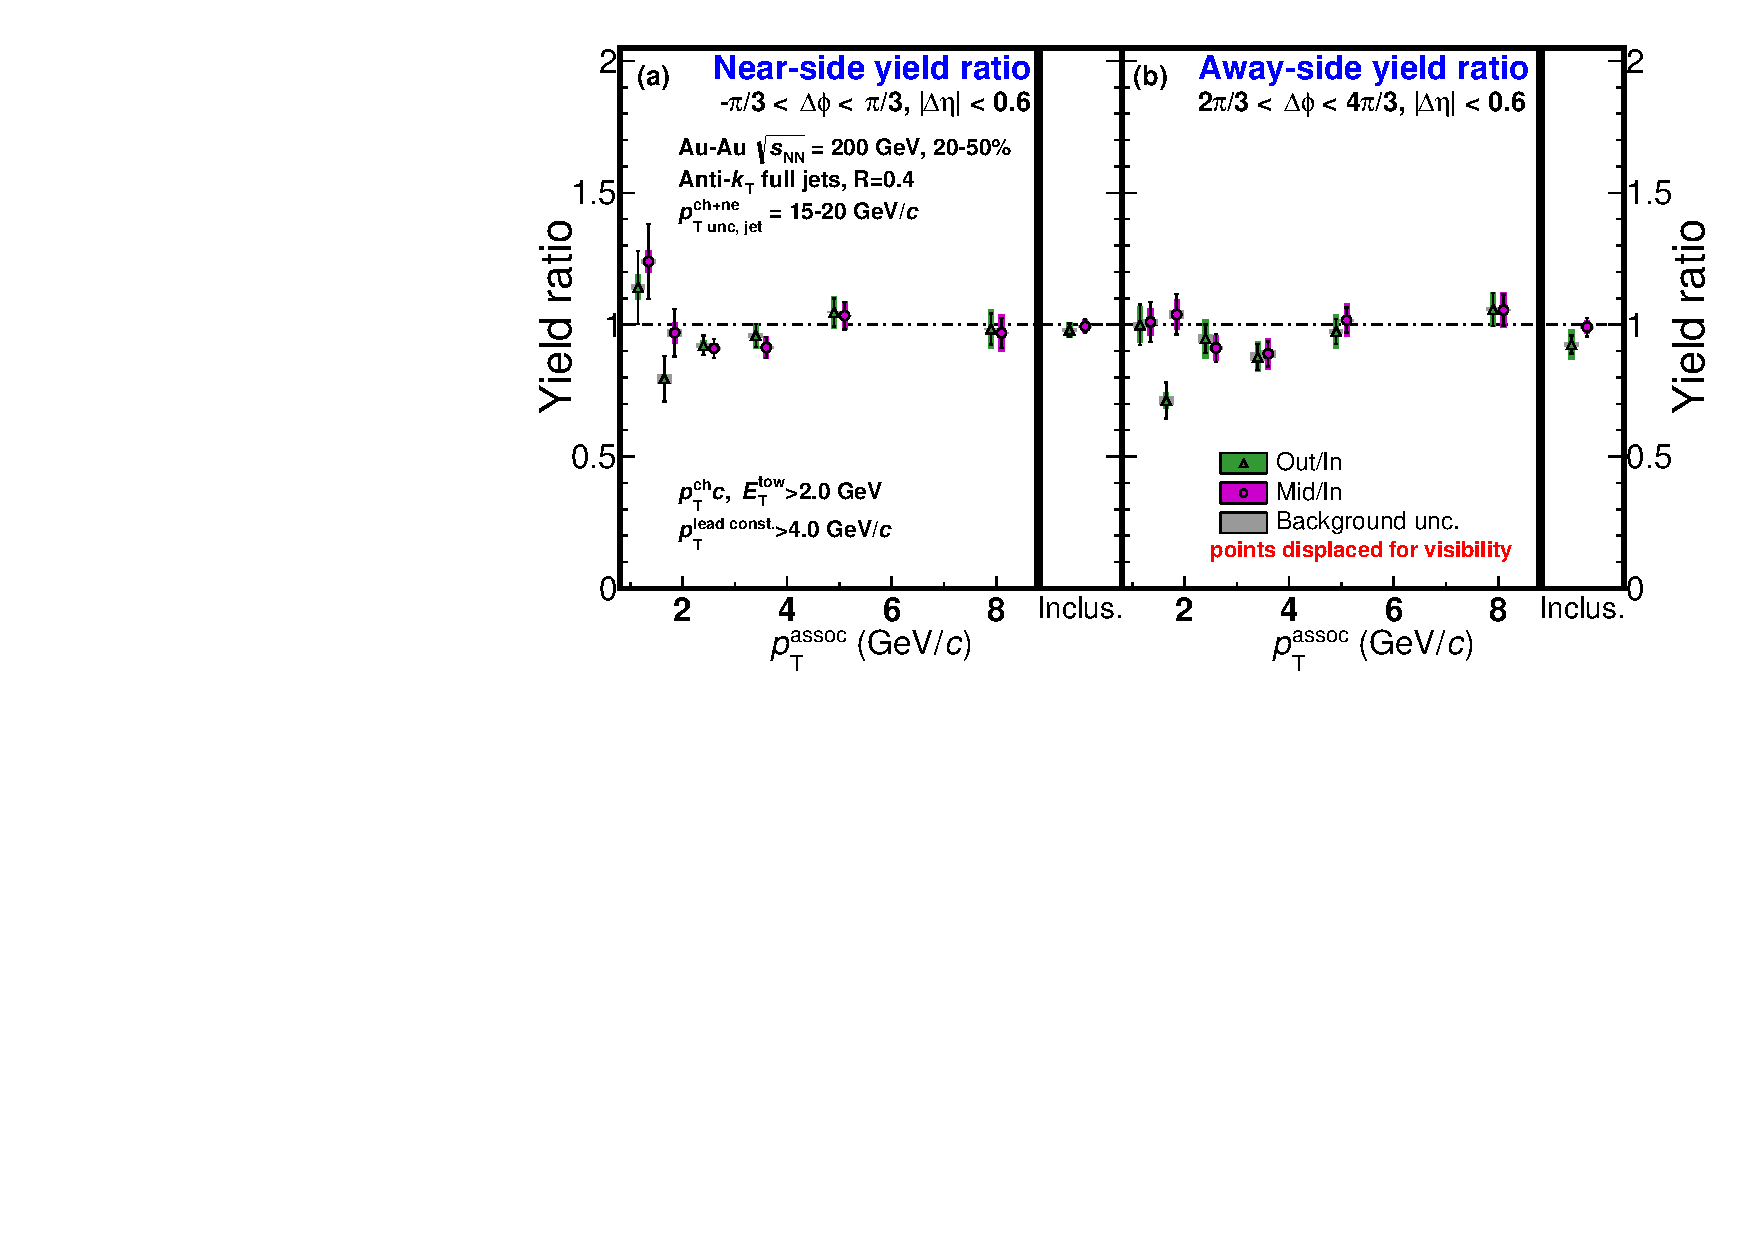
\includegraphics[width=\linewidth]{JHC/results/YieldRatio_J15-20_C20-50_wJEScorr.pdf}
		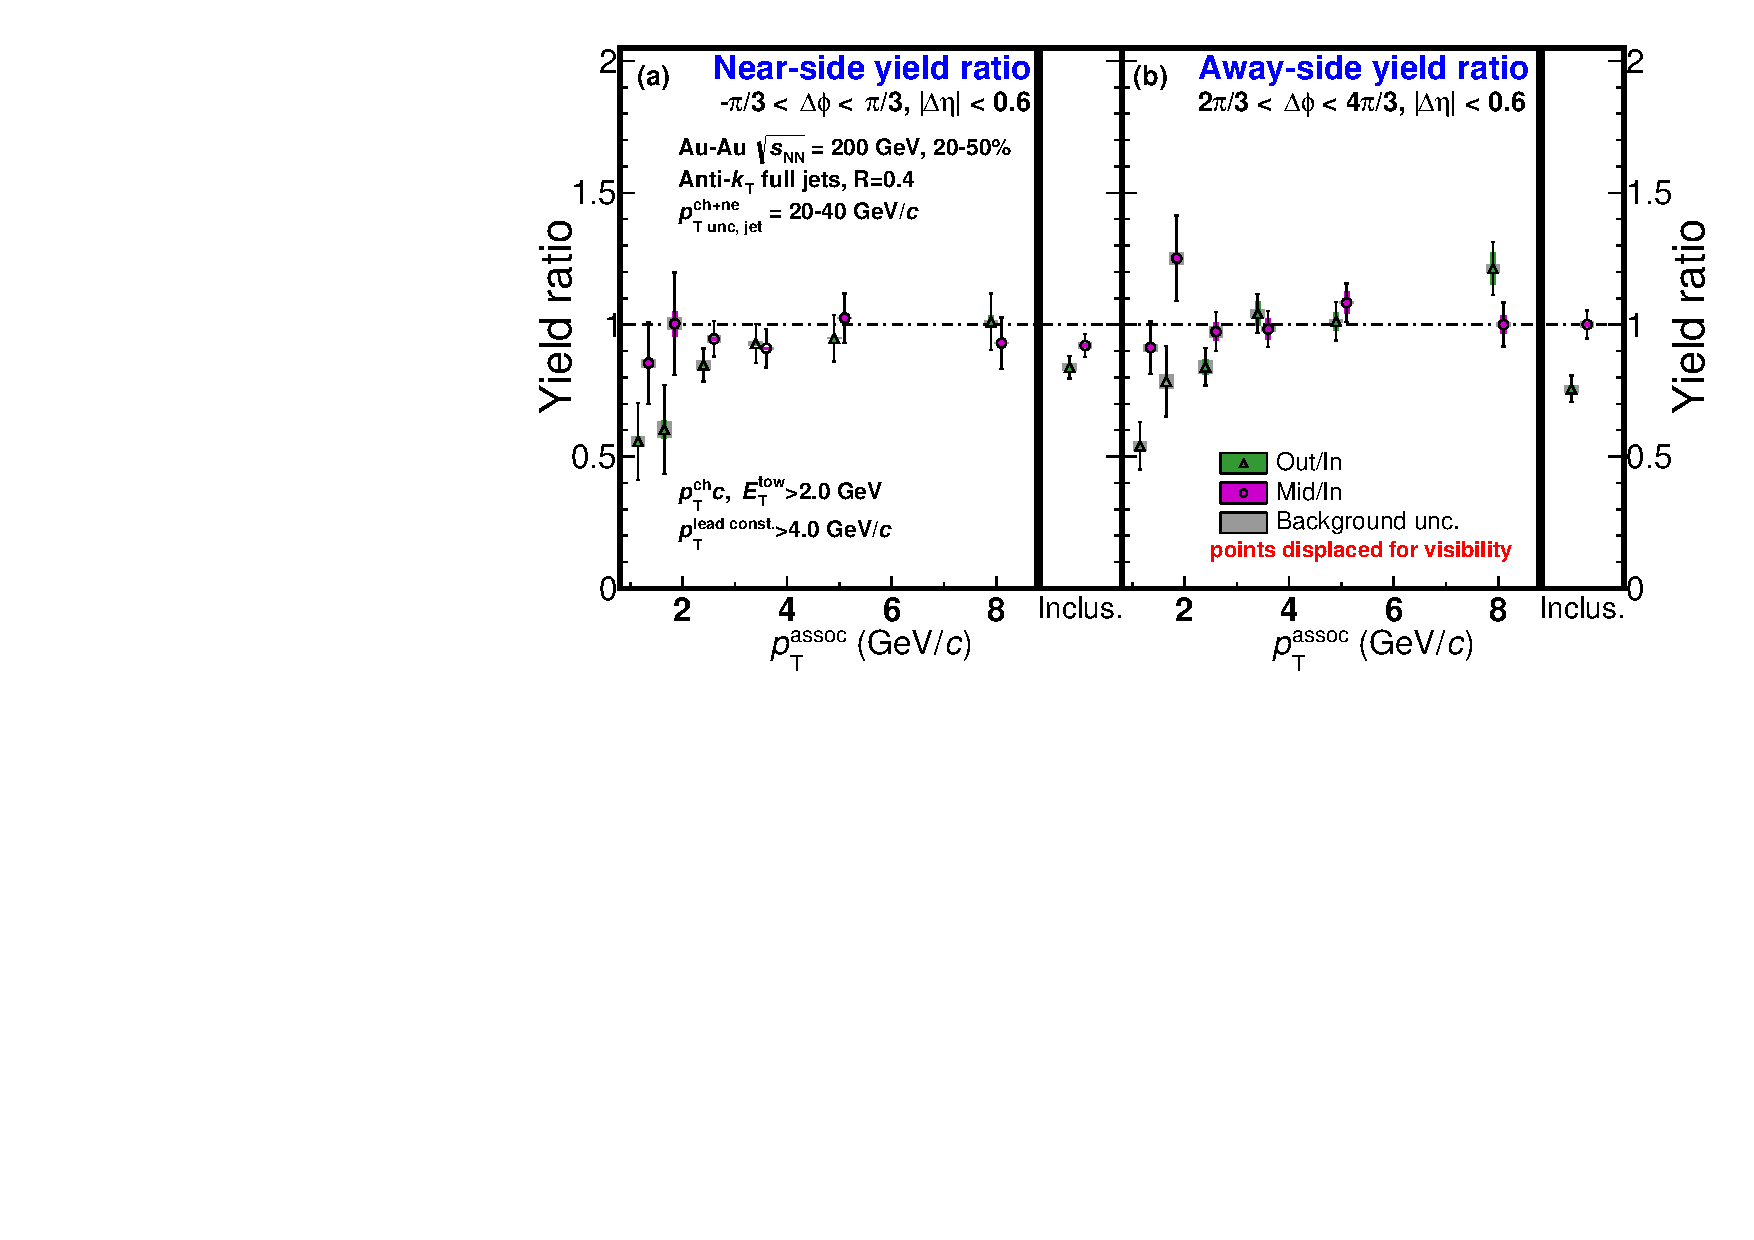
\includegraphics[width=\linewidth]{JHC/results/YieldRatio_J20-40_C20-50_wJEScorr.pdf}
		\caption[Out-of-plane/in-plane and mid-plane/in-plane associated-yield ratios]{Near-side (left) and away-side (right) associated-yield ratios (of out-of-plane and mid-plane to in-plane) vs \Pt{assoc} for 15--20 (top) and 20--40 (bottom)~GeV/\(c\) full jets in 20--50\% centrality collisions.  The gray bands describe the systematic uncertainties of the background fits which are non-trivially correlated point-to-point.  The colored bands are scale uncertainties from the JES correction.  Points are displaced for visibility. }
		\label{plot:YieldRatio_C20-50}
	\end{center}
\end{figure}

Alternatively, the initial geometry within specific centrality bins may be fluctuating at a larger magnitude than any possible event-plane dependence~\cite{Noronha-Hostler-RAAv2,PhysRevLett.116.252301}.  The possibility of this occurrence can be studied by looking at the initial configuration and selecting low and high ellipticity events by  using the $q_n$ flow vector found within a selected centrality range.  Since the present measurement is already limited by statistics, such a selection, which keeps only a fraction of the events, would require the larger \AuAu datasets recorded by STAR in 2023 and 2025~\cite{RHICRunSummary}.

To study the impact of surface bias and event-plane resolution, a check was performed to investigate the systematic change in the ratio of yields (out/in, mid/in) with the angle of the event plane by fitting a constant to Fig.~\ref{plot:YieldRatio_C20-50} for jets with \pttrigrange{15}{20} (top) and \pttrigrange{20}{40} (bottom).  The systematic uncertainties are treated as uncorrelated point-to-point and added to the statistical uncertainties in quadrature.  The results are shown in Tabs.~\ref{Tab:RatioFits_J15-20} and~\ref{Tab:RatioFits_J20-40} and are consistent with one.  Care should be taken when interpreting the results, as various effects can be in play and medium modifications could give way to a \Pt{assoc} dependence. This \Pt{assoc} dependence can be seen as an enhancement of associated yields for $\Pt{assoc} \geq$ 2 \GeVc on the near-side from the geometric kinematic biases due to the ``hard-core'' requirement of jet reconstruction.   

%======================================================================
\begin{table}
	%\begin{table}[!ht]
	\caption[Constant fits to the associated-yield ratios for 15--20~GeV/\(c\) jets]{Results of fits to Fig.~\ref{plot:YieldRatio_C20-50} (top panel: 15--20~\GeVc jets) to a constant $c$, the $\chi^2$ over the number of degrees of freedom (NDF), the number of standard deviations $\sigma$ of $c$ from one, and the range of $c$ within a 90\% confidence limit (CL).}
	\label{Tab:RatioFits_J15-20}
	\centering % used for centering table
	\begin{tabular}{c | c c | c c} % entered columns (5 columns)
		\hline
		& \multicolumn{2}{c |}{Near-side}  & \multicolumn{2}{c}{Away-side}  \\
		parameter & $Y_{\mathrm{out}} / Y_{\mathrm{in}}$  & $Y_{\mathrm{mid}} / Y_{\mathrm{in}}$   & $Y_{\mathrm{out}} / Y_{\mathrm{in}}$  & $Y_{\mathrm{mid}} / Y_{\mathrm{in}}$  \\ \hline
		%XXX OLD
		%$c$ &  0.977 $\pm$  0.026 &  0.999 $\pm$  0.029 &  0.885 $\pm$  0.028 &  0.965 $\pm$  0.032 \\
		%$\chi^2$/NDF &  1.8  & 0.41  & 0.98 & 0.63 \\
		%$\sigma$ & -0.9 & -0.0 & -4.1 & -1.1 \\
		%90\% CL & 0.91 -- 1.05 & 0.96 -- 1.04 & 0.83 -- 0.94 & 0.91 -- 1.02 \\
		% ---- before JES Shift correction ----
		%$c$          & 0.949 $\pm$ 0.02 & 0.983 $\pm$ 0.019 & 0.914 $\pm$ 0.023 & 0.979 $\pm$ 0.022 \\
		%$\chi^2$/NDF & 3.4              & 0.35              & 3                 & 0.39 \\
		%$\sigma$     & -2.6             & -0.9              & -3.7              & -1.0 \\
		%90\% CL      & 0.88 -- 1.02     & 0.96 -- 1.01      & 0.83 -- 0.99      & 0.95 -- 1.01 \\
		$c$          & 0.93 $\pm$ 0.042 & 0.949 $\pm$ 0.038 & 0.89 $\pm$ 0.065 & 0.997 $\pm$ 0.066 \\
		$\chi^2$/NDF & 0.68             & 0.67              & 0.71             & 0.18 \\
		$\sigma$     & -1.6             & -1.3              & -1.7             & -0.1 \\
		90\% CL      & 0.86 -- 1.00     & 0.89 -- 1.01      & 0.78 -- 1.00     & 0.94 -- 1.05 \\
		\hline
	\end{tabular}
\end{table}

%======================================================================
% === Comment out table for 20-40 GeV jets, ====
\begin{table}
	%\begin{table}[!ht]
	\caption[Constant fits to the associated-yield ratios for 20--40~GeV/\(c\) jets]{Results of fits to Fig.~\ref{plot:YieldRatio_C20-50} (bottom panel: 20--40~\GeVc jets) to a constant $c$, the $\chi^2$ over the number of degrees of freedom (NDF), the number of standard deviations $\sigma$ of $c$ from one, and the range of $c$ within a 90\% confidence limit (CL).}
	\label{Tab:RatioFits_J20-40}
	\centering % used for centering table
	\begin{tabular}{c | c c | c c} % entered columns (5 columns)
		\hline
		& \multicolumn{2}{c |}{Near-side}  & \multicolumn{2}{c}{Away-side}  \\
		parameter & $Y_{\mathrm{out}} / Y_{\mathrm{in}}$  & $Y_{\mathrm{mid}} / Y_{\mathrm{in}}$   & $Y_{\mathrm{out}} / Y_{\mathrm{in}}$  & $Y_{\mathrm{mid}} / Y_{\mathrm{in}}$  \\ \hline
		%XXX OLD
		% $c$ &  0.921 $\pm$  0.042 &  0.998 $\pm$  0.053 &   1.06 $\pm$  0.047 &    1.1 $\pm$   0.05 \\
		% $\chi^2$/NDF & 0.36  & 0.73  &  3.9 & 0.43 \\
		% $\sigma$ & -1.9 & -0.0 & 1.2 & 2.0 \\
		% 90\% CL & 0.87 -- 0.97 & 0.91 -- 1.09 & 0.87 -- 1.24 & 1.03 -- 1.17 \\
		% --- before JES Shift correction ---
		%$c$          & 0.898 $\pm$ 0.032 & 0.969 $\pm$ 0.033 & 0.989 $\pm$ 0.035 & 1.04 $\pm$ 0.033 \\
		%$\chi^2$/NDF & 0.84              & 0.44              & 3.6               & 1.5 \\
		%$\sigma$     & -3.2              & -1.0              & -0.3              & 1.3 \\
		%90\% CL      & 0.84 -- 0.96      & 0.93 -- 1.01      & 0.86 -- 1.12      & 0.96 -- 1.13 \\
		$c$          & 0.874 $\pm$ 0.043 & 0.937 $\pm$ 0.043 & 0.752 $\pm$ 0.064 & 1.02 $\pm$ 0.075 \\
		$\chi^2$/NDF & 1.4               & 0.19              & 2.1               & 0.49 \\
		$\sigma$     & -2.9              & -1.5              & -3.9              & 0.2 \\
		90\% CL      & 0.77 -- 0.98      & 0.90 -- 0.97      & 0.56 -- 0.94      & 0.91 -- 1.12 \\
		\hline
	\end{tabular}
\end{table}

\section{Conclusions} \label{sect:Summary}
The measurement of jet-hadron correlations relative to the event plane is reported for the 20--50\% most central events in \AuAu collisions at \sNN{200}{GeV} in STAR. 
%
Partonic interactions are directly related to the distance traversed in the medium, so it is expected that medium-induced jet modifications should depend on the path length. 
%
The angle of the jet, measured with respect to the event plane, is correlated on average with the jet's path length through the medium. 
%
In this analysis, the average path length of away-side jets is potentially increased due to the surface bias of the near-side trigger jet. 
%
This work utilizes the RPF background-subtraction method to remove the event-plane dependent background while reducing uncertainties and assumptions associated with previous background-subtraction techniques. 
%
Associated yields, their ratios, and jet-peak widths are extracted for each event-plane orientation and compared with different average path lengths and JEWEL model calculations. 
%
JEWEL performs better in describing the associated yields and widths at higher \Pt{assoc} when recoil partons are not included. 
%
Conversely, including recoil partons leads to JEWEL providing a better description of the lower \Pt{assoc} region. 
%
This study highlights the importance of conducting further tuning of Monte Carlo simulations to accurately describe the results in this analysis for jets that are biased towards hard-fragmented jets due to the HT-trigger and hard-core constituent requirements.

Within the precision of the current measurement at \sNN{200}{GeV}, the associated yields and jet-peak widths show no dependence on the event plane. 
%
The ratios derived from the associated yields are used to quantify the differences, but they do not deviate significantly from 1.0. For the \pttrigrange{20}{40} jets, there were indications of potential modifications observed in the inclusive bin of \ptassocrange{1.0}{10}.
%
The results presented in this study align with the findings observed in hadron-hadron and jet-hadron correlations reported in Ref.~\cite{Nattrass:2016cln} for RHIC and  Ref.~\cite{PhysRevC.101.064901} for LHC energies.  
%
The lack of clear event-plane dependence in the data indicates that any dependence of these modifications on the average path-length is less than the experimental uncertainties.
\chapter{Generalized Angularities}
\label{ch:angularities}
Substructure based observables calculated from constituents of clustered jets can potentially have sensitivity to variety of QCD processes, from initial hard (high-\(Q^2\)) parton scattering to hadronization.
%
Considering that, a constituent carries two major types of information, it's energy relative to the jet \(\left(z_\mathrm{const.} = \frac{p_{\rm T, const.}}{p_ {\rm T,  jet}}\right)\) and its direction with respect to the jet-axis, usually characterized by it's \(\eta-\varphi\) coordinate relative to the jet-axis \(\left(\Delta R_\mathrm{const., jet}=\sqrt{(\eta_\mathrm{const.} - \eta_\mathrm{jet})^2 + (\varphi_\mathrm{const.} - \varphi_\mathrm{jet})^2}\right)\).
%
An intuitive way to put these two information together is by raising \(z_\mathrm{const.}\) and \(\Delta R_\mathrm{const, jet}\) to exponents \(\kappa\) and \(\beta\) respectively and multiplying them. 
%
That would give bunch of per-constituent scalars, which we can add up  for a jet to get a family of jet observables called \emph{Generalized angularities}. 
%
\begin{equation}\label{eq:LambdaKappaBeta}
	\lambda_\beta^\kappa=\sum_{\mathrm{const} \in \mathrm{jet}}z_{\rm const.}^\kappa \left(\frac{\Delta R_\mathrm{const., jet}}{R}\right)^\beta
\end{equation}
%
The parameters $\kappa$ and $\beta$ provide tune experimental sensitivity to hard and wide-angle radiation, respectively. 
%
$\lambda^1_\beta$'s are IRC safe angularites~\cite{Berger_2003}, which probe the average angular spread of energy around the jet-axis. 
%
They are radial moments of the  jet's transverse momentum profile, also known as differential jet-shape (\(\rho(r)\)) given by Eq.~\ref{eq:rhoVsDr}.
%
Relating with \(e^+e^-\) collision measurements, \(\lambda_1^1\) is the jet \emph{width} or \emph{girth}~\cite{CATANI1992269} and \(\lambda_2^1\) is the jet \emph{thrust}~\cite{Thrust_Larkoski_2014}. 
%
Further, \(\lambda_2^1\) is related to the jet-mass~\((m_\mathrm{jet})\) as  \(\left(\lambda_2^1 = \frac{m^2_\mathrm{jet}}{p_\mathrm{T, jet}^2} + \mathbf{O}(()\lambda_2^1)^2) \right)\), providing an IRC-safe way of accessing \(m_\mathrm{jet}\) information as it doesn't directly depend on hadron masses.
%
\(\lambda_{0.5}^1\) was been shown to have sensitivity to initiating parton-type of the jet, called \emph{LHA angularity} after the Les Houches 2015 where the quark-gluon discrimination study was first shown~\cite{Andersen:2016qtm}.

As an experimental observable, it is useful to restrict the summation in Eq.~\ref{eq:LambdaKappaBeta} to only charged constituents / tracks and mitigate contamination from towers like pileup, especially in the case of heavy-ion collisions.  
%
This makes \(\lambda_{\beta > 0}^1\)  IRC unsafe, but as shown in~\cite{Chang_2013, ALICE:2021njq} comparison to theoretical predictions~\cite{Kang_2018, Kang:2018vgn} is still possible. 
%
Comparisons to theoretical predictions can be further simplified by disentangling the pQCD and npQCD contributions to the angularity, through use of grooming algorithms~\cite{Dasgupta_2013}. 

On the heavy-ion side, angularity measurements can help determine non-trivial biases introduced into nuclear modification factors. As shown in~\cite{Alice2018}, instead of observing expected effects like jet-broadening in central Pb+Pb collisions, an apparent narrowing effect is observed for small-area (\(R=0.2\)) jets.

Experimental measurements of IRC unsafe angularities like \(\lambda_0^0\), the jet-\emph{multiplicity} and \(\lambda_0^2\) jet-\emph{momentum dispersion} (\(= (p_T^D)^2\)) complement the \(\lambda_{\beta > 0}^1\)  with further information about jet fragmentation. 
%

In this chapter, various generalized angularites are measured at RHIC energies. 
%
These measurements explore jet fragmentation in a phase space of lower-momentum jets complimenting LHC measurements at high energies. 

\section{Angularities of Au+Au jets}
\label{sec:AuAuAngularities}
A brief exploratory analysis done on jets from the dataset used in chapter~\ref{ch:jhcorr} is shown. 
%
Distributions of Girth (\(g\)), \(p^D_T\), and LeSub given by, 
%
\begin{equation}
	\label{eq:AuAuJSODefs}
	\left(g,~p^D_T,~\text{LeSub}\right) \equiv \left(\lambda_1^1,~\sqrt{\lambda_0^2},~p_\mathrm{T, const.}^\mathrm{lead.} - p_\mathrm{T, const.}^\mathrm{sublead.}\right)
\end{equation}
%
LeSub is the \(p_\mathrm{T}\) difference between the leading and sub-leading constituents in the jet, which represents the split in momentum at the earliest fragmentation of the jet. 
%
The STAR preliminary results shown in this section were presented in the 30\(^\text{th}\) International Conference on Ultra-relativistic Nucleus-Nucleus Collisions (Quark Matter 2023)~\cite{Pani:2024mgy}. 

\subsection{Dataset and Selection}
Jets are reconstructed with same data (Au + Au collision from 2014), events (HT2-triggered, \(|v_z| < 24\)~cm; Sect.~\ref{sec:JHEventSel}), track and tower selection (Sect.~\ref{sec:TrackTowerSel}), constituents (hard-core,~\(cp_\mathrm{T, trk},~E_\mathrm{T, tow.} > 2.0\)~GeV)  and definition (\(R=0.4\),~anti-\(k_\mathrm{T}\),~boost-invariant \(p_\mathrm{T}^2\)) as in Sect.~\ref{sec:JetRecoAuAu}. 
%
The jet selection used in this analysis differs only  in that we omit the requirement for a high-tower triggered (\(E_\mathrm{T, tow.} \geq 5.4\)~GeV) inside the jet-cone and add an extra minimum jet-area cut \(A_\mathrm{jet} > 0.4\) to reduce combinatorial jet contribution.
%
The mathematical requirements to calculate the observables defined in Eq.~\ref{eq:AuAuJSODefs} further imposes a \(N_\mathrm{trk.} \geq 2\) selection on the jets. 

\subsection{Unfolding}
\begin{figure}
	\includegraphics[width=\linewidth]{angularities/AuAu/auau\_miss\_fake\_rates.pdf}
	\caption{Miss rate (left) and fake rate (right) calculated from matched jets from the PYTHIA-6 (STAR tune) + GEANT3 + AuAu 2014 minimum bias pedestal embedding simulation. Each panel shows the miss/fake rates for jets from 0-20\%, 20-40\%, and 40-80\%  centrality events as red circles, green squares, and blue triangles respectively.}
		\label{fig:AuAuMissAndFake}
\end{figure}
Residual background and detector effects are removed by mapping between particle and detector level jets using the embedding simulation and matching procedure described in section~\ref{sec:AuAuEmbedding}.
%
Efficiencies involved in jet reconstruction are shown in Fig.~\ref{fig:AuAuMissAndFake}.
%
A general decrease is seen in miss/fake rates going from smaller to larger \(p_\mathrm{T, jet}\)'s and from central to peripheral collisions.
%
The larger miss/fake rate in central and mid-central collisions (0-20\%,~20-40\%) can be explained by the presence of significant underlying event / minimum-bias pedestal compared to peripheral collisions (40-80\%).
%
MultiFold~\cite{PhysRevLett.124.182001} method was used to simultaneously unfold $p_{\rm T, jet}$, $\eta_{\rm jet}$, $\phi_{\rm jet}$, $N_{\rm cons, charged}$, \(g\), \(p_\mathrm{T}^\mathrm{D}\)~and LeSub. 
%
MultiFold uses Dense Neural Networks (DNNs) implemented using the EnergyFlow package~\cite{Komiske_2018},  which are trained on full embedding sample at the detector level and the generator level. 
%
See appendix~\ref{app:Unfolding} for more information about unfolding procedure and appendix~\ref{app:ML} for more information on machine learning.
%
Each classifier has three hidden layers of 100 nodes, and is trained with batches of 1024 jets on 80\% of the jets, the remaining 20\% being used for validation. Training is stopped once the validation loss has not improved for 10 epochs, and the network with the lowest validation loss is kept and used as the starting point in the next iteration.
%
The evolution of the losses during the unfolding is shown in Fig.~\ref{fig:multifoldTraining} for two runs with the nominal settings, since the training logs of the nominal runs themselves were not kept.
%
In step 1, the validation loss reaches its minimum within the first few epochs of each iteration while the training loss keeps decreasing, i.e. the classifier starts to learn fluctuations of the training sample, which the early stopping prevents from entering the weights. In step 2, the losses change little after the first epoch, as the reweighting between consecutive iterations is small.
\begin{figure}
	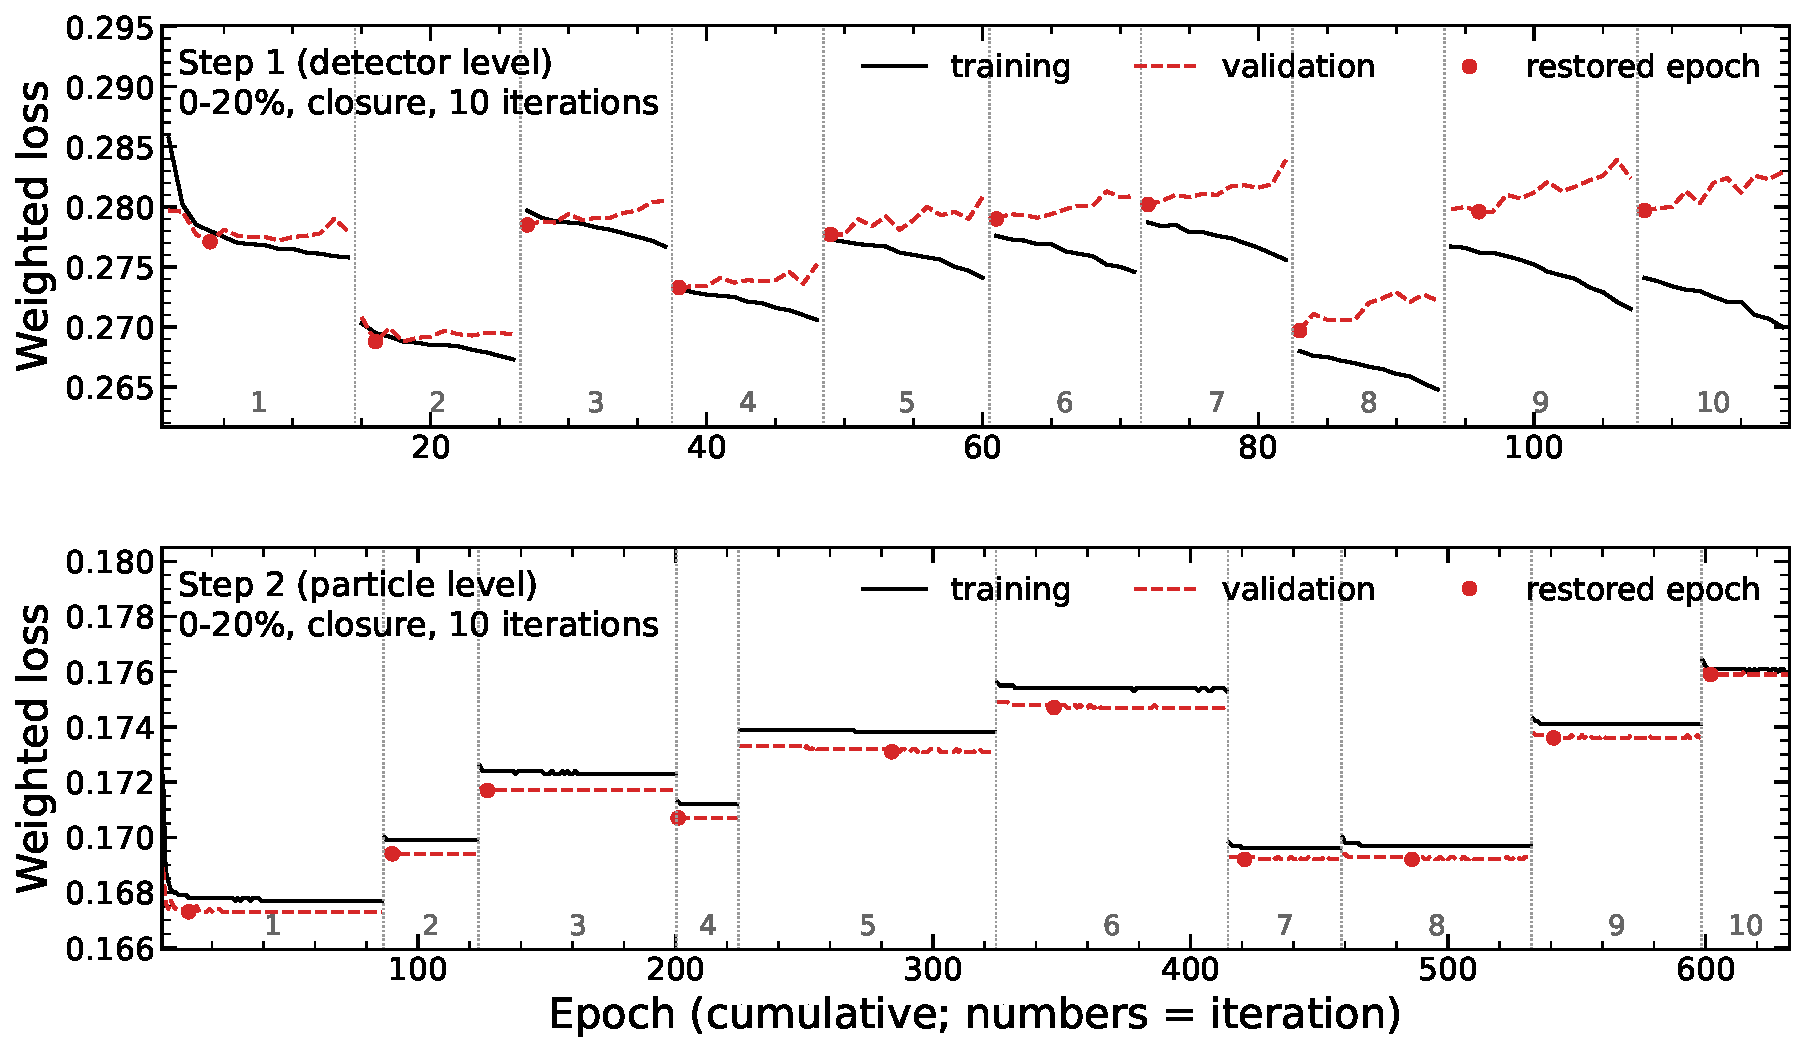
\includegraphics[width=\linewidth]{figures/angularities/AuAu/auau_training_0to20_closure.pdf}
		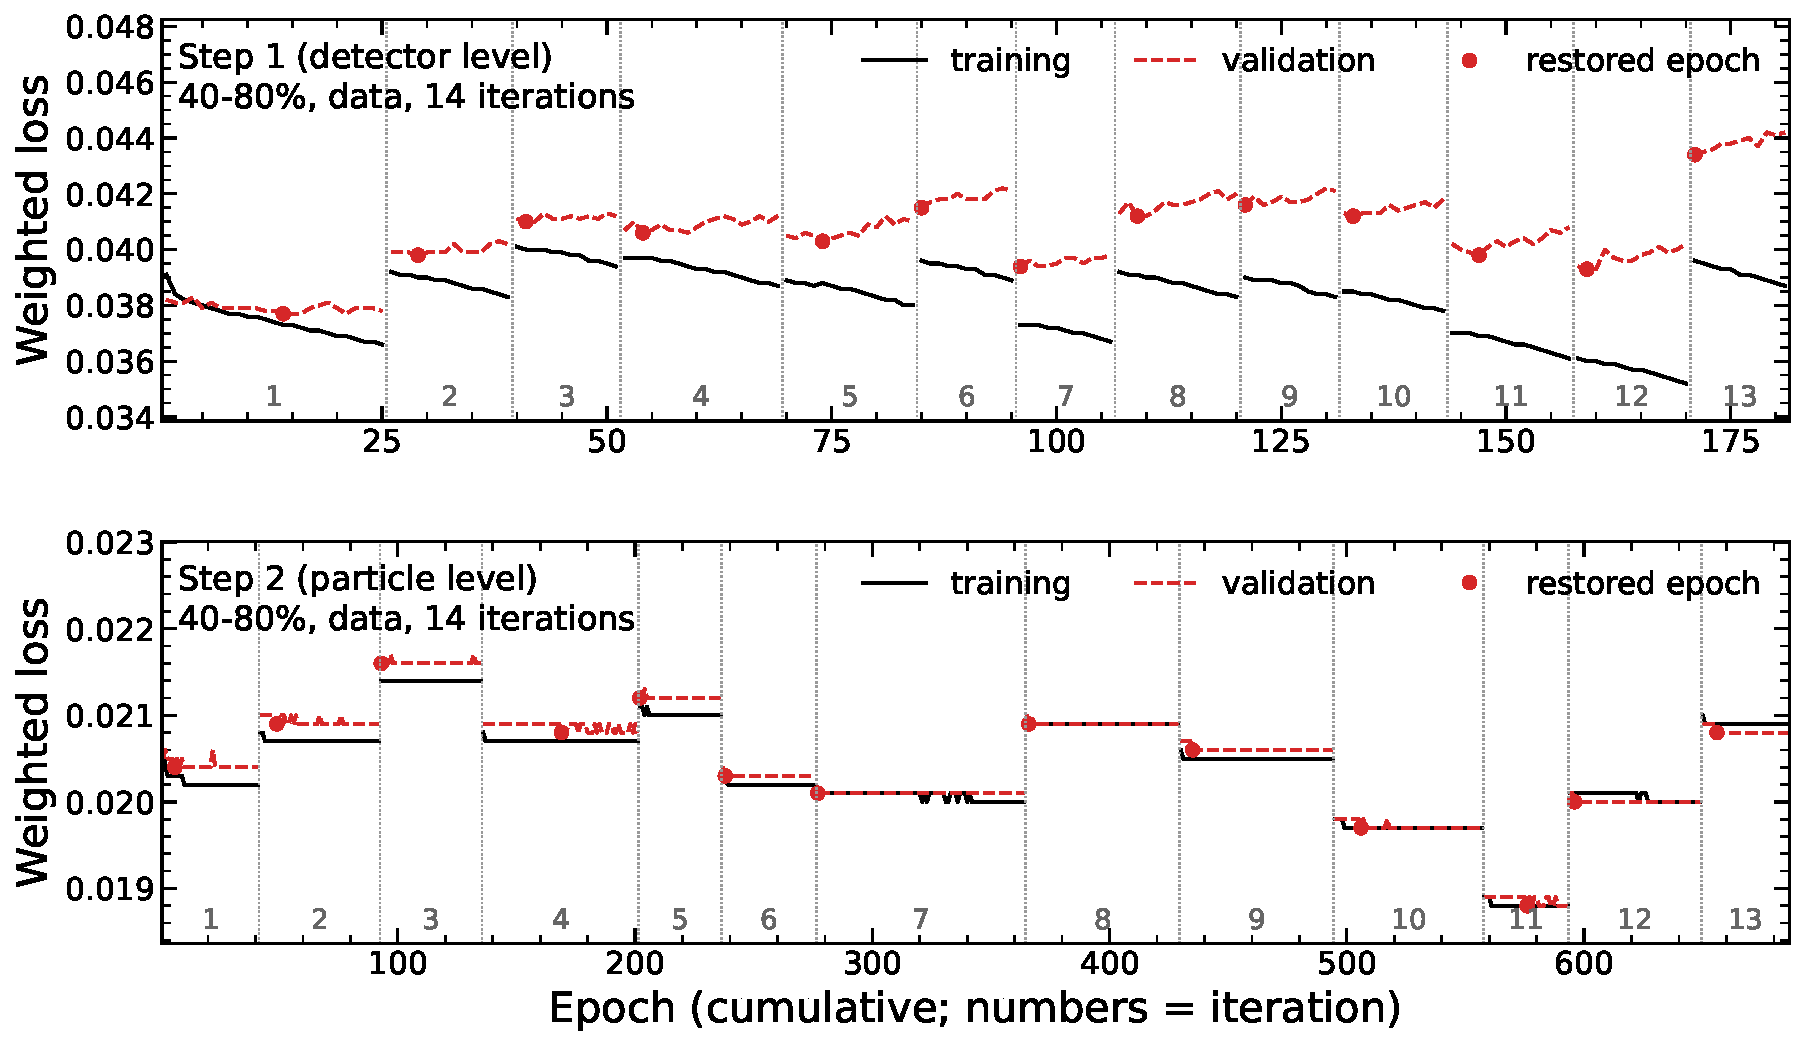
\includegraphics[width=\linewidth]{figures/angularities/AuAu/auau_training_40to80_data.pdf}
	\caption{Evolution of the training (solid black) and validation (dashed red) losses of the MultiFold classifiers over all epochs of all iterations, for a 0-20\% closure run with 10 iterations (left) and a 40-80\% data run with 14 iterations (right), both with the settings of the nominal unfolding. The top (bottom) panels show the step-1 (step-2) classifier, which reweights the embedding to the data at detector level (the prior to the reweighted embedding at particle level). Dotted vertical lines separate the iterations, numbered at the bottom, and red dots mark the epoch with the lowest validation loss, whose network weights are kept and used as the starting point of the next iteration. The loss is the categorical cross-entropy weighted by the per-jet weights.}
	\label{fig:multifoldTraining}
\end{figure}

%
Closure of the MultiFold is a measure of confidence in the algorithm determined by applying a pre-trained MultiFold on a detector level jet sample for which the particle level is known and comparing the two through ratios. 
%
Here, the matched embedding jets of each centrality class (0-20\% and 40-80\%) are randomly split into two independent samples: the detector-level jets of 20\% of them serve as pseudo-data, which are unfolded by a MultiFold trained on the remaining 80\% with the same settings as for the measured data (10 iterations, batch size of 1024), and the unfolded result is compared to the particle-level jets of the pseudo-data sample (pseudo-truth).
%
Since both samples come from the same PYTHIA-6 simulation, this tests the technical closure of the method rather than its dependence on the prior.
%
Proper closure is demonstrated in Fig.\ref{fig:closure} for the obervables studied in these proceedings, with the ratios of distributions being consistent with unity within statistical errors.
\begin{figure}
	\centering
	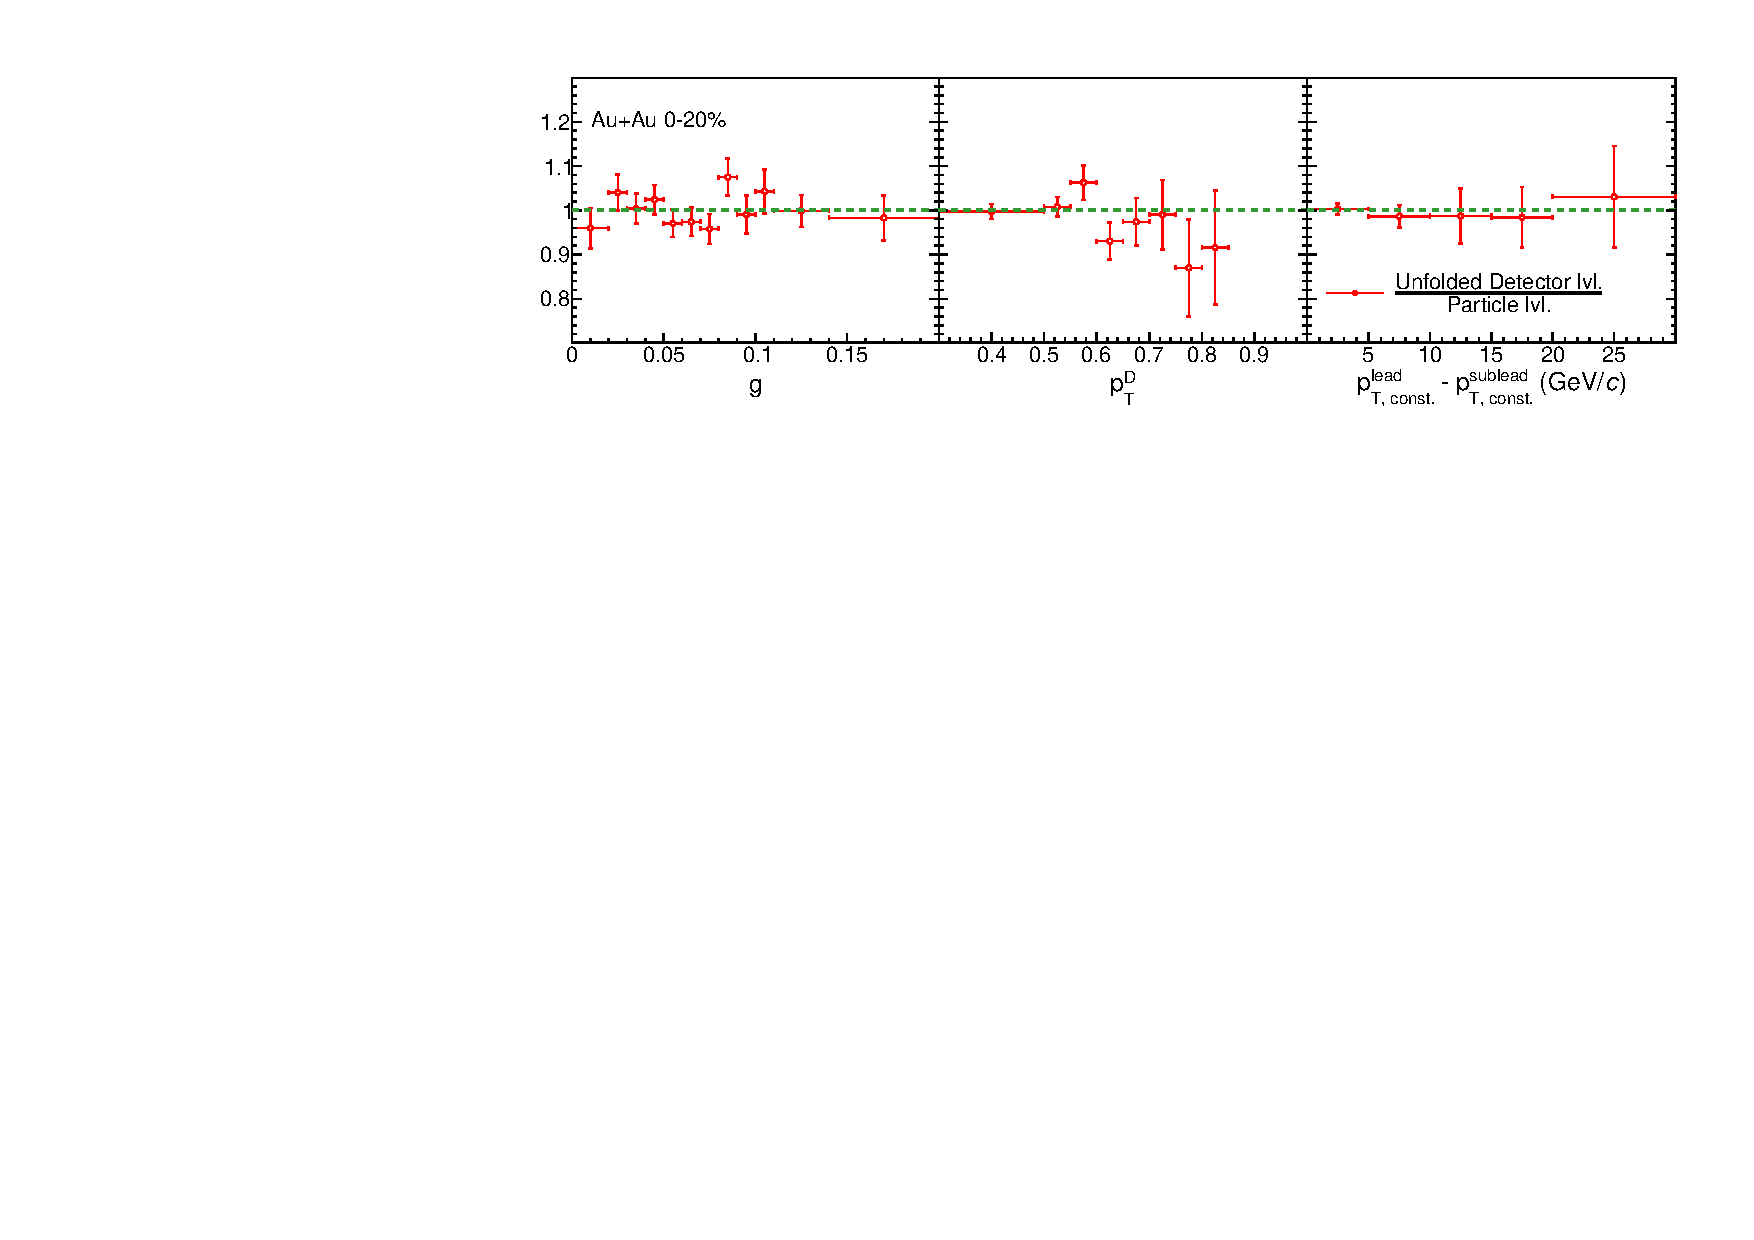
\includegraphics[width=\linewidth]{angularities/AuAu/closure_cent0to20_v3}
	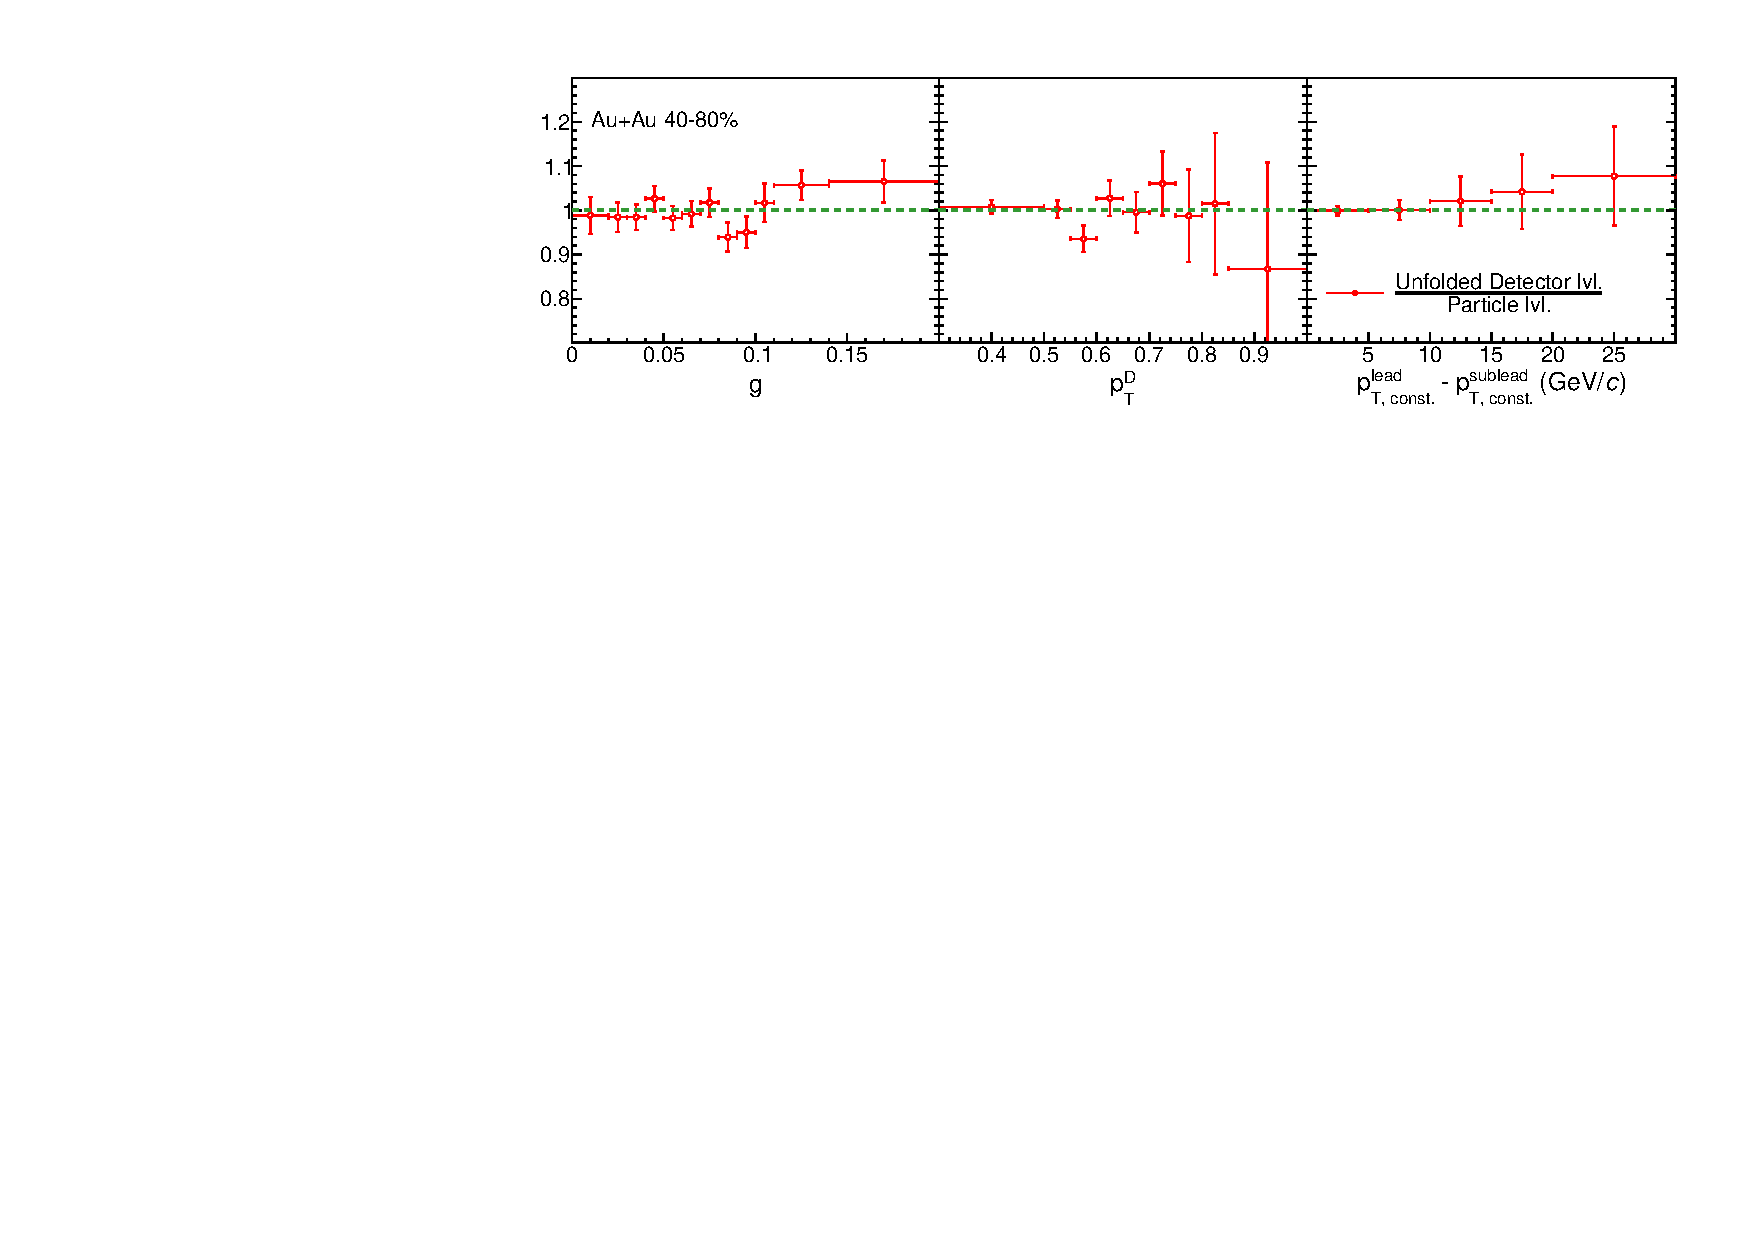
\includegraphics[width=\linewidth]{angularities/AuAu/closure_cent40to80_v3}
	\caption{Closure test for \(g\), \(p_\mathrm{T}^\mathrm{D}\)~and LeSub showing the ratio of distributions calculated using jets from unfolded detector level and particle level events from 0-20\% (top) and 40-80\% (bottom) central Au+Au collisions at \sNN{200}{GeV}.}
	\label{fig:closure}
\end{figure}
This study is the first instance of the MultiFold method being used to deconvolute detector effects from heavy-ion collision events.

\subsection{Systematic Uncertainties}
Three sources of systematic uncertainty are considered, all related to the unfolding.
%
The regularization of MultiFold is varied by changing the number of iterations from 10 to 14, and the relative difference between the two unfolded distributions is taken as an uncertainty.
%
Any residual non-closure from MultiFold, the deviation from unity of the closure ratios in Fig.~\ref{fig:closure} evaluated in each \(p_\mathrm{T, jet}\) bin, was also included as an uncertainty.
%
A prior variation uncertainty was added from previous calculations using STAR $\sqrt{s} = 200$ GeV p+p collision data.
%
In each bin, the largest of the three relative deviations is taken as the total systematic uncertainty.
%
The breakdown of the systematic uncertainty by source is shown in Fig.~\ref{fig:AuAuSys}, for both centrality classes, both \(p_\mathrm{T, jet}\) bins and the ratio of central to peripheral distributions.
%
The total is typically 5-20\%, and grows in the sparsely populated tails of the distributions, up to about 90\% at large \(g\) in central collisions, where the change of the number of iterations dominates.
%
Elsewhere the total is set by either the prior or the iteration variation, while the non-closure is the largest source only in a few bins.
%
The statistical uncertainties are below about 10\%, except in the highest LeSub bin at \ptRange{jet}{15}{20}, where they reach about 30\%.
%
For the ratio of central to peripheral distributions, the total uncertainties of the two centrality classes are added in quadrature, i.e. they are assumed to be uncorrelated. This is a conservative choice, since the unfolding-related variations are expected to shift both centrality classes in the same direction.
%
Detector-level sources such as the tracking efficiency (Sect.~\ref{sec:TrackTowerSel}) and the tower energy scale were not evaluated in this exploratory analysis.
\begin{sidewaysfigure}
	\centering
	\begin{tabularx}{\textwidth}{XXX}
		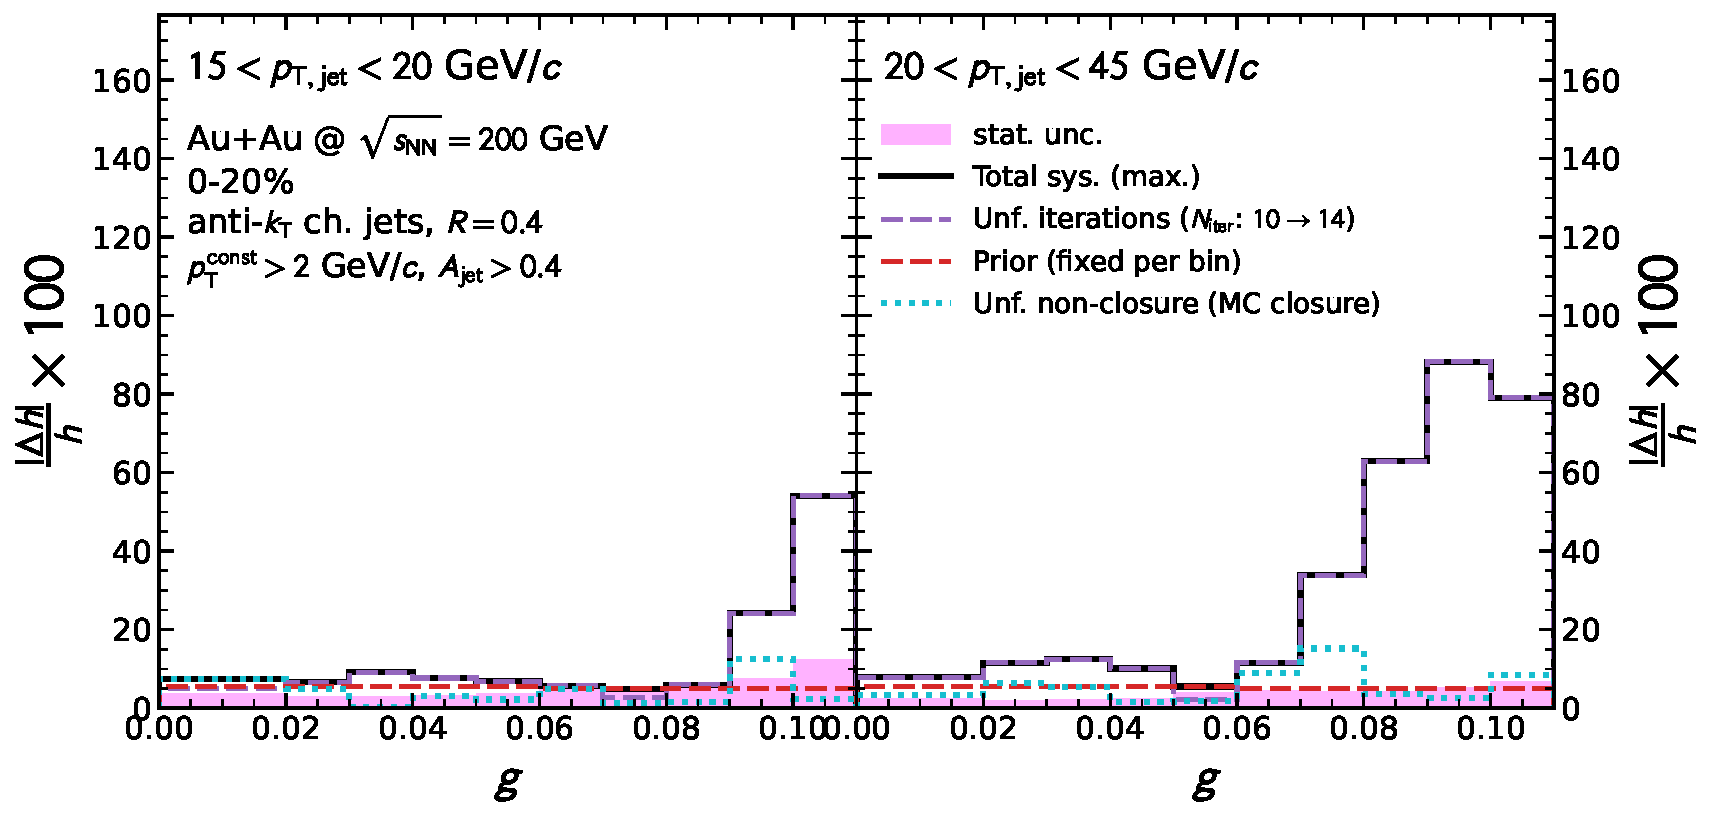
\includegraphics[width=\linewidth]{angularities/AuAu/auau_sys_Girth_cent0to20.pdf} &
		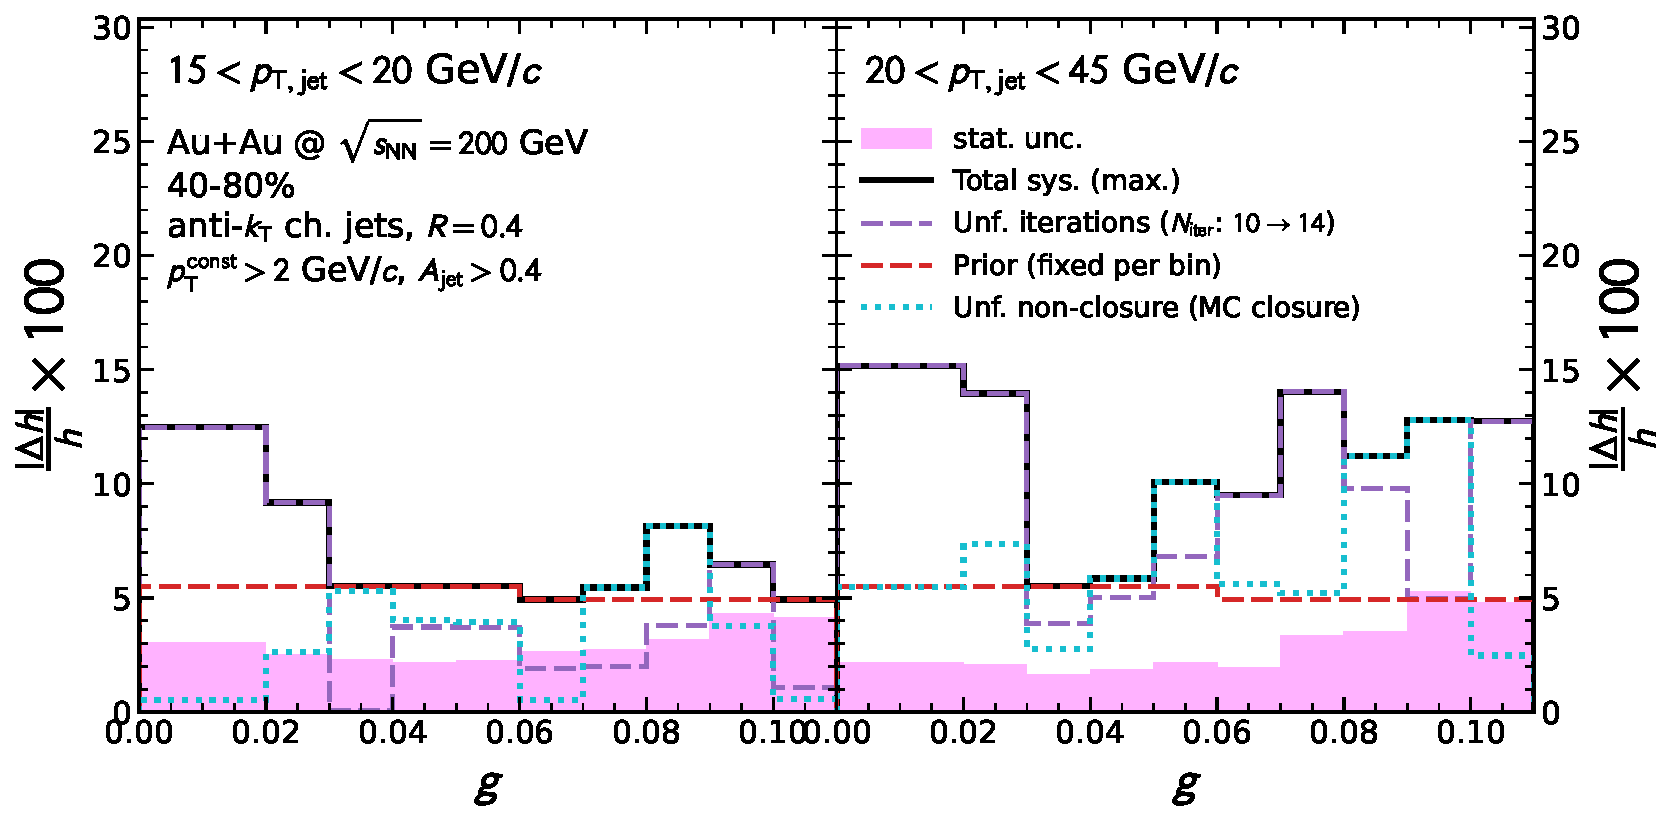
\includegraphics[width=\linewidth]{angularities/AuAu/auau_sys_Girth_cent40to80.pdf} &
		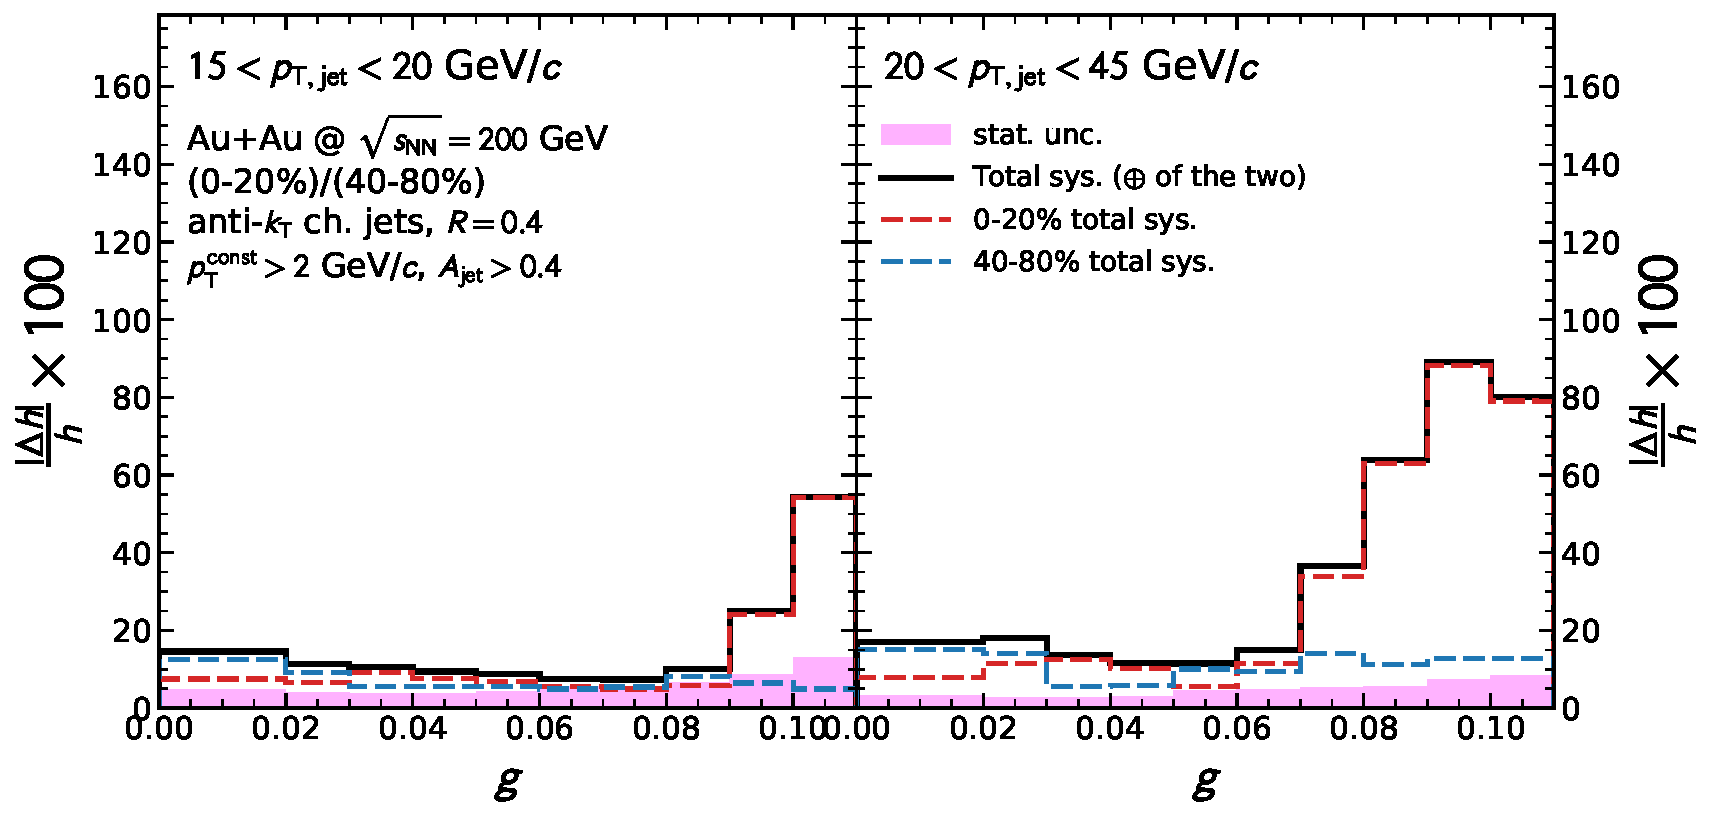
\includegraphics[width=\linewidth]{angularities/AuAu/auau_sys_Girth_ratio.pdf} \\
		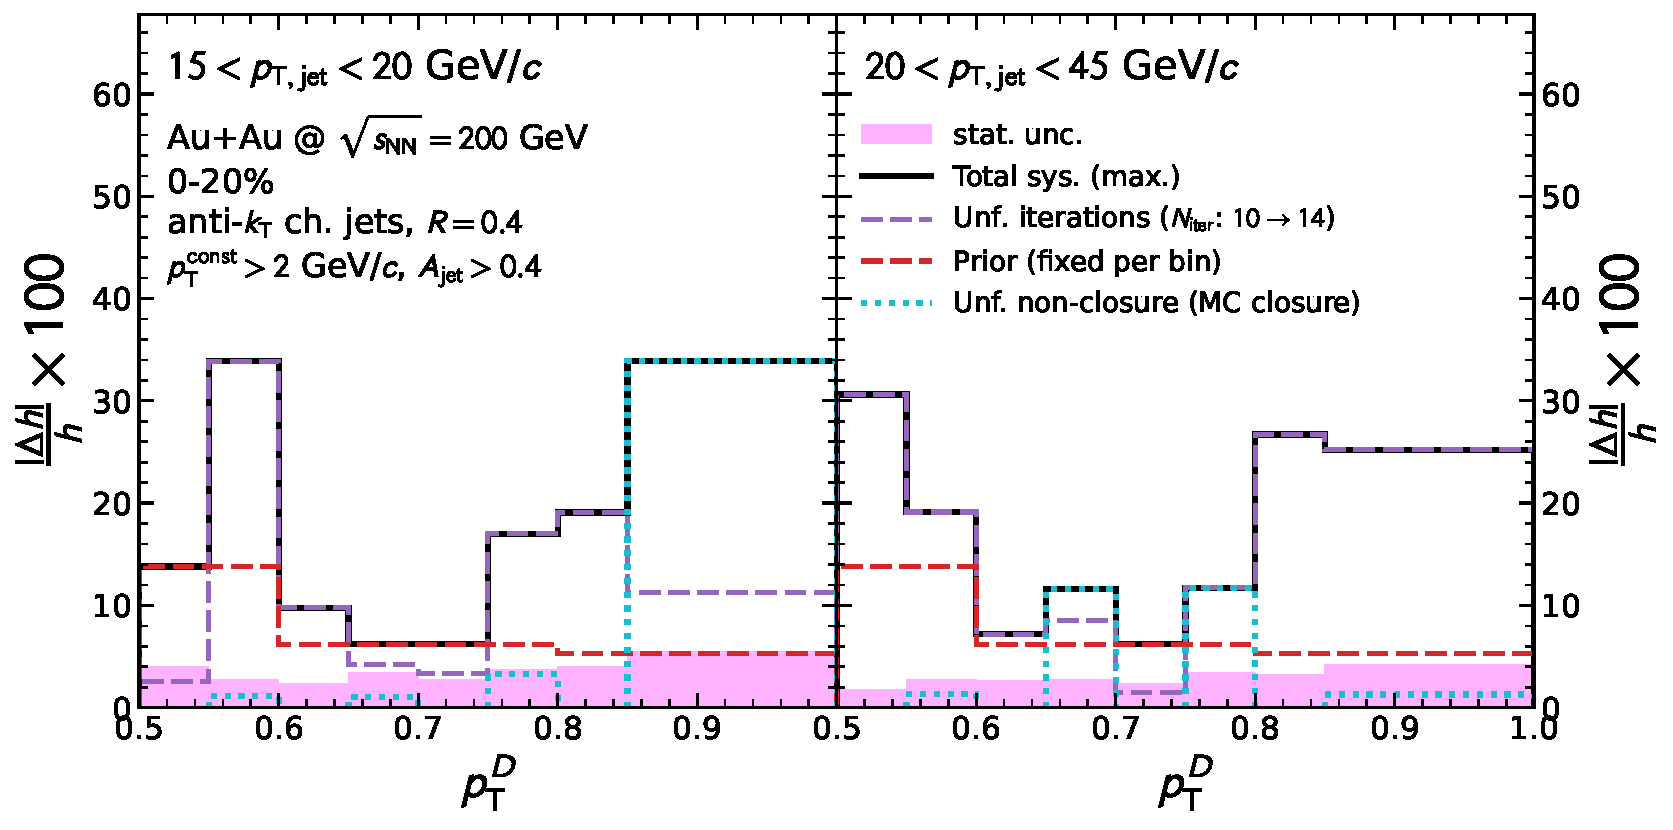
\includegraphics[width=\linewidth]{angularities/AuAu/auau_sys_PtD_cent0to20.pdf} &
		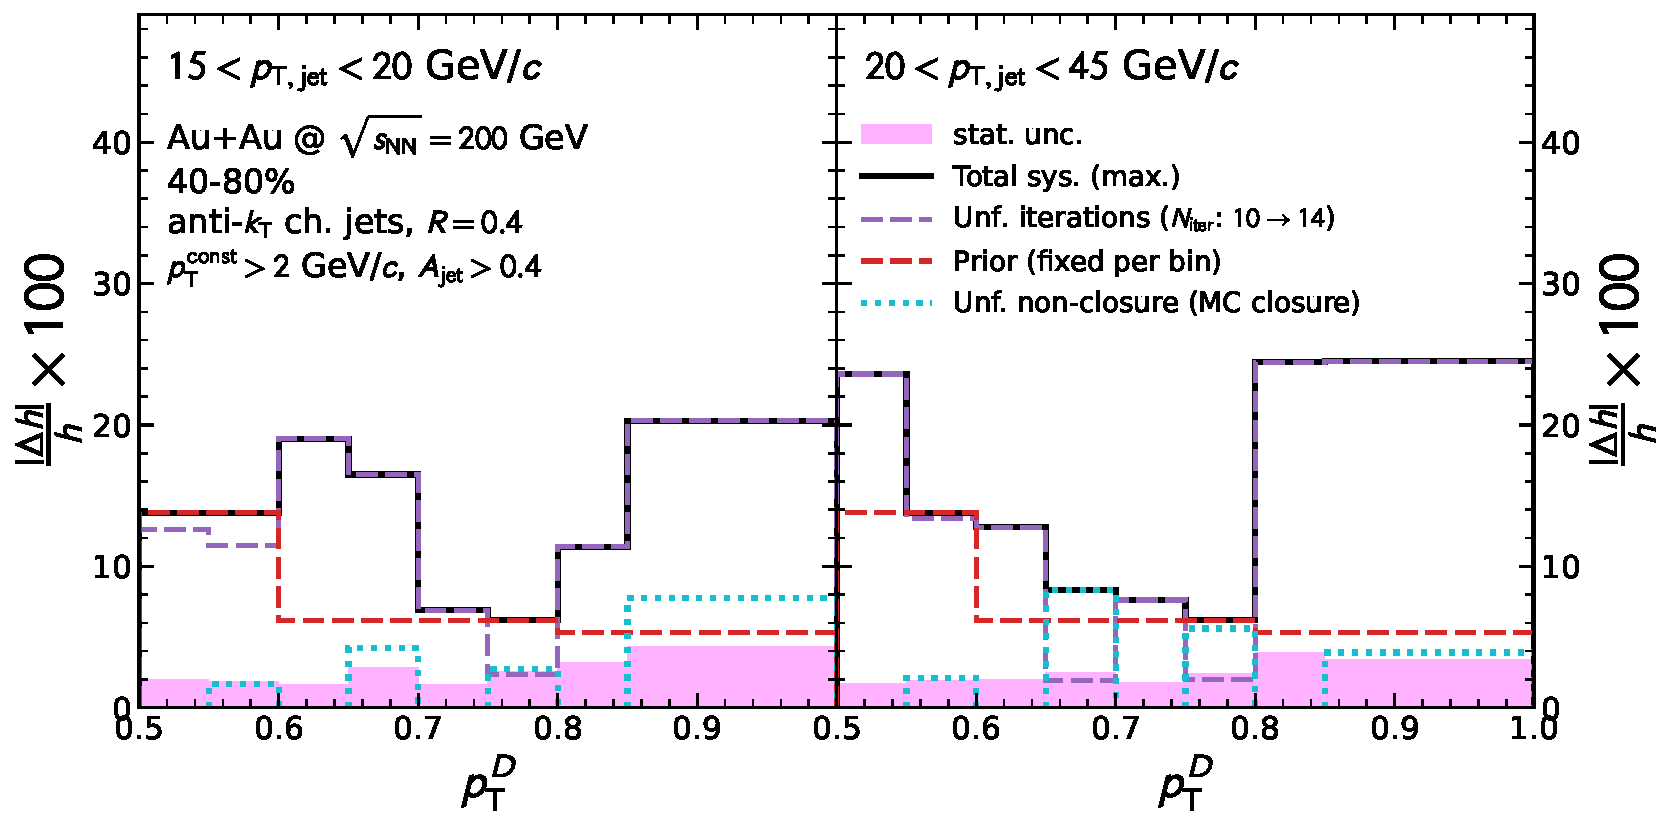
\includegraphics[width=\linewidth]{angularities/AuAu/auau_sys_PtD_cent40to80.pdf} &
		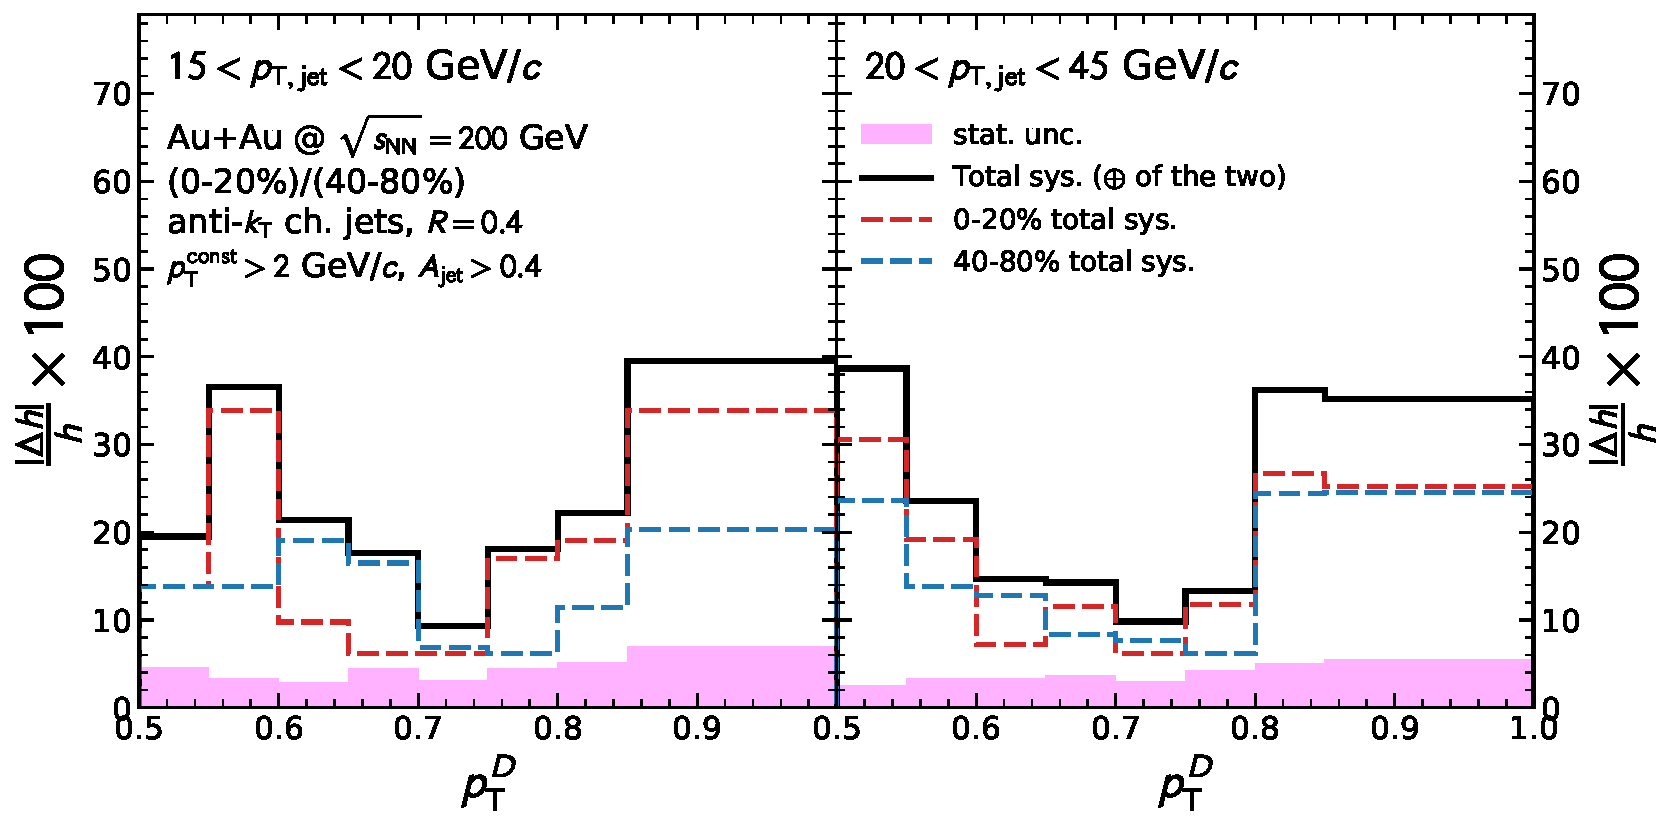
\includegraphics[width=\linewidth]{angularities/AuAu/auau_sys_PtD_ratio.pdf} \\
		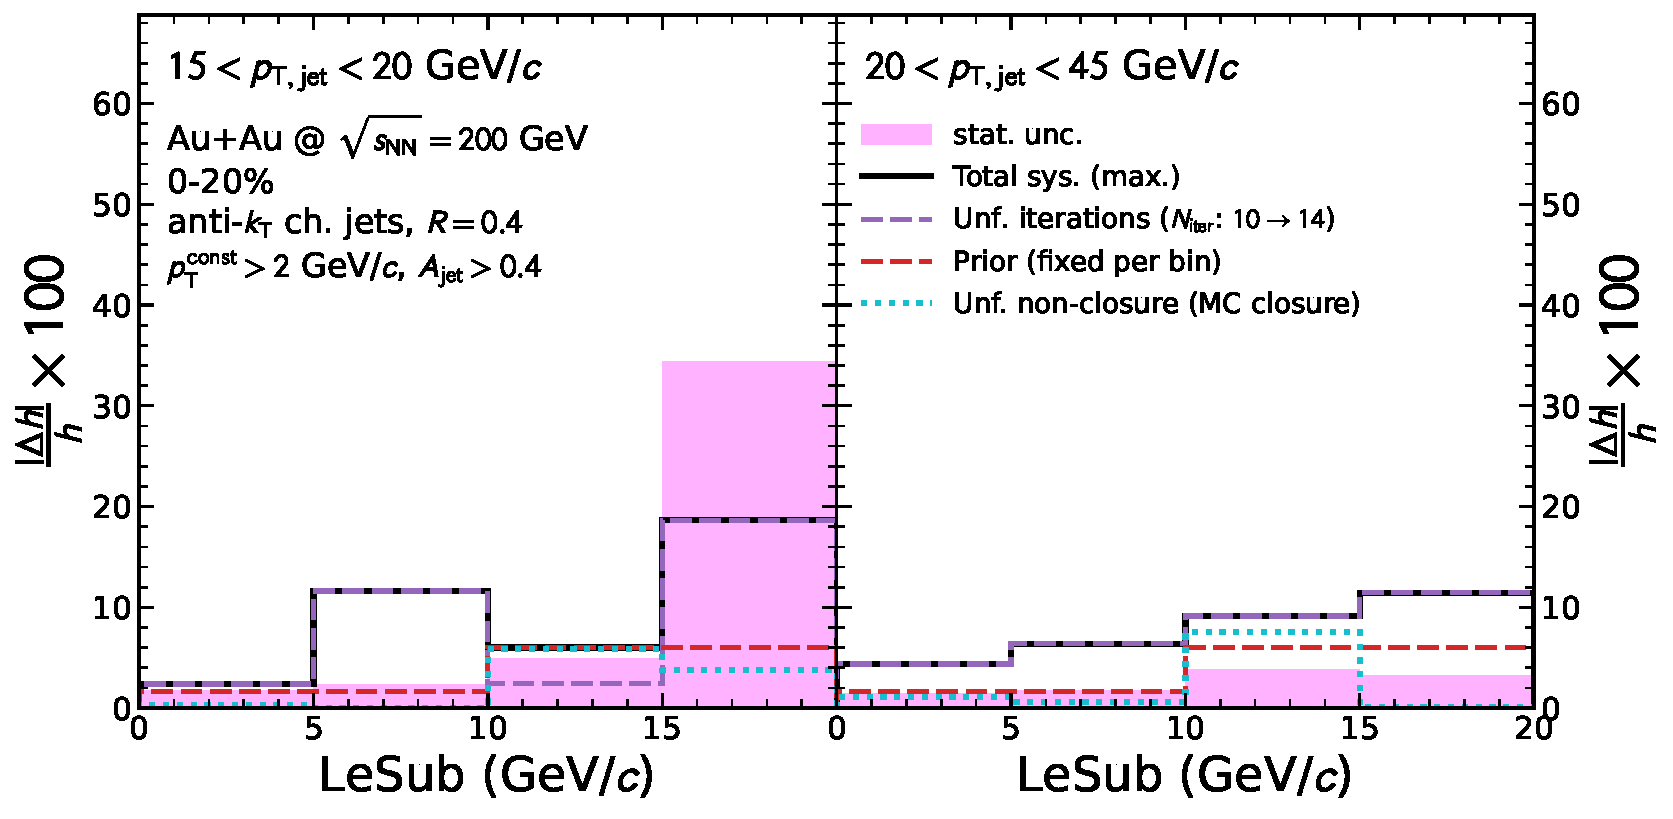
\includegraphics[width=\linewidth]{angularities/AuAu/auau_sys_LeSub_cent0to20.pdf} &
		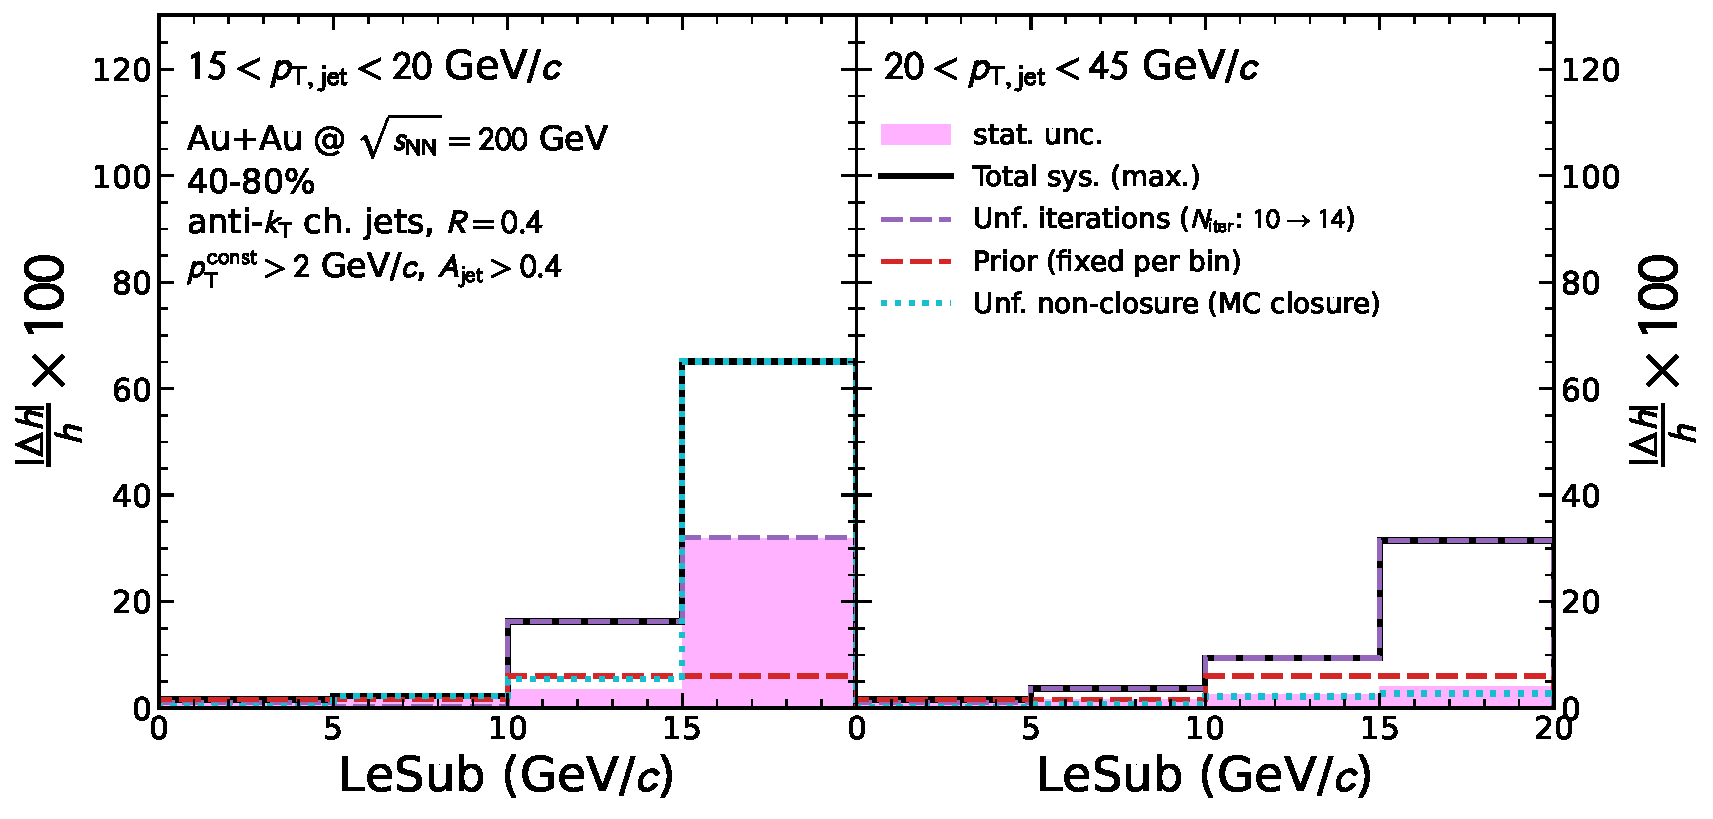
\includegraphics[width=\linewidth]{angularities/AuAu/auau_sys_LeSub_cent40to80.pdf} &
		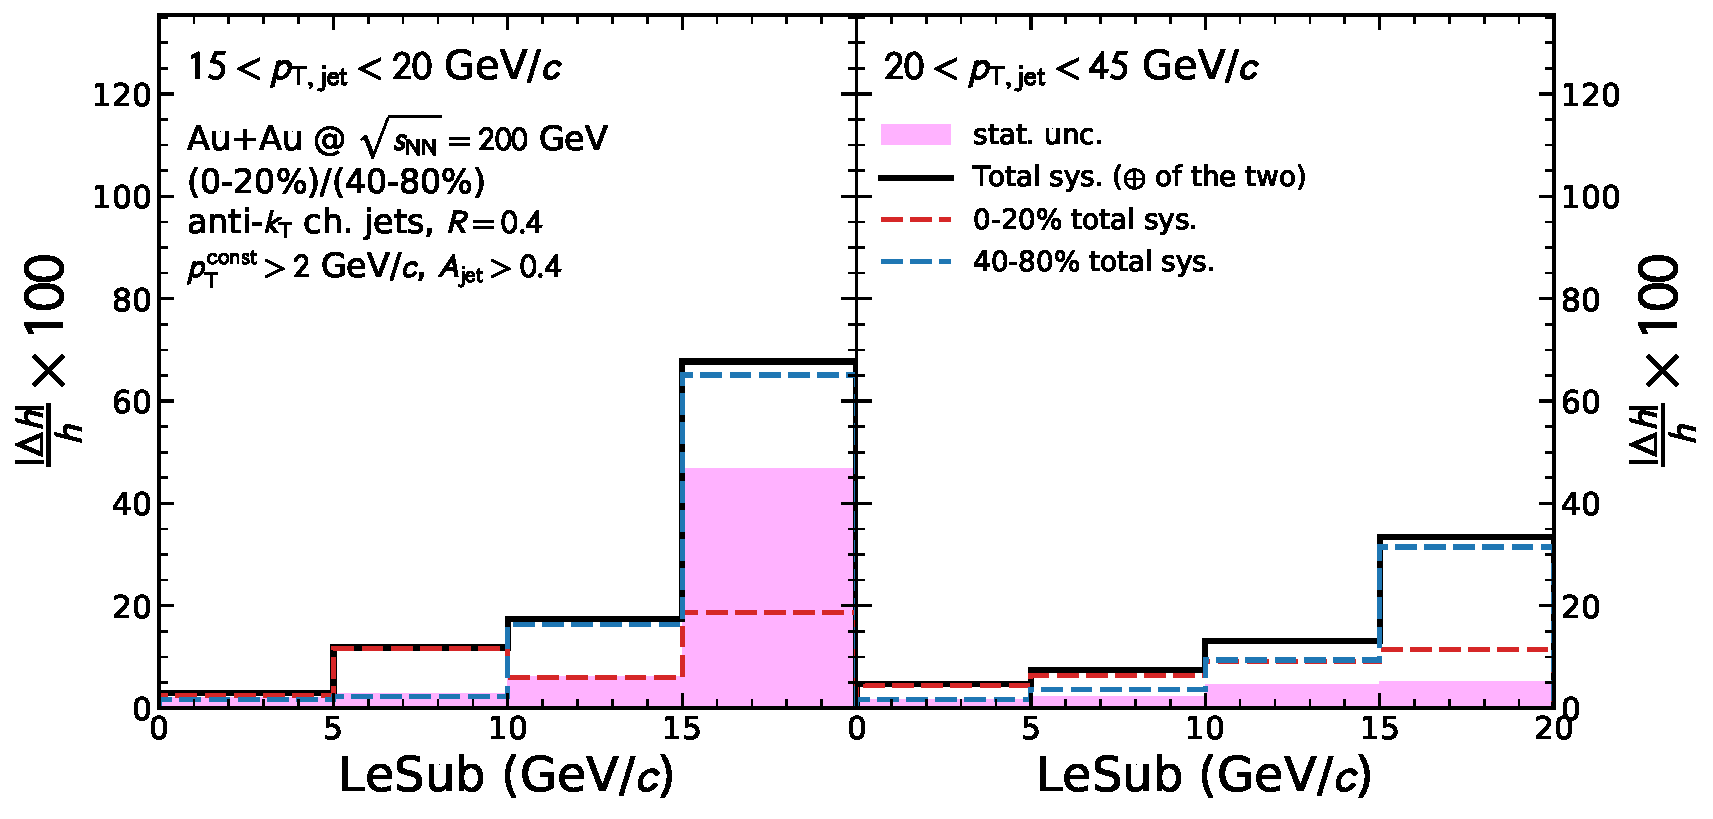
\includegraphics[width=\linewidth]{angularities/AuAu/auau_sys_LeSub_ratio.pdf} \\
\end{tabularx}
\caption{Relative systematic uncertainties of the unfolded \(g\) (top), \(p_\mathrm{T}^\mathrm{D}\) (middle) and LeSub (bottom) distributions for 0-20\% (left) and 40-80\% (middle) central Au+Au collisions at \sNN{200}{GeV}, and of their central over peripheral ratio (right). Each plot shows jets with \ptRange{jet}{15}{20} (left panel) and \ptRange{jet}{20}{45} (right panel). The magenta band is the statistical uncertainty. In the left and middle columns, the dashed purple, dashed red and dotted cyan lines are the uncertainties from the number of MultiFold iterations, the prior and the MultiFold non-closure respectively, and the solid black line is the total, their maximum in each bin. In the right column, the dashed red (blue) line is the total uncertainty for 0-20\% (40-80\%) collisions, and the solid black line is their sum in quadrature.}
\label{fig:AuAuSys}
\end{sidewaysfigure}

\subsection{Result and Discussion}
\begin{figure}
	\centering
	\begin{tabularx}{\textwidth}{XX}
		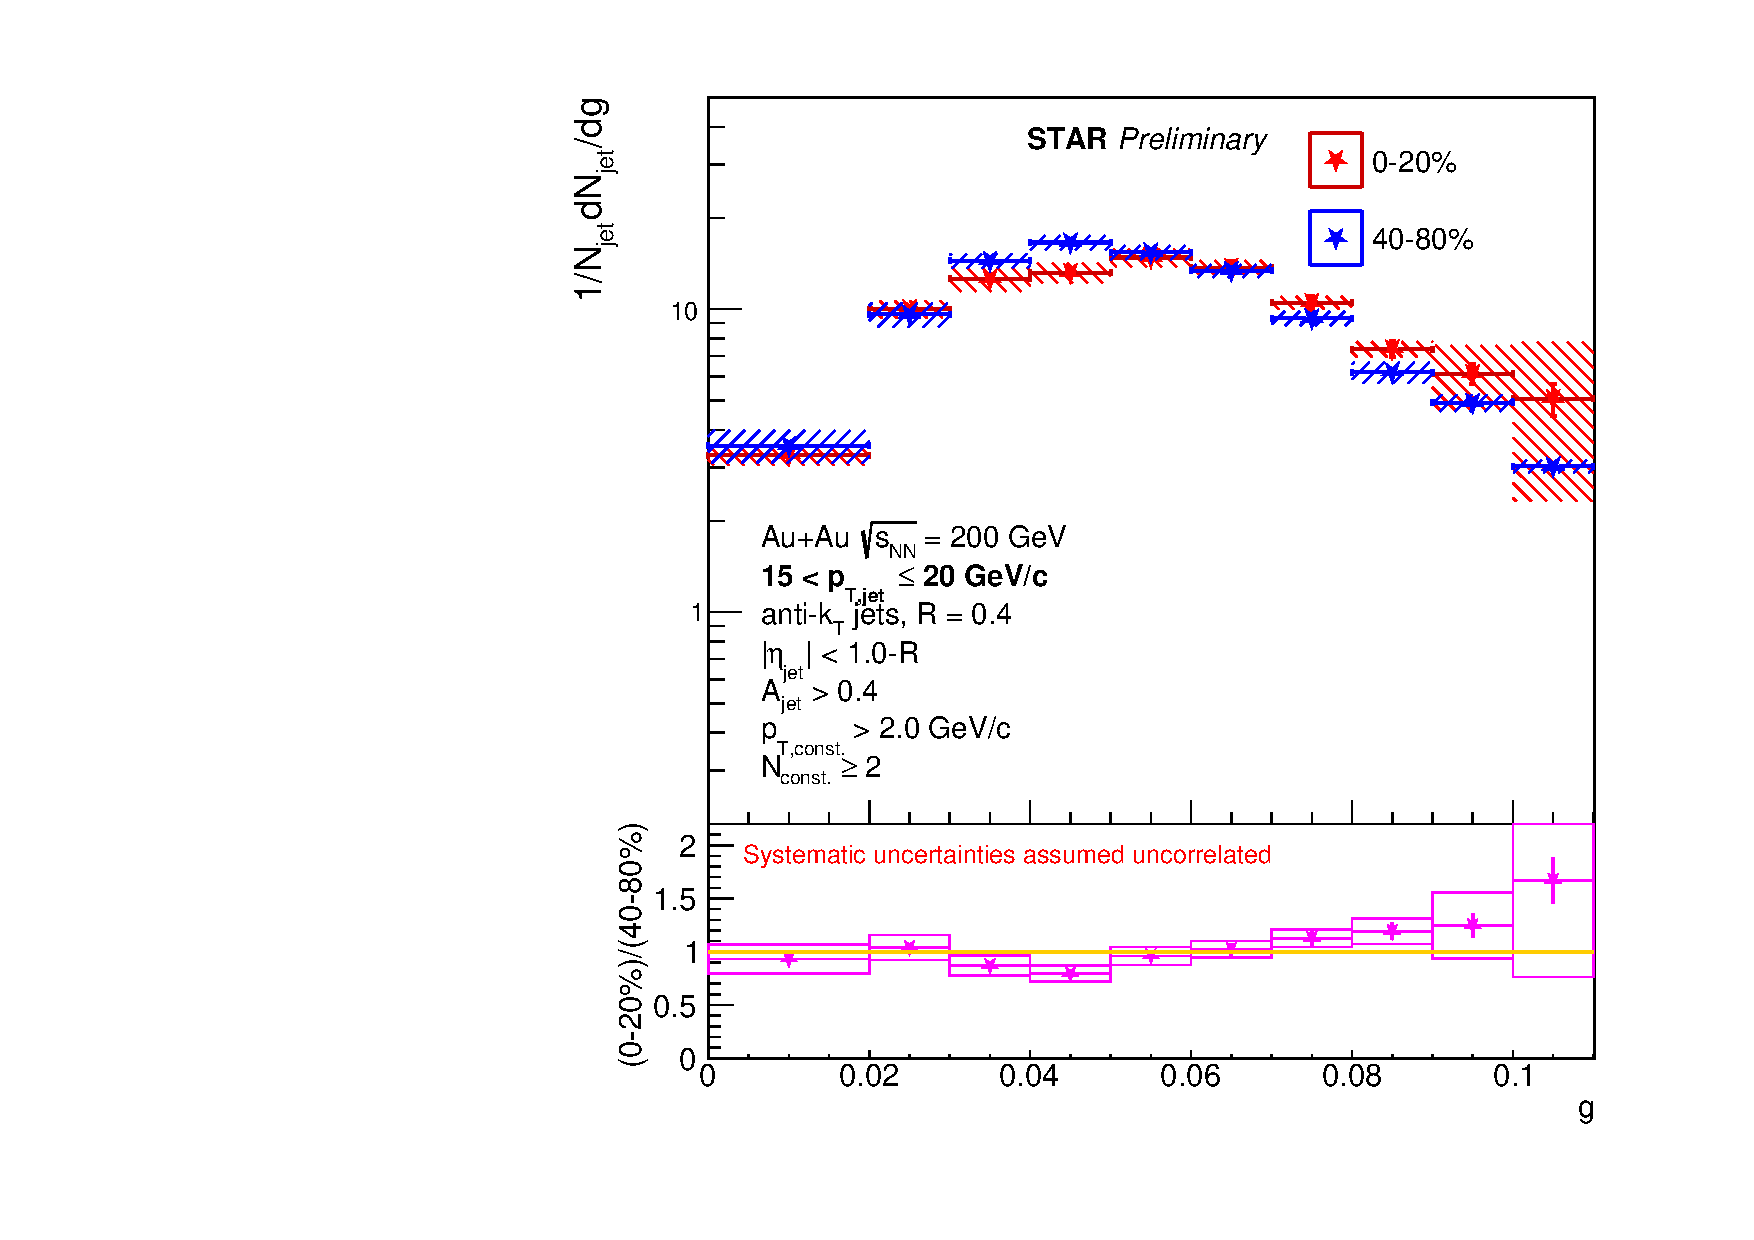
\includegraphics[width=\linewidth]{angularities/AuAu/finalPlots_noPP_Girth_0_v3_warn.pdf} &
		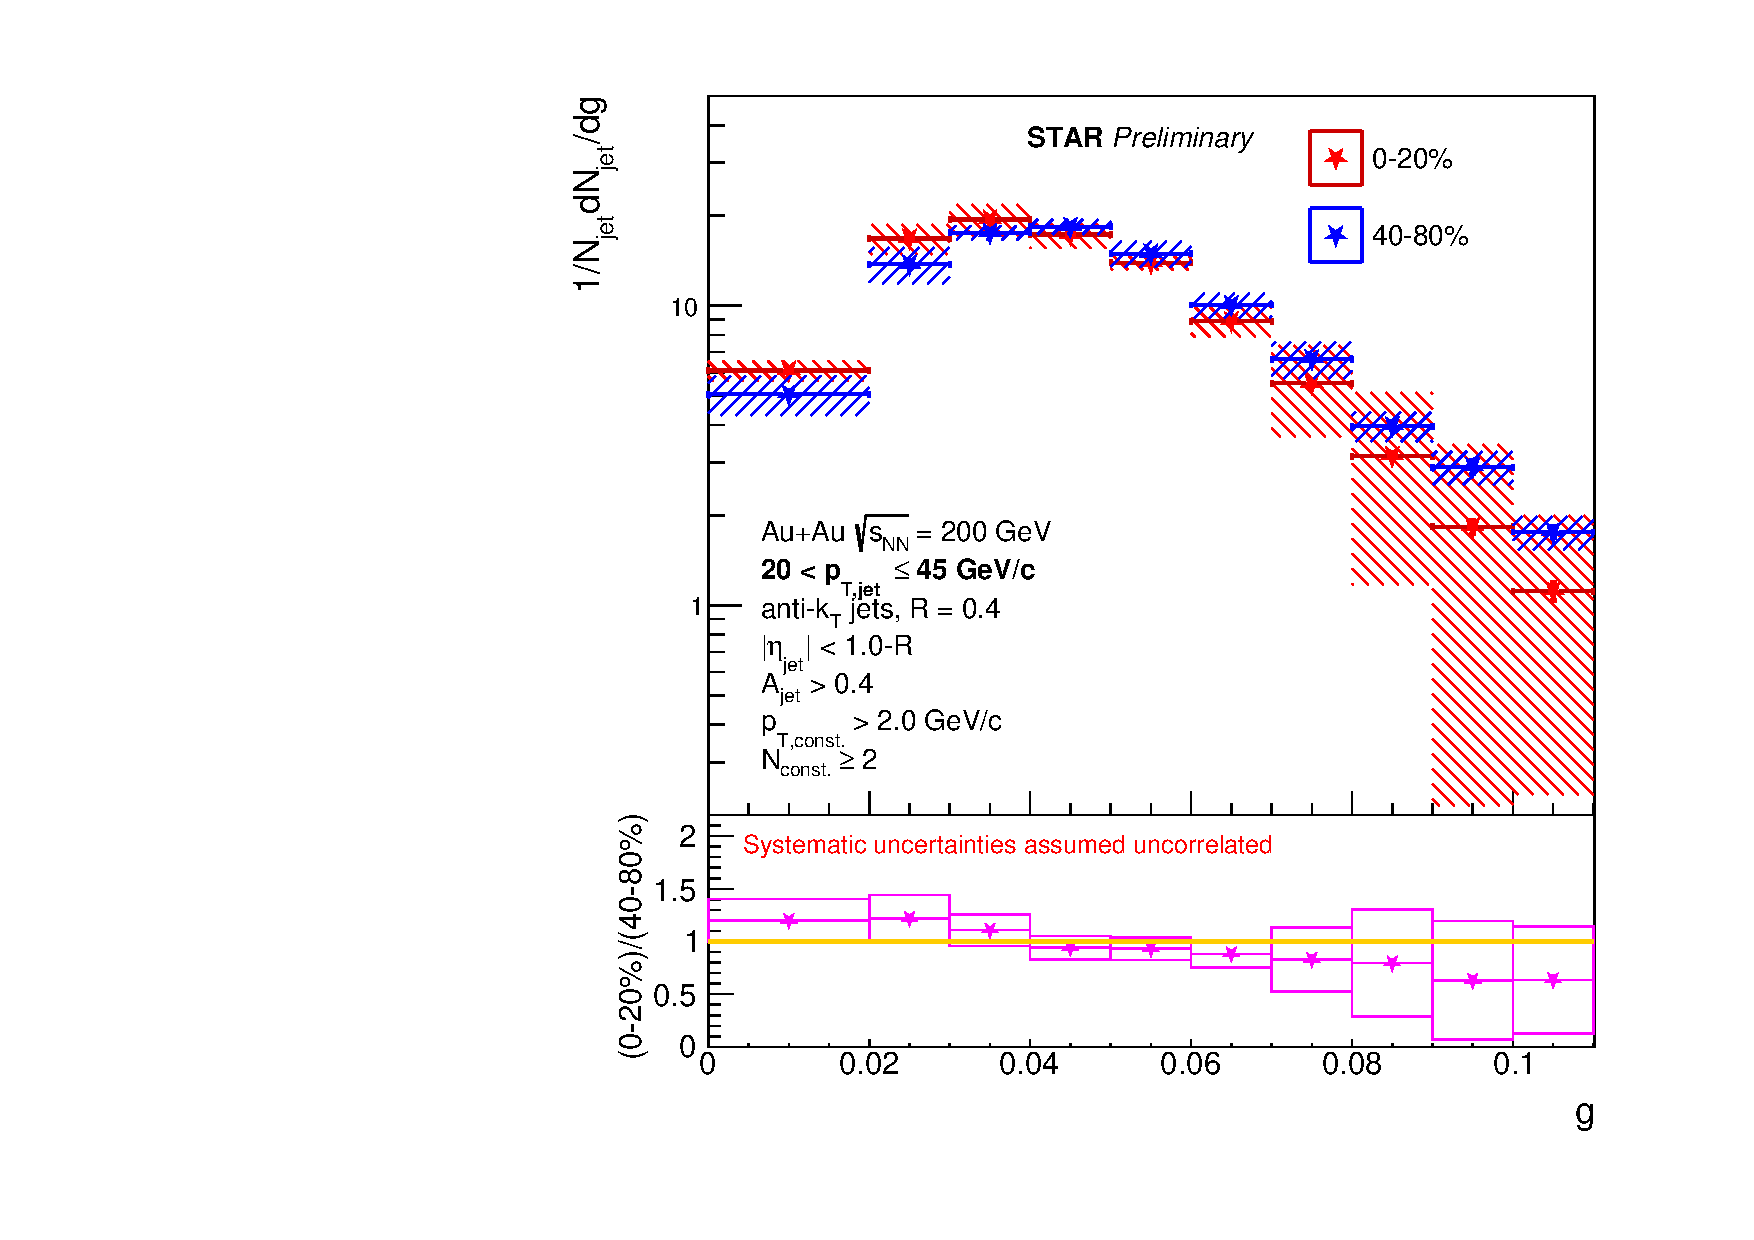
\includegraphics[width=\linewidth]{angularities/AuAu/finalPlots_noPP_Girth_1_v3_warn.pdf} \\
		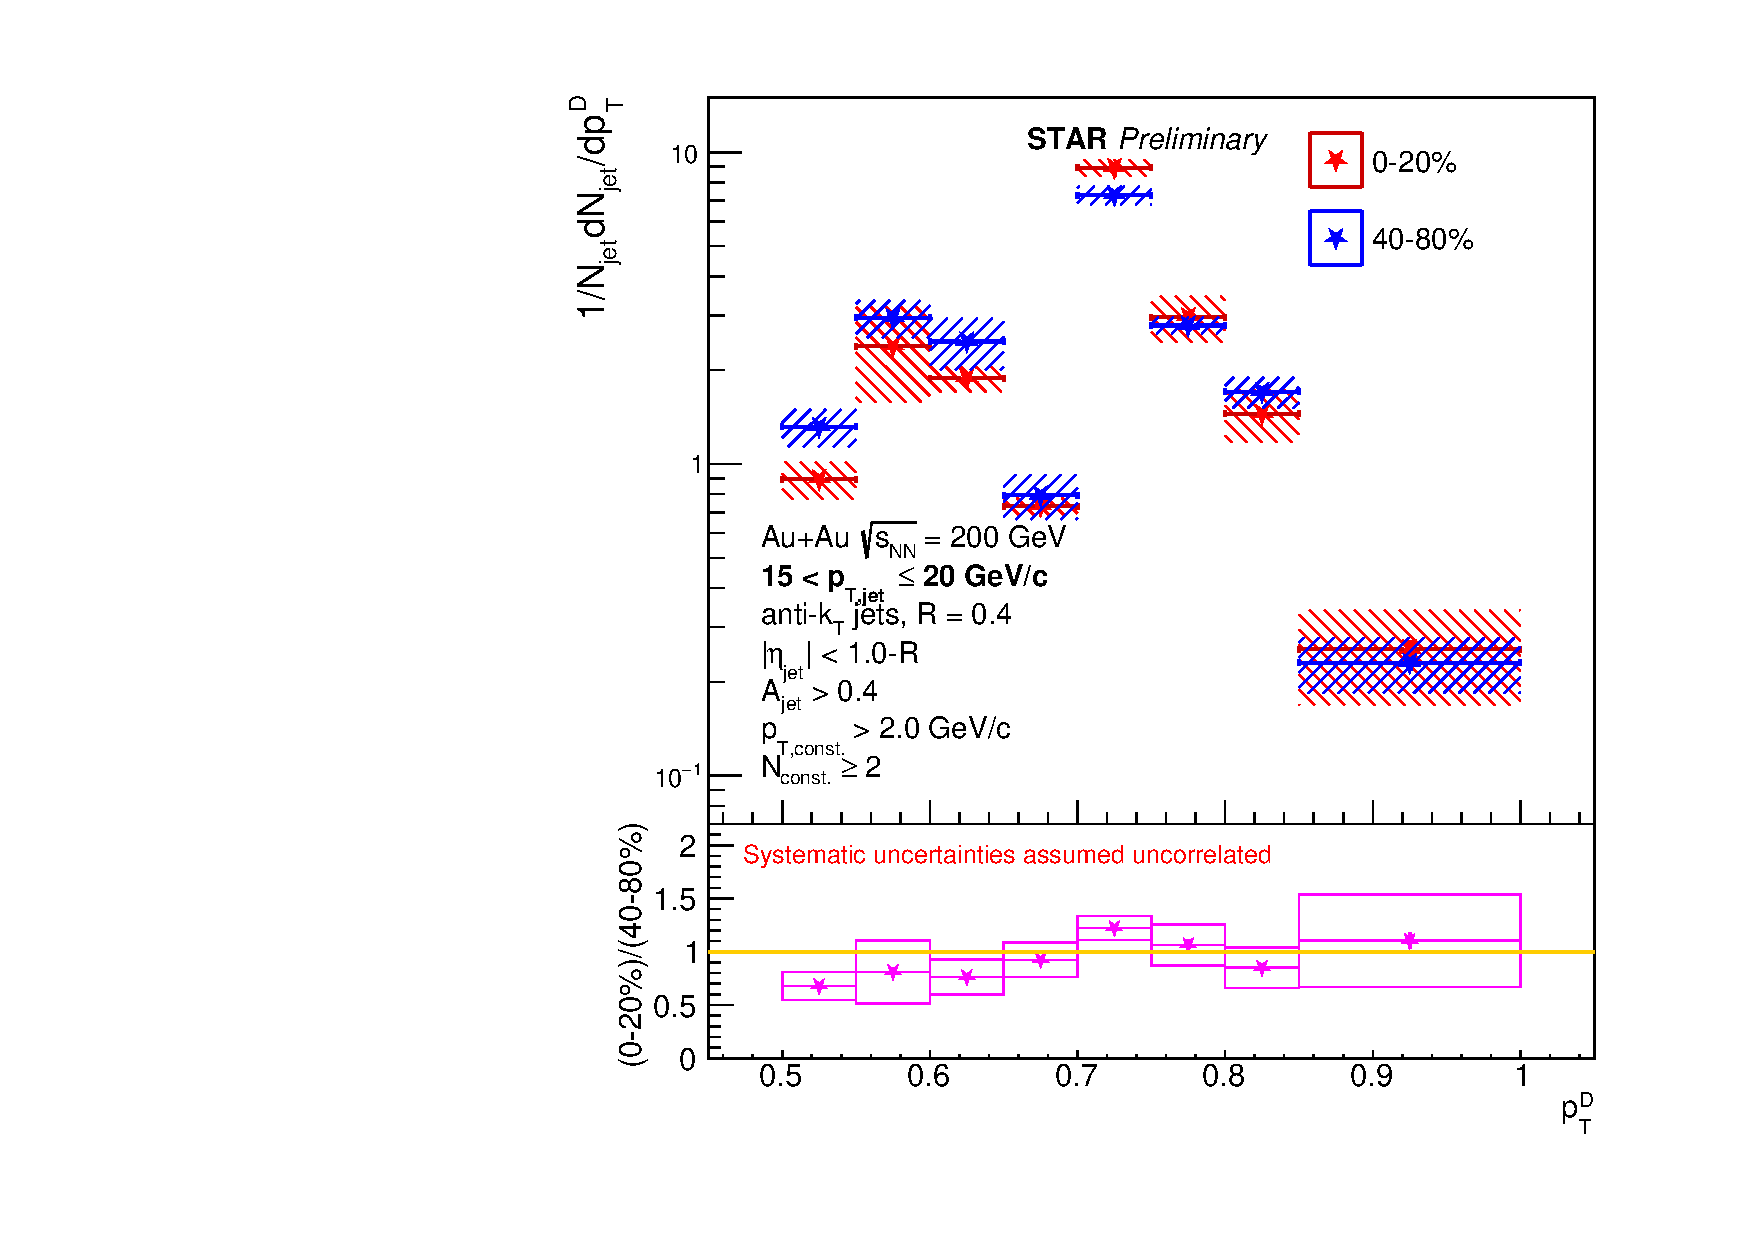
\includegraphics[width=\linewidth]{angularities/AuAu/finalPlots_noPP_PtD_0_v3_warn.pdf} &
		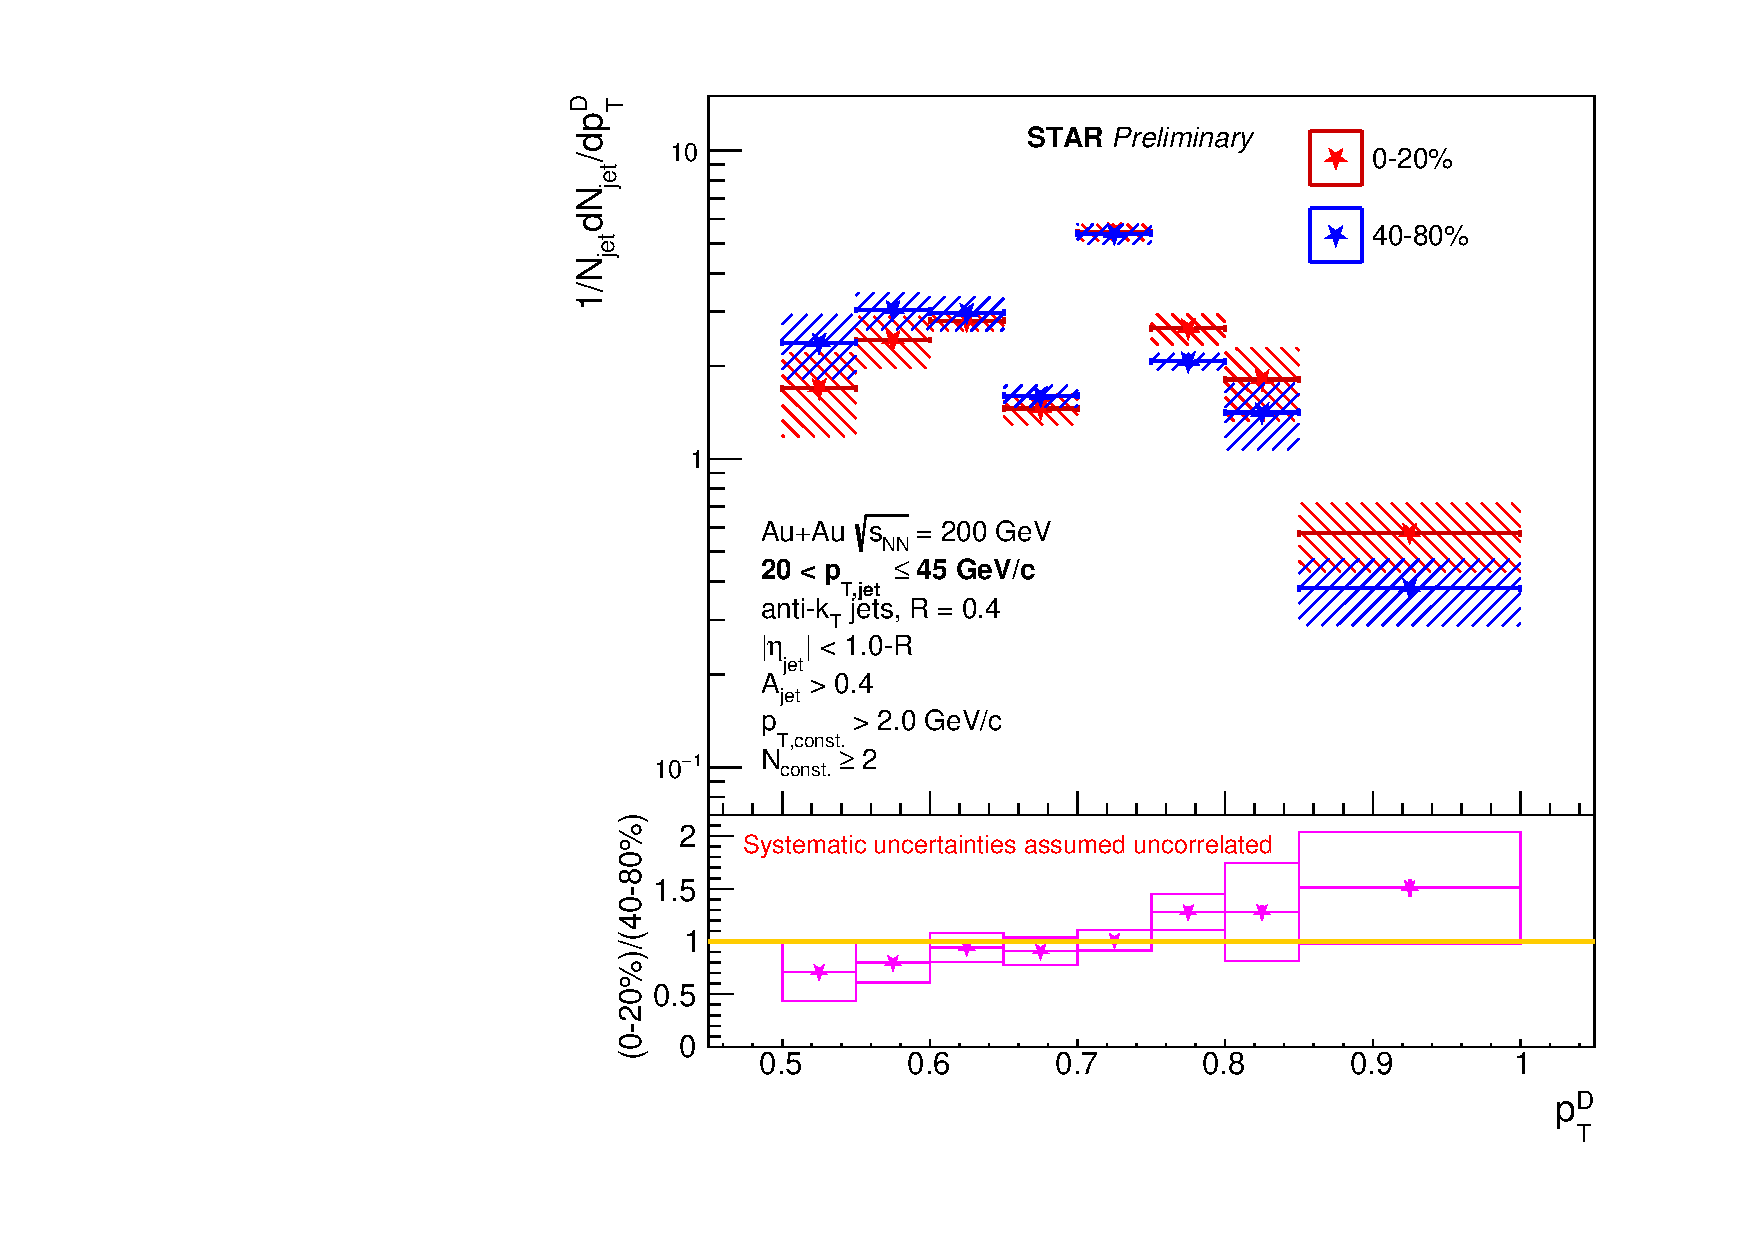
\includegraphics[width=\linewidth]{angularities/AuAu/finalPlots_noPP_PtD_1_v3_warn.pdf} \\
		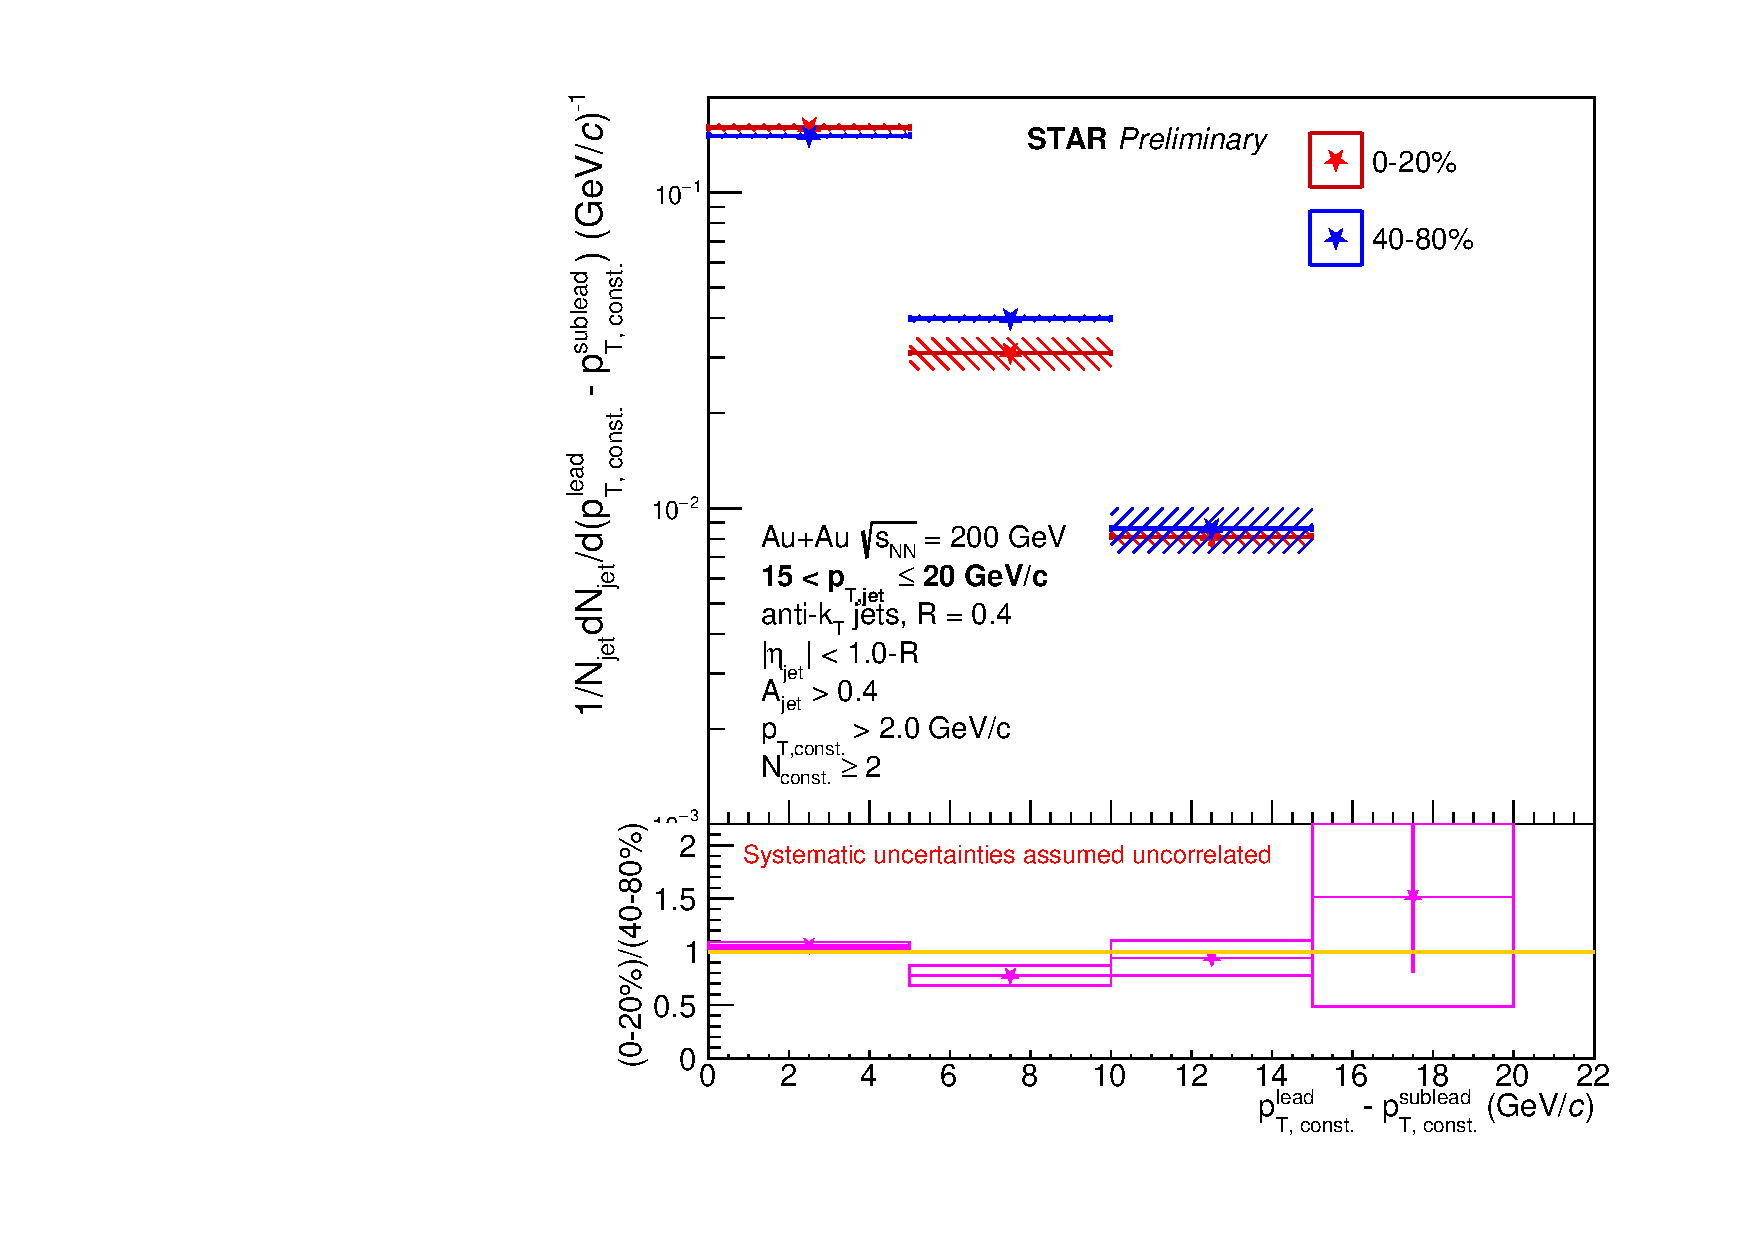
\includegraphics[width=\linewidth]{angularities/AuAu/finalPlots_noPP_LeSub_0_v3_warn.pdf} &
		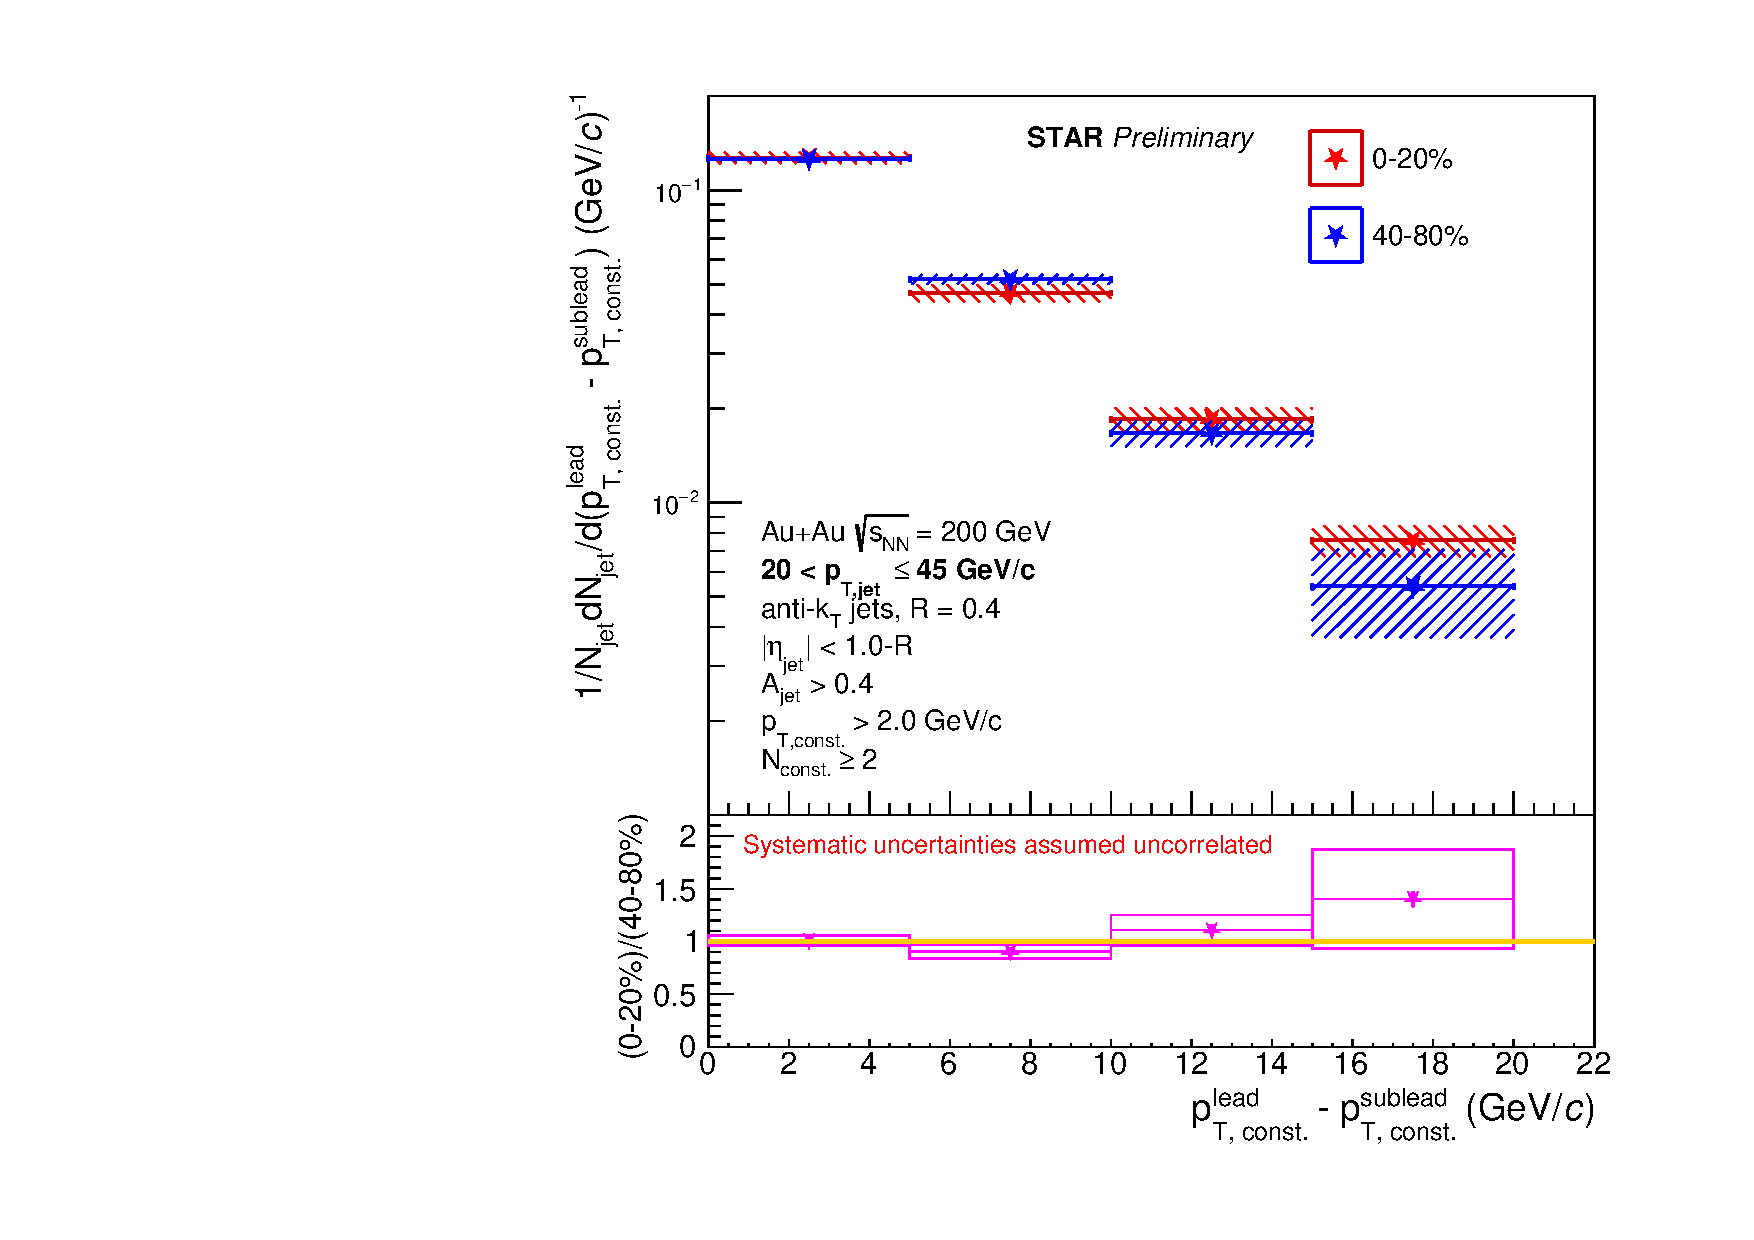
\includegraphics[width=\linewidth]{angularities/AuAu/finalPlots_noPP_LeSub_1_v3_warn.pdf} \\
	\end{tabularx}
	\caption{Unfolded, normalized distributions of \(g = \lambda_1^1\) (top), \(p_\mathrm{T}^\mathrm{D}\) (middle) and LeSub (bottom) for jets with \ptRange{jet}{15}{20} (left) and \ptRange{jet}{20}{45} (right) from central (0-20\%, red stars) and peripheral (40-80\%, blue stars) Au+Au collisions at \sNN{200}{GeV}. Systematic uncertainties are shown as hatched boxes. Central over peripheral ratios (magenta stars) are in the lower panels with their systematic uncertainties represented as magenta boxes. Systematic uncertainties are assumed to be uncorrelated between the centrality ranges. }
	\label{fig:AuAu_JSO}	
\end{figure}
Fully corrected measurements of \(g\), \(p_\mathrm{T}^\mathrm{D}\)~and LeSub distributions calculated from jets with \ptRange{jet}{15}{20} and \ptRange{jet}{20}{45} from events within centrality ranges of 0-20\% (central) and 40-80\% (peripheral), and \(R_{CP}\) ratio comparisons between distributions from  central and peripheral events calculated according to Eq.~\ref{eq:IntroRCP} are shown in Fig.~\ref{fig:AuAu_JSO}. 
%
The \(p_\mathrm{T}^\mathrm{D}\)~distribution shows a discontinuity at 0.7 due to the strong dependence on number of constituents in jet. 
%
Results are consistent between central and peripheral collisions within conservative systematic uncertainties. 
%
This can be attributed to the assumption of uncorrelated systematic uncertainties, and a bias in the analysis towards hard-fragmented jets due to the selection of events and constituents for jet clustering. 
%
Harder-fragmented jets, on average are narrower and have lower interaction time with QGP, which could make any relative modification in central events compared to the peripheral ones lower than what would be potentially observed in an inclusive jet analysis. 
%
This is the first heavy-ion analysis to use unbinned unfolding of detector effects, hence there is room for improvement in application of the technique, which will be explored in the next section.

\section{Inclusive and groomed angularities of \(p + p\) jets}
The last section showed that valuable information about jet substructure is lost by over-subtracting background with a naive tool like a hard-core constituent cut.
%
Therefore, a more sophisticated method of isolating perturbative and non-perturbative effects must be used.
%
One such method used in this analysis is the SoftDrop~\cite{SoftDrop_Larkoski_2014} grooming.
%
However, before  the last section's analysis is repeated with groomed jets, the unbinned unfolding techniques must be studied, understood and developed for RHIC data in a simpler system.
%
Thus the \(p+p\) angularities study presented here serves a three-fold purpose.
%
First, it provides a baseline for future inclusive and groomed angularity studies in heavy-ion collisions at \sNN{200}{GeV} with STAR.
%
Second, it develops unbinned unfolding for RHIC energies, by trying out new methods and streamlining the pipeline from unclustered constituents to results.
%
Third, it explores new kinds of measurements beyond plain distributions, which become possible once binning is no longer a hard requirement of the unfolding.
%
Only the IRC-safe angularities are shown here; other variables, such as \(\lambda_0^2\), are being worked on for the final publication.
%
Earlier iterations of the \(p+p\) angularities have been presented orally at the 11th International Conference on Hard and Electromagnetic Probes of High-Energy Nuclear Collisions (Hard Probes 2023)~\cite{Pani_2024} and as posters at Hard Probes 2024 and Hard Probes 2026.
%
A few of the recommendations of this work for unbinned unfolding are featured in the white paper~\cite{Canelli_2026}.

 
\subsection{SoftDrop}
\label{sec:softDropDesc}
SoftDrop is a jet-grooming technique that removes soft, wide-angle radiation from a jet, which is the part most sensitive to hadronization and to the underlying event, while keeping its hard, collinear core.
%
The procedure is illustrated in Fig.~\ref{fig:softDropSchematic}.
%
First, the constituents of the jet are reclustered with the Cambridge/Aachen (C/A) algorithm, which merges the closest pairs in \etaphi first, so that the resulting clustering tree is ordered in angle, with the widest-angle splittings at the top.
\begin{figure}
	\centering
	\usetikzlibrary{arrows.meta, calc}
	% palette matched to the source figure (softdrop.tex auto-trace):
	%   navy #004c7f, sky/cyan #009ffe, light #bbcce6, highlight cyan #55beff
	\definecolor{sdnavy}{RGB}{0,76,127}
	\definecolor{sdblue}{RGB}{0,159,254}
	\definecolor{sdlight}{RGB}{187,204,230}
	\definecolor{sdcyan}{RGB}{85,190,255}
\begin{tikzpicture}[font=\footnotesize, >={Stealth[length=2mm]}, baseline]
	\coordinate (O)  at (0,0);
	\coordinate (A)  at (0.80,4.55);   % cone apex (leading-prong tip)
	\coordinate (D)  at (0.59,3.50);   % darker dot lower on the leading prong
	\coordinate (N)  at (0.5,2.8);   % groomed splitting node (open circle)
	
	\coordinate (S1) at (0.6, 1.9);   % subleading sub-splitting node
	\coordinate (S2) at (0.7,1.);   % subleading sub-splitting node
	
	\coordinate (Fc) at (-0.3,-0.2);  % leading-prong foot (centre, dark)
	\coordinate (F1) at (0.0,0.2);   % subleading sub-foot 1
	\coordinate (F2) at (0.5,-0.2);   % subleading sub-foot 2
	\coordinate (F3) at (0.9,0.1);   % subleading sub-foot 2
	\coordinate (FL) at (-1.86,0.16);  % faint outer constituent (left)
	\coordinate (FR) at (2.24,-0.1);   % faint outer constituent (right)
	
	\draw[sdlight, line width=0.8pt] (A) -- (D);
	\draw[sdlight, line width=0.8pt] (D) -- (FL);
	\draw[sdlight, line width=0.8pt] (A) -- (FR);
	% ---- base ellipse (jet catchment area, radius R) ----
	\draw[sdnavy, line width=1.1pt] (O) ellipse [x radius=3, y radius=1.0];
	\draw[{Stealth[length=2mm]}-{Stealth[length=2mm]}, sdnavy, line width=0.9pt]
	(-2.95, -0.02) -- (0.1, -0.02);
	\node[sdnavy, below] at (-1.45,0.1) {$R$};
	% ---- feet / constituent landing puddles on the plane ----
	\fill[sdlight] (FL) ellipse [x radius=0.20, y radius=0.065];
	\fill[sdnavy]  (Fc) ellipse [x radius=0.24, y radius=0.075];
	\fill[sdnavy]  (F1) ellipse [x radius=0.3, y radius=0.1];
	\fill[sdnavy]  (F2) ellipse [x radius=0.18, y radius=0.060];
	\fill[sdnavy]  (F3) ellipse [x radius=0.3, y radius=0.1];
	\fill[sdlight] (FR) ellipse [x radius=0.18, y radius=0.060];
	% ---- prongs ----
	% leading / jet axis: foot -> node -> apex (black, thick)
	\draw[black,  line width=2.2pt] (Fc) -- (N) -- (D);
	% subleading prong: node -> sub-node, then splits to two feet (blue)
	\draw[black, line width=1.8pt] (N) -- (S1);
	\draw[sdblue,  line width=1.2pt] (S1) -- (F1);
	\draw[sdblue,  line width=1.2pt] (S1) -- (S2);
	\draw[sdblue, line width=1.2pt] (S2) -- (F2);
	\draw[sdblue, line width=1.2pt] (S2) -- (F3);
	% ---- groomed opening angle R_g at the node ----
	\draw[sdnavy, line width=0.7pt] (N) ++(-105:0.7) arc (-100:-80.1:0.7);
	\node[sdnavy] at ($(N)+(-50:0.88)$) {$R_{\mathrm g}$};
	% ---- dots: apex (cyan), lower leading dot (blue), groomed node (open) ----
	\fill[sdcyan] (A) circle (0.11);
	\fill[sdblue] (D) circle (0.11);
	\draw[sdnavy, line width=1pt, fill=sdcyan] (N) circle (0.13);
	\fill[sdblue] (S1) circle (0.11);
	\fill[sdblue] (S2) circle (0.11);
	% ---- definitions ----
	\node[anchor=west] at (3.55,3.35)
	{$z_{\mathrm g}\equiv\dfrac{p_{\mathrm{T,subleading}}}
		{p_{\mathrm{T,leading}}+p_{\mathrm{T,subleading}}}$};
	\node[anchor=west] at (3.55,2.0)
	{$\theta_{\mathrm g}\equiv\dfrac{R_{\mathrm g}}{R}
		\equiv\dfrac{\sqrt{\Delta y^{2}+\Delta\varphi^{2}}}{R}$};
	\node[anchor=west] at (3.55,0.65)       
	{$z_g > z_{\rm cut}\,(\theta_{\mathrm{g}})^{\beta}$ };
\end{tikzpicture}%
	\caption{Schematic of SoftDrop grooming of a jet of radius \(R\). Going backward through the C/A clustering tree of the jet, soft wide-angle branches (light lines and constituents) fail the SoftDrop criterion \(z > z_\mathrm{cut}\,\theta^{\beta}\) and are removed. The first splitting that satisfies it (open circle) separates the leading (black) and subleading (blue) prongs, and defines the groomed momentum fraction \(z_\mathrm{g}\) and the groomed radius \(R_\mathrm{g}\) (\(\theta_\mathrm{g} = R_\mathrm{g}/R\)) of the jet.}
	\label{fig:softDropSchematic}
\end{figure}
Second, the tree is traversed backward, starting from the last clustering step: at each step the jet is split into its two branches, and the SoftDrop criterion
\begin{equation}
	\label{eq:softDropCrit}
	\frac{\min(p_\mathrm{T,1}, p_\mathrm{T, 2})}{p_\mathrm{T,1} + p_\mathrm{T, 2}} > z_\mathrm{cut} \left(\frac{\Delta R_{12}}{R}\right)^\beta
\end{equation}
is checked, where \(p_\mathrm{T, \{1,2\}}\) are the transverse momenta of the two branches and \(\Delta R_{12}\) is their distance in the \etaphi plane.
%
If the criterion fails, the softer branch is removed from the jet and the procedure continues with the harder one.
%
It stops at the first splitting that satisfies the criterion, and the constituents that remain form the groomed jet (the open circle and the black and blue branches in Fig.~\ref{fig:softDropSchematic}).
%
This splitting defines the two groomed observables of the jet: the groomed momentum fraction \(z_\mathrm{g}\), the left-hand side of Eq.~\ref{eq:softDropCrit}, and the groomed radius \(R_\mathrm{g} = \Delta R_{12}\), or equivalently \(\theta_\mathrm{g} = R_\mathrm{g}/R\).
%
The soft threshold \(z_\mathrm{cut}\) sets how asymmetric a splitting may be and still be kept, and the angular exponent \(\beta\) sets how much more strongly wide-angle splittings are groomed than collinear ones.
%
For \(\beta = 0\) the criterion is independent of the angle and SoftDrop reduces to the modified mass drop tagger (mMDT), while for \(\beta \to \infty\) nothing is groomed.
%
Since the mMDT removes soft radiation at all angles, the groomed jet is largely insensitive to the underlying event and hadronization, and its observables are calculable in perturbative QCD, with \(z_\mathrm{g}\) directly probing the QCD splitting function~\cite{Dasgupta_2013, SoftDrop_Larkoski_2014}.
%
This work uses \(z_\mathrm{cut} = 0.2\) and \(\beta = 0\).

Using SoftDrop, an angularity can be decomposed into a component dominated by perturbative QCD (pQCD) and one dominated by non-perturbative effects (npQCD).
%
The pQCD component is the angularity of the groomed jet, and the npQCD component is the difference between the angularities of the ungroomed and the groomed jet:

\begin{align}
	\mathcal{O}_\beta^\mathrm{\kappa} &= \mathcal{O}_\mathrm{\beta, pQCD}^\kappa + \mathcal{O}_\mathrm{\beta, npQCD}^\kappa \notag\\
	\mathcal{O}_\mathrm{\beta, pQCD}^\kappa &\equiv \mathcal{O}_\mathrm{\beta, g}^\kappa \notag \\
	\mathcal{O}_\mathrm{\beta, npQCD}^\kappa &\equiv \Delta\mathcal{O}_\mathrm{\beta}^\kappa = \mathcal{O}_\beta^\mathrm{\kappa} -  \mathcal{O}_\mathrm{\beta, g}^\kappa
\end{align}

The momentum balance (\(z_\mathrm{g}\)) and opening angle (\(R_\mathrm{g}\)) of the first hard splitting connect the measured jet shapes directly to calculations in perturbative QCD.
%
A larger \(R_\mathrm{g}\) implies that the most prominent splitting in the jet occurred earlier in its evolution, which, because of the color coherence discussed earlier, opens up more phase space for subsequent perturbative splittings that survive the grooming.
%
Fig.~\ref{fig:GroomingAndRg} illustrates this: the npQCD fraction of the jet width, \(\frac{\Delta \lambda_1^1}{\lambda_1^1} \times 100\), decreases with increasing \(R_\mathrm{g}\), going from highly collimated, pencil-like jets to jets with a clear two-pronged structure.
\begin{figure}
	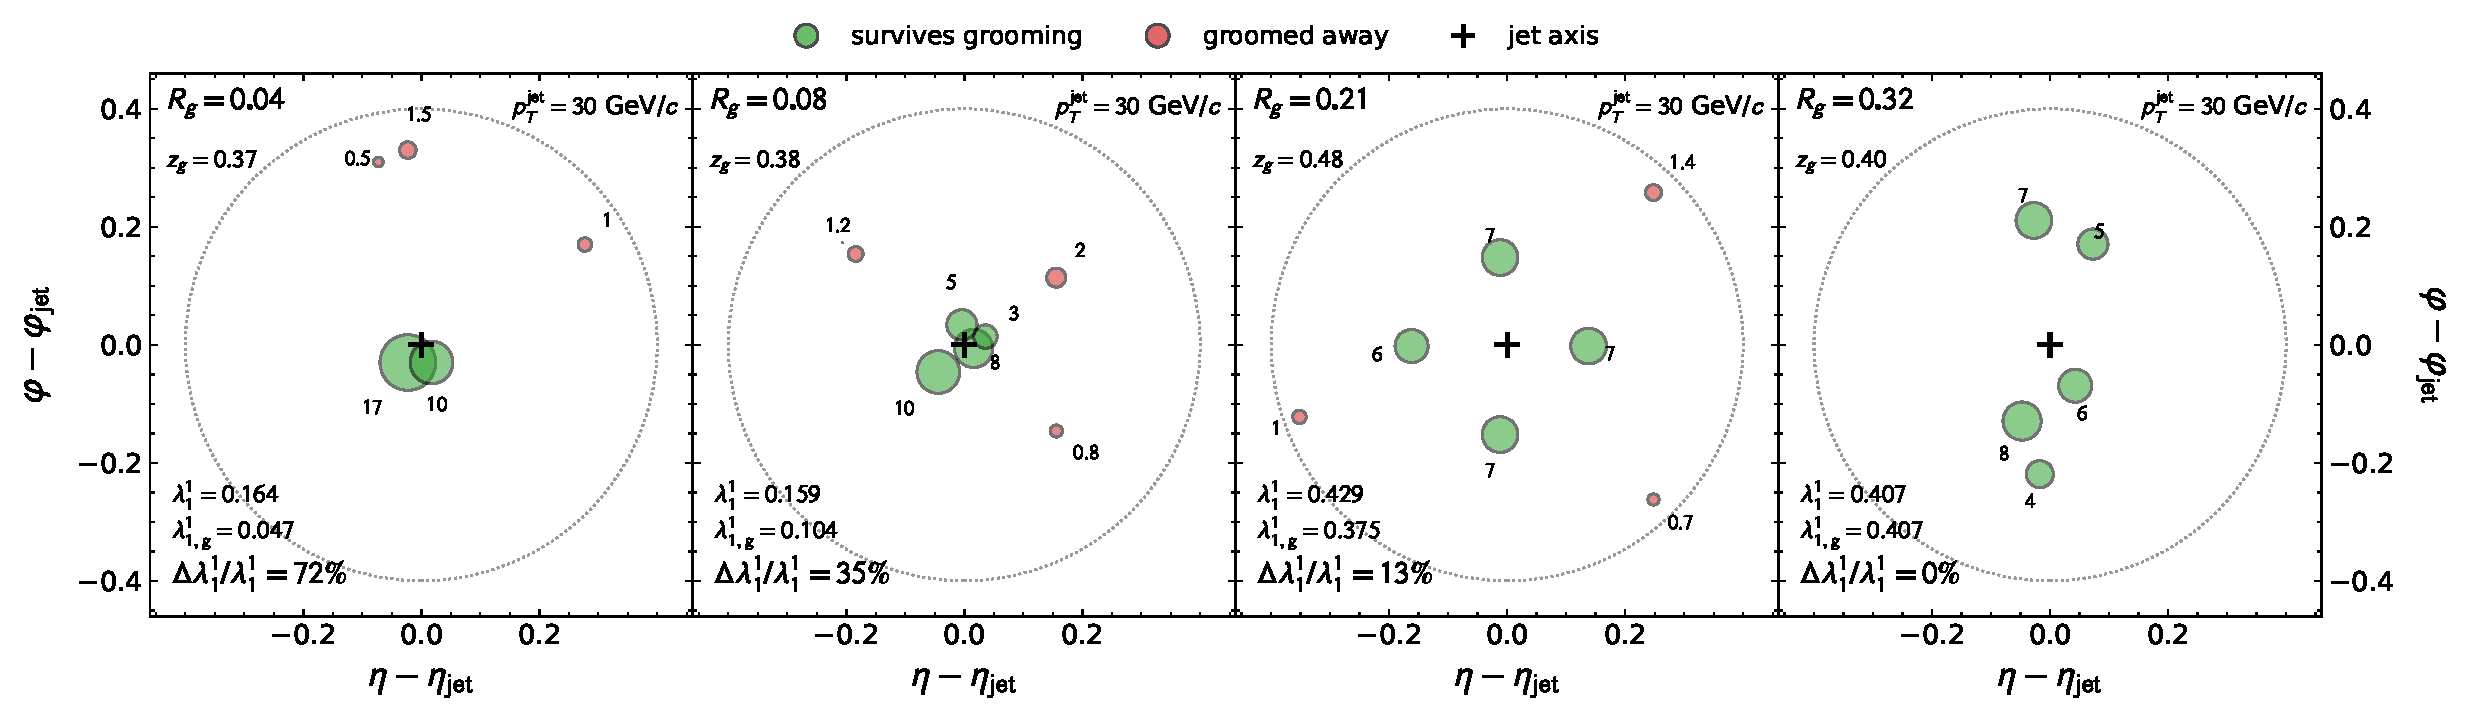
\includegraphics[width=\linewidth]{figures/fig_grooming_cartoon_4panel.pdf}
	\caption{ Ways of arranging constituents (each represented as a circle whose radius represent \(\frac{p_\mathrm{T, const}}{p_\mathrm{T, jet}}\)) in the \etaphi space within a jet with \(p_\mathrm{T, jet} = 30~\text{GeV}/c\) such that \(R_\mathrm{g}\) of the jet increases going from left to right. Green (Red) colored constituents survive (are removed by) the SoftDrop grooming ( \(z_\mathrm{cut} = 0.2,~\beta = 0\)).}
	\label{fig:GroomingAndRg}
\end{figure}

\subsection{Dataset and Methodology}
The analysis uses data from \pp collisions at \sPP{200}{GeV}~collected in 2012 using the STAR detector system. Charged-particle tracks and neutral energy depositions (towers) are measured using STAR's TPC and BEMC detectors respectively. 

To enhance jet signal, only High-Tower (HT) triggered events (at least one tower with $\EtTower \geq 4$ GeV) are considered. Events containing a track with \ptGeq{track}{30} are rejected to avoid contamination from cosmic rays, as in the Au+Au analysis (Sect.~\ref{sec:JHEventSel}). Tracks(Towers) with \ptGeq{track}{0.2} (\(E_\mathrm{T, tower} \geq 0.2\) GeV) are considered for jet clustering. The tracks pass the same quality criteria as in the Au+Au analysis (Tab.~\ref{Tab:JHTrackCuts}), bad and dead towers are removed, and the full momentum of the tracks matched to a tower is subtracted from its energy (Eq.~\ref{Eq:HadCorr}); the reasons for these choices are discussed in Sect.~\ref{sec:TrackTowerSel}. Clustered jets completely falling within acceptance ($|\eta_{\rm jet}| \leq 0.6$), with \ptGeq{jet}{10} and a plurality of charged tracks (\(N_\mathrm{ch., jet} \geq 2\)) are used for further study.  
%Jets with area, $A_{\rm jet} < 0.3$ are rejected to further reduce the fake jet contribution. 

 The tracks and towers are clustered into jets using the anti-\(k_{\rm T}\) algorithm with a jet resolution parameter $R = 0.4$, implemented using the FastJet library~\cite{Cacciari_2012}, with the same particle-mass assumptions and recombination scheme as in Sect.~\ref{sec:JetRecoAuAu}. Unlike the hard-core Au+Au jets, all tracks and towers above 0.2~GeV are clustered, so the jets are inclusive.  After obtaining the jets, the softer constituents are groomed using Recursive SoftDrop with \(\beta = 0\) and \(z_\mathrm{cut} = 0.2\). The groomed-jet's constituents lose non-kinematic information like charge, which is regained by matching them to the original jet's constituents. 
 
 \subsection{Detector effects and Unfolding}
 The embedding simulation starts from PYTHIA6 (STAR Tune)  at the particle level. The particles are then reconstructed as detector hits using the STAR detector system implemented in GEANT3 and embedded into zero-bias events from 200 GeV \pp collisions (2012). The jets from particle and detector levels are matched using a \(p_\mathrm{T, jet}\) ordered nearness criteria, similar to the one used for the Au+Au embedding (Sect.~\ref{sec:AuAuEmbedding}).  The matched jets can be used to show detector responses like shown in Fig.~\ref{fig:PtResolution} (top) and  \(p_\mathrm{T, jet}\)-resolution (Eq.~\ref{Eq:JetPtRes}) shown in Fig.~\ref{fig:PtResolution} (bottom).  


 \begin{figure}
 	\centering
 	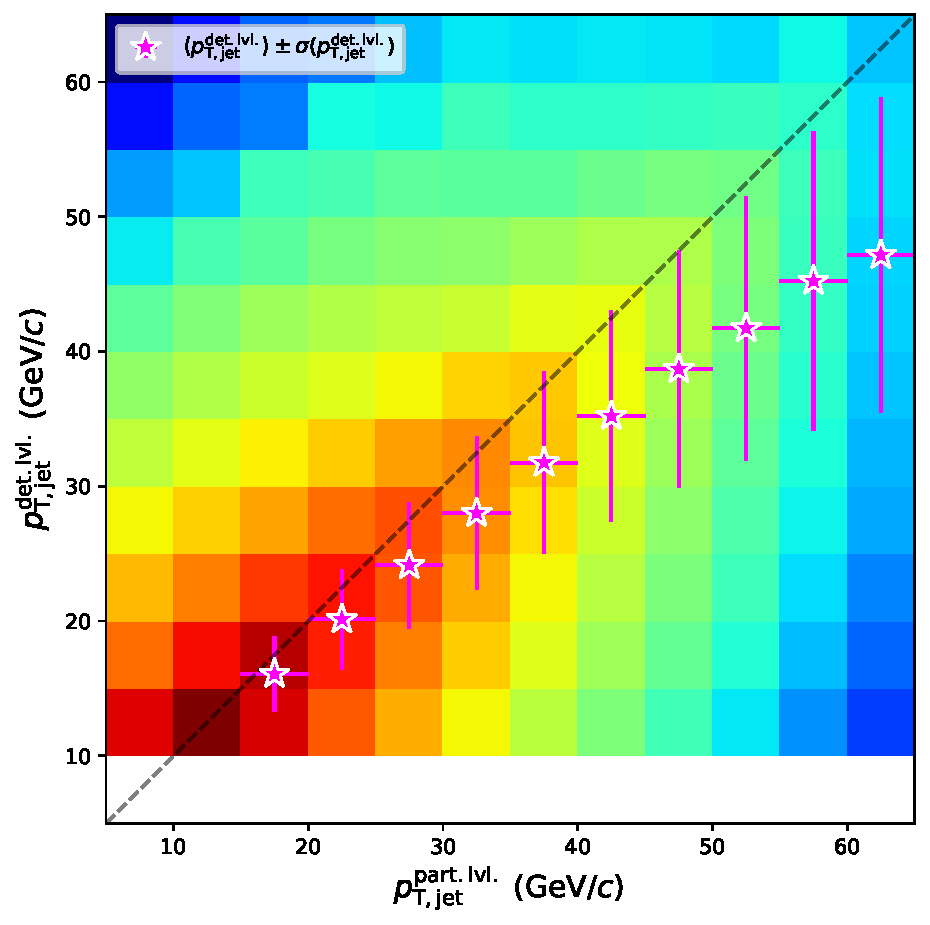
\includegraphics[width=0.5\linewidth]{figures/jet_pt_response.pdf}
 	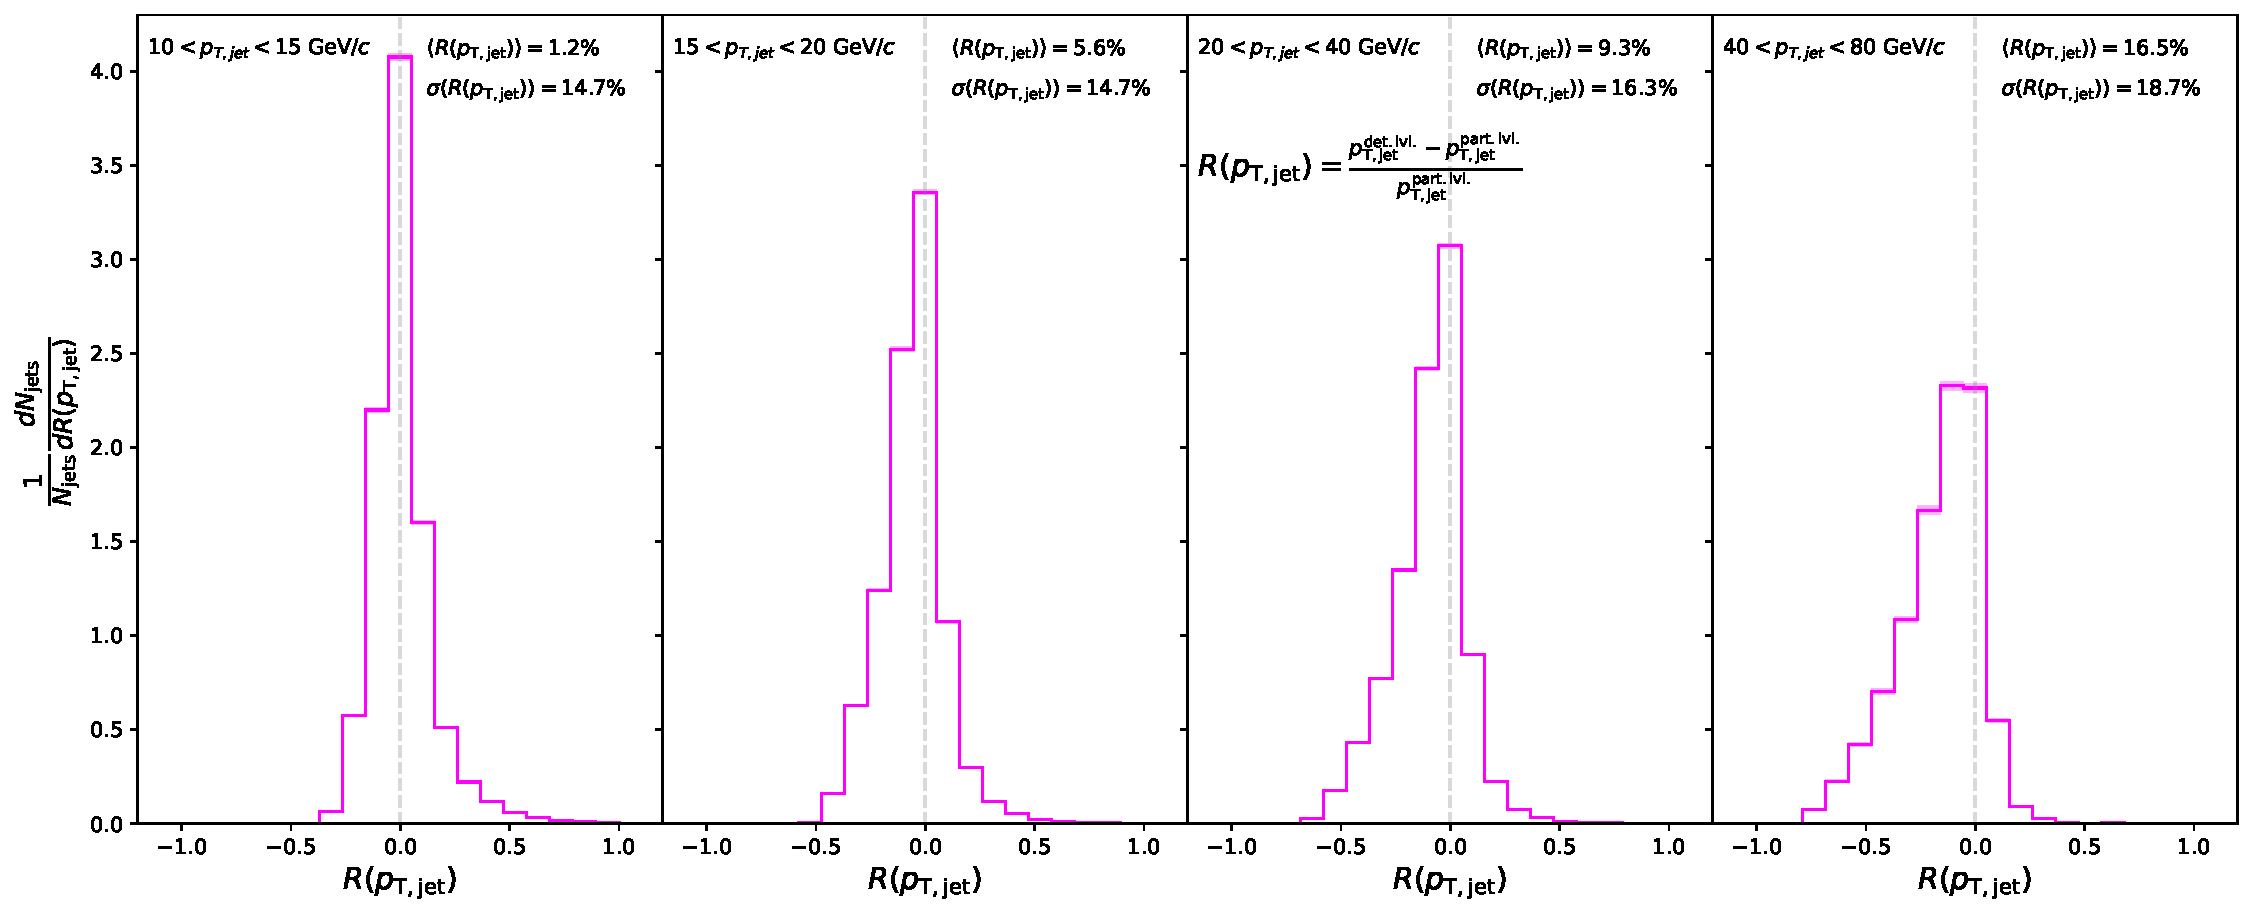
\includegraphics[width=\linewidth]{figures/jet_pt_res.pdf}
 	\caption{Jet-\(p_\mathrm{T}\) response of the PYTHIA-6 + GEANT3 embedding for matched jets. (Top) Probability of a particle-level jet with \ptGenJet to be reconstructed with \ptRecoJet; the magenta stars are the mean \ptRecoJet in each bin of \ptGenJet, with the standard deviation as error bars. (Bottom) Distributions of the relative difference \(R(p_\mathrm{T, jet}) = (p_\mathrm{T, jet}^\mathrm{det.} - p_\mathrm{T, jet}^\mathrm{part.})/p_\mathrm{T, jet}^\mathrm{part.}\) in four ranges of \(p_\mathrm{T, jet}^\mathrm{part.}\); their mean and standard deviation, quoted in each panel, are the jet-\(p_\mathrm{T}\) scale shift and resolution.}
 	\label{fig:PtResolution}
 \end{figure}
 
 Unfolding is done using the Multifold method. Every jet is represented as a vector of 23 features. The four classifiers of Multifold are parametrized as DNNs with 3 hidden layers with 256 nodes each. The model weights are trained using the AdamW optimizer with a learning rate of \(10^{-3}\) and weight decay of \(10^{-2}\). Convergence is achieved in two unfolding iterations. Statistical uncertainties are calculated using bootstrap ensemble with 50 model replicas each sub-sampling  500k each of the data-like and sim-like jets, so each model replica sees 1M jets every epoch. All the  required unfolded distributions and profiles are calculated by using the per-jet unfolding weights. 
 
 \begin{figure}
 	\centering
 	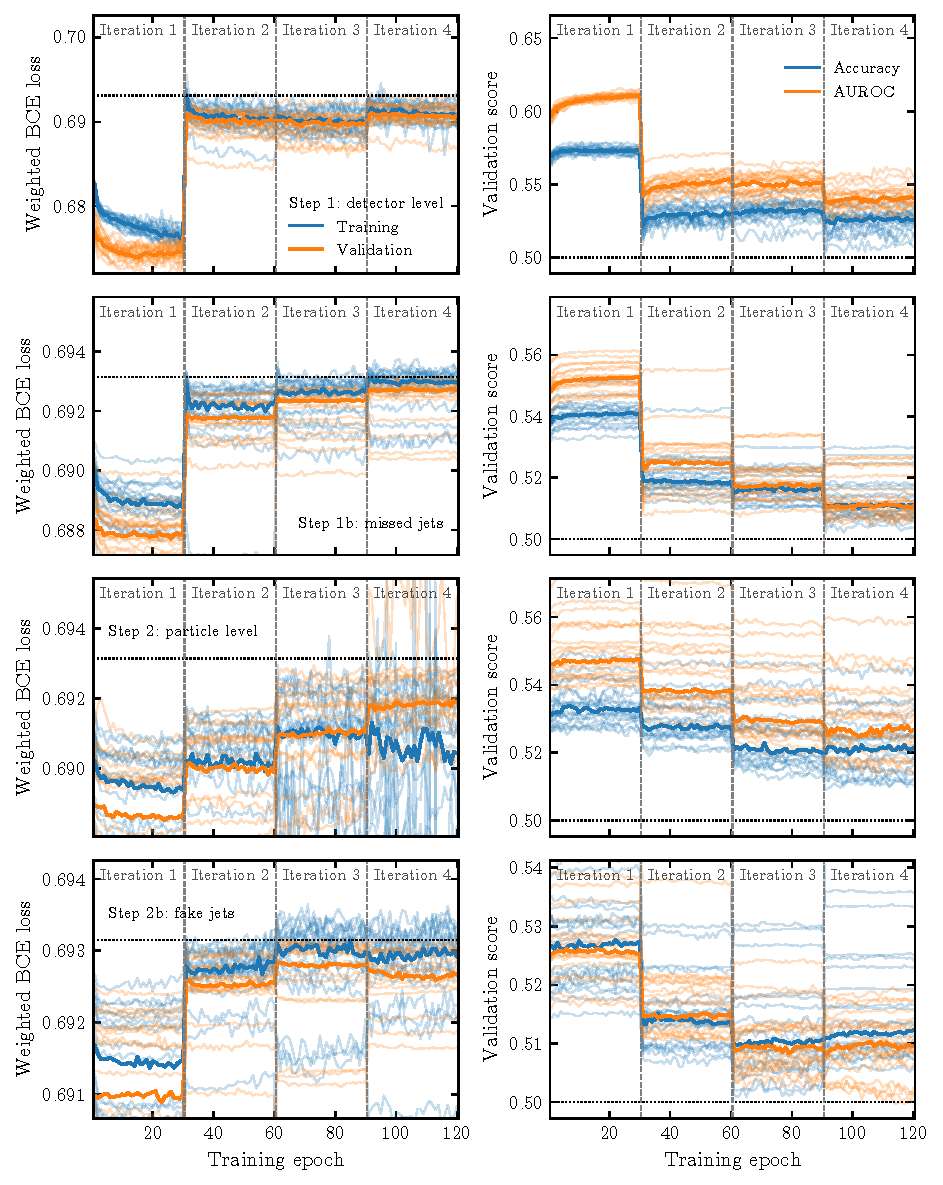
\includegraphics[width=\linewidth]{figures/angularities/pp/unfolding/training_all.pdf}
 	%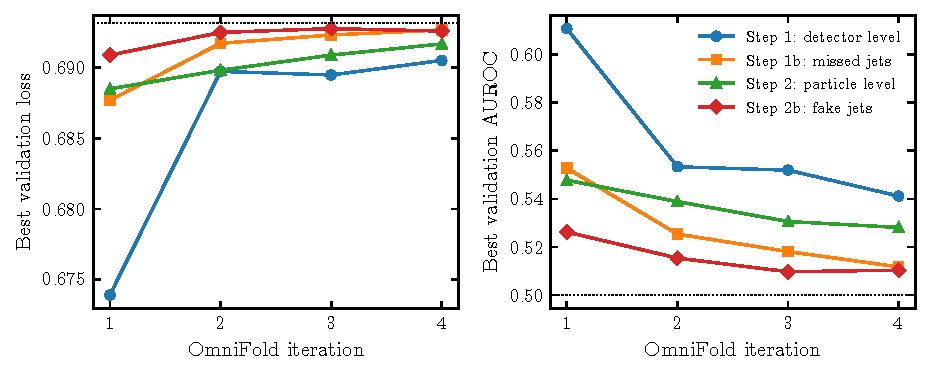
\includegraphics[width=0.49\linewidth]{figures/angularities/pp/unfolding/training_summary.pdf}
 	\caption{Training history of the four MultiFold classifiers over four iterations of 30 epochs each: step 1 (detector level, measured vs.\ reconstructed jets), step 1b (missed jets), step 2 (particle level) and step 2b (fake jets), from top to bottom. (Left) Weighted binary cross-entropy loss on the training (blue) and validation (orange) samples. (Right) Accuracy (blue) and area under the ROC curve (AUROC, orange) on the validation sample. Thin lines are the individual ensemble replicas and thick lines their median; the dotted lines mark a classifier with no separating power (loss \(\ln 2\), score 0.5). The nominal result uses the second iteration.}
 	\label{fig:unfoldigLossAccAUC}
 \end{figure}
 
 Closure test of the unfolding shown in  Fig. \ref{fig:ClosureAngularity} and \ref{fig:ClosureAngVsRg} is done by doing the same unfolding procedure replacing measured data with pseudo-data for which the particle level is known (pseudo-truth). The pseudo-unfolded distributions are then compared to the pseudo-truth via ratios
 \begin{figure}
 	\centering
 	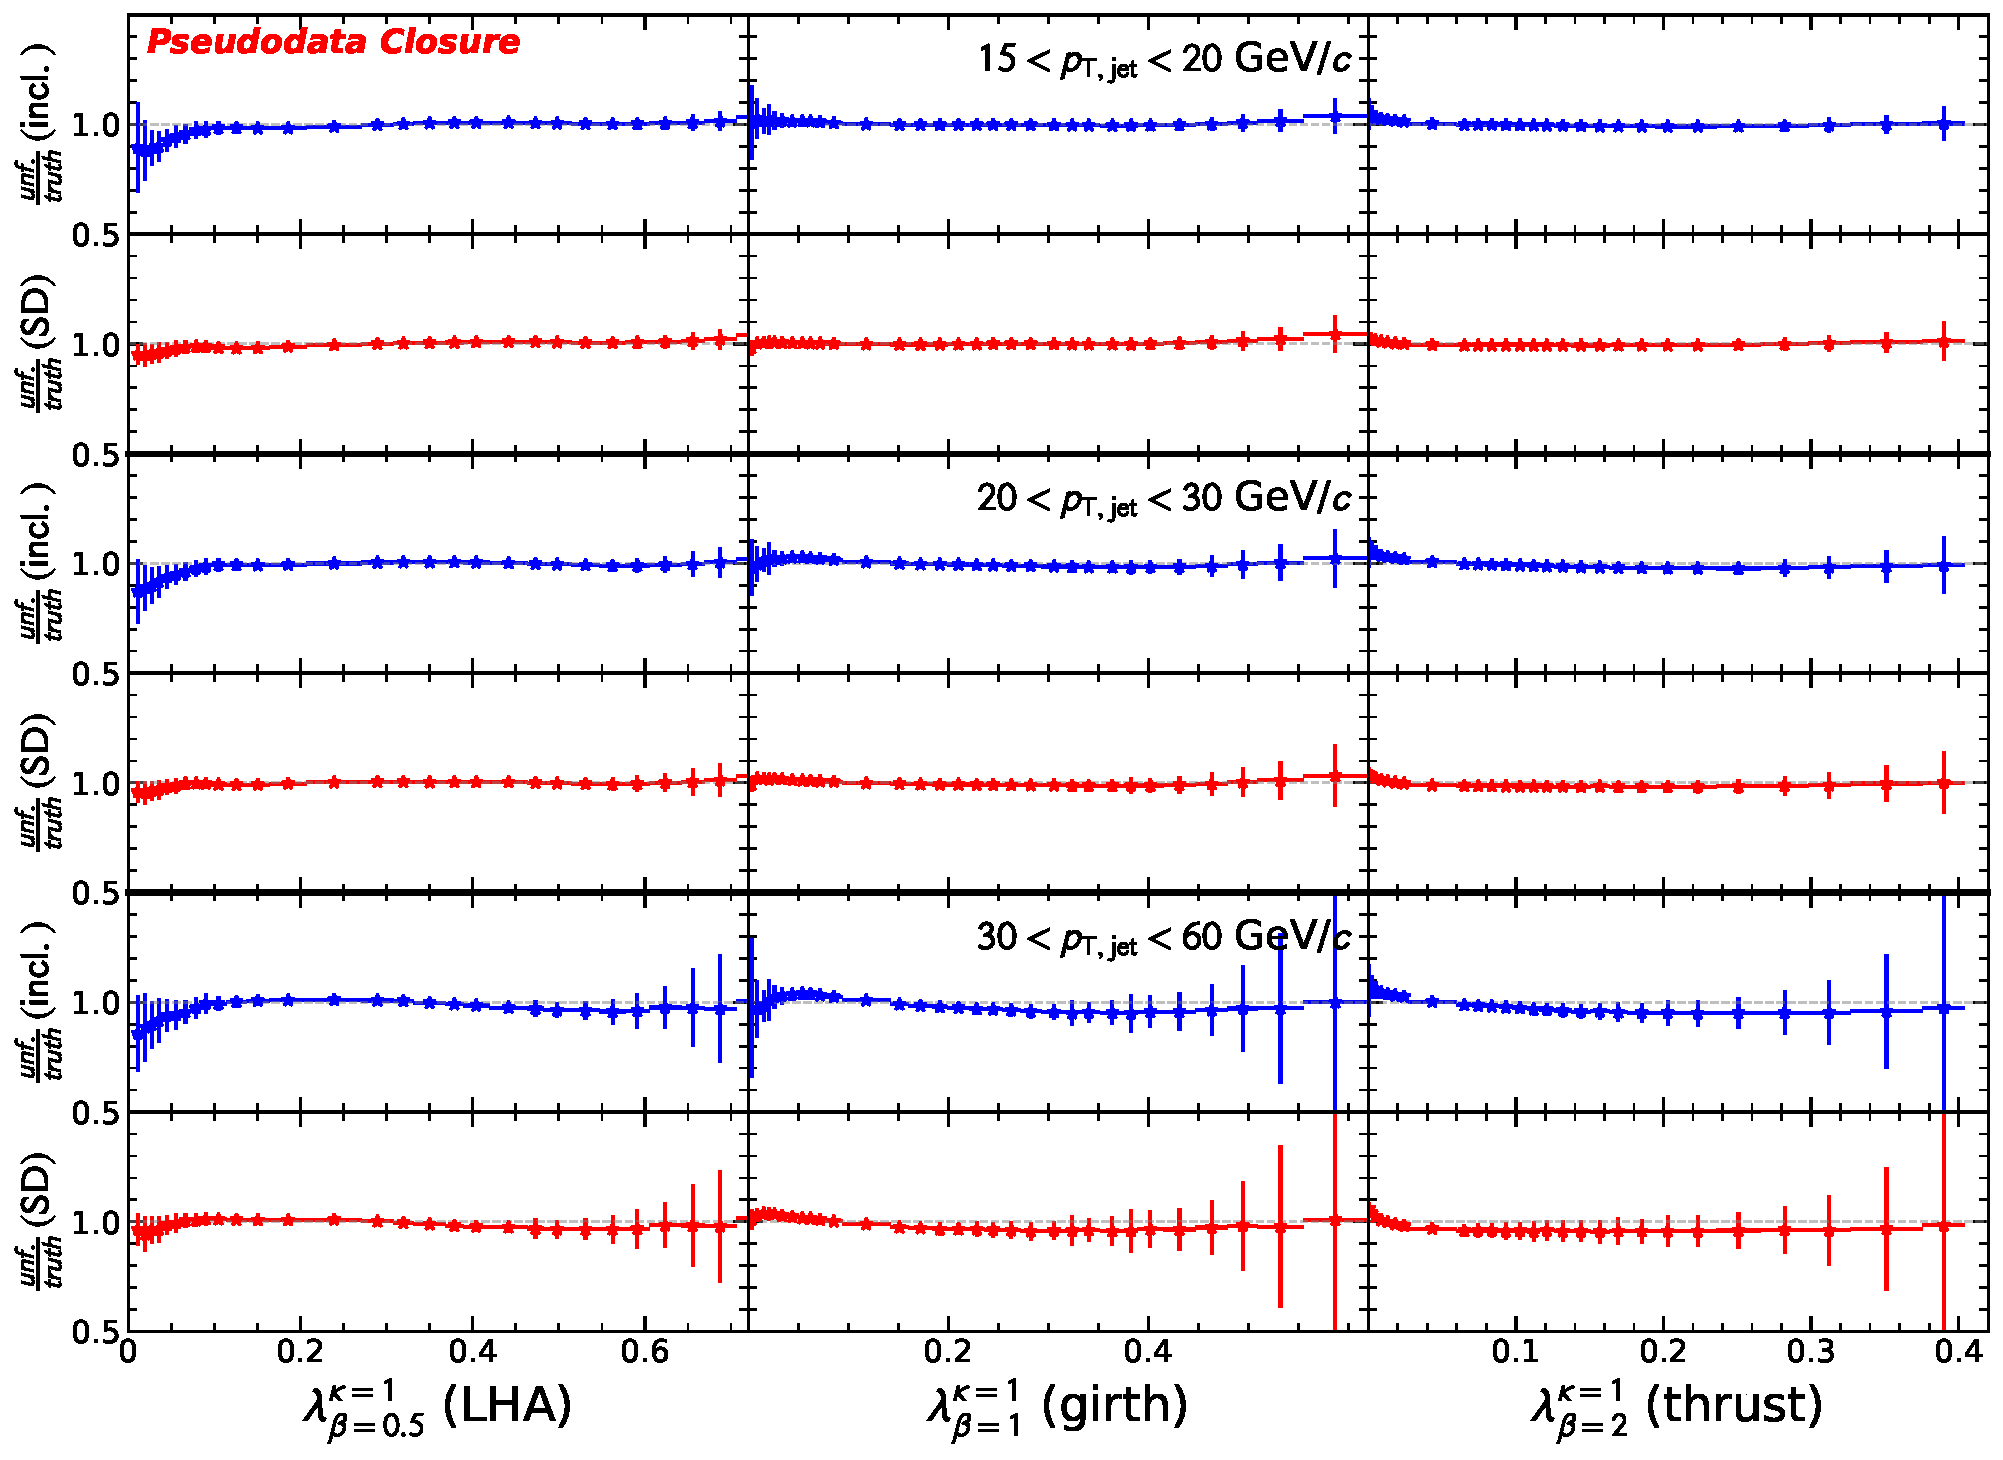
\includegraphics[width=\linewidth]{figures/angularities/pp/fig_dist_ptbins_closure_like.pdf}
 	\caption{Closure test with the data-like prior: ratio of the pseudo-unfolded to the pseudo-truth distributions of \(\lambda^{\kappa=1}_{\beta}\) for \(\beta = 0.5\) (LHA, left), 1 (girth, middle) and 2 (thrust, right), for inclusive (blue) and SoftDrop-groomed (red) jets, in three \(p_\mathrm{T, jet}\) ranges (rows). Error bars are the statistical uncertainties.}
 	\label{fig:ClosureAngularity}
 \end{figure}
 
 \begin{figure}
 	\centering
 	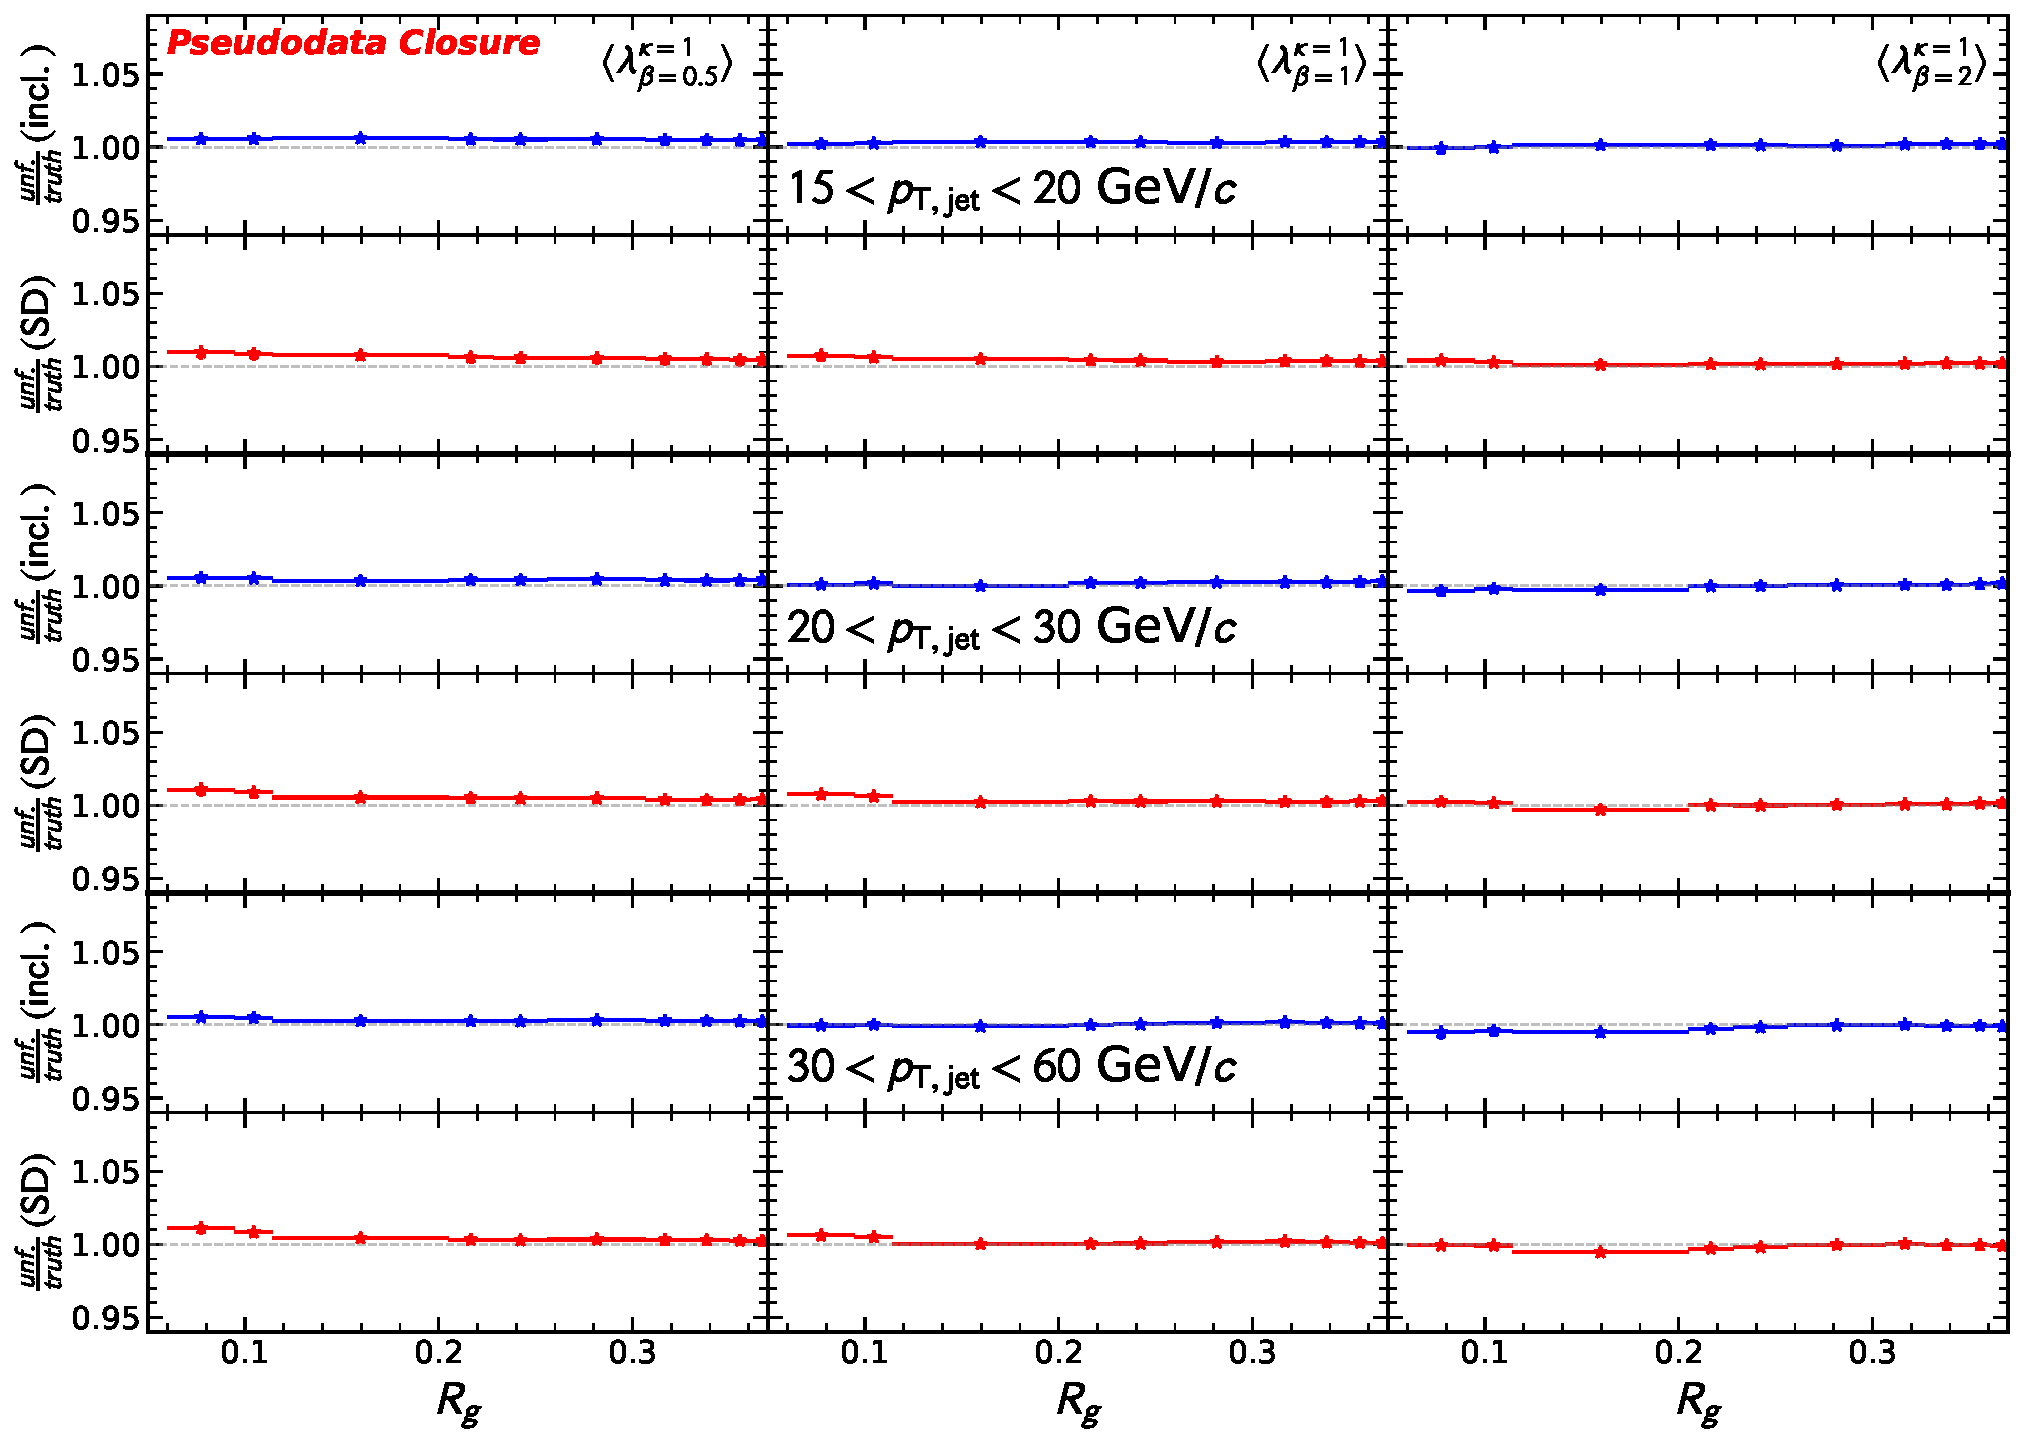
\includegraphics[width=\linewidth]{figures/angularities/pp/fig_dr_ptbins_closure_like.pdf}
 	\caption{Closure test with the data-like prior for the \(\langle\lambda^{\kappa=1}_{\beta}\rangle\) vs.\ \(R_\mathrm{g}\) profiles: ratio of the pseudo-unfolded to the pseudo-truth profiles for \(\beta = 0.5\) (left), 1 (middle) and 2 (right), for inclusive (blue) and SoftDrop-groomed (red) jets, in three \(p_\mathrm{T, jet}\) ranges (rows). Error bars are the statistical uncertainties.}
 	\label{fig:ClosureAngVsRg}
 \end{figure}
 
 \subsection{Statistical Uncertainties}
 \label{sec:bootstrap}
 The classifiers of the previous section are trained on finite samples of measured, reconstructed and generated jets, and the training itself is stochastic through the initialization of the model, dropout and the order of the mini-batches. 
 %
 The unfolded distribution inherits all of these, and after several trainings chained across iterations there is no closed form for propagating them. 
 %
 Instead, the whole procedure is repeated on resampled inputs and the spread of the outcomes is taken as the uncertainty. 
 
 Every classifier \(f\) is replaced by an ensemble of \(N_\mathrm{rep.}\) replicas. 
 %
 Replica \(r\) is trained on a random subsample of \(m\) jets drawn without replacement from each of the two classes it separates (e.g. \(m\) measured and \(m\) reconstructed jets for \(f_\mathrm{meas., reco}\)), split further into a training and a validation set, with its own initialization and dropout. 
 %
 The same replica index is carried through every classifier of every iteration, so replica \(r\) is a complete unfolding on its own, with weights \(\omega^{(r)}_{n-1}\) and \(\nu^{(r)}_{n-1}\) and, from eq.~\ref{eq:generalUnfolding},
 \begin{equation}
 	\label{eq:replicaWeight}
 	p^{(r)}_{\mathrm{gen.}, n}(\mathbf{x}) = p_{\mathrm{gen.}, 0}(\mathbf{x})\prod_{k=0}^{n-1}\nu^{(r)}_k(\mathbf{x}) \equiv w^{(r)}_n(\mathbf{x})\,p_{\mathrm{gen.}, 0}(\mathbf{x})
 \end{equation}
 Where, \(w^{(r)}_n(\mathbf{x})\) is the per-jet unfolding weight of replica \(r\) after \(n\) iterations. 
 %
 The subsampling is only done for training; at inference every replica is evaluated on every jet, so eq.~\ref{eq:replicaWeight} gives \(N_\mathrm{rep.}\) unfolded samples, each with the full statistics of the simulation. 
 
 Any binned quantity \(H\), a histogram, a profile or a ratio of two of them, is then calculated once per replica from the weights \(w^{(r)}_n\), and its central value and uncertainty are the mean and standard deviation over the ensemble,
 \begin{equation}
 	\label{eq:bootstrapUnc}
 	\bar{H} = \frac{1}{N_\mathrm{rep.}}\sum_{r=1}^{N_\mathrm{rep.}} H^{(r)} , \qquad
 	\sigma_H^2 = \frac{1}{N_\mathrm{rep.} - 1}\sum_{r=1}^{N_\mathrm{rep.}}\left(H^{(r)} - \bar{H}\right)^2 
 \end{equation}
 Ratios are formed replica by replica before averaging, so the correlation between numerator and denominator through the shared weights is kept. 
 %
 Where a single diverged replica would pull \(\bar{H}\), the median or a trimmed mean over the ensemble is used for the central value instead; \(\sigma_H\) is always the standard deviation. 
 
 Since the replicas differ in the measured subsample, the simulated subsample and the training, \(\sigma_H\) contains the statistical uncertainty of the measurement, that of the simulation and the variance of the training procedure, without separating them. 
 %
 With \(m\) smaller than the full samples, the spread is that of samples of size \(m\) and is conservative for the purely statistical part. 
 %
 \(N_\mathrm{rep.}\) only sets how precisely \(\sigma_H\) itself is known, not its size. 
 
 \subsection{Systematic Uncertainties}
 \subsubsection{Jet Reconstruction Related Uncertainties}
 Analysis was rerun with each of the following changes (compared to the nominal) done to the detector level of the embedding simulation.  
 %
 The differences in the final plots for the source was calculated. 
 %
The Barlow test was performed on each source of systematic error to remove the statistical fluctuation from the variation.
%
The relative uncertainty from every source, detector and unfolding related, is shown before the Barlow check in Figs.~\ref{fig:SysDistInclRaw}--\ref{fig:SysProfSDRaw} and after it in Figs.~\ref{fig:SysDistIncl}--\ref{fig:SysProfSD}, for the inclusive and groomed distributions and for the \(\langle\lambda^{\kappa=1}_{\beta}\rangle\) vs.\ \(R_\mathrm{g}\) profiles.
\begin{figure}
	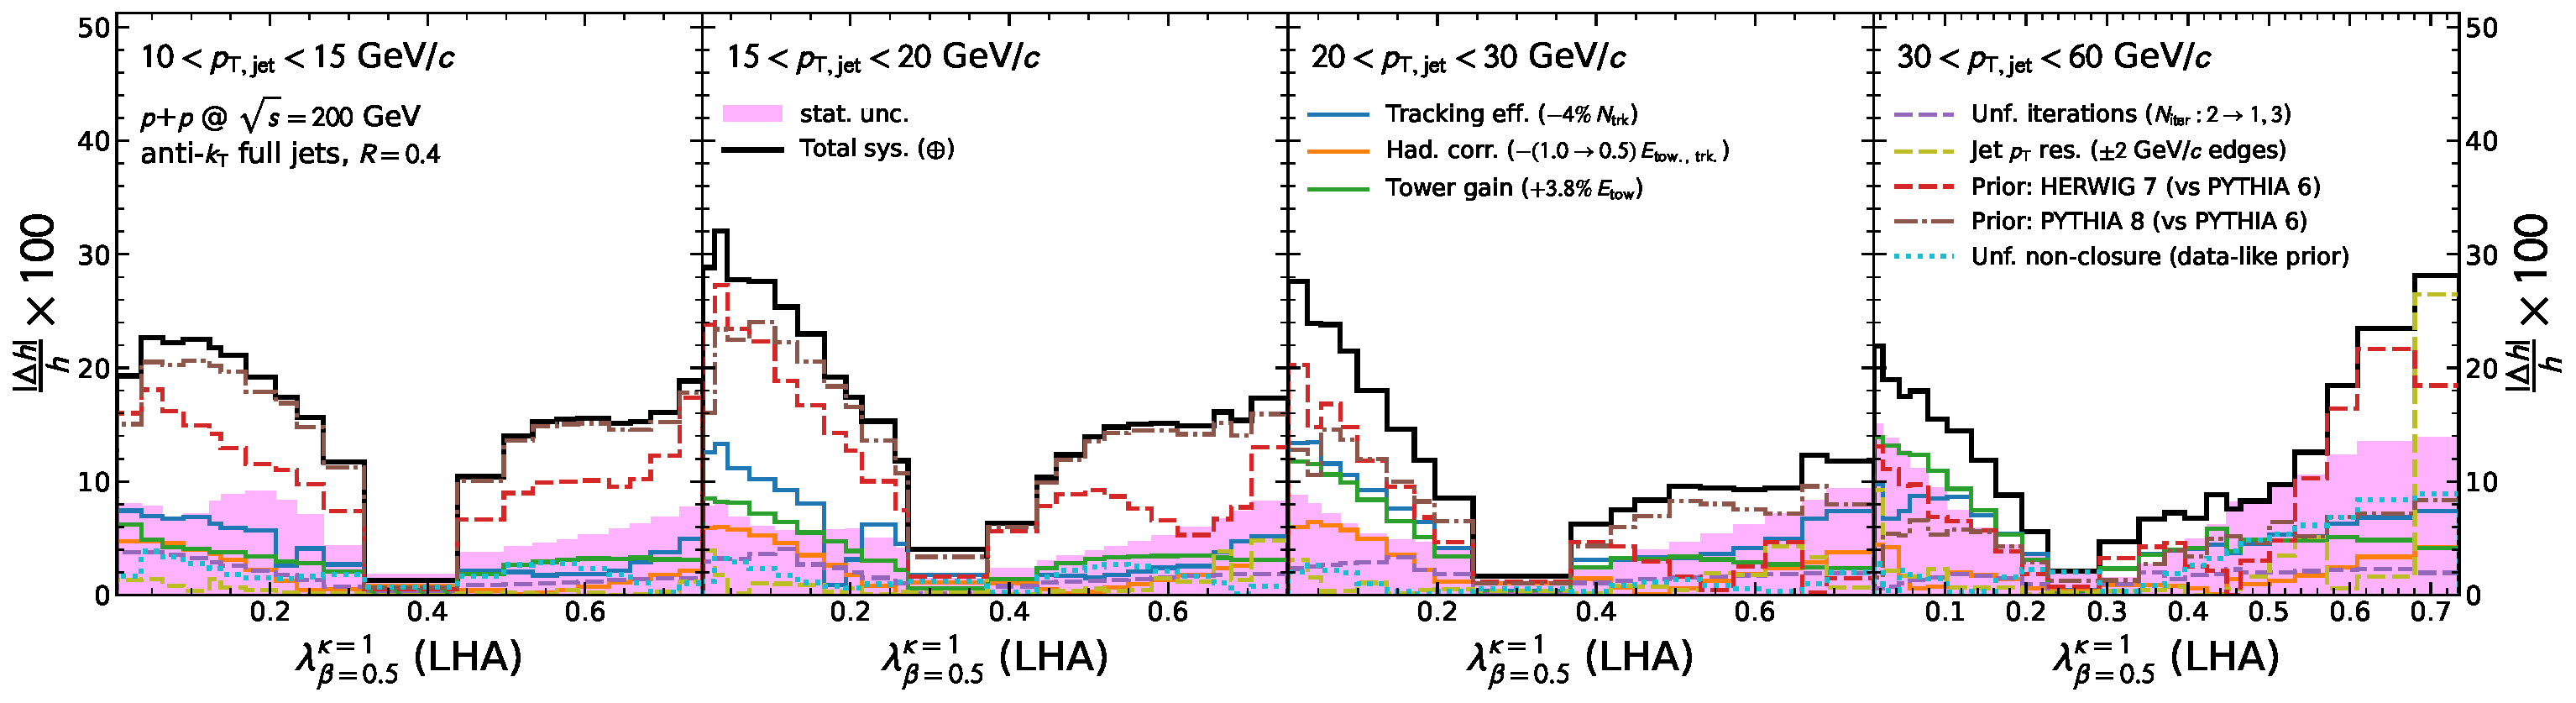
\includegraphics[width=\textwidth]{angularities/pp/sys_ch_ang_k1_b0.5_hist_ang_raw.pdf}
	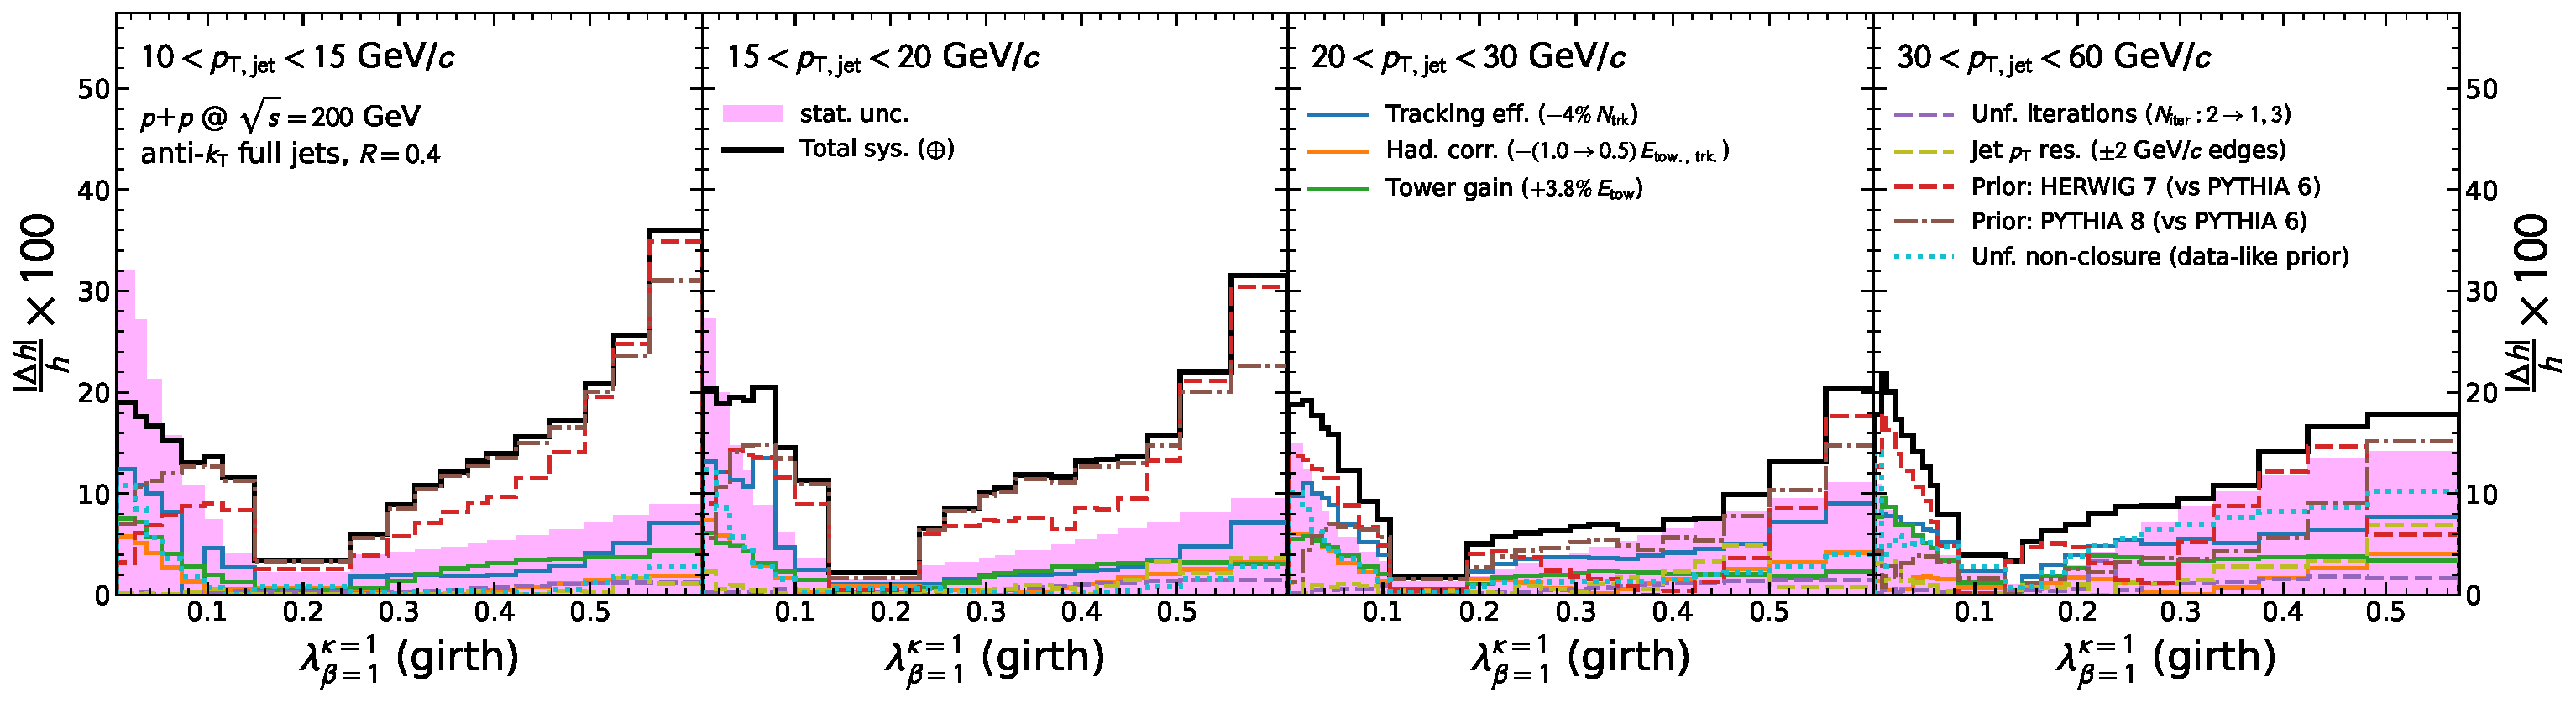
\includegraphics[width=\textwidth]{angularities/pp/sys_ch_ang_k1_b1_hist_ang_raw.pdf}
	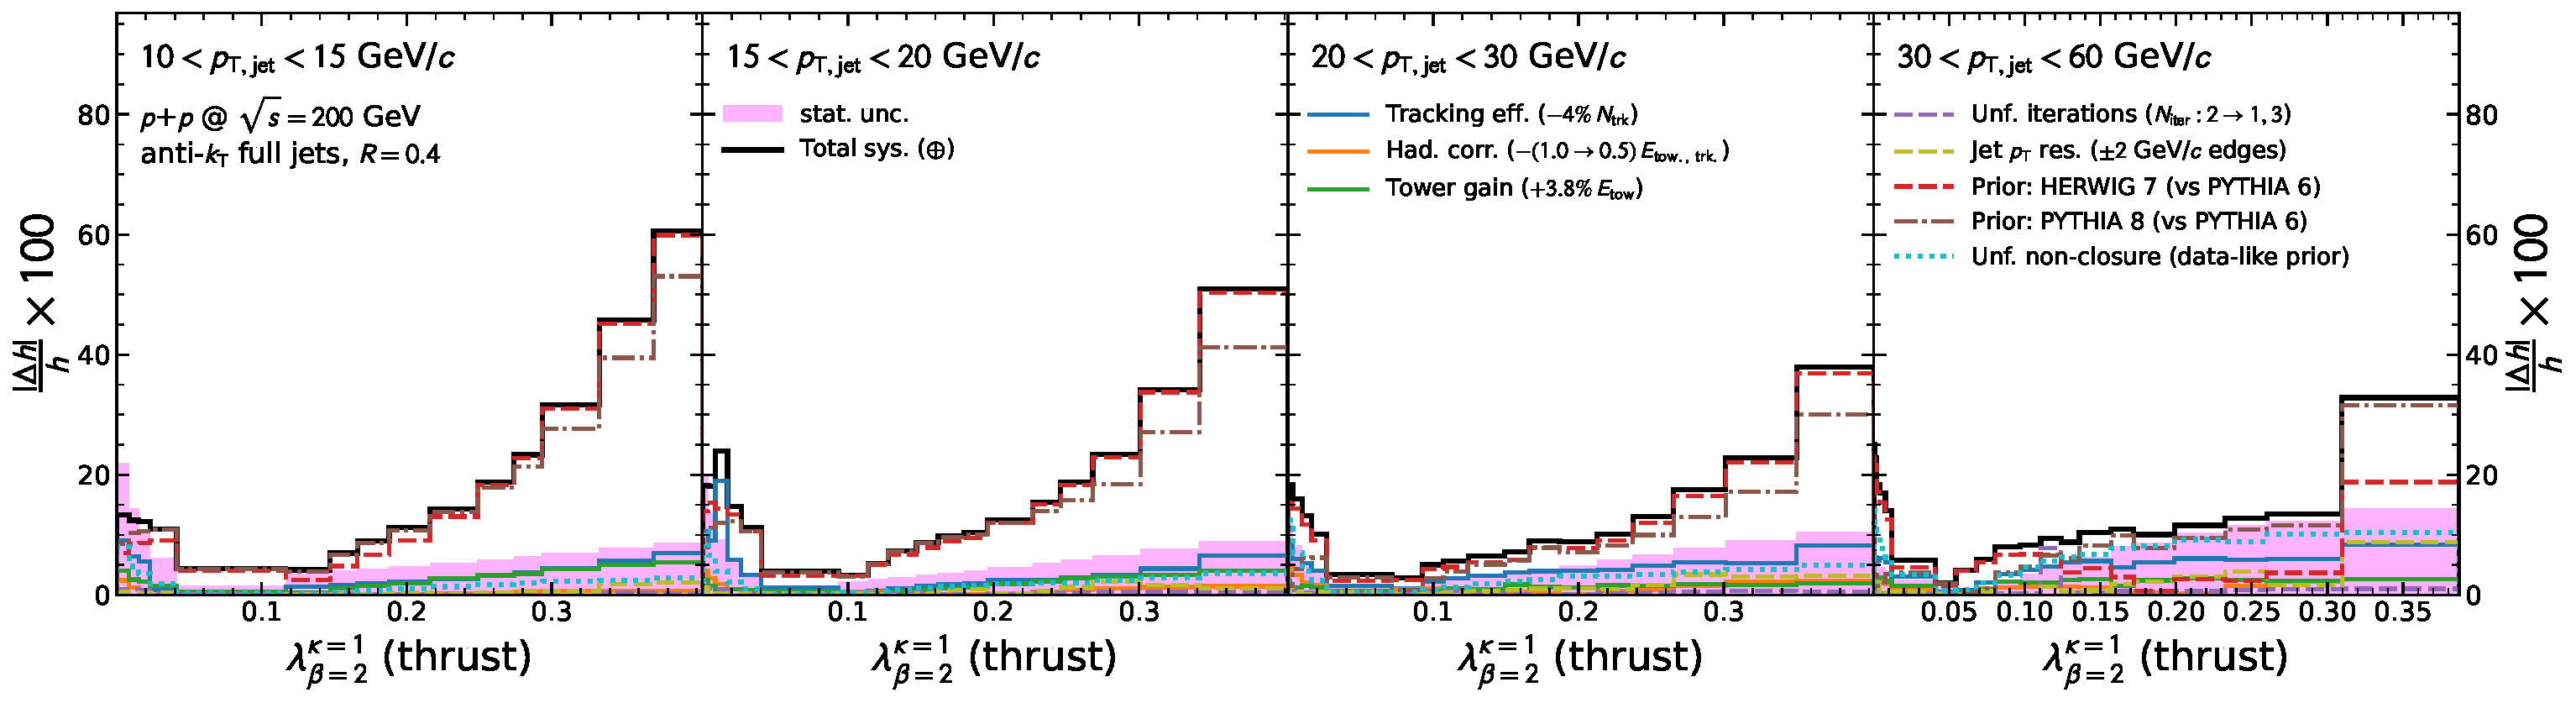
\includegraphics[width=\linewidth]{angularities/pp/sys_ch_ang_k1_b2_hist_ang_raw.pdf}
	\caption{Relative systematic uncertainties of the \(\lambda^{\kappa=1}_{\beta}\) distributions of inclusive jets, before the Barlow check (Sec.~\ref{sec:barlow}), for \(\beta = 0.5\), 1 and 2 (top to bottom). The sources are the tracking efficiency, the hadronic correction and the tower gain (solid), the number of unfolding iterations, the jet-\(p_\mathrm{T}\) resolution and the HERWIG-7 and PYTHIA-8 priors (dashed), and the non-closure (dotted); the black line is their sum in quadrature and the magenta band is the statistical uncertainty. Jet-\(p_\mathrm{T}\) ranges are shown as panels.}
	\label{fig:SysDistInclRaw}
\end{figure}
\begin{figure}
	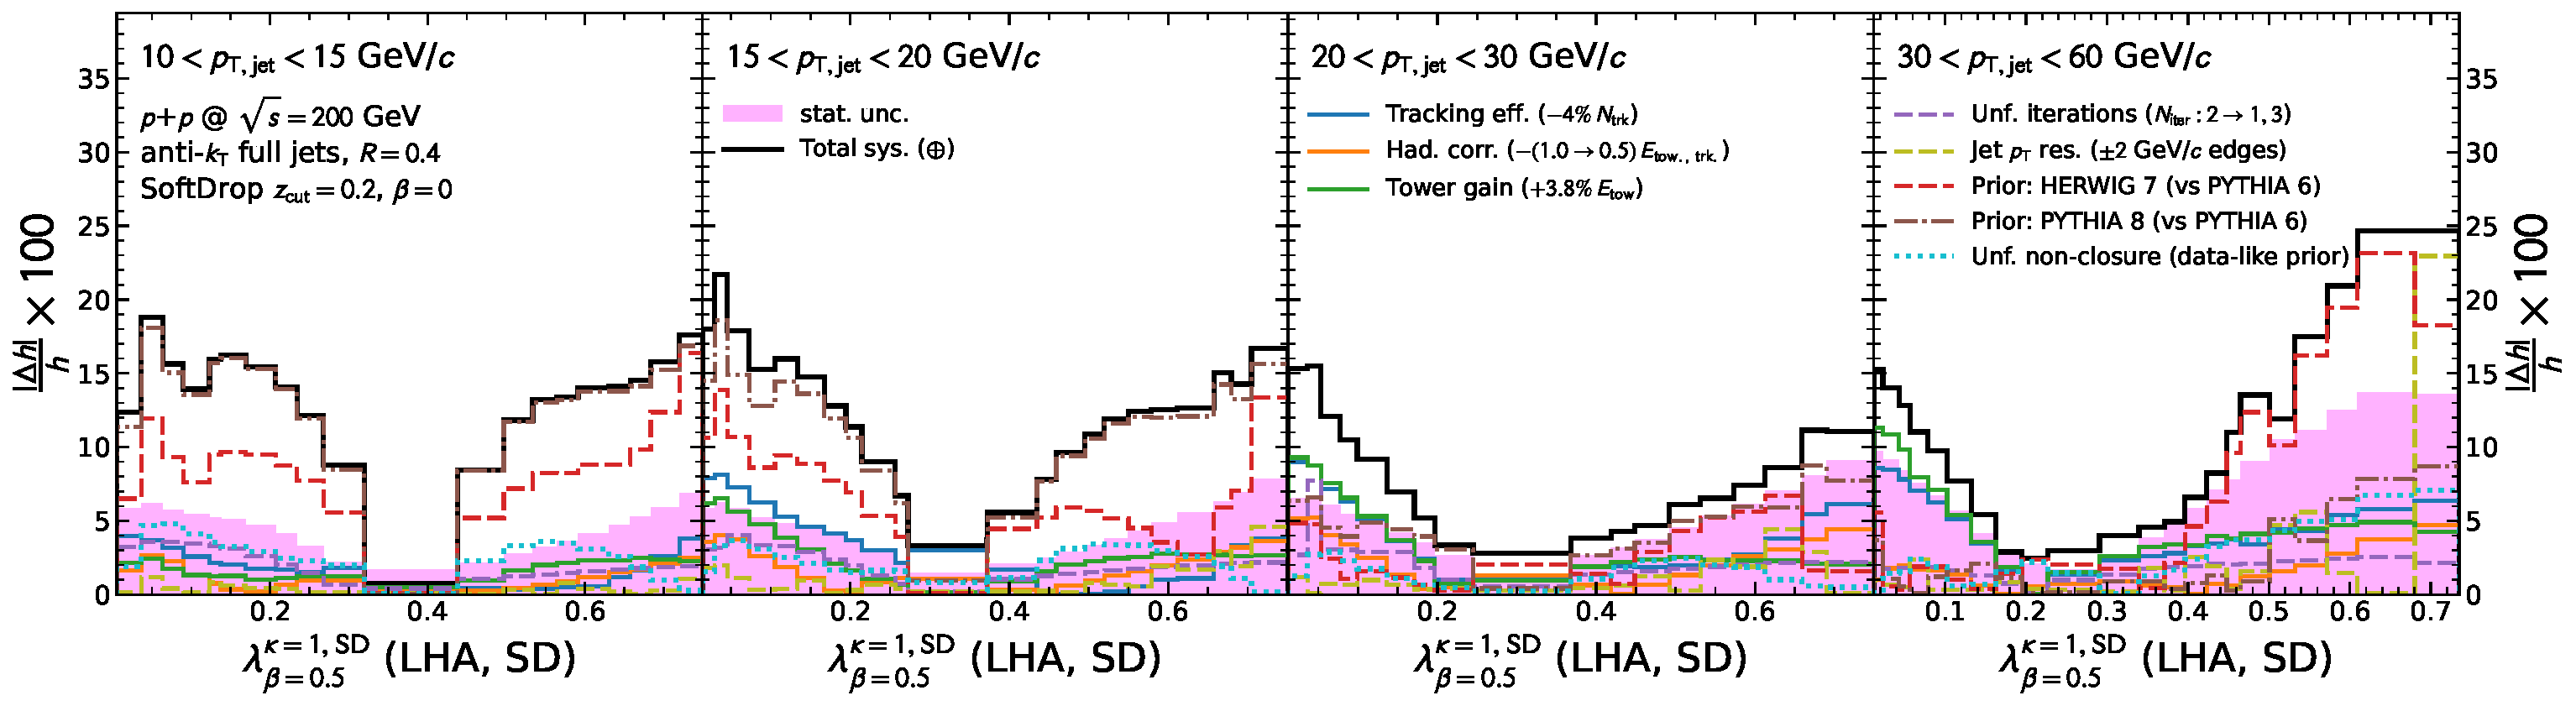
\includegraphics[width=\linewidth]{angularities/pp/sys_ch_ang_k1_b0.5_hist_sd_ang_raw.pdf}
	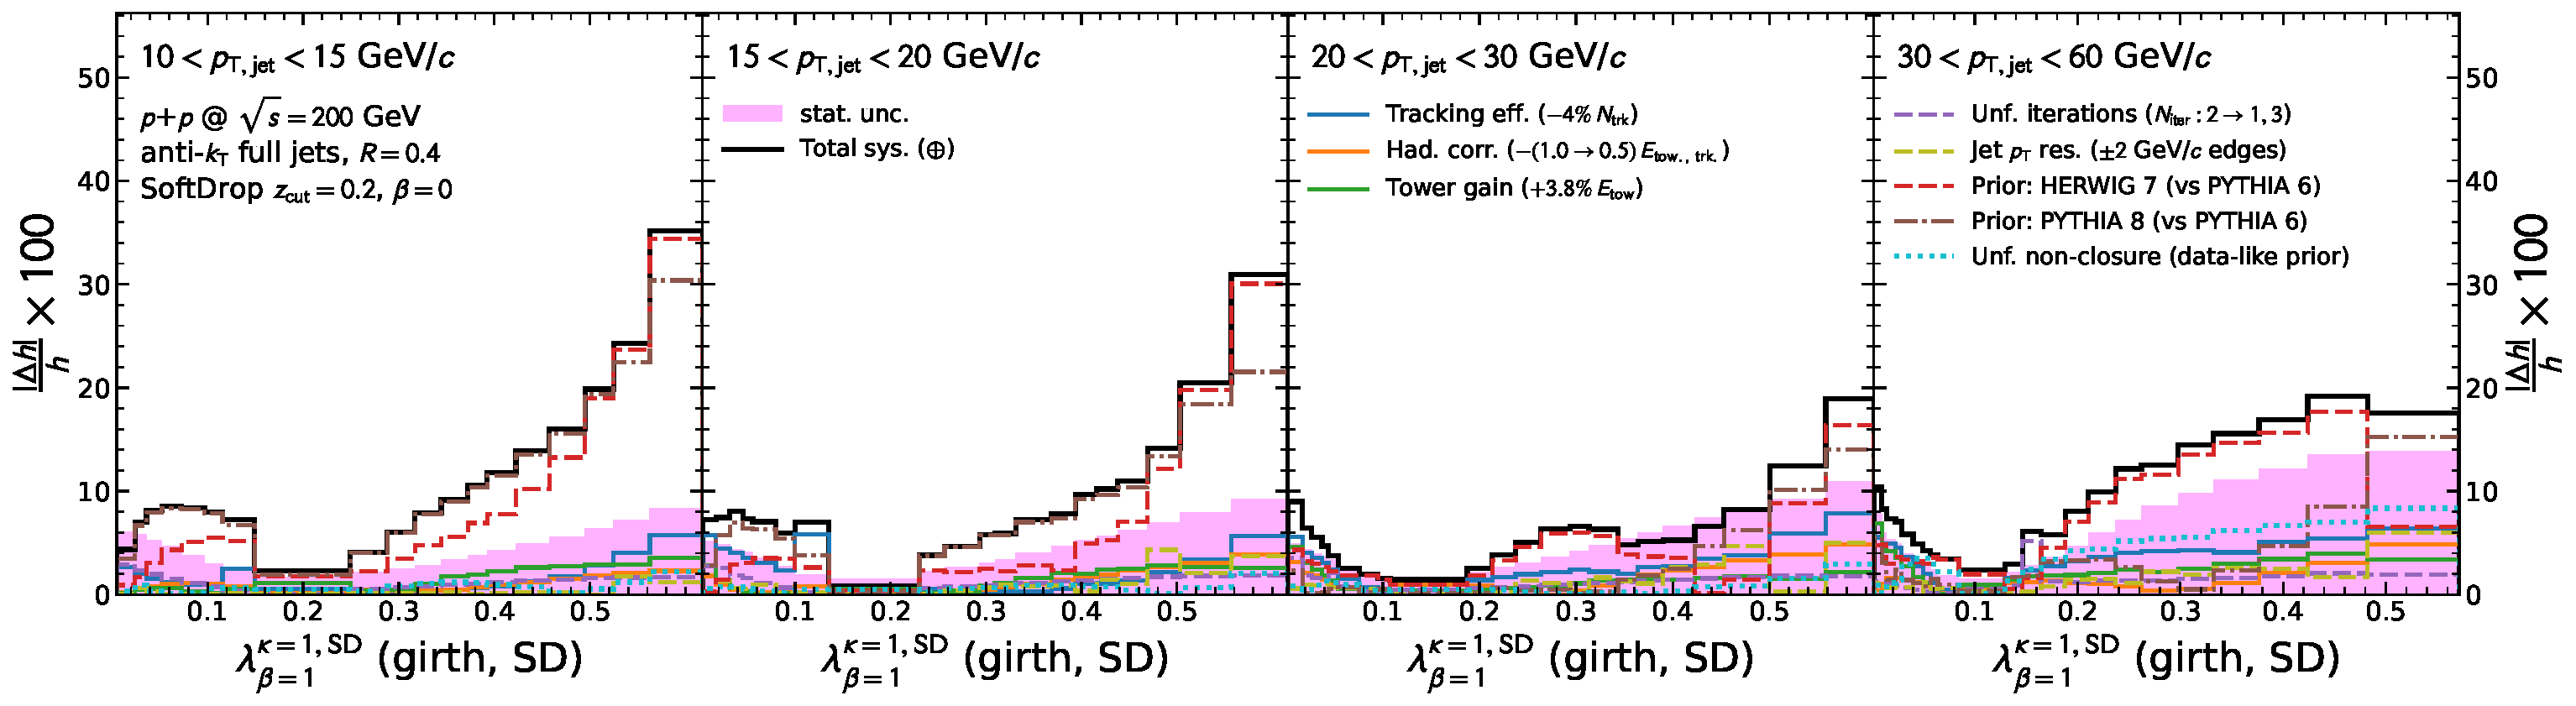
\includegraphics[width=\linewidth]{angularities/pp/sys_ch_ang_k1_b1_hist_sd_ang_raw.pdf}
	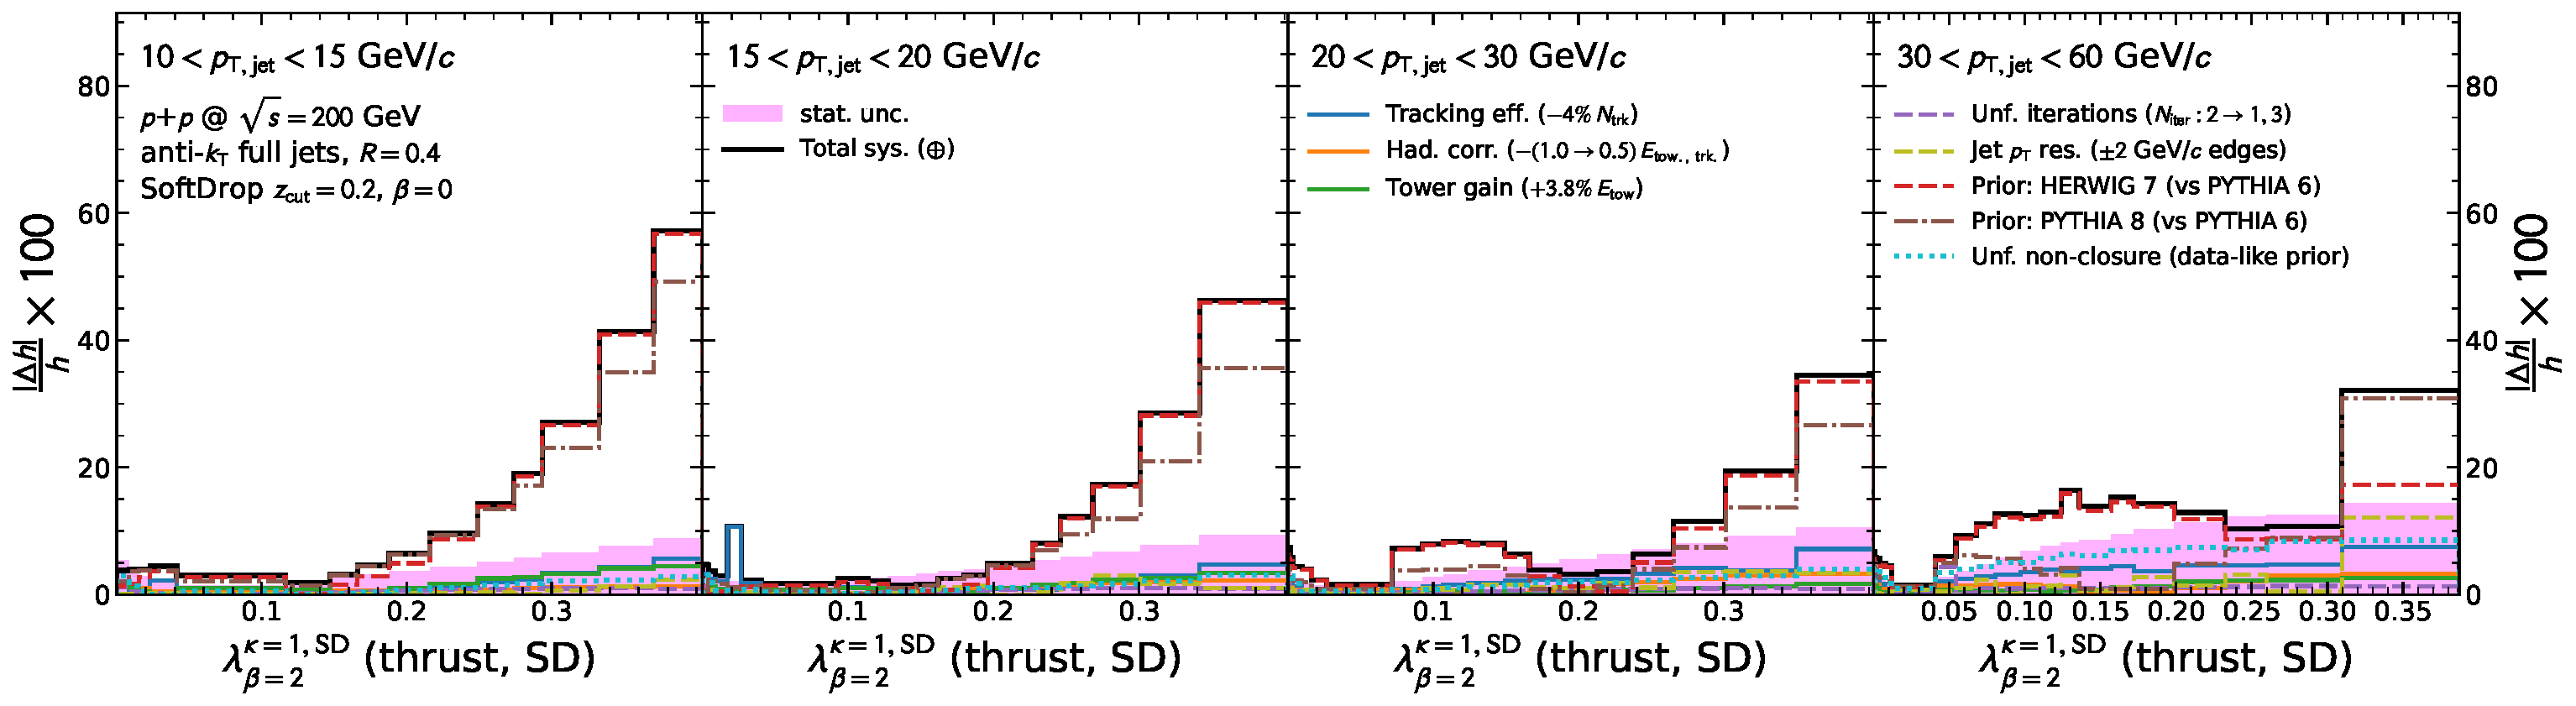
\includegraphics[width=\linewidth]{angularities/pp/sys_ch_ang_k1_b2_hist_sd_ang_raw.pdf}
	\caption{Relative systematic uncertainties of the \(\lambda^{\kappa=1}_{\beta}\) distributions of SoftDrop-groomed jets, before the Barlow check (Sec.~\ref{sec:barlow}), for \(\beta = 0.5\), 1 and 2 (top to bottom). The sources are the tracking efficiency, the hadronic correction and the tower gain (solid), the number of unfolding iterations, the jet-\(p_\mathrm{T}\) resolution and the HERWIG-7 and PYTHIA-8 priors (dashed), and the non-closure (dotted); the black line is their sum in quadrature and the magenta band is the statistical uncertainty. Jet-\(p_\mathrm{T}\) ranges are shown as panels.}
	\label{fig:SysDistSDRaw}
\end{figure}
\begin{figure}
	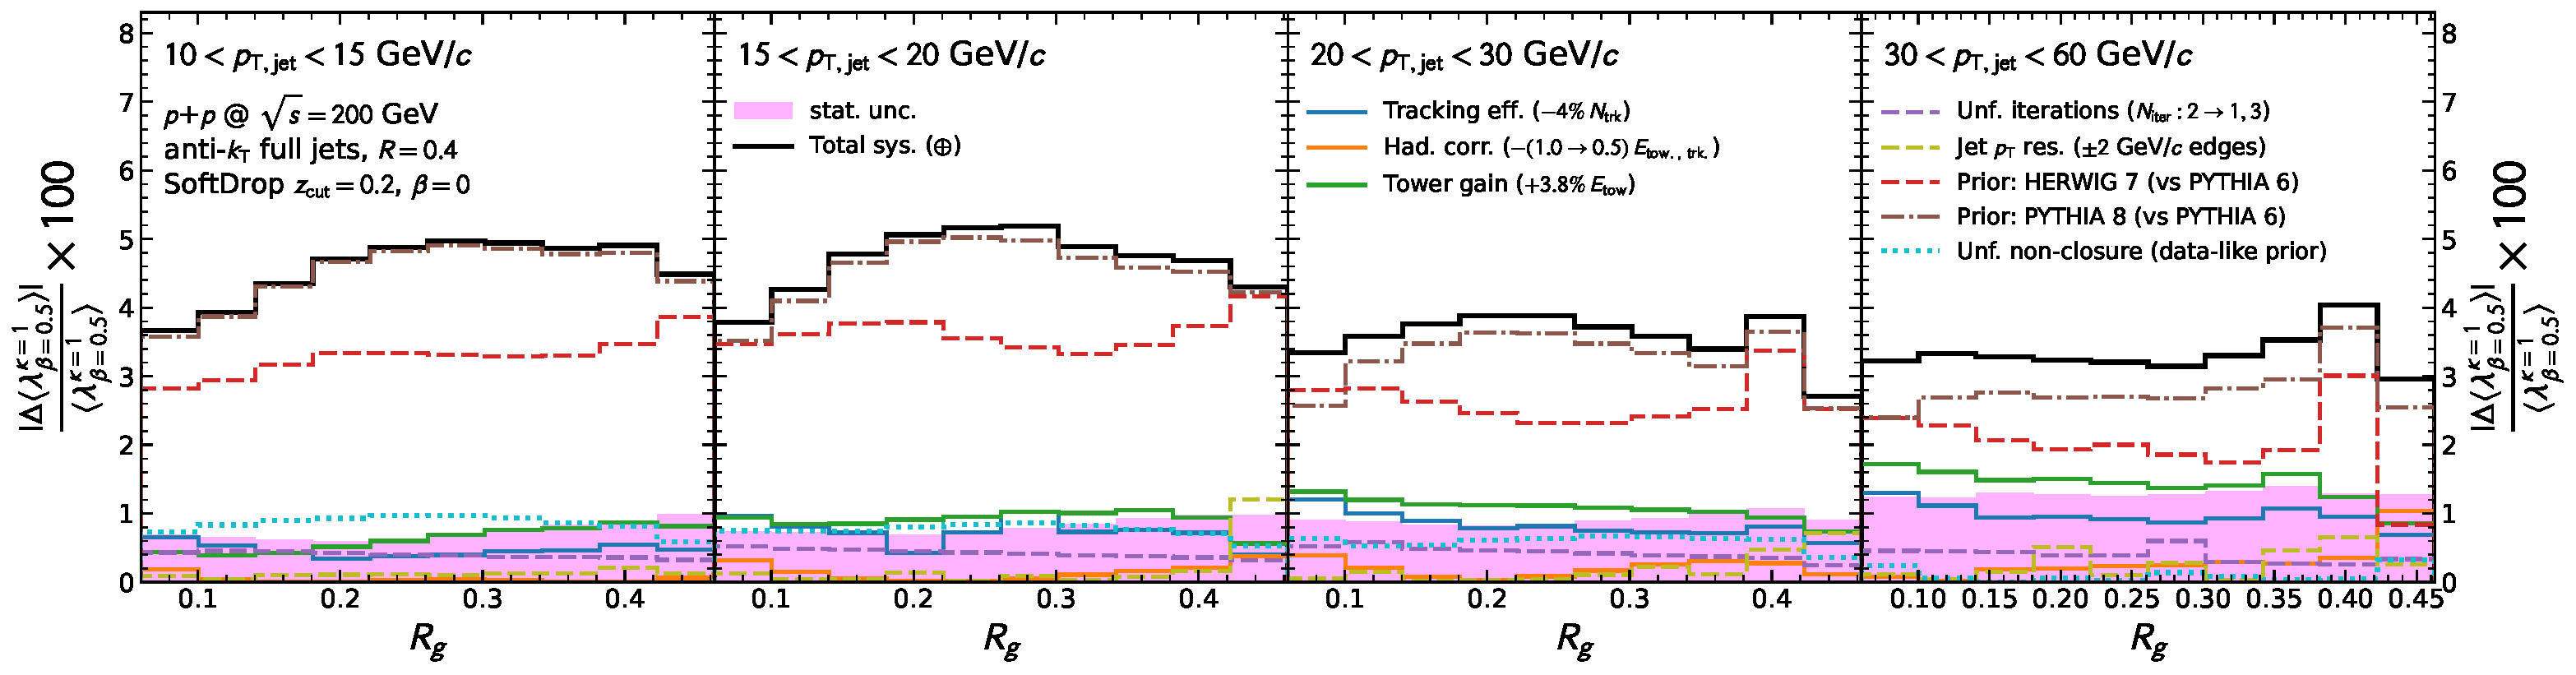
\includegraphics[width=\linewidth]{angularities/pp/sys_ch_ang_k1_b0.5_prof_incl_vs_sd_dR_raw.pdf}
	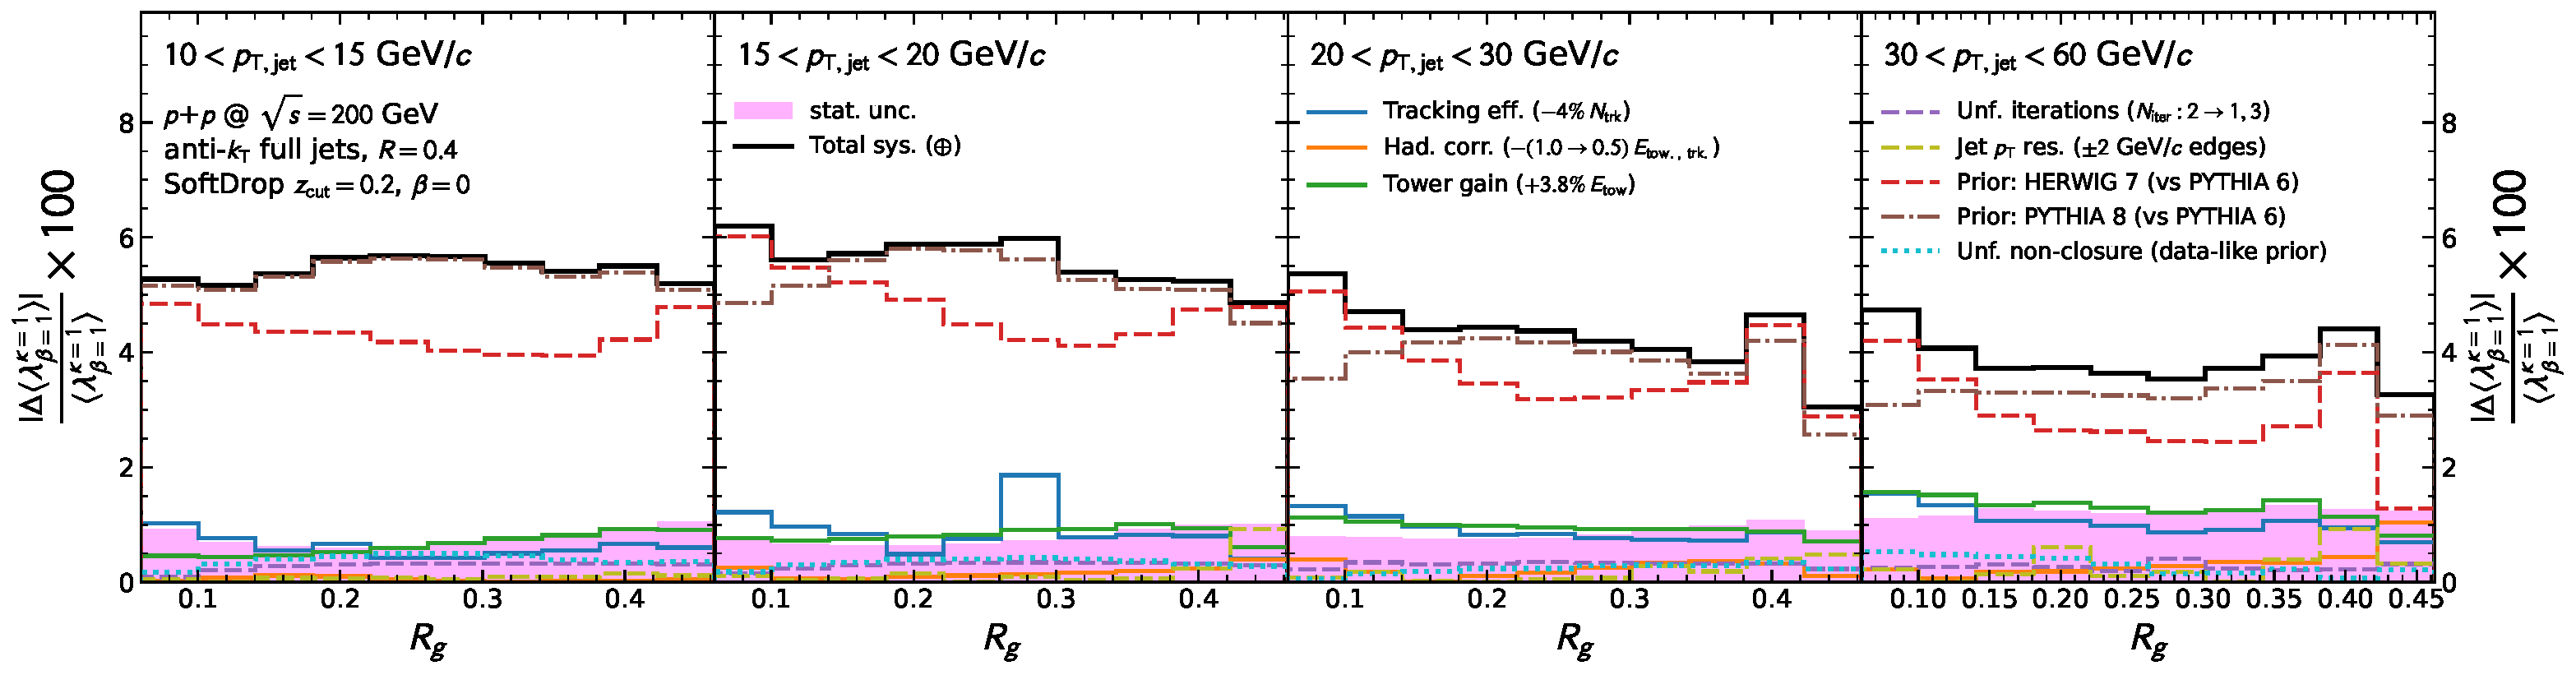
\includegraphics[width=\linewidth]{angularities/pp/sys_ch_ang_k1_b1_prof_incl_vs_sd_dR_raw.pdf}
	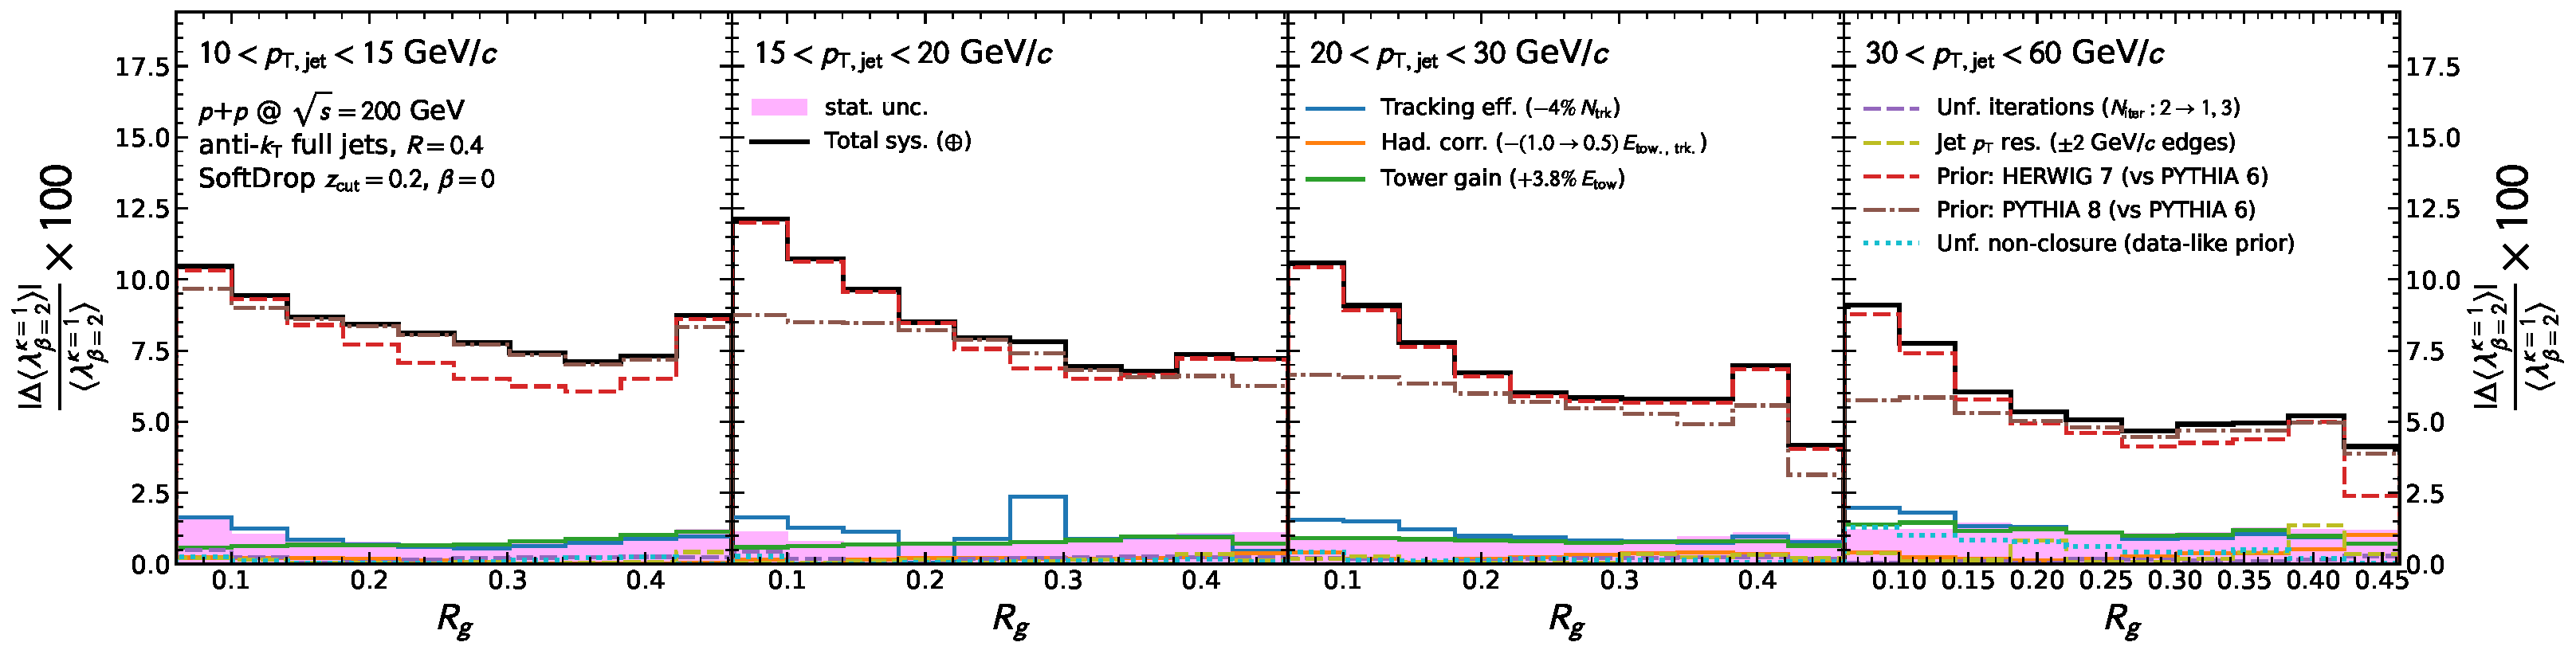
\includegraphics[width=\linewidth]{angularities/pp/sys_ch_ang_k1_b2_prof_incl_vs_sd_dR_raw.pdf}
	\caption{Relative systematic uncertainties of the \(\langle\lambda^{\kappa=1}_{\beta}\rangle\) vs.\ \(R_\mathrm{g}\) profiles of inclusive jets, before the Barlow check (Sec.~\ref{sec:barlow}), for \(\beta = 0.5\), 1 and 2 (top to bottom). The sources are the tracking efficiency, the hadronic correction and the tower gain (solid), the number of unfolding iterations, the jet-\(p_\mathrm{T}\) resolution and the HERWIG-7 and PYTHIA-8 priors (dashed), and the non-closure (dotted); the black line is their sum in quadrature and the magenta band is the statistical uncertainty. Jet-\(p_\mathrm{T}\) ranges are shown as panels.}
	\label{fig:SysProfInclRaw}
\end{figure}
\begin{figure}
	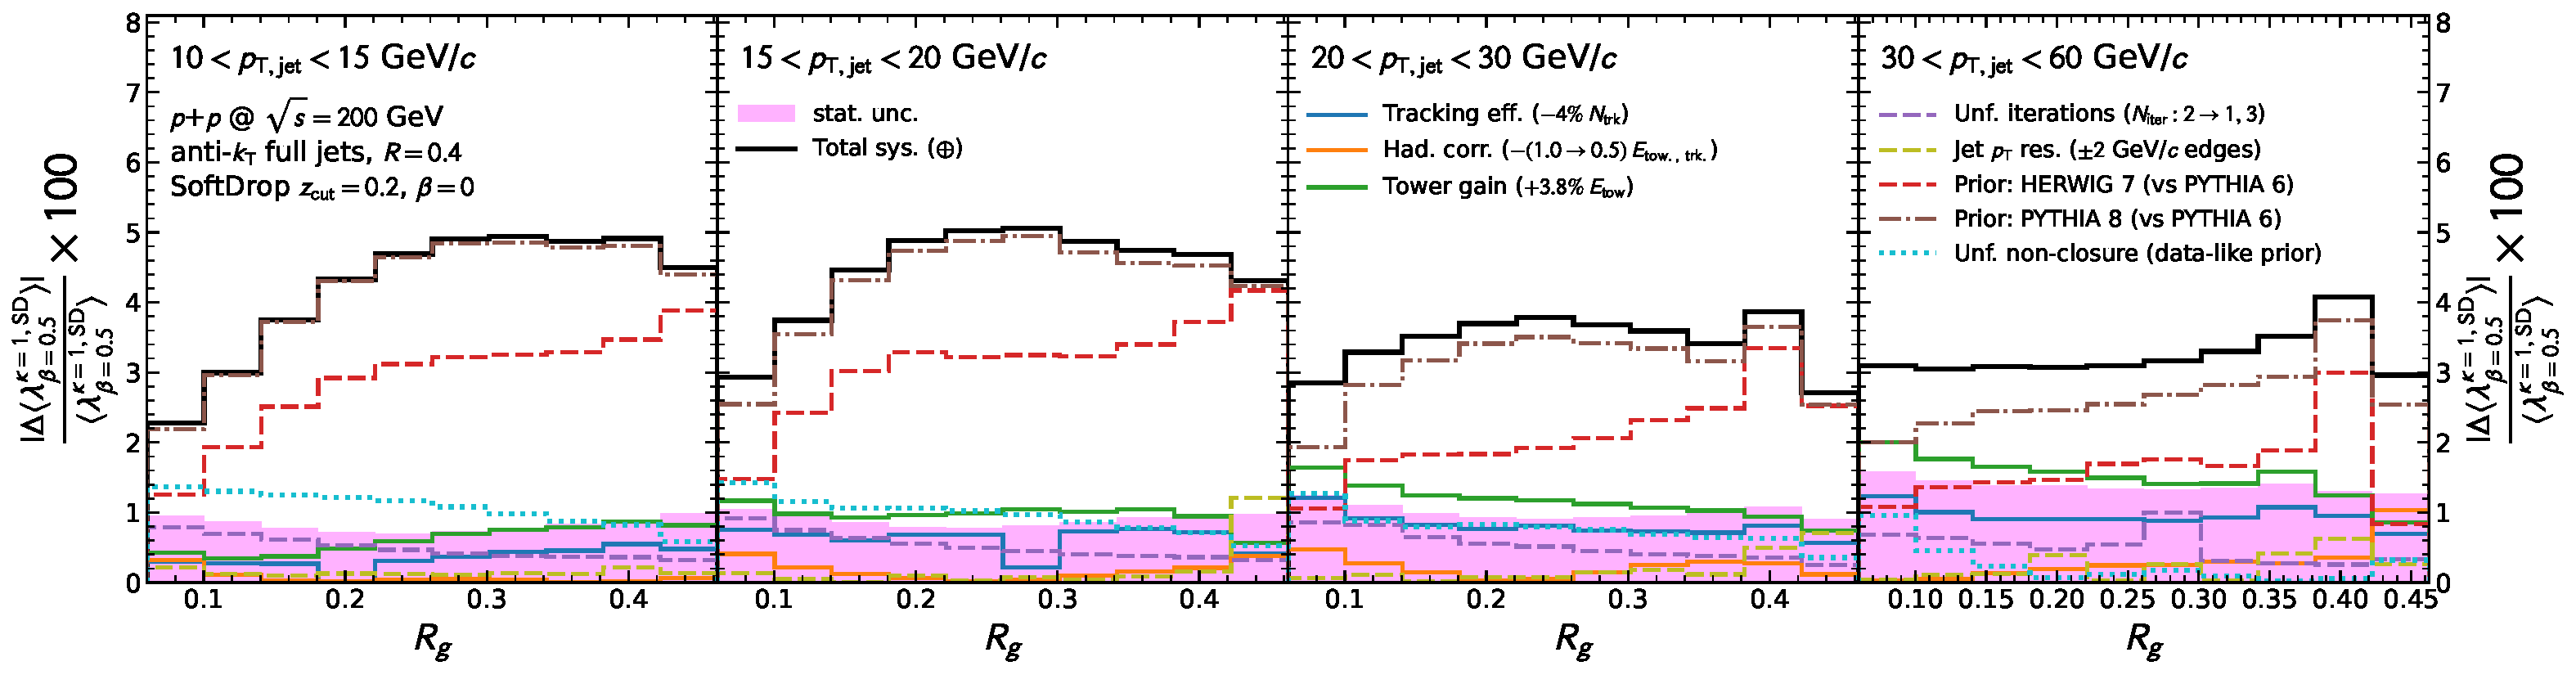
\includegraphics[width=\linewidth]{angularities/pp/sys_ch_ang_k1_b0.5_prof_sd_vs_sd_dR_raw.pdf}
	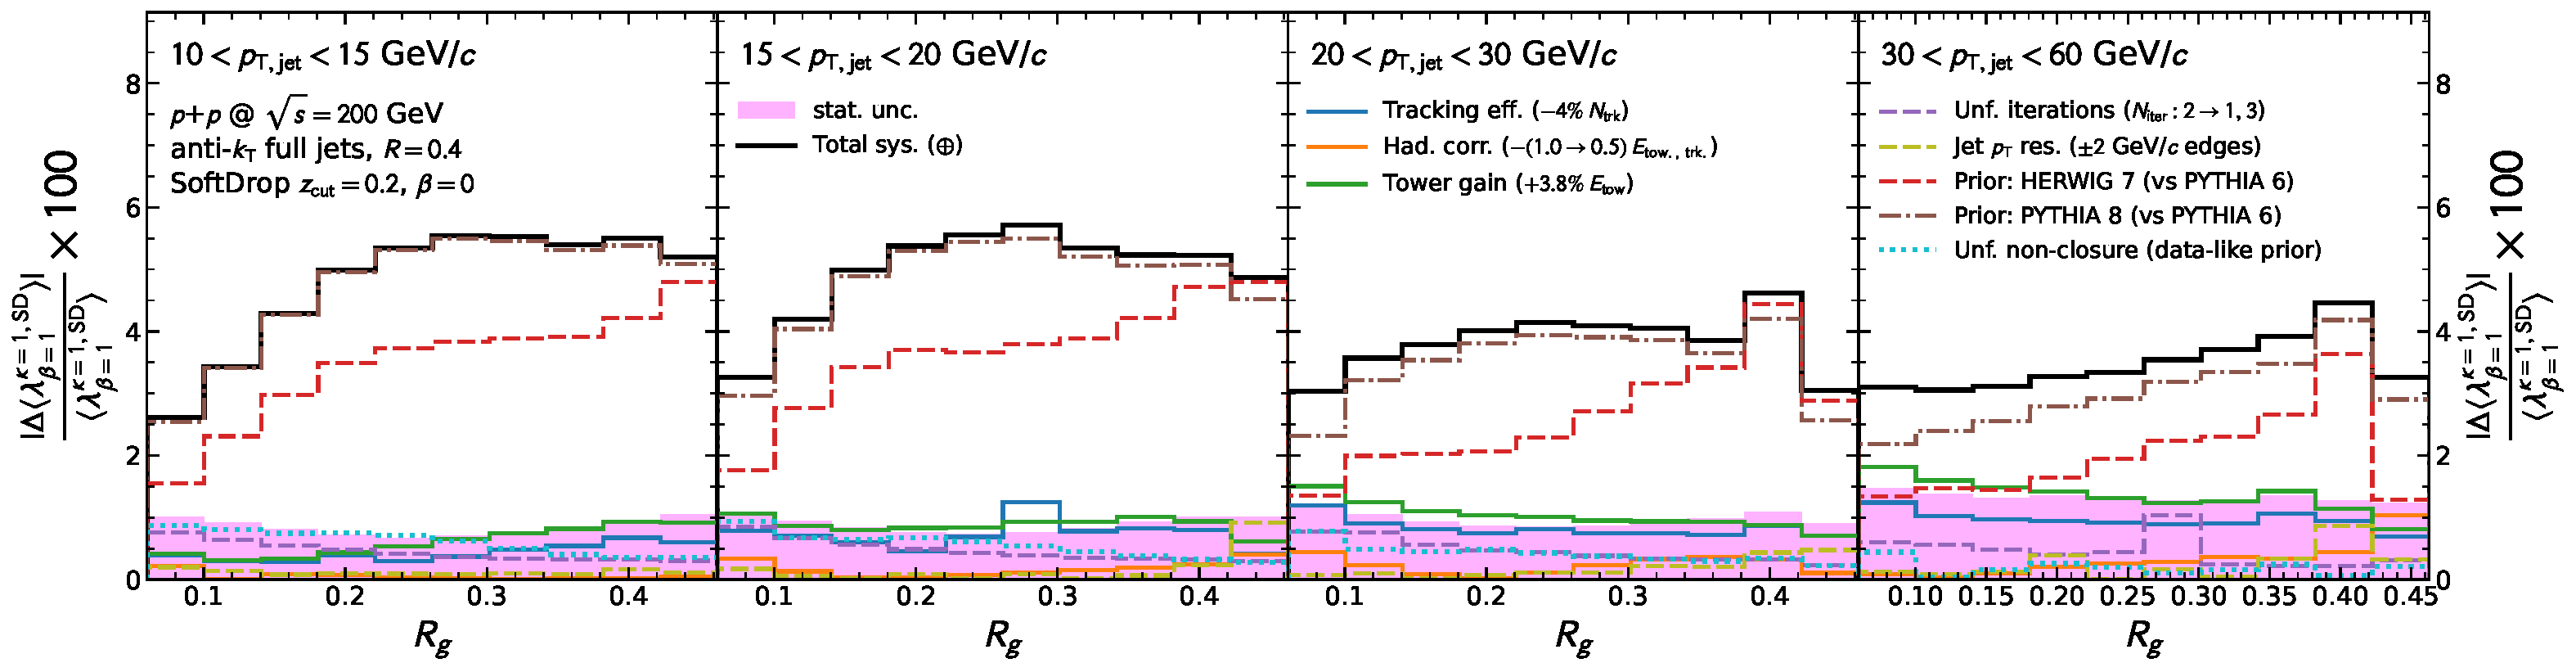
\includegraphics[width=\linewidth]{angularities/pp/sys_ch_ang_k1_b1_prof_sd_vs_sd_dR_raw.pdf}
	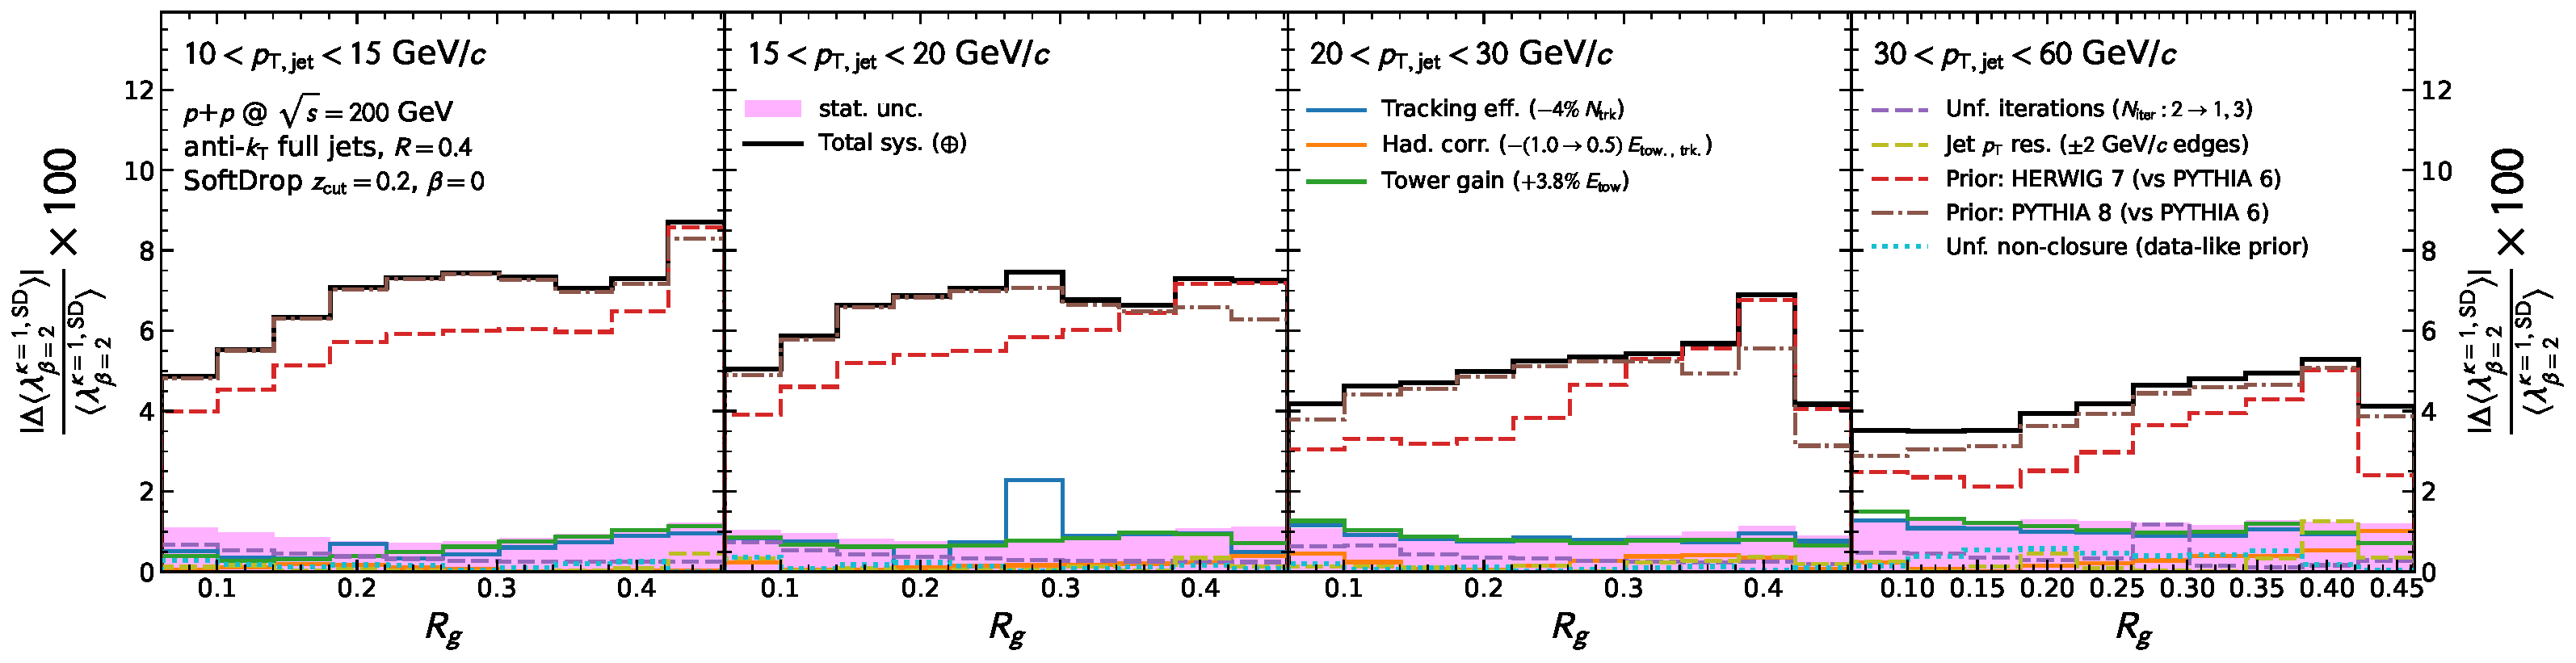
\includegraphics[width=\linewidth]{angularities/pp/sys_ch_ang_k1_b2_prof_sd_vs_sd_dR_raw.pdf}
	\caption{Relative systematic uncertainties of the \(\langle\lambda^{\kappa=1}_{\beta}\rangle\) vs.\ \(R_\mathrm{g}\) profiles of SoftDrop-groomed jets, before the Barlow check (Sec.~\ref{sec:barlow}), for \(\beta = 0.5\), 1 and 2 (top to bottom). The sources are the tracking efficiency, the hadronic correction and the tower gain (solid), the number of unfolding iterations, the jet-\(p_\mathrm{T}\) resolution and the HERWIG-7 and PYTHIA-8 priors (dashed), and the non-closure (dotted); the black line is their sum in quadrature and the magenta band is the statistical uncertainty. Jet-\(p_\mathrm{T}\) ranges are shown as panels.}
	\label{fig:SysProfSDRaw}
\end{figure}

 \begin{itemize}
 	\item Tracking Efficiency -  The uncertainty in tracking efficiency (Sect.~\ref{sec:TrackTowerSel}) is estimated at $\pm 4 \%$ for \(p+p\) events.
 	\item Variation of Hadronic Correction - For the towers, we remove the full contribution of the track momentum for our central values (Eq.~\ref{Eq:HadCorr}, \(f_\mathrm{had} = 1\)). As a variation on that, we remove half of the total track momentum contribution.
 	\item Tower Gain Uncertainty - Tower energies increased by 3.8\%
 	\item \(p_\mathrm{T, jet}\) resolution - Use the \(p_\mathrm{T, jet}\) resolution values from fig.~\ref{fig:PtResolution} to shift the \(p_\mathrm{T, jet}\) windows in which results are presented. 
 \end{itemize}
 
 \subsubsection{Unfolding related uncertainties}
 \begin{itemize}
 	\item Variation of the regularization parameter(number of iterations) -  For our central values, we have used 2 iterations as we found the result to converge reliably by that point. The number of iterations is varied to 1 and 3.
 	\item Prior variation - Varied the prior of the embedding sample from PYTHIA6 to HERWIG7 and to PYTHIA8 by reweighting (Sec.~\ref{sec:priorReweighting})
 	\item Non Closure - Any deviations from 1 for ratios shown in fig.~\ref{fig:ClosureAngularity} and fig.~\ref{fig:ClosureAngVsRg}, with the data-like prior of Sec.~\ref{sec:priorReweighting}
 \end{itemize}

 \subsubsection{Prior reweighting}
 \label{sec:priorReweighting}
 The prior of the unfolding is the generated distribution of the embedding simulation, \(p_{\mathrm{gen.}, 0}(\mathbf{x})\), together with the reconstructed distribution \(p_{\mathrm{reco.}, 0}(\mathbf{y})\) it produces through the response \(R(\mathbf{y}, \mathbf{x})\).
 %
 Two kinds of alternative priors are used: the particle-level distributions of HERWIG7 and PYTHIA8, for the prior variation, and a data-like PYTHIA6 prior, which provides the pseudo-data of the closure test.
 %
 Neither is obtained by a new detector simulation.
 %
 Instead, the PYTHIA6 embedding jets are reweighted, which changes the prior while keeping the PYTHIA6+GEANT3 response \(R(\mathbf{y}, \mathbf{x})\) fixed, so that each variation probes the dependence on the prior alone.

 Each reweighting is a density ratio learned with a classifier, in the same way as \(\omega\) and \(\nu\) in the unfolding.
 %
 A classifier \(f\) trained with the binary cross-entropy to separate a target sample (label 1) from the PYTHIA6 sample (label 0) gives the per-jet weight
 \begin{equation}
 	\label{eq:priorRatio}
 	r(\mathbf{x}) = \frac{1}{C}\,\frac{f(\mathbf{x})}{1 - f(\mathbf{x})} \approx \frac{p_\mathrm{target}(\mathbf{x})}{p_\mathrm{PYTHIA6}(\mathbf{x})} ,
 \end{equation}
 over the full joint feature vector, so that correlations between the observables are reweighted along with their one-dimensional distributions.
 %
 The classifier has the architecture and optimizer of the unfolding classifiers, and the jets carry their \(\hat{p}_\mathrm{T}\) cross-section weights, with the target normalized to the total weight of the PYTHIA6 sample.
 %
 Since the jet spectrum falls steeply, the loss would be dominated by the lowest-\(p_\mathrm{T, jet}\) jets.
 %
 Both classes are therefore given the common training weight \(c(p_\mathrm{T, jet}) = [p_\mathrm{PYTHIA6}(p_\mathrm{T, jet})]^{-1/2}\), with \(p_\mathrm{PYTHIA6}(p_\mathrm{T, jet})\) the weighted jet-\(p_\mathrm{T}\) density of the PYTHIA6 sample.
 %
 Being a function of a feature shared by both classes, \(c\) cancels in eq.~\ref{eq:priorRatio} and only shifts the training towards higher \(p_\mathrm{T, jet}\).
 %
 An ensemble of 10 classifiers is trained; their odds are clamped to \([0.1, 10]\) and combined by the geometric mean.
 %
 The constant \(C\) normalizes the weighted mean of \(r\) over the PYTHIA6 sample to one, so that only the shape of the prior changes and not its total cross-section.

 \paragraph{Generator priors.} The targets are the HERWIG7 and PYTHIA8 particle-level jets, selected with the particle-level cuts of the embedding (\ptGeq{jet}{5}, \(|\eta_\mathrm{jet}| < 0.6\), at least two charged constituents) and described by the same features.
 %
 The weight \(r(\mathbf{x})\) is evaluated on every generated PYTHIA6 jet, matched or missed, and each matched reconstructed jet inherits the weight of its generated partner; fakes, having no generated partner, are unchanged.
 %
 The reweighted embedding replaces the nominal one in the full unfolding, and the difference of the result to the nominal one is taken as the uncertainty of each generator, entering the envelope of the unfolding uncertainties.
%
The reweighted PYTHIA-6 jets are compared to their HERWIG-7 and PYTHIA-8 targets in Figs.~\ref{fig:reweight_herwig7} and \ref{fig:reweight_pythia8}: the reweighting reproduces the target distributions and \(\langle\lambda^{\kappa=1}_{\beta}\rangle\) vs.\ \(R_\mathrm{g}\) profiles to within a few percent in most bins, including the differences in their correlation with \(R_\mathrm{g}\), which a reweighting of one-dimensional distributions would not capture.
  \begin{sidewaysfigure}
 	\begin{tabularx}{\textwidth}{XX}
 		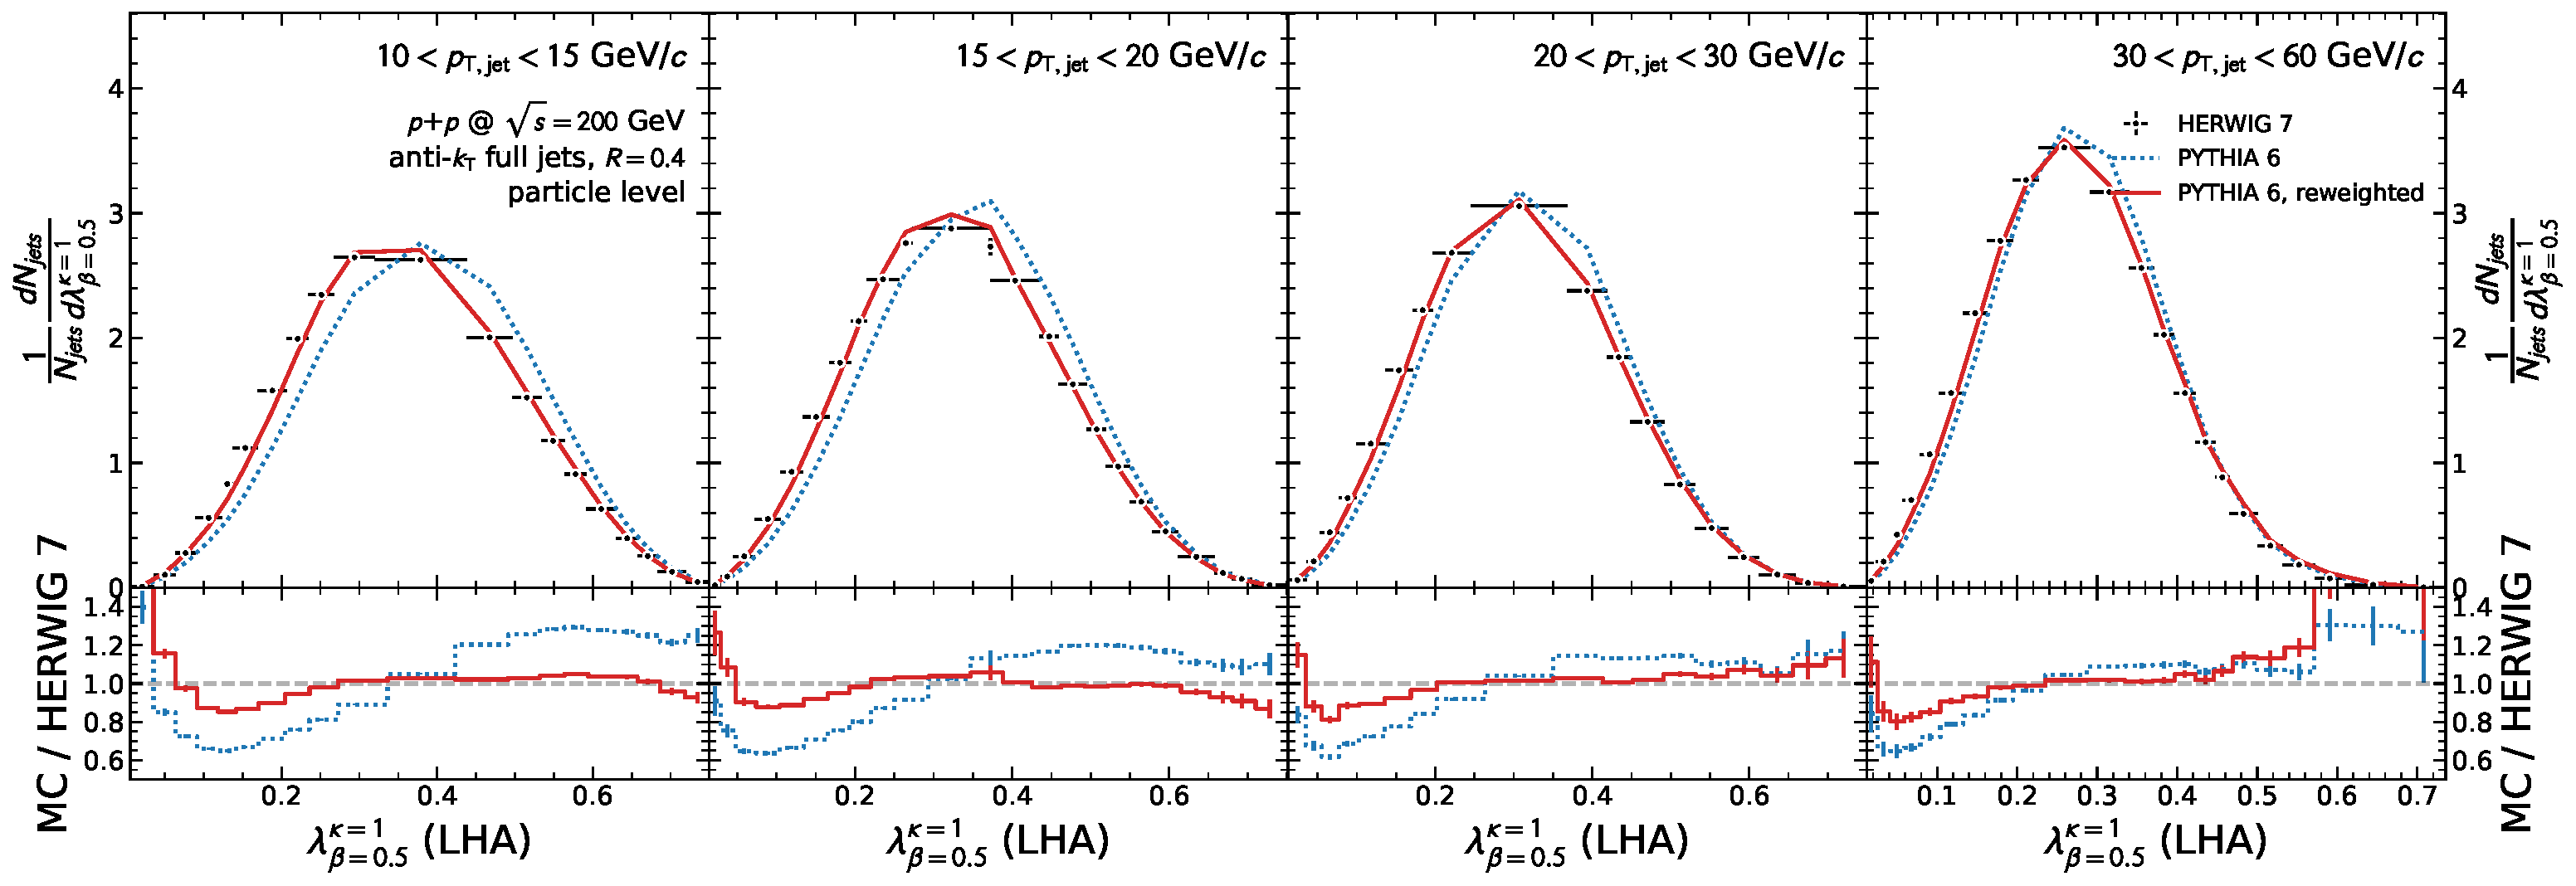
\includegraphics[width=\linewidth]{figures/angularities/pp/reweight_herwig7_ch_ang_k1_b0.5.pdf}&
 		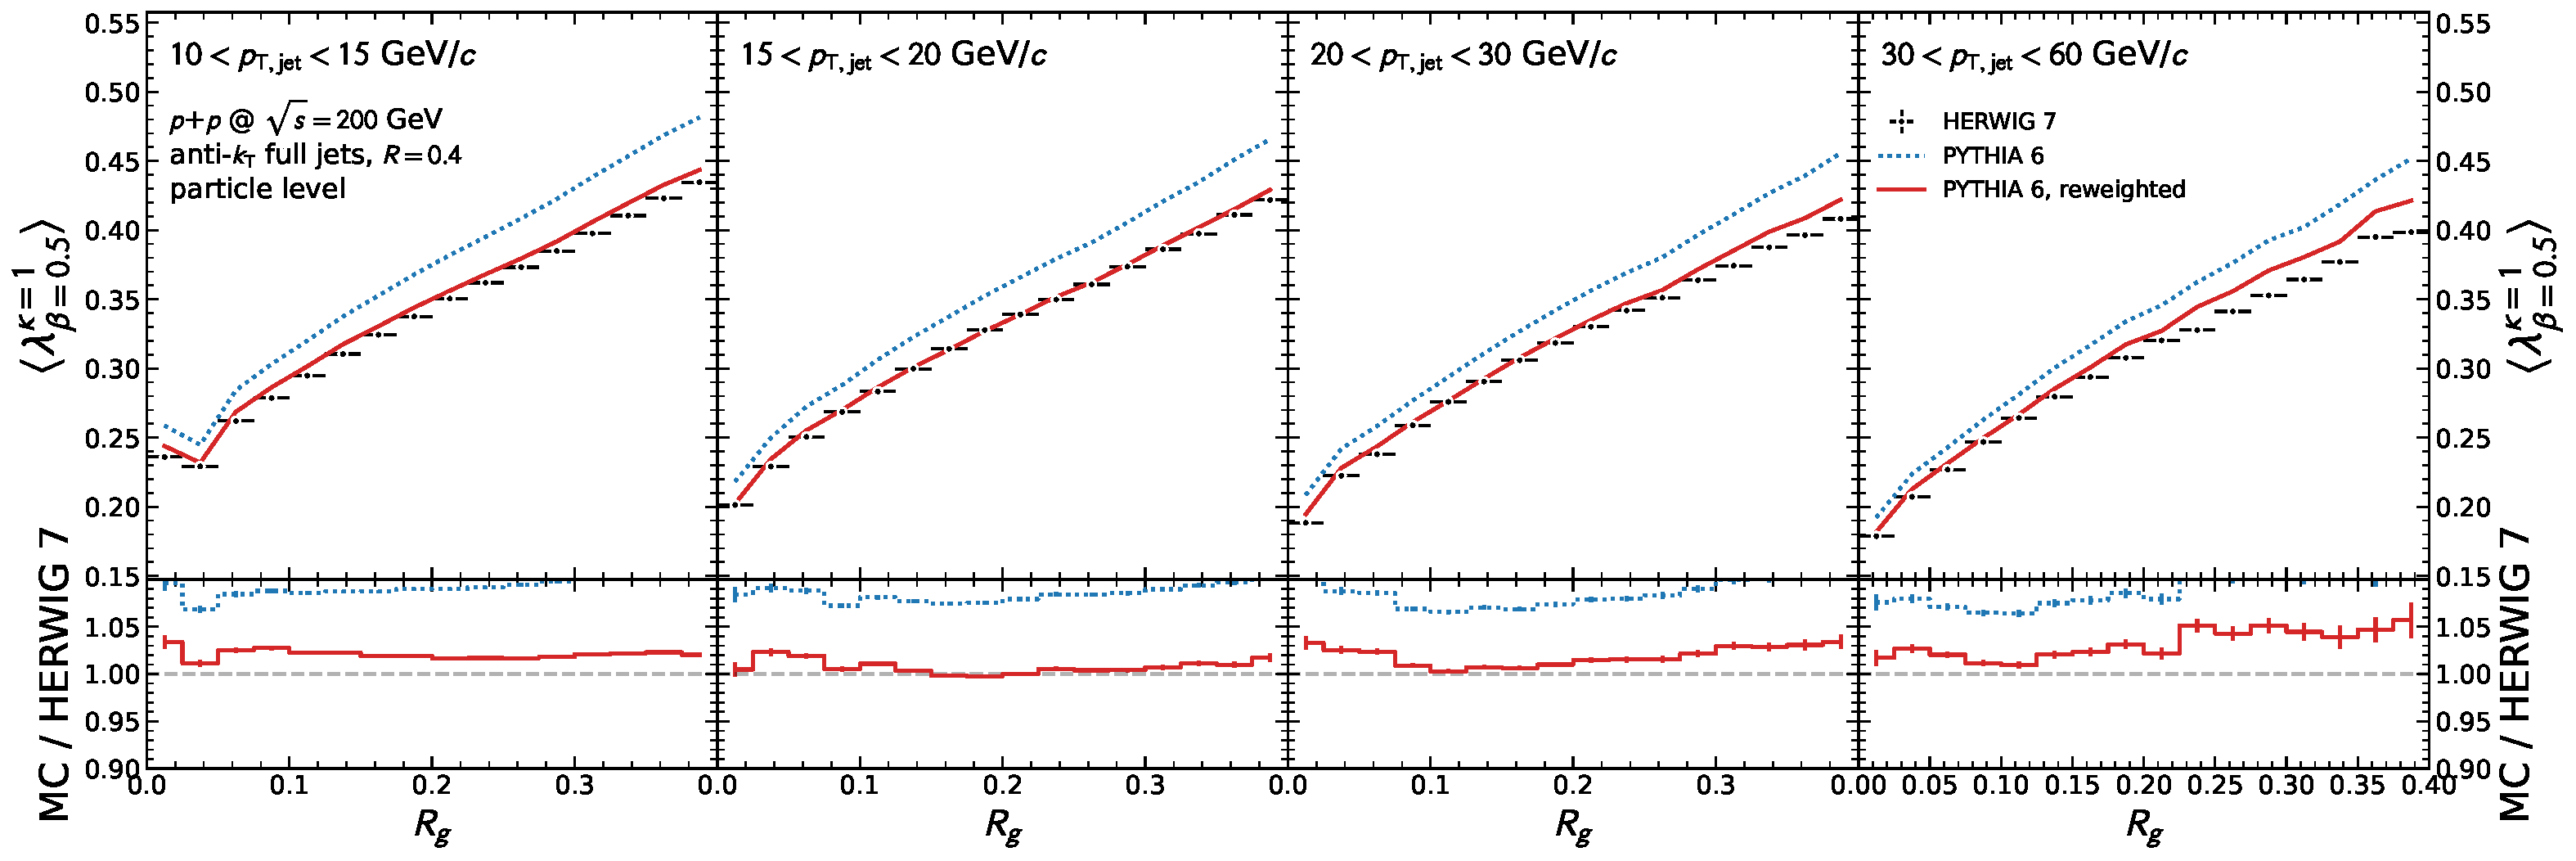
\includegraphics[width=\linewidth]{figures/angularities/pp/reweight_herwig7_prof_ch_ang_k1_b0.5.pdf}\\
 		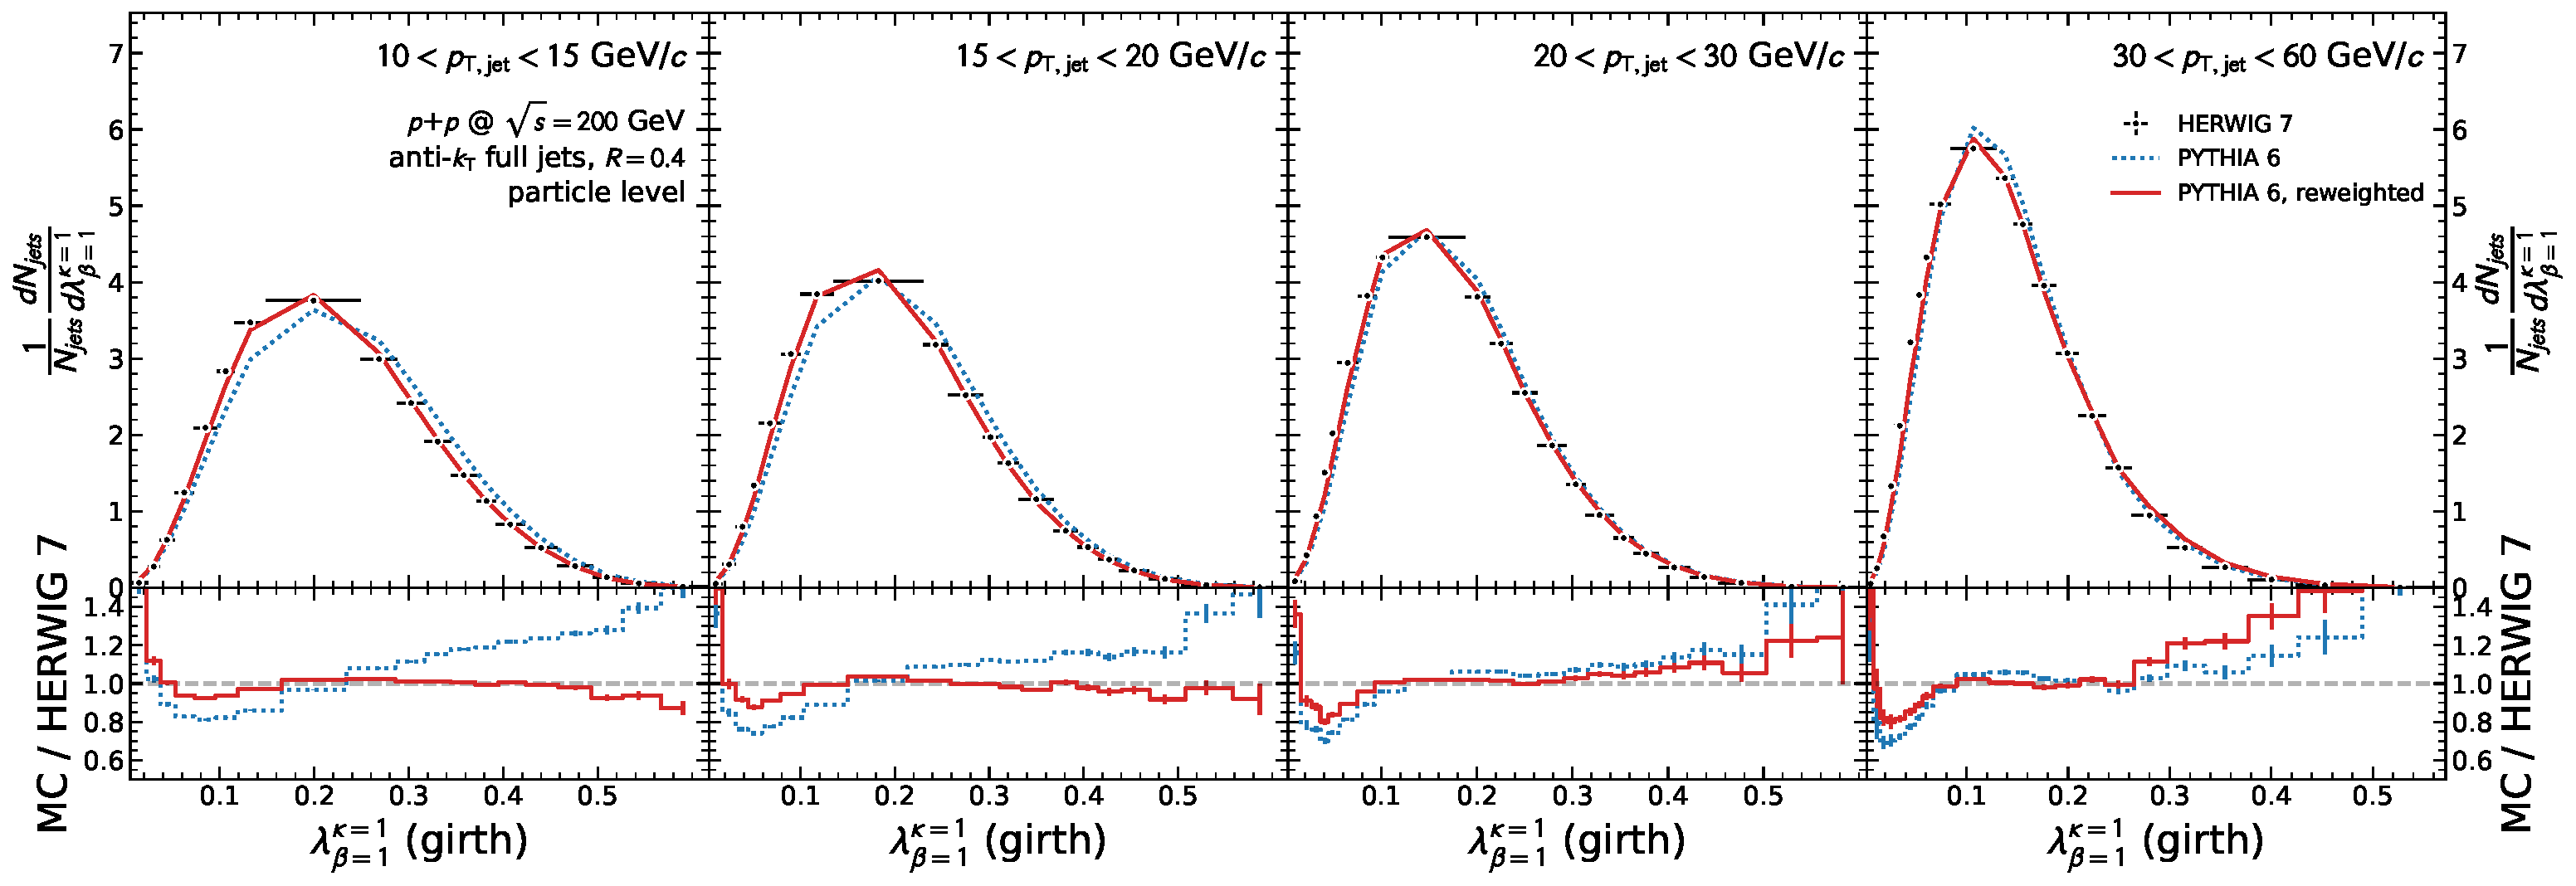
\includegraphics[width=\linewidth]{figures/angularities/pp/reweight_herwig7_ch_ang_k1_b1.pdf}&
 		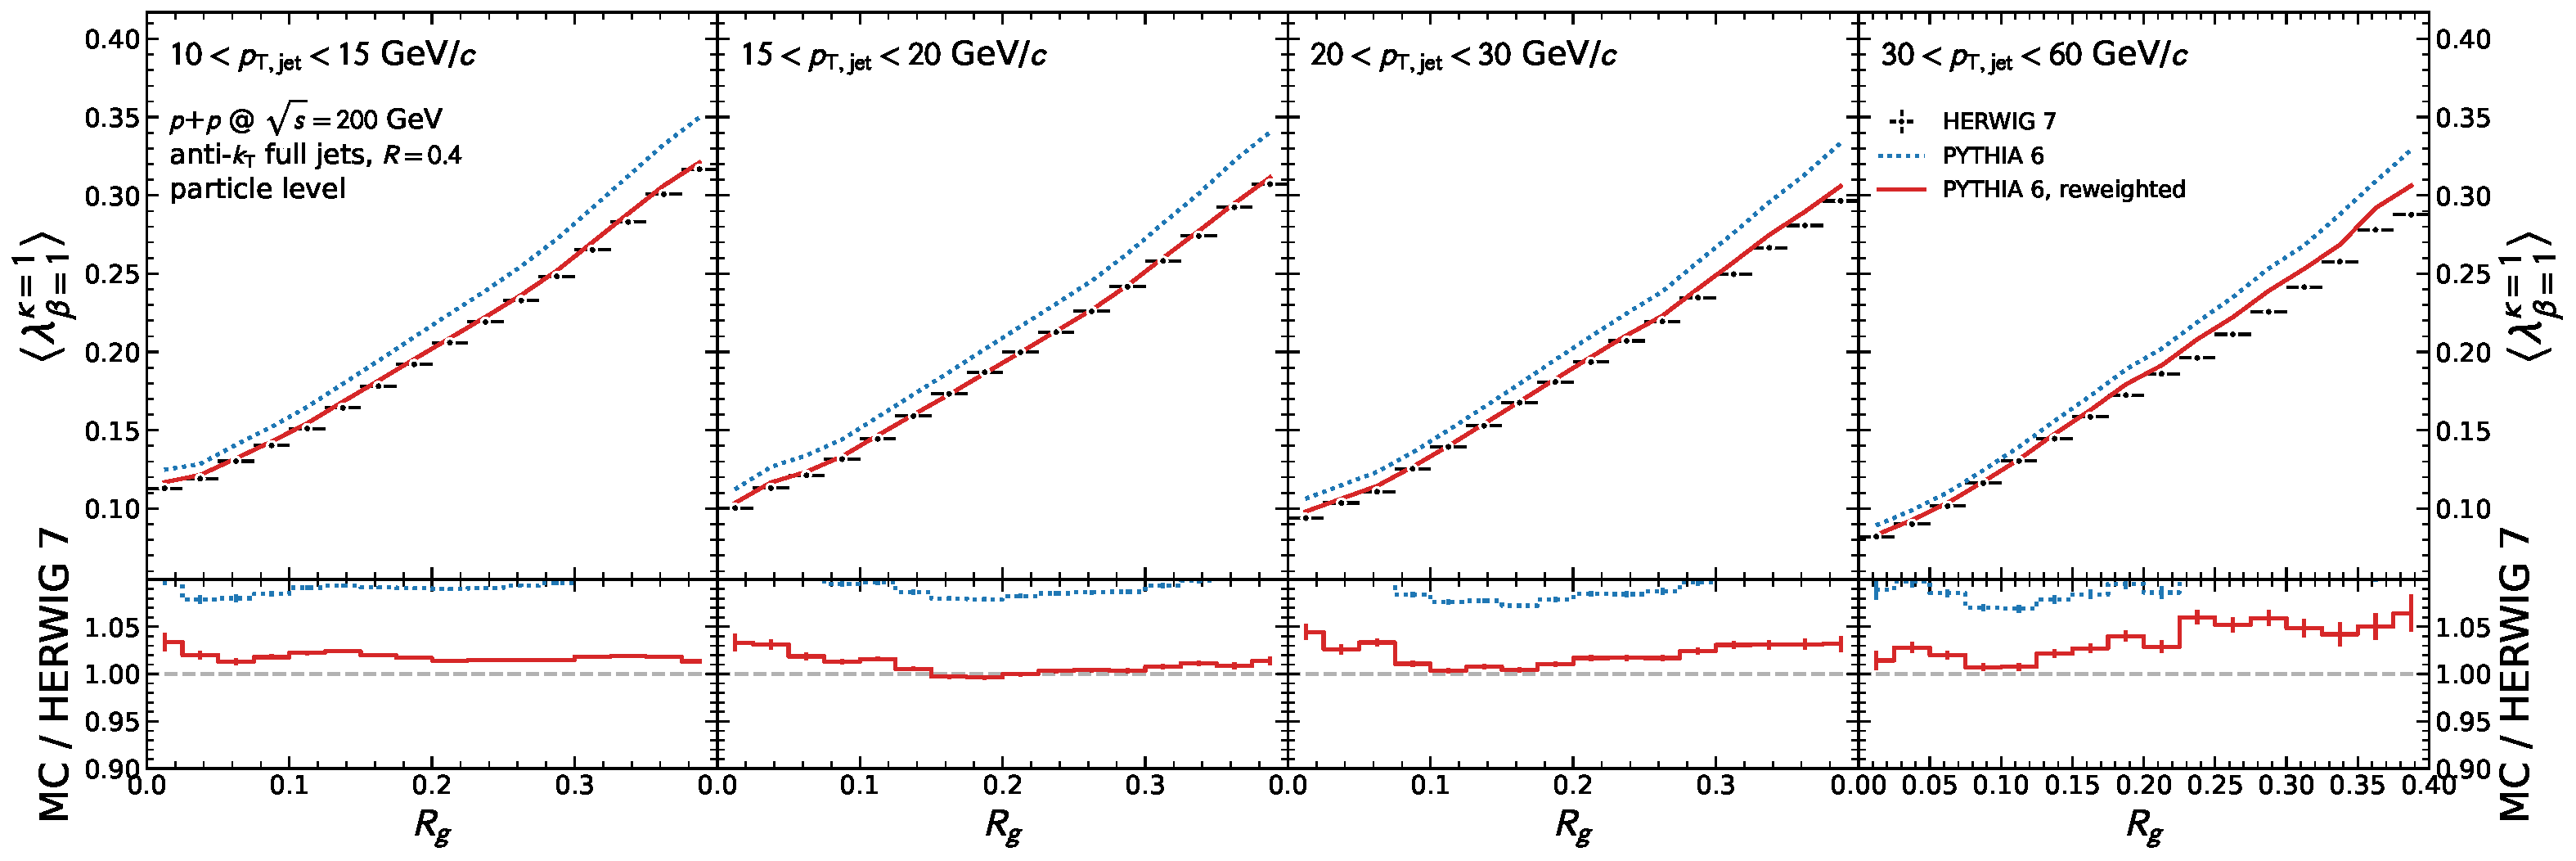
\includegraphics[width=\linewidth]{figures/angularities/pp/reweight_herwig7_prof_ch_ang_k1_b1.pdf}\\
 		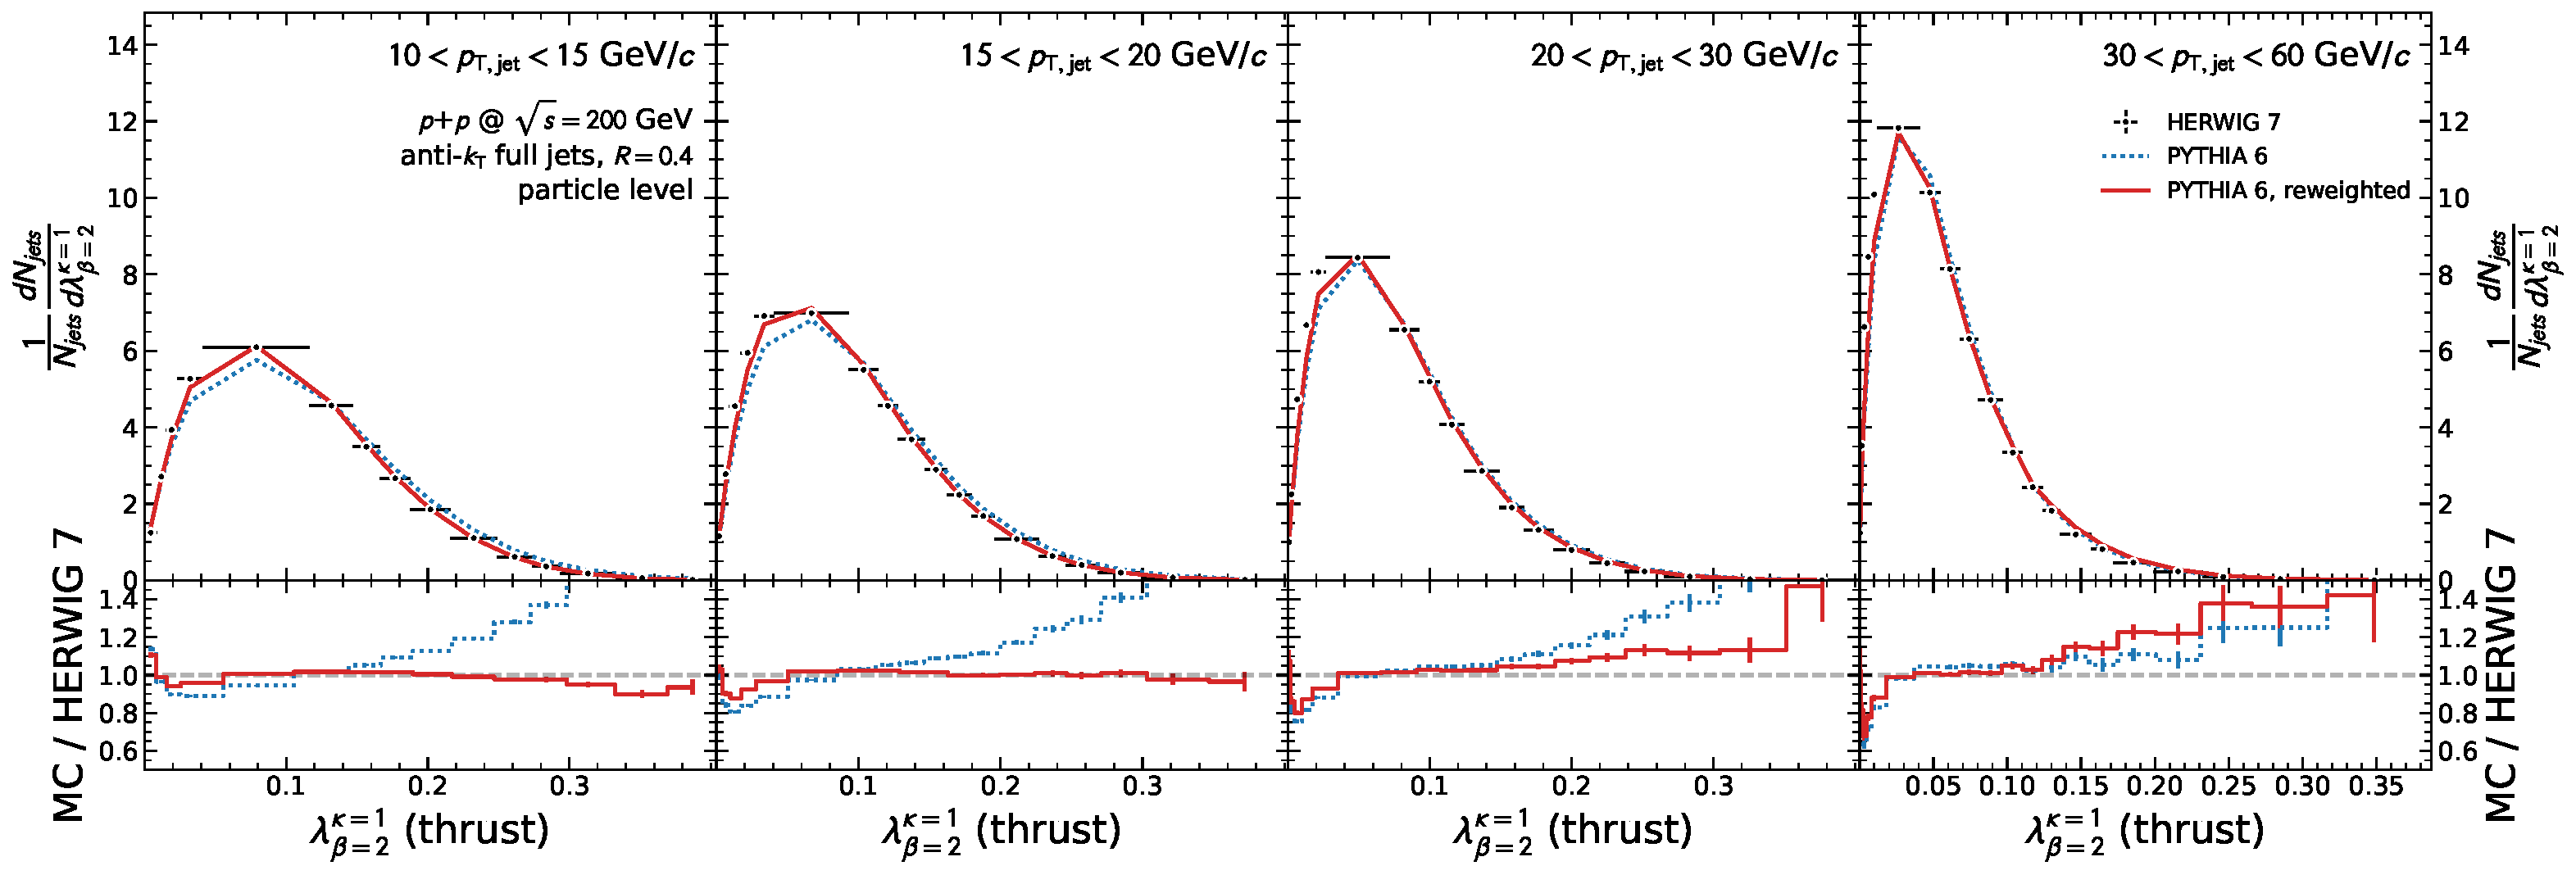
\includegraphics[width=\linewidth]{figures/angularities/pp/reweight_herwig7_ch_ang_k1_b2.pdf}&
 		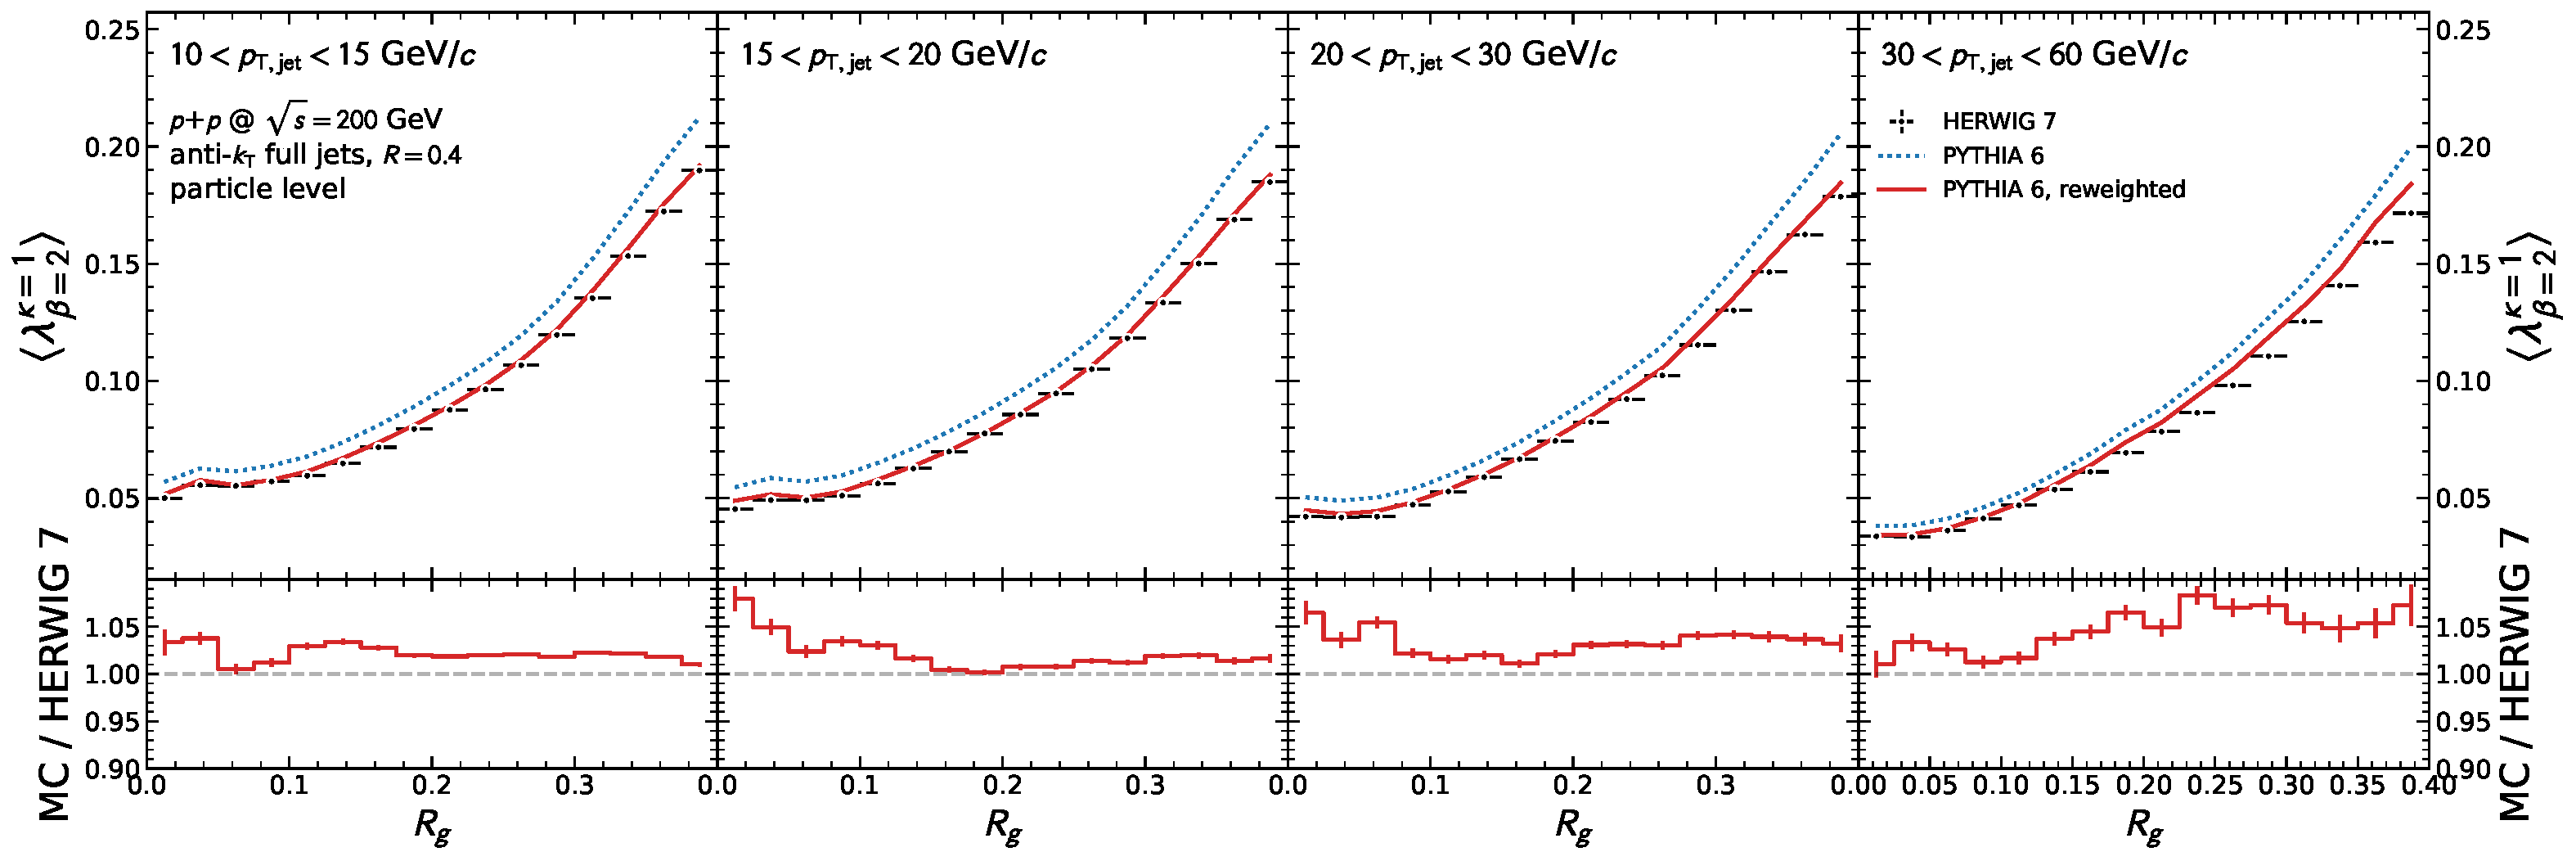
\includegraphics[width=\linewidth]{figures/angularities/pp/reweight_herwig7_prof_ch_ang_k1_b2.pdf}
 	\end{tabularx}
 	\caption{Reweighting of the PYTHIA-6 prior to HERWIG-7 at particle level: the distributions of \(\lambda^{\kappa=1}_{\beta}\) (left) and the \(\langle\lambda^{\kappa=1}_{\beta}\rangle\) vs.\ \(R_\mathrm{g}\) profiles (right) for \(\beta = 0.5\), 1 and 2 (top to bottom), in four \(p_\mathrm{T, jet}\) ranges (panels). HERWIG-7 (points) is compared to the nominal (dotted) and the reweighted (solid) PYTHIA-6; the lower panels show their ratios to HERWIG-7.}
 	\label{fig:reweight_herwig7}
 \end{sidewaysfigure}
 
  \begin{sidewaysfigure}
 	\begin{tabularx}{\textwidth}{XX}
 		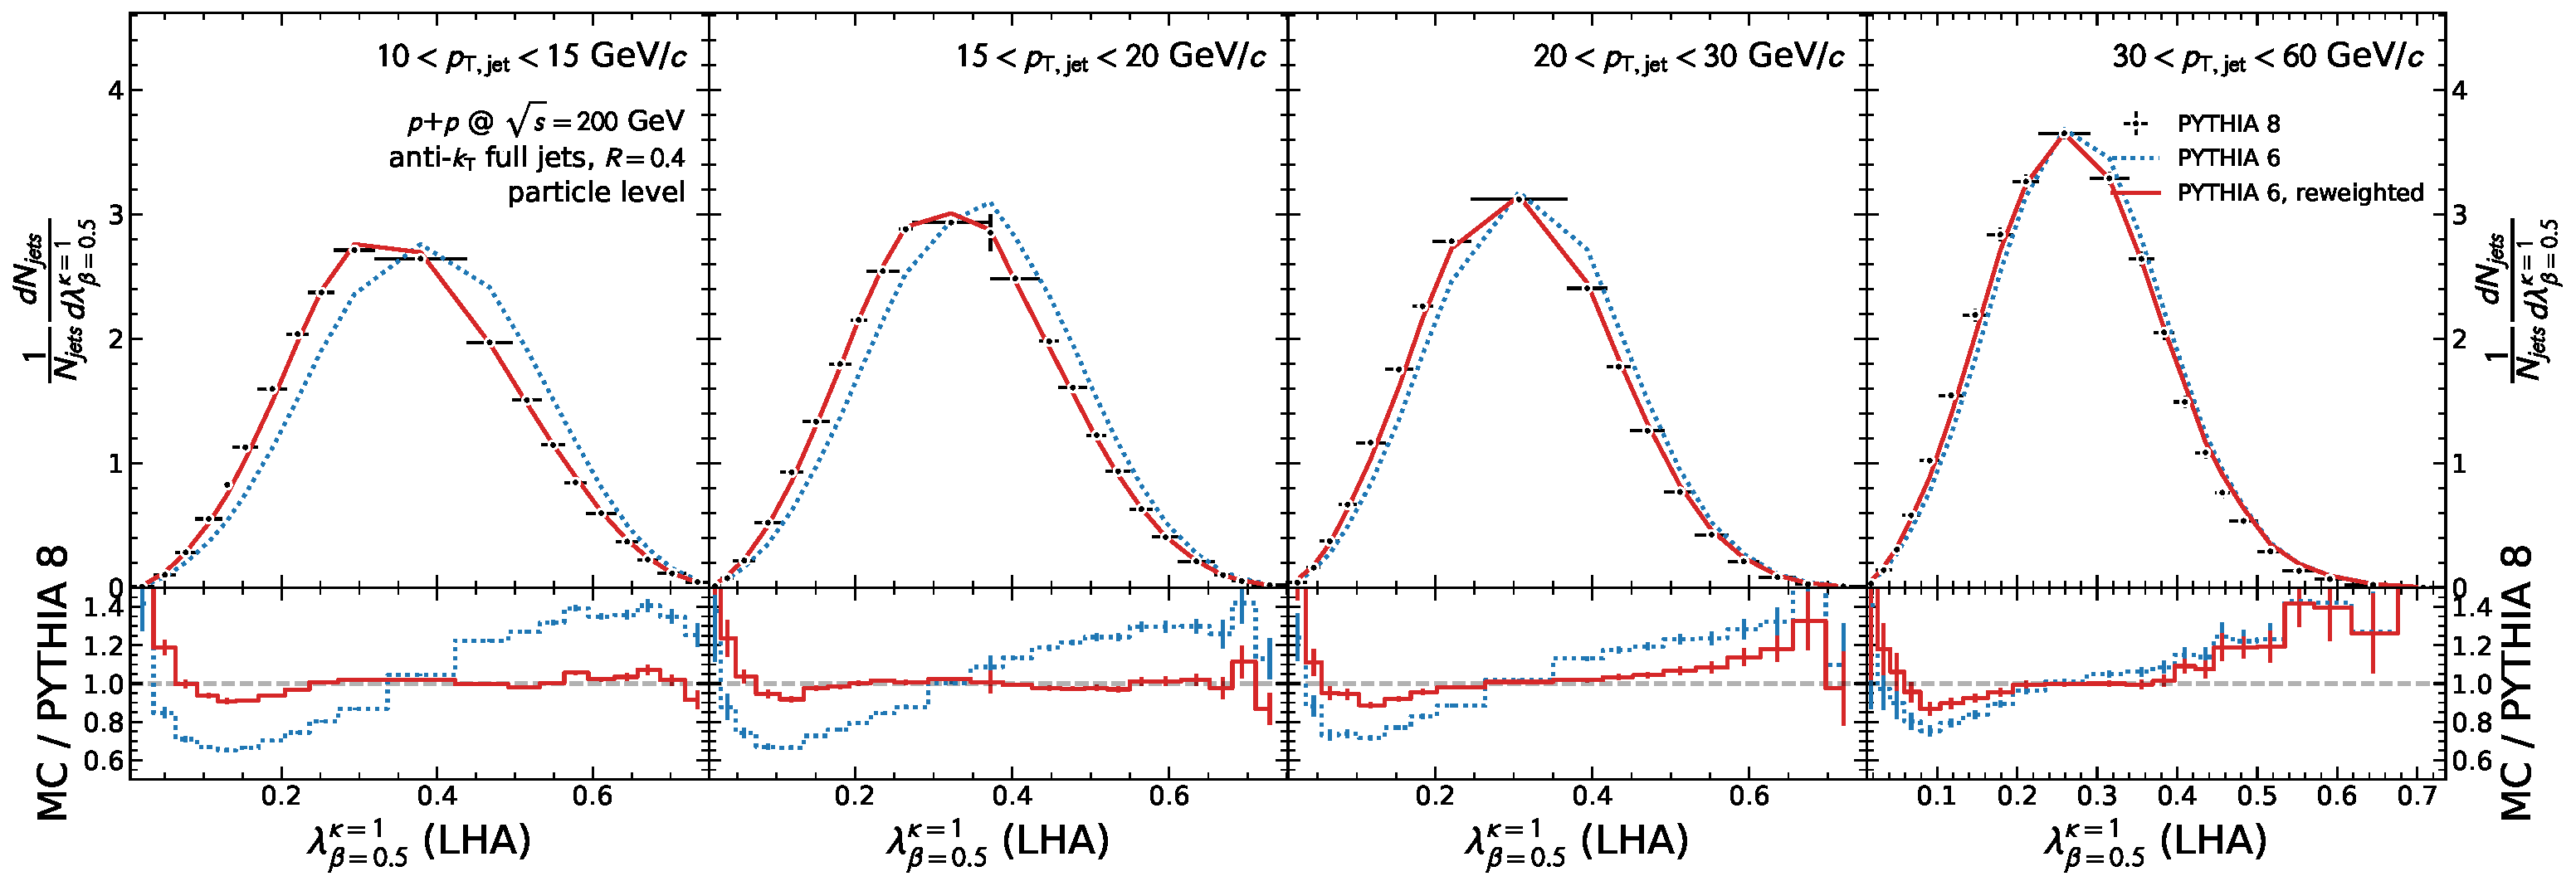
\includegraphics[width=\linewidth]{figures/angularities/pp/reweight_pythia8_ch_ang_k1_b0.5.pdf}&
 		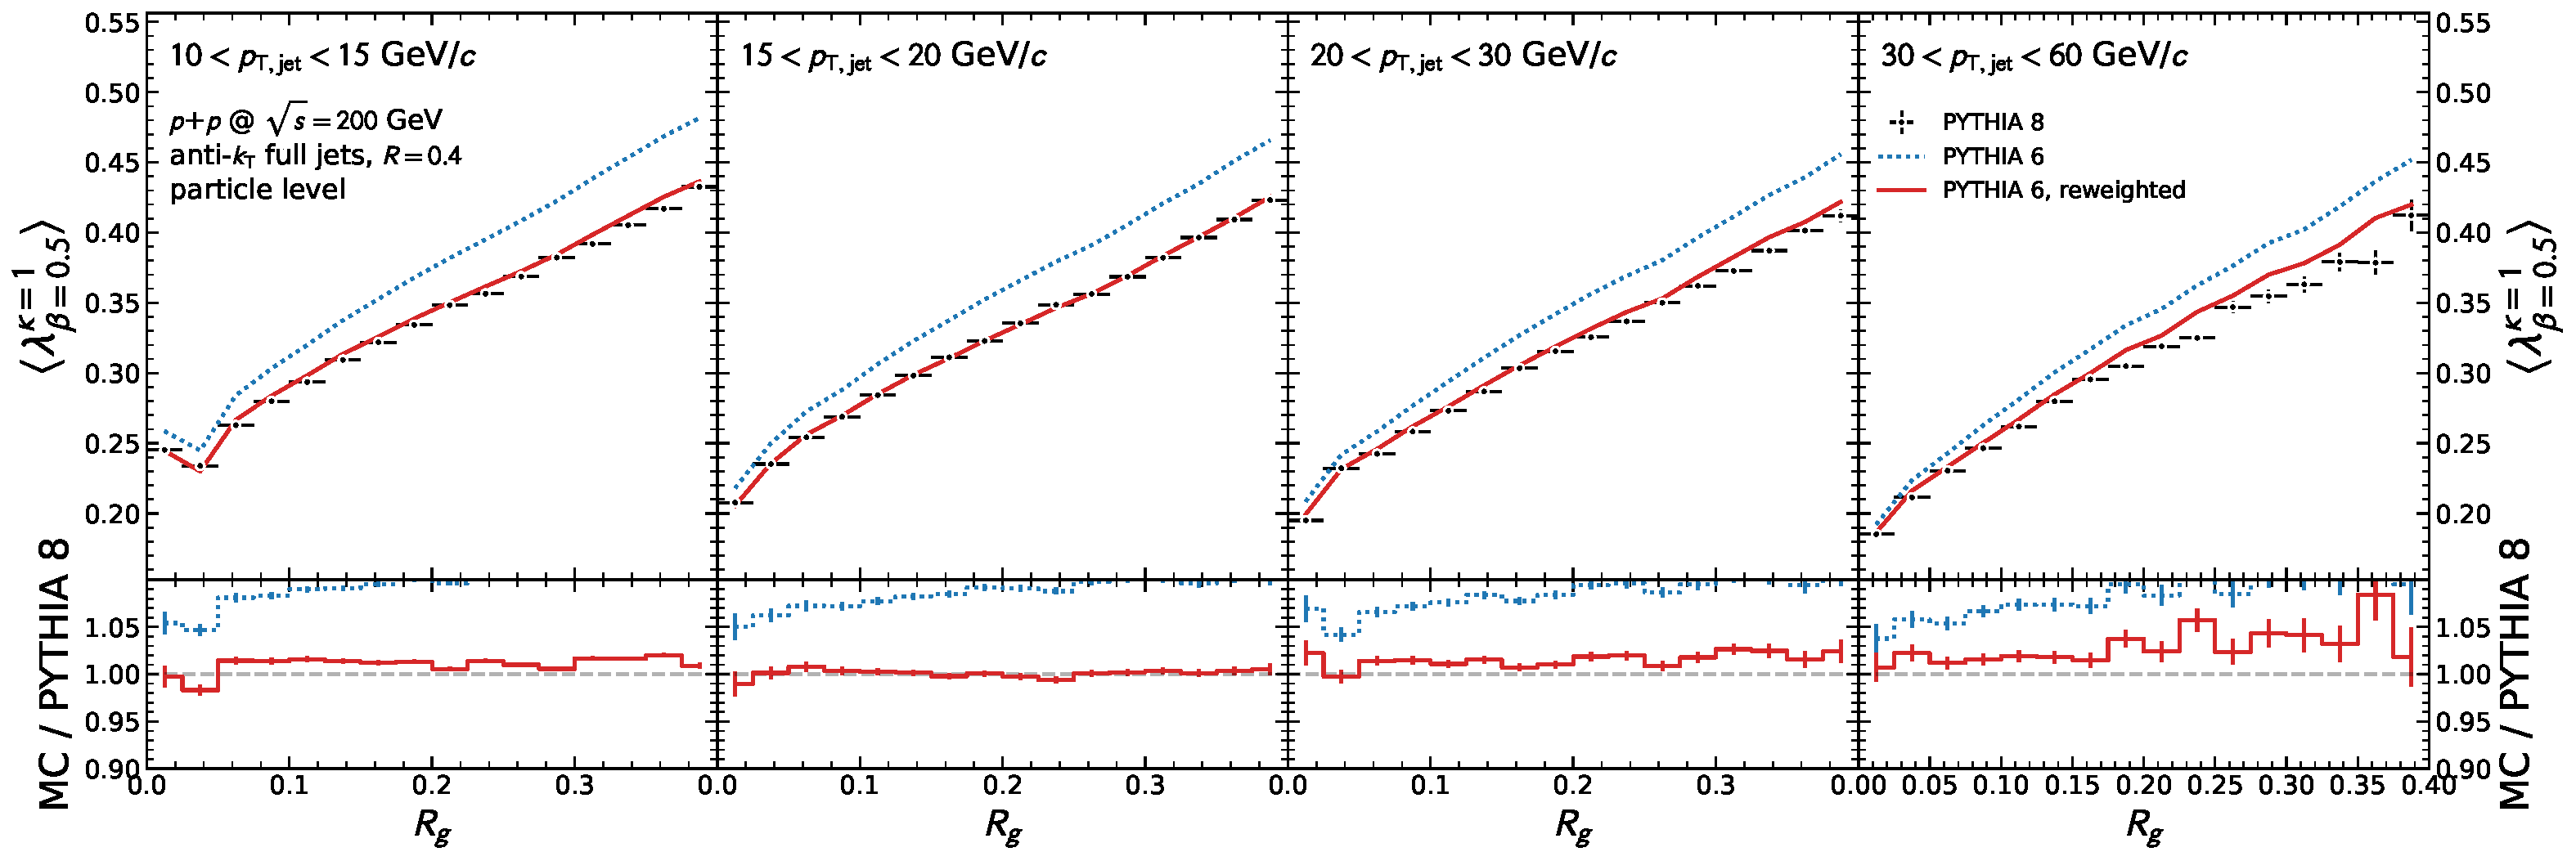
\includegraphics[width=\linewidth]{figures/angularities/pp/reweight_pythia8_prof_ch_ang_k1_b0.5.pdf}\\
 		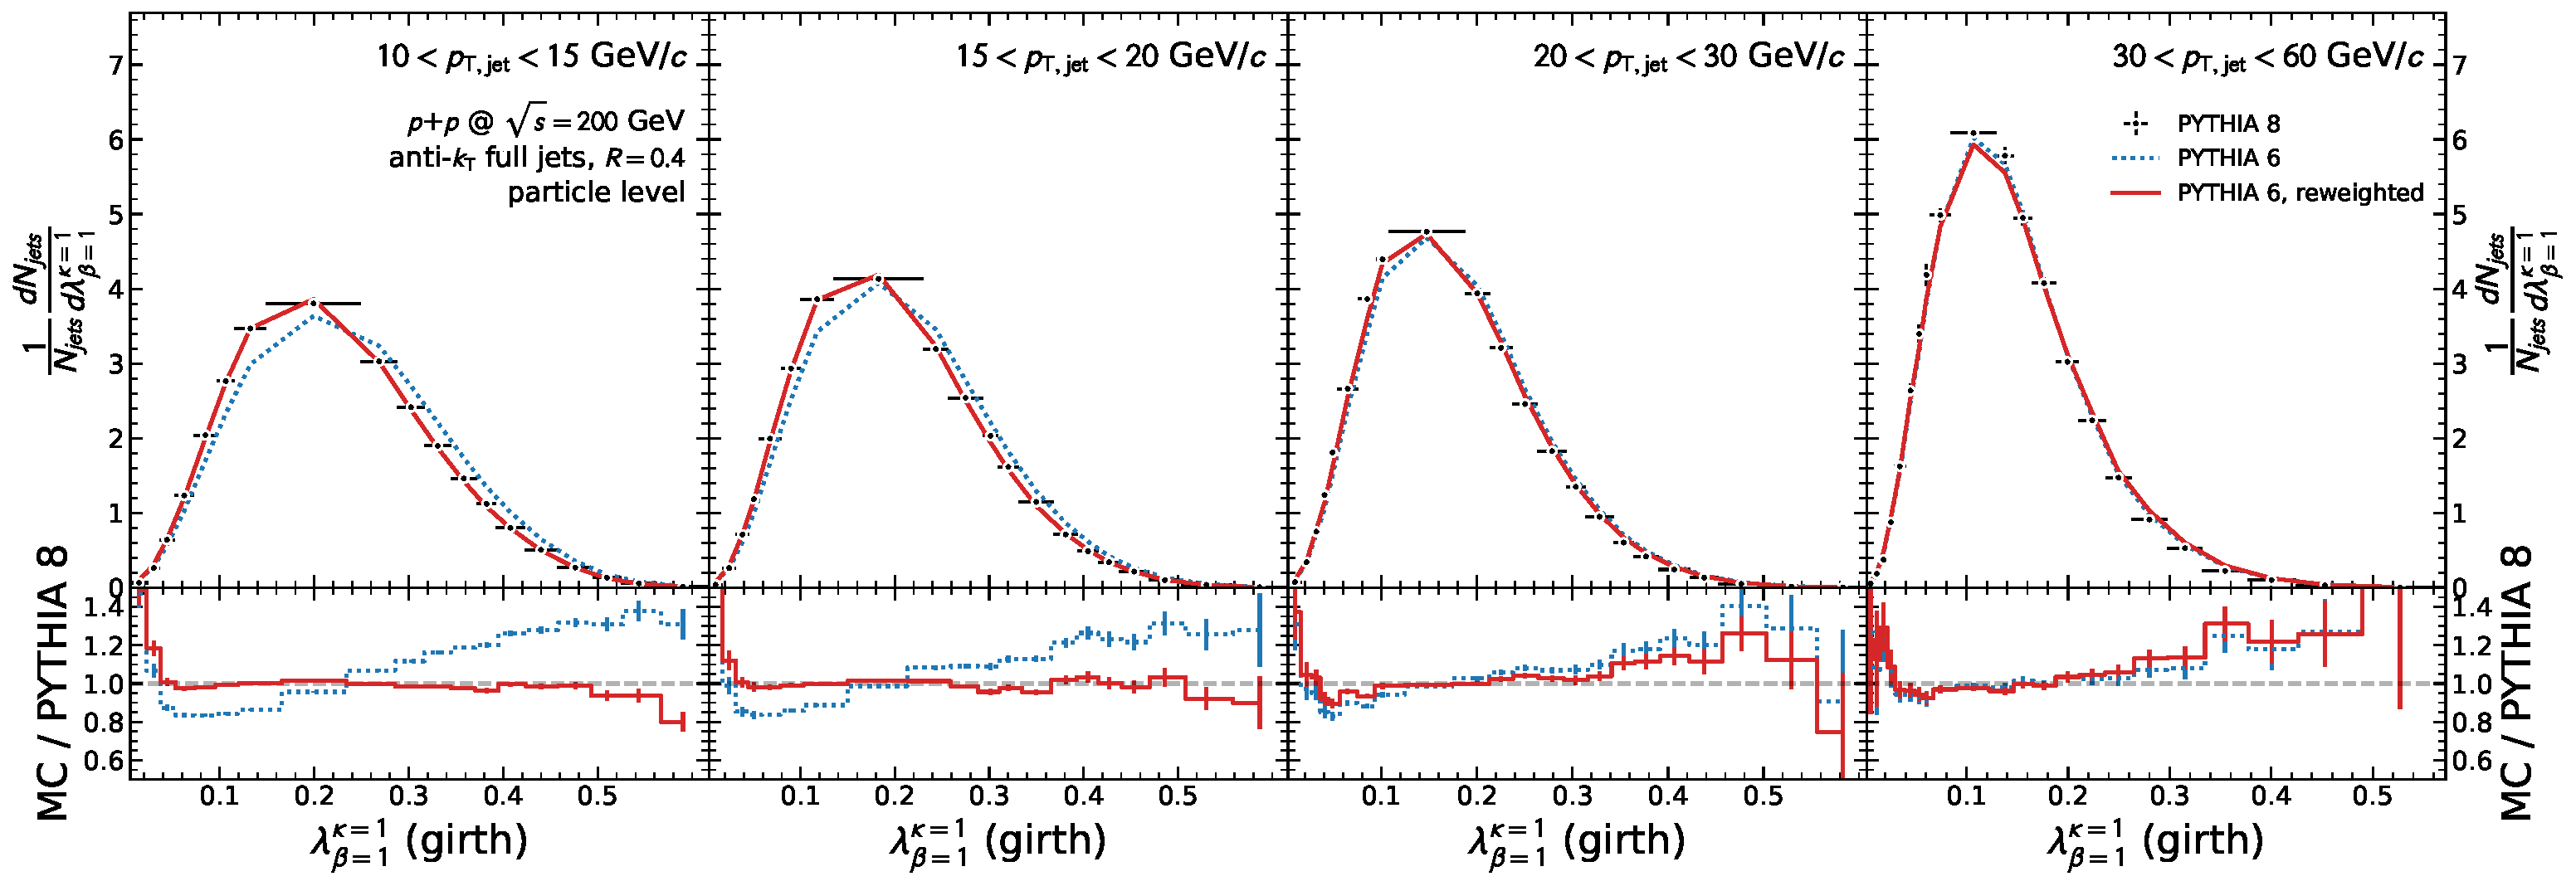
\includegraphics[width=\linewidth]{figures/angularities/pp/reweight_pythia8_ch_ang_k1_b1.pdf}&
 		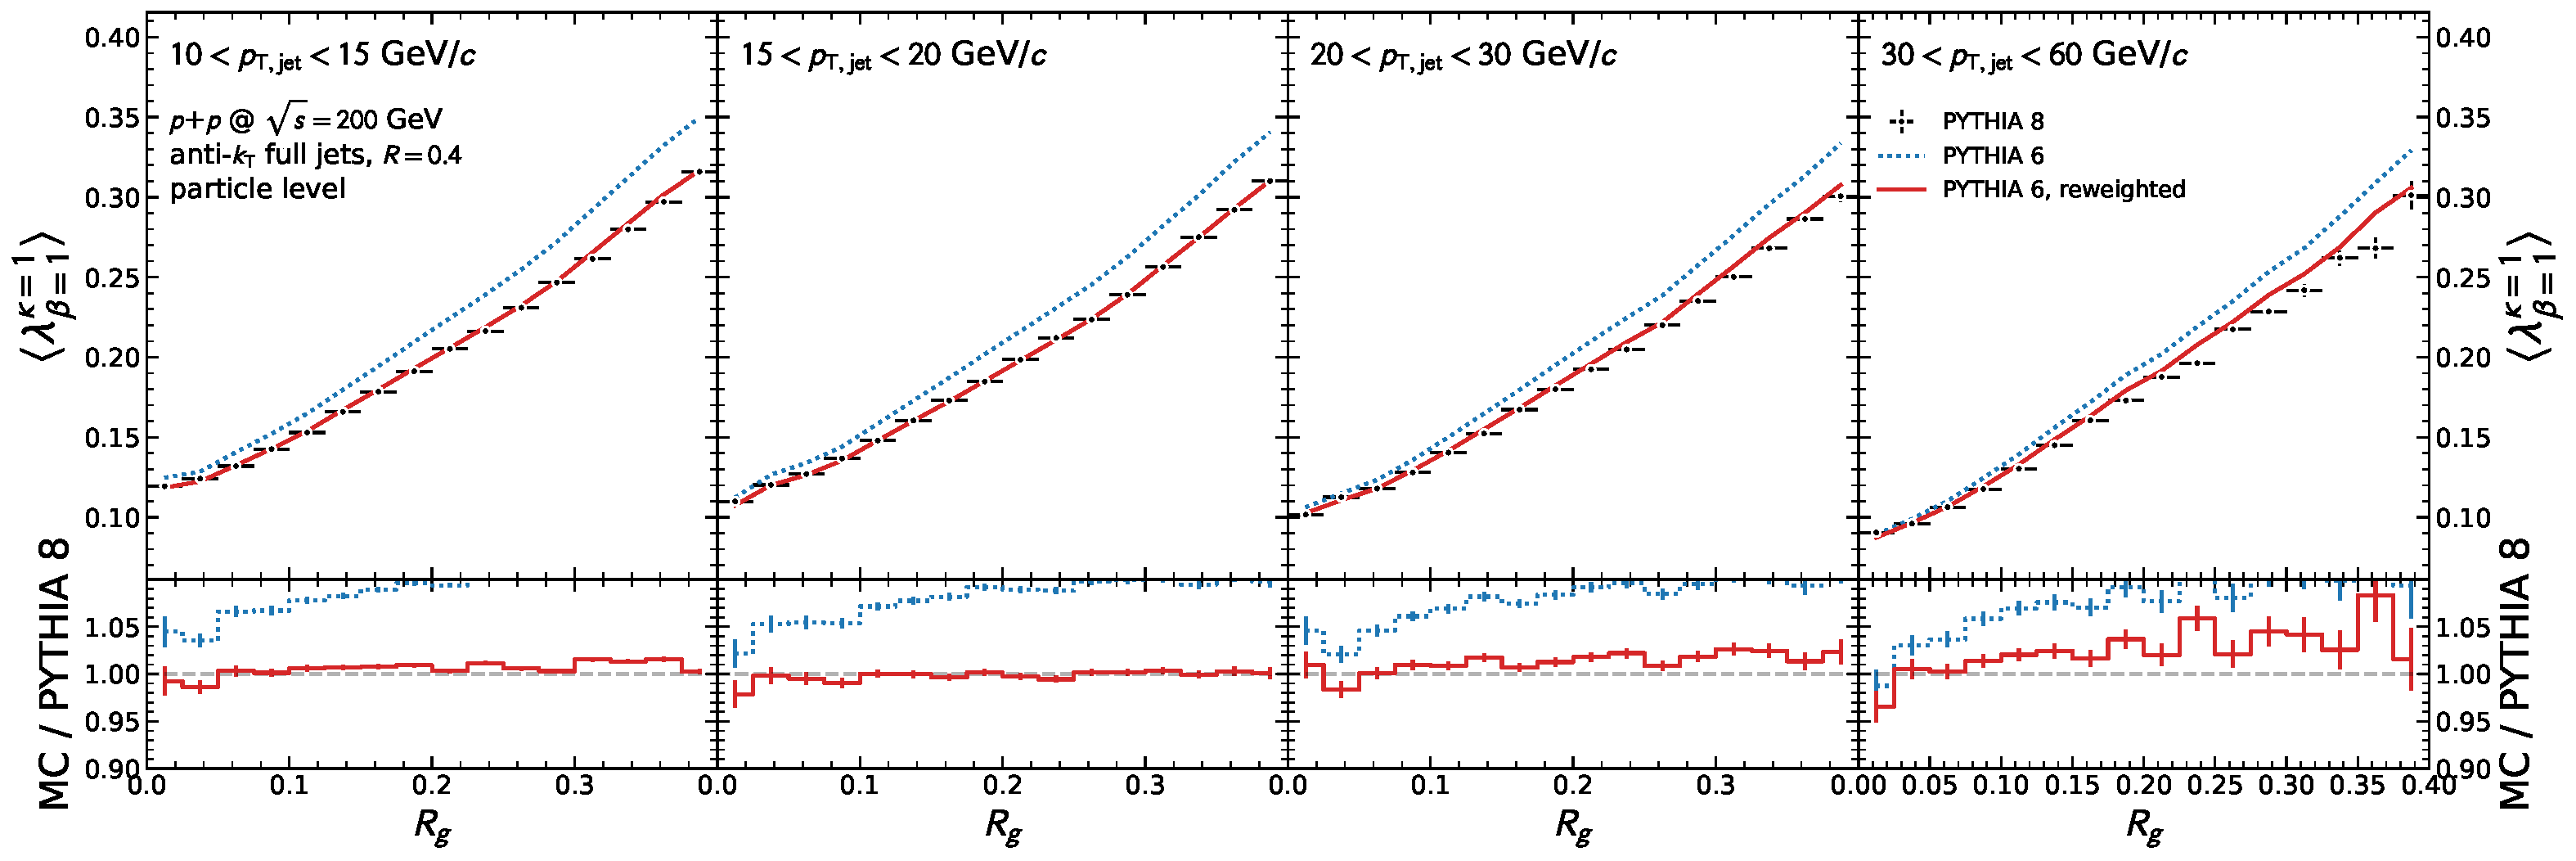
\includegraphics[width=\linewidth]{figures/angularities/pp/reweight_pythia8_prof_ch_ang_k1_b1.pdf}\\
 		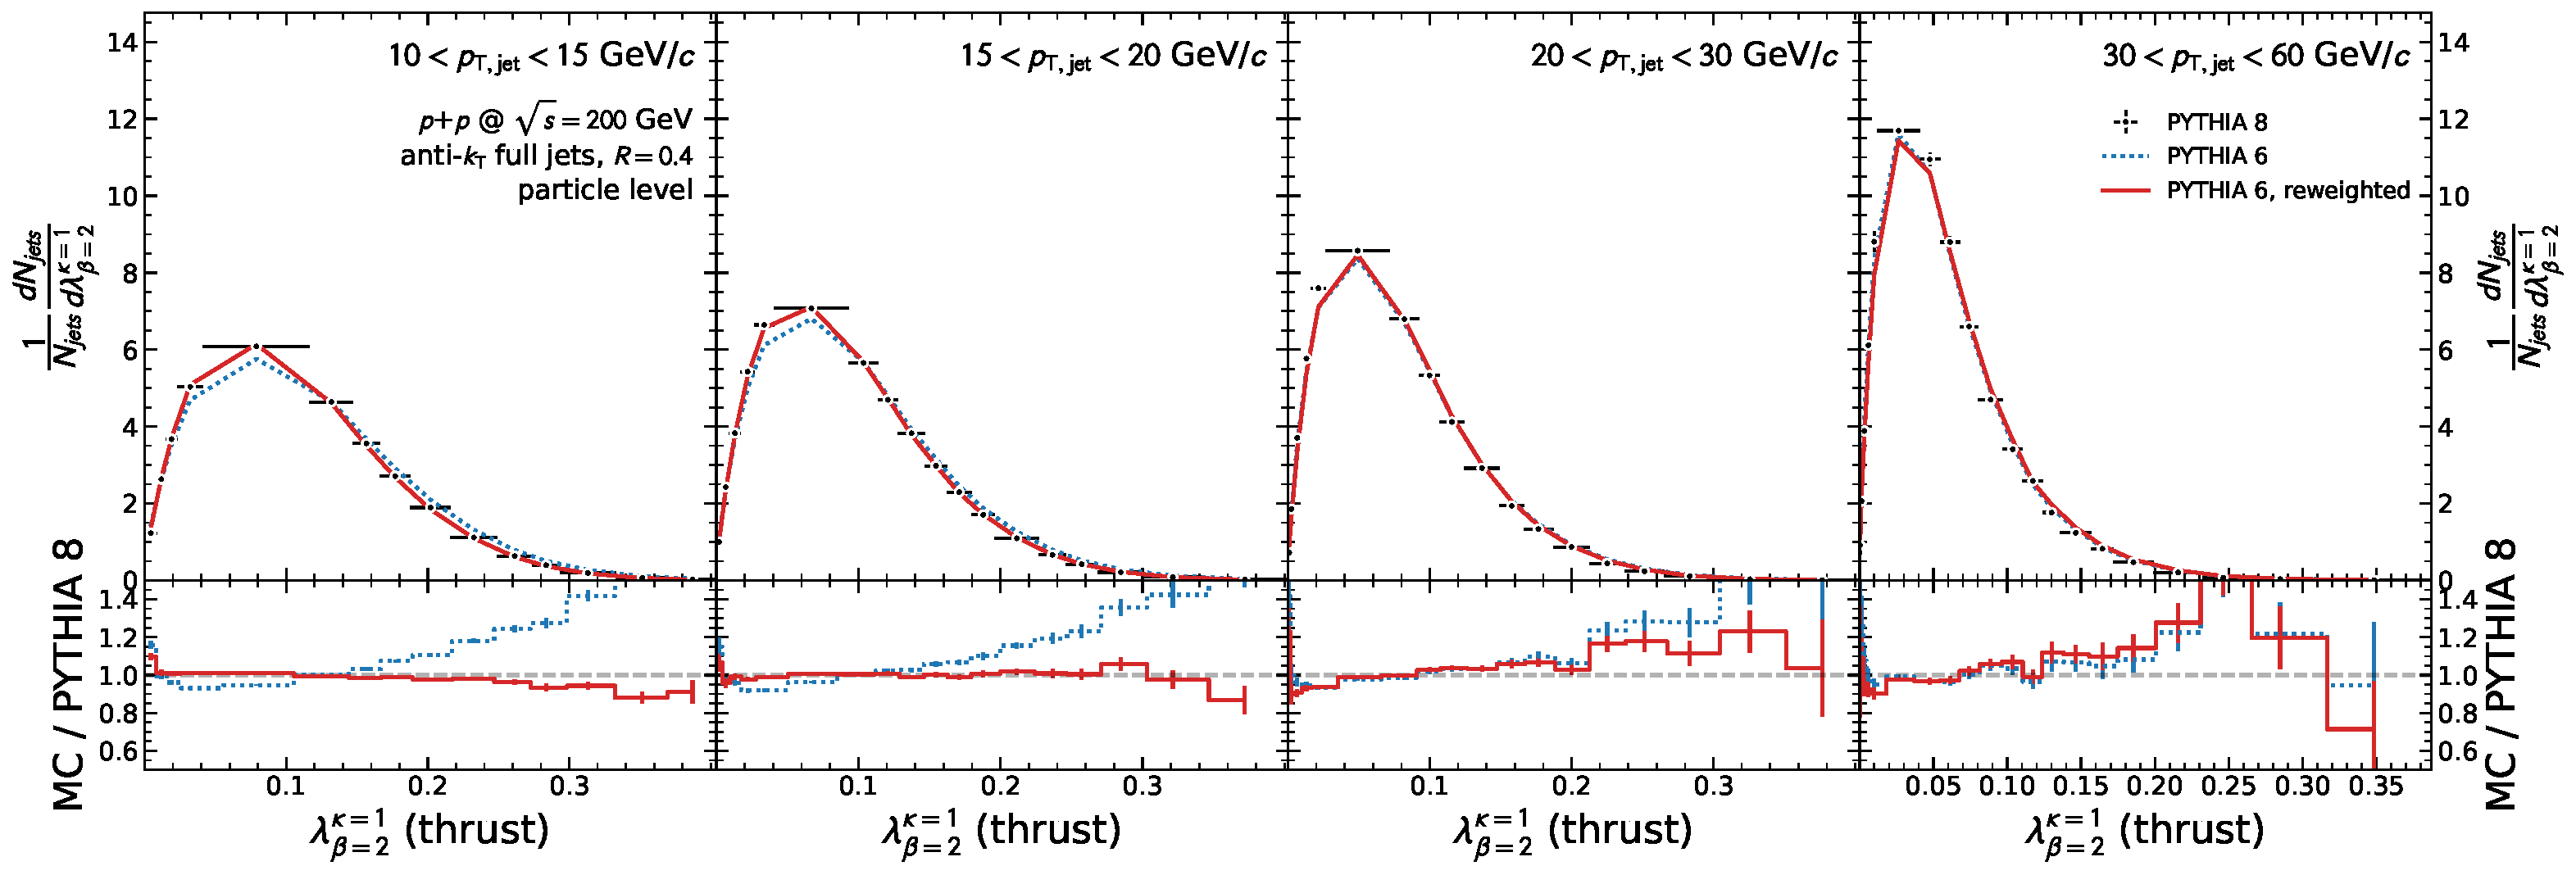
\includegraphics[width=\linewidth]{figures/angularities/pp/reweight_pythia8_ch_ang_k1_b2.pdf}&
 		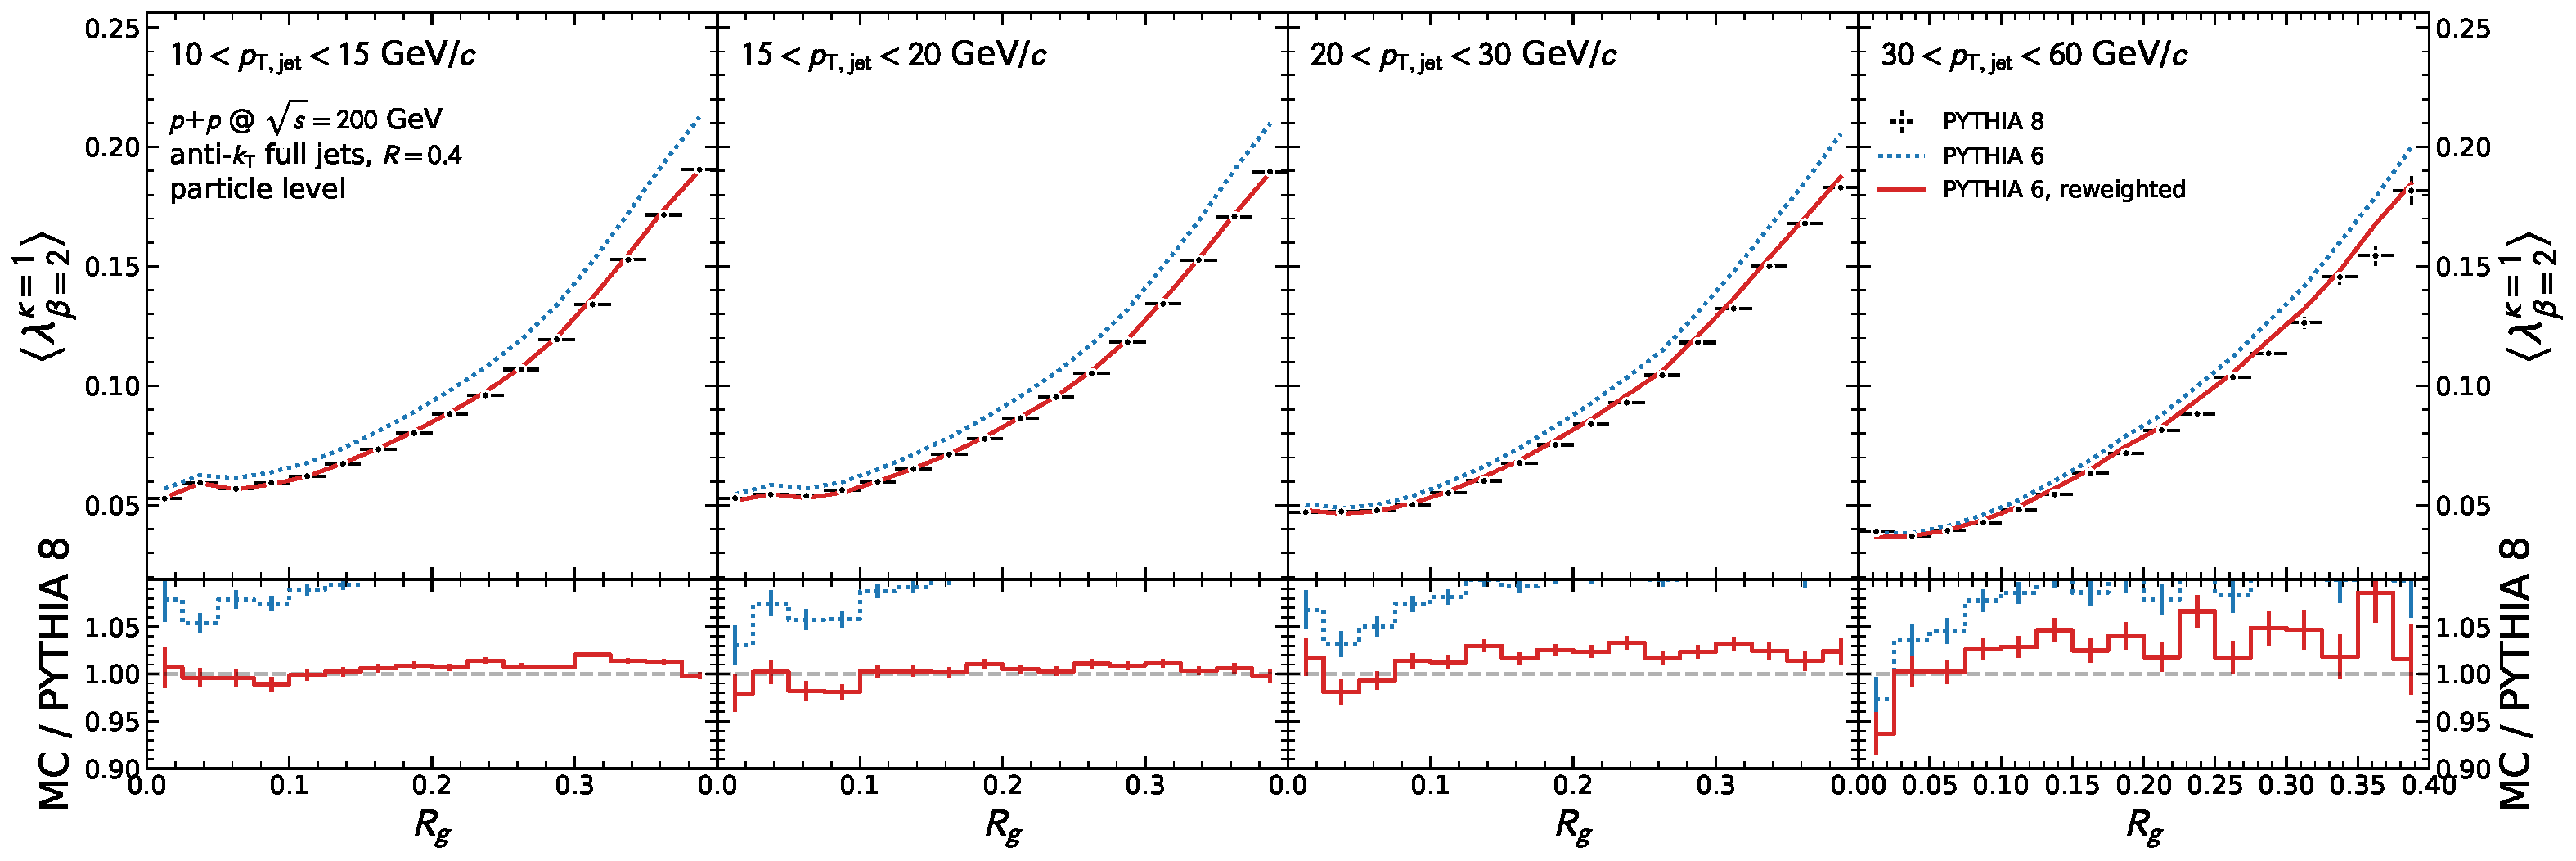
\includegraphics[width=\linewidth]{figures/angularities/pp/reweight_pythia8_prof_ch_ang_k1_b2.pdf}
 	\end{tabularx}
 	\caption{Reweighting of the PYTHIA-6 prior to PYTHIA-8 at particle level: the distributions of \(\lambda^{\kappa=1}_{\beta}\) (left) and the \(\langle\lambda^{\kappa=1}_{\beta}\rangle\) vs.\ \(R_\mathrm{g}\) profiles (right) for \(\beta = 0.5\), 1 and 2 (top to bottom), in four \(p_\mathrm{T, jet}\) ranges (panels). PYTHIA-8 (points) is compared to the nominal (dotted) and the reweighted (solid) PYTHIA-6; the lower panels show their ratios to PYTHIA-8.}
 	\label{fig:reweight_pythia8}
 \end{sidewaysfigure}

 \paragraph{Data-like prior.} The pseudo-data of the closure test is obtained from a one-iteration unfolding of the measured data by the same method.
 %
 First, a classifier separating measured from reconstructed PYTHIA6 jets (matched and fake) gives \(r(\mathbf{y}) \approx p_\mathrm{meas.}(\mathbf{y})/p_{\mathrm{reco.}, 0}(\mathbf{y})\), which is applied to the reconstructed jets.
 %
 Matched generated jets inherit the weight of their reconstructed partner.
 %
 As missed jets have none, a second classifier separates the matched generated jets weighted this way from the unweighted ones, and the resulting smooth \(r(\mathbf{x})\) is applied to all generated jets, matched and missed.
 %
 The reweighted reconstructed jets are the pseudo-data, the reweighted generated jets the pseudo-truth, and the pseudo-data are unfolded with the nominal PYTHIA6 embedding.
 %
 Since the pseudo-data resemble the measurement, but the pseudo-truth is known, the deviation of the pseudo-unfolded result from the pseudo-truth (Figs.~\ref{fig:ClosureAngularity} and \ref{fig:ClosureAngVsRg}) is a non-closure uncertainty applied to the measured result as a relative uncertainty.
 
 \begin{figure}
 	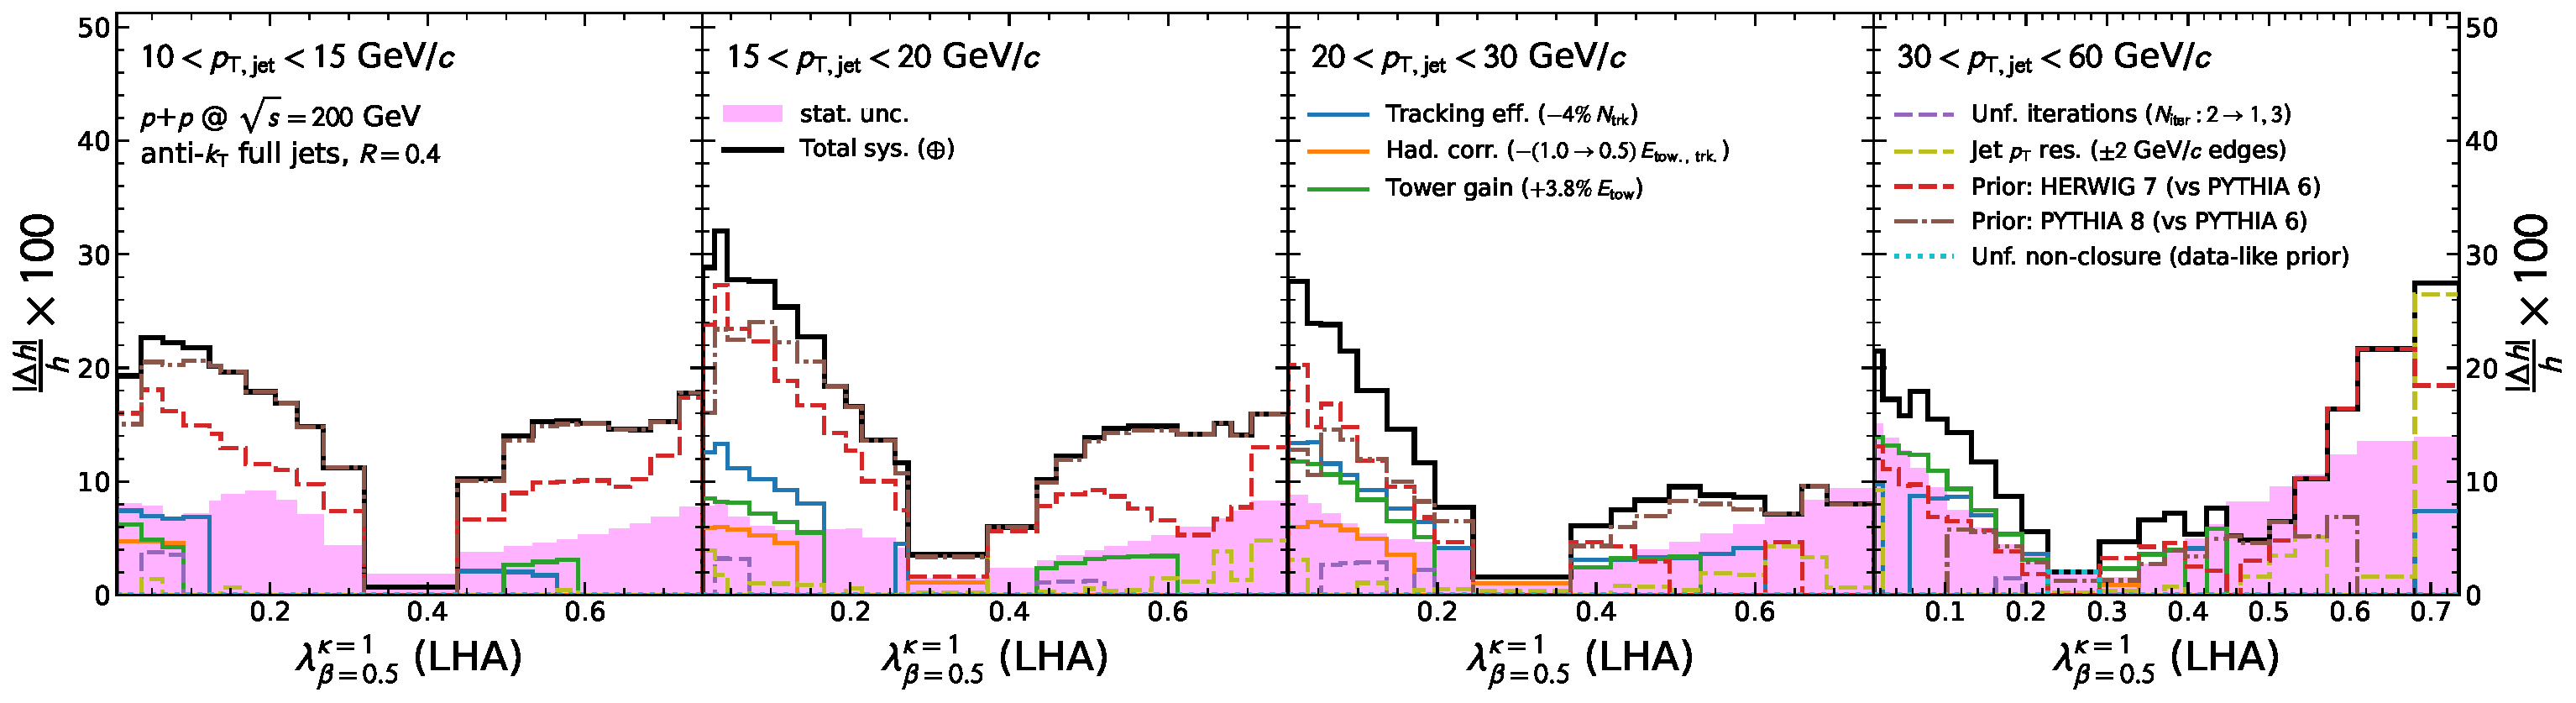
\includegraphics[width=\textwidth]{angularities/pp/sys_ch_ang_k1_b0.5_hist_ang.pdf}
 	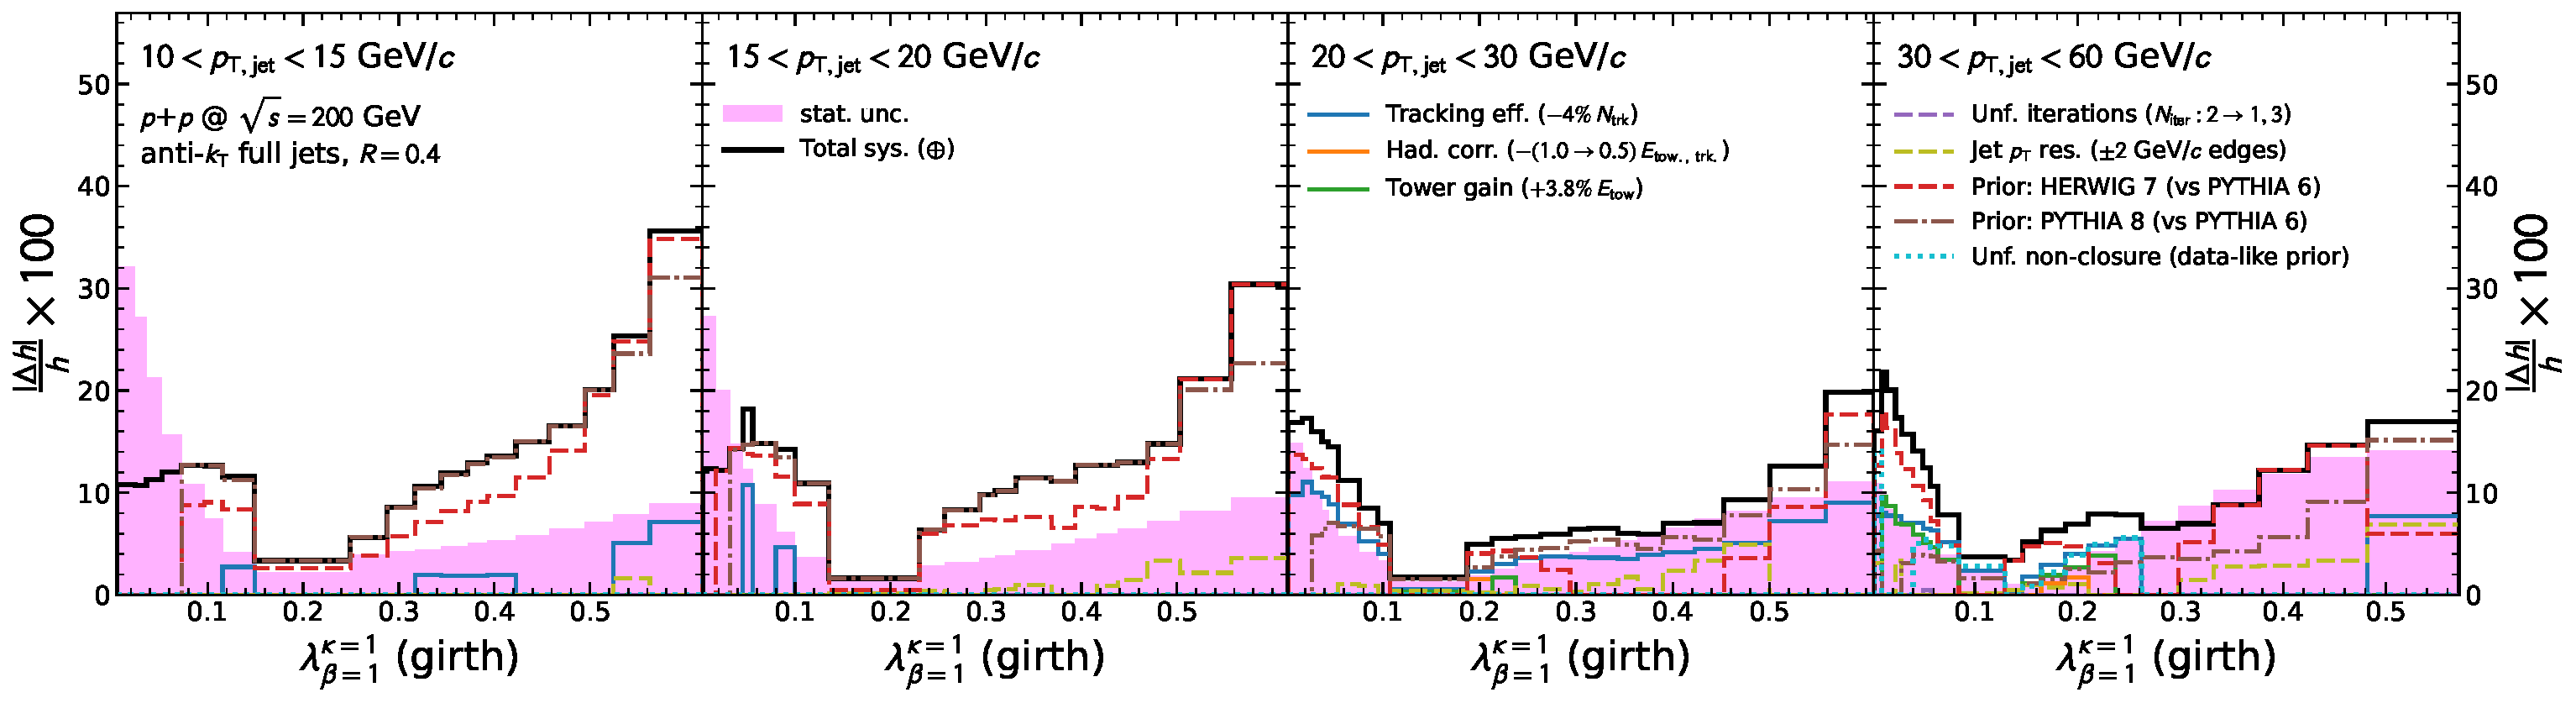
\includegraphics[width=\textwidth]{angularities/pp/sys_ch_ang_k1_b1_hist_ang.pdf}
 	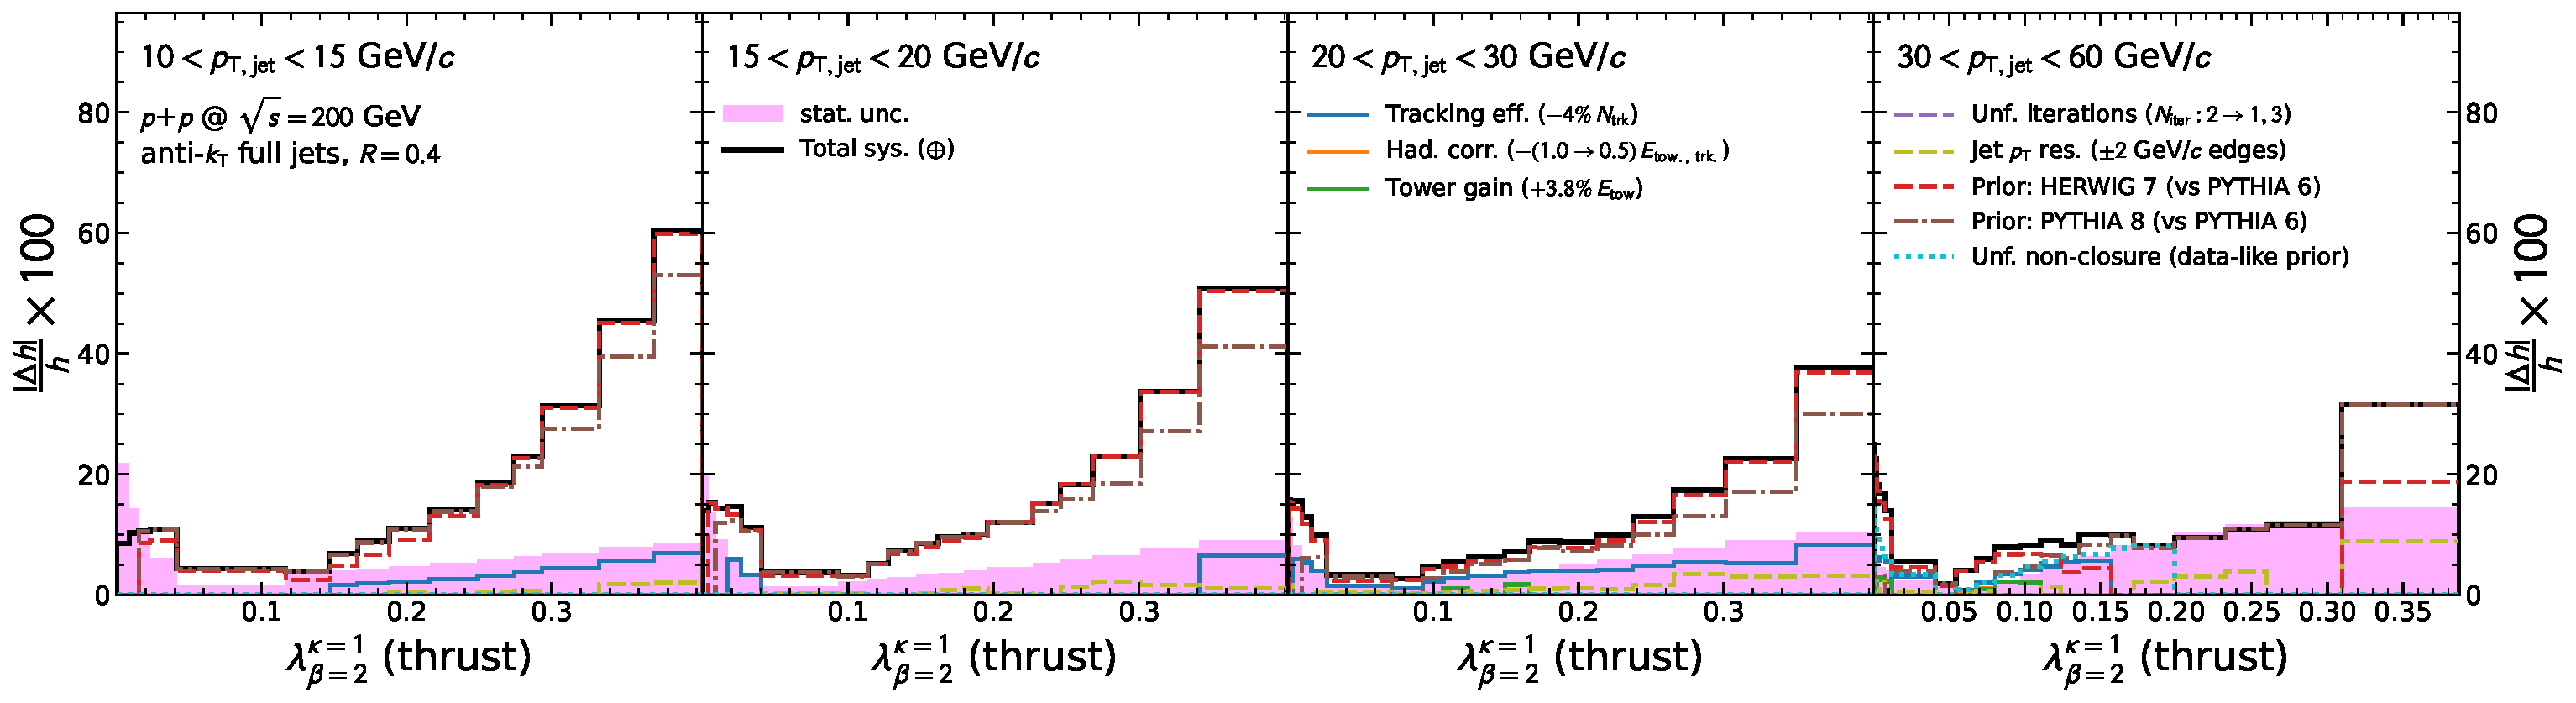
\includegraphics[width=\linewidth]{angularities/pp/sys_ch_ang_k1_b2_hist_ang.pdf}
	\caption{Relative systematic uncertainties of the \(\lambda^{\kappa=1}_{\beta}\) distributions of inclusive jets, after the Barlow check (Sec.~\ref{sec:barlow}), for \(\beta = 0.5\), 1 and 2 (top to bottom). The sources are the tracking efficiency, the hadronic correction and the tower gain (solid), the number of unfolding iterations, the jet-\(p_\mathrm{T}\) resolution and the HERWIG-7 and PYTHIA-8 priors (dashed), and the non-closure (dotted); the black line is their sum in quadrature and the magenta band is the statistical uncertainty. Jet-\(p_\mathrm{T}\) ranges are shown as panels.}
	\label{fig:SysDistIncl}
\end{figure}
 \begin{figure}
 	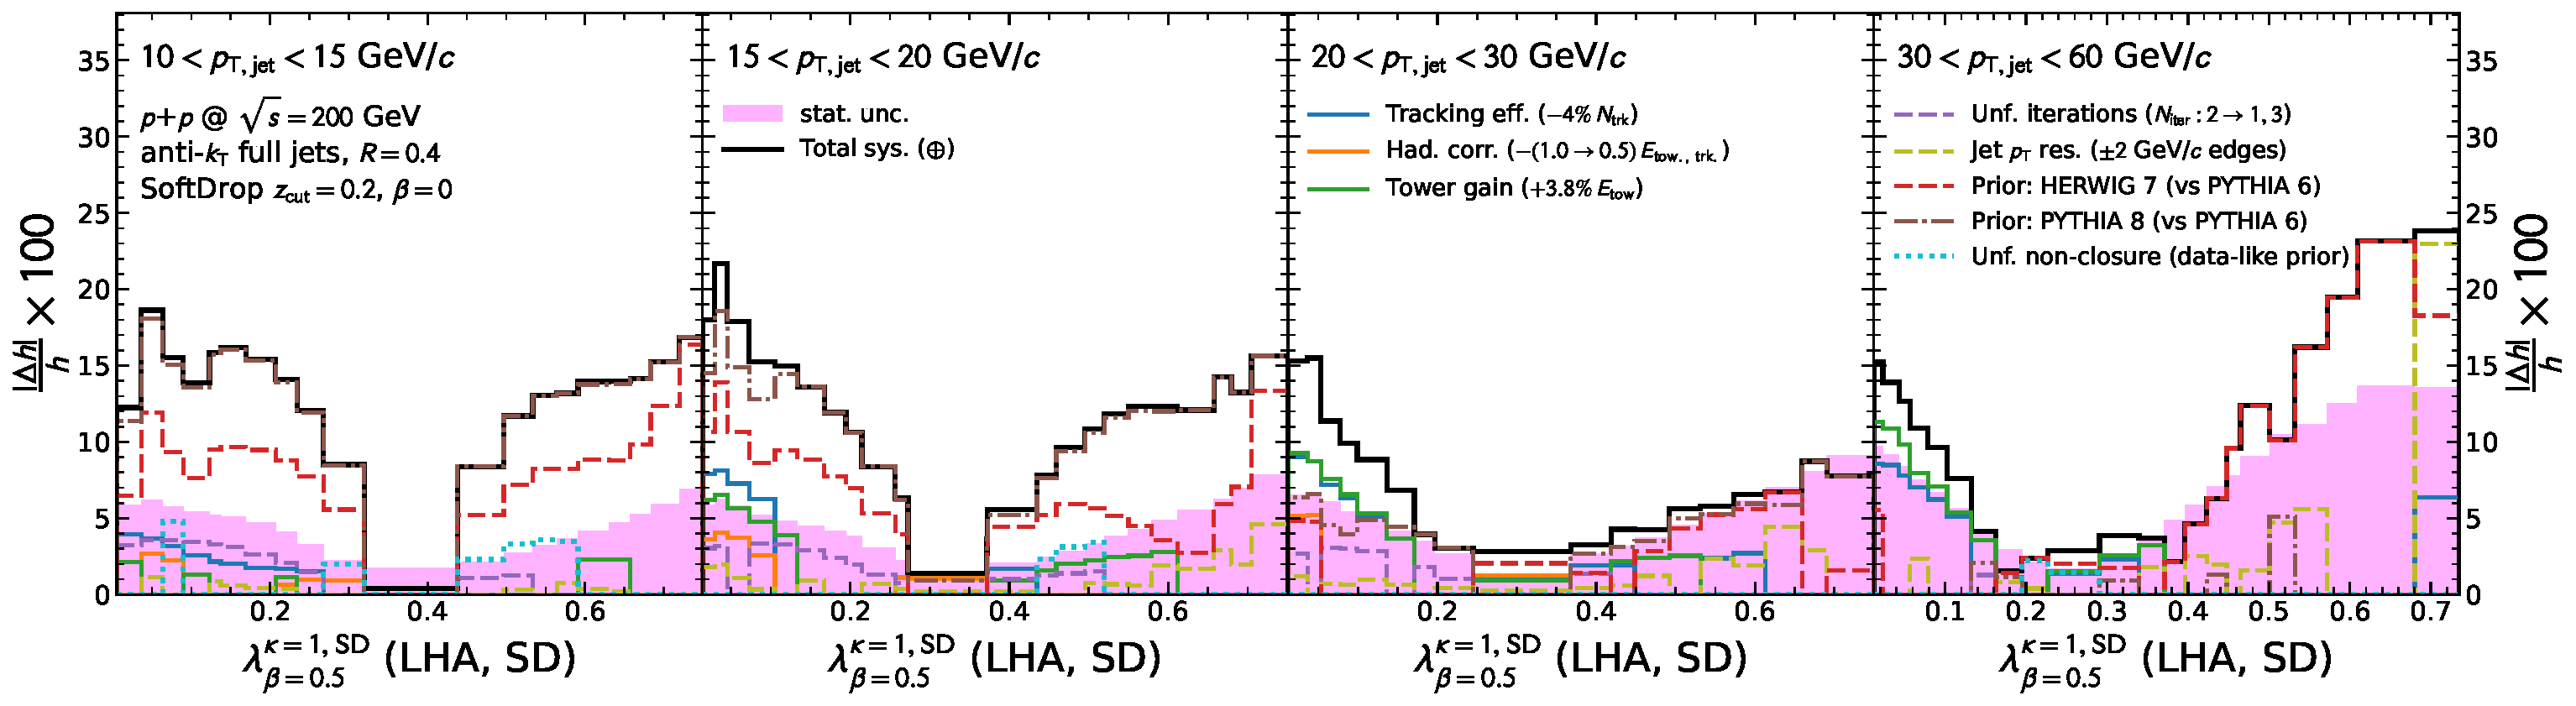
\includegraphics[width=\linewidth]{angularities/pp/sys_ch_ang_k1_b0.5_hist_sd_ang.pdf}
 	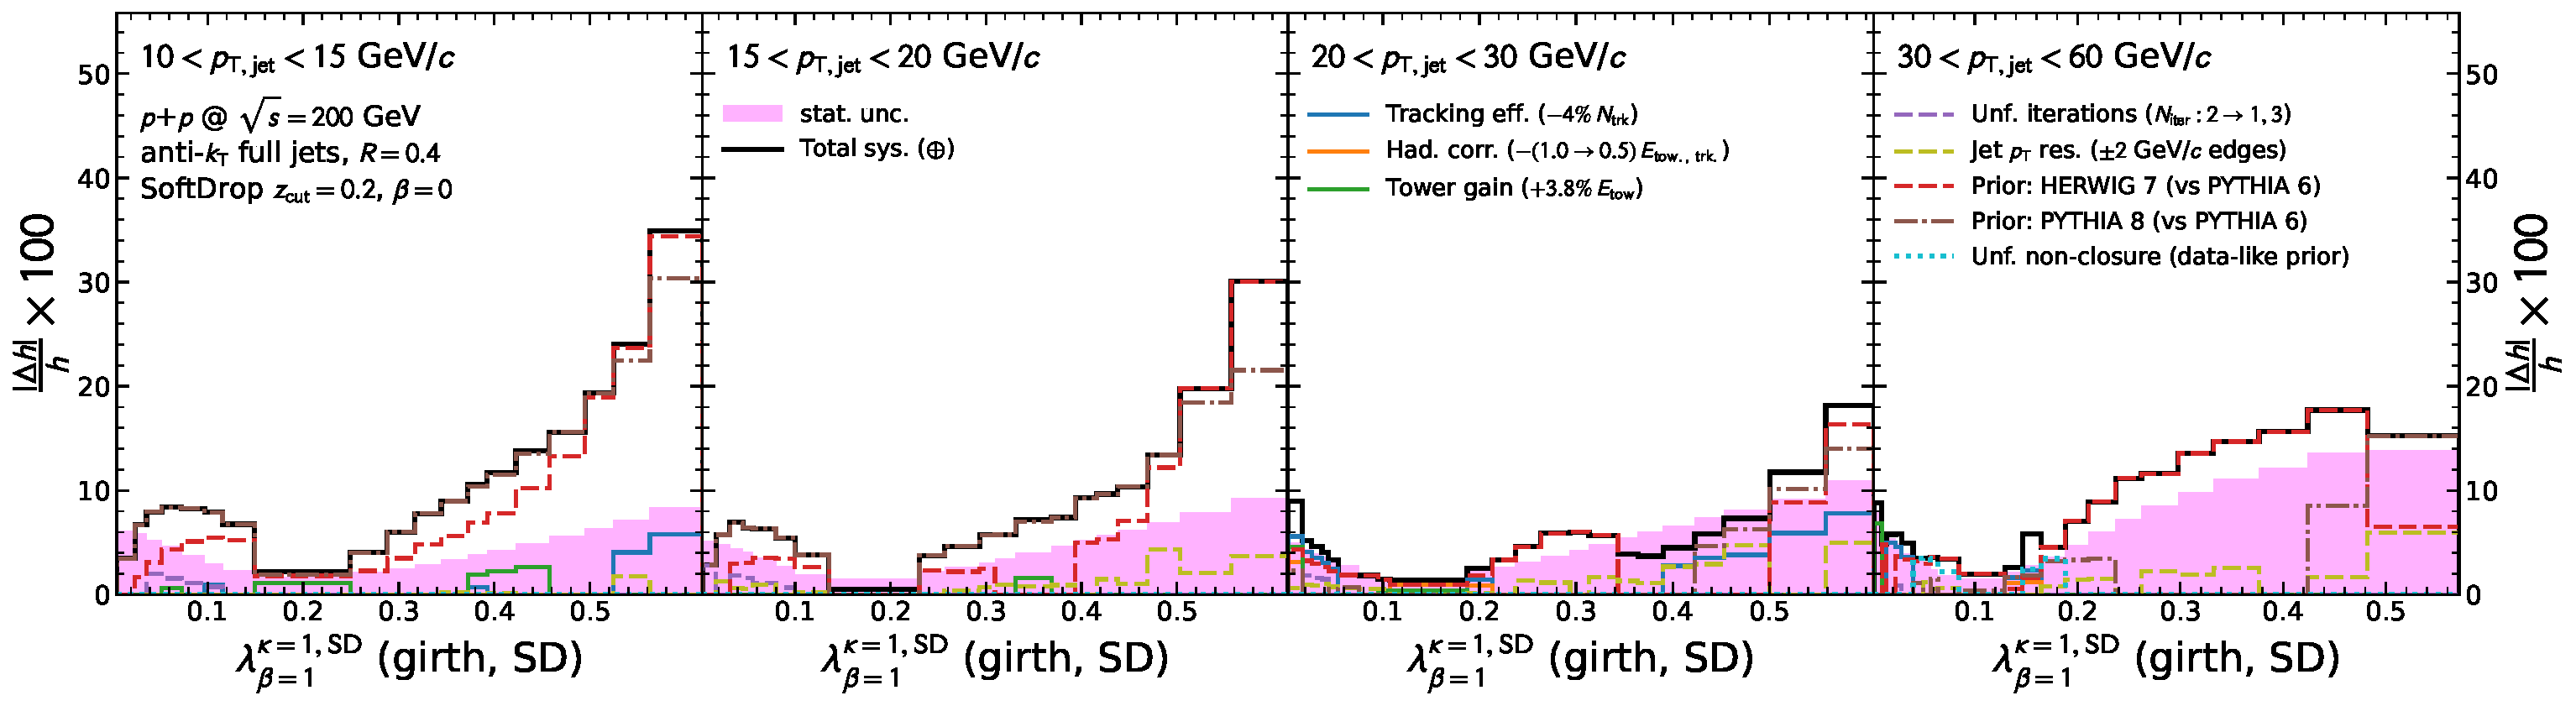
\includegraphics[width=\linewidth]{angularities/pp/sys_ch_ang_k1_b1_hist_sd_ang.pdf}
 	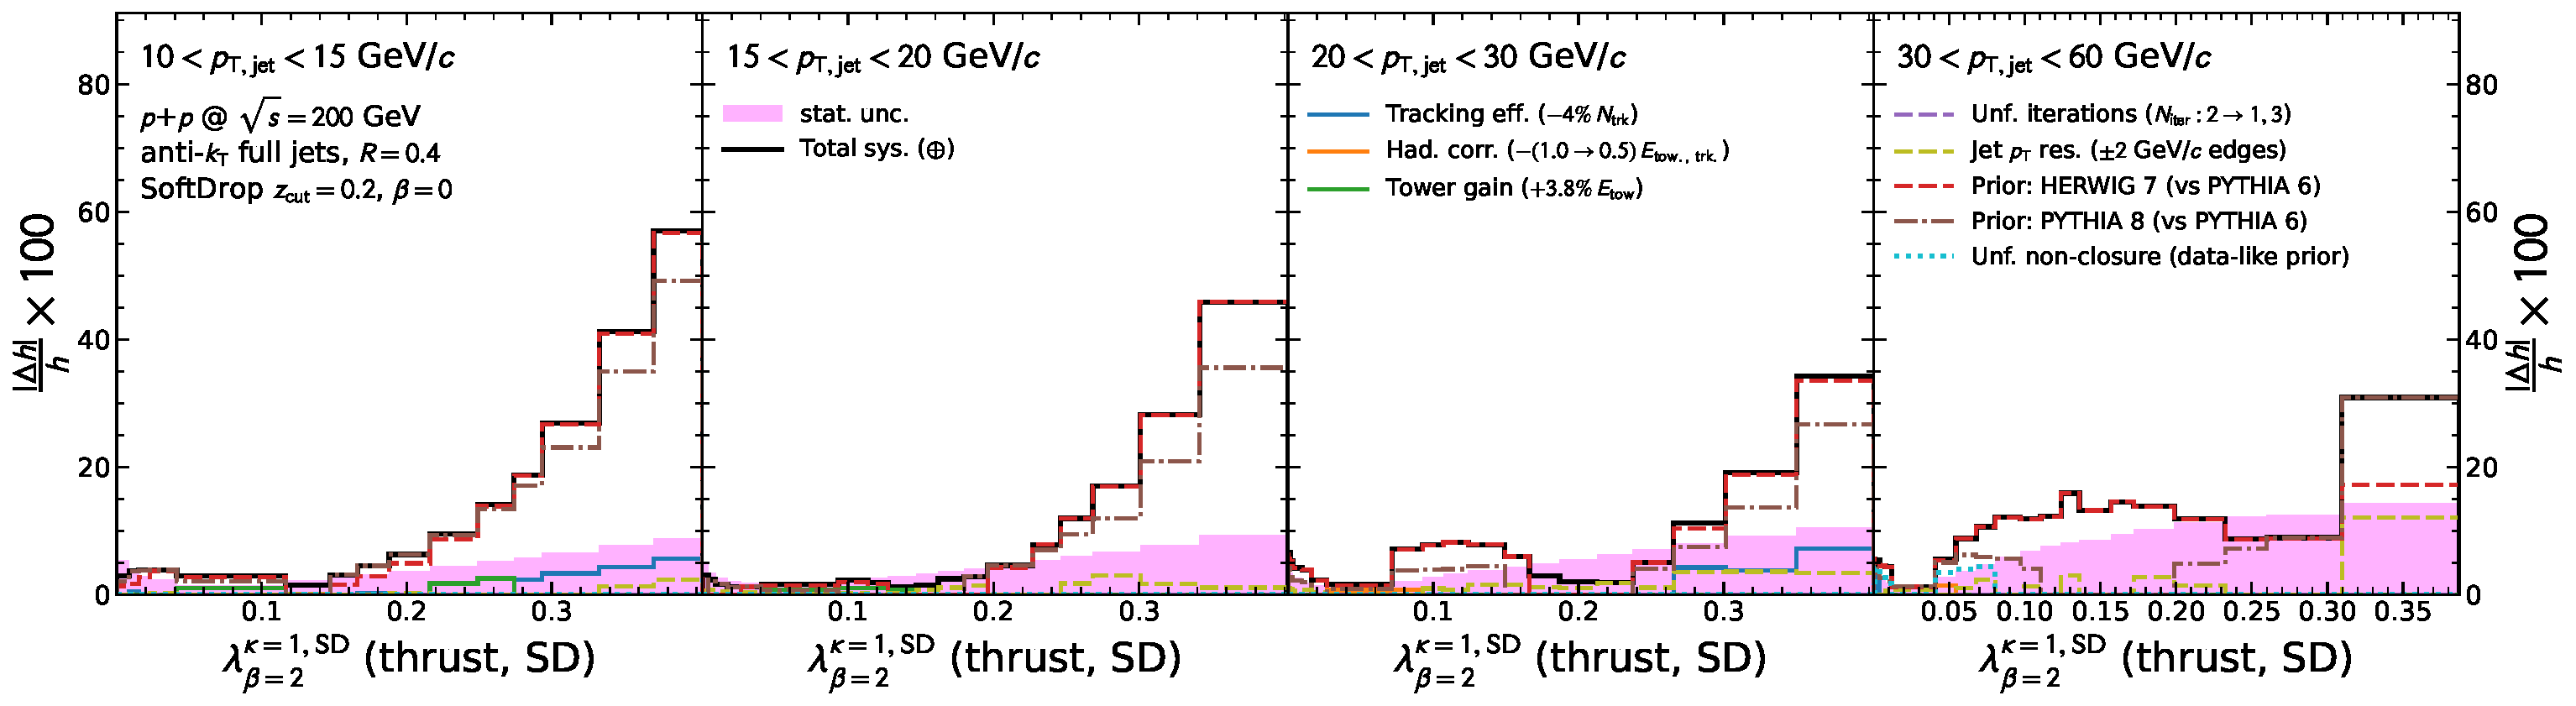
\includegraphics[width=\linewidth]{angularities/pp/sys_ch_ang_k1_b2_hist_sd_ang.pdf}
	\caption{Relative systematic uncertainties of the \(\lambda^{\kappa=1}_{\beta}\) distributions of SoftDrop-groomed jets, after the Barlow check (Sec.~\ref{sec:barlow}), for \(\beta = 0.5\), 1 and 2 (top to bottom). The sources are the tracking efficiency, the hadronic correction and the tower gain (solid), the number of unfolding iterations, the jet-\(p_\mathrm{T}\) resolution and the HERWIG-7 and PYTHIA-8 priors (dashed), and the non-closure (dotted); the black line is their sum in quadrature and the magenta band is the statistical uncertainty. Jet-\(p_\mathrm{T}\) ranges are shown as panels.}
	\label{fig:SysDistSD}
\end{figure}
 \begin{figure}
 	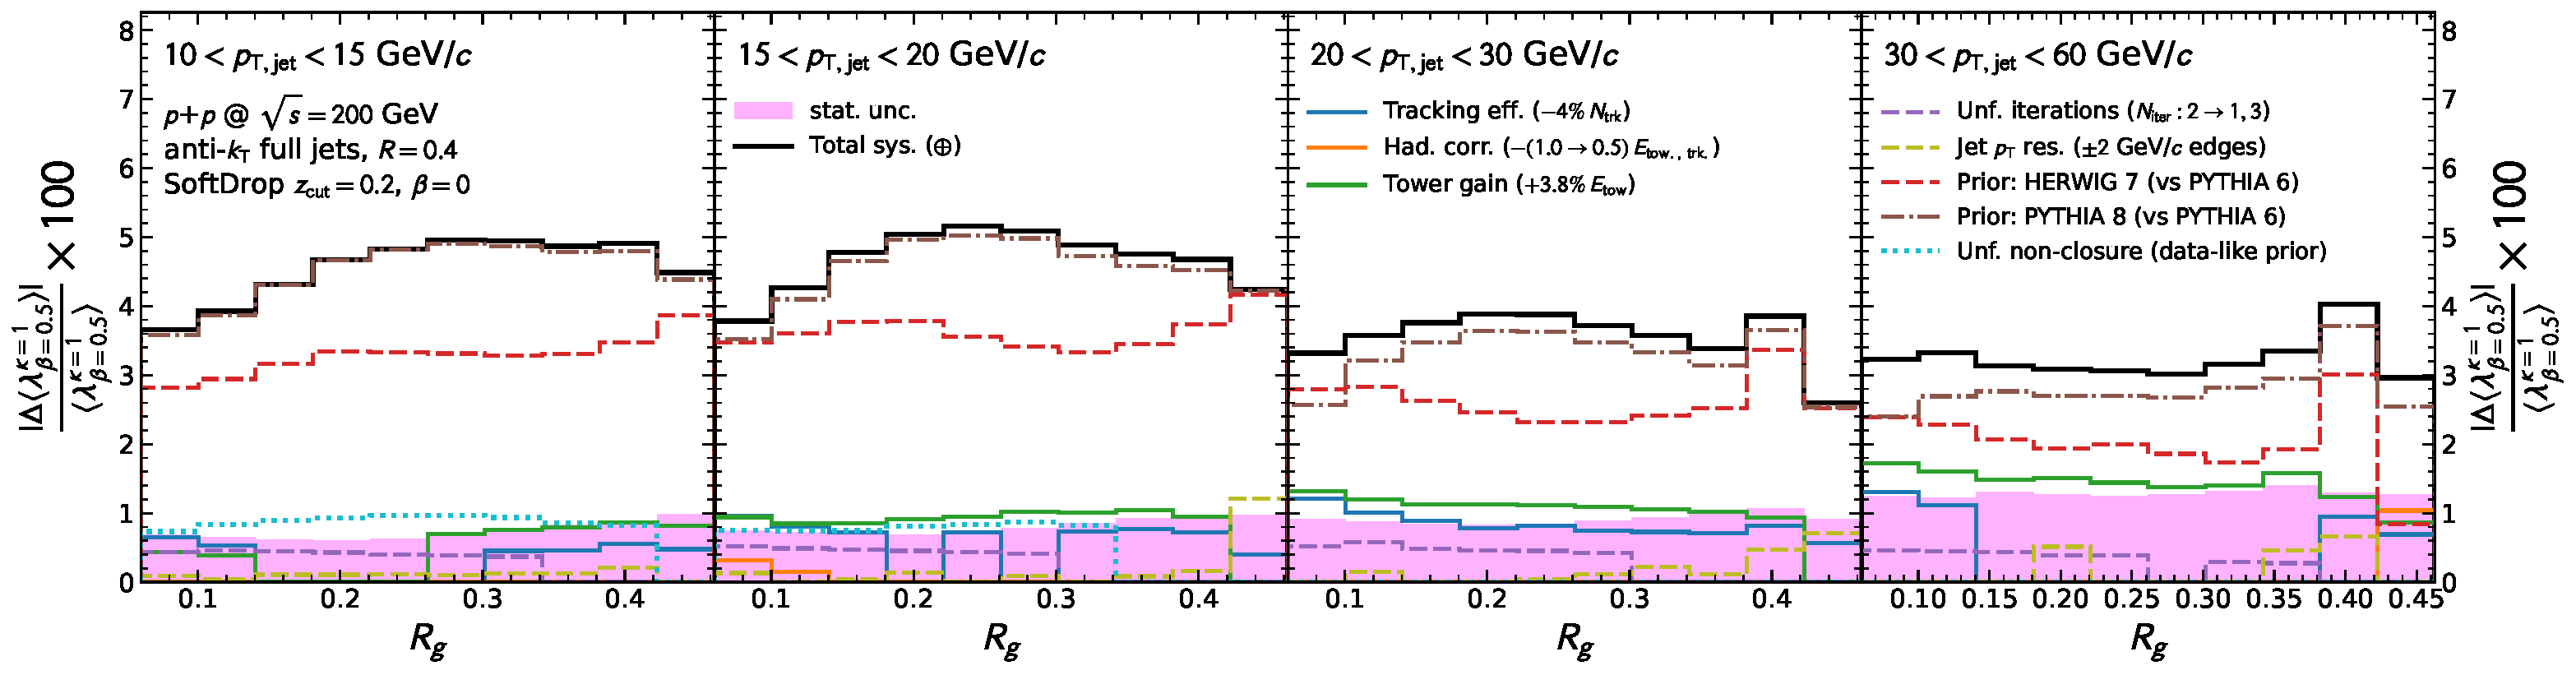
\includegraphics[width=\linewidth]{angularities/pp/sys_ch_ang_k1_b0.5_prof_incl_vs_sd_dR.pdf}
 	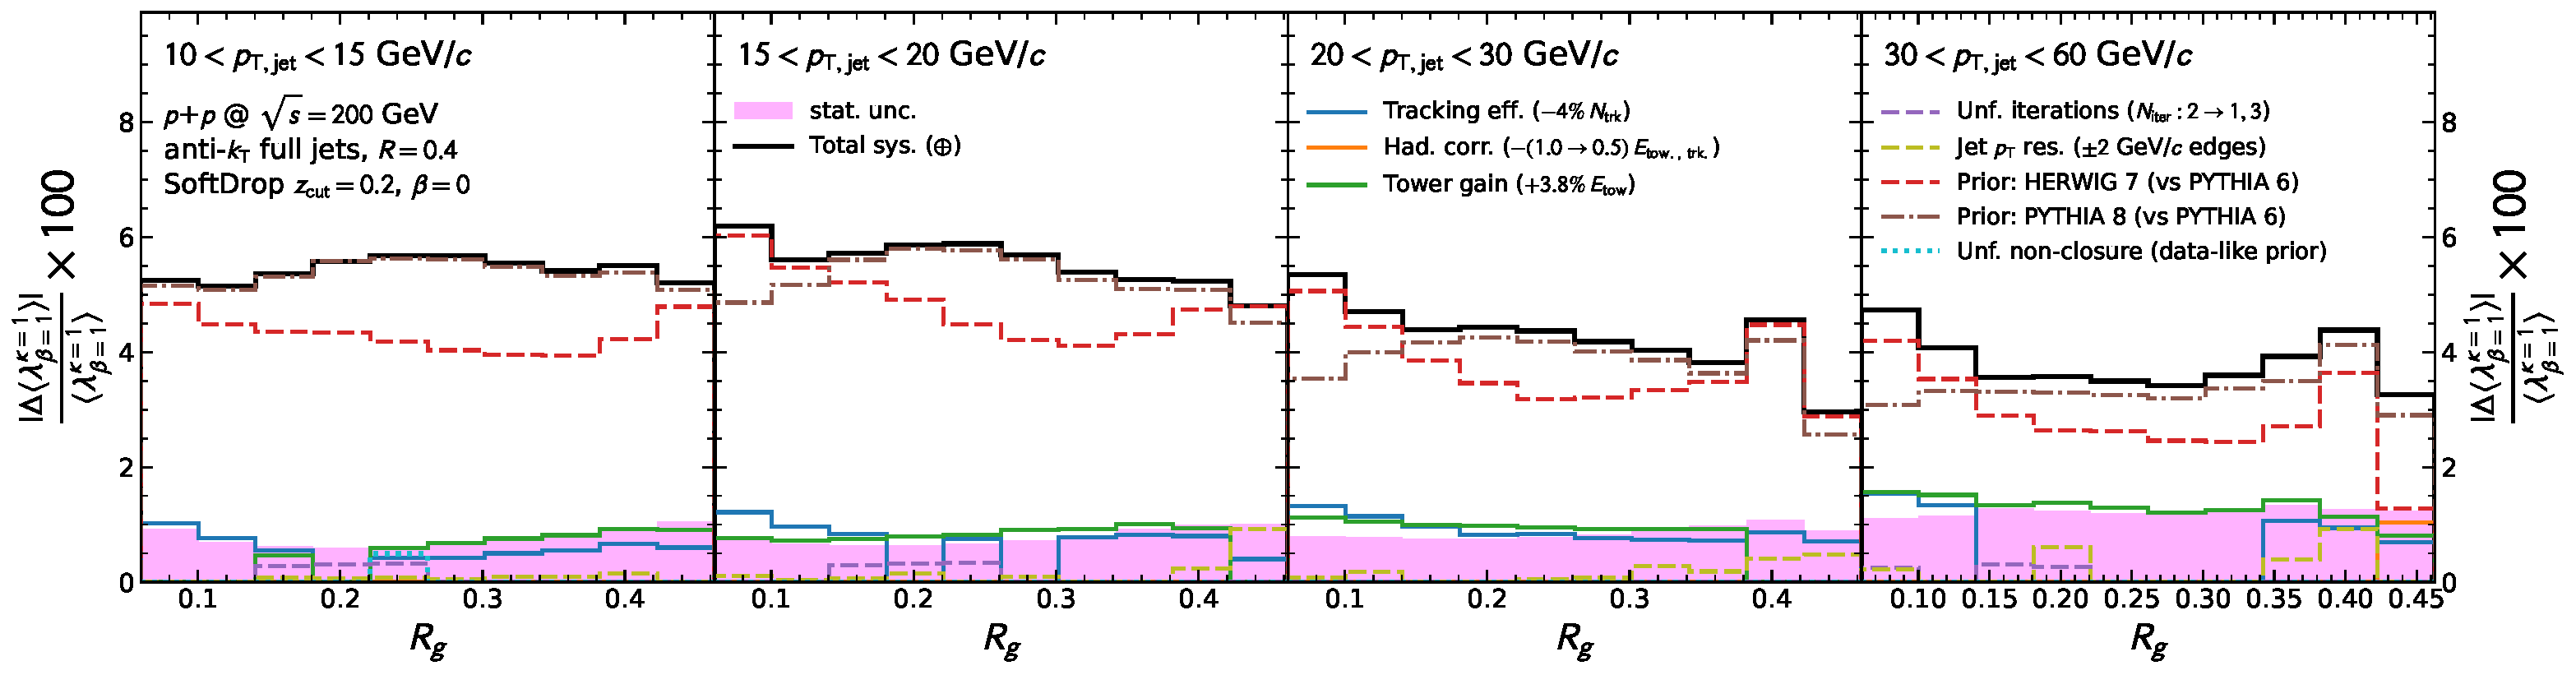
\includegraphics[width=\linewidth]{angularities/pp/sys_ch_ang_k1_b1_prof_incl_vs_sd_dR.pdf}
 	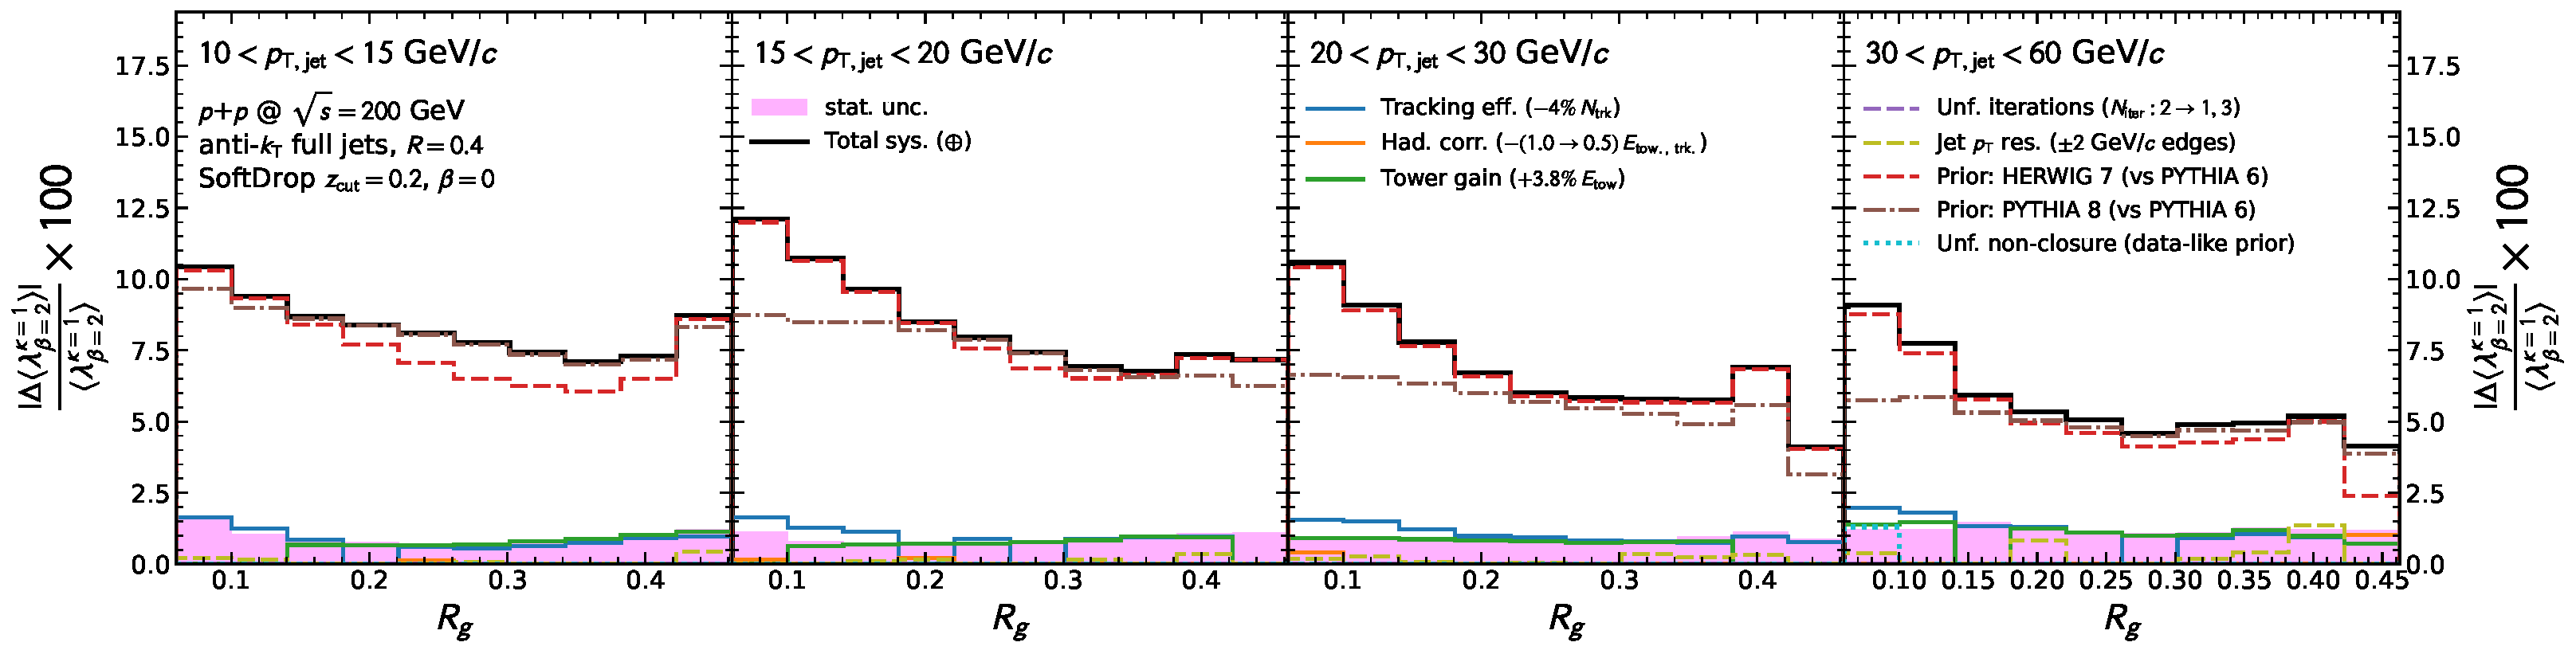
\includegraphics[width=\linewidth]{angularities/pp/sys_ch_ang_k1_b2_prof_incl_vs_sd_dR.pdf}
	\caption{Relative systematic uncertainties of the \(\langle\lambda^{\kappa=1}_{\beta}\rangle\) vs.\ \(R_\mathrm{g}\) profiles of inclusive jets, after the Barlow check (Sec.~\ref{sec:barlow}), for \(\beta = 0.5\), 1 and 2 (top to bottom). The sources are the tracking efficiency, the hadronic correction and the tower gain (solid), the number of unfolding iterations, the jet-\(p_\mathrm{T}\) resolution and the HERWIG-7 and PYTHIA-8 priors (dashed), and the non-closure (dotted); the black line is their sum in quadrature and the magenta band is the statistical uncertainty. Jet-\(p_\mathrm{T}\) ranges are shown as panels.}
	\label{fig:SysProfIncl}
\end{figure}
 \begin{figure}
 	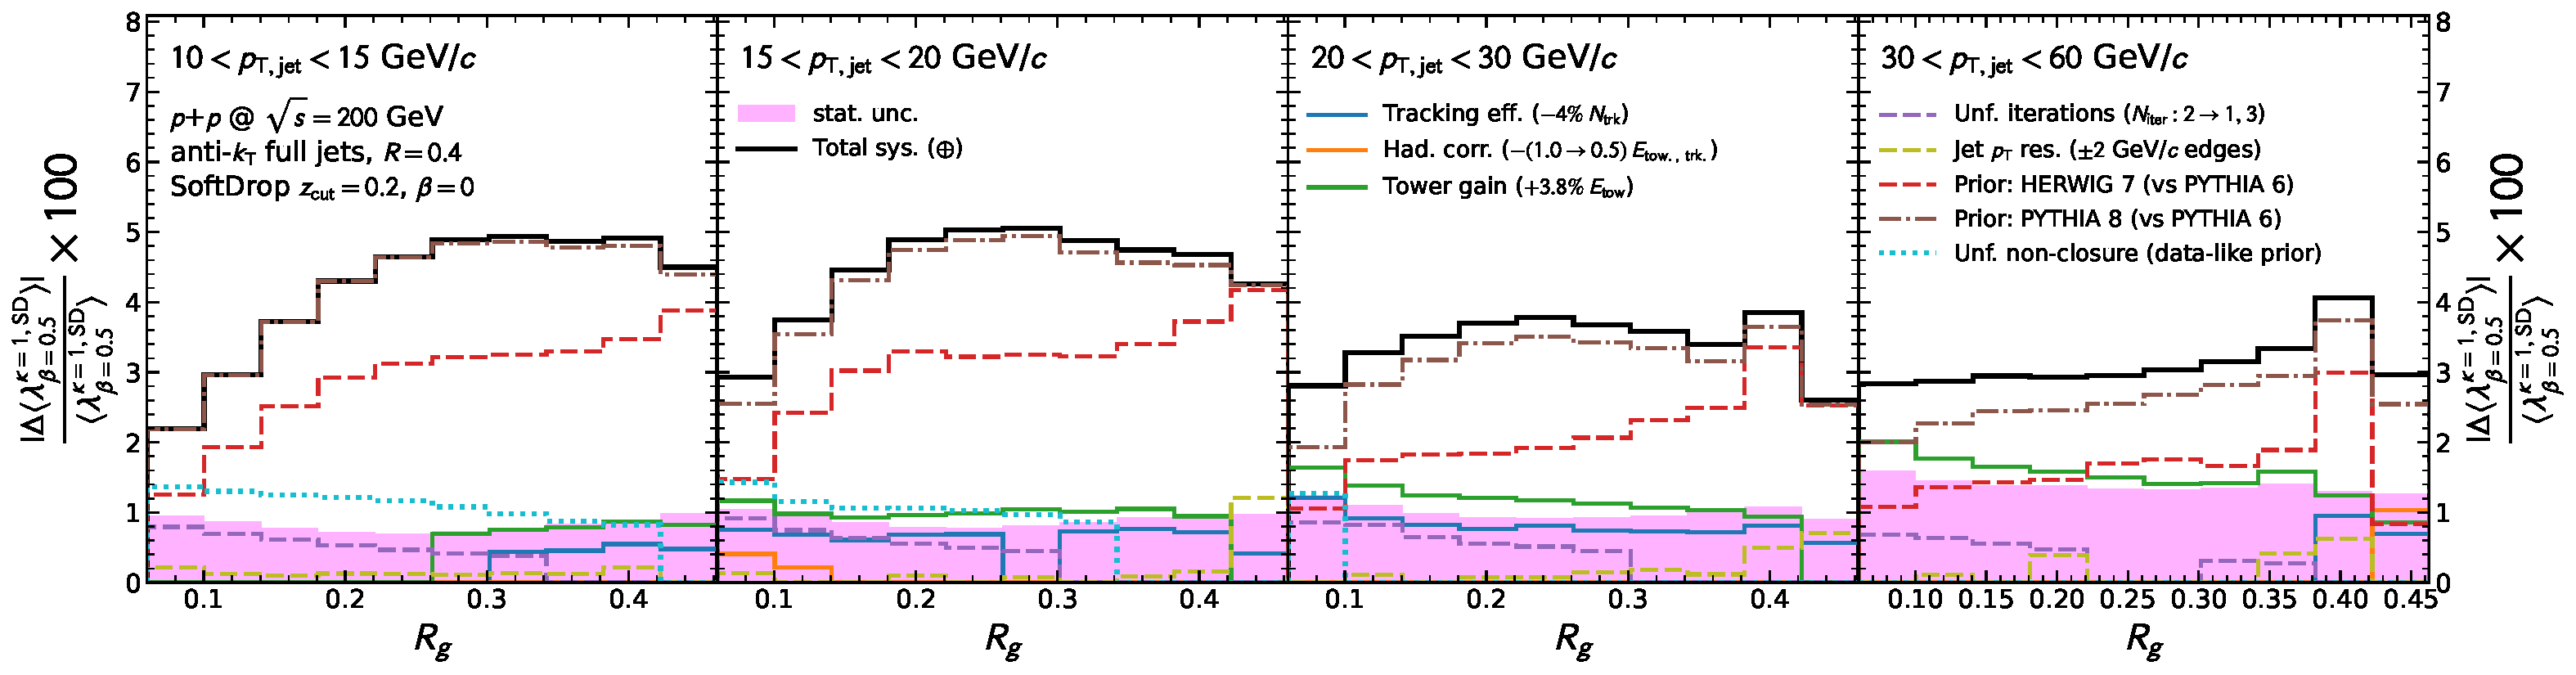
\includegraphics[width=\linewidth]{angularities/pp/sys_ch_ang_k1_b0.5_prof_sd_vs_sd_dR.pdf}
 	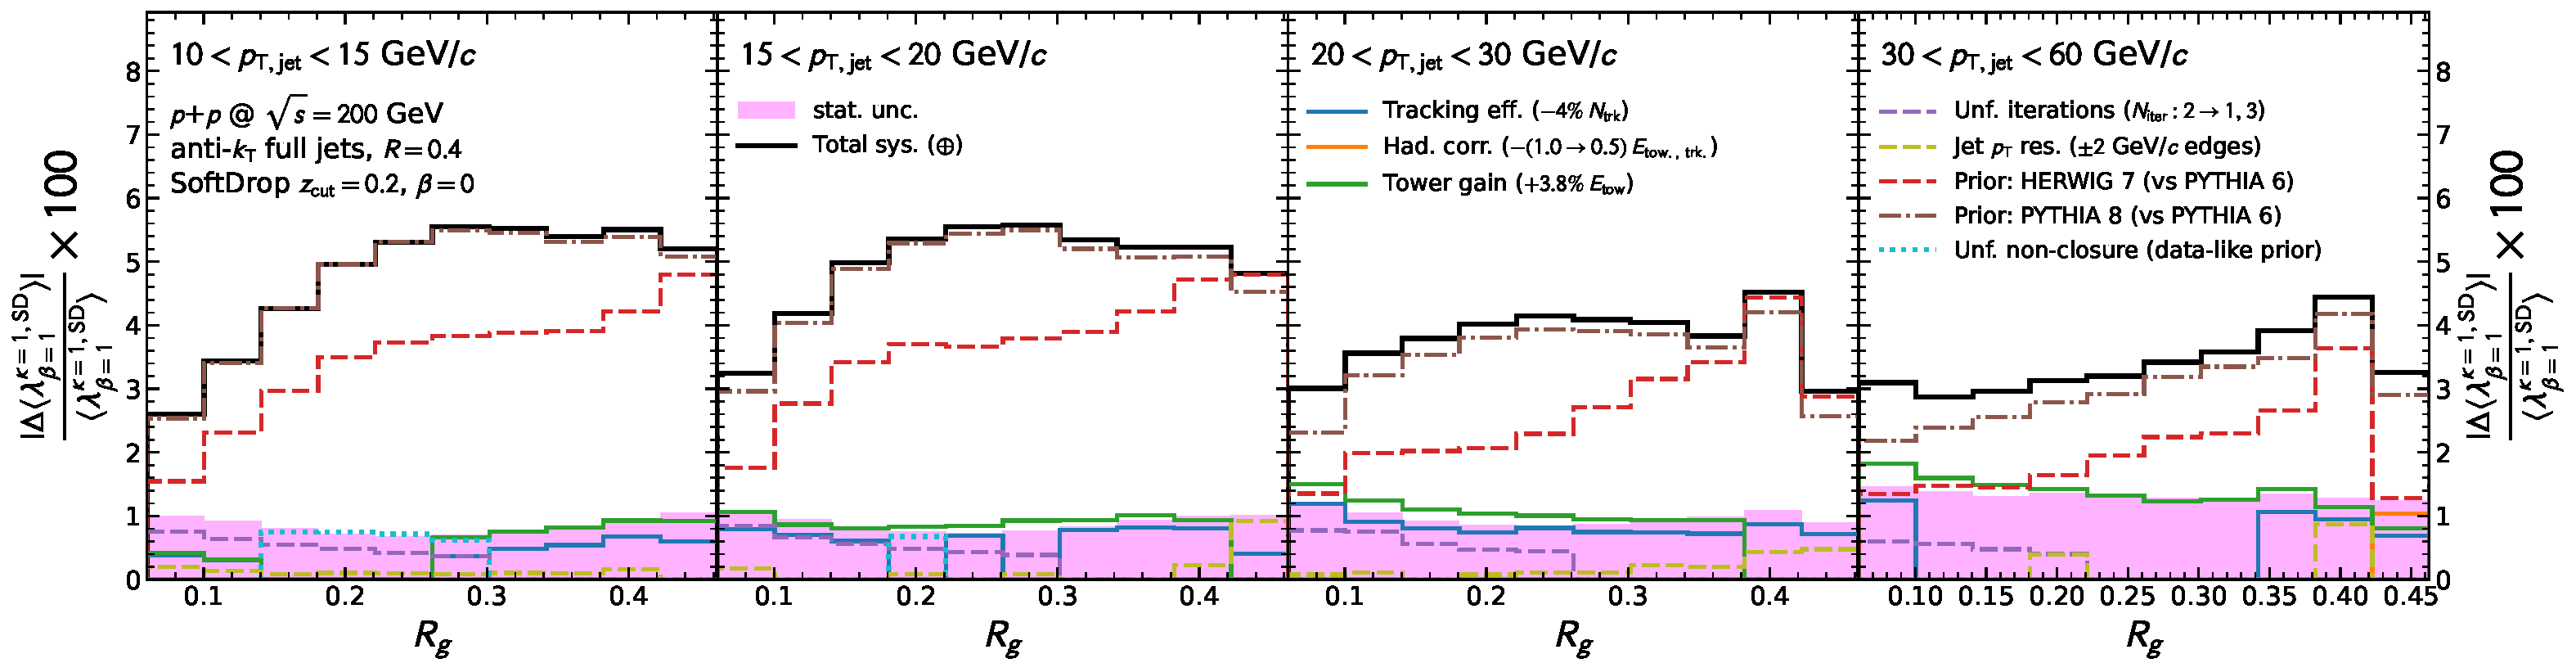
\includegraphics[width=\linewidth]{angularities/pp/sys_ch_ang_k1_b1_prof_sd_vs_sd_dR.pdf}
 	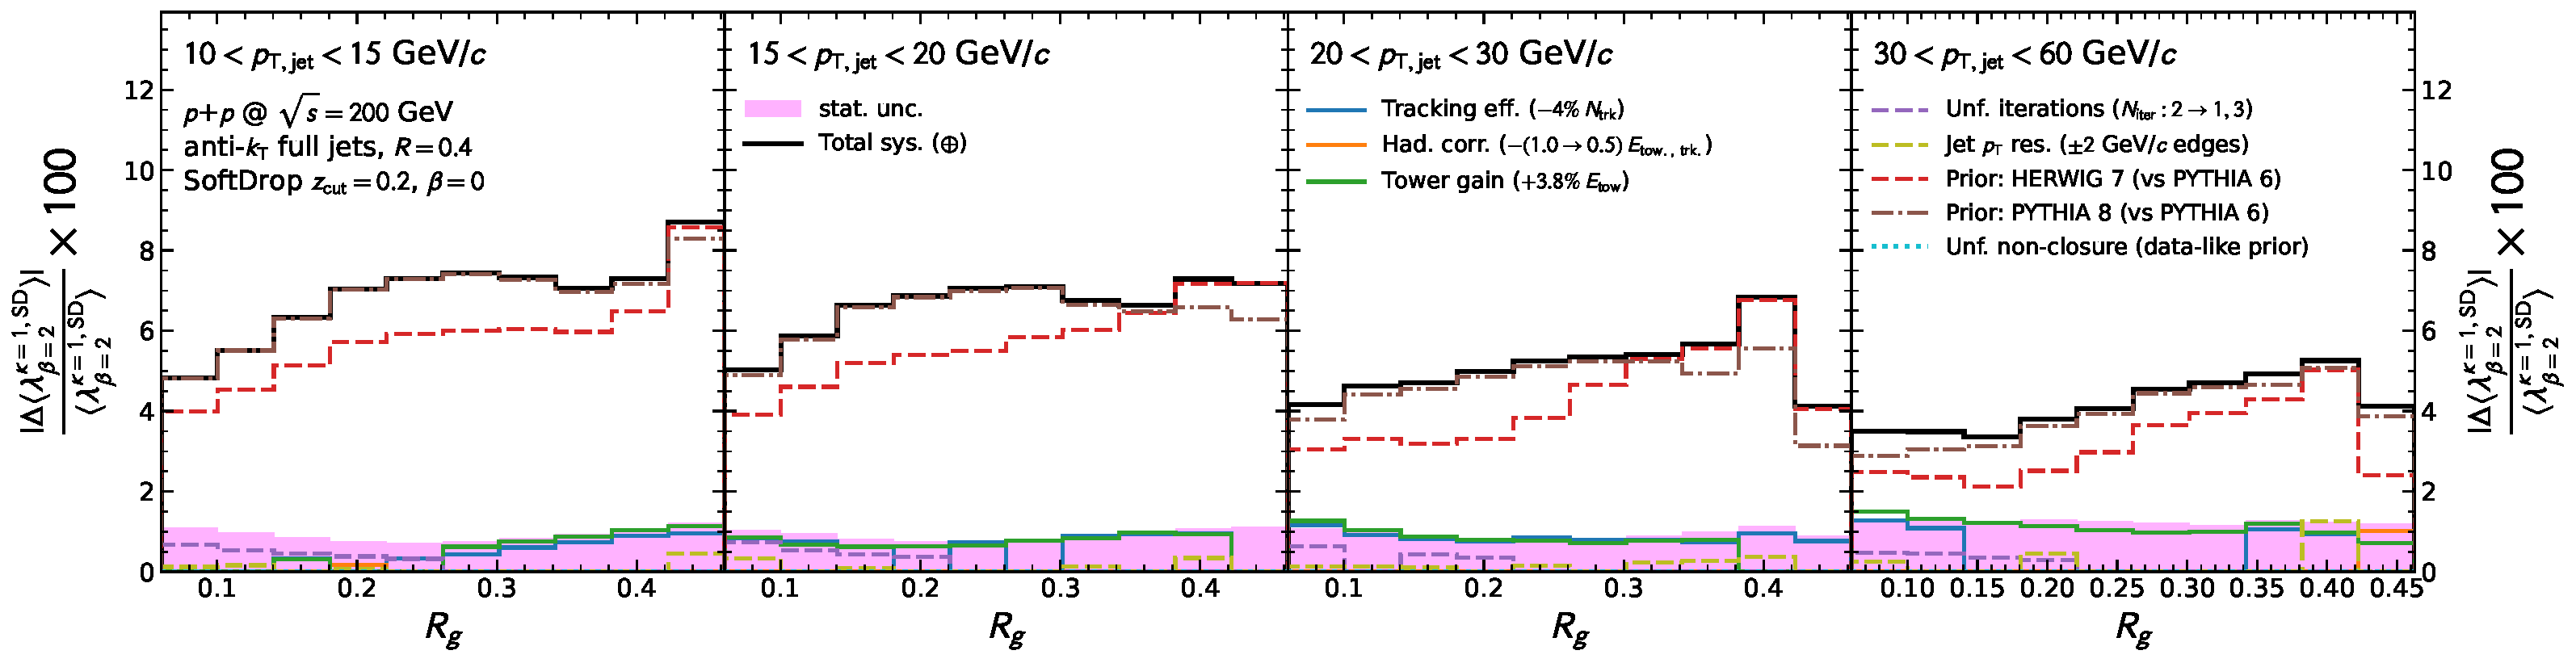
\includegraphics[width=\linewidth]{angularities/pp/sys_ch_ang_k1_b2_prof_sd_vs_sd_dR.pdf}
	\caption{Relative systematic uncertainties of the \(\langle\lambda^{\kappa=1}_{\beta}\rangle\) vs.\ \(R_\mathrm{g}\) profiles of SoftDrop-groomed jets, after the Barlow check (Sec.~\ref{sec:barlow}), for \(\beta = 0.5\), 1 and 2 (top to bottom). The sources are the tracking efficiency, the hadronic correction and the tower gain (solid), the number of unfolding iterations, the jet-\(p_\mathrm{T}\) resolution and the HERWIG-7 and PYTHIA-8 priors (dashed), and the non-closure (dotted); the black line is their sum in quadrature and the magenta band is the statistical uncertainty. Jet-\(p_\mathrm{T}\) ranges are shown as panels.}
	\label{fig:SysProfSD}
\end{figure}
 
 \subsubsection{Barlow check and pruning systematic uncertainties}
 \label{sec:barlow}
 The ensembles of Sec.~\ref{sec:bootstrap} are also used to decide whether a systematic variation is significant. 
 %
 Each variation is a complete unfolding with its own ensemble, giving \(\bar{H}_\mathrm{var.}\) and \(\sigma_\mathrm{var.}\) alongside the nominal \(\bar{H}_\mathrm{nom.}\) and \(\sigma_\mathrm{nom.}\). 
 %
 The shift \(\bar{H}_\mathrm{var.} - \bar{H}_\mathrm{nom.}\) is partly a statistical fluctuation between two ensembles, whose size is estimated as \(\sigma^2_\mathrm{uncorr.} = |\sigma^2_\mathrm{var.} - \sigma^2_\mathrm{nom.}|\), and the shift is only counted as a systematic uncertainty in a bin where
 \begin{equation}
 	\label{eq:barlow}
 	\frac{|\bar{H}_\mathrm{var.} - \bar{H}_\mathrm{nom.}|}{\sigma_\mathrm{uncorr.}} \geq 1 ,
 \end{equation}
 the \emph{Barlow test}, and is set to zero otherwise. 
 
 \subsection{Comparison with published STAR results}
As a cross-check of the unfolding, the jet mass \(M_\mathrm{jet}\) and groomed jet mass \(M_\mathrm{jet, g}\)~\cite{STAR:2021lvw}, and the groomed radius \(R_\mathrm{g}\) and momentum fraction \(z_\mathrm{g}\)~\cite{STAR:2020ejj}, previously measured by STAR in \(p+p\) collisions at \sPP{200}{GeV} with the same jet definition, are calculated from the jets unfolded in this work.
%
They are shown in the \(p_\mathrm{T, jet}\) ranges of the publications, and the groomed observables are obtained by grooming the unfolded jets again with SoftDrop at \(z_\mathrm{cut} = 0.1\), \(\beta = 0\), as in the publications.
%
The systematic uncertainties of this work in these comparisons include the number of iterations, the jet-\(p_\mathrm{T}\) resolution, the HERWIG-7 prior, the non-closure, the tracking efficiency and the hadronic correction.
%
The jet mass, \(R_\mathrm{g}\) and \(z_\mathrm{g}\) of this work agree with the published results within uncertainties in most bins (Fig.~\ref{fig:starpub}), while the groomed mass is higher than the published one in the lowest \(M_\mathrm{jet, g}\) bins.
\begin{sidewaysfigure}
	\centering
	\begin{tabularx}{\linewidth}{XX}
		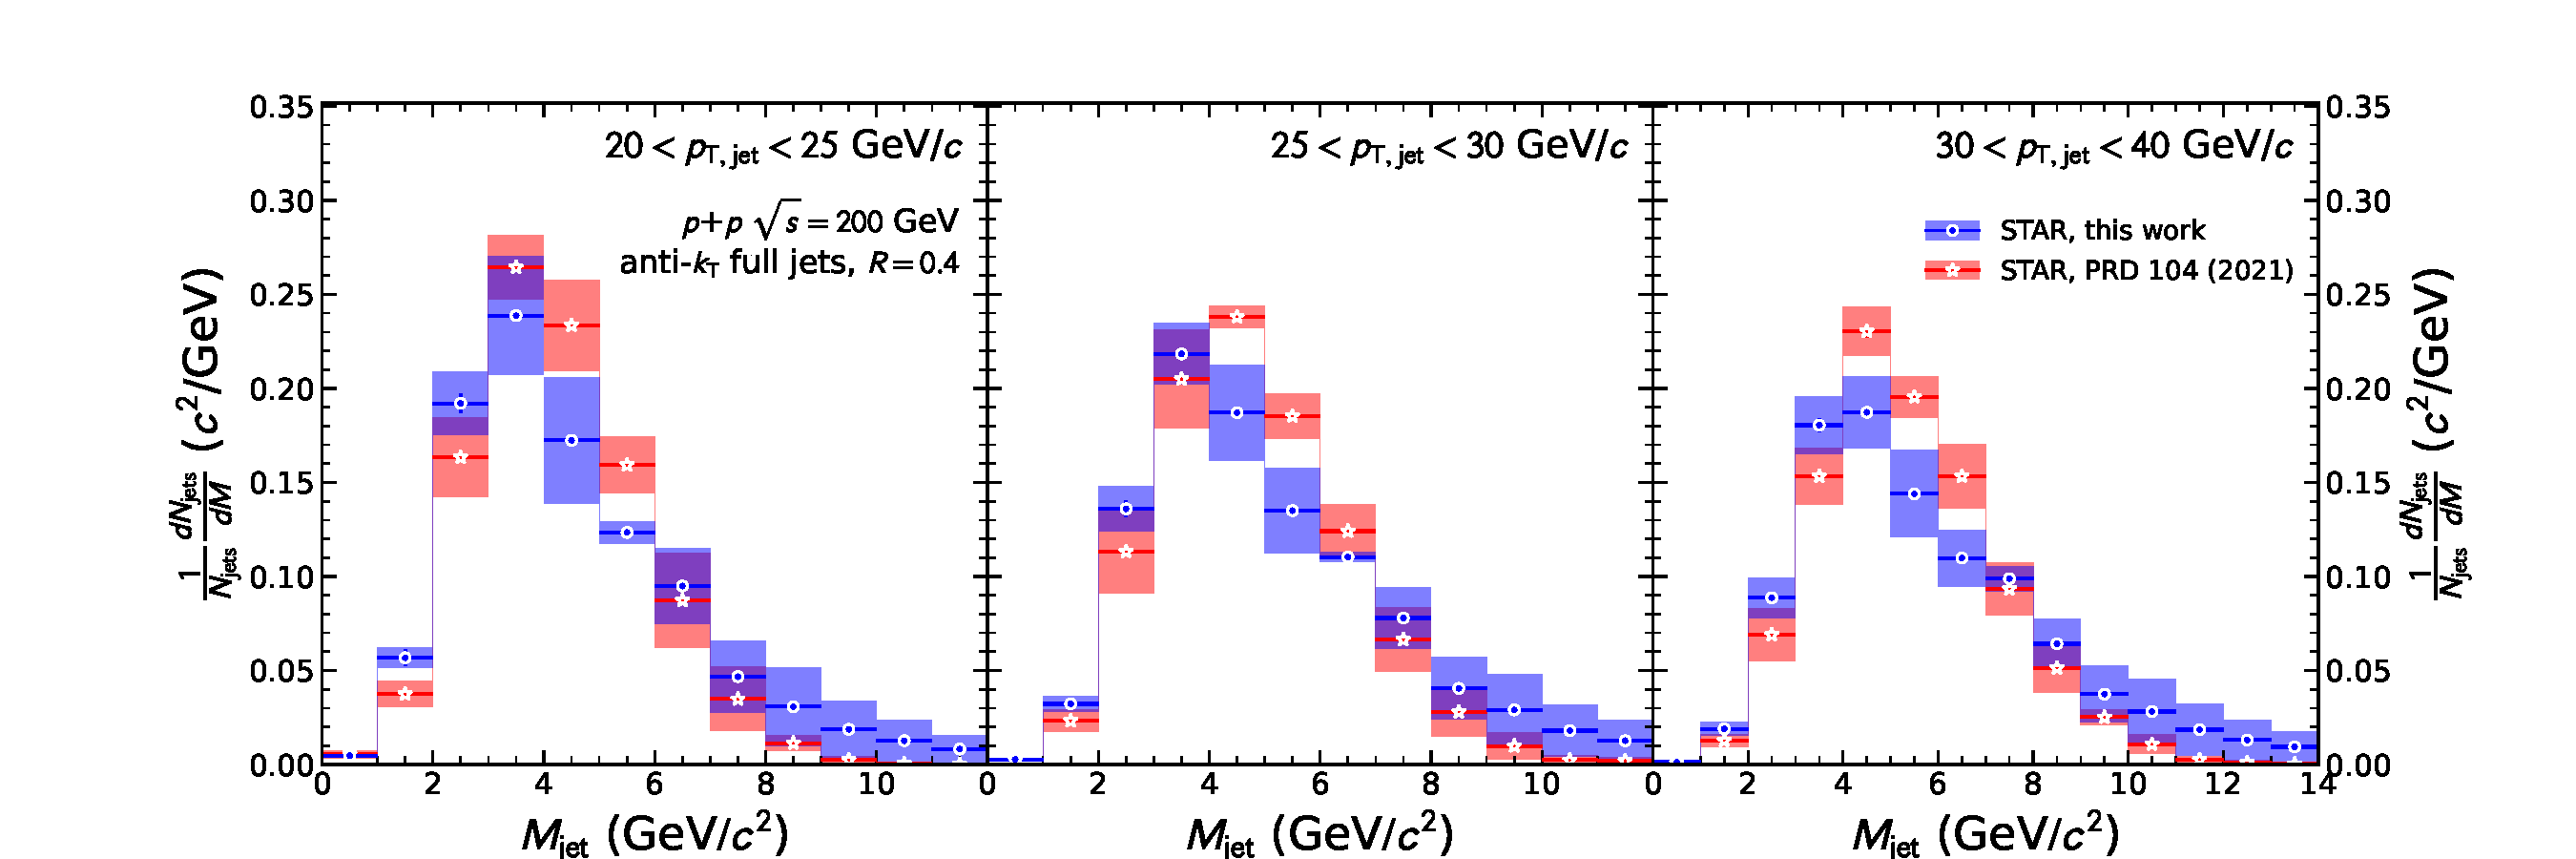
\includegraphics[width=\linewidth]{figures/angularities/pp/pub_comparison/star_published/star_pub_m} &
		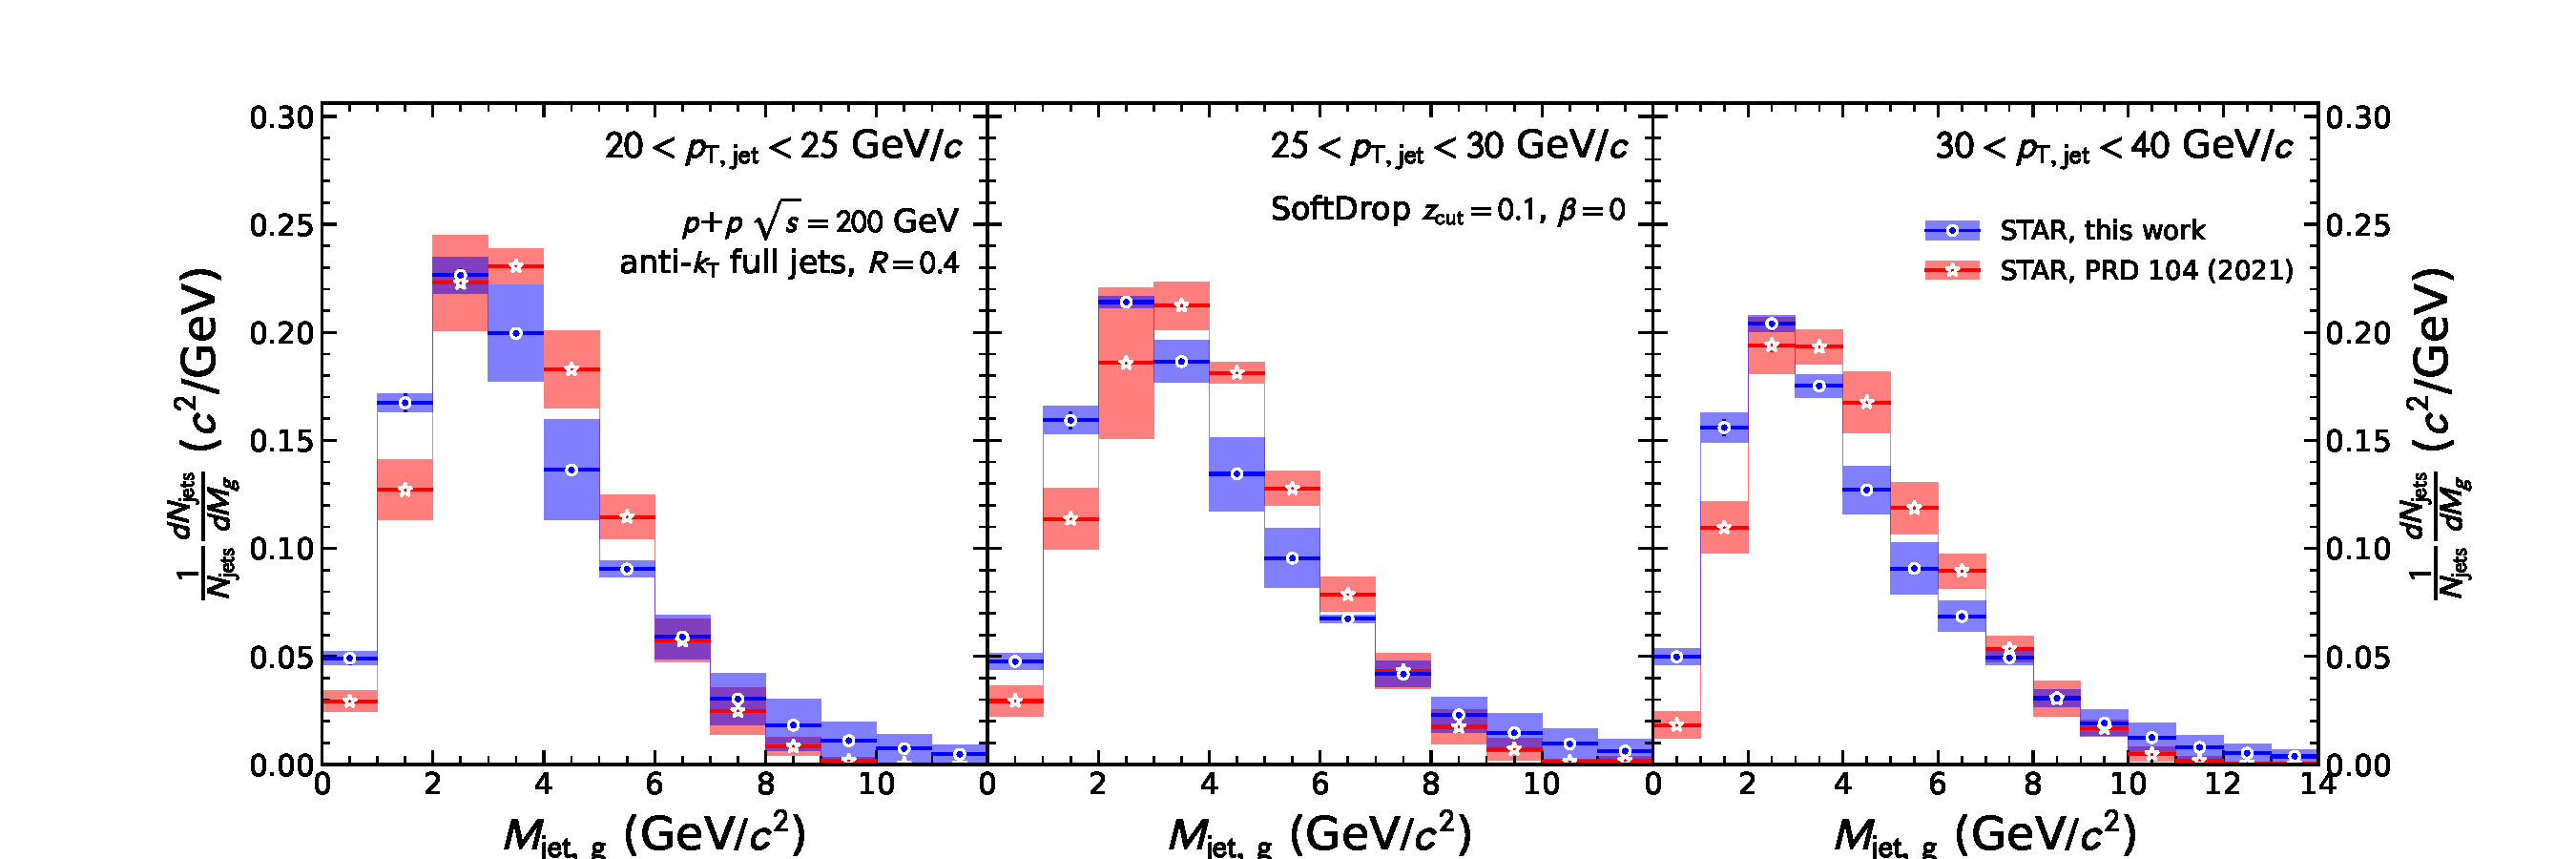
\includegraphics[width=\linewidth]{figures/angularities/pp/pub_comparison/star_published/star_pub_sd_m} \\
		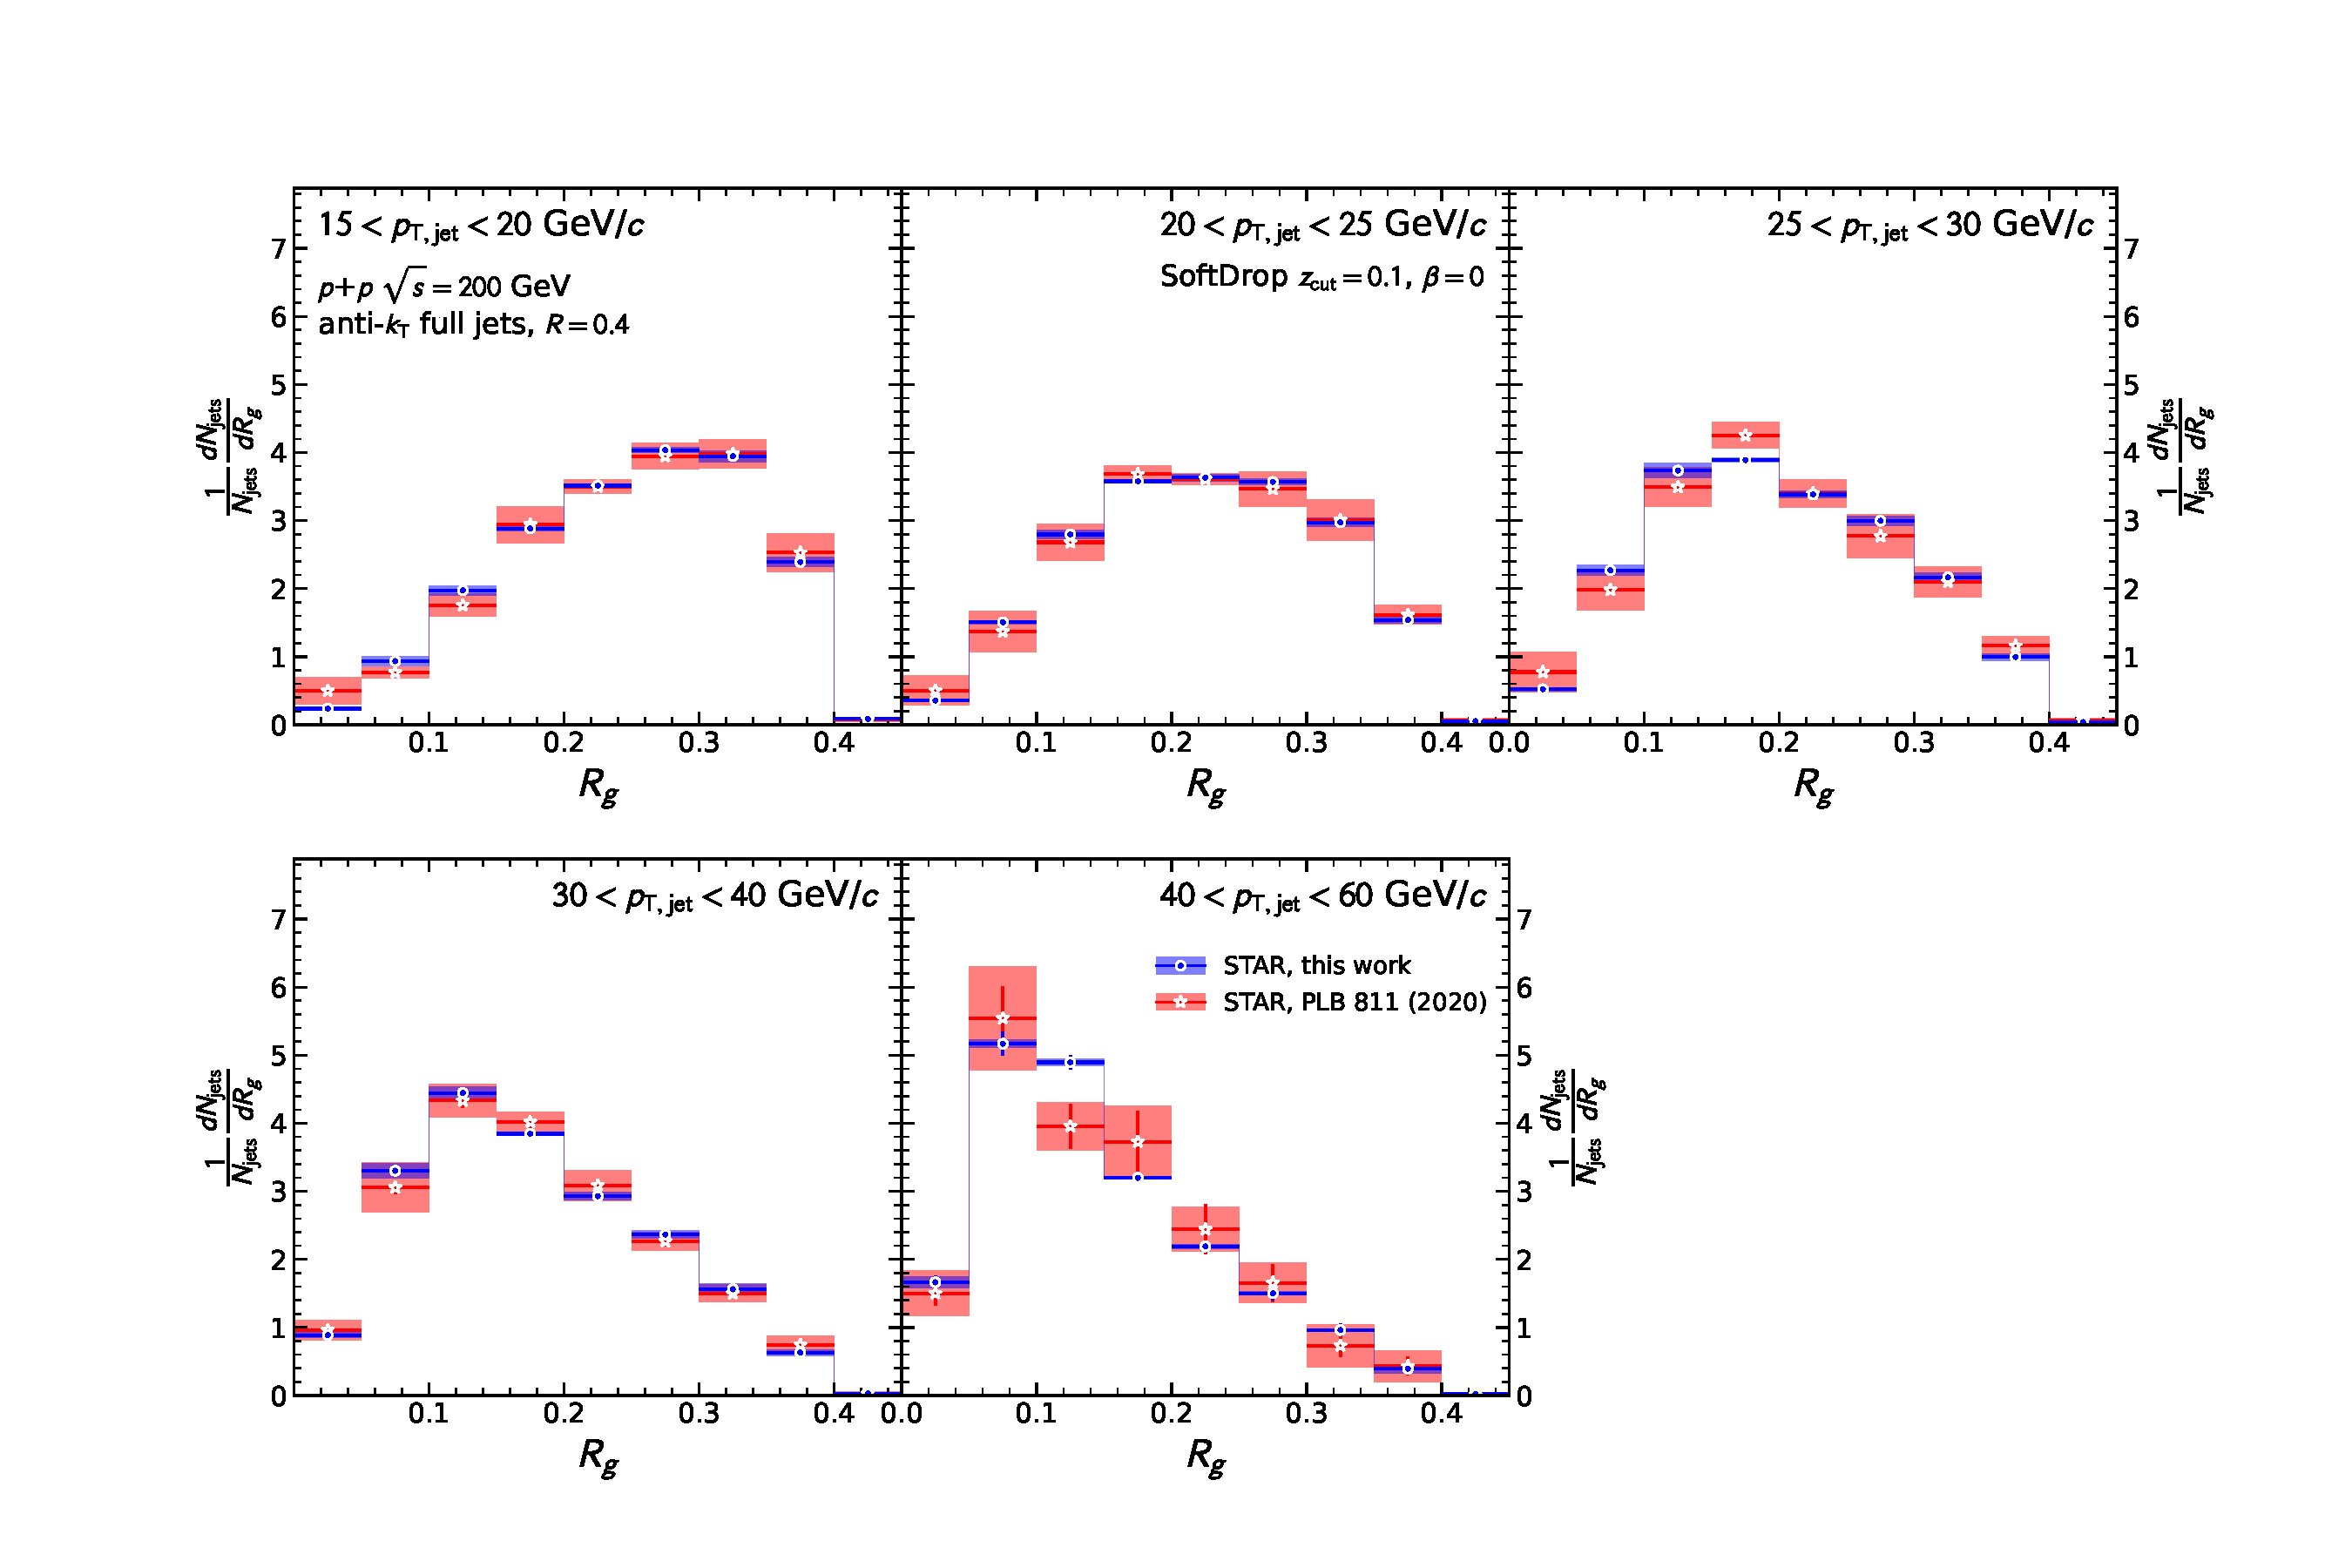
\includegraphics[width=\linewidth]{figures/angularities/pp/pub_comparison/star_published/star_pub_sd_dR} &
		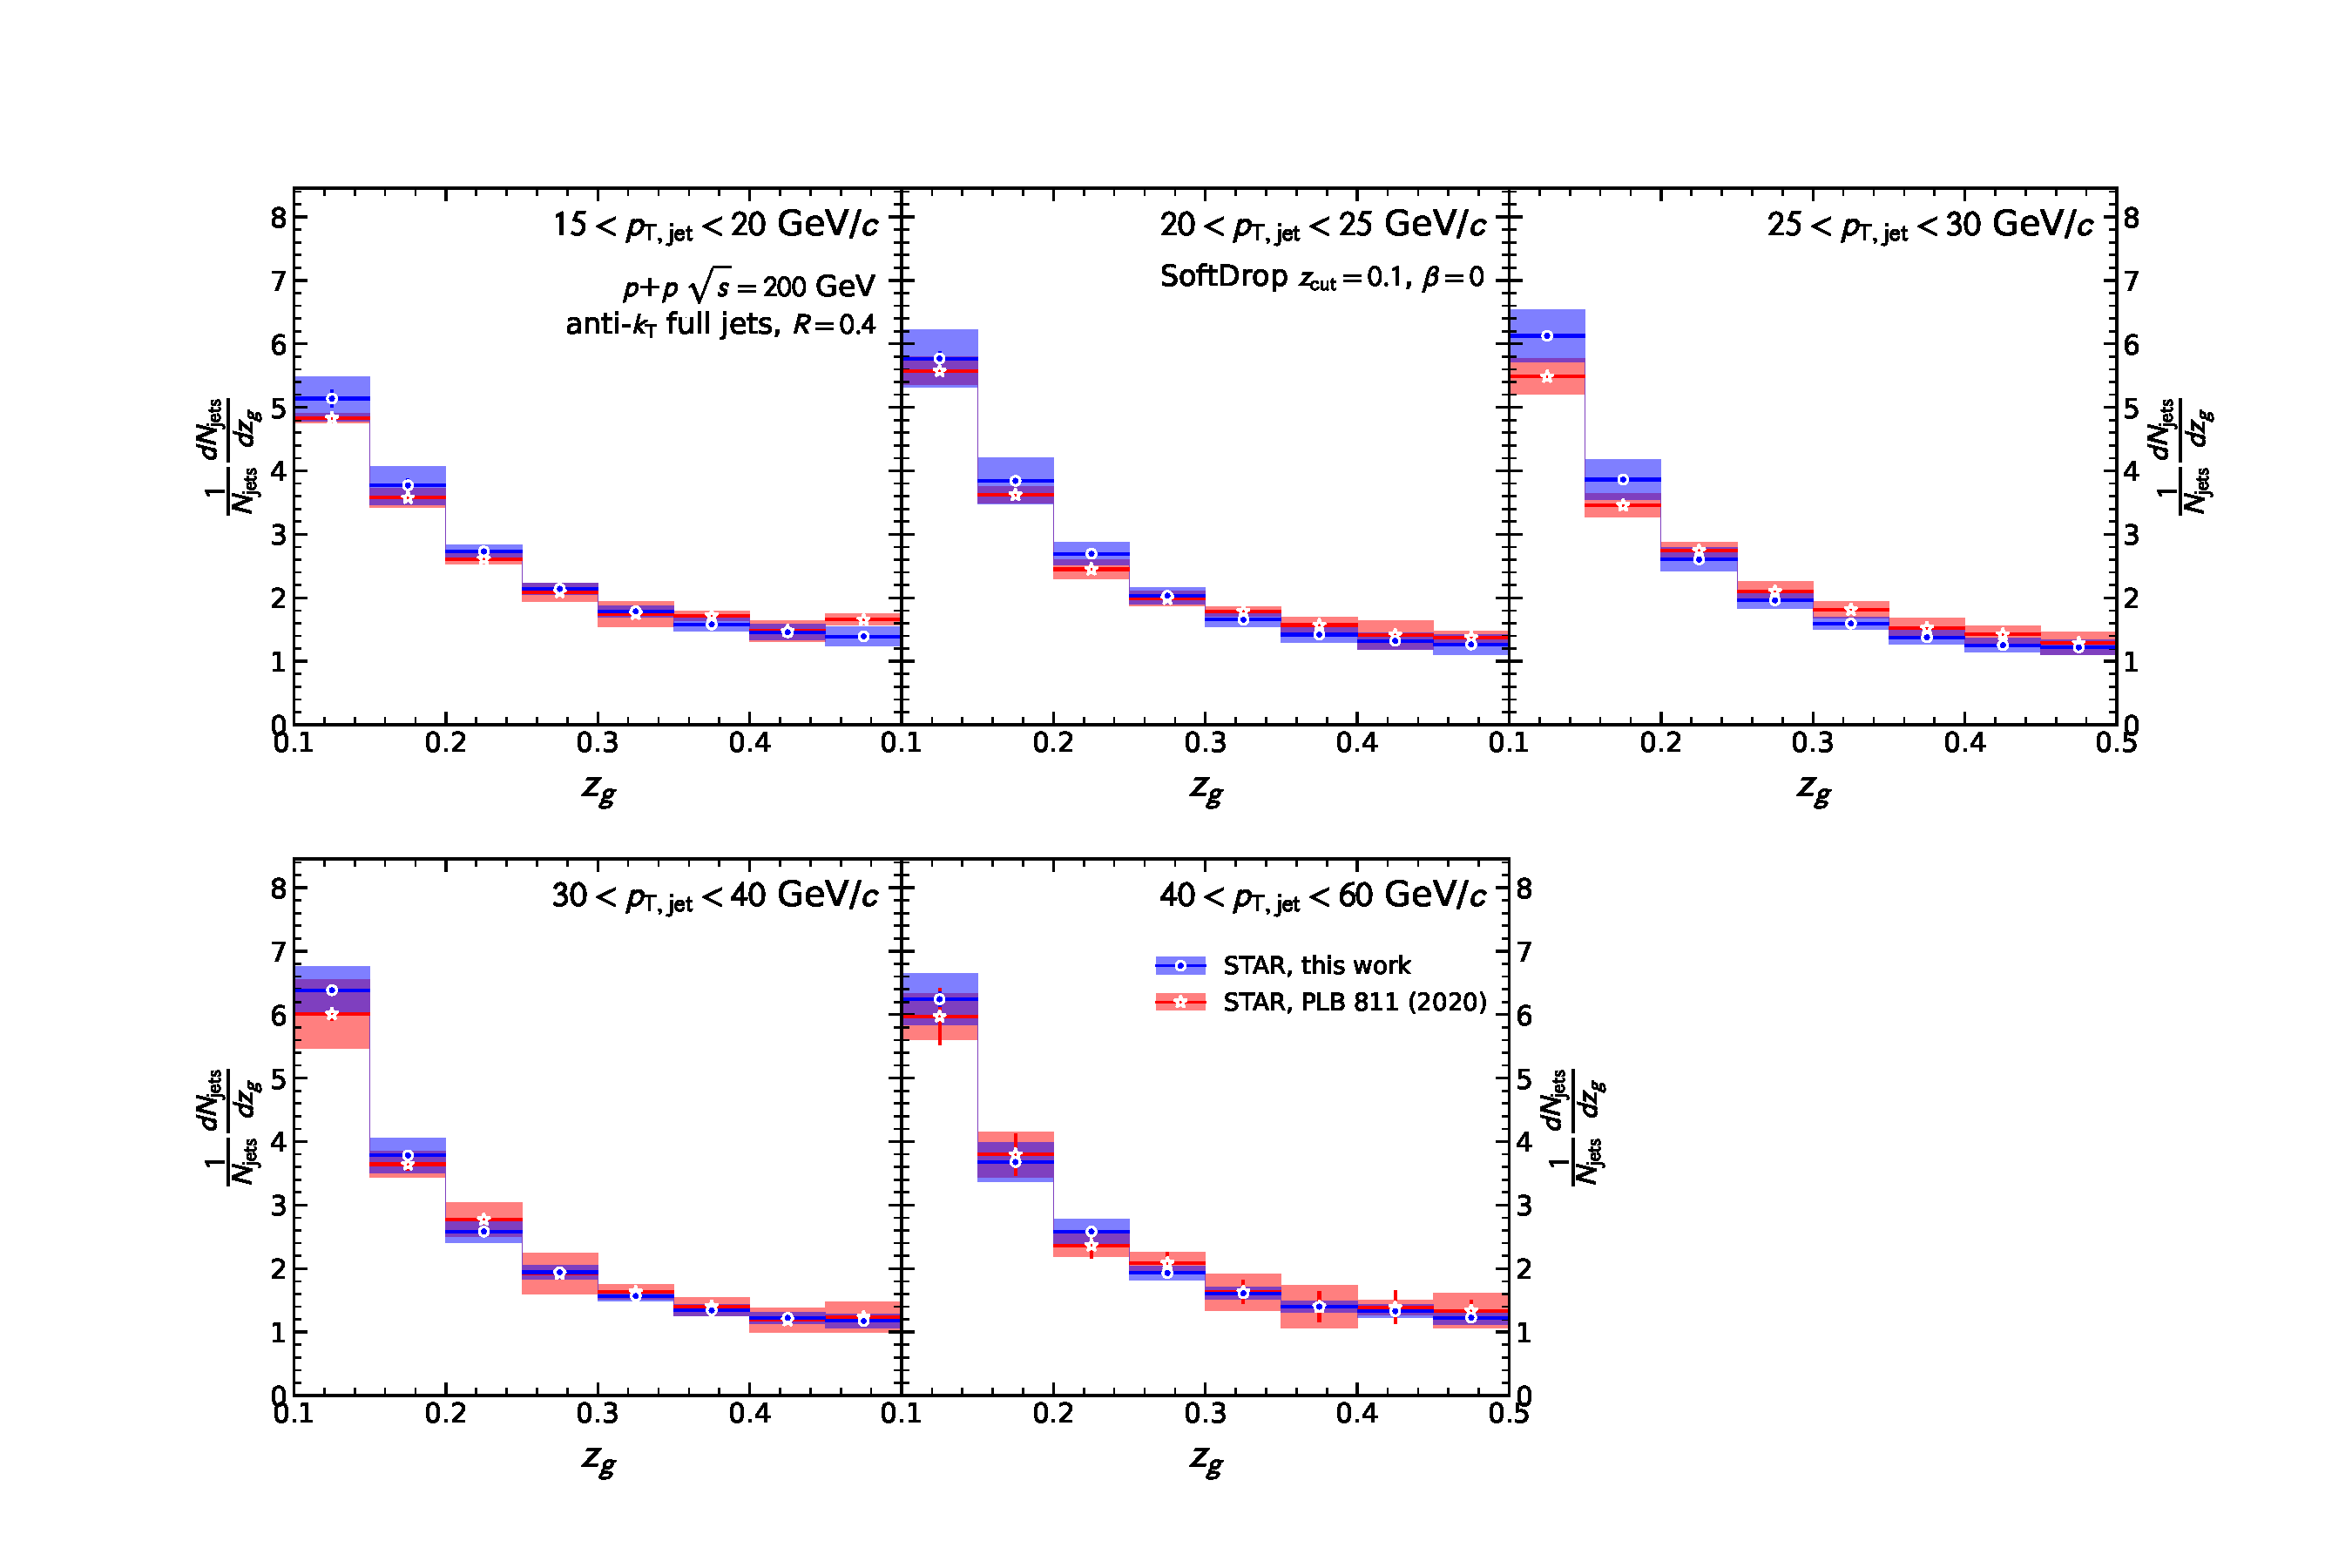
\includegraphics[width=\linewidth]{figures/angularities/pp/pub_comparison/star_published/star_pub_sd_symmetry} \\
	\end{tabularx}
	\caption{Comparison of this work (blue), obtained from the same unfolded jets, with published STAR measurements (red) in \(p+p\) collisions at \sPP{200}{GeV}, in their \(p_\mathrm{T, jet}\) ranges. (Top) Jet mass \(M_\mathrm{jet}\) (left) and groomed jet mass \(M_\mathrm{jet, g}\) (right) compared to Ref.~\cite{STAR:2021lvw}. (Bottom) Groomed radius \(R_\mathrm{g}\) (left) and groomed momentum fraction \(z_\mathrm{g}\) (right) compared to Ref.~\cite{STAR:2020ejj}. The groomed observables use SoftDrop with \(z_\mathrm{cut} = 0.1\), \(\beta = 0\), as in the publications. Boxes show the systematic and bars the statistical uncertainties.}
	\label{fig:starpub}
\end{sidewaysfigure}
 
\subsection{Results and Discussions}
\label{sec:ppResults}
\paragraph{Distributions.}
The unfolded \(\lambda_{\beta}^{\kappa=1}\) distributions for \(\beta = 0.5\) (LHA), 1 (girth) and 2 (thrust) are shown in Fig.~\ref{fig:ppDist} for inclusive and SoftDrop-groomed jets in the three \(p_\mathrm{T, jet}\) ranges.
%
With increasing \(p_\mathrm{T, jet}\) all distributions become narrower and move to smaller values; the peak of the inclusive girth distribution, for example, moves from about 0.18 to about 0.11 between the lowest and the highest \(p_\mathrm{T, jet}\) range.
%
This is the expected behavior of collinear radiation, whose angular spread decreases as the jet energy grows.

Grooming shifts all distributions to smaller angularity values, since the soft, wide-angle constituents it removes contribute the most to \(\lambda_\beta\).
%
The change of shape grows with \(\beta\), because a larger \(\beta\) weights the constituents far from the axis more strongly: for \(\beta = 0.5\) the groomed distribution is a moderately shifted version of the inclusive one, while for \(\beta = 2\) the groomed thrust falls steeply from the smallest values, most of the groomed jets being reduced to a narrow core.

PYTHIA-6, PYTHIA-8 and HERWIG-7 reproduce the overall shape and the \(p_\mathrm{T, jet}\) and \(\beta\) dependence of the data, but all three predict jets that are narrower than measured: they overshoot the data at small \(\lambda_\beta\), most visibly for the LHA, and undershoot the large-\(\lambda_\beta\) tails.
%
The deficit in the tails reaches 20--40\% for HERWIG-7 and PYTHIA-8, beyond the systematic uncertainties, while PYTHIA-6 stays within them in most bins, for both inclusive and groomed jets.
%
For \(\beta = 1\) and 2, grooming reduces the deviations of HERWIG-7 and PYTHIA-8 from the data, most clearly at higher \(p_\mathrm{T, jet}\), consistent with the removal of the soft wide-angle radiation that is most sensitive to the hadronization modelling; PYTHIA-6 does not show this improvement.
%
Since PYTHIA-6 is also the prior of the unfolding, this agreement alone does not prove a good description, but the prior variations to HERWIG-7 and PYTHIA-8 (Sect.~\ref{sec:priorReweighting}) are part of the systematic uncertainty, so a result pulled towards the prior would show up there.

\paragraph{Angularities as functions of the groomed radius.}
The unbinned unfolding provides the full set of jet features for every jet, so that any observable can be projected afterward without being chosen, or binned, before the unfolding.
%
This is used here to measure the mean angularities as a function of the SoftDrop groomed radius, \(\langle\lambda^{\kappa=1}_\beta\rangle\) vs \(R_\mathrm{g}\), shown in Fig.~\ref{fig:ppProfRg}, which correlates the radiation pattern of the whole jet with the angle of its first hard splitting.

\(\langle\lambda^{\kappa=1}_\beta\rangle\) rises monotonically with \(R_\mathrm{g}\) for all \(\beta\), for both inclusive and groomed jets.
%
For the groomed jets, all constituents lie roughly within \(R_\mathrm{g}\) of the axis, so \(\langle\lambda_\beta\rangle\) grows approximately as \(R_\mathrm{g}^\beta\): the rise is concave for \(\beta = 0.5\), close to linear for \(\beta = 1\) and convex for \(\beta = 2\).
%
The inclusive values lie above the groomed ones by the contribution of the soft radiation removed by the grooming, and the two converge at large \(R_\mathrm{g}\).
%
This reflects the angular ordering of the clustering sequence: a jet with a large \(R_\mathrm{g}\) has its widest splitting already passing the SoftDrop condition, so almost nothing is groomed away, while a small \(R_\mathrm{g}\) means that wide-angle soft branches were removed before the first hard splitting was found.
%
At fixed \(R_\mathrm{g}\) the mean angularities depend only weakly on \(p_\mathrm{T, jet}\), decreasing by a few percent between the lowest and the highest \(p_\mathrm{T, jet}\) range; most of the narrowing of the distributions with \(p_\mathrm{T, jet}\) seen in Fig.~\ref{fig:ppDist} therefore comes from the shift of the \(R_\mathrm{g}\) distribution towards smaller angles.

The profiles separate the two possible origins of the model deviations seen in the distributions.
%
PYTHIA-6 describes the profiles within uncertainties, but HERWIG-7 and PYTHIA-8 lie 10--15\% below the data at all \(R_\mathrm{g}\), for all \(\beta\), in all \(p_\mathrm{T, jet}\) ranges and for inclusive as well as groomed jets.
%
Their narrower jets are thus not caused by a different distribution of the first splitting angle, but by too little radiation at a given splitting angle, which is information that the one-dimensional distributions alone cannot provide.

\paragraph{Comparison with ALICE.}
Fig.~\ref{fig:aliceComp} compares the \(\lambda^{\kappa=1}_{1}\) and \(\lambda^{\kappa=1}_{2}\) distributions to the ALICE measurement in \(p+p\) collisions at \(\sqrt{s} = 5.02\) TeV~\cite{ALICE:2021njq}, for charged-particle jets with \(20 < p_\mathrm{T, jet}^\mathrm{ch.} < 40\) GeV/\(c\), which are reconstructed from the unfolded jets of this work for the comparison.
%
The charged-jet and full-jet versions of this work agree closely with each other.
%
At the same charged-jet \(p_\mathrm{T}\), the jets at \sPP{200}{GeV} are considerably narrower than at \(\sqrt{s} = 5.02\) TeV, both with and without grooming, as expected from the larger fraction of quark-initiated jets at the lower collision energy.

\paragraph{Summary.}
In terms of the three goals set out at the beginning of this section: the inclusive and groomed angularities, their \(p_\mathrm{T, jet}\) dependence and their correlation with \(R_\mathrm{g}\) provide a \(p+p\) baseline for future measurements in heavy-ion collisions at the same energy; the unbinned unfolding passes its closure tests and reproduces earlier STAR measurements of other observables from the same jets (Fig.~\ref{fig:starpub}); and the \(R_\mathrm{g}\) profiles, obtained from the same unfolding without a dedicated analysis, trace the deviations of HERWIG-7 and PYTHIA-8 from the data to the radiation at a given splitting angle.

\begin{figure}[h]
	\centering
	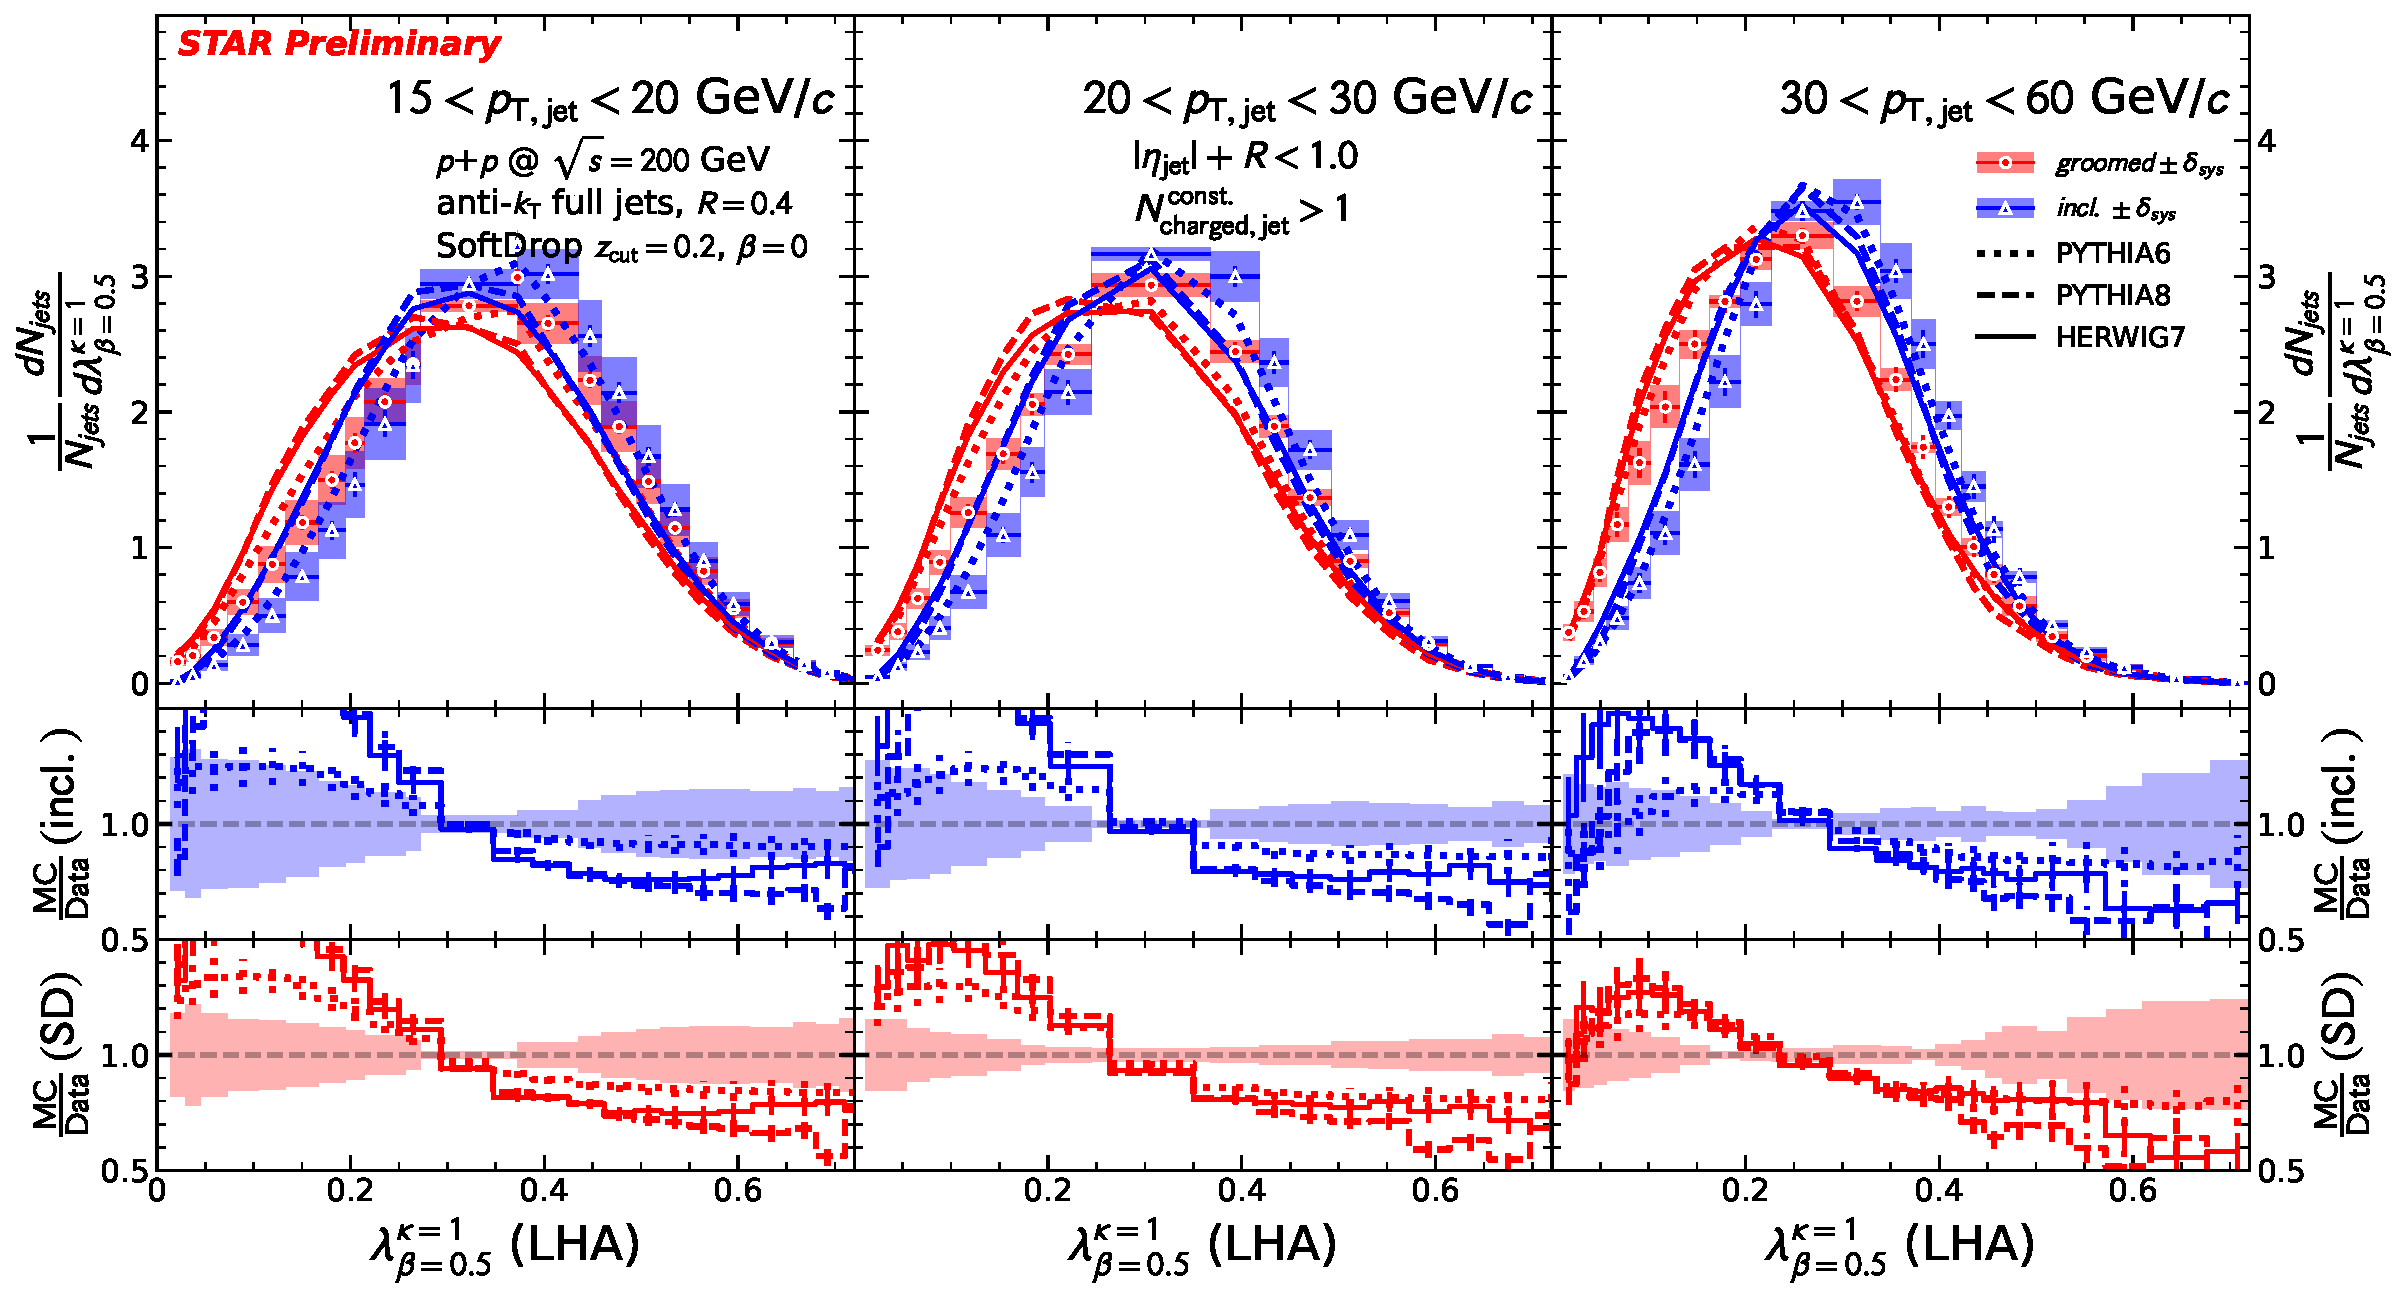
\includegraphics[width=0.9\linewidth]{angularities/pp/fig_dist_ptbins_ch_ang_k1_b0_5.pdf}
	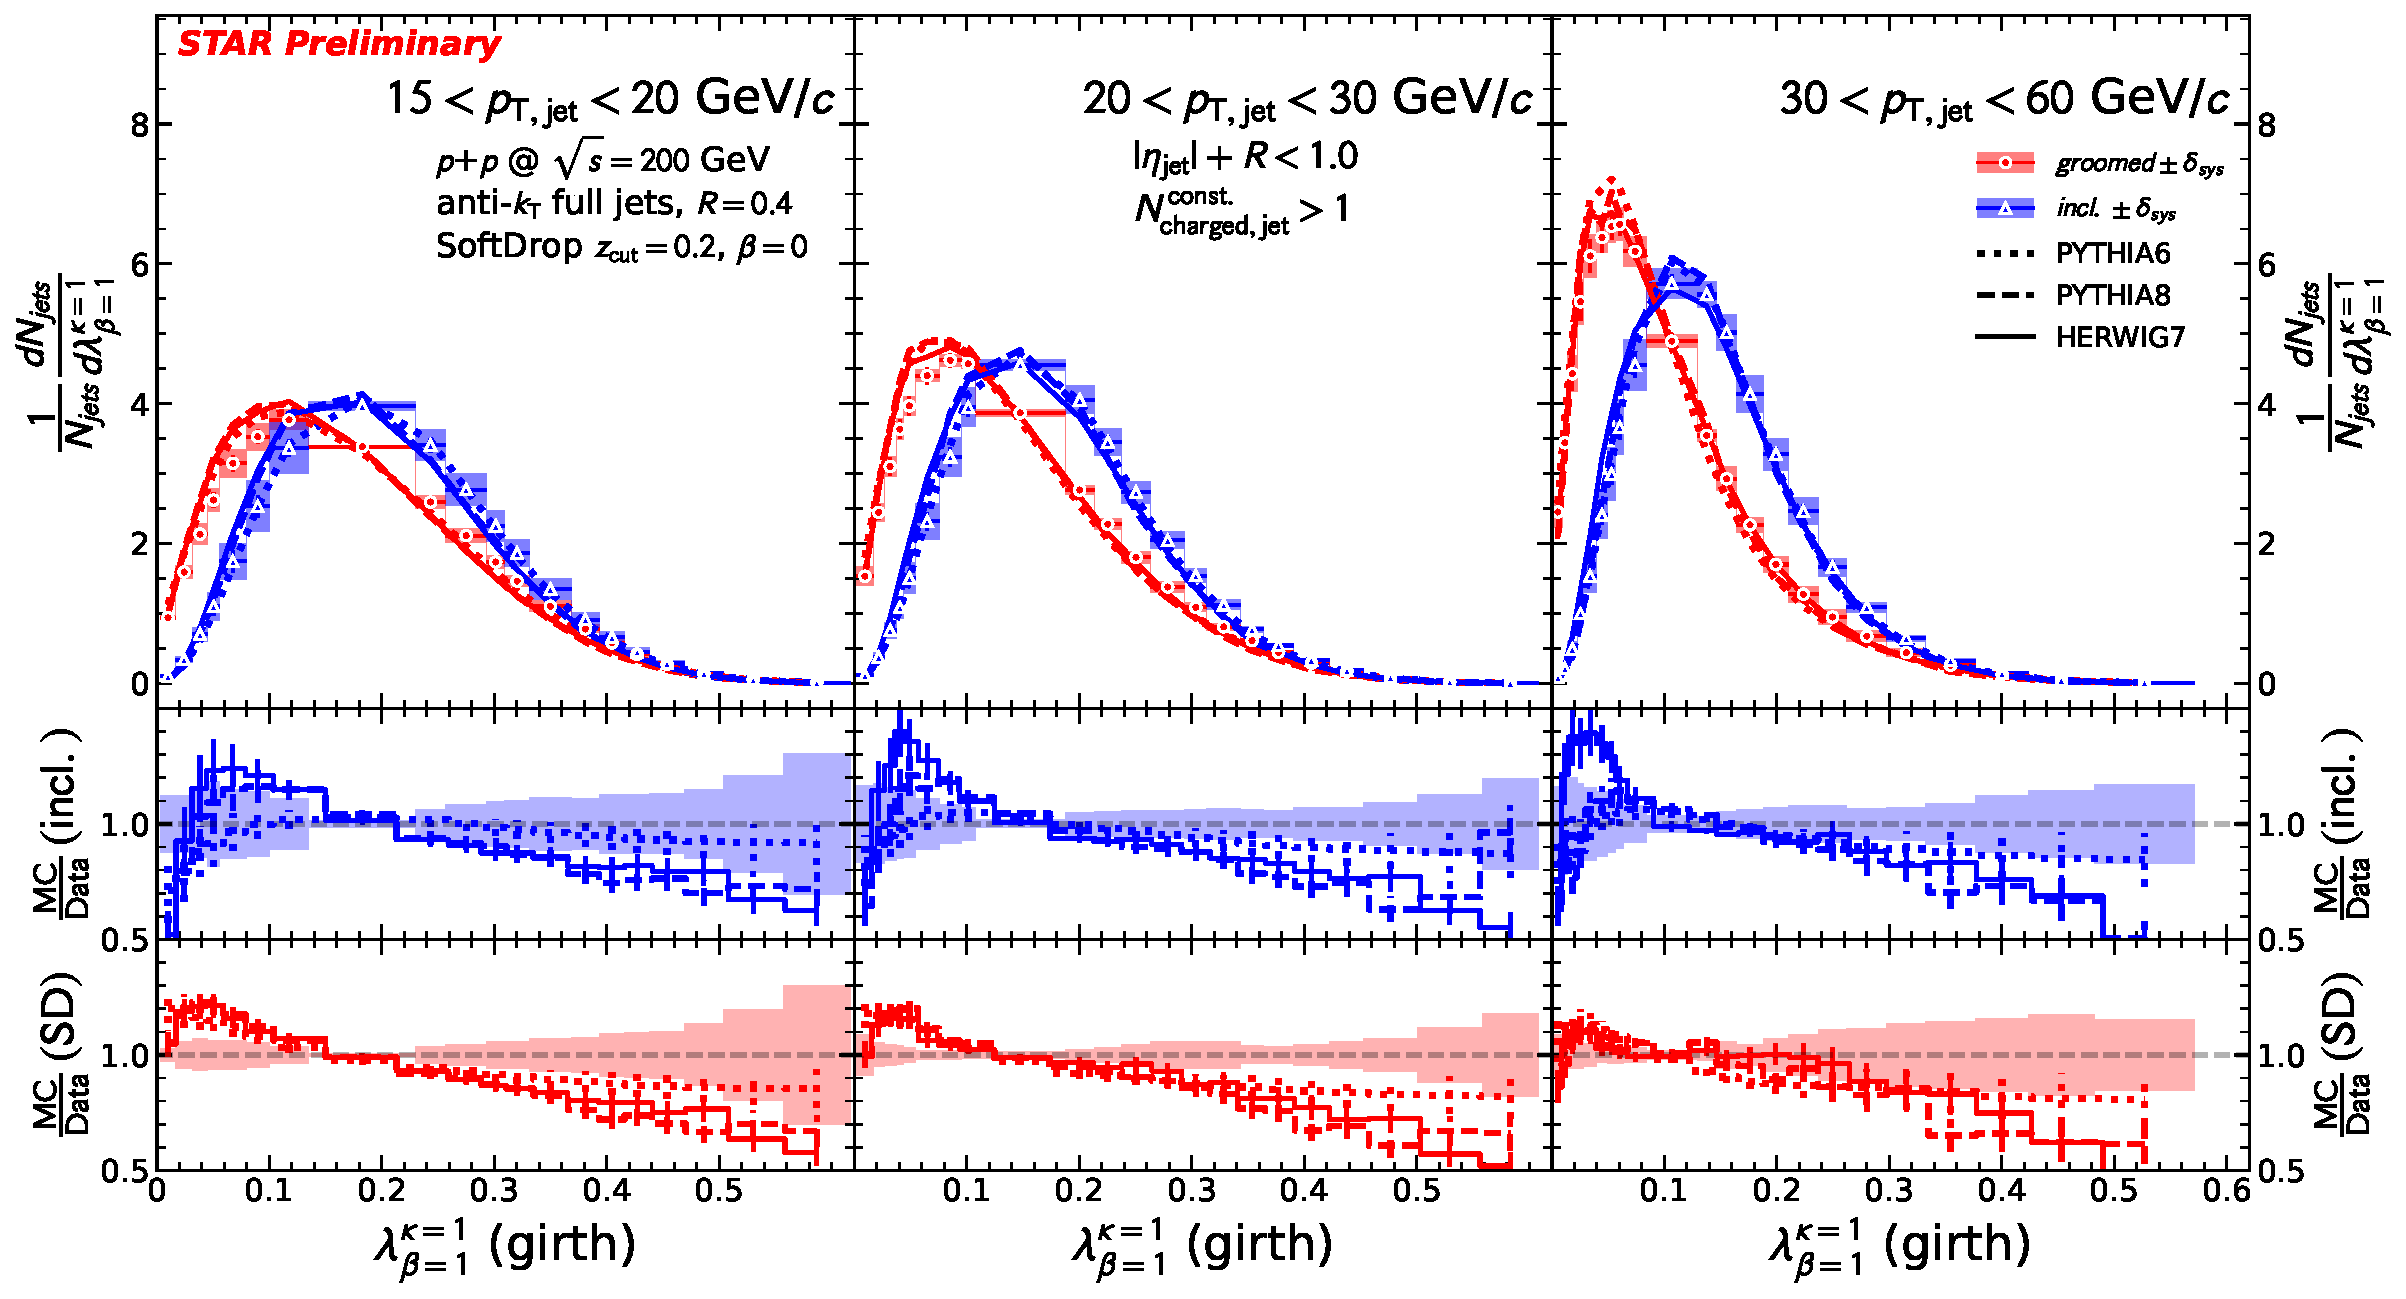
\includegraphics[width=0.9\linewidth]{angularities/pp/fig_dist_ptbins_ch_ang_k1_b1.pdf}
	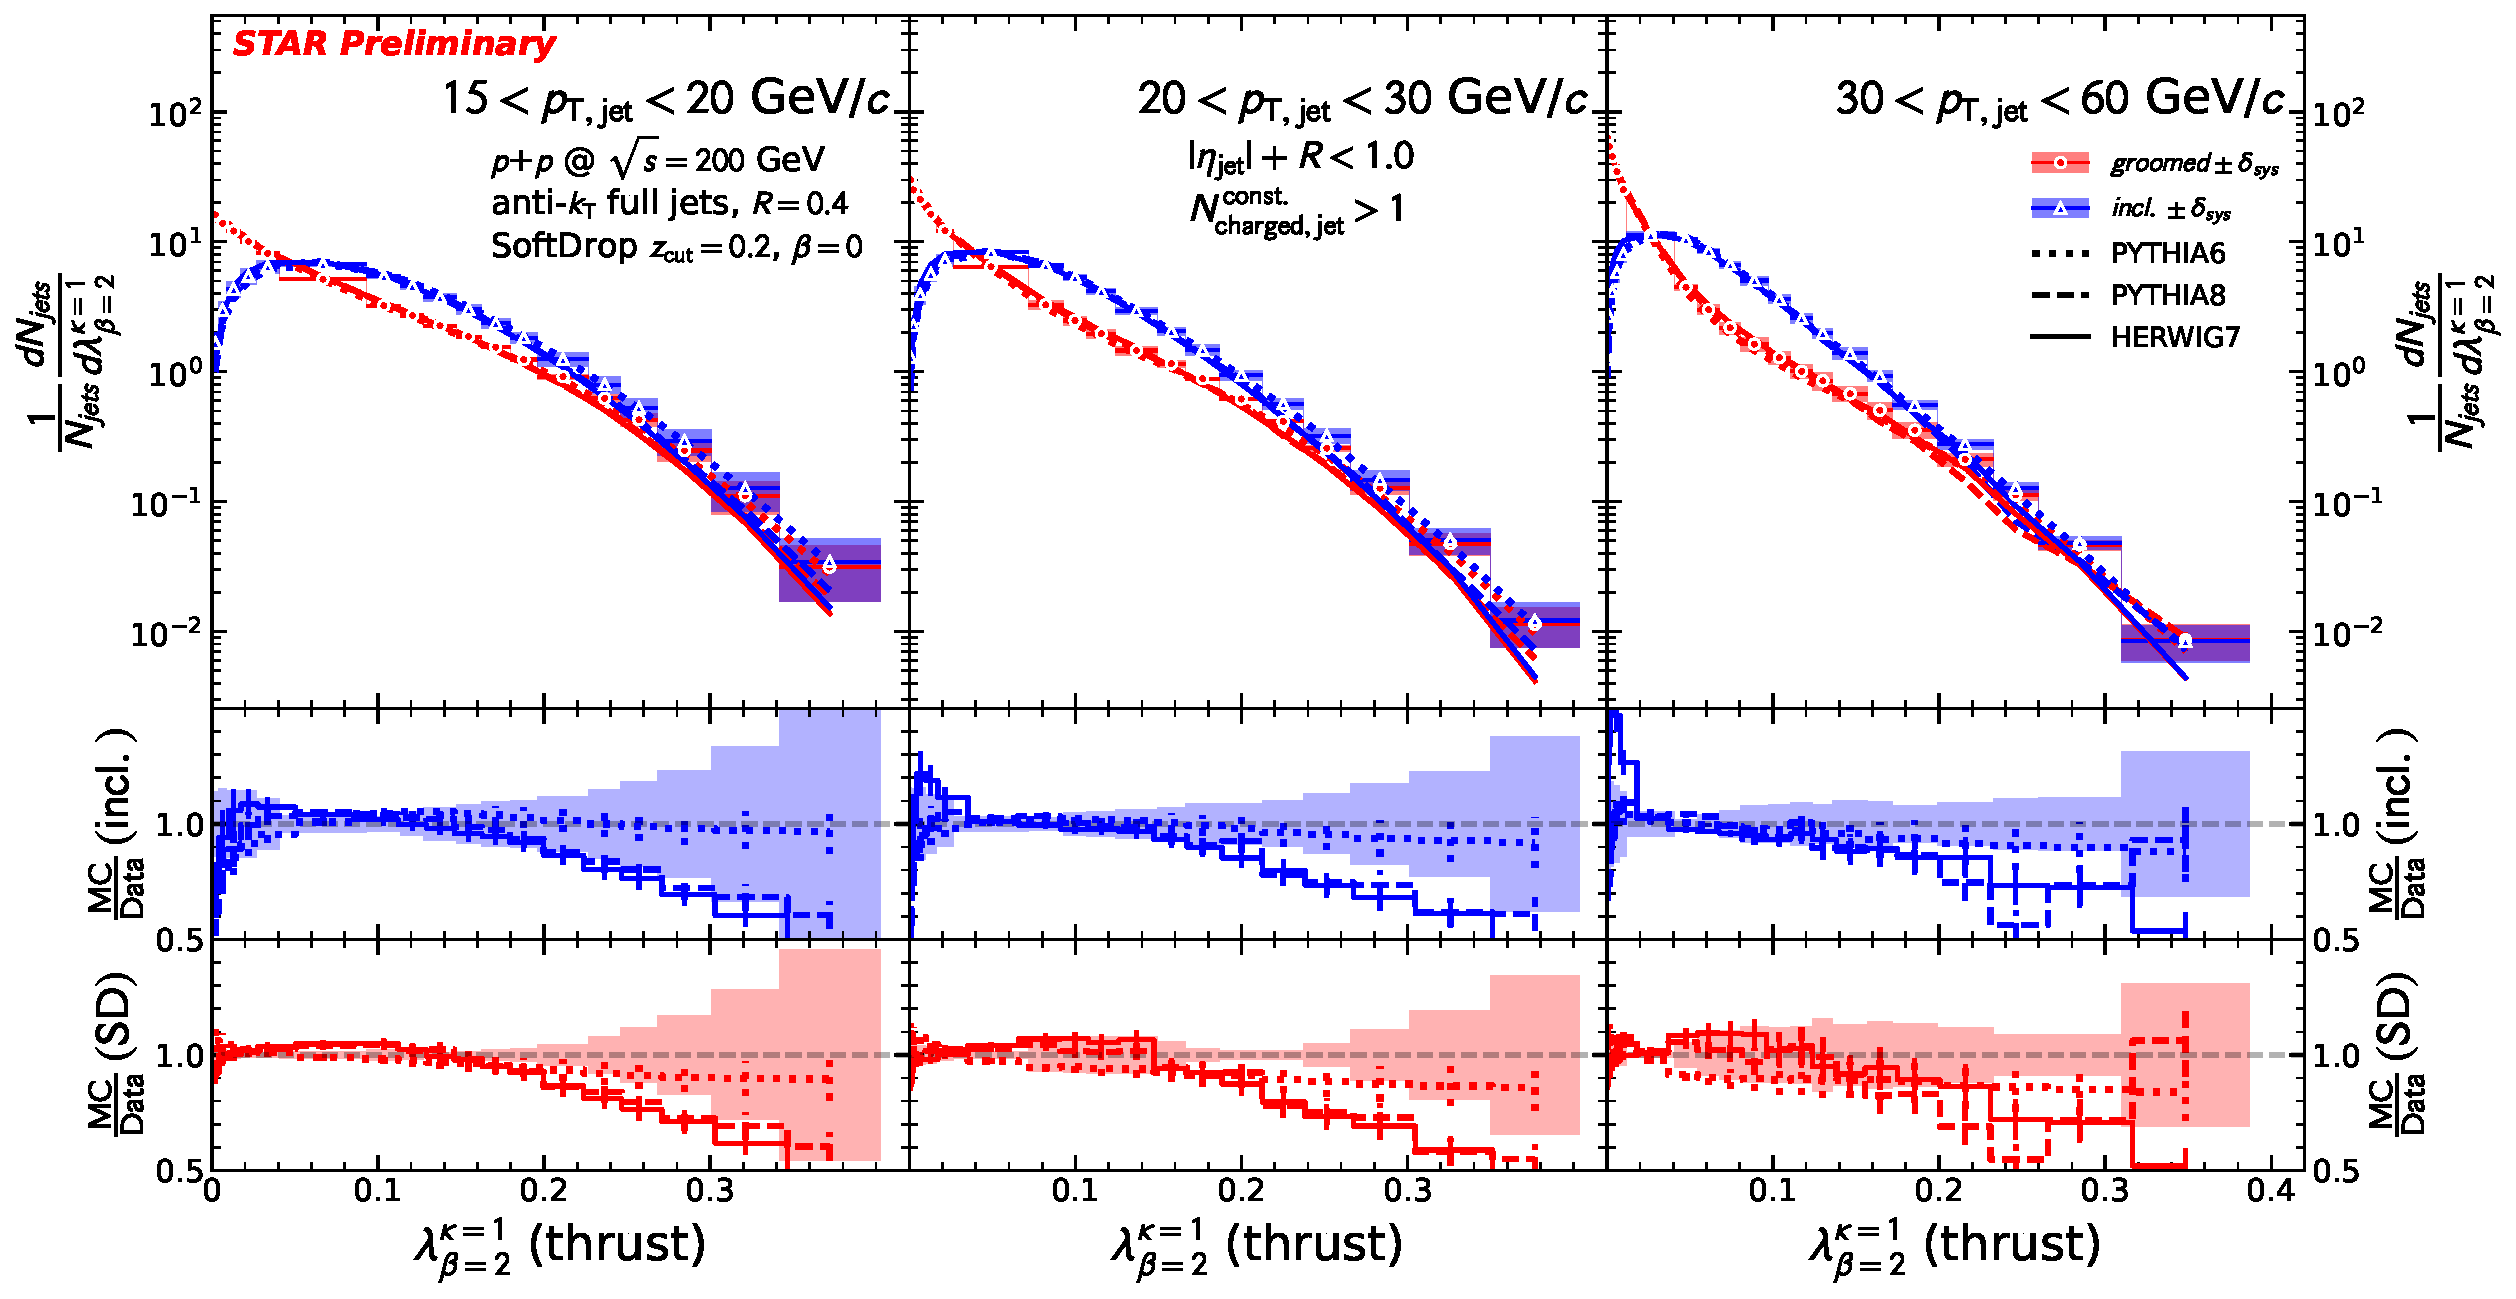
\includegraphics[width=0.9\linewidth]{angularities/pp/fig_dist_ptbins_ch_ang_k1_b2.pdf}
	\caption{Unfolded distributions of \(\lambda^{\kappa=1}_{\beta}\) for \(\beta = 0.5\), 1 and 2 (top to bottom) for inclusive (blue) and SoftDrop-groomed (red, \(z_\mathrm{cut} = 0.2\), \(\beta = 0\)) jets in \(p+p\) collisions at \sPP{200}{GeV}, in three \(p_\mathrm{T, jet}\) ranges (columns). Boxes show the systematic and bars the statistical uncertainties. The measurements are compared to PYTHIA-6 (dotted), PYTHIA-8 (dashed) and HERWIG-7 (solid), and the lower panels show the ratios of the event generators to the data for inclusive and groomed jets, with the relative systematic uncertainty of the data as a band.}
	\label{fig:ppDist}
\end{figure}
%
\begin{figure}[h]
	\centering
	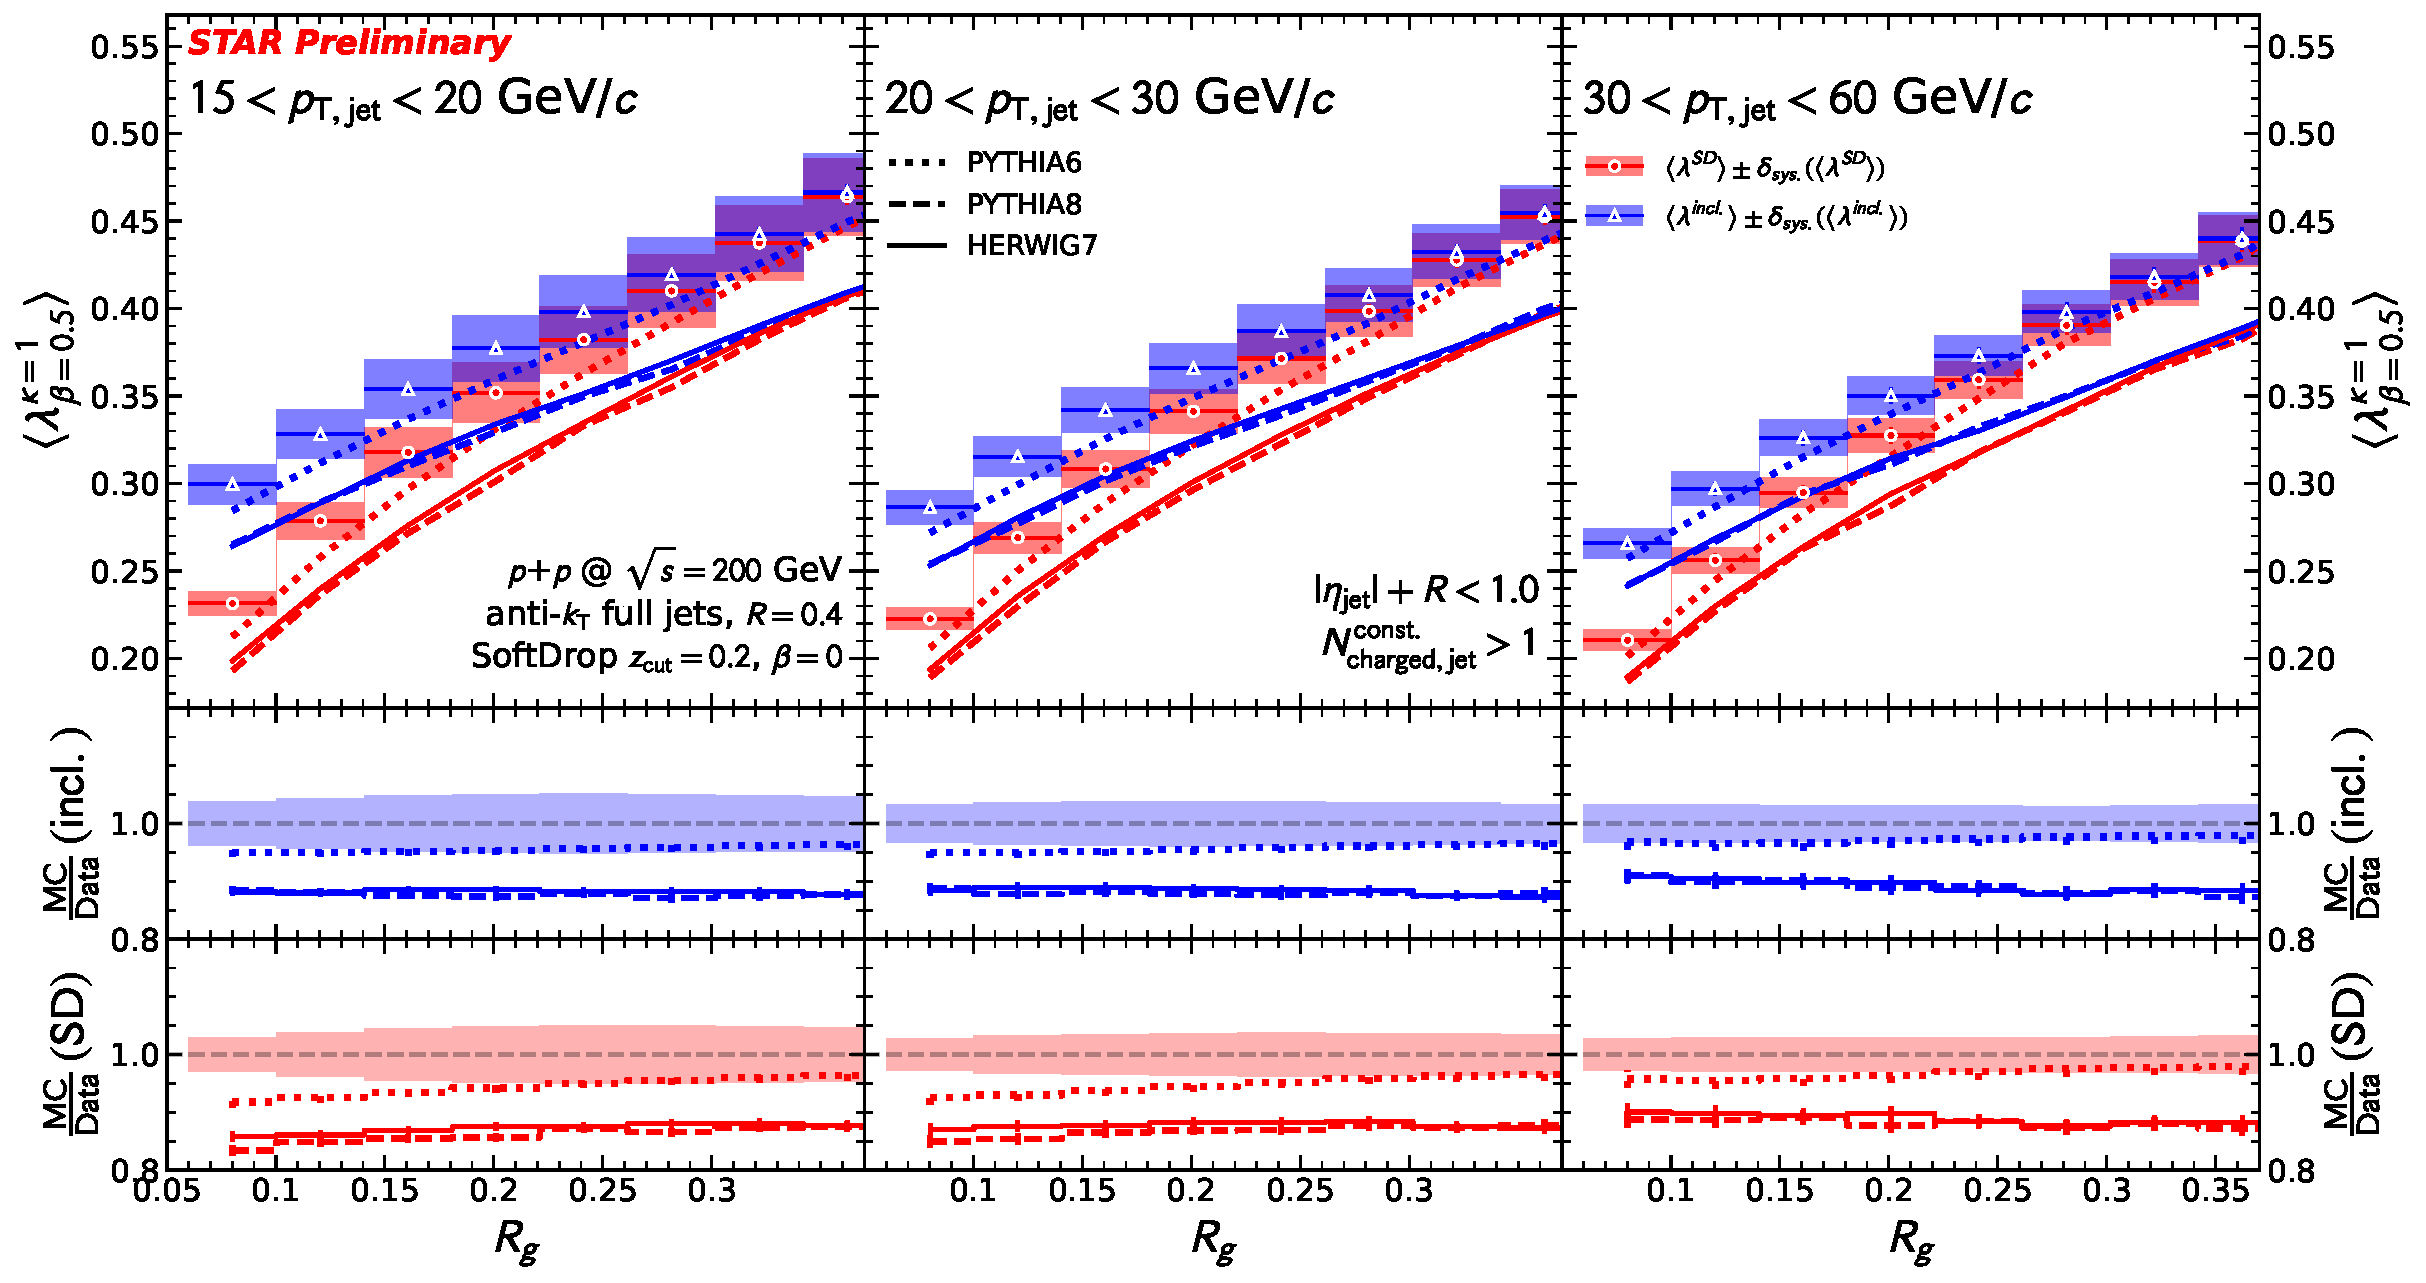
\includegraphics[width=0.9\linewidth]{angularities/pp/fig_prof_sd_dR_ptbins_ch_ang_k1_b0_5.pdf}
	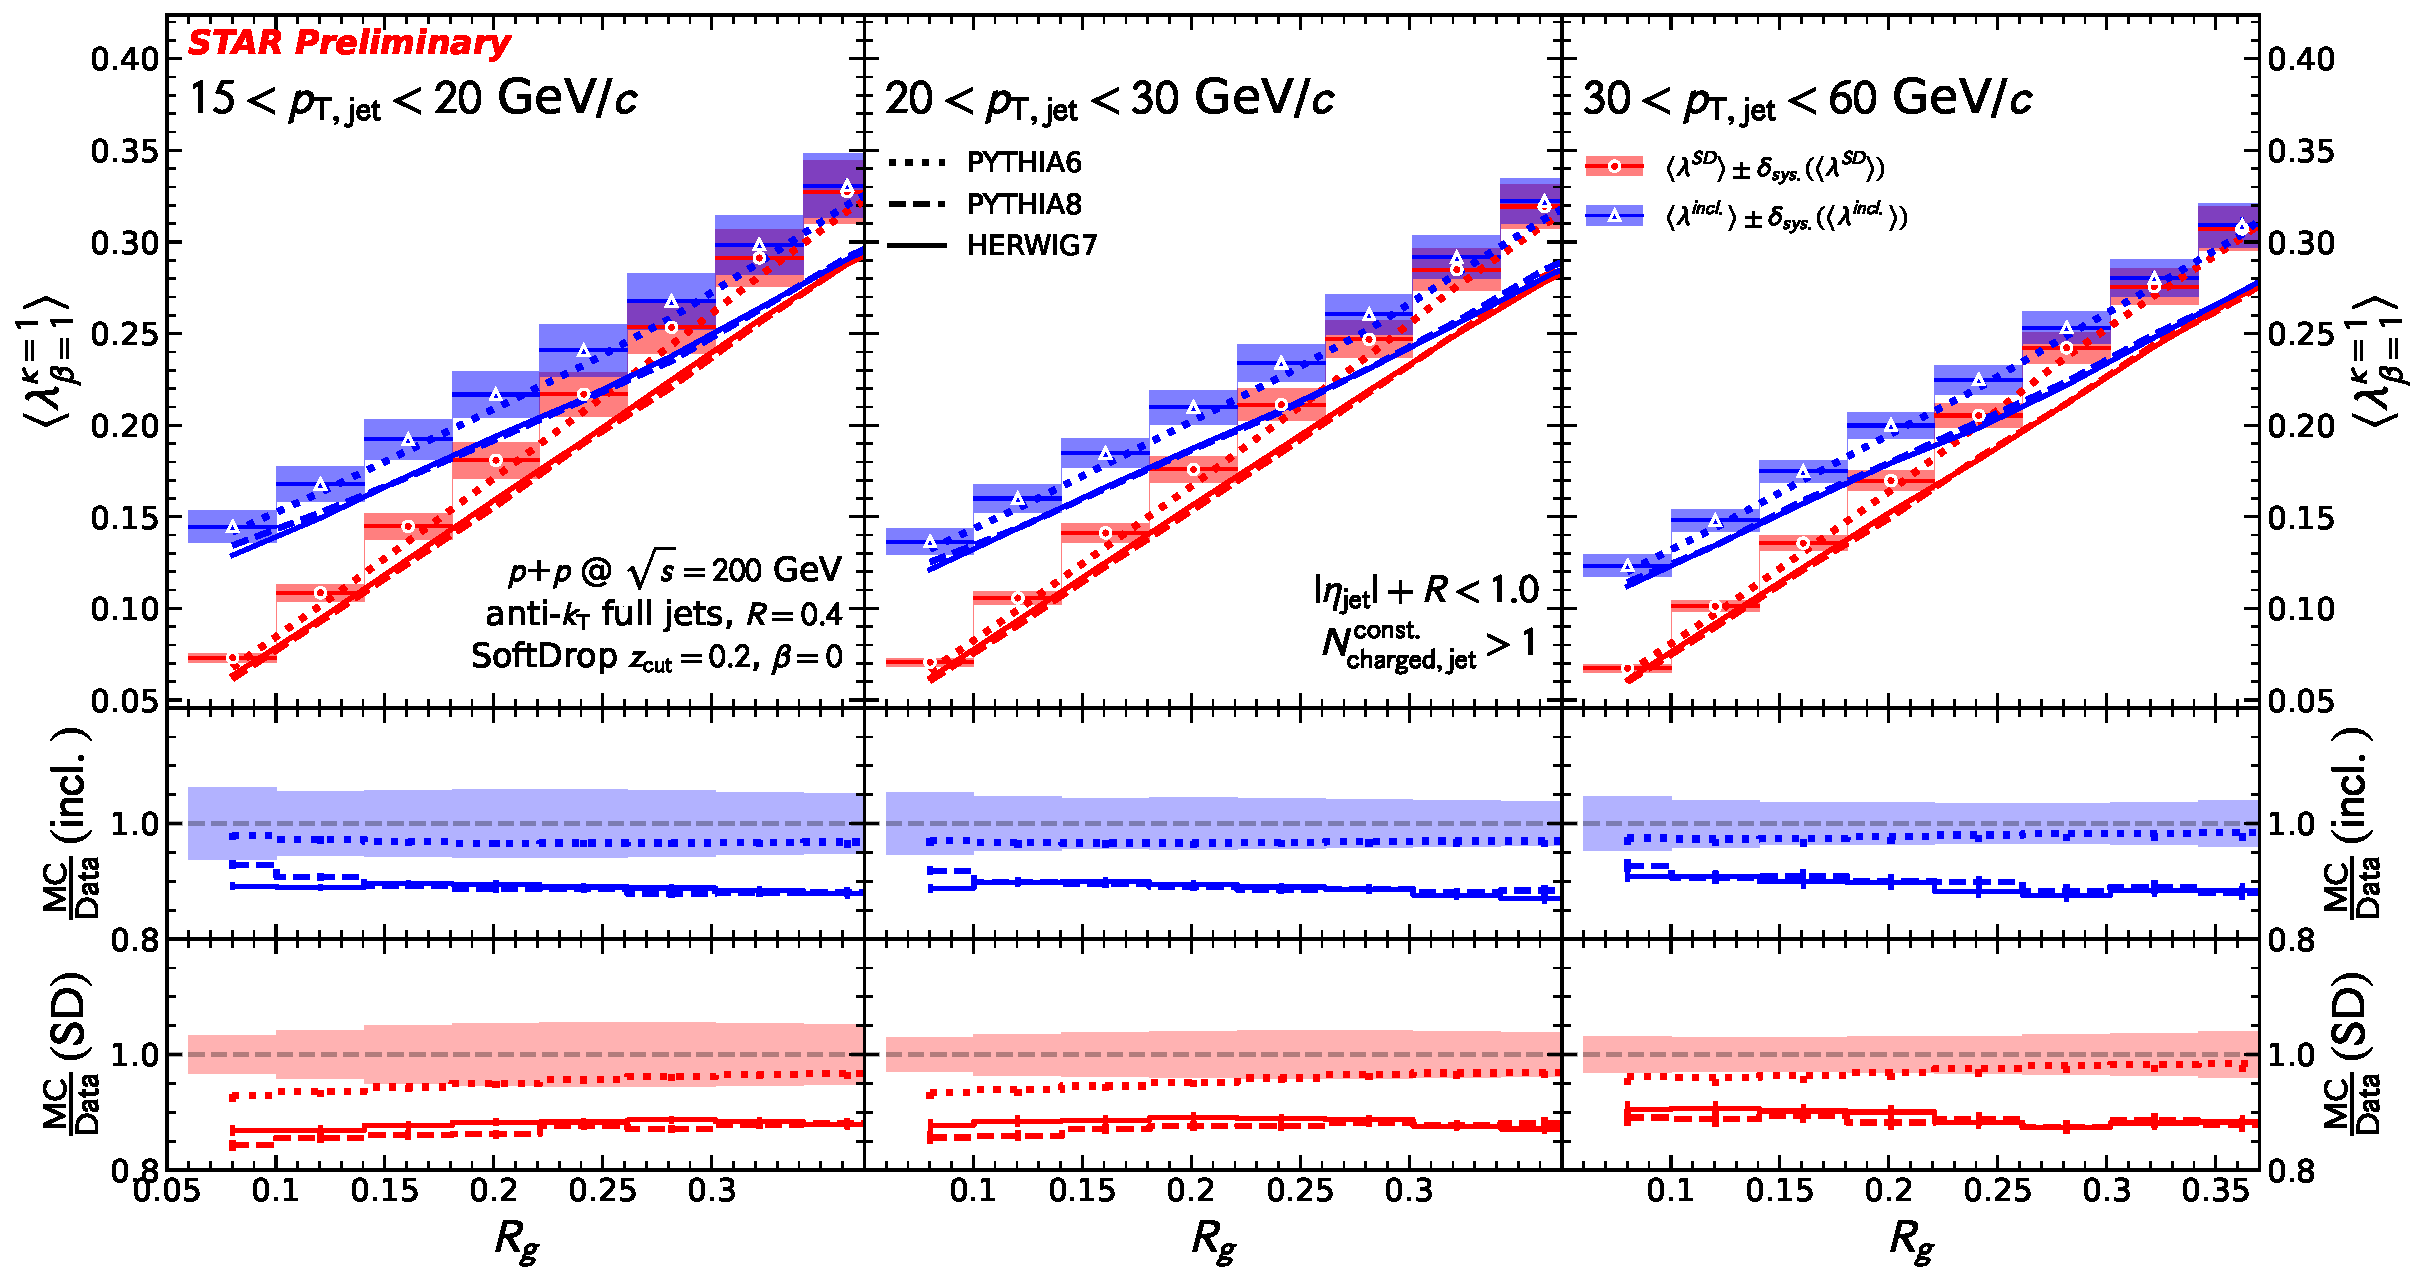
\includegraphics[width=0.9\linewidth]{angularities/pp/fig_prof_sd_dR_ptbins_ch_ang_k1_b1.pdf}
	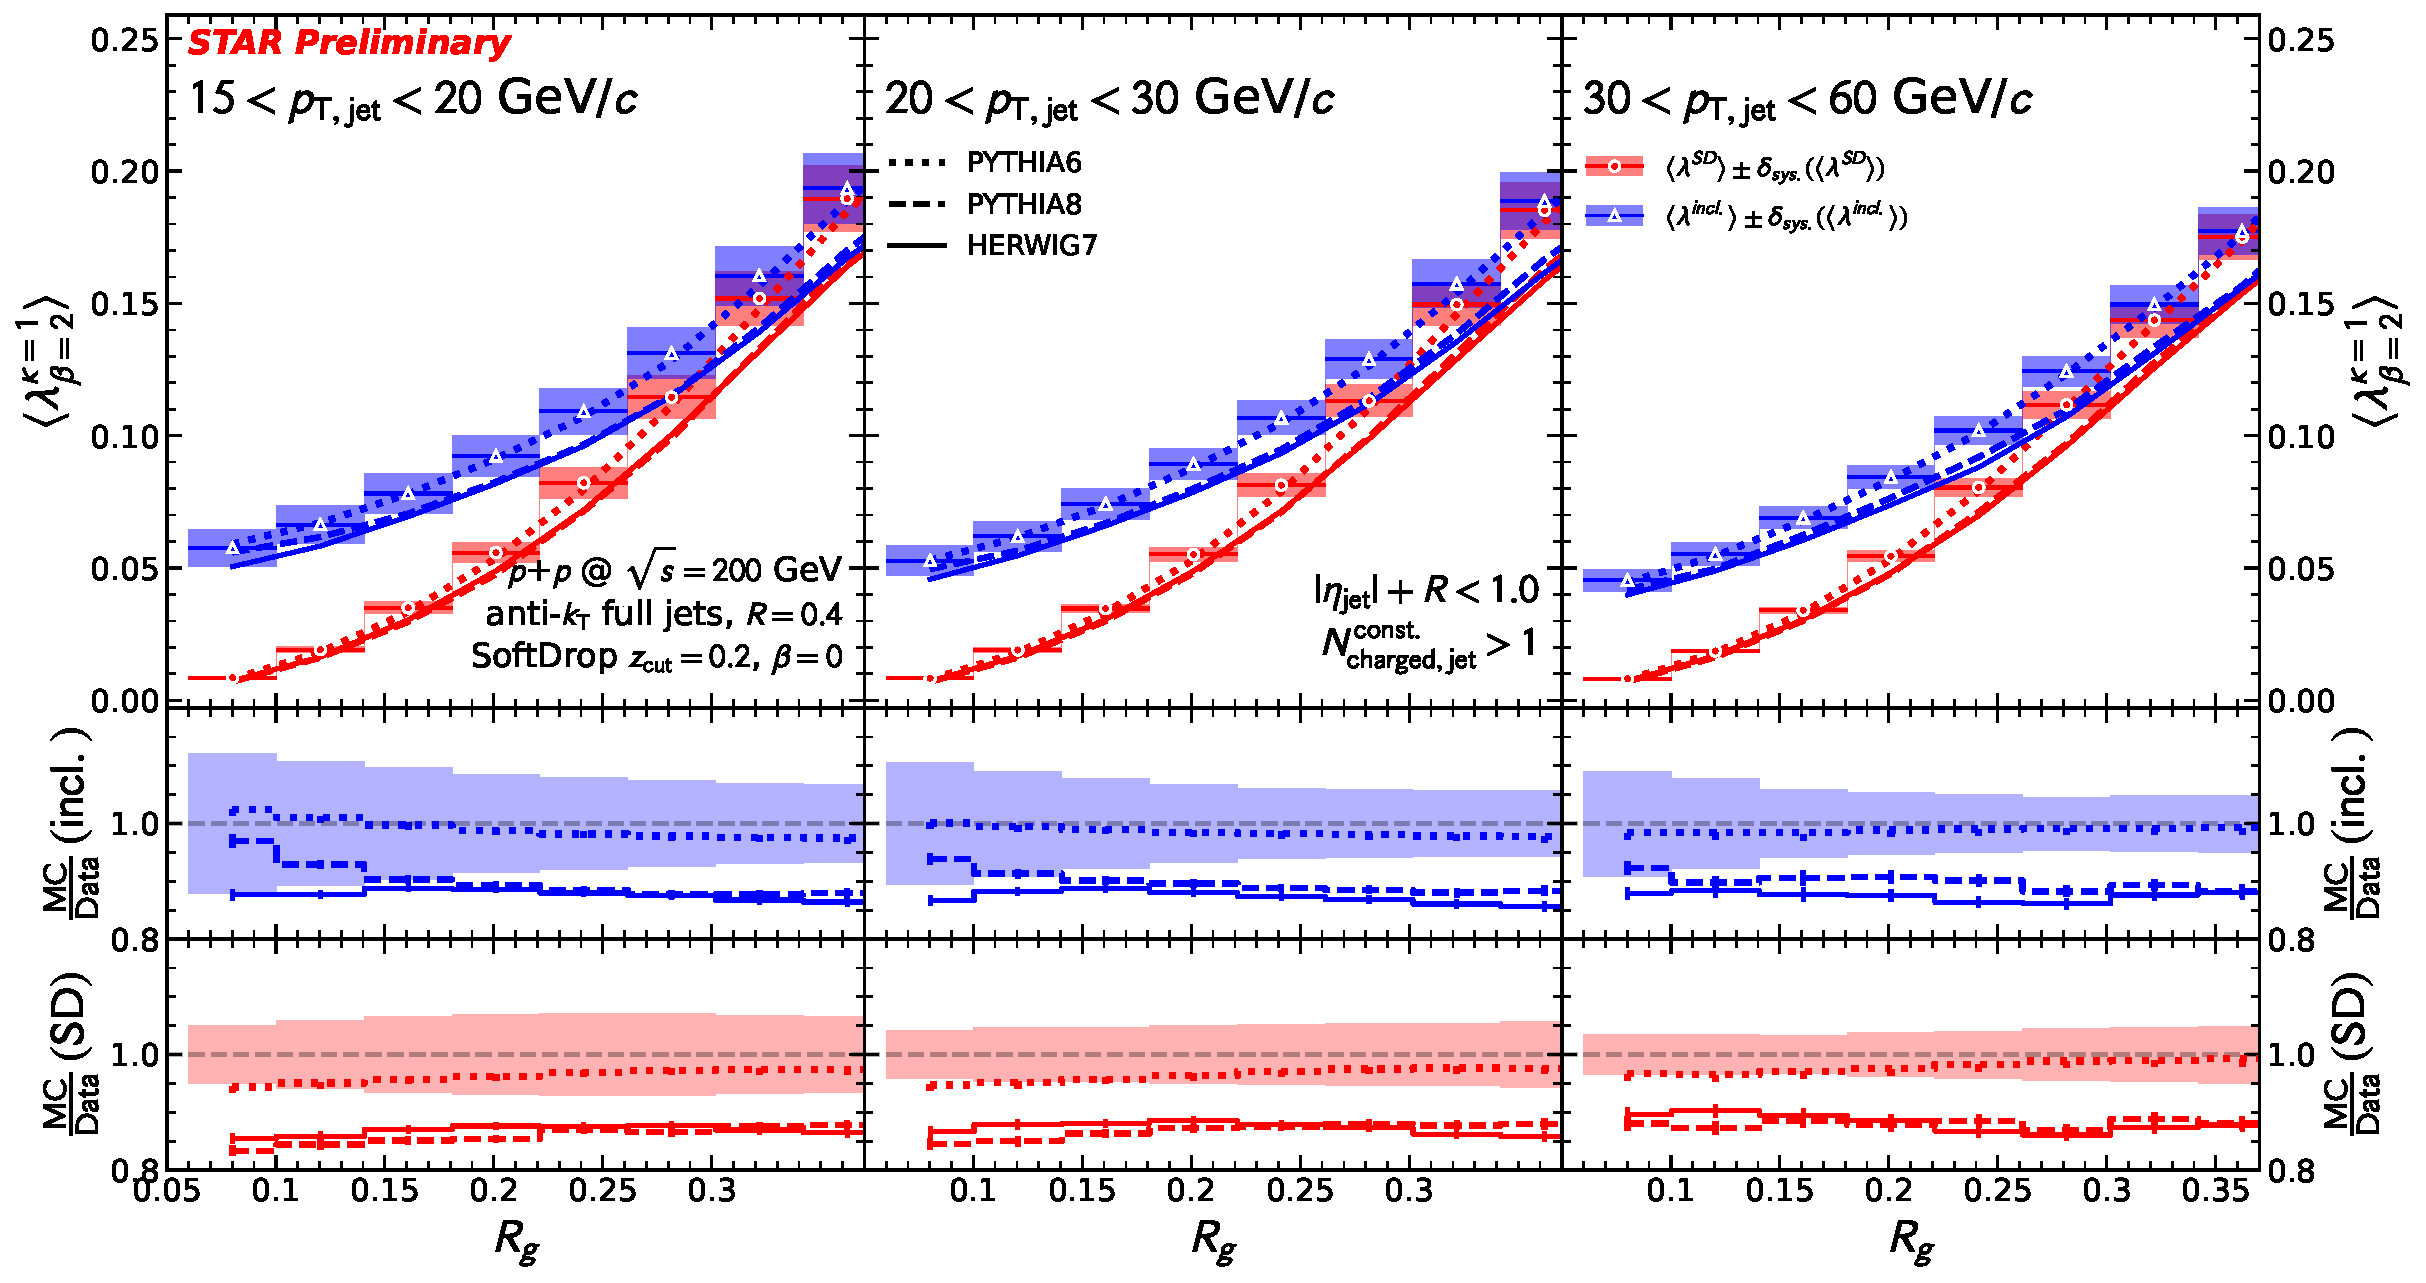
\includegraphics[width=0.9\linewidth]{angularities/pp/fig_prof_sd_dR_ptbins_ch_ang_k1_b2.pdf}
	\caption{Unfolded mean angularities \(\langle\lambda^{\kappa=1}_{\beta}\rangle\) as functions of the groomed radius \(R_\mathrm{g}\) for \(\beta = 0.5\), 1 and 2 (top to bottom) for inclusive (blue) and SoftDrop-groomed (red) jets in \(p+p\) collisions at \sPP{200}{GeV}, in three \(p_\mathrm{T, jet}\) ranges (columns). Boxes show the systematic and bars the statistical uncertainties. The measurements are compared to PYTHIA-6 (dotted), PYTHIA-8 (dashed) and HERWIG-7 (solid), and the lower panels show the ratios of the event generators to the data, with the relative systematic uncertainty of the data as a band.}
	\label{fig:ppProfRg}
\end{figure}

 \begin{figure}
	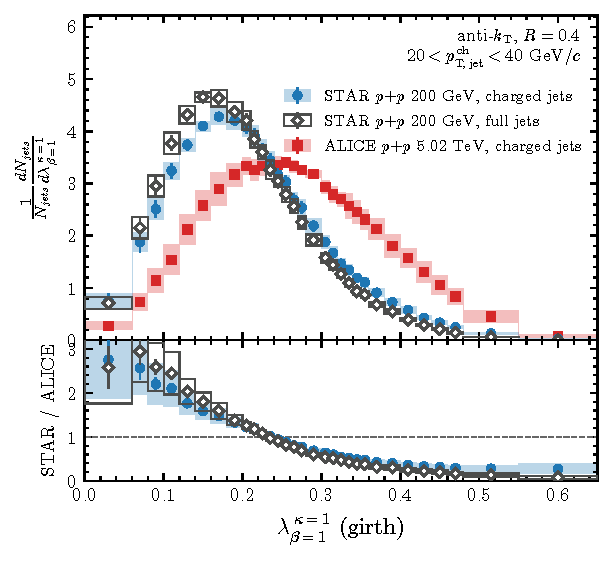
\includegraphics[width=0.49\linewidth]{angularities/pp/pub_comparison/alice_2107.11303/angularities_noptd/alice_ungroomed_lambda1_ptch20_40.pdf}
	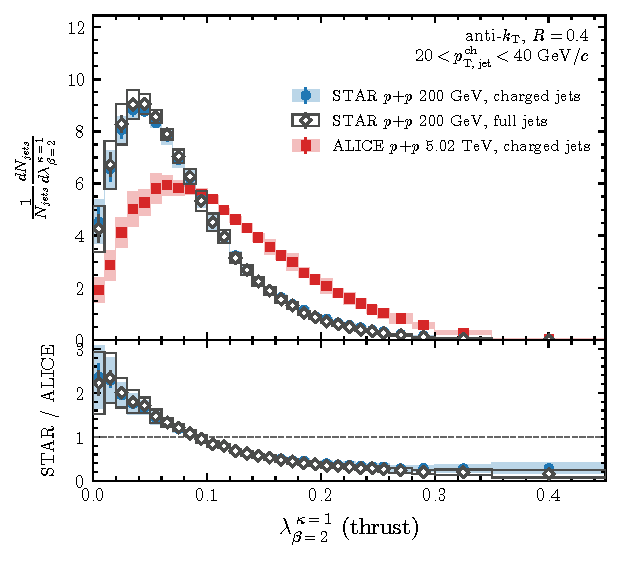
\includegraphics[width=0.49\linewidth]{angularities/pp/pub_comparison/alice_2107.11303/angularities_noptd/alice_ungroomed_lambda2_ptch20_40.pdf}
	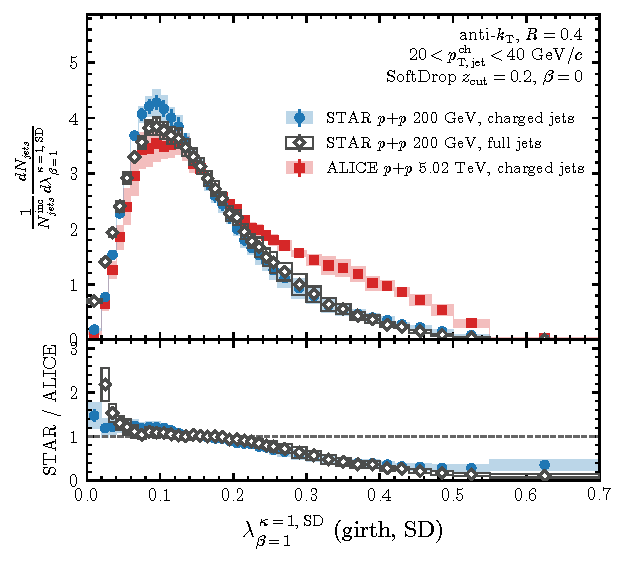
\includegraphics[width=0.49\linewidth]{angularities/pp/pub_comparison/alice_2107.11303/angularities_noptd/alice_groomed_lambda1_ptch20_40.pdf}
	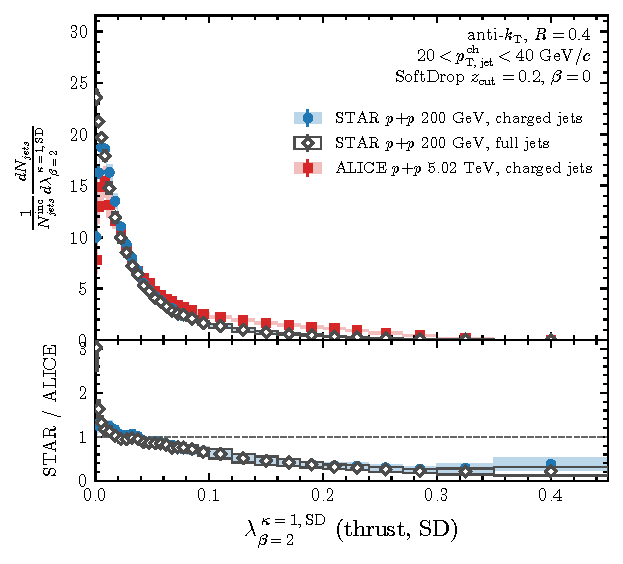
\includegraphics[width=0.49\linewidth]{angularities/pp/pub_comparison/alice_2107.11303/angularities_noptd/alice_groomed_lambda2_ptch20_40.pdf}
	\caption{Comparison with the ALICE measurement of \(p+p\) collisions at \(\sqrt{s} = 5.02\) TeV~\cite{ALICE:2021njq} (red) of ungroomed (top) and SoftDrop-groomed (bottom, \(z_\mathrm{cut} = 0.2\), \(\beta = 0\)) \(\lambda^{\kappa=1}_{\beta}\) distributions for \(\beta = 1\) (left) and 2 (right), for charged jets with \(20 < p_\mathrm{T, jet}^\mathrm{ch.} < 40\) GeV/\(c\). This work is shown for the charged-particle definition of ALICE (blue) and for the full jets of this analysis (black). The lower panels show the ratios to ALICE.}
	\label{fig:aliceComp}
\end{figure}
\section{Conclusion and Outlook}
\label{sec:angConclusion}
This chapter presented two measurements of jet angularities at \sNN{200}{GeV}, both corrected for detector effects with unbinned, machine-learning based unfolding.

The distributions of the girth \(g = \lambda_1^1\), \(p_\mathrm{T}^\mathrm{D} = \sqrt{\lambda_0^2}\) and LeSub of hard-core jets in Au+Au collisions (Sect.~\ref{sec:AuAuAngularities}, Fig.~\ref{fig:AuAu_JSO}) are consistent between central (0--20\%) and peripheral (40--80\%) collisions within the systematic uncertainties.
%
This absence of a visible modification is at least partly a consequence of the analysis choices: the hard-core constituent selection favors hard-fragmented, narrow jets, which interact less with the QGP, and the conservative, uncorrelated treatment of the systematic uncertainties in the central-to-peripheral ratio limits its sensitivity.
%
As the first heavy-ion measurement with unbinned unfolding, it also showed where the method needed to be developed further before being applied to less biased jets.

This development was carried out with the inclusive and SoftDrop-groomed angularities \(\lambda^{\kappa=1}_{\beta}\), \(\beta = 0.5\), 1 and 2, of inclusive jets in \(p+p\) collisions at \sPP{200}{GeV} (Sect.~\ref{sec:ppResults}).
%
The unfolding passes its closure tests and reproduces earlier STAR measurements of the jet mass, groomed jet mass, \(R_\mathrm{g}\) and \(z_\mathrm{g}\) from the same unfolded jets.
%
The measured jets become narrower with increasing \(p_\mathrm{T, jet}\), and grooming shifts the angularities to smaller values, the more so the larger \(\beta\).
%
PYTHIA-6, PYTHIA-8 and HERWIG-7 describe the main trends, but predict narrower jets than measured; PYTHIA-8 and HERWIG-7 fall 20--40\% below the data in the tails of the distributions, while PYTHIA-6 agrees within uncertainties in most bins.
%
For \(\beta = 1\) and 2, grooming reduces the deviations of PYTHIA-8 and HERWIG-7 from the data.
%
Because the unbinned unfolding keeps the full set of jet features, the mean angularities could also be measured as functions of the groomed radius \(R_\mathrm{g}\) without a dedicated analysis.
%
These profiles rise monotonically with \(R_\mathrm{g}\), with the groomed and inclusive values converging at large \(R_\mathrm{g}\) as expected from the angular ordering of the clustering sequence, and depend only weakly on \(p_\mathrm{T, jet}\) at fixed \(R_\mathrm{g}\).
%
They also show that PYTHIA-8 and HERWIG-7 underestimate the angularities by 10--15\% at every \(R_\mathrm{g}\), i.e.\ that their narrower jets come from too little radiation at a given splitting angle rather than from a different distribution of the splitting angle.
%
Compared with ALICE measurements at \(\sqrt{s} = 5.02\) TeV at the same charged-jet \(p_\mathrm{T}\), the jets at RHIC are considerably narrower, as expected from their larger fraction of quark-initiated jets.

These \(p+p\) results provide the baseline for the next step: measuring inclusive and groomed angularities of jets in Au+Au collisions at the same energy, with grooming in place of the hard-core selection to suppress the underlying event, and with the unfolding pipeline developed here.
%
Differential measurements such as the \(R_\mathrm{g}\) profiles are particularly promising there, since they can separate a medium-induced change of the radiation pattern at a given splitting angle from a change in the distribution of the splitting angles themselves.
%
In \(p+p\), the measurement will be extended by the angularities not shown here, such as \(\lambda_0^2\), for the final publication.


\chapter{Summary}
\label{ch:summary}
The jet-hadron correlations relative to the event plane of Ch.~\ref{ch:jhcorr} have been published by the STAR Collaboration in Phys.\ Rev.\ C~\textbf{109}, 044909 (2024)~\cite{STAR:2023hye}.
%
The generalized angularities of jets in \AuAu collisions (Sec.~\ref{sec:AuAuAngularities}) were shown as STAR preliminary results at the 30\(^\text{th}\) International Conference on Ultra-relativistic Nucleus-Nucleus Collisions (Quark Matter 2023)~\cite{Pani:2024mgy}.
%
Earlier iterations of the \pp angularities of Sec.~\ref{sec:ppResults} were presented orally at the 11\(^\text{th}\) International Conference on Hard and Electromagnetic Probes of High-Energy Nuclear Collisions (Hard Probes 2023)~\cite{Pani_2024} and as posters at Hard Probes 2024 and Hard Probes 2026, and some of the recommendations of this work for unbinned unfolding are featured in a community white paper~\cite{Canelli_2026}.

This thesis uses jets, the collimated sprays of hadrons that trace the quarks and gluons of a hard scattering, to study QCD in vacuum and in the quark-gluon plasma at RHIC.
%
Ch.~\ref{ch:intro} built the necessary picture: the color charge and the non-Abelian \(\mathrm{SU}(3)\) symmetry of QCD, the running of \(\alpha_s\) that separates the perturbative hard scattering and parton shower from the non-perturbative hadronization, and the event generators that model these stages.
%
Because soft gluon radiation is ordered in angle (App.~\ref{app:theory}), the angular distribution of energy inside a jet records the history of its shower, which is what the angularities of Ch.~\ref{ch:angularities} measure.
%
All measurements use the STAR TPC for charged tracks and the BEMC for neutral energy and triggering (Ch.~\ref{ch:STAR}), and rest on the event-plane reconstruction (App.~\ref{sec:EP_Recon}), the machine-learning tools (App.~\ref{app:ML}) and the unfolding framework (App.~\ref{app:Unfolding}) described in the appendices, in which binned Iterative Bayesian Unfolding and unbinned MultiFold are the same algorithm, differing only in how the reweighting ratios are estimated.

\paragraph{Path-length dependence of jet quenching.}
Ch.~\ref{ch:jhcorr} measured the distributions of charged hadrons relative to jets with \pttrigrange{15}{20} and \pttrigrange{20}{40} in 20--50\% central \AuAu collisions at \sNN{200}{GeV}, separately for jets in-, mid- and out-of-plane with respect to the second-order event plane, as the angle to the event plane is correlated with the average path length through the medium.
%
The large, flow-modulated combinatorial background was removed with the reaction plane fit, which constrains the background by fitting all three orientations simultaneously at large \deta, while the pair acceptance was corrected with mixed events and the orientation-dependent underlying-event contribution to the jet momentum with random cones.
%
Within the uncertainties, neither the associated yields nor the widths of the jet peaks show a dependence on the event plane.
%
The ratios of the associated yields between the orientations do not deviate significantly from unity, with indications of potential modifications only in the inclusive \ptassocrange{1.0}{10} bin of the \pttrigrange{20}{40} jets.
%
Any real dependence is diluted by the finite event-plane resolution, \(R_2 = 0.56\): a constituent anisotropy of \(v_2 = 0.1\) would reduce the out-of-plane to in-plane ratio only to 0.81 instead of 0.67.
%
JEWEL predicts an event-plane dependence well below the uncertainties, consistent with jet-by-jet fluctuations dominating over path-length effects, and describes the data better with recoils at low \Pt{assoc} and without them at high \Pt{assoc}.

\paragraph{Jet substructure in \AuAu collisions.}
Sec.~\ref{sec:AuAuAngularities} presented the girth \(g = \lambda_1^1\), \(p_\mathrm{T}^\mathrm{D} = \sqrt{\lambda_0^2}\) and LeSub of hard-core jets in 0--20\% and 40--80\% central \AuAu collisions, the first heavy-ion measurement corrected with unbinned, machine-learning based unfolding.
%
The distributions are consistent between central and peripheral collisions within the systematic uncertainties.

\paragraph{Inclusive and groomed angularities in \pp collisions.}
Sec.~\ref{sec:ppResults} presented the inclusive and SoftDrop-groomed angularities \(\lambda^{\kappa=1}_{\beta}\), \(\beta = 0.5\), 1 and 2, of inclusive jets in \pp collisions at \sPP{200}{GeV}, unfolded with MultiFold using 23 features per jet.
%
The unfolding passes its closure tests and, from the same unfolded jets, reproduces the jet mass, groomed jet mass, \(R_\mathrm{g}\) and \(z_\mathrm{g}\) previously published by STAR.
%
The jets become narrower with increasing \(p_\mathrm{T, jet}\), and grooming shifts the angularities to smaller values, the more so the larger \(\beta\).
%
PYTHIA-6, PYTHIA-8 and HERWIG-7 reproduce these trends but predict jets that are narrower than measured: PYTHIA-8 and HERWIG-7 fall 20--40\% below the data in the tails of the distributions, while PYTHIA-6 agrees within uncertainties in most bins, and for \(\beta = 1\) and 2 grooming reduces the deviations of PYTHIA-8 and HERWIG-7.

Because the unbinned unfolding keeps the full set of jet features, the mean angularities could also be measured as functions of the groomed radius \(R_\mathrm{g}\), an observable that was not chosen before the unfolding.
%
The profiles rise monotonically with \(R_\mathrm{g}\), the groomed and inclusive values converge at large \(R_\mathrm{g}\), as expected from the angular ordering of the clustering sequence, and at fixed \(R_\mathrm{g}\) they depend only weakly on \(p_\mathrm{T, jet}\).
%
PYTHIA-8 and HERWIG-7 underestimate them by 10--15\% at every \(R_\mathrm{g}\), which shows that their narrower jets come from too little radiation at a given splitting angle rather than from a different distribution of splitting angles.
%
Compared with ALICE at \(\sqrt{s} = 5.02\)~TeV at the same charged-jet \(p_\mathrm{T}\), the jets at RHIC are considerably narrower, as expected from their larger fraction of quark-initiated jets.

\paragraph{Synthesis.}
Both heavy-ion measurements select jets with a high-tower trigger and hard-core constituents, a selection that favors hard-fragmented, narrow jets that interact least with the medium.
%
This survivor bias is the likely common reason why neither the expected path-length dependence nor a centrality dependence of the substructure is observed.
%
The \pp measurement avoids this selection and provides both the baseline and a validated unbinned unfolding pipeline for the next generation of heavy-ion measurements.

\section{Outlook}
The natural next step is to measure the inclusive and groomed angularities of jets in \AuAu collisions with the inclusive constituent selection and SoftDrop grooming of the \pp analysis, unfolded with the same pipeline, so that the \pp results can serve as the baseline they were designed to be.
%
There, the \(R_\mathrm{g}\) profiles can separate a medium-induced change of the radiation at a given splitting angle from a change of the distribution of the splitting angles themselves, a distinction that one-dimensional distributions cannot make.
%
The larger background of heavy-ion collisions makes missed and fake jets far from negligible, which the unfolding framework of App.~\ref{app:Unfolding} already treats explicitly.

The unfolding itself can be made more robust.
%
Recent methods that replace the particle-level step of OmniFold by a single loss function remove the need for iterations and reduce the dependence on the reference simulation~\cite{Ore:2026qgp}, which would avoid the growth of statistical fluctuations over the iterations seen in this work, and profiling the uncertainties of the detector simulation as nuisance parameters during the unfolding~\cite{Zhu:2024drd} would give a more principled treatment of the systematic uncertainties than the separate variations used here.
%
Richer jet representations, such as images of the constituents, could let the classifiers use more of the information in a jet.

On the jet-hadron side, selecting events on the ellipticity of their initial state through the \(q_n\) flow vector within a centrality class would test whether fluctuations of the initial geometry wash out the event-plane dependence.
%
The quark-gluon and quenched-unquenched classifiers of App.~\ref{app:ML} suggest that the amount of medium modification can itself be quantified as a discrimination problem, which extends naturally to the angularities once groomed heavy-ion measurements are available.
%
Finally, the \pp measurement will be extended with \(\lambda_0^2\) and the remaining angularities for the final STAR publication.


% R E F E R E N C E S
\def\aap{{A\&A}}
\def\aas{{A\&AS}}
\def\aj{{AJ}}
\def\araa{{ARA\&A}}
\def\apj{{ApJ}}
\def\apjl{{ApJ}}
\def\apjs{{ApJS}}
\def\baas{{BAAS}}
\def\mnras{{MNRAS}}
\def\nat{{Nature}}
\def\pasp{{PASP}}

\clearpage
\addcontentsline{toc}{chapter}{Bibliography}
\bibliographystyle{unsrt}
\begingroup
\setlength{\bibsep}{11pt}
\linespread{1}\selectfont
\bibliography{thesis}
\endgroup

% A P P E N D I X
\appendix

\chapter{Hard Processes and Parton Showers}
\label{app:theory}
\section{The QCD Lagrangian}
\label{sec:qcdLagrangian}
The color symmetry of Sec.~\ref{sec:QCDIntro} is made precise by the QCD Lagrangian,
\begin{align}
	\mathcal{L}_\mathrm{QCD} = &\underbrace{\bar{q}^\alpha (i \gamma^\mu \partial_\mu\delta_{\alpha\beta} - g\gamma^\mu
		t^a_{\alpha\beta}A^a_\mu - m\delta_{\alpha\beta})q^\beta - \frac{1}{4} F^a_{\mu\nu}F_a^{\mu\nu}}_{\mathcal{L}_\mathrm{classical}}\notag\\ &\underbrace{- \frac{1}{2\lambda}(\partial^\mu A^a_\mu)^2}_{\mathcal{L}_\mathrm{gauge-fixing}}+ \underbrace{\bar{c}^\alpha\partial^\mu(\partial_\mu\delta_{\alpha\beta} + igT^a_{\alpha\beta}A^a_\mu)c^\beta}_{\mathcal{L}_\mathrm{ghost}}
\end{align}

\(\mathcal{L}_\mathrm{classical}\) is the classical Lagrangian density shows interaction of a quark field  \(q^\alpha\) with 3 color degrees of freedom interacting with gluon fields \(A^a_\mu\) with 8 color degrees of freedom. \(g\) and \(m\) are dimensionless and correspond to QCD coupling constant, and quark-mass respectively. \(F^a_{\mu\nu}\) are the gluon tensors defined as,
\begin{equation}
	F^a_{\mu\nu} = \partial_\mu A_\nu^a - \partial_\nu A_\mu^a - gf_{abc}A^b_\mu A^c_\nu.
	\label{eq:gluonFieldTensor}
\end{equation}

To properly define gluon propagators, we need to make a choice of gauge. The \(\mathcal{L}_\mathrm{gauge-fixing}\) parametrizes the class of covariant gauges with the gauge parameter $\lambda$. In non-Abelian theories, this gauge fixing term leads to creation of unphysical degrees of freedom, which are canceled out by \(\mathcal{L}_\mathrm{ghost}\) which contains complex, scalar fermion fields \(c^\alpha\). 

The matrices \(t^a\) and  \(T^a\) are the fundamental and adjoint representations of \(\rm SU(3)\) in form of traceless \(3\times3\) and \(8\times8\) hermitian matrices satisfying:
\begin{align}
	[t^a, t^b] = if_{abc}t^c,~\tr(t^at^b) = \frac{1}{2}\delta^{ab} \notag\\
	[T^a, T^b] = if_{abc}T^c,~(T^{a})_{bc} = -if^{abc}.
\end{align}

Comparing with quantum electrodynamics (QED), where the photon field tensor lacks the last term of Eq.~\ref{eq:gluonFieldTensor} as it is an Abelian, \(U(1)\) gauge theory, we can explain the presence of three/four-gluon vertices and absence of such vertices for the photon in Fig.~\ref{fig:smvtx}. The Lagrangian can be used to formulate \emph{Feynman rules} for calculating amplitude contributions from various propagators and vertices, which are collected in Tab.~\ref{tab:qcdrules}.

\begin{table}[htbp]
	\centering
	\begin{tabular}{
		>{\centering\arraybackslash}m{4.0cm}
		>{\raggedright\arraybackslash}m{10.4cm}
		}
		% --- PROPAGATORS
		\propagator{gluon}{A,\alpha}{B,\beta}{p}                                       &
		\(\delta^{AB}\left[-g^{\alpha\beta} + (1-\lambda)\dfrac{p^{\alpha}p^{\beta}}{p^{2}+i\epsilon}\right]
		\dfrac{i}{p^{2}+i\epsilon}\)                                                                                                                                                       \\[0.4cm]

		\propagator{ghost}{A}{B}{p}                                                    &
		\(\delta^{AB}\,\dfrac{i}{p^{2}+i\epsilon}\)                                                                                                                                        \\[0.4cm]

		\propagator{fermion}{a,i}{b,j}{p}                                              &
		\(\delta^{ab}\,\dfrac{i}{(\slashed{p}-m+i\epsilon)_{ji}}\)                                                                                                                         \\[0.6cm]

		% --- VERTICES
		\yvertex{gluon}{B,\beta}{q}{gluon}{A,\alpha}{p}{gluon}{C,\gamma}{r}            &
		\(-g\,f^{ABC}\left[(p-q)^{\gamma}g^{\alpha\beta} + (q-r)^{\alpha}g^{\beta\gamma}
			+ (r-p)^{\beta}g^{\gamma\alpha}\right]\)

		\smallskip

		(all momenta incoming, \(p+q+r=0\))                                                                                                                                                \\[0.4cm]

		\fourvertex{gluon}{A,\alpha}{gluon}{C,\gamma}{gluon}{B,\beta}{gluon}{D,\delta} &
		\(\begin{aligned}
			  -ig^{2}f^{XAC}f^{XBD}\left[g^{\alpha\beta}g^{\gamma\delta} - g^{\alpha\delta}g^{\beta\gamma}\right] \\
			  -ig^{2}f^{XAD}f^{XBC}\left[g^{\alpha\beta}g^{\gamma\delta} - g^{\alpha\gamma}g^{\beta\delta}\right] \\
			  -ig^{2}f^{XAB}f^{XCD}\left[g^{\alpha\gamma}g^{\beta\delta} - g^{\alpha\delta}g^{\beta\gamma}\right]
		  \end{aligned}\) \\[0.4cm]

		\yvertex{gluon}{A,\alpha}{}{ghost}{B}{}{ghost}{C}{q}                           &
		\(g\,f^{ABC}q^{\alpha}\)                                                                                                                                                           \\[0.4cm]

		\yvertex{gluon}{A,\alpha}{}{fermion}{b,i}{}{fermion}{c,j}{}                    &
		\(-ig\,(t^{A})_{cb}\,(\gamma^{\alpha})_{ji}\)
	\end{tabular}
	\caption{Feynman rules for QCD in a covariant gauge with gauge parameter \(\lambda\):
		the gluon, ghost and quark propagators, followed by the three- and four-gluon,
		ghost-gluon and quark-gluon vertices.}
	\label{tab:qcdrules}
\end{table}
\section{Hard Processes}
\label{sec:hardProcesses}
To consider any nucleus as a singular coherent object, the fluctuations inside it would involve momentum transfers below the confinement scale (\(\Lambda\)) introduced in Sec.~\ref{subsec:runningCoupling}, and would occur over timescales \(\sim 1/\Lambda\). We define \emph{hard-scattering processes} or just \emph{hard processes} as interactions of a hard perturbative probe with high momentum transfer \(Q >> \Lambda\). Since this interaction occurs over a time-scale \(\sim 1/Q \ll 1/\Lambda\), the perturbative probe effectively interacts with a near-static ``snapshot'' of the nucleus with a characteristic resolution \(\sim 1/Q\).

\begin{figure}[htbp]
	\centering
	\factorizationdiagram
	\caption{Collinear factorization of a hadronic hard scattering.}
	\label{fig:factorization}
\end{figure}

Thus, the cross sections of a collision process of nuclei with momentum \(P_1\) and \(P_2\) depicted by Fig.~\ref{fig:factorization} can be \emph{factorized} into various independent components as,

\begin{equation}
	\frac{d\sigma}{d\mathbf{O}}  = \sum_{i,j,f} \int dx_1dx_2d\mathbf{\Phi}_ff_i(x_1, \mu^2)f_j(x_2, \mu^2)\frac{d\hat{\sigma}_{ij\to f}}{d\hat{\mathbf{O}}}D_f(\hat{\mathbf{O}}\to\mathbf{O}, \mu^2)
	\label{eq:factorization}
\end{equation}

Where, the interactions occur between partons \(i\) from nucleus 1 and \(j\) from nucleus 2 carrying momentum \(p_1 = x_1P_1\) and \(p_2 = x_2P_2\) respectively. \(\mu\) is an arbitrary \emph{factorization scale}, often just set to \(Q\). The \(f_{k}(x, \mu^2)\) are the \emph{parton densities} giving likelihood of a parton \(k\) to carry \(x\) fraction of its parent nucleus's momentum at a particular factorization scale \(\mu\). \(f\) labels the partonic final state coming out of the scattering and \(\mathbf{\Phi}_f\) is its phase space. \(\hat{\sigma}_{ij\to f}\)  is the \emph{parton cross-section} for scattering of partons \(i\) and \(j\) into \(f\), kept differential in a partonic observable \(\hat{\mathbf{O}}\). We can approximate it to the \((n+k)\) order in \(\alpha_s\) as,

\begin{equation}
	\frac{d\hat{\sigma}_{ij\to f}}{d\hat{\mathbf{O}}} = \alpha_s^k \sum_{m=0}^{n}\alpha_s^m\,\frac{d\hat{\sigma}^{(m)}_{ij\to f}}{d\hat{\mathbf{O}}}(p_1, p_2, Q^2/\mu^2)
	\label{eq:partonXsecOrders}
\end{equation}

Different hard processes will have different leading powers \(k\). \(W\) production will have \(k=0\) whereas perturbative dijet production with two outgoing quarks will have \(k=2\).

The \(D_f(\hat{\mathbf{O}}\to\mathbf{O}, \mu^2)\) are the \emph{fragmentation functions}, giving the likelihood of a partonic final state with \(\hat{\mathbf{O}}\) being measured as \(\mathbf{O}\) once hadronization is over.
%
Like the parton densities, they cannot be calculated in perturbation theory, but they are \emph{universal}: once measured in one process they can be used in any other, and their dependence on \(\mu\) is governed by evolution equations of the same kind as the running of \(\alpha_s\) (Sec.~\ref{subsec:runningCoupling}).
%
Eq.~\ref{eq:factorization} is the skeleton of every measurement presented in this thesis, with the choice of \(\mathbf{O}\) being what separates one from the next, and a measurement is comparable to a calculation only if both use the same \(\mathbf{O}\).
%
Restricting \(\mathbf{O}\) to charged particles, as will be done for the angularities of Ch.~\ref{ch:angularities}, puts that restriction into \(D_f\) as well, and the non-perturbative input can then no longer be avoided.
%
The nuclear modification factors of Sec.~\ref{sec:jetsInQGP} are ratios of Eq.~\ref{eq:factorization} between two collision systems, where the parton densities largely cancel and what is left is the effect of the medium on \(\hat{\sigma}_{ij\to f}\) and \(D_f\).

%The parton densities \(f_i(x,\mu^2)\) in Eq.~\ref{eq:factorization} are not calculable in perturbation theory, but they are \emph{universal}: once measured in one process they may be used to predict any other. Requiring the physical cross section of Eq.~\ref{eq:factorization} to be independent of the arbitrary scale \(\mu\), exactly as for the coupling in Sec.~\ref{subsec:runningCoupling},
%\begin{equation}
%	\mu^2\frac{d}{d\mu^2}\,\sigma(P_1,P_2) = 0,
%	\label{eq:pdfRGE}
%\end{equation}
%ties the \(\mu\)-dependence of the densities to that of \(\hat{\sigma}_{ij}\).

%\section{Dijet events}
%Where, \(\overline{\sum}\)  denotes  the average and sum over the spins and colors of initial and final partons \(\{i, j, k, l\}\) and \(\hat{s} = (p_1+p_2)^2\). To get the dijet cross-section, we insert the parton cross-section from Eq.~\ref{eq:partonxsec} into  Eq.~\ref{eq:factorization}. Assuming the incoming partons are massless and collinear with the beams, \(p_1 = \frac{1}{2}x_1\sqrt{s}(1, 0, 0, 1)\) and \(p_2 = \frac{1}{2}x_2\sqrt{s}(1, 0, 0, -1)\), so that \(\hat{s} = x_1x_2s\),
%
%\begin{align*}
%	\frac{E_3E_4d^6\sigma}{d^3p_3d^3p_4} & = \frac{1}{2s}\frac{1}{16\pi^2} \sum_{\{i,j,k,l\}\subset q\bigcup\bar{q}\bigcup g} \frac{1}{1 + \delta_{kl}} \int dx_1dx_2 \frac{f_i(x_1, \mu^2)}{x_1} \frac{f_j(x_2, \mu^2)}{x_2} \\
%	& \qquad \times\, \overline{\sum}|\mathcal{M}(ij\rightarrow kl)|^2\delta^4(p_1 + p_2 - p_3 - p_4) 
%\end{align*}
%Where \(q\bigcup\bar{q}\bigcup g\) represents all the partonic states \(\{g, u, \bar{u}, d, \ldots\}\). 
%
%%	The four-momentum conserving \(\delta\)-function factorizes into a transverse part and the energy and longitudinal parts, 
%%	
%%	\begin{align*}
%		%	\delta^4(p_1 + p_2 - p_3 - p_4)                                & = \delta^2(\mathbf{p}_{T3} + \mathbf{p}_{T4})\,\delta\left(\tfrac{1}{2}\sqrt{s}(x_1 + x_2) - E_3 - E_4\right)                 \\
%		%	                                                               & \qquad \times\, \delta\left(\tfrac{1}{2}\sqrt{s}(x_1 - x_2) - p_{z3} - p_{z4}\right) \\
%		%	                                                               & = \frac{2}{s}\delta^2(\mathbf{p}_{T3} + \mathbf{p}_{T4})\,\delta\left(x_1 - \tfrac{1}{2}x_T(e^{y_3} + e^{y_4})\right)         \\
%		%	                                                               & \qquad \times\, \delta\left(x_2 - \tfrac{1}{2}x_T(e^{-y_3} + e^{-y_4})\right)
%		%\end{align*}
%		%
%		%Where, \(x_T \equiv 2p_T/\sqrt{s}\) and \(p_T \equiv p_{T, 3} = p_{T, 4}\),
%		%
%		%\begin{equation}
%		%	\frac{d^3\sigma}{dy_3dy_4dp_T^2} = \frac{1}{16\pi s^2}\sum_{\{i,j,k,l\}\subset q\bigcup\bar{q}\bigcup g} \frac{1}{1 + \delta_{kl}} \frac{f_i(x_1, \mu^2)}{x_1}\frac{f_j(x_2, \mu^2)}{x_2} \overline{\sum}|\mathcal{M}(ij\rightarrow kl)|^2
%		%\end{equation}
%		
%		Integrating Eq.~\ref{eq:partonxsec} over one of the outgoing partons gives the
%		\emph{single-inclusive} parton cross-section for the other.  Writing
%		\(q \equiv p_1 + p_2 - p_3\),
%		\begin{align}
%				\frac{E_3d^3\hat{\sigma}}{d^3p_3} &= \frac{1}{2\hat{s}}\frac{1}{16\pi^2}\overline{\sum}|\mathcal{M}|^2\int\frac{d^3p_4}{E_4}\,\delta^4(p_1 + p_2 - p_3 - p_4)                              \notag                      \\
%				&=\frac{1}{2\hat{s}}\frac{1}{16\pi^2}\overline{\sum}|\mathcal{M}|^2\int\frac{d^3p_4}{E_4}\,\delta^3(\mathbf{q} - \mathbf{p}_4)\,\delta(q^0 - E_4) \notag \\
%				&= \frac{1}{2\hat{s}}\frac{1}{16\pi^2}\overline{\sum}|\mathcal{M}|^2\,\frac{\delta(q^0 - |\mathbf{q}|)}{|\mathbf{q}|}       \notag \\  
%				&= \frac{1}{2\hat{s}}\frac{1}{16\pi^2}\overline{\sum}|\mathcal{M}|^2\,2\delta(q^2)                  
%			\end{align}
%		We can represent \(q^2\) in terms of partonic Mandelstam variables \(\hat{s} = (p_1+p_2)^2\), \(\hat{t} = (p_1-p_3)^2\) and \(\hat{u} = (p_2-p_3)^2\),
%		
%		\begin{align}
%				\implies \frac{Ed^3\hat{\sigma}}{d^3p}  &= \frac{1}{2\hat{s}}\frac{1}{8\pi^2}\overline{\sum}|\mathcal{M}|^2\delta(\hat{s} + \hat{t} + \hat{u})
%			\end{align}
%		
%		Assuming perfect detector and jet algorithm, the outgoing parton's momentum is the ensuing jet's momentum.
%		\begin{align}
%				\frac{E_Jd^3\sigma}{d^3p_J}  =& \frac{1}{16\pi^2 s}\sum_{\{i,j,k,l\}\subset q\bigcup\bar{q}\bigcup g} \frac{1}{1 + \delta_{kl}}\int_{0}^{1} \frac{dx_1}{x_1}\frac{dx_2}{x_2} f_i(x_1, \mu^2) f_j(x_2, \mu^2) \notag\\ &\times\overline{\sum}|\mathcal{M}(ij\rightarrow kl)|^2\delta(\hat{s} + \hat{t} + \hat{u})
%			\end{align}
%		\begin{sidewaystable}[htbp]
%				\centering
%				\setlength{\tabcolsep}{4pt}
%				\begin{tabular}{
%								>{\centering\arraybackslash}m{2.2cm}
%								>{\centering\arraybackslash}m{2.8cm}
%								>{\centering\arraybackslash}m{2.8cm}
%								>{\centering\arraybackslash}m{2.8cm}
%								>{\centering\arraybackslash}m{2.8cm}
%								>{\centering\arraybackslash}m{6.8cm}
%							}
%						\toprule
%						Process & \multicolumn{4}{c}{Diagrams} & \(\overline{\sum}|\mathcal{M}|^2/(4\pi\alpha_s)^2\) \\
%						\midrule
%						\(qq' \to qq'\)             & \diagqqpT{q'}{q}   &                  &            &          &
%						\(\dfrac{4}{9}\dfrac{\hat{s}^2+\hat{u}^2}{\hat{t}^2}\)                                                   \\
%						\(qq \to qq\)               & \diagqqpT{q}{q}    & \diagqqU{q}      &            &          &
%						\(\dfrac{4}{9}\left(\dfrac{\hat{s}^2+\hat{u}^2}{\hat{t}^2}+\dfrac{\hat{s}^2+\hat{t}^2}{\hat{u}^2}\right)
%						-\dfrac{8}{27}\dfrac{\hat{s}^2}{\hat{u}\hat{t}}\)                                                        \\
%						\(q\bar{q}' \to q\bar{q}'\) & \diagqqbpT{q}{q'}  &                  &            &          &
%						\(\dfrac{4}{9}\dfrac{\hat{s}^2+\hat{u}^2}{\hat{t}^2}\)                                                   \\
%						\(q\bar{q} \to q'\bar{q}'\) & \diagqqbAnn{q}{q'} &                  &            &          &
%						\(\dfrac{4}{9}\dfrac{\hat{t}^2+\hat{u}^2}{\hat{s}^2}\)                                                   \\
%						\(q\bar{q} \to q\bar{q}\)   & \diagqqbAnn{q}{q}  & \diagqqbpT{q}{q} &            &          &
%						\(\dfrac{4}{9}\left(\dfrac{\hat{s}^2+\hat{u}^2}{\hat{t}^2}+\dfrac{\hat{t}^2+\hat{u}^2}{\hat{s}^2}\right)
%						-\dfrac{8}{27}\dfrac{\hat{u}^2}{\hat{s}\hat{t}}\)                                                        \\
%						\(q\bar{q} \to gg\)         & \diagqqbS          & \diagqqbT        & \diagqqbU  &          &
%						\(\dfrac{32}{27}\dfrac{\hat{t}^2+\hat{u}^2}{\hat{t}\hat{u}}
%						-\dfrac{8}{3}\dfrac{\hat{t}^2+\hat{u}^2}{\hat{s}^2}\)                                                    \\
%						\(gg \to q\bar{q}\)         & \diagggqqS         & \diagggqqT       & \diagggqqU &          &
%						\(\dfrac{1}{6}\dfrac{\hat{t}^2+\hat{u}^2}{\hat{t}\hat{u}}
%						-\dfrac{3}{8}\dfrac{\hat{t}^2+\hat{u}^2}{\hat{s}^2}\)                                                    \\
%						\(qg \to qg\)               & \diagqgS           & \diagqgT         & \diagqgU   &          &
%						\(-\dfrac{4}{9}\dfrac{\hat{s}^2+\hat{u}^2}{\hat{s}\hat{u}}
%						+\dfrac{\hat{u}^2+\hat{s}^2}{\hat{t}^2}\)                                                                \\
%						\(gg \to gg\)               & \diagggS           & \diagggT         & \diagggU   & \diagggX &
%						\(\dfrac{9}{2}\left(3-\dfrac{\hat{t}\hat{u}}{\hat{s}^2}-\dfrac{\hat{s}\hat{u}}{\hat{t}^2}
%						-\dfrac{\hat{s}\hat{t}}{\hat{u}^2}\right)\)                                                              \\
%						\bottomrule
%					\end{tabular}
%				\caption[Leading-order diagrams and matrix elements for jet production]{%
%						The complete set of leading-order diagrams and squared matrix
%						elements for the partonic \(2\to2\) processes that produce jets, entering
%						the hard cross section \(\hat{\sigma}_{ij}\) of Fig.~\ref{fig:factorization}.
%						Here \(q\) and \(q'\) denote distinct quark flavours, and \(\hat{s}\),
%						\(\hat{t}\), \(\hat{u}\) are the Mandelstam invariants of the partonic
%						subprocess.  The matrix elements are averaged over
%						initial-state and summed over final-state spins and colours, as indicated
%						by \(\overline{\sum}\), and are normalised by \(g^4 = (4\pi\alpha_s)^2\)~\cite{Ellis_Stirling_Webber_1996}.}
%				\label{tab:jetdiagrams}
%			\end{sidewaystable}
\section{From partons to jets}
\label{sec:partonShower}
Outgoing partons evolve from higher to lower momentum transfer scales (say, \(t\)). Initially their evolution are modeled using the pQCD mechanism called \emph{parton shower}. Eventually, say at an infra-red scale cut-off \(t_0\), pQCD calculations stop being valid and npQCD processes like hadronization dominate. QCD Monte-Carlo programs combining parton shower at \(t < t_0\) and hadronization process at \(t > t_0\)  are called \emph{QCD event generators}


\subsection{Parton branching}
\label{subsec:dglap}
\begin{figure}[h]
	\centering
	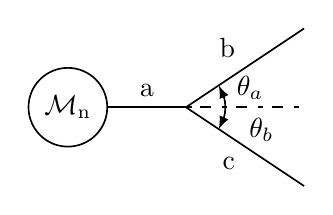
\begin{tikzpicture}[>=latex, line width=0.6pt,]
		\node[draw,circle, minimum size=1cm, inner sep=2pt] (rest) at (-1,0) {\(\mathcal{M}_\mathrm{n}\)};
		\coordinate (splitPoint) at (0.5, 0);
		\coordinate (continual) at (2,0);
		\coordinate (splitUp) at (2, 1);
		\coordinate (splitDown) at (2, -1);
		\draw (rest) to [edge label=a] (splitPoint);
		\path[draw, dash pattern=on 2pt off 3pt on 4pt off 4pt] (splitPoint) -- (continual);
		\path[draw] (splitPoint) to [edge label=b] (splitUp);
		\path[draw] (splitPoint)  to [edge label'=c] (splitDown);

		\pic[draw, "\(\theta_a\)",  ->, angle eccentricity=1.7] {angle = continual--splitPoint--splitUp};
		\pic[draw, "\(\theta_b\)",  <-, angle eccentricity=2.] {angle = splitDown--splitPoint--continual};
	\end{tikzpicture}
	\hspace{1cm}
	\begin{tikzpicture}[>=latex, line width=0.6pt]
		%\node[draw,circle, minimum size=1cm, inner sep=2pt, pattern=north west lines] (rest) at (-1,0) { };
		\coordinate (incoming) at (-1, 0);
		\coordinate (splitPoint) at (0.5, 0);
		\coordinate (continual) at (2,0);
		\node[draw,circle, minimum size=1cm, inner sep=2pt] (rest) at (2,1) {\(\mathcal{M}_\mathrm{n}\)};
		\coordinate (splitDown) at (2, -1);
		\draw (incoming) to [edge label=a] (splitPoint);
		\path[draw, dash pattern=on 2pt off 3pt on 4pt off 4pt] (splitPoint) -- (continual);
		\path[draw] (splitPoint) to [edge label=b] (rest);
		\path[draw] (splitPoint)  to [edge label'=c] (splitDown);

		\pic[draw, "\(\theta_a\)",  ->, angle eccentricity=1.7] {angle = continual--splitPoint--splitUp};
		\pic[draw, "\(\theta_b\)",  <-, angle eccentricity=2.] {angle = splitDown--splitPoint--continual};
	\end{tikzpicture}
	\caption{Kinematics of timelike (left) vs spacelike (right) parton branching.}
	\label{fig:splitKinematics}
\end{figure}

Consider nearly collinear timelike splitting of a parton, \(a\to b+c\) shown in Fig.~\ref{fig:splitKinematics}. Let's assume the partons are massless, and define the evolution scale (\(t\)) as,
\begin{align}
	t \equiv p_a^2 \approx 2E_bE_c(1 - \cos\theta)  \approx z(1-z)E_a^2\theta^2
\end{align}
Where, \(z = E_b/E_a = 1 - E_c/E_a\) and \(\theta = \theta_a + \theta_b\) is the small opening angle.  The cross-section of a \(n\)-parton state branching into \(n+1\)-parton state~\cite{Ellis_Stirling_Webber_1996}
%processes can be calculated by considering \(n\)-parton matrix element.
%\begin{equation}
%	\label{eq:nPartonXsec}
%	d\sigma_n = \mathcal{F}|\mathcal{M}_n|^2d\mathbf{\Phi}_n
%\end{equation}
%
%Where \(\mathcal{F}\) is the initial-state flux factor and \(\mathbf{\Phi}_n\) is phase space of the \(n\)-parton final state. In the branching process the \(n\)-parton pre-split phase space volume element:
%
%\begin{equation}
%	d\mathbf{\Phi}_{n} = \ldots \frac{d^3\mathbf{p}_a}{2(2\pi)^3E_a}
%\end{equation}
%
%will be replaced by the \(n+1\)-parton phase space and the \(n+1\)-parton matrix element can be calculated from the \(n\)-parton matrix element. 
%\begin{align}
%	d\mathbf{\Phi}_{n+1} &= \ldots \frac{d^3\mathbf{p}_b}{2(2\pi)^3E_b} \frac{d^3\mathbf{p}_c}{2(2\pi)^3E_c} 
%	= d\mathbf{\Phi}_{n} \frac{1}{4(2\pi)^3}dtdzd\phi \notag\\
%	|\mathcal{M}_{n+1}\big|^2 &\sim \frac{8\pi\alpha_s}{t}CF|\mathcal{M}_n|^2
%\end{align}
%
%Substituting in Eq.~\ref{eq:nPartonXsec} and integrating away the \(d\phi\), we get,
%
\begin{table}[htbp]
	\centering
	\setlength{\tabcolsep}{6pt}
	\renewcommand{\arraystretch}{1.6}
	\begin{tabular}{
		>{\centering\arraybackslash}m{2cm}
		>{\centering\arraybackslash}m{4.0cm}
		>{\raggedright\arraybackslash}m{8cm}
		}
		\toprule
		Kernel (\(ij\)) & Diagram                                                             & \(\hat{P}_{ij}(z)\) \\
		\midrule
		\(qq\)          & \splitvertex{fermion}{q}{}{fermion}{q}{z}{gluon}{g}{1-z}            &
		\(\displaystyle C_F\left[\frac{1+z^2}{1-z}\right]\)                                                         \\
		\(gq\)          & \splitvertex{fermion}{q}{}{gluon}{g}{z}{fermion}{q}{1-z}            &
		\(\displaystyle C_F\,\frac{1+(1-z)^2}{z}\)                                                                  \\
		\(qg\)          & \splitvertex{gluon}{g}{}{fermion}{q}{z}{anti fermion}{\bar{q}}{1-z} &
		\(\displaystyle T_R\left[z^2 + (1-z)^2\right]\)                                                             \\
		\(gg\)          & \splitvertex{gluon}{g}{}{gluon}{g}{z}{gluon}{g}{1-z}                &
		\(\displaystyle C_A\left[\frac{z}{1-z} + \frac{1-z}{z} + z(1-z)\right] \)                                   \\
		\bottomrule
	\end{tabular}
	\caption[Leading-order DGLAP splitting functions and their diagrams]{%
		The four leading-order collinear splittings entering the DGLAP evolution
		of Eq.~\ref{eq:xsecBranching}. The daughter parton \(i\) carrying momentum
		fraction \(z\) is drawn on the upper leg, the recoiling parton \((1-z)\)
		on the lower~\cite{Ellis_Stirling_Webber_1996}.}
	\label{tab:splitfns}
\end{table}
\begin{align}
	\label{eq:xsecBranching}
	%d\sigma_{n+1} &= d\sigma_n \frac{dt}{t}dz\frac{\alpha_s}{2\pi}\int\frac{d\phi}{2\pi}CF \notag\\
	d\sigma_{n+1} & = d\sigma_n \frac{dt}{t}dz\frac{\alpha_s}{2\pi} \hat{P}_{ba}
\end{align}

The \(\hat{P}_{ba}(z)\) are the \emph{unregularized Altarelli--Parisi splitting functions}, giving the probability of the branching \(a \to b + c\) with \(b\) taking a fraction \(z\) of \(a\)'s energy.
%
Their leading order forms are shown in Tab.~\ref{tab:splitfns}.
%
\(\hat{P}_{qq}\) diverges as \(z\to1\), \(\hat{P}_{gq}\) as \(z\to0\), and \(\hat{P}_{gg}\) at both ends, each of these limits being the emission of a soft gluon.
%
Only \(\hat{P}_{qg}\), the splitting of a gluon into a \(q\bar{q}\) pair, stays finite over the whole range of \(z\).
%
%This soft pole is what grooming procedures like SoftDrop (Sec.~\ref{sec:jetAlgo}) are built to remove from a measured jet.

Same equation would hold for the space-like case.
%
To obtain the evolution equations, we can frame the evolution in terms of the change in parton distribution function \(f(x,t)\) when the evolution scale \(t\) goes from \(t\) to \(t+\delta t\),
%
\begin{align}
	\delta f_i(x, t) & = \delta f_\mathrm{in} - \delta f_\mathrm{out} \notag                                                                                     \\
	                 & =\frac{\delta t}{t} \sum_j \int_{0}^{1} dz \frac{\alpha_s}{2\pi} \left[\frac{\hat{P}_{ij}(z)}{z}f_j(x/z, t) - \hat{P}_{ji}f_i(x,t)\right]
\end{align}
%
The second term of the RHS gives \emph{Sudakov form factor}, which gives the probability of a parton \(i\) evolving from scale \(t\) to a softer scale \(t_0\) without a resolvable emission,
%
\begin{align}
	\Delta_i(t) \equiv \exp(-\sum_j\int_{t_0}^{t} \frac{dt^\prime}{t^\prime}\int dz\frac{\alpha_s}{2\pi} \hat{P}_{ji}(z))
\end{align}

We get the familiar DGLAP-like evolution equations,

\begin{align}
	t\frac{\partial}{\partial t}\left(\frac{f_i}{\Delta_i}\right) = \frac{1}{\Delta_i}\sum_j \int \frac{dz}{z}\frac{\alpha_s}{2\pi}
	\hat{P}_{ij}(z)f_j(x/z, t)\end{align}


To deal with singularities corresponding to soft gluons at \(z\to 1\), we introduce an explicit infrared cut-off \(z < 1-\epsilon(t)\) .  Requiring the transverse momentum in timelike branching \(a\to bc\) to be positive,
\begin{align}
	p_T^2    & = z(1-z)p_a^2 - (1-z)p_b^2 - zp_c^2 > 0 \notag \\
	\implies & z(1-z) > t_0/t \implies t_0/t < z < 1 - t_0/t
	%	\implies&  z, 1-z > \epsilon(t) = \frac{1 - \sqrt{1-4t/t_0}}{2}\simeq t_0/t \notag\\
\end{align}
and also, \(t > 2t_0\). Thus the Sudakov factors become,
%
\begin{align}
	\Delta_i(t) \equiv \exp(-\sum_j\int_{2t_0}^{t}
	\frac{dt^\prime}{t^\prime}
	\int_{t_0/t^\prime}^{1-t_0/t^\prime} dz
	\frac{\alpha_s}{2\pi} \hat{P}_{ji}(z))
	\label{eq:col`inearSudakov}
\end{align}

\subsection{Angular Ordering}
\label{sec:angularOrdering}
Sec.~\ref{subsec:dglap} took collinear enhancements into account to all orders in
\(\alpha_s\). However it does not take the enhancement in soft gluon emission at wide emission angle.
This is demonstrated in Eq.~\ref{eq:softPropagator} by considering an on-mass-shell external line of
momentum \(p\), mass \(m\) emitting a gluon with momentum \(q\)  at an angle \(\theta\)
\begin{equation}
	\frac{1}{(p\pm q)^2 - m^2} = \frac{\pm1}{2p\cdot q}
	= \frac{\pm1}{2\omega E(1-v\cos\theta)},
	\label{eq:softPropagator}
\end{equation}
where \(\omega\) is the gluon energy, \(E\) and \(v\) the energy and velocity of the
emitter and \(\theta\) the emission angle. For light partons \(v\to1\) and the
collinear enhancement appears as \(\theta\to0\); the enhancement as \(\omega\to0\)
holds for any velocity and angle. Internal lines  are off-mass-shell and carry no such enhancement, since
\((p+q)^2-m^2\to p^2-m^2\neq0\). The cross section carries a sum over all pairs of external lines \(\{i,j\}\),
\begin{align}
	\label{eq:antennaSplitXSec}
	d\sigma_{n+1} & = d\sigma_n\,\frac{d\omega}{\omega}\frac{d\Omega}{2\pi}
	\frac{\alpha_s}{2\pi}\sum_{i,j}C_{ij}W_{ij}
\end{align}
The weighted sum \(\sum_{i,j}C_{ij}W_{ij}\)  is called the \emph{antenna pattern} of the process. The \emph{color factor} \(C_{ij}\) and \emph{radiation function} \(W_{ij}\)  are defined as,
\begin{align}
	C_{ij} & = -\mathbf{Q}_i\cdot\mathbf{Q}_j  \notag               \\
	W_{ij} & = \frac{\omega^2 p_i\cdot p_j}{p_i\cdot q\;p_j\cdot q}
	= \frac{1-v_iv_j\cos\theta_{ij}}
	{(1-v_i\cos\theta_{iq})(1-v_j\cos\theta_{jq})}
\end{align}
The vectors \(\mathbf{Q}_{i}\) represents color charge of parton \(i\).
%\(\mathbf{Q}_i^2 = C_F\) for a quark, \(C_A\) for a gluon and \(0\) for a color singlet. 
\begin{equation}
	\mathbf{Q}_i^2 =
	\begin{cases}
		C_F = 4/3 & i \in \text{quarks}        \\[-15pt]
		C_A = 3   & i \in \text{gluons}        \\[-15pt]
		0         & i \in \text{color singlet}
	\end{cases}
\end{equation}

\(W_{ij}\) comes from interference between lines \(i\) and \(j\). \(W_{ij}\) can be separated into two parts  \(W^{[i/j]}_{ij}\) each with an \emph{incoherent} and a \emph{coherent} contribution from line \(i/j\)  . Assuming massless emitters (\(v_i=v_j=1\)) for simplicity,
\begin{align}
	W_{ij}       & = W^{[i]}_{ij} + W^{[j]}_{ij}\notag                                                                                                                                                                         \\
	W^{[i]}_{ij} & = \frac{1}{2}\left(\overbrace{\frac{1}{1-\cos\theta_{iq}}}^\mathrm{incoherent} + \overbrace{\frac{\cos\theta_{iq}-\cos\theta_{ij}}{(1-\cos\theta_{jq}) (1-\cos\theta_{iq})}}^\mathrm{coherent}\right)\notag \\
	             & =  \frac{1}{2(1-\cos\theta_{iq})}\left(1 + \frac{\cos\theta_{iq}-\cos\theta_{ij}}{1-\cos\theta_{ij}\cos\theta_{iq} - \sin\theta_{ij}\sin\theta_{iq}\cos\phi_{iq}}\right)
	\label{eq:antennaSplit}
\end{align}
Using the direction of line \(i\) as the z-axis, \(d\Omega \)  from Eq.~\ref{eq:antennaSplitXSec} becomes \(d\cos\theta_{iq}\,d\phi_{iq}\), We can carry out the \(\phi_{iq}\) integration,
\begin{align}
	\int_0^{2\pi}\frac{d\phi_{iq}}{2\pi}W^{[i]}_{ij} & = \frac{1}{1-\cos\theta_{iq}}\left(\frac{1 + \frac{\cos\theta_{iq}-\cos\theta_{ij}}{|\cos\theta_{iq}-\cos\theta_{ij}|}}{2}\right) \notag \\
	                                                 & = \begin{cases}
		                                                     \dfrac{1}{1-\cos\theta_{iq}} & \cos\theta_{iq} > \cos\theta_{ij} \implies \theta_{iq} < \theta_{ij} \\[-10pt]
		                                                     0                            & \text{otherwise,}
	                                                     \end{cases}
	\label{eq:angularOrdering}
\end{align}

Eq.~\ref{eq:angularOrdering}  shows that azimuth-averaged soft gluon emission from a line \(i\) is confined to a cone, centered on \(i\)'s direction, extending up to the direction of line \(j\), \(i\)'s sibling from the preceding split.
%
Since the emission probability of Eq.~\ref{eq:antennaSplitXSec} is weighted by the color charges, a gluon radiates \(C_A/C_F = 9/4\) times as much as a quark of the same energy into the same cone.
%
Gluon jets are therefore wider and carry more particles than quark jets of the same momentum, a difference the classifiers of App.~\ref{app:ML} are trained to pick up, and one that has to be kept in mind whenever angularities are compared between samples with different quark and gluon fractions.
%The total soft gluon emission cross-section can be then easily obtained for two external lines forming a color singlet (\(e^+e^-\to q\bar{q}\)) have \(\mathbf{Q}_i+\mathbf{Q}_j=0\) and hence \(C_{q\bar{q}}=\mathbf{Q}_q^2=\mathbf{Q}_{\bar{q}}^2 = C_F\), and angular ordering suppresses radiation outside the cones extending from \(q\) to \(\bar{q}\) and vice versa.

%\begin{align}
%	d\sigma_{q\bar{q}g}& = d\sigma_{q\bar{q}}\frac{\Theta(\cos(\theta_{qg})-\cos(\theta_{q\bar{q}}))}{1-\cos\theta_{qg}}d(\cos\theta_{qg})\frac{\alpha_s}{2\pi}\frac{d\omega}{\omega}C_F
%	\label{eq:qqbarSinglet}
%\end{align}
%We will come back to Eq.~\ref{eq:qqbarSinglet} 

\subsection{Color Coherence}
\label{sec:colorCoherence}
Lets take the case of three partons \(\{i,j,k\}\) forming a color singlet (\(\mathbf{Q}_i + \mathbf{Q}_j +\mathbf{Q}_k = 0\)) e.g., \(e^+e^-\to q\bar{q} g\). First, partons \(l\) and \(k\) come from a color singlet state (\(\mathbf{Q}_l +\mathbf{Q}_k = 0\)). Then \(l\) splits into \(i\) and \(j\) (\(\mathbf{Q}_l = \mathbf{Q}_i + \mathbf{Q}_j = -\mathbf{Q}_k\)). The antennae function for this state is:
\begin{align}
	\label{eq:threePartonW}
	\sum_{a,b}C_{ab}W_{ab} & = -\mathbf{Q}_i\!\cdot\!\mathbf{Q}_jW_{ij} -\mathbf{Q}_j\!\cdot\!\mathbf{Q}_kW_{jk} -\mathbf{Q}_i\!\cdot\!\mathbf{Q}_kW_{ik} \notag                                                   \\
	                       & = \frac{1}{2}\left[\mathbf{Q}_i^2(W_{ij} + W_{ik} - W_{jk}) + \mathbf{Q}_j^2(W_{ij} + W_{jk} - W_{ik}) + \mathbf{Q}_k^2(W_{ik} + W_{jk} - W_{ij})\right]\notag                        \\
	                       & =\mathbf{Q}_i^2\left(W_{ij}^{[i]} + \tilde{W}_{jk}^{[i]} - \tilde{W}_{ik}^{[j]}\right) + \mathbf{Q}_j^2\left(W_{ij}^{[j]} + \tilde{W}_{ik}^{[j]} - \tilde{W}_{jk}^{[i]}\right) \notag \\
	                       & + \mathbf{Q}_k^2\left(\tilde{W}_{jk}^{[i]} + \tilde{W}_{ik}^{[j]} + \frac{W_{ik}^{[k]} + W_{jk}^{[k]} }{2}\right)
\end{align}
Where,
\begin{equation}
	\tilde{W}_{jk}^{[i]} = \frac{W^{[i]}_{ik} - W^{[i]}_{ij}}{2},\quad \tilde{W}_{ik}^{[j]} = \frac{W^{[j]}_{jk} - W^{[j]}_{ij}}{2}
\end{equation}
are shifted radiation functions for lines \(i\) and \(j\), with the collinear singularity canceled out. This allows us to make certain useful approximations. Taking \(\theta_{ij}\to0\), we can approximate the directions of \(i\) and \(j\) by \(l\).
\begin{align}
	W_{ik}^{[k]} \simeq W_{jk}^{[k]} \simeq W_{lk}^{[k]},\text{and}~\tilde{W}_{jk}^{[i]} \simeq \tilde{W}_{ik}^{[j]} \simeq W_{lk}^{[ij]}/2
\end{align}
Where,
\begin{equation}
	\tilde{W}^{[ij]}_{lk} = \begin{cases}
		W^{[l]}_{lk} & \theta_{lq}>\theta_{ij}  \\[-10pt]
		0            & \theta_{lq}<\theta_{ij},
	\end{cases}
\end{equation}
\begin{equation}
	W \simeq \mathbf{Q}_i^2W^{[i]}_{ij} + \mathbf{Q}_j^2W^{[j]}_{ij}
	+ \mathbf{Q}_k^2W^{[k]}_{lk} + \mathbf{Q}_l^2\tilde{W}^{[ij]}_{lk},
	\label{eq:coherentPattern}
\end{equation}

\begin{figure}[htbp]
	\centering
	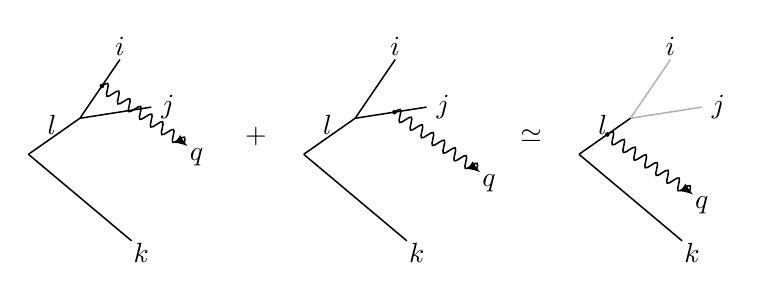
\begin{tikzpicture}[line width=0.55pt, scale=0.76,
			gl/.style={decorate, decoration={coil, aspect=0, segment length=1.7mm,
							amplitude=0.7mm}, ->}]

		\begin{scope}[xshift=0cm]
			\coordinate (o) at (0,0);
			\coordinate (l) at (35:1.05);
			\coordinate (i) at (46:2.2);
			\coordinate (j) at (21:2.2);
			\coordinate (k) at (-40:2.25);
			\draw[black] (l) -- (i) node[black, above=-2pt] {\(i\)};
			\draw[black] (l) -- (j) node[black, right=0pt] {\(j\)};
			\draw (o) -- node[above left=-5pt, pos=0.55] {\(l\)} (l);
			\draw (o) -- (k) node[below right=-4pt] {\(k\)};
			\coordinate (e) at ($(l)!0.55!(i)$);
			\fill (e) circle (1.1pt);
			\draw[gl] (e) -- ($(e)+(-35:1.75)$) node[below right=-4pt] {\(q\)};
			%\node at (1.1,-2.1) {\(\mathcal{M}_i\)};
		\end{scope}

		\node at (3.8,0.3) {\(+\)};

		\begin{scope}[xshift=4.6cm]
			\coordinate (o) at (0,0);
			\coordinate (l) at (35:1.05);
			\coordinate (i) at (46:2.2);
			\coordinate (j) at (21:2.2);
			\coordinate (k) at (-40:2.25);
			\draw[black] (l) -- (i) node[black, above=-2pt] {\(i\)};
			\draw[black] (l) -- (j) node[black, right=0pt] {\(j\)};
			\draw (o) -- node[above left=-5pt, pos=0.55] {\(l\)} (l);
			\draw (o) -- (k) node[below right=-4pt] {\(k\)};
			\coordinate (e) at ($(l)!0.55!(j)$);
			\fill (e) circle (1.1pt);
			\draw[gl] (e) -- ($(e)+(-35:1.75)$) node[below right=-4pt] {\(q\)};
			%\node at (1.1,-2.1) {\(\mathcal{M}_j\)};
		\end{scope}

		\node at (8.4,0.3) {\(\simeq\)};

		\begin{scope}[xshift=9.2cm]
			\coordinate (o) at (0,0);
			\coordinate (l) at (35:1.05);
			\coordinate (i) at (46:2.2);
			\coordinate (j) at (21:2.2);
			\coordinate (k) at (-40:2.25);
			\draw[black!30] (l) -- (i) node[black, above=-2pt] {\(i\)};
			\draw[black!30] (l) -- (j) node[black, right=0pt] {\(j\)};
			\draw (o) -- node[above left=-5pt, pos=0.55] {\(l\)} (l);
			\draw (o) -- (k) node[below right=-4pt] {\(k\)};
			\coordinate (e) at ($(o)!0.55!(l)$);
			\fill (e) circle (1.1pt);
			\draw[gl] (e) -- ($(e)+(-35:1.75)$) node[below right=-4pt] {\(q\)};
			%\node at (1.1,-2.1) {\(\mathcal{M}_l\)};
		\end{scope}
	\end{tikzpicture}
	\caption{Wide-angle emission of soft gluon \(q\), off \(i\) and \(j\), acts as if
		the emission came off the parent parton \(l\), imagined to be on shell.}
	\label{fig:threeParton}
\end{figure}


Each parton radiates in proportion to its color charge squared. When \(i\) and \(j\) close in angle their incoherent
contributions are limited to cones of half-angle \(\theta_{ij}\), while at larger
angles, out to the direction of \(k\), they radiate coherently in proportion to
their combined charge \(\mathbf{Q}_l^2\), as if from an internal line of momentum
\(p_l = p_i+p_j\) as shown in Fig.~\ref{fig:threeParton}.

\subsection{Coherent Parton Branching}
\label{sec:coherentPartonBranching}
Extended to higher orders this gives a \emph{coherent parton branching} formalism.
In place of the virtual mass-squared \(t\) the evolution variable is the opening
angle, or more precisely
\begin{equation}
	\zeta = \frac{p_b\cdot p_c}{E_bE_c} \simeq 1-\cos\theta
	\label{eq:zeta}
\end{equation}
for \(a\to bc\), with angular ordering \(\zeta^\prime<\zeta\) imposed on successive
branchings and the propagator factor \(dt/t\) of Sec.~\ref{subsec:dglap} replaced by
\(d\zeta/\zeta\). Using the splitting function \(\hat{P}_{ba}(z)dz\) rather than the
soft approximation \(\mathbf{Q}_a^2d\omega/\omega\) treats both soft and collinear
enhancements correctly, so that
\begin{equation}
	d\sigma_{n+1} = d\sigma_n\,\frac{d\zeta}{\zeta}\,dz\,
	\frac{\alpha_s}{2\pi}\hat{P}_{ba}(z).
	\label{eq:coherentBranching}
\end{equation}
The virtual mass-squared cut-off is replaced by an angular one,
\(\zeta_0 = t_0/E^2\) for a parton of energy \(E\), and the convenient evolution
variable \(\tilde{t} = E^2\zeta \geq t_0\) in terms of which the ordering condition \(\zeta_b,\zeta_c<\zeta_a\) and the
resulting cut-off on \(z\) read
\begin{equation}
	\tilde{t}_b < z^2\tilde{t},
	\qquad
	\tilde{t}_c < (1-z)^2\tilde{t},
	\qquad
	\sqrt{t_0/\tilde{t}} < z < 1-\sqrt{t_0/\tilde{t}} ,
	\label{eq:orderingCutoff}
\end{equation}
with \(\tilde{t}=\tilde{t}_a\) and \(z=E_b/E_a\). Neglecting the masses of \(b\) and
\(c\),
\begin{equation}
	t = z(1-z)\tilde{t},
	\qquad
	p_t^2 = z^2(1-z)^2\tilde{t},
	\label{eq:tAndPt}
\end{equation}
and the Sudakov form factor of Sec.~\ref{subsec:dglap} becomes
\begin{align}
	\tilde{\Delta}_i(\tilde{t}) \equiv \exp(-\sum_j\int_{4t_0}^{\tilde{t}}
	\frac{d\tilde{t}^\prime}{\tilde{t}^\prime}
	\int_{\sqrt{t_0/\tilde{t}^\prime}}^{1-\sqrt{t_0/\tilde{t}^\prime}} dz
	\frac{\alpha_s(z^2(1-z)^2\tilde{t}^\prime)}{2\pi} \hat{P}_{ji}(z))
	\label{eq:coherentSudakov}
\end{align}

At large \(\tilde{t}\) this falls more slowly than its collinear counterpart, though
still faster than any negative power of \(\tilde{t}\). The slower fall implies less
branching, which is the suppression of soft gluon emission by angular ordering.

\subsection{Angular structure of a jet}
\label{sec:angularityEstimate}
Sec.~\ref{sec:coherentPartonBranching} is enough to estimate what the radiation around a hard parton looks like.
%
At a hadron collider, the angle \(\theta\) between two particles is measured as their distance \(\Delta R\) in the \etaphi plane and the energy \(E\) as the transverse momentum \(p_\mathrm{T}\) (see Sec.~\ref{sec:detCoordSys}), and a \emph{jet} is, for now, all the radiation within \(\Delta R < R\) of the initiating parton.
%
Taking \(z\) to be the momentum fraction of the emitted gluon, as in \(\hat{P}_{gq}\) and \(\hat{P}_{gg}\) of Tab.~\ref{tab:splitfns}, the soft limit is \(\hat{P}_{gi}(z) \to 2C_i/z\) and \(d\zeta/\zeta \to 2d\theta/\theta\), so Eq.~\ref{eq:coherentBranching} becomes,
\begin{equation}
	dP = \frac{2\alpha_s C_i}{\pi}\frac{d\hat{\theta}}{\hat{\theta}}\frac{dz}{z}, \qquad \hat{\theta} \equiv \frac{\Delta R}{R} < 1
	\label{eq:lundDensity}
\end{equation}
Where, \(C_i = \mathbf{Q}_i^2\) is the color charge of the initiating parton from Sec.~\ref{sec:angularOrdering}.
%
Eq.~\ref{eq:lundDensity} is flat in \(\ln(1/z)\) and \(\ln(1/\hat{\theta})\), so a jet is filled uniformly in this plane, the \emph{Lund plane}, down to the cut-off.
%
The \emph{generalized angularity} of a jet is the sum over its emissions,
\begin{equation}
	\lambda_\beta = \sum_{i \in \mathrm{jet}} z_i\,\hat{\theta}_i^{\,\beta}
	\label{eq:angularityShower}
\end{equation}
Eq.~\ref{eq:LambdaKappaBeta} is the same quantity written in terms of the measured constituents of a jet, with \(z_i \to p_\mathrm{T, const}/p_\mathrm{T, jet}\) and \(\hat{\theta}_i \to \Delta R_\mathrm{const, jet}/R\), and with a second exponent \(\kappa\) on \(z_i\) which is \(1\) here.
%
For \(\beta > 0\), an emission contributes nothing to \(\lambda_\beta\) in either the soft or the collinear limit, which is what makes it an IRC safe observable.
%
Since \(\lambda_\beta\) is additive, the probability of a jet having an angularity below \(\hat{\lambda}_\beta\) is the probability of no emission with \(z\hat{\theta}^\beta > \hat{\lambda}_\beta\), which is the Sudakov form factor of Eq.~\ref{eq:coherentSudakov} with the no-emission condition replaced accordingly.
%
Calling this cumulative distribution \(\Sigma_i(\hat{\lambda}_\beta)\), with the hat marking it as a parton level quantity like in Eq.~\ref{eq:factorization}, the hadron level cross section follows from it through the fragmentation function of Eq.~\ref{eq:factorization} for \(\mathbf{O} = \lambda_\beta\), summed over the flavor of the parton initiating the jet,
\begin{align}
	\frac{d\sigma}{d\lambda_\beta} & = \sum_{i \in \{q, g\}}\int d\hat{\lambda}_\beta\,\frac{d\sigma_i}{d\hat{\lambda}_\beta}\,D_i(\hat{\lambda}_\beta \to \lambda_\beta) = \sum_{i \in \{q, g\}}\sigma_i\int d\hat{\lambda}_\beta\,\frac{d\Sigma_i}{d\hat{\lambda}_\beta}\,D_i(\hat{\lambda}_\beta \to \lambda_\beta)
	\label{eq:angularityCumulant}
\end{align}
Where, \(\sigma_i\) is the cross section for producing a jet initiated by parton \(i\), i.e. Eq.~\ref{eq:factorization} with everything but the flavor of the outgoing parton integrated over, and \(d\sigma_i/d\hat{\lambda}_\beta = \sigma_i\,d\Sigma_i/d\hat{\lambda}_\beta\) is its parton level distribution.
%
Normalized to the total cross section, the left hand side is the distribution measured in Ch.~\ref{ch:angularities}.
%
The rest of this section is about \(\Sigma_i\), and comes back to \(D_i\) at the end.
%
At fixed coupling,
\begin{align}
	\Sigma_i(\hat{\lambda}_\beta) & = \exp\left(-\frac{2\alpha_s C_i}{\pi}\int_0^1\frac{d\hat{\theta}}{\hat{\theta}}\int_0^1\frac{dz}{z}\,\Theta(z\hat{\theta}^\beta - \hat{\lambda}_\beta)\right) \notag \\
	                              & = \exp\left(-\frac{\alpha_s C_i}{\pi\beta}\ln^2\hat{\lambda}_\beta\right)
	\label{eq:angularitySudakov}
\end{align}
Quark and gluon jets differ only through \(C_i\), so \(\Sigma_g = \Sigma_q^{C_A/C_F}\)~\cite{Larkoski_2014}.
%
A convenient choice for scale of \(\alpha_s\) is \(p_\mathrm{T, jet}R\), the largest transverse momentum an emission inside the jet can have.
%

Tab.~\ref{tab:angularityEstimate} evaluates Eq.~\ref{eq:angularitySudakov} for the three \(\beta\) values measured in Ch.~\ref{ch:angularities}.

\begin{table}[htbp]
	\centering
	\begin{tabular}{c c c c c}
		\toprule
		\multirow{2}{*}{\(\beta\)} & \multicolumn{2}{c}{median \(\hat{\lambda}_\beta\)} & \multicolumn{2}{c}{fraction with \(\hat{\lambda}_\beta > 0.1\)}                 \\
		\cmidrule(lr){2-3} \cmidrule(lr){4-5}
		                           & quark                                              & gluon                                                           & quark & gluon \\
		\midrule
		0.5                        & 0.13                                               & 0.26                                                            & 59\%  & 87\%  \\
		1                          & 0.06                                               & 0.15                                                            & 36\%  & 64\%  \\
		2                          & 0.02                                               & 0.07                                                            & 20\%  & 40\%  \\
		\bottomrule
	\end{tabular}
	\caption[Leading logarithmic estimates of jet angularities at RHIC]{Parton level median angularity and fraction of jets with \(\hat{\lambda}_\beta > 0.1\) from Eq.~\ref{eq:angularitySudakov} at \(\alpha_s = 0.2\), corresponding to \(p_\mathrm{T, jet} \approx 20~\mathrm{GeV}/c\) and \(R = 0.4\), for quark (\(C_F = 4/3\)) and gluon (\(C_A = 3\)) initiated jets.}
	\label{tab:angularityEstimate}
\end{table}

Median angularities are larger by  a factor of 2--3 for gluon jets compared to quark jets.
%
Increasing \(\beta\) pushes both to smaller values and widens the gap between them, as the observable weighs the wide angle radiation more heavily.
%
Going up in \(p_\mathrm{T, jet}\) only changes \(\alpha_s\) logarithmically, so the distributions are expected to narrow slowly.

%Eq.~\ref{eq:lundDensity} only holds for emissions whose transverse momentum, \(k_\mathrm{T} \approx z\,p_\mathrm{T, jet}\Delta R\), is above the scale where \(\alpha_s\) stops being perturbative, and below it the emissions are replaced by hadronization, which is what \(D_i\) in Eq.~\ref{eq:angularityCumulant} accounts for. 
%%
%An emission with \(k_\mathrm{T}\) between \(\Lambda \approx 0.2\)~GeV and \(1\)~GeV sitting at the edge of the jet contributes \(k_\mathrm{T}/(p_\mathrm{T, jet}R) \approx 0.03\)--\(0.12\) to \(\lambda_\beta\) for any \(\beta\), which is as large as the medians of Tab.~\ref{tab:angularityEstimate}. 
%%
%Thus at RHIC energies the npQCD part of an angularity is not a small correction on top of the pQCD part, and it only falls as \(1/p_\mathrm{T, jet}\). 
%%
%This is why the angularity distributions measured in Ch.~\ref{ch:angularities} sit above these estimates by about this much, why removing the soft wide angle radiation by grooming (Sec.~\ref{sec:jetAlgo}) brings them closer, and why the event generators of Sec.~\ref{sec:eventGenerators} are tested there as much on their hadronization as on their showers. 
%
%These are leading logarithmic estimates at fixed coupling, and are indicative rather than predictions. 
%%
%Terms of order \(\alpha_s\ln(1/\lambda_\beta)\), coming from the running of \(\alpha_s\), hard collinear splittings, the recoil of the jet axis against the emissions for \(\beta \leq 1\), and radiation across the jet boundary, are all of order one half at these values. 
%%
%The angularities with \(\kappa \neq 1\) used for \AuAu collisions in Ch.~\ref{ch:angularities} are not IRC safe, and no estimate of this kind exists for them. 

\chapter{Relativistic Kinematics}
\label{app:kinematics}
\section{Laboratory vs Center-of-mass frames}
A typical collision is a two-to-many reaction like:
\begin{equation}
	\underbrace{A}_{\rm projectile} + \underbrace{B}_{\rm target} \rightarrow C_1 + C_2 + C_3 + \ldots,
\end{equation}

In \emph{laboratory frame}, the target is at rest, so,
\begin{equation}
	\mathbf{p}_B^{\rm lab} = \vec{0} \implies p_{B}^{\rm lab} = (m_B, 0, 0, 0),
\end{equation}

In \emph{center-of-mass} frame, the sum of three-momentum vectors vanish in the initial and final states
\begin{equation}
	\mathbf{p}_A^{\rm cm} + \mathbf{p}_B^{\rm cm} =\sum_i \mathbf{p}_{C, i}^{\rm cm} = \vec{0},
\end{equation}

Using Lorentz invariance of the Mandelstam variable \(s \equiv (p_A + p_B)_\mu(p_A + p_B)^\mu\):
\begin{align}
	s &= (E^{\rm lab}_A + m_B)^2 - |\mathbf{p}^{\rm lab}_A|^2 = (E^{\rm cm}_A + E^{\rm cm}_B)^2 \notag \\
	\implies s &= m_A^2 + m_B^2  + 2m_BE^{\rm lab}_A = (E^{\rm cm})^2 
\end{align}

As relativistic energies (\(\mathcal{O}(10^{2-3} \mathrm{GeV})\)) are much higher than reactant masses \(\mathcal{O}(1-10 \mathrm{GeV})\), 

\begin{equation}
	\sqrt{s} = E^{\rm cm} \approx \sqrt{2m_BE^{\rm lab}_A}
\end{equation}
As the center-of-mass energy that produces new particles increases only as \(\sqrt{E^{\rm lab}}\) , making any gain in particle production more expensive at relativistic energies. Thus modern colliders usually operate in center-of-mass frames.

\section{Coordinate system}
\label{sec:coordSysAppendix}
Considering the non-linear addition of velocities in relativistic mechanics,

\begin{equation}
	\beta = \frac{\beta_1 + \beta_2}{1 + \beta_1\beta_2},
\end{equation}

Considering the transformation \(y = \tanh^{-1}\beta\), 
\begin{align}
	\tanh^{-1}\beta_1 + \tanh^{-1}\beta_2 &= \tanh^{-1}  \frac{\beta_1 + \beta_2}{1 + \beta_1\beta_2} = \tanh^{-1}\beta\notag\\
	\implies y_1 + y_2 &= y
\end{align}

The addition is linear again.  We call this transformed velocity \emph{rapidity}, given by:
\begin{equation}
	y = \tanh^{-1}\beta = \frac{1}{2} \ln \frac{1 + \beta}{1 - \beta}  = \frac{1}{2} \ln \frac{E + p_z}{E - p_z}
	\label{eq:rapy}
\end{equation}

Rapidity can grow without bound, and at small velocities, \(y \approx \beta\), making it a relativistic analogue of velocity.  Since it transforms linearly under Lorentz boosts, rapidity distribution of particles retain their shapes. For relativistic energies, \(E \approx p\) , making Eq.~\ref{eq:rapy},
\begin{equation}
	y \approx  \frac{1}{2} \ln \frac{p + p_z}{p - p_z} = -\ln\left(\tan\frac{\theta}{2}\right) = \eta
\end{equation}
\(\eta\) is called the \emph{pseudo-rapidity}, the massless limit of rapidity. As shown in Fig.~\ref{fig:etavstheta}, pseudo-rapidity can be directly determined from particle production angle \(\theta\) measured with respect to the beam axis. 
\begin{figure}[htbp]
	\centering
	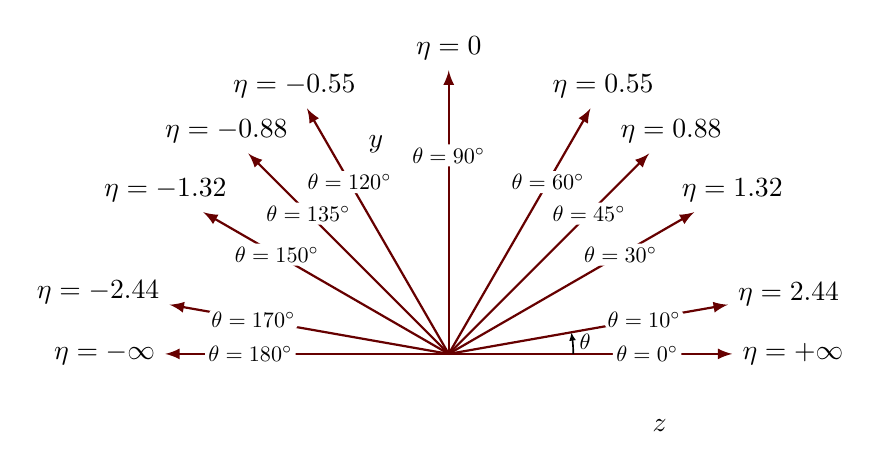
\begin{tikzpicture}[scale=3]
		%\message{^^JPseudorapidity including negative side}
		\pgfkeys{
			/pgf/fpu/output format=fixed, % fpu floating-point format
			/pgf/number format/precision=2 % two decimals
		}
		\def\R{1.2} % radius/length of lines
		\node[scale=1,below left=1] at (0,\R) {$y$}; % y axis
		\node[scale=1,below left=1] at (\R,0) {$z$}; % z axis
		\coordinate (O) at (0,0); % origin
		\foreach \t in {180,170,150,135,120,90,60,45,30,10,0}{ % loop over theta
			\ifnum \t = 0
			\def\e{+\infty} % infinity symbol
			\else \ifnum \t = 180
			\def\e{-\infty} % infinity symbol
			\else
			\pgfkeys{/pgf/fpu=true} % increase floating-point precision in computation
			\pgfmathparse{-ln(tan(\t/2))} % pseudorapidity
			\pgfkeys{/pgf/fpu=false} % turn off to avoid interference with following
			\pgfmathroundtozerofill{\pgfmathresult} % round with trailing zeroes
			\pgfmathsetmacro\e{\t==90?0:\pgfmathresult} % no trailing zeroes for theta = 0
			\fi \fi
			\message{^^Jt=\t, e=\e}
			\draw[eta line] % eta lines
			(O) -- (\t:\R) coordinate(P\t) node[anchor=180+\t,black] {$\eta=\e$}
			node[theta node] {$\theta=\t^\circ$};
		}
		\draw pic["$\theta$"scale=0.8,mysmallarrow] {angle = P0--O--P10}; % arrow label	
	\end{tikzpicture}
	\caption{Pseudorapidity \(\eta\) for several polar angles \(\theta\) measured from the beam (\(z\)) axis: \(\eta = 0\) perpendicular to the beam, and \(|\eta| \to \infty\) along it.}
	\label{fig:etavstheta}
\end{figure}

Also considering \emph{azimuthal angle} (\(\phi\)) and \emph{transverse-momentum} \(\left(p_{\rm T} = \sqrt{p_x^2 + p_y^2}\right)\) of the particles, which are invariant under boosts along the beam-line by design, we can use (\(p_{\rm T}, \eta, \phi\)) as the coordinate system for the particles produced in the collision. \Fref{fig:detcoords} illustrates this coordinate system for a cylindrical collider detector. 




\chapter{Event plane reconstruction}
\label{sec:EP_Recon}
The reaction plane, \(\Psi_{\rm RP}\) cannot be directly measured and is approximated by the second-order symmetry plane, $\Psi_{2,EP}$, referred to as the \emph{event plane}  in this text, for simplicity.  
%
\(\Psi_{\rm RP} \to \Psi_{2, EP}\) if nucleon distributions were in their average positions and devoid of fluctuations from interactions among nucleons~\cite{PhysRevC.101.064901}.
%
By measuring the charged particle azimuthal distribution, the n-th order event plane can be extracted by~\cite{Poskanzer:1998yz},  
%
\begin{equation}
	\Psi_{n,EP} = \frac{1}{n} \arctan \left(\frac{Q_{y, n}}{Q_{x, n}} \right),
	\label{eqn:EP}
\end{equation}
%
the weighted vector \(\mathbf{Q}_n = Q_{x, n}\hat{\mathbf{x}}+ Q_{y, n}\hat{\mathbf{y}}\) are given by,
%
\begin{align}
	\mathbf{Q}_n = \hat{\mathbf{x}}\sum_{\mathrm{tracks}} p_{\rm T, track} \cos (n \phi_{\rm track}) + \hat{\mathbf{y}}\sum_{\mathrm{tracks}} p_{\rm T, track} \sin (n \phi_{\rm track}).
	\label{Eqn:Qvecs}
\end{align}
%
where the sum is calculated for all reconstructed charged particles (tracks) in the event, $\phi_{\rm track}$ is the track's azimuthal angle, and $p_{\rm T, track}$ the track's transverse momentum.  
%

Due to finite acceptance and multiplicities, the calculated event plane has an underlying anisotropy that is corrected by applying two separate correction methods.  
%
First, a calibration and recentering correction procedures are applied to remove bias introduced by non-uniform acceptance of the TPC tracking system and further account for potential beam-condition effects~\cite{Barrette:1997pt,PhysRevC.55.1420,Poskanzer:1998yz}.  
%
This procedure involves recentering the weighted $\mathbf{Q}_2$-vectors such that, $\langle\mathbf{Q}_2 \rangle = \mathbf{0}$. 
%
It is done by calculating a modified $\mathbf{Q}_2$, obtained by subtracting an event averaged $\langle\mathbf{Q}_2 \rangle$ from each event's nominal $\mathbf{Q}_2$.
%

The higher harmonics of $\Psi_{n,EP}$ still persist after recentering \cite{Poskanzer:1998yz}, and are removed through a second correction step, referred to as  the shifting method, applied event-by-event  to make the event-plane angle isotropic in the lab frame \cite{Voloshin:2008dg}. 
%
This method defines a new angle:
%
\begin{equation}
	\Psi'_{2,EP} = \Psi_{2,EP} + \sum_n \frac{2}{n}
	(- \langle \sin (n\Psi_{2,EP}) \rangle \cos(n\Psi_{2,EP}) + \langle \cos(n\Psi_{2,EP}) \sin(n\Psi_{2,EP}) \rangle) ,
	\label{eqn:Shift}
\end{equation}
%
Usually 20 orders of Fourier moment are removed. 
%
Additional details of the recentering and shifting corrections can be found in Refs.~\cite{Wang:2012bga,Barrette:1997pt,Poskanzer:1998yz}

The difference between $\Psi_{RP}$ and \(\Psi_{2, EP}\) is quantified by event-plane resolution, $R_n$ or $R_n\{\Psi_{2, EP}\}$ given by Eqn.~\ref{resolution}. 
%
The observed $v_n$, $v_n^{\rm obs}$ is corrected for this limited resolution by doing, $v_n = v_{n}^{\rm obs}/R_n$ \cite{Abbas:2013taa,Poskanzer:1998yz}.  
%
\begin{equation}
	R_n = R_n\{\Psi_{2, EP}\} = \langle \cos(n[\Psi_{RP} - \Psi_{2, EP}]) \rangle \qquad \text{$n$ is even}
	\label{resolution}
\end{equation}

Furthermore, individual events are divided into two random sub-events by assigning charged tracks to sub-events, ``$a$" and ``$b$". 
%
The sub-events are unique, with approximately equal multiplicities. 
%
We can write the correlation of two event planes by taking the product of two sub-events, \cite{Barrette:1996rs,Poskanzer:1998yz}
%
\begin{equation}
	\langle \cos(n[\Psi_{2, EP}^{a} - \Psi_{2, EP}^{b}]) \rangle = 
	\langle \cos(n[\Psi_{2, EP}^{a} - \Psi_{RP}]) \rangle
	\langle \cos(n[\Psi_{2, EP}^{b} - \Psi_{RP}]) \rangle,
	\label{resolution2sub}
\end{equation}
%
This allows calculation of the event-plane resolution directly from data. Since $a$ and $b$ have equal multiplicities, the resolution of each sub-event can be calculated from the correlation between the two sub-events as \cite{Poskanzer:1998yz}:

\begin{equation}
	\langle \cos(n[\Psi_{2, EP}^{a} - \Psi_{RP}]) \rangle = 
	\sqrt{\langle \cos(n[\Psi_{2, EP}^{a} - \Psi_{2, EP}^{b}]) \rangle} .
	\label{resolutionIndiv}
\end{equation}

The event-plane resolution is multiplicity dependent and calculated for separate ranges of collision centrality using the two sub-events method.  
%
Narrower bins are calculated and then combined accordingly to match the ranges required, by averaging the results from the narrow bins weighted by the multiplicity of each bin \cite{Voloshin:2008dg}.

\chapter{Jets and Machine Learning}
\label{app:ML}

\section{Machine Learning Basics}
Fortunately, many of the tasks encountered in HEP can be naturally reformulated as machine learning problems. 
%
Typically, the problems are formulated in terms of a search for some function \(f:X \to Y\), from the space of the observed data \(X\) to a low-dimensional space of a desired target label \(Y\), which optimizes some metric of our choosing. 
%
This metric is called a loss function and is written as \(L[ \mathbf{y}, f (\mathbf{x})]\).
%

Ideally, a learning algorithm would find the function that optimizes \(L\) over all possible values
of \((\mathbf{x}, \mathbf{y})\), but this is intractable owing to the curse of dimensionality and an infinite number of functions to choose from. 
%
Instead, in supervised learning, one has labeled training data \(\{\mathbf{x}_i , \mathbf{y}_i\}^N_{i=1}\) sampled from \(p(\mathbf{x} , \mathbf{y})\). 
%
Furthermore, the function space is restricted to a model—a highly flexible family of functions \(f_\phi(\mathbf{x})\) parameterized by \(\phi\). 
%
In this case, the algorithms minimize the loss function directly with respect to the model parameters \(\phi\). 
%
Neural networks, support vector machines, and decision trees are examples of types of models commonly used in machine learning. 
%
These models often have a large number of parameters, and in the case of neural networks, finding the optimal \(f_\phi\) can be a difficult problem
%

An essential goal in machine learning is generalization—the ability of the model to perform well on data that were not used in training. 
%
Failure in this task is called overtraining or overfitting. 
%
A vast array of techniques exist to avoid overtraining, all of which can be considered forms of regularization. 
%
Regularization techniques such as dropout were key to advances in image recognition with deep learning

\section{Jet Classification}
For jets, classifiers can be used as a tagging mechanism. 
%
For almost every way of representing a jet, there is a class of machine learning models.
%
We discuss two cases here
\subsection{Quark-Gluon jet discrimination}
Quark and gluon jet \(p+p\) events are generated as \(qq\to qq\) and \(gg\to gg\) dijet events at \sNN{200}{GeV} using PYTHIA-8 (RHIC Tune). 
%
Each jet is represented as an $24\times24$ image following~\cite{Komiske_2017}. 
%
The RGB color channels of the image are made as,
\begin{itemize}
	\item R: $\sum p_\mathrm{T}$ of charged constituents,
	\item G: $\sum p_\mathrm{T}$ of neutral constituents,
	\item B: number of charged constituents.
\end{itemize}
giving jets as shown in Fig.~\ref{fig:qgJetExamples}.
%
Preprocessing involves centering the images around each jet's $p_\mathrm{T}$-weighted centroid
$(\bar y,\bar\phi) = \sum_i p_{\mathrm{T},i}(y_i,\phi_i)/\sum_i p_{\mathrm{T},i}$, followed by normalization
%
Data is augmented using  procedures like random reflections ($\Delta y\to-\Delta y$ or $\Delta\phi\to-\Delta\phi$) and random jitter. 

\begin{figure}
	\centering
	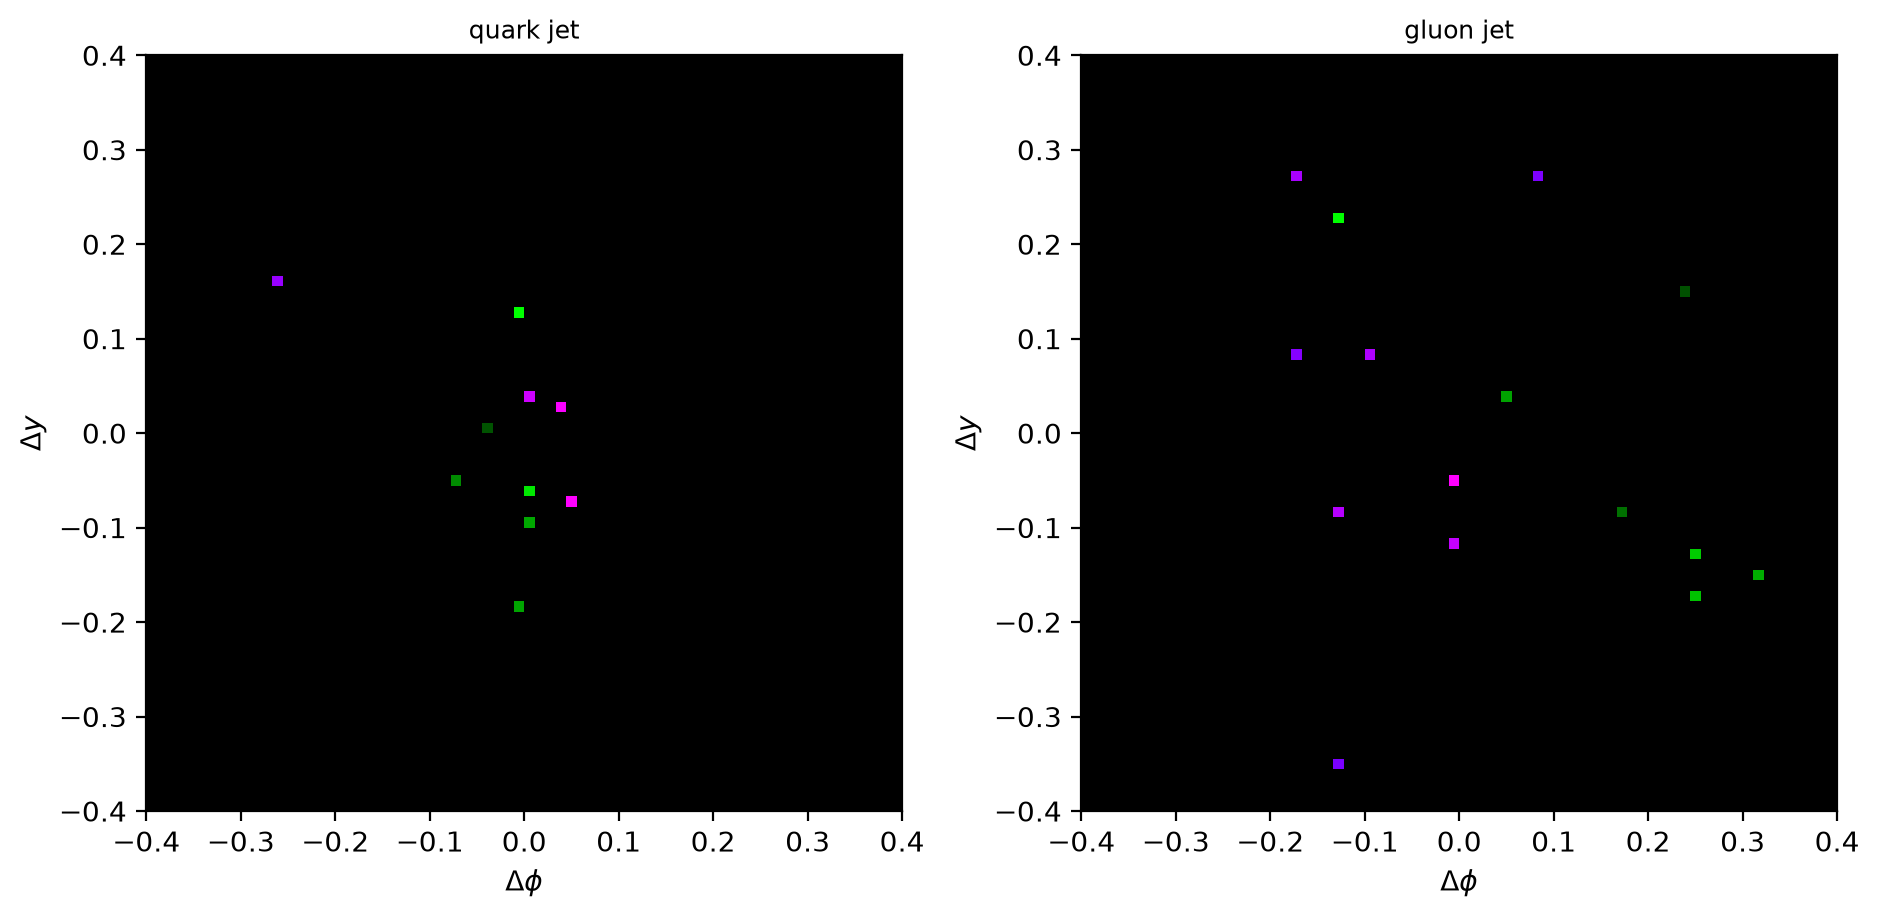
\includegraphics[width=\linewidth]{figures/qgjet_images}
	\caption{Jet images of a typical quark (left) and gluon (right) jet in \(\Delta y\) and \(\Delta\phi\) around the jet axis, with the image channels defined in the text. Gluon jets exhibit a broader spatial radiation pattern
		and higher particle multiplicity compared to quark jets}
	\label{fig:qgJetExamples}
\end{figure}

The images were input for a Convolutional Neural Network (CNN) implemented using PyTorch as shown in fig.~\ref{fig:rgbnn}.  
%
Each convolutional layer consisted of 64 filters, with filter sizes of \(5\times5\), \(3\times3\), and \(3\times3\), respectively. The max-pooling layers performed a 2×2 down-sampling with a stride length of 2. The dense layer consisted of 128 units, with a dropout rate of 0.2 before and after it.
\begin{figure}
	\centering
	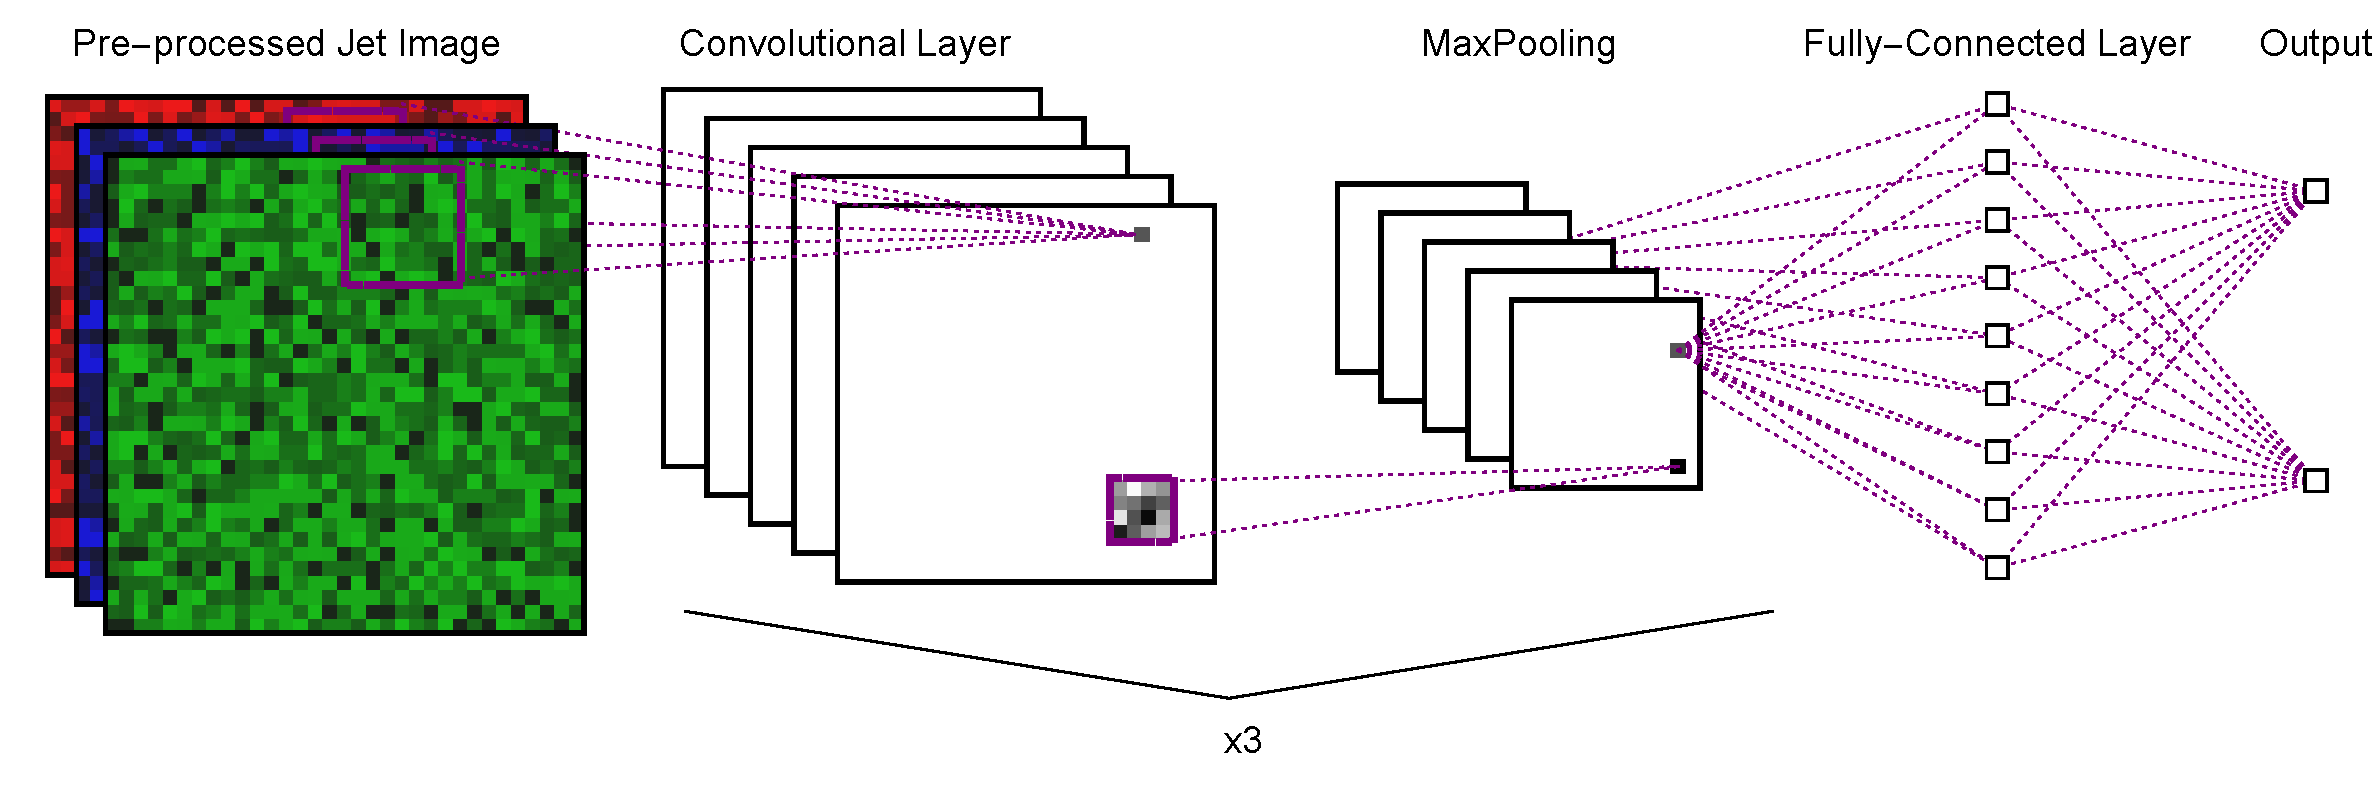
\includegraphics[width=1\linewidth]{figures/RGBNN}
	\caption{An illustration of the deep convolutional neural network architecture. The first
		layer is the input jet image, followed by three convolutional layers, a dense layer and an
		output layer.~\cite{Komiske_2017}}
	\label{fig:rgbnn}
\end{figure}

The network was trained with the AdamW optimizer at a learning rate of \(10^{-3}\) and a weight decay of 0.1, using the cross-entropy loss. 
%
Training used a batch size of 128 for 20 epochs, and the model with the lowest validation loss was retained. 
%
\begin{figure}
	\centering
	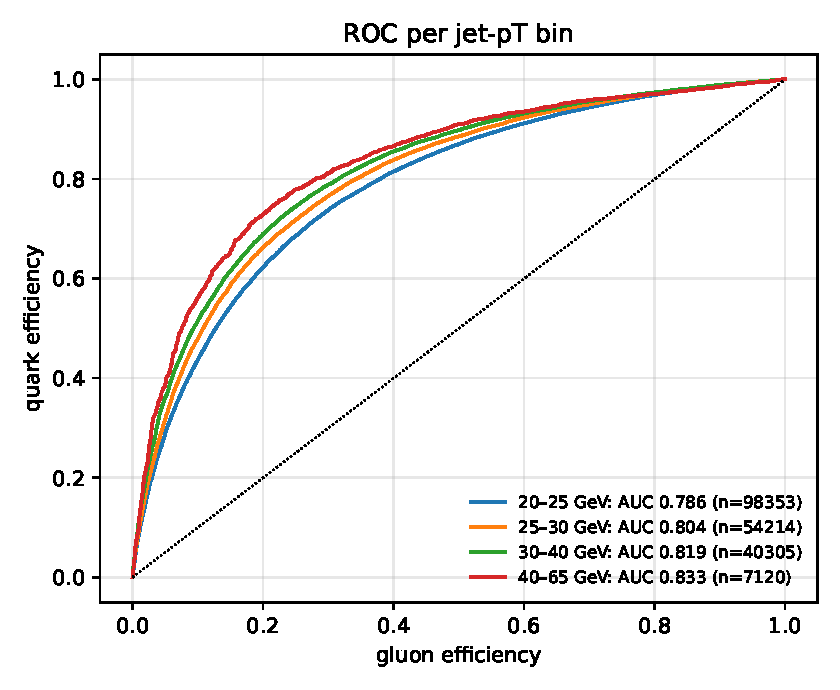
\includegraphics[width=0.7\linewidth]{figures/roc_per_jpt}
	\caption{ROC curves of the CNN quark-gluon classifier, quark efficiency vs gluon efficiency, evaluated on a holdout test set in bins of \(p_\mathrm{T, jet}\) (20--25, 25--30, 30--40 and 40--65 GeV/\(c\)). The area under the curve (AUC) rises from 0.79 to 0.83 with increasing \(p_\mathrm{T, jet}\). The diagonal corresponds to random guessing.}
	\label{fig:rocperjpt}
\end{figure}
Training images were augmented with random reflections in \(\Delta\eta\) and \(\Delta\phi\) and random translations of up to 0.5 pixels. 
%
The Receiver Operator Characteristic (ROC) curve, evaluated on a holdout test set, is shown differentially in \(p_\mathrm{T, jet}\) in Fig.~\ref{fig:rocperjpt}. The separation improves with \(p_\mathrm{T, jet}\), with the area under the curve increasing from 0.79 to 0.83. 


A way to gain some understanding of how the model looks at jet substructure is through \emph{interpretability} methods. 
%
We use a simple method of just noting the average change in classifier output upon masking a pixel. As seen in Fig.~\ref{fig:importancecnnqg}, the classifier relies mostly on the pixels close to the jet axis, and the region it uses becomes narrower for jets with higher \(p_\mathrm{T}\), which are more collimated.
\begin{figure}
	\centering
	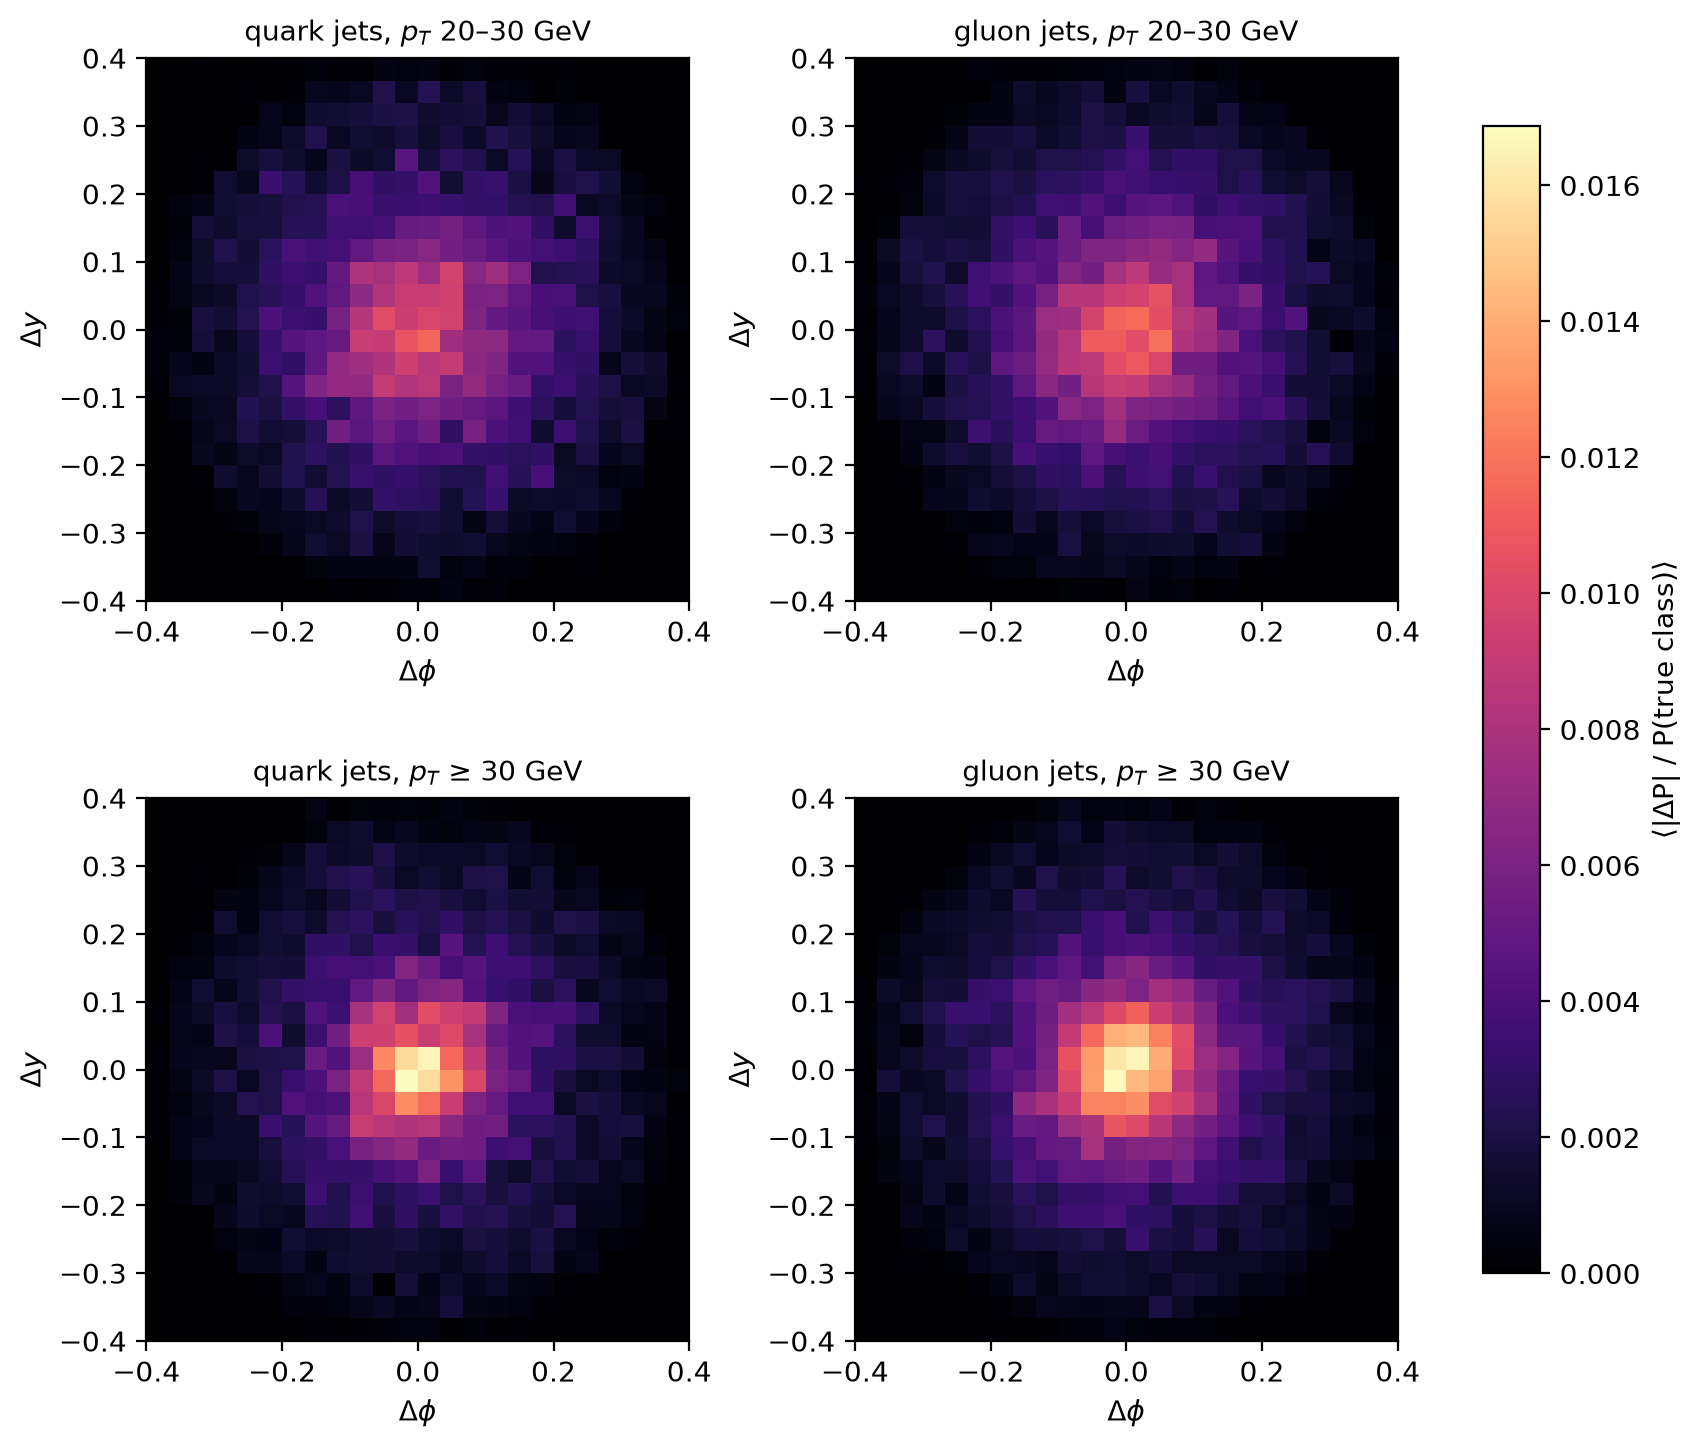
\includegraphics[width=0.7\linewidth]{figures/importance_cnn_qg}
	\caption{Per-pixel importance for the CNN quark-gluon classifier: the mean change of the classifier output when a pixel is masked, relative to the probability of the true class, \(\langle|\Delta P|\rangle/P(\text{true class})\), as a function of \(\Delta y\) and \(\Delta\phi\) from the jet axis, for quark (left) and gluon (right) jets with \(20 < p_\mathrm{T, jet} < 30\)~GeV/\(c\) (top) and \(p_\mathrm{T, jet} \geq 30\)~GeV/\(c\) (bottom).}
	\label{fig:importancecnnqg}
\end{figure}
\subsection{Characterizing jet quenching}
Another way to think about jet quenching/modification, is to ask how easily can a classifier algorithm tell apart the quenched and unquenched jet. 
%
Here we take PYTHIA-6~\cite{Sj_strand_2006} as the source of unquenched jets and JEWEL \cite{Zapp:2013vla} generates quenched jets in different centrality bins with/without recoil centers. 
%
Jets are represented as a 9-D vectors of features: $p_{\rm T, jet}$, $\rm N^{charged}_{\rm constit., jet}$, $\rm N^{neutral}_{\rm constit., jet}$, LeSub, $\lambda^2_0$, $\lambda_1^{0.5}$, $\lambda_1^1$, $\lambda_1^2$.
%
The jets are input into Dense Neural Networks (DNNs) with three hidden layers with 100 nodes each. After training, we calculate ROC curves shown in Fig.~\ref{fig:jetQuenchROC} using a holdout test set.
%
\begin{figure}
	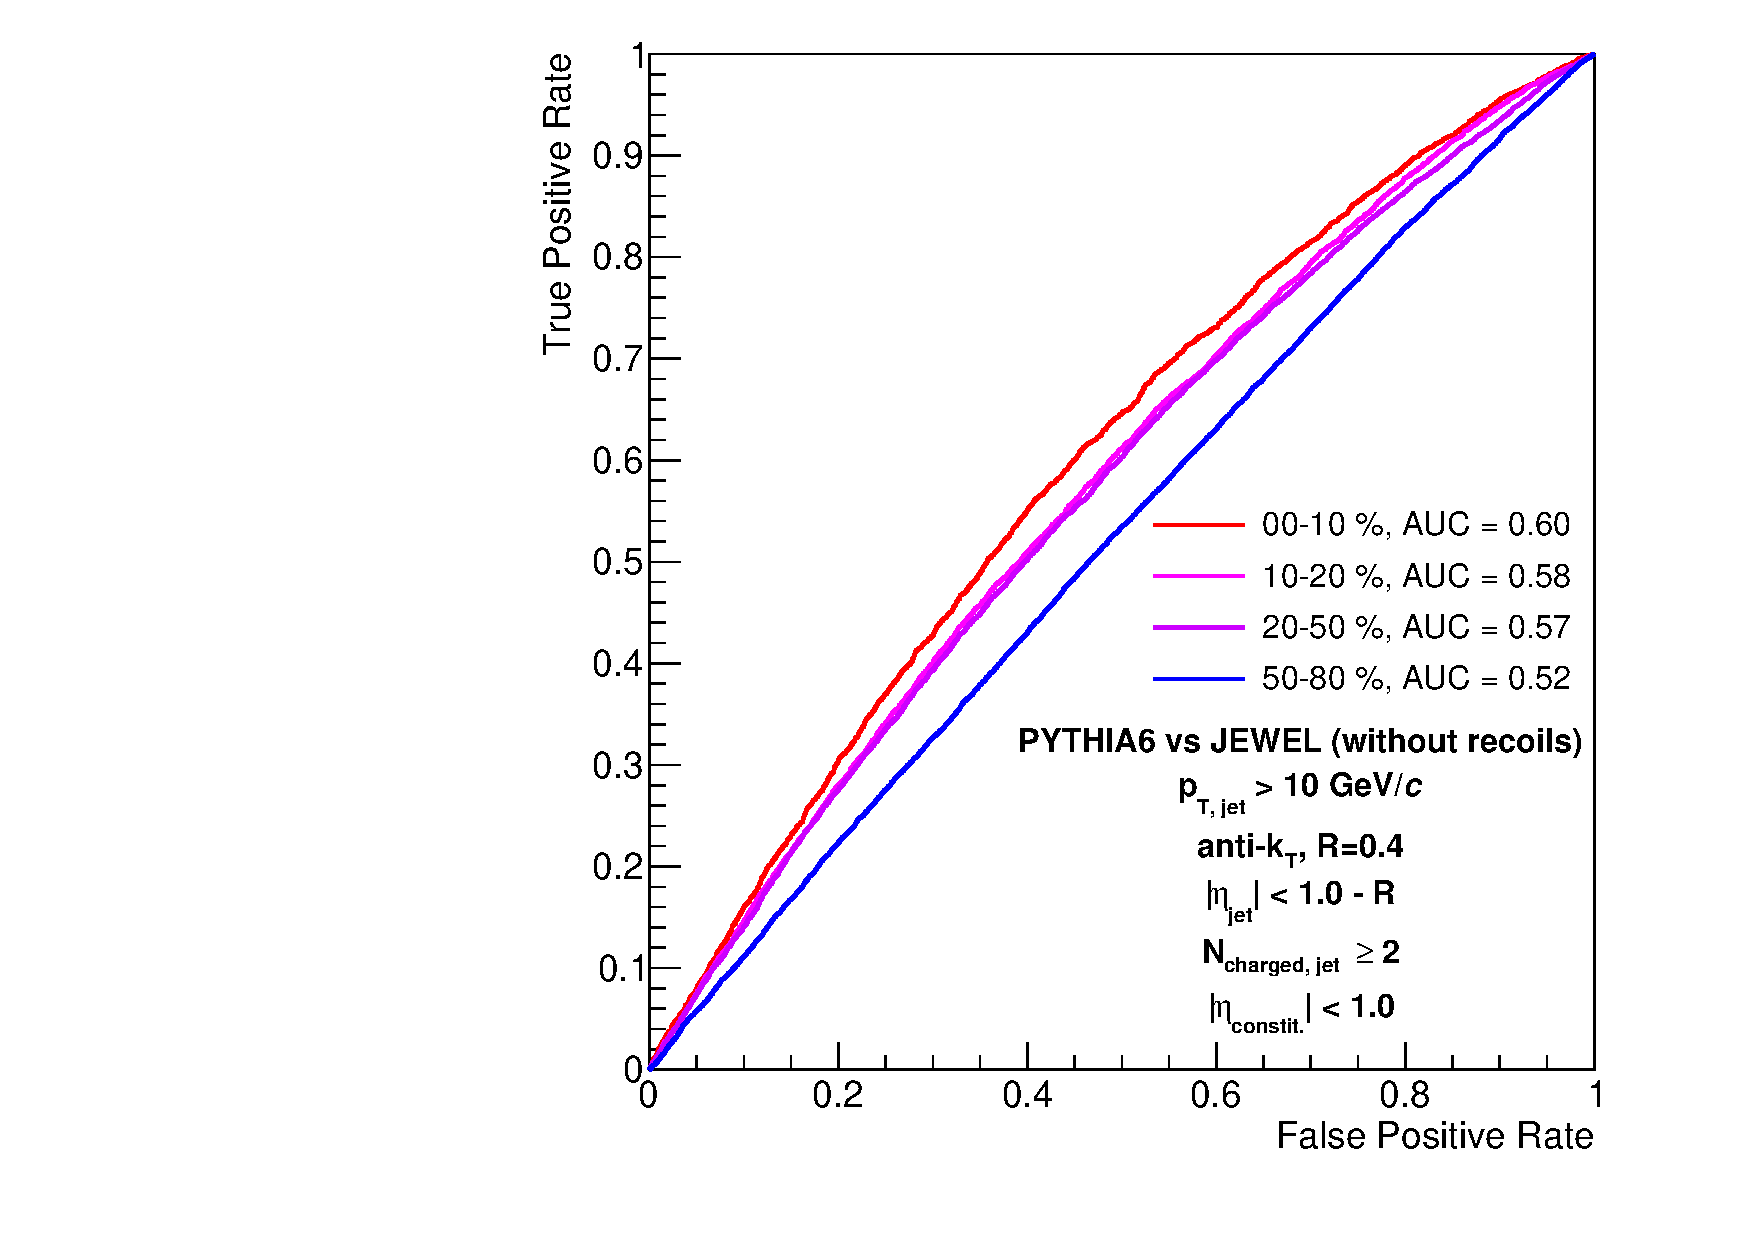
\includegraphics[width=0.49\linewidth]{roc_curve_dnn_withoutRec.pdf}
	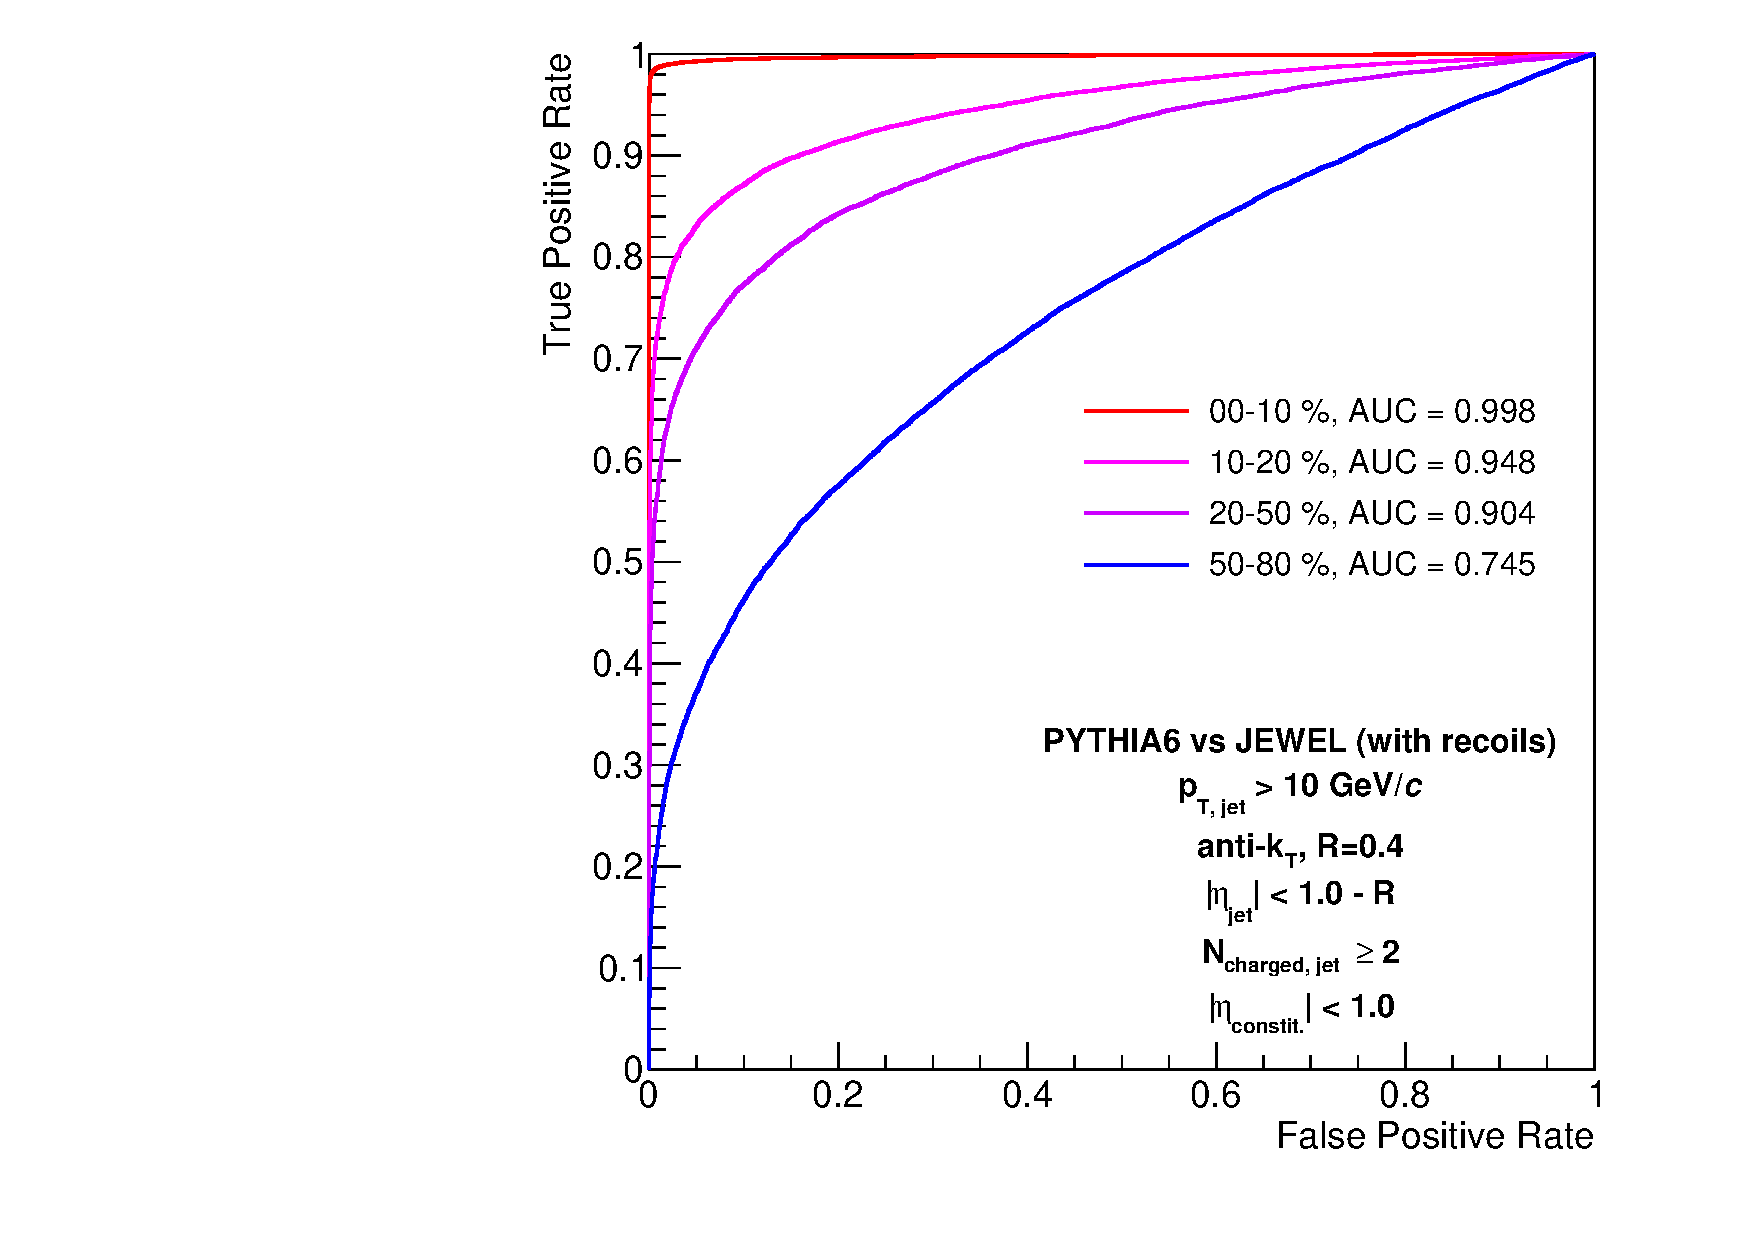
\includegraphics[width=0.49\linewidth]{roc_curve_dnn_wRec.pdf}
	\caption{ROC curves of the DNN classifier separating PYTHIA-6 (unquenched) from JEWEL (quenched) jets, for JEWEL without recoils (left) and with recoils (right), in four centrality classes, with the corresponding AUC values in the legends. Jets are anti-\(k_\mathrm{T}\), \(R = 0.4\), \(p_\mathrm{T, jet} > 10\)~GeV/\(c\), \(|\eta_\mathrm{jet}| < 1 - R\), with at least two charged constituents.}
	\label{fig:jetQuenchROC}
\end{figure}
%
The DNN performs better than chance in all the centralities and for both with/without recoils case.
The with-recoils case gives exagerrated ROC curves due to the background of recoil centers. 
%
AUC score decreases from central (0-10\%) to peripheral (50-80\%) events possibly implying more modification in central compared to peripheral.  
%
More information about jet quenching and machine learning can be found in~\cite{lai2022informationcontentjetquenching}

\chapter{Unfolding}
\label{app:Unfolding}

For any experiment, there is a disconnect between the desired phenomena (\emph{truth} level) and the measurement (\emph{measured} level) due to limitations of the detector setup. This is portrayed in Fig.~\ref{fig:UnfoldingScheme} through a dijet event at the truth level, whose final state charged and neutral particles are recorded as TPC tracks and BEMC towers.  Each of the detectors smear the energy and momenta and for almost all experiments,  the information about particle species is lost. For example, at STAR often a \(\pi^0\) mass assumption is taken for measured constituents. Thus jets, which are composite objects of these tracks and towers are non-trivially modified by a complicated convolution of these effects. Even with the best background removal procedure, jets will contain some residual background fluctuations from the underlying event.

\begin{figure}
	\centering
	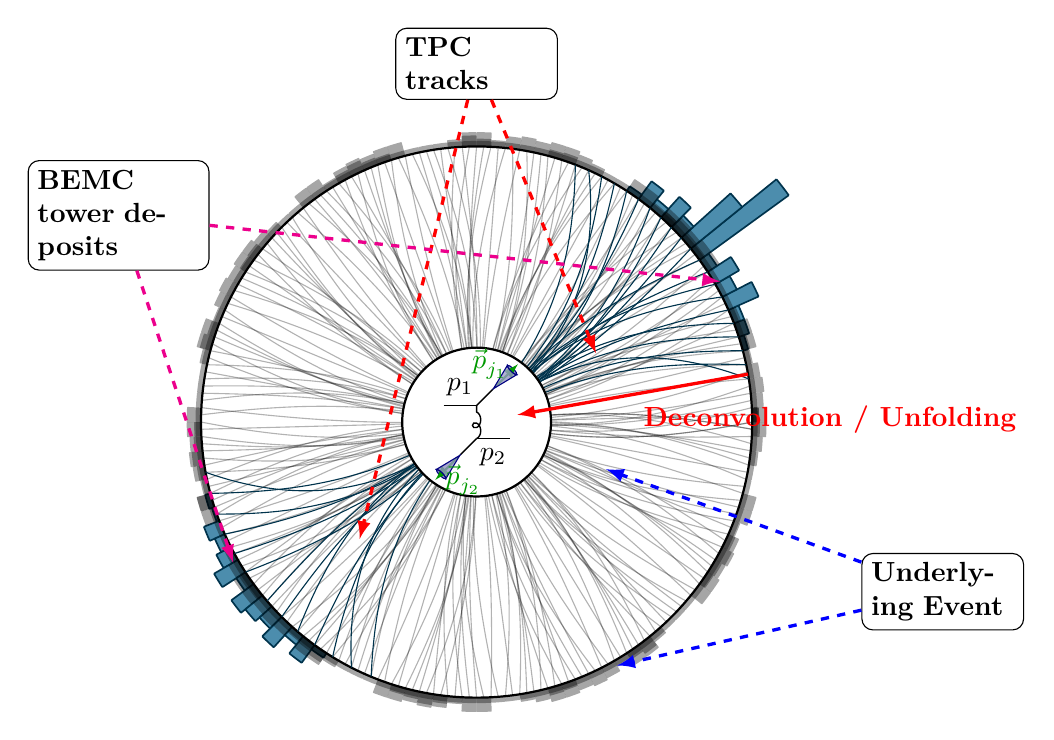
\begin{tikzpicture}[scale=0.7,rotate=0]
		\def\R{5} % tracker outer radius
		\def\dang{3} % angular granularity of calo deposits, 
		% HCAL DEPOSITS
		\foreach \dr [count=\i,
		evaluate={\r=\R+\dr; \anga=12+\dang*\i; \angb=\anga+\dang;}
		] in {0.1, 0.2, 0.2, 0.6, 0.3,0.5,0.2,2.0,1.2,0.3,0.5, 0.2, 0.4, 0.1}{
			\draw[calo] (0,0) -- (\anga:\r) arc(\anga:\angb:\r) -- cycle;
			%\draw[calo]
			%  (\anga:\R) -- (\anga:\r) arc(\anga:\angb:\r)
			%  -- (\angb:\R) arc(\angb:\anga:\R) -- cycle;
		}
		
		\foreach \dr [count=\i,
		evaluate={\r=\R+\dr; \anga=192+\dang*\i; \angb=\anga+\dang;}
		] in {0.1, 0.05, 0.3, 0.2,0.3,0.5,0.2, 0.5,0.4,0.3,0.5, 0.2, 0.4, 0.1}{
			\draw[calo] (0,0) -- (\anga:\r) arc(\anga:\angb:\r) -- cycle;
			%\draw[calo]
			%  (\anga:\R) -- (\anga:\r) arc(\anga:\angb:\r)
			%  -- (\angb:\R) arc(\angb:\anga:\R) -- cycle;
		}
		
		\foreach \ang [count=\i, 
		evaluate={\stepa = 15;
			\stepb=\stepa+50;
			\ra=\R+0.25*sin(\dang*\i*10); 
			\rb=\R+0.2*cos(\dang*\i*15);
			\rc=\R+0.3*sin(\dang*\i*20);
			\rd=\R+0.1;
		}]in {0, 3,...,360}{
			\draw[calobg] (0,0) -- (\ang:\ra) arc(\ang:\ang+\dang:\ra) -- cycle;
			\draw[calobg] (0,0) -- (\ang:\rd) arc(\ang:\ang+\dang:\rd) -- cycle;
			\draw[calobg] (0,0) -- (\stepa*\dang+\ang:\rb) arc(\stepa*\dang+\ang:\stepa*\dang+\ang+\dang:\rb) -- cycle;
			\draw[calobg] (0,0) -- (\stepb*\dang+\ang:\rc) arc(\stepb*\dang+\ang:\stepb*\dang+\ang+\dang:\rc) -- cycle;
		}
		
		\draw[thick,fill=white] (0,0) circle(\R); 
		
		\foreach \ang [count=\i,
		evaluate={\bend=12*sin(20+\i*\dang*15)}]in {0, 3,...,360}{
			\draw[black,opacity=0.3,thin,fill=none]
			(0,0) to[bend right=\bend] (\ang:\R);
		}
		
		\foreach \ang [count=\i,
		evaluate={\bend=12*cos(\i*\dang*15)}]in {0, 3,...,360}{
			\draw[black,opacity=0.3,thin,fill=none]
			(0,0) to[bend left=\bend] (\ang-\dang*0.5:\R);
		}
		
		%\draw[calo]
		%  (\anga:\R) -- (\anga:\r) arc(\anga:\angb:\r)
		%  -- (\angb:\R) arc(\angb:\anga:\R) -- cycle;
		
		\foreach \bend [count=\i,
		evaluate={\anga=6+\dang*\i;}
		] in {30, 14, 15,18, 20, 12, 19, 17, 11, 12}{
			\draw[blue!60!green!50!black,thin,fill=none]
			(0,0) to[bend left=\bend] (\anga:\R);	
		}	
		
		\foreach \bend [count=\i,
		evaluate={\anga=72-\dang*\i;}
		] in {20, 30, 19, 18, 20, 12, 19, 17, 12, 10, 8}{
			\draw[blue!60!green!50!black,thin,fill=none]
			(0,0) to[bend right=\bend] (\anga:\R);
		}
		
		\foreach \bend [count=\i,
		evaluate={\anga=186+1.5*\dang*\i;}
		] in {30, 14, 20, 12, 11, 12}{
			\draw[blue!60!green!50!black,thin,fill=none]
			(0,0) to[bend left=\bend] (\anga:\R);
		}
		
		\foreach \bend [count=\i,
		evaluate={\anga=252-1.5*\dang*\i;}
		] in {20, 30, 19, 12, 19, 10, 8}{
			\draw[blue!60!green!50!black,thin,fill=none]
			(0,0) to[bend right=\bend] (\anga:\R);
		}
		
		\node[draw, text width=0.15\textwidth, rounded corners=4pt] (tracks) at (90:1.3*\R){
			\textbf{TPC tracks}
		};		
		\draw (tracks) edge[dashed,  ->, very thick, red] (225:0.6*\R);
		\draw (tracks) edge[dashed,  ->, very thick, red] (30:0.5*\R);
		
		\node[draw, text width=0.17\textwidth, rounded corners=4pt] (towers) at (150:1.5*\R){
			\textbf{BEMC tower deposits} 
		};		
		\draw (towers) edge[dashed,  ->, very thick, magenta] (210:1.02*\R);
		\draw (towers) edge[dashed,  ->, very thick, magenta] (30:1.02*\R);
		
		\node[draw, text width=0.15\textwidth, rounded corners=4pt] (UE) at (340:1.8*\R){
			\textbf{Underlying Event}
		};		
		\draw (UE) edge[dashed, ->, very thick, blue] (300:1.02*\R);
		\draw (UE) edge[dashed,  ->, very thick, blue] (340:0.5*\R);
		
		\draw[thick,fill=white] (0,0) circle(0.27*\R); 
		\begin{feynhand}[scale=0.3]
			\vertex (a)  at (-1, -2); 
			\vertex(b)  at (-2, 1); 
			\vertex (c)  at (0, -1); 
			\vertex (d)  at (0, 1);
			\propag [plain] (c) to (a);
			\propag [plain] (b) to  [edge label = $p_1$] (d);
			\propag [gluon] (c) to (d);
			\vertex(e) at (2, -1) ; 
			\vertex (f) at (1, 2);
			\propag [plain] (e) to [edge label = $p_2$](c);
			\propag [plain] (d) to (f);
			\coordinate (J1) at (2.5,3.5);
			\coordinate (J2) at (-2.5, -3.5);
			\jetcone{f}{J1}{0.4}{0.10}
			\jetcone{a}{J2}{0.4}{0.10}
			\node[vector,left] at (J1) {$\vv{p}_{j_1}$};
			\node[vector,right] at (J2) {$\vv{p}_{j_2}$};
		\end{feynhand}		
		
		\draw  (10:\R) edge["\textbf{Deconvolution / Unfolding}", ->, very thick, red] (10:0.15*\R);
	\end{tikzpicture}
	\caption[Schematic of the unfolding of detector effects]{Schematic figure showing the unfolding procedure. The desired physics / truth / particle level is represented by the \(2\to 2\) Feynman diagram in the middle. The blue (gray) tracks and tower deposits are the dijet (underlying) event as recorded by the TPC and BEMC. }
	\label{fig:UnfoldingScheme} 
\end{figure}

Thus distributions of any jet observable \(\mathbf{O}\) will have these \emph{detector effects} which will need to be removed in order for the measurement to be comparable to theory calculations. In other terms, a truth value of \(\mathbf{x}\) can manifest as a range of measured values \((\mathbf{x}_0, \mathbf{x}_1)\) similarly, a measured value of \(\mathbf{y}\) can come from a range of truth values \((\mathbf{y}_0, \mathbf{y}_1)\).  Thus, using Bayes theorem, the probability either measured value being  \(\mathbf{y}\)  or truth value being  \(\mathbf{x}\) would be,

\begin{align}
	\label{eq:trMeas}
	p_\mathrm{meas.}(\mathbf{y}) &= \int d\mathbf{x}~p_\mathrm{meas.|tr.}(\mathbf{y} |  \mathbf{x}) p_\mathrm{tr.}(\mathbf{x}) \notag\\
	p_\mathrm{tr.}(\mathbf{x}) &= \int d\mathbf{y}~p_\mathrm{tr.|meas.}(\mathbf{x} |  \mathbf{y}) p_\mathrm{meas.}(\mathbf{y}).
\end{align}



From Eq.~\ref{eq:trMeas}, we measure \(p_\mathrm{meas.}\) through histograms, density estimates, etc. and \(p_\mathrm{tr.}\) is what we want to determine. Now, \(p_\mathrm{meas.|tr.}\) represents the detector's \emph{response}, which can be obtained to a high degree of accuracy from simulation programs like GEANT~\cite{MISC-15}. We can start from a \emph{generated} truth distribution  \(p_\mathrm{gen., 0}\) and obtain the \emph{reconstructed} measured distribution  \(p_\mathrm{reco., 0}\). Thus the assumption is, 
\begin{align}
	\label{eq:responseTransfer}
	p_\mathrm{meas.|tr.}(\mathbf{y} |  \mathbf{x}) = p_\mathrm{reco.|gen., 0}(\mathbf{y} |  \mathbf{x}) \equiv R(\mathbf{y}, \mathbf{x}) ,
\end{align}
Substituting \(R(\mathbf{y}, \mathbf{x})\) in Eq.~\ref{eq:trMeas} and using \(\omega_0(\mathbf{y}) = p_\mathrm{meas.}(\mathbf{y})/p_\mathrm{reco., 0}(\mathbf{y})\)
\begin{align}
	\label{eq:unfoldEstimator}
	p_\mathrm{gen., 1}(\mathbf{x}) &\equiv \int d\mathbf{y}~p_\mathrm{gen.|reco., 0}(\mathbf{x} |  \mathbf{y})\,p_\mathrm{meas.}(\mathbf{y}) \notag\\
	&=\int d\mathbf{y}~\frac{R(\mathbf{y}, \mathbf{x})\,p_\mathrm{gen., 0}(\mathbf{x})}{p_\mathrm{reco., 0}(\mathbf{y})} p_\mathrm{meas.}(\mathbf{y})\notag\\
	&= p_\mathrm{gen., 0}(\mathbf{x})\int d\mathbf{y}~R(\mathbf{y}, \mathbf{x})\,\omega_0(\mathbf{y}).
\end{align}
Using \(\nu_0(\mathbf{x}) = p_\mathrm{gen., 1}(\mathbf{x})/p_\mathrm{gen., 0}(\mathbf{x})\) measured distribution correspondingly becomes,
\begin{align}
	\label{eq:step2Joint}
	p_\mathrm{reco., 1}(\mathbf{y}) &= \int d\mathbf{x}~(\mathbf{x})\,R(\mathbf{y}, \mathbf{x})\,p_\mathrm{gen., 1}(\mathbf{x})\notag\\
	&= p_\mathrm{reco., 0}(\mathbf{y}) \int d\mathbf{x}~\frac{R(\mathbf{y}, \mathbf{x})\,p_\mathrm{gen., 0}(\mathbf{x})}{p_\mathrm{reco., 0}(\mathbf{y})}\nu_0(\mathbf{x}). 
\end{align}
The convolutions \(\int d\mathbf{y}~R(\mathbf{y}, \mathbf{x})\,\omega_0(\mathbf{y})\) and \(\int d\mathbf{x}~R(\mathbf{y}, \mathbf{x})\frac{\,p_\mathrm{gen., 0}(\mathbf{x})}{p_\mathrm{reco., 0}(\mathbf{y})}\nu_0(\mathbf{x})\) are mapping \(\omega_0(\mathbf{y})\to\omega_0(\mathbf{x})\) and \(\nu_0(\mathbf{x})\to\nu_0(\mathbf{y})\) respectively. 
%
For the \(n^\text{th}\) iteration, 
%
\begin{align}
	\label{eq:generalUnfolding}
	\omega_{n-1}(\mathbf{y}) &= \frac{p_\mathrm{meas.}(\mathbf{y})}{p_{\mathrm{reco.}, n-1}(\mathbf{y})} \notag\\
	p_{\mathrm{gen.}, n}(\mathbf{x}) &= p_{\mathrm{gen.}, n-1}(\mathbf{x})\int d\mathbf{y}~R(\mathbf{y}, \mathbf{x})\,\omega_{n-1}(\mathbf{y})\notag\\
	\nu_{n-1}(\mathbf{x}) &= \frac{p_{\mathrm{gen.}, n}(\mathbf{x})}{p_{\mathrm{gen.}, n-1}(\mathbf{x})} \notag\\
	p_{\mathrm{reco.}, n}(\mathbf{y}) &= p_{\mathrm{reco.}, n-1}(\mathbf{y}) \int d\mathbf{x}~R(\mathbf{y}, \mathbf{x})\frac{p_{\mathrm{gen.}, n-1}(\mathbf{x})}{p_{\mathrm{reco.}, n-1}(\mathbf{y})}\nu_{n-1}(\mathbf{x}). 
\end{align}
%
Given convergence, \(p_{\mathrm{reco.}, n}(\mathbf{y}) \to p_\mathrm{gen.}(\mathbf{y})\) and \(p_{\mathrm{tr.}, n}(\mathbf{x}) \to p_{\mathrm{unf.}}(\mathbf{x})\) is the unfolded distribution. 

%Generated jets without a reconstructed partner (\emph{misses}, \(\mathbf{y}=\varnothing\)) carry no \(\omega_{n-1}\), and reconstructed jets without a generated partner (\emph{fakes}, \(\mathbf{x}=\varnothing\)) carry no \(\nu_{n-1}\). Each receives its missing weight from the corresponding map of Eq.~\ref{eq:generalUnfolding}, built from matched pairs and normalized over them,
%\begin{align}
%	\label{eq:missFakeWeights}
%	\omega_{n-1}(\mathbf{x}) &= \frac{\int d\mathbf{y}~R(\mathbf{y}, \mathbf{x})\,\omega_{n-1}(\mathbf{y})}{\int d\mathbf{y}~R(\mathbf{y}, \mathbf{x})}
%	= \frac{\int d\mathbf{y}~R(\mathbf{y}, \mathbf{x})\,\omega_{n-1}(\mathbf{y})}{\epsilon(\mathbf{x})} ,
%	&&\mathbf{y}=\varnothing , \notag\\
%	\nu_{n-1}(\mathbf{y}) &= \frac{\int d\mathbf{x}~R(\mathbf{y}, \mathbf{x})\,p_{\mathrm{gen.}, n-1}(\mathbf{x})\,\nu_{n-1}(\mathbf{x})}{\int d\mathbf{x}~R(\mathbf{y}, \mathbf{x})\,p_{\mathrm{gen.}, n-1}(\mathbf{x})} ,
%	&&\mathbf{x}=\varnothing ,
%\end{align}
%where \(\epsilon(\mathbf{x})\) is the reconstruction efficiency and the second denominator is \(p_{\mathrm{reco.}, n-1}(\mathbf{y})\) of matched jets. A miss at \(\mathbf{x}\) thus enters the second step with the mean first-step weight of the matched generated jets at \(\mathbf{x}\), and a fake at \(\mathbf{y}\) enters the next iteration with the weight the matched reconstructed jets at \(\mathbf{y}\) acquire from \(\nu_{n-1}\). Eq.~\ref{eq:generalUnfolding} then holds on the full samples,
%\begin{align}
%	\label{eq:missFakeIteration}
%	p_{\mathrm{gen.}, n}(\mathbf{x}) &= \omega_{n-1}(\mathbf{x})\,p_{\mathrm{gen.}, n-1}(\mathbf{x}) = \nu_{n-1}(\mathbf{x})\,p_{\mathrm{gen.}, n-1}(\mathbf{x}) , &&\text{matched and missed,} \notag\\
%	p_{\mathrm{reco.}, n}(\mathbf{y}) &= \nu_{n-1}(\mathbf{y})\,p_{\mathrm{reco.}, n-1}(\mathbf{y}) , &&\text{matched and fake,}
%\end{align}
%so that \(\nu_{n-1}\) is formed over a generated distribution that includes misses, and \(\omega_n\) against a reconstructed distribution that includes fakes.

This algorithm can be adapted for binned data by expressing the distributions as vectors representing bin counts of histograms and \(R(\mathbf{y}, \mathbf{x})\) as a matrix, giving the traditional method of \emph{Iterative Bayesian Unfolding}~\cite{bennerRoounfold}. Although it has been the standard for a long time, the required binning of data limits its usefulness beyond 3-dimensions. Also, not all measurements can be straightforwardly represented in the response matrix. 

\begin{figure}
	\centering
	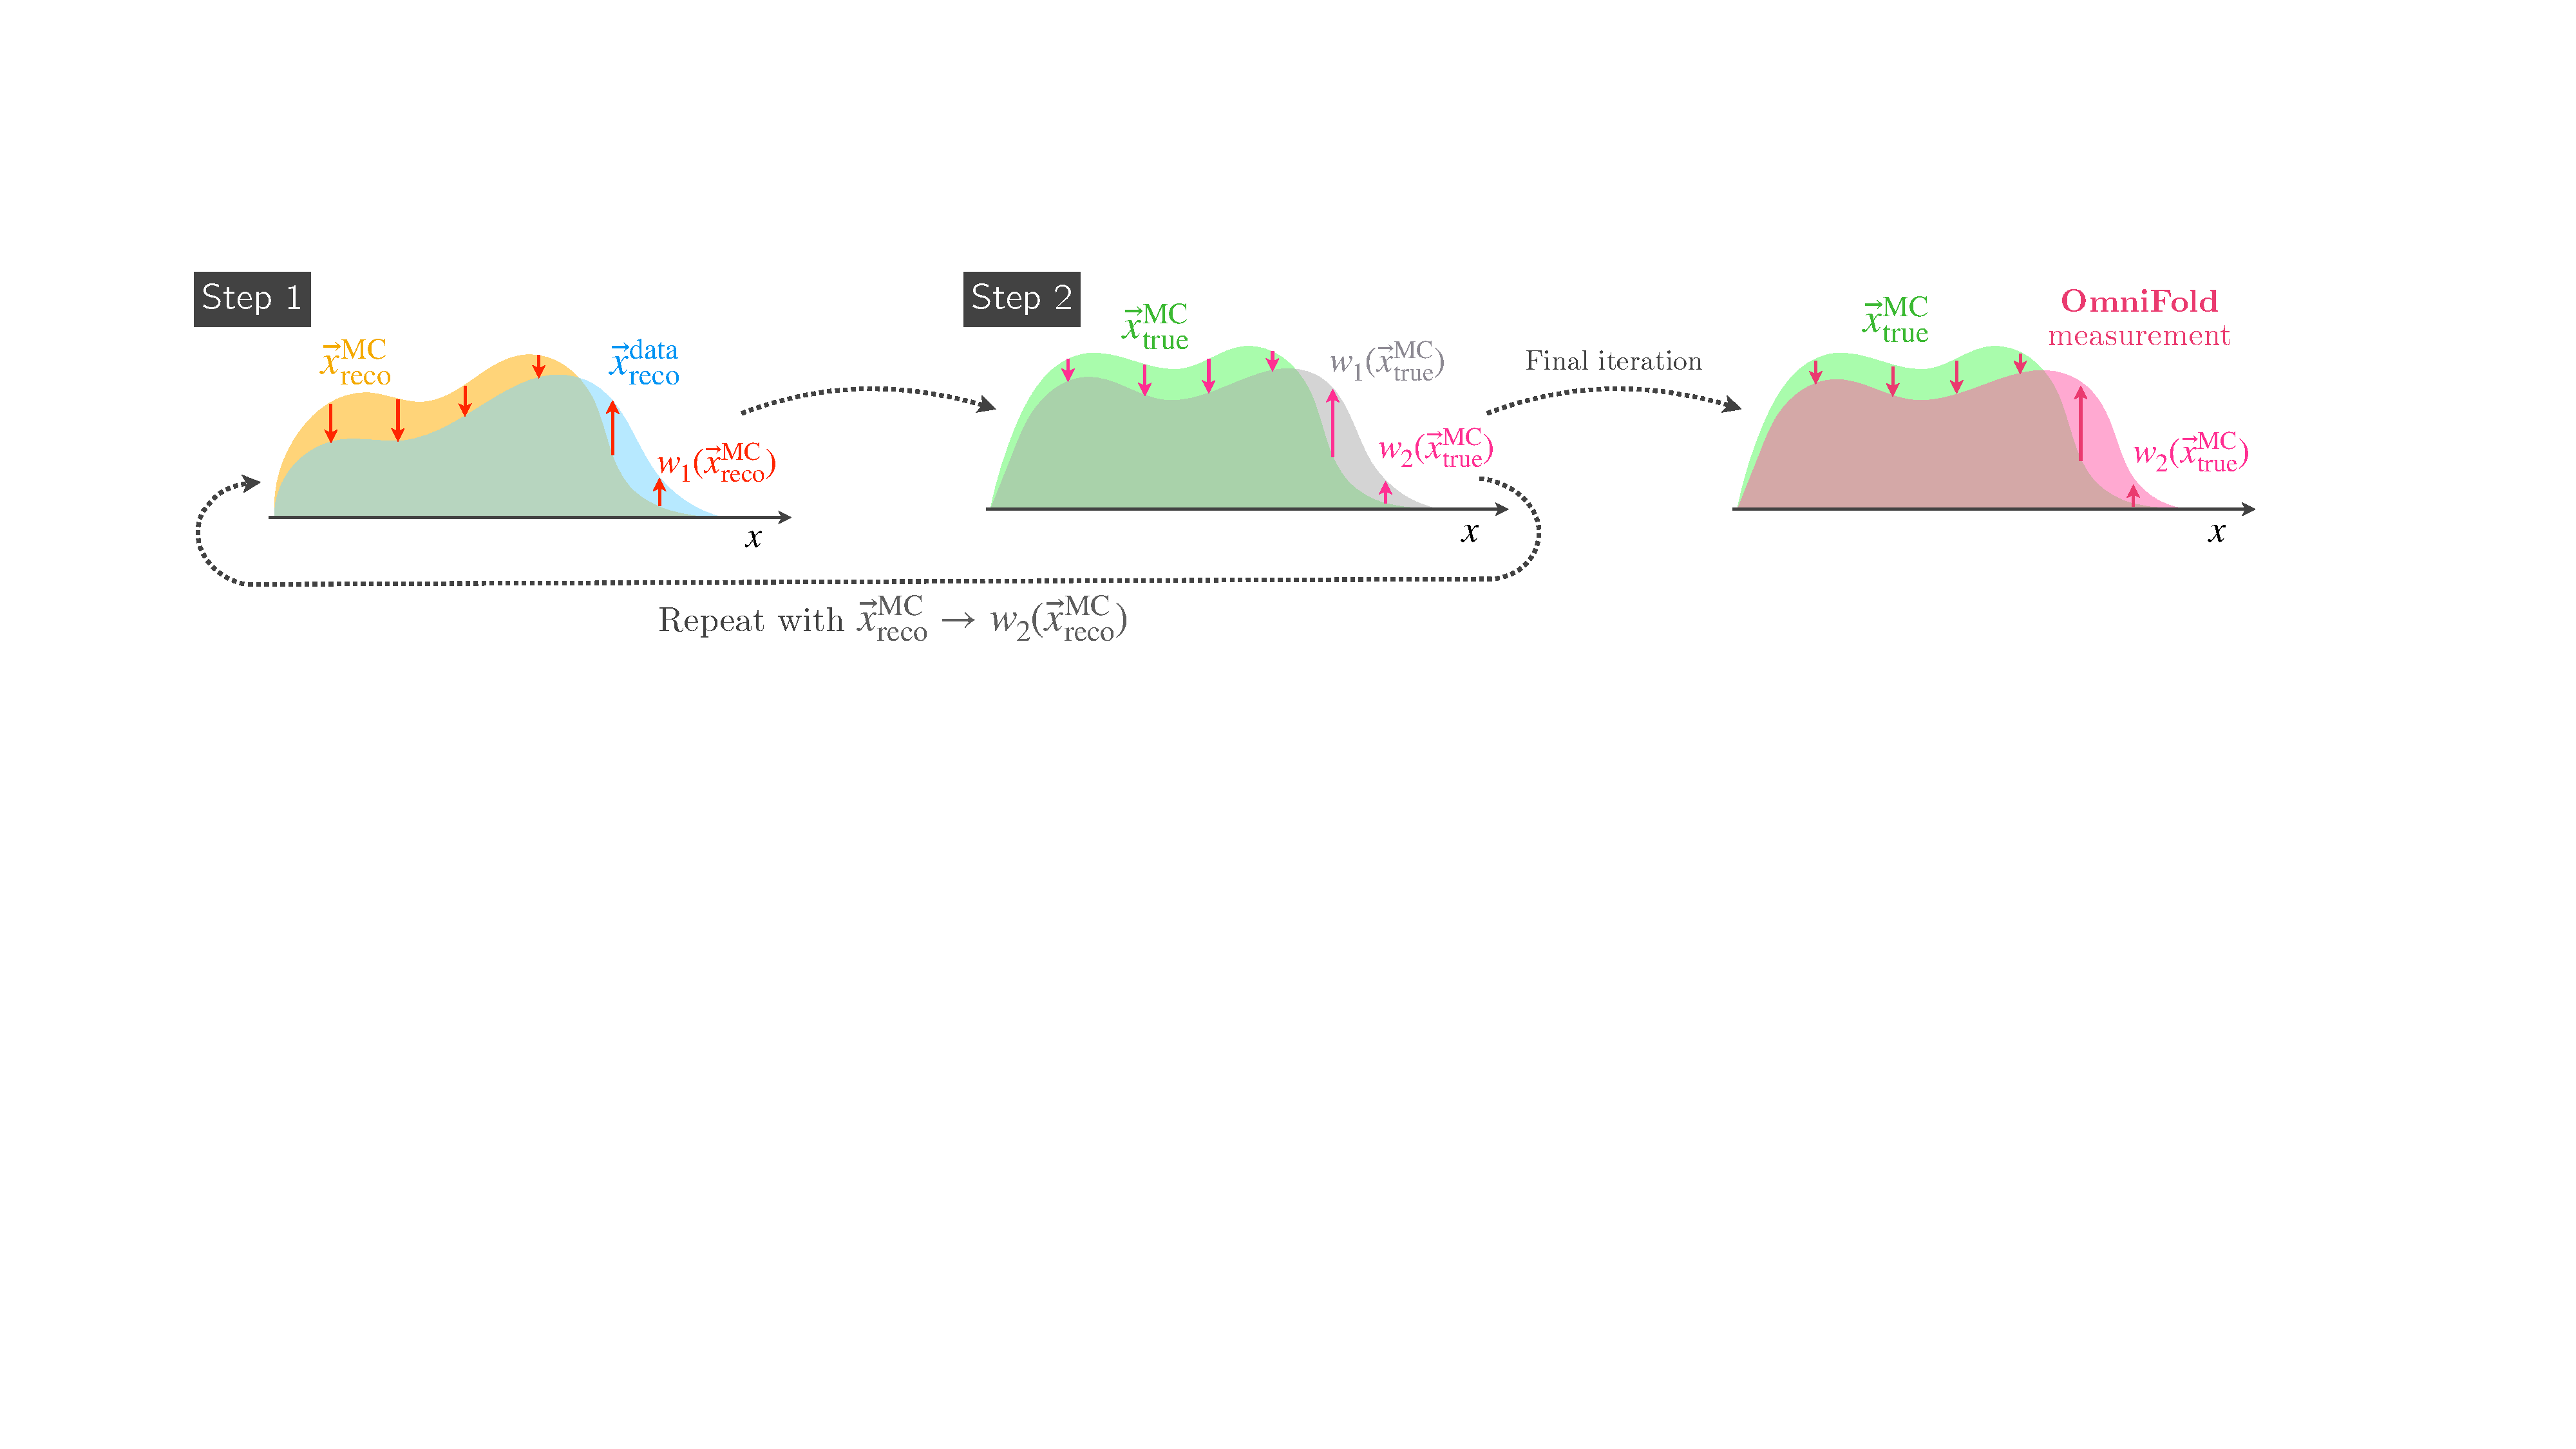
\includegraphics[width=1\linewidth]{figures/omnifold_fig_2025_04_24}
	\caption[Illustration of the OmniFold method]{Illustration of the OmniFold method. In Step 1, MC is corrected to match data at the detector level, producing a weighting function $w_1(\vec{x}_{\text{reco}}^{\text{ MC}})$. In Step 2, a new function $w_2(\vec{x}_{\text{true}}^{\text{ MC}})$ is learned based only on particle-level quantities. The method proceeds iteratively, refining the function $w_2(\vec{x}_{\text{true}}^{\text{ MC}})$ such that the particle-level MC can be reweighted to give event yields and kinematics that match those observed in the data~\cite{Canelli_2026}.}
	\label{fig:omnifold}
\end{figure}

One of the first unbinned approaches, OmniFold~\cite{PhysRevLett.124.182001} (Fig.~\ref{fig:omnifold}), uses classifiers to calculate the ratios \(\omega\) and \(\nu\). For \(i^\text{th}\) iteration, \(\omega_{i-1}(\mathbf{y})\) can be calculated using classifier \(f_\mathrm{meas., reco}\) which classifies a jet represented by \(\mathbf{y}\) as measured or reconstructed. Thus, 
\begin{equation}
	\omega_{i-1}(\mathbf{y}) = \frac{f_\mathrm{meas., reco}(\mathbf{y})}{1 - f_\mathrm{meas., reco}(\mathbf{y})}
\end{equation}
and \(\nu_{i-1}(\mathbf{y})\) can be calculated using classifier \(f_{i, i-1}\) which classifies a jet represented by \(\mathbf{x}\) as being generated from \(i^\text{th}\) or \((i-1)^\text{th}\) iteration. 
\begin{equation}
	\nu_{i-1}(\mathbf{x}) = \frac{f_{i, i-1}(\mathbf{x})}{1-f_{i, i-1}(\mathbf{x})}.
\end{equation}
Not every jet has a partner at the other level.
%
A generated jet whose reconstructed partner is lost, through the detector inefficiency, the resolution moving it out of the selection or a failed matching, is a \emph{miss}; a reconstructed jet without a generated partner, e.g.\ one formed from background fluctuations or moved into the selection by the resolution, is a \emph{fake}.
%
Misses have no \(\mathbf{y}\) and therefore no \(\omega_{i-1}(\mathbf{y})\), and fakes have no \(\mathbf{x}\) and therefore no \(\nu_{i-1}(\mathbf{x})\), so each needs its own estimate.
%
For misses, a classifier \(f^\mathrm{gen.}_{i, i-1}\) separates matched generated jets weighted by \(\omega_{i-1}(\mathbf{y})\) from those of the \((i-1)^\text{th}\) iteration; for fakes, a classifier \(f^\mathrm{reco.}_{i, i-1}\) separates matched reconstructed jets weighted by \(\nu_{i-1}(\mathbf{x})\) from those of the \((i-1)^\text{th}\) iteration,
\begin{equation}
	\omega_{i-1}(\mathbf{x}) = \frac{f^\mathrm{gen.}_{i, i-1}(\mathbf{x})}{1-f^\mathrm{gen.}_{i, i-1}(\mathbf{x})} ,
	\qquad
	\nu_{i-1}(\mathbf{y}) = \frac{f^\mathrm{reco.}_{i, i-1}(\mathbf{y})}{1-f^\mathrm{reco.}_{i, i-1}(\mathbf{y})} ,
\end{equation}
evaluated at the miss's \(\mathbf{x}\) and the fake's \(\mathbf{y}\) respectively. Thus, it takes 2-4 classifier trainings per unfolding iteration~\cite{andreassen2021scaffoldingsimulationsdeeplearning}.

The result of the unfolding is not a set of histograms but a weight for every generated jet.
%
Since each generated jet carries all the features \(\mathbf{x}\) it was unfolded with, any observable that is a function of \(\mathbf{x}\) can be computed from the weighted jets after the unfolding, in any binning, without repeating the unfolding: new observables can be studied with the same unfolded jets, as long as they are combinations of the unfolded features~\cite{PhysRevLett.124.182001,Canelli_2026}.
%
Observables that depend on information not contained in \(\mathbf{x}\) still require a new unfolding that includes it.

\chapter{Vectorized training of model ensembles}
\label{app:torchstrap}

The statistical uncertainties of the unbinned unfolding in Ch.~\ref{ch:angularities} are obtained by replacing every classifier of MultiFold with an ensemble of independently trained replicas (Sec.~\ref{sec:bootstrap}).
%
This is the bootstrap idea~\cite{Efron:1979bootstrap} applied to neural networks, where an ensemble of networks trained on resampled data also gives a well-calibrated estimate of the uncertainty of their prediction~\cite{Lakshminarayanan:2016ensembles}.
%
A MultiFold unfolding trains four classifiers per iteration, and it is repeated for every systematic variation, so an ensemble of \(N\) replicas multiplies an already long chain of trainings by \(N\).
%
This appendix describes \emph{torchstrap}\footnote{\url{https://github.com/TanmayPani/torchstrap}}, a PyTorch~\cite{Paszke:2019pytorch} library written for this thesis that trains all \(N\) replicas of an ensemble at once on a single GPU, as one vectorized computation rather than a loop over models.

\section{The cost of training replicas one by one}
\label{sec:tsMotivation}
The classifiers used here are small multi-layer perceptrons (MLPs), with a few hundred thousand parameters, trained on mini-batches of a few thousand jets.
%
Every operation of their training step, a matrix multiplication, an activation or an optimizer update, is a separate \emph{kernel} launched on the GPU, and a kernel acting on such small tensors finishes in a time comparable to the overhead of launching it.
%
Training \(N\) replicas one after the other, or in \(N\) separate processes, therefore multiplies the number of launches by \(N\) while leaving the GPU mostly idle, and separate processes in addition duplicate the memory of the framework itself.

The replicas, however, share their architecture and differ only in the values of their parameters and in the data they see.
%
For a dense layer with weights \(\Lambda^a_{\ b}\), acting on an input \(x_a\) as \(y_b = \Lambda^a_{\ b}\,x_a\), the \(N\) replicas
\begin{equation}
	y^{k}_{b} = \Lambda^{a,k}_{\ b}\,x^{k}_{a}, \qquad 1 \leq k \leq N,
	\label{eq:batchedLayer}
\end{equation}
are a single \emph{batched} matrix multiplication over the extra index \(k\), which runs as one kernel instead of \(N\).
%
Rewriting a whole model in this form by hand is error prone, but PyTorch provides the transformation \texttt{torch.func.vmap}, which turns a function written for one replica into one that acts on tensors with an additional leading replica dimension, adding the index \(k\) of Eq.~\ref{eq:batchedLayer} to every operation.
%
Fig.~\ref{fig:tsEnsembles} shows the three configurations discussed in this appendix: a single model, an ensemble of replicas trained on the same data, and a bootstrap ensemble in which every replica is trained on its own resample.

% ---------------------------------------------------------------------------
% Drawing helpers for this appendix
\tikzset{
	tsnode/.style={circle, draw=#1!60!black, fill=#1!25, thick, minimum size=4.2mm, inner sep=0pt},
	tsnode/.default=blue,
	tsedge/.style={draw=blue!30!black!40, line width=0.35pt},
	tscard/.style={draw=black!55, rounded corners=3pt, fill=white, line width=0.5pt},
	tscell/.style={draw=black!50, fill=#1, minimum width=9mm, minimum height=4.5mm, inner sep=0pt, font=\scriptsize},
	tscell/.default=blue!12,
	tsarrow/.style={-{Latex[length=2.2mm]}, thick, red!70!black},
}
% \tsMLP{x}{y}: a 2-4-4-1 MLP inside a card, lower-left corner of the card at (x,y)
\newcommand{\tsMLP}[2]{%
	\begin{scope}[shift={(#1,#2)}]
		\draw[tscard] (0,0) rectangle (3.3,2.0);
		\foreach \i in {1,2} \coordinate (in\i) at (0.35, {1.0+0.45*(\i-1.5)});
		\foreach \i in {1,...,4} \coordinate (ha\i) at (1.25, {1.0+0.42*(\i-2.5)});
		\foreach \i in {1,...,4} \coordinate (hb\i) at (2.15, {1.0+0.42*(\i-2.5)});
		\coordinate (out) at (2.95, 1.0);
		\foreach \i in {1,2} \foreach \j in {1,...,4} \draw[tsedge] (in\i) -- (ha\j);
		\foreach \i in {1,...,4} \foreach \j in {1,...,4} \draw[tsedge] (ha\i) -- (hb\j);
		\foreach \i in {1,...,4} \draw[tsedge] (hb\i) -- (out);
		\foreach \i in {1,2} \node[tsnode=green] at (in\i) {};
		\foreach \i in {1,...,4} \node[tsnode] at (ha\i) {};
		\foreach \i in {1,...,4} \node[tsnode] at (hb\i) {};
		\node[tsnode=red] at (out) {};
	\end{scope}}
% \tsCard{x}{y}: an empty card of the same size, for replicas behind the front one
\newcommand{\tsCard}[2]{\draw[tscard] (#1,#2) rectangle ++(3.3,2.0);}
% \tsData{x}{y}{label of sample i}{fill}: a 2 x 4 block of (x, y) inputs, lower-left corner at (x,y)
\newcommand{\tsData}[4]{%
	\begin{scope}[shift={(#1,#2)}]
		\foreach \c/\s in {0/0, 1/1, 3/S} {
			\node[tscell=#4, anchor=south west] at ({0.9*\c}, 0.45) {\(x_{#3{\s}}\)};
			\node[tscell=#4, anchor=south west] at ({0.9*\c}, 0) {\(y_{#3{\s}}\)};
		}
		\node[tscell=#4, anchor=south west] at (1.8, 0.45) {\(\cdots\)};
		\node[tscell=#4, anchor=south west] at (1.8, 0) {\(\cdots\)};
	\end{scope}}
\newcommand{\tsIdx}[1]{#1}
\newcommand{\tsBoot}[1]{r_k(#1)}
% ---------------------------------------------------------------------------

\begin{figure}[htbp]
	\centering
	\begin{tikzpicture}[font=\small]
		% (a) single model
		\node[anchor=west, font=\bfseries] at (-0.9, 1.0) {(a)};
		\tsData{0}{0.55}{\tsIdx}{blue!12}
		\tsMLP{4.3}{0}
		\draw[tsarrow] (3.65,1.0) -- (4.3,1.0);
		\node[font=\scriptsize] at (5.95,-0.25) {\(\theta\)};
		\node[anchor=west, align=left] at (8.6,1.0) {\(p(x, y;\,\theta)\)\\[1pt]\scriptsize one set of parameters \(\theta\)};

		% (b) ensemble, same data
		\begin{scope}[yshift=-3.3cm]
			\node[anchor=west, font=\bfseries] at (-0.9, 1.0) {(b)};
			\tsData{0}{0.55}{\tsIdx}{blue!12}
			\foreach \k in {4,3,2,1} \tsCard{4.3+0.16*\k}{0.16*\k}
			\tsMLP{4.3}{0}
			\draw[tsarrow] (3.65,1.0) -- (4.3,1.0);
			\node[font=\scriptsize] at (5.95,-0.25) {\(\theta^{(1)}\)};
			\node[font=\scriptsize, anchor=south west] at (8.24,2.3) {\(\theta^{(N)}\)};
			\node[anchor=west, align=left] at (8.6,1.0) {\(p(x, y;\,\theta^{(k)})\), \(k = 1\ldots N\)\\[1pt]\scriptsize same data, different initializations};
		\end{scope}

		% (c) bootstrap ensemble
		\begin{scope}[yshift=-6.9cm]
			\node[anchor=west, font=\bfseries] at (-0.9, 1.0) {(c)};
			\foreach \k in {4,3,2,1} {
				\fill[white] ({0.16*\k},{0.55+0.16*\k}) rectangle ++(3.6,0.9);
				\draw[black!40, rounded corners=1pt] ({0.16*\k},{0.55+0.16*\k}) rectangle ++(3.6,0.9);
			}
			\tsData{0}{0.55}{\tsBoot}{orange!15}
			\foreach \k in {4,3,2,1} \tsCard{4.3+0.16*\k}{0.16*\k}
			\tsMLP{4.3}{0}
			\draw[tsarrow] (3.65,1.0) -- (4.3,1.0);
			\node[font=\scriptsize] at (5.95,-0.25) {\(\theta^{(1)}\)};
			\node[font=\scriptsize, anchor=south west] at (8.24,2.3) {\(\theta^{(N)}\)};
			\node[anchor=west, align=left] at (8.6,1.0) {\(p(x, y;\,\theta^{(k)})\), \(k = 1\ldots N\)\\[1pt]\scriptsize replica \(k\) sees the resample \(r_k\)};
		\end{scope}
	\end{tikzpicture}
	\caption[Single model, ensemble and bootstrap ensemble of MLP classifiers]{Three ways of training an MLP classifier on a dataset of \(S\) two-dimensional points \((x_i, y_i)\). (a) A single model with parameters \(\theta\). (b) An ensemble of \(N\) replicas with independently initialized parameters \(\theta^{(k)}\), all trained on the same data. (c) A bootstrap ensemble, in which replica \(k\) is trained on its own resample of the data, the points \(r_k(i)\) drawn at random for that replica. In (b) and (c) the stack of replicas is evaluated and trained as one batched model.}
	\label{fig:tsEnsembles}
\end{figure}

\section{Stateless models and vectorized training}
\label{sec:tsStateless}
A PyTorch model object normally owns its parameters, which ties one set of parameters to one model.
%
torchstrap separates the two: the model is kept only as a description of the computation, on PyTorch's \texttt{meta} device where it holds no data, and the parameters and buffers of all replicas are kept outside of it, stacked along a leading dimension of size \(N\).
%
The forward pass of one replica is the model applied to one slice of these stacks through \texttt{torch.func.functional\_call}, and \texttt{vmap} over the slices evaluates all replicas in a single pass.
%
The gradients are obtained the same way, by vectorizing \texttt{torch.func.grad\_and\_value} of the per-replica loss, so a training step is written once for a single model and runs for the whole ensemble.
%
Random operations such as dropout are vectorized with independent random numbers for every replica, and the replicas are created with independent initial parameters.

The replica dimension is carried through every part of the training that differs between replicas:
\begin{itemize}
	\item \emph{Data.} The subsamples of Sec.~\ref{sec:bootstrap} are drawn for all replicas at once, as an \((N, n)\) tensor of indices in which row \(k\) is the random subsample and training/validation split of replica \(k\), or a with-replacement bootstrap resample. The mini-batches are consecutive column blocks of this tensor, which are views and require no copy, so every replica receives its own batch of jets in the same step.
	\item \emph{Hyperparameters.} The learning rate and the other optimizer settings are \((N,)\) vectors rather than numbers, so every replica can follow its own learning-rate schedule, and a scan of a hyperparameter can itself be run as an ensemble.
	\item \emph{Callbacks.} Early stopping, checkpointing and learning-rate scheduling act per replica. When the validation loss of replica \(k\) stops improving, early stopping sets the \(k\)-th entry of an \((N,)\) \emph{active mask} to false, and the replica is frozen while the others continue to train.
	\item \emph{Metrics.} Losses and scores, such as the accuracy and the area under the ROC curve, are computed for all replicas at once and returned as \((N,)\) vectors, together with the score of the ensemble-averaged prediction.
\end{itemize}

\section{Consolidated parameters and a fused optimizer}
\label{sec:tsOptimizer}
After the forward and backward passes, the optimizer updates every parameter tensor of every replica.
%
With the optimizers of PyTorch this is again a loop over replicas, and within each replica over its parameter tensors.
%
torchstrap instead stores all parameters of all replicas in one contiguous \emph{consolidated} buffer of shape \((N, T)\), where \(T\) is the number of parameters of one replica, shown in Fig.~\ref{fig:tsConsolidated}.
%
The weight and bias tensors of the model are views into this buffer, located through a table of their names, shapes and offsets, so the model sees ordinary tensors while the optimizer sees one matrix.
%
The gradients and the optimizer states, e.g.\ the first and second moments of Adam, share the same layout.
%
The width \(T\) is padded to a multiple of four elements, so that every row starts at an aligned address and the kernel can use vectorized memory access for the whole ensemble; the padding stays zero throughout the training.

\begin{figure}[htbp]
	\centering
	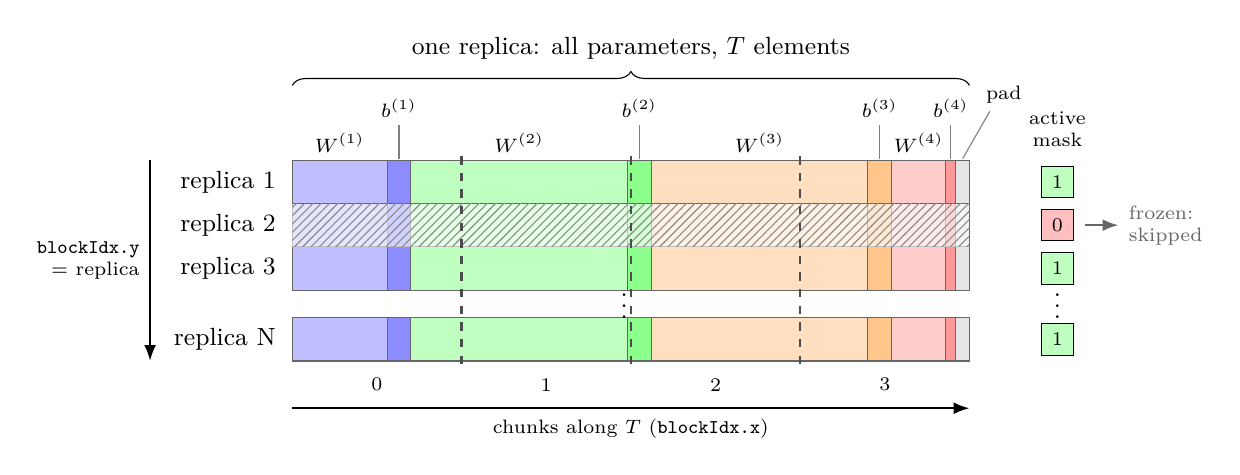
\begin{tikzpicture}[font=\small, x=0.86cm, y=1cm]
		% segments of one row: start / width / colour
		\def\rowh{0.55}
		\def\segs{0/1.4/blue!25, 1.4/0.35/blue!45, 1.75/3.2/green!25, 4.95/0.35/green!45, 5.3/3.2/orange!25, 8.5/0.35/orange!45, 8.85/0.8/red!20, 9.65/0.15/red!40, 9.8/0.2/black!10}
		\foreach \ytop/\lab/\mval/\mcol in {0/1/1/green!25, -0.55/2/0/red!25, -1.1/3/1/green!25, -2.0/N/1/green!25} {
			\foreach \x/\w/\c in \segs {
				\fill[\c] (\x,\ytop) rectangle ++(\w,-\rowh);
				\draw[black!60] (\x,\ytop) rectangle ++(\w,-\rowh);
			}
			\node[anchor=east] at (-0.1,\ytop-\rowh/2) {replica \lab};
			\node[draw, minimum size=4mm, inner sep=0pt, fill=\mcol, font=\scriptsize] at (11.3,\ytop-\rowh/2) {\mval};
		}
		% the frozen replica
		\fill[white, opacity=0.6] (0,-0.55) rectangle (10.0,-1.1);
		\fill[pattern=north east lines, pattern color=black!45] (0,-0.55) rectangle (10.0,-1.1);
		\node at (4.9,-1.75) {\(\vdots\)};
		\node at (11.3,-1.75) {\(\vdots\)};
		% column labels: weights in the lower row, biases and padding staggered above
		\foreach \x/\w/\lab in {0/1.4/W^{(1)}, 1.75/3.2/W^{(2)}, 5.3/3.2/W^{(3)}, 8.85/0.8/W^{(4)}} {
			\node[font=\scriptsize] at ({\x+\w/2},0.22) {\(\lab\)};
		}
		\foreach \x/\w/\lab in {1.4/0.35/b^{(1)}, 4.95/0.35/b^{(2)}, 8.5/0.35/b^{(3)}, 9.65/0.15/b^{(4)}} {
			\draw[black!50] ({\x+\w/2},0.02) -- ({\x+\w/2},0.45);
			\node[font=\scriptsize, anchor=south] at ({\x+\w/2},0.42) {\(\lab\)};
		}
		\draw[black!50] (9.9,0.02) -- (10.3,0.62);
		\node[font=\scriptsize, anchor=south west] at (10.1,0.6) {pad};
		\node[font=\scriptsize, align=center, anchor=south] at (11.3,0.05) {active\\mask};
		\draw[decorate, decoration={brace, amplitude=5pt}] (0,0.95) -- (10.0,0.95) node[midway, above=6pt] {one replica: all parameters, \(T\) elements};
		% frozen annotation
		\draw[-{Latex[length=2mm]}, thick, black!60] (11.7,-0.825) -- ++(0.5,0) node[right, align=left, font=\scriptsize] {frozen:\\skipped};
		% chunk grid
		\foreach \x in {2.5,5.0,7.5} \draw[dashed, thick, black!70] (\x,0.05) -- (\x,-2.65);
		\foreach \i/\x in {0/1.25,1/3.75,2/6.25,3/8.75} \node[font=\scriptsize] at (\x,-2.85) {\i};
		\draw[-{Latex[length=2mm]}, thick] (-2.1,0.0) -- (-2.1,-2.55) node[midway, left, font=\scriptsize, align=right] {\texttt{blockIdx.y}\\= replica};
		\draw[-{Latex[length=2mm]}, thick] (0,-3.15) -- (10.0,-3.15) node[midway, below, font=\scriptsize] {chunks along \(T\) (\texttt{blockIdx.x})};
	\end{tikzpicture}
	\caption[Consolidated parameter buffer of an ensemble and the launch grid of the fused optimizer]{The consolidated \((N, T)\) buffer holding the parameters of all \(N\) replicas of a four-layer MLP. Each row is one replica, with its weight matrices \(W^{(l)}\) and bias vectors \(b^{(l)}\) stored one after another and padded to a multiple of four elements. The gradients and the optimizer states share this layout. The fused optimizer covers the buffer with a two-dimensional grid of thread blocks, one grid row per replica and one column per chunk of the row (dashed lines). A replica frozen by early stopping (hatched, active mask 0) is skipped by all of its blocks.}
	\label{fig:tsConsolidated}
\end{figure}

With this layout the update of the whole ensemble is a single elementwise operation on a few \((N, T)\) matrices.
%
torchstrap implements it as fused kernels for the Adam optimizer~\cite{Kingma:2014adam}, including its variant with decoupled weight decay (AdamW~\cite{Loshchilov:2017adamw}) used in this thesis, and for SGD and Adagrad, with one C++ implementation for the CPU and one CUDA implementation for the GPU, registered as PyTorch operators.
%
A kernel reads each element of the parameters, gradients and moments once, updates it and writes it back, without allocating any temporary \((N, T)\) tensors, so it needs no more memory than a loop over replicas.
%
The GPU kernel is launched on the two-dimensional grid of Fig.~\ref{fig:tsConsolidated}, in which every block works on one chunk of one replica.
%
This makes the per-replica quantities cheap: the learning rate, the other hyperparameters and the step count used for the bias correction of Adam are read once per block from the \((N,)\) vectors, and a block whose replica is frozen returns immediately, so a frozen replica costs no memory traffic and its parameters remain exactly unchanged.
%
The arithmetic of the update is taken from the fused optimizers of PyTorch itself, and for every active replica the result is bit-for-bit identical to that of \texttt{torch.optim.Adam} with \texttt{fused=True}, which is enforced by the tests of the library.
%
The optimizer also composes with \texttt{vmap}, so the complete training step, forward pass, backward pass and parameter update, is written for one model and vectorized as a whole.

Tab.~\ref{tab:tsBenchmark} compares one Adam step of torchstrap with the straightforward alternative of \(N\) independent PyTorch optimizers stepped in a loop, for an MLP of the size used for the toy example below.
%
The speed-up is largest for small ensembles, where the launch overhead dominates, and settles at about a factor of three once the ensemble is large enough for the update to be limited by the memory bandwidth.
%
Late in a training, when early stopping has frozen most replicas, the skipped rows make the update another factor of four faster.

\begin{table}[htbp]
	\caption[Timing of one optimizer step for an ensemble]{Time of one Adam step for an ensemble of \(N\) MLP replicas with six parameter tensors and 265k parameters each, in single precision on an NVIDIA RTX 4070 Laptop GPU (median of 20 runs). The loop steps \(N\) independent \texttt{torch.optim.Adam} optimizers; torchstrap updates the consolidated buffer with one fused kernel. The peak memory is the same for both. The last row has 75\% of the replicas frozen.}
	\label{tab:tsBenchmark}
	\centering
	\begin{tabular}{r | r r | c}
		\hline
		\(N\) & Loop & torchstrap & Speed-up \Tstrut \Bstrut \\
		\hline
		8 & 796~\(\mu\)s & 140~\(\mu\)s & 5.7 \\
		32 & 3.22~ms & 1.18~ms & 2.7 \\
		100 & 9.38~ms & 3.23~ms & 2.9 \\
		100, 75\% frozen & -- & 0.80~ms & 4.0 (vs.\ all active) \\
		\hline
	\end{tabular}
\end{table}

\section{Toy example}
\label{sec:tsToy}
The effect of the three configurations of Fig.~\ref{fig:tsEnsembles} is illustrated with the two-spirals example of the torchstrap repository: a classifier separating two interleaved spirals of 100 points in total, smeared with Gaussian noise, a problem in which the decision boundary is only constrained where there are data.
%
An MLP with two hidden layers of 512 nodes is trained with Adam and a cosine learning-rate schedule, once as a single model and twice as an ensemble of 100 replicas trained in parallel, and the predicted probability of the classifier is shown in Fig.~\ref{fig:tsSpirals}.
%
The single model (left) draws a sharp boundary that separates the training points and extends arbitrarily into the regions without data.
%
An ensemble trained on the same data (middle) differs only through the initialization of its replicas, and its mean prediction is nearly identical to the single model, since all replicas learn the same points.
%
When every replica is trained on its own bootstrap resample (right), the replicas disagree where the data do not constrain the boundary, and the mean prediction is softened there, most visibly away from the spiral arms, while it stays confident where the points are dense.
%
This spread of the replicas is the quantity that Sec.~\ref{sec:bootstrap} uses as the statistical uncertainty of the unfolded distributions.

\begin{figure}[htbp]
	\centering
	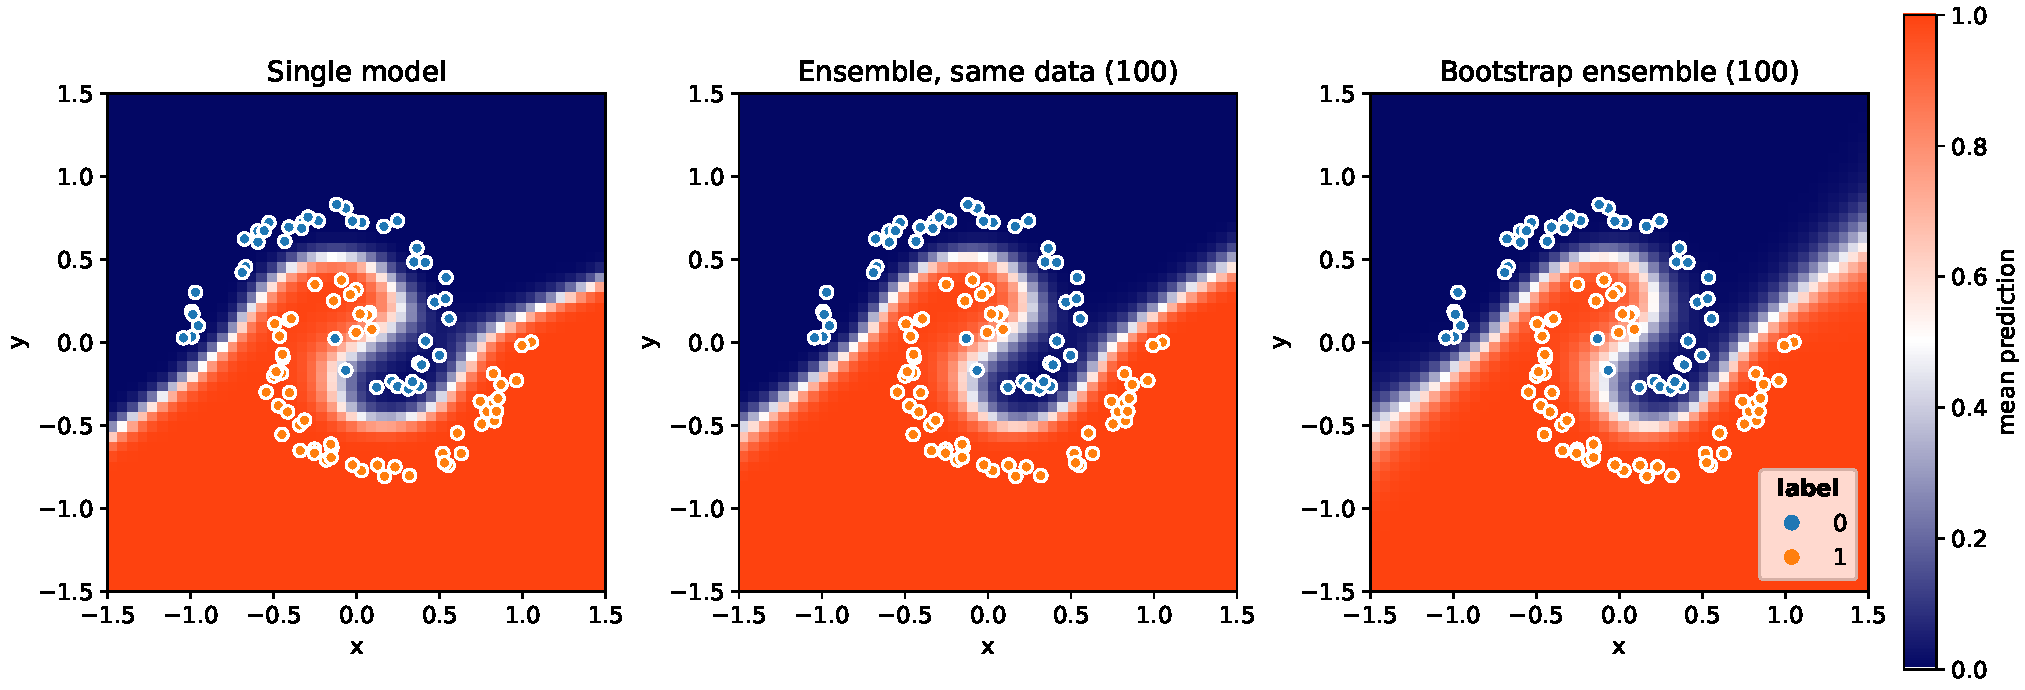
\includegraphics[width=\linewidth]{figures/torchstrap/spirals_predictions.pdf}
	\caption[Predictions of a single MLP and of MLP ensembles on the two-spirals problem]{Predicted probability of an MLP classifier trained on 100 points from two noisy spirals (blue: class 0, orange: class 1), for a single model (left), the mean of an ensemble of 100 replicas trained on the full dataset (middle), and the mean of a bootstrap ensemble of 100 replicas, each trained on its own resample (right). All replicas of an ensemble were trained simultaneously on one GPU.}
	\label{fig:tsSpirals}
\end{figure}

A bootstrap resample leaves out about 37\% of the points, which gives every replica a held-out \emph{out-of-bag} sample without a separate validation split.
%
The bootstrap ensemble uses it to monitor its training: the out-of-bag loss of every replica is computed in the same vectorized pass as the predictions and drives the per-replica learning-rate schedule, checkpointing and early stopping.
%
Fig.~\ref{fig:tsTraining} shows the resulting training history.
%
The training and out-of-bag losses of the replicas fall together for the first five epochs, after which the training loss keeps decreasing while the out-of-bag loss levels off at about 0.1, the onset of overfitting that the checkpoints of the best epoch guard against.
%
The out-of-bag loss of the individual replicas (right) differs by up to a factor of a few, reflecting the different points each replica was trained on, and the loss of the ensemble-averaged prediction lies below the mean loss of the replicas.

\begin{figure}[htbp]
	\centering
	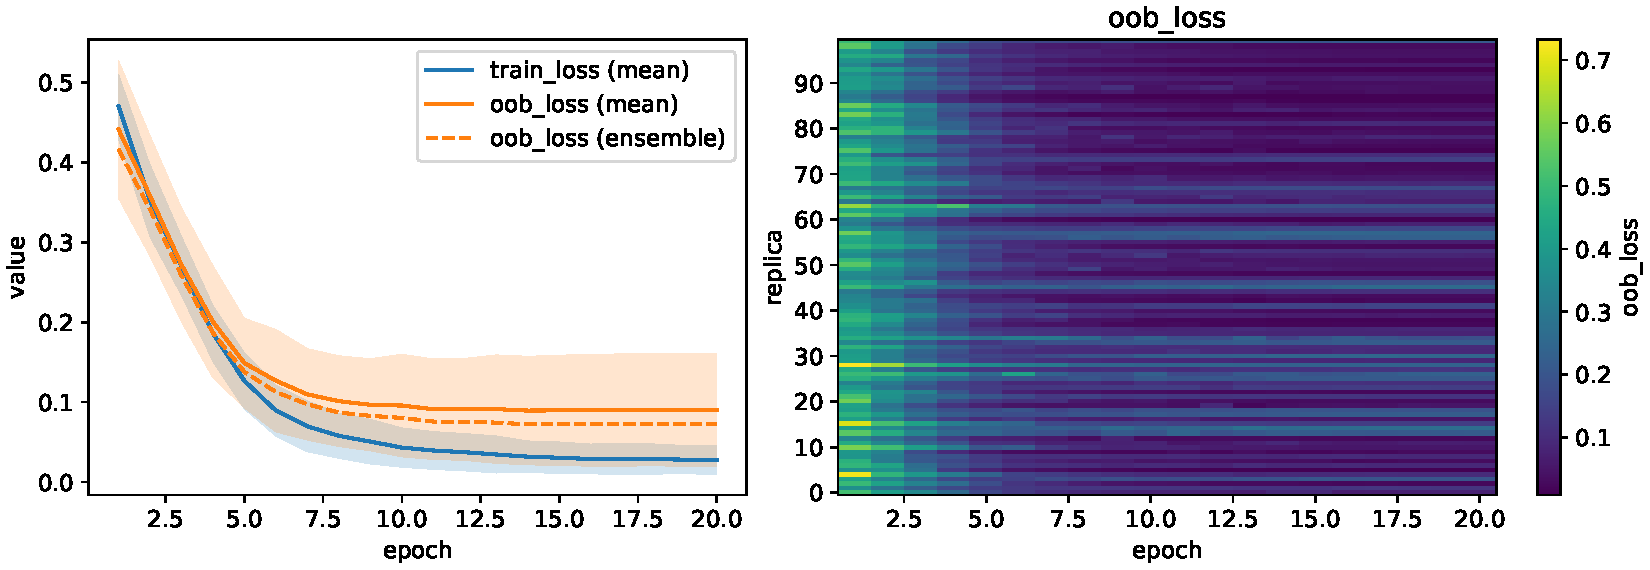
\includegraphics[width=\linewidth]{figures/torchstrap/spirals_training.pdf}
	\caption[Training history of the bootstrap ensemble of the two-spirals example]{Training history of the bootstrap ensemble of Fig.~\ref{fig:tsSpirals}. (Left) Training loss (blue) and out-of-bag loss (orange) averaged over the 100 replicas, with bands showing their spread, and the out-of-bag loss of the ensemble-averaged prediction (dashed). (Right) Out-of-bag loss of every replica (rows) in every epoch (columns).}
	\label{fig:tsTraining}
\end{figure}

\section{Use in this thesis}
\label{sec:tsUse}
In the MultiFold unfolding of the \pp measurement (Sec.~\ref{sec:ppUnfolding}), each of the four classifiers of an iteration is a torchstrap ensemble, and the replica index is carried through all classifiers and iterations, so that replica \(k\) is a complete unfolding of its own (Eq.~\ref{eq:replicaWeight}).
%
The per-replica subsamples of measured and simulated jets, the per-replica early stopping on the validation loss and the per-replica training histories of Fig.~\ref{fig:unfoldigLossAccAUC} are all provided by the mechanisms described above.
%
Because a frozen replica neither changes nor costs anything, the ensemble can be trained until its slowest replica has converged without degrading those that stopped earlier.
%
The whole ensemble, and with it the full set of systematic variations of Sec.~\ref{sec:ppSystematics}, were trained on a single laptop GPU, an NVIDIA RTX 4070 Laptop GPU with 8~GB of memory.



\clearpage

\pagestyle{empty}
%\input{vita}

\end{document}
